\documentclass[11pt, a4paper]{article}

\usepackage{style}

\institution{EPFL}
\project{Semester Project}
\degree{Master of Science MSc in \\ Computational Science and Engineering}
\title{Minimal Rational Interpolation for Time-Harmonic Maxwell's Equations}
\author{Fabio Matti}
\supervisor{Prof. Fabio Nobile \\ Dr. Davide Pradovera}
\date{\today}

\begin{document}

\maketitle

\begin{abstract}
    \acrfull{MRI} provides an efficient and reliable way to approximate
    a meromorphic dependence of a characteristic output quantity of a model on one
    of its parameters.
    The focus of this report is on the \acrfull{gMRI} algorithm and particularly
    on ways to enhance its performance. This algorithm is then applied to three 
    example problems concerning the time-harmonic Maxwell's equations in the 
    frequency domain. The advantages and disadvantages of
    \acrshort{gMRI} as compared to conventional approaches for finding quantities
    such as resonant modes that are of interest for problems of this type are discussed.
    Furthermore, the application of the \acrshort{gMRI} algorithm for finding the 
    scattering coefficients of a \acrfull{DMCWF} is studied.
\end{abstract}

\newpage
\tableofcontents

\newpage
\section{Introduction}
\label{sec:introduction}

%!REMINDME (rewrite introduction)

%A wide class of problems in physics and engineering concern studying
%the dependence of a model on one (or more) of its parameters $\omega$. 
%Of interest is usually a characteristic quantity
%$\mathbf{u}(\omega)$ depending on this parameter.
%Unless the system allows for an analytical solution, one may usually only
%find numerical solutions to the system for discrete values of the parameter.
\acrfull{MRI} offers a way to locally approximate vector fields
$\mathbf{u}:\mathbb{C}\ni\omega\mapsto \mathbf{u}(\omega)$
which exhibit a meromorphic dependence on one of their 
parameters $\omega$. This approximation allows us to study the response of the
system with respect to $\omega$ such as identifying values for the parameter
$\omega$ for which resonance occurs. The approach has proven
effective and efficient (both memory- and time-wise) in applications
on Helmholtz-type problems \cite{greedyMRI, shortMRI}. Due to the presence of 
resonances at which the $\mathbf{u}$ theoretically becomes singular, classical
approaches such as Lagrangian approximation usually fail.

Central to this report are time-harmonic electromagnetic problems, whose 
parameter is the (angular) frequency. These problems are governed by
the time-harmonic Maxwell's equations. Choosing the quantity of interest
to be a vector potential, these equations reduce to the curl-curl equation
\begin{equation}
    \nabla \times (\mu^{-1} \nabla \times \mathbf{u}) - \epsilon \omega^2 \mathbf{u} = \mathbf{j}
\end{equation}
A justification for why a rational interpolation approach is appropriate for
this class of problems will be presented in Section \ref{subsec:motivation}.

The first few pages in this report are a short guide for finding numerical 
solutions to the time-harmonic Maxwell's equations using the \acrfull{FEM}.
These solutions are then used in the core of this report, which gives a description
of the \acrfull{gMRI} algorithm. Properties of and optimization tricks for the
\acrshort{gMRI} are shown. In the end, three applications of the method are studied and
discussed: the resonant modes of a two-dimensional resonant cavity,
the two-dimensional cavity with an imperfectly conducting boundary, and lastly
the scattering coefficients of a \acrfull{DMCWF}.

My implementations can be found in \cite{git}. Vectors are printed in \textbf{bold}
while matrices additionally have an \textbf{\underline{underline}}. 
Euclidean scalar products are denoted with $\langle \cdot , \cdot \rangle$
and norms with $||\cdot||$. The identity matrix shall be printed as $\mathbf{\underline{Id}}$.
The Hermitian transpose is written as $^{H}$. For simplicity, results are delivered without units
and the angular frequency is referred to simply by frequency.

\newpage
\section{Finite element discretization of the time-harmonic Maxwell's equations}
\label{sec:maxwell}

\acrfull{MRI} requires the knowledge of the solution of the problem for discrete 
values of the model parameter that is of interest. A way of obtaining these
solutions is the \acrfull{FEM}. For that purpose, I now derive a strong formulation
for the time-harmonic Maxwell problem and subsequently convert it to its
corresponding weak formulation.

\subsection{Vector potential formulation of the time-harmonic Maxwell's equations}
\label{subsec:maxwell-potential}

% Everything smooth enough to do all manipulations...
I assume that all quantities in this section are smooth enough to perform the
necessary vector calculus manipulations.

Let $\mathbf{E}$ denote an electric field, $\mathbf{B}$ a magnetic field
strength, $\rho$ an electric charge density, and $\mathbf{j}$ an electric
current density. Maxwell's equations are stated in \citep{monk} as
\begin{align}
    \langle \nabla, \epsilon \mathbf{E} \rangle &= \rho \label{equ:maxwell1} \\
    \langle \nabla, \mathbf{B} \rangle &= 0 \label{equ:maxwell2} \\
    \nabla \times \mathbf{E} &= -\partial_t \mathbf{B} \label{equ:maxwell3} \\
    \nabla \times (\mu^{-1} \mathbf{B}) &= \partial_t (\epsilon \mathbf{E}) + \mathbf{j} \label{equ:maxwell4}
\end{align}
with $\varepsilon$ being the permittivity and $\mu$ the permeability.

Equation (\ref{equ:maxwell2}) motivates the expression of the magnetic field 
$\mathbf{B} = \nabla \times \mathbf{u}$ in terms of a vector-valued function
$\mathbf{u}$, the vector potential (in literature commonly denoted with
$\mathbf{A}$). Similarly, (\ref{equ:maxwell3}) suggests
rewriting the electric field $\mathbf{E} = - \nabla \phi - \partial_t \mathbf{u}$
using a scalar function $\phi$, referred to as the scalar potential.

The physical quantities $\mathbf{E}$ and $\mathbf{B}$ remain unchanged 
if we transform $\mathbf{u} \to \mathbf{u}' = \mathbf{u} + \nabla \psi$ or
$\phi \to \phi' = \phi - \partial_t \psi$ for an arbitrary function $\psi$.
A convenient choice of $\psi$ is suggested in \citep{gauge-transformation} to be
\begin{equation}
    \psi = \int_0^t \phi dt' \label{equ:gauge}
\end{equation}
which transforms $\phi \to \phi' = 0$ and $\mathbf{u} \to \mathbf{u}' = \mathbf{u}
+ \nabla \int_0^t \phi dt'$. Thus, the expressions for the electrical and
magnetic field become
\begin{align}
    \mathbf{E} &= -\partial_t \mathbf{u} \label{equ:electricfield} \\
    \mathbf{B} &= \nabla \times \mathbf{u} \label{equ:magneticfield}
\end{align}
where I have subtly renamed the variable $\mathbf{u}'$ to $\mathbf{u}$ for simplicity.

Plugging the identities (\ref{equ:electricfield}) and (\ref{equ:magneticfield})
into (\ref{equ:maxwell4}) yields (assuming a static permittivity $\epsilon$)
\begin{equation}
    \nabla \times (\mu^{-1} \nabla \times \mathbf{u}) = - \epsilon \partial_t^2 \mathbf{u} + \mathbf{j} \label{equ:maxwell-potential}
\end{equation}

For the rest of this report, I restrict myself to vector potentials $\mathbf{u}$
that exhibit a harmonic dependence on time $t$, i.e. may be factorized into
a term solely depending on the position $\mathbf{x}$ and a complex exponential
depending on time
\begin{equation}
    \mathbf{u}(\mathbf{x}, t) = \mathbf{u}(\mathbf{x}) \exp(i \omega t) \label{equ:time-harmonic}
\end{equation}
Substituting this expression into (\ref{equ:maxwell-potential}) and rearranging 
a little results in the
\begin{fancybox}{Time-harmonic potential equation}
    \begin{equation}
     \nabla \times (\mu^{-1} \nabla \times \mathbf{u}) - \epsilon \omega^2 \mathbf{u} = \mathbf{j} \label{equ:maxwell-timeharmonic}
    \end{equation}
\end{fancybox}

\subsection{Weak formulation for the time-harmonic potential equation}
\label{subsec:maxwell-weak}

Take the inner product of equation (\ref{equ:maxwell-timeharmonic}) with an arbitrary
vector-valued test function $\mathbf{v} \in H_{\textrm{curl}}(\Omega)$, where
\begin{equation}
    H_{\textrm{curl}}(\Omega) = \{\mathbf{v} : \Omega \to \mathbb{C}^3,~\text{such that}~\mathbf{v}\in L_2(\mathbb{C})^3, \nabla \times \mathbf{v} \in L_2(\mathbb{C})^3\} \label{equ:h-curl}
\end{equation}
and then integrate over the whole computational domain $\Omega$ to obtain 
\begin{equation}
    \int_{\Omega} \langle \nabla \times ({\mu^{-1} \nabla \times \mathbf{u}}), \mathbf{v} \rangle
    - \omega^2 \int_{\Omega} \epsilon \langle \mathbf{u}, \mathbf{v} \rangle =
    \int_{\Omega} \langle \mathbf{j}, \mathbf{v} \rangle \label{equ:maxwell-weak-initial}
\end{equation}
Equation (\ref{equ:maxwell-weak-initial}) may be further simplified to:
\begin{fancybox}{Weak formulation of the time-harmonic potential equation}
    \begin{equation}
        \int_{\Omega} \langle {\mu^{-1} \nabla \times \mathbf{u}}, \nabla \times \mathbf{v} \rangle
        - \omega^2 \int_{\Omega} \epsilon \langle \mathbf{u}, \mathbf{v} \rangle
        = \int_{\Omega} \langle \mathbf{j}, \mathbf{v} \rangle
        + \int_{\partial \Omega} \langle \underbrace{({\mu^{-1} \nabla \times \mathbf{u}}) \times \mathbf{n}}_{= \mathbf{g}}, \mathbf{v} \rangle
        \label{equ:maxwell-weak}
    \end{equation}
\end{fancybox}
where $\mathbf{n}$ denotes the outward surface normal to the boundary $\partial \Omega$
of the computational domain $\Omega$ and $\mathbf{v}$ is an arbitrary element
of $H_{\textrm{curl}}(\Omega)$. I allow myself
to spare you the details of this computation, but nevertheless put a proper derivation
in the appendix at the end of this report.

Supposing that we know the electric field $\mathbf{E}$ along a part of the
boundary $\Gamma \subset \partial \Omega$, we may most easily enforce it
in a Dirichlet-type fashion through the relation (\ref{equ:electricfield}) and
the assumption (\ref{equ:time-harmonic})
\begin{equation}
    \left.\mathbf{u}\right|_{\Gamma} = -\frac{1}{i\omega} \left.\mathbf{E}\right|_{\Gamma} \label{equ:dirichlet-boundary}
\end{equation}
A known magnetic field $\mathbf{B}$ may similarly be enforced
with a Neumann-type condition following
from (\ref{equ:magneticfield}) and (\ref{equ:time-harmonic})
\begin{equation}
    \left.\mathbf{g}\right|_{\Gamma} = (\mu^{-1} \left.\mathbf{B}\right|_{\Gamma}) \times \mathbf{n} \label{equ:neumann-boundary}
\end{equation}

\subsection{Examples}
\label{subsec:examples}

I will now specialize and simplify this weak formulation for three different
applications which will be studied in Section \ref{sec:examples}. To see
that these problems are intimately related, I refer you to Figure \ref{fig:examples}.

\begin{figure}[h]
    \centering
    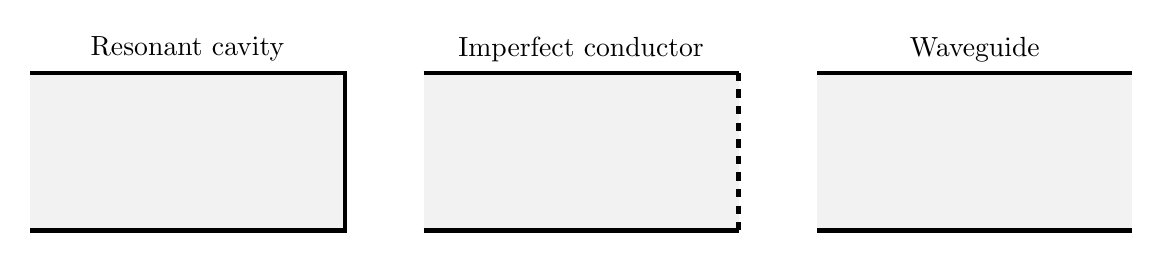
\begin{tikzpicture}
    \node at (2, 2.3) {Resonant cavity};
    \fill[black!5!white] (0, 0) rectangle (4, 2);
    \draw[ultra thick] (0, 0) to (4, 0) to (4, 2) to (0, 2);

    \node at (7, 2.3) {Imperfect conductor};
    \fill[black!5!white] (5, 0) rectangle (9, 2);
    \draw[ultra thick] (5, 0) to (9, 0);
    \draw[ultra thick, dashed] (9, 2) to (9, 0);
    \draw[ultra thick] (5, 2) to (9, 2);

    \node at (12, 2.3) {Waveguide};
    \fill[black!5!white] (10, 0) rectangle (14, 2);
    \draw[ultra thick] (10, 0) to (14, 0);
    \draw[ultra thick] (10, 2) to (14, 2);
\end{tikzpicture}
    \caption{Schematic visualization of the most trivial case for each of the
    boundary configurations that will be analyzed in Section \ref{sec:examples}.
    The perfectly conducting boundaries are drawn in black, while the imperfectly
    conducting boundary appears dashed. Inlets and outlets are left unmarked.}
    \label{fig:examples}
\end{figure}

\subsubsection{Two-dimensional resonant cavity}
\label{subsubsec:cavity}

I refer to a resonant cavity as a region $\Omega$ enclosed by a boundary $\partial \Omega$.
The boundary can be subdivided into one (or more) inlets $\Gamma_N$ and a perfectly
conducting wall $\Gamma_D = \partial \Omega \setminus \Gamma_N$
(see Figure \ref{fig:2d-cavity} for an abstract visualization of such a cavity).

\begin{figure}[h]
    \centering
    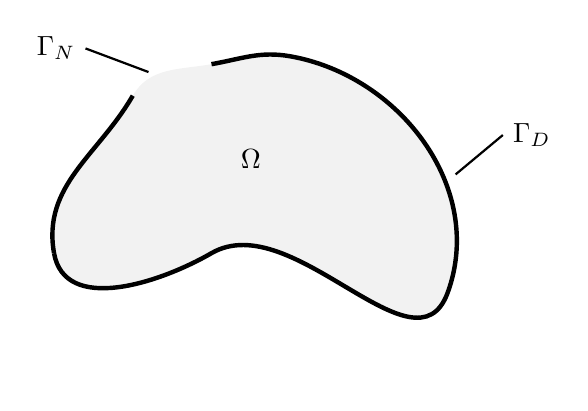
\begin{tikzpicture}
    \fill[black!5!white] (2, 1) to [out=100, in=240] (3, 3)
                              to [out=60, in=190] (4, 3.4)
                              to [out=10, in=170] (5, 3.5)
                              to [out=350, in=70] (7, 0.5)
                              to [out=250, in=30] (4, 1)
                              to [out=210, in=280] (2, 1);
    \draw[ultra thick] (2, 1) to [out=100, in=240] (3, 3);

    \draw[ultra thick] (4, 3.4) to [out=10, in=170] (5, 3.5)
                              to [out=350, in=70] (7, 0.5)
                              to [out=250, in=30] (4, 1)
                              to [out=210, in=280] (2, 1);
    \draw[thick] (2.4, 3.6) node[left] {$\Gamma_N$} to (3.2, 3.3);
    \draw[thick] (7.7, 2.5) node[right] {$\Gamma_D$} to (7.1, 2);
    \node at (4.5, 2.2) {$\Omega$};
\end{tikzpicture}
    \caption{An abstract example of a two-dimensional resonant cavity enclosing
    a domain $\Omega$ with a perfectly conducting boundary $\Gamma_D$ and
    featuring a single inlet $\Gamma_N$.}
    \label{fig:2d-cavity}
\end{figure}

Now, we move down to two dimensions, i.e. assume the resonant cavity lies in a plane.
Suppose the current density $\mathbf{j} \equiv 0$ and orient the coordinate
system in such a way that $\mathbf{u} = u_z \mathbf{e}_z$ and 
$\mathbf{v} = v_z \mathbf{e}_z$. Consequently, the scalar product of the two 
curls in Equation (\ref{equ:maxwell-weak}) simplifies to the scalar product 
of two gradients:
\begin{equation}
    \langle \mu^{-1} \nabla \times \mathbf{u}, \nabla \times \mathbf{v} \rangle
    = \langle \mu^{-1} \nabla u_z, \nabla v_z \rangle
\end{equation}
Denote by $g_z$ the component of $\mathbf{g}$ in the $z$-direction along the
inlet $\Gamma_N$. These simplifications allow the conversion of 
(\ref{equ:maxwell-weak}) into the weak formulation for a two-dimensional
resonant cavity
\begin{equation}
    \int_{\Omega} \langle \mu^{-1} \nabla u_z, \nabla v_z \rangle
    - \omega^2 \int_{\Omega} \epsilon u_z v_z^{\ast}
    = \int_{\partial \Omega} g_z v_z^{\ast} \label{equ:maxwell-weak-resonant-cavity}
\end{equation}
for an arbitrary $v_z \in H_1(\Omega) = \{v : \Omega \to \mathbb{C},~\text{such that}~\mathbf{v}\in L_2(\mathbb{C}), \nabla v \in L_2(\mathbb{C})^2\}$.
% Boundary conditions Dirichlet and Neumann (from Monk)
Now, let $\mathbf{E}$ and $\mathbf{B}$ refer to the electric and magnetic fields inside
the cavity. For now, I distinguish between two types of boundaries:

For the perfectly conducting boundary $\Gamma_D$, treated in \citep{monk}, it holds that
\begin{equation}
    \mathbf{n} \times \mathbf{E} = \mathbf{0},~~\text{on}~\Gamma_D \label{equ:perfect-conductor-boundary}
\end{equation}
For the boundaries in a two-dimensional resonant cavity (see Figure 
\ref{fig:2d-cavity}), this only holds true if $E_z = 0$, which translates
to the Dirichlet boundary condition $\left.u_z\right|_{\Gamma_D} = 0$
in light of (\ref{equ:dirichlet-boundary}).

For the inlet, it is easiest to enforce the boundary condition through the
magnetic field $\mathbf{B}$ in exactly the way proposed in
(\ref{equ:neumann-boundary}) (assuming $\mathbf{n} = -\mathbf{e}_x$ as
will always be the case in Section \ref{sec:examples}, cf. Figure \ref{fig:rectangular_cavity}):
\begin{equation}
    g_z = (({\mu^{-1} \mathbf{B}}) \times (-\mathbf{e}_x))_z = \mu^{-1} B_x,~~\text{on}~\Gamma_N
\end{equation}

\subsubsection{Imperfect conductor}
\label{subsubsec:impedance}

% Additionally impedance boundary condition from Monk
To simulate an imperfect boundary $\Gamma_I$, also called impedance boundary in literature, 
\cite{monk} suggests replacing the integrand $\mathbf{g}$ that appeared in 
(\ref{equ:maxwell-weak}) with
\begin{equation}
    \mathbf{g} = (\mu^{-1} \nabla \times \mathbf{u}) \times \mathbf{n}
    = i \omega \lambda (\mathbf{n} \times \mathbf{u}) \times \mathbf{n}~~\text{on}~\Gamma_I
    \label{equ:impedance-boundary-g}
\end{equation}
with a parameter $\lambda>0$ which I will henceforth refer to as the impedance.
Supposing that $\mathbf{u} = u_z \mathbf{e}_z$ and only treating a
two-dimensional domain, this condition simplifies to
\begin{equation}
    g_z = i \omega \lambda u_z~~\text{on}~\Gamma_I
\end{equation}
by using the fact that $\mathbf{n} \perp \mathbf{u}$
and $||\mathbf{n}|| = 1$, so $(\mathbf{n} \times \mathbf{u}) \times \mathbf{n} = \mathbf{u}$,
as is demonstrated in the appendix at the end of this report.

\subsubsection{Waveguide}
\label{subsubsec:waveguide}

% Just j=0 and 3d, need to discuss boundary conditions
Going back to (\ref{equ:maxwell-weak}) and this time staying in three dimensions,
we again assume no electric current density $\mathbf{j} \equiv 0$ is present.
I suppose that the inlet is located at a constant $x$-value,
such that the surface normal to this inlet is $-\mathbf{e}_x$. Conveniently, the example 
in Section \ref{subsec:examples-dmcwf} happens to be set up in just this way. For an incoming
magnetic field at the inlet $\Gamma_i$ with $\left.\mathbf{B}\right|_{\Gamma_i} = B_0 \mathbf{e}_y$,
we see from (\ref{equ:neumann-boundary}) that this may be modelled by setting
$\left.\mathbf{g}\right|_{\Gamma_i} = - \mu^{-1} B_0 \mathbf{e}_z$.
At the \enquote{outlet} $\Gamma_o$, we set $\left.\mathbf{g}\right|_{\Gamma_o} = \boldsymbol{0}$.

\newpage
\section{Finite element approximation with FEniCS}
\label{sec:fem}

Based on the weak formulation corresponding to the time-harmonic potential equation
(\ref{equ:maxwell-weak}), the \acrfull{FEM} can be used to approximate solutions 
to Equation (\ref{equ:maxwell-timeharmonic}).

\subsection{The Galerkin method}
\label{subsec:fem-theory}

% Theory
It is readily seen that the weak formulation (\ref{equ:maxwell-weak}) assumes the form
\begin{equation}
    \text{Find}~\mathbf{u} \in H_{\textrm{curl}}(\Omega),~\text{such that}~a_{\omega}(\mathbf{u}, \mathbf{v}) = L(\mathbf{v}), ~\forall \mathbf{v} \in H_{\textrm{curl}}(\Omega)
\end{equation}
with the bilinear form
\begin{equation}
    a_{\omega}(\mathbf{u}, \mathbf{v}) = \underbrace{\int_{\Omega} \langle \mu^{-1} \nabla \times \mathbf{u}, \nabla \times \mathbf{v}\rangle }_{K(\mathbf{u}, \mathbf{v})}
    - \omega^2 \underbrace{\int_{\Omega} \epsilon \langle \mathbf{u}, \mathbf{v} \rangle}_{M(\mathbf{u}, \mathbf{v})} \label{equ:bilinear-form}
\end{equation}
composed with the stiffness form $K(\mathbf{u}, \mathbf{v})$ and the mass form $M(\mathbf{u}, \mathbf{v})$, and
the linear form 
\begin{equation}
    L(\mathbf{u}) = \int_{\Omega} \langle \mathbf{j}, \mathbf{v} \rangle + \int_{\partial \Omega} \langle \mathbf{g}, \mathbf{v} \rangle \label{equ:linear-form}
\end{equation}
and the appropriate Hilbert space $H_{\textrm{curl}}(\Omega)$ defined in (\ref{equ:h-curl}).
Notice that in the case of the imperfectly conducting boundary, the integral along
the boundary will have to be moved from the linear to the bilinear form, since then 
$\mathbf{g}$ will depend on $\mathbf{u}$ via (\ref{equ:impedance-boundary-g}).

A sequence of appropriate finite dimensional spaces $H_{\textrm{curl}, h}(\Omega)$
parametrized by $h$ is introduced. As $h \to 0$, this sequence should become dense
in $H_{\textrm{curl}}(\Omega)$, loosely meaning that for any element in $H_{\textrm{curl}}(\Omega)$
we may find a sequence $w_h \in H_{\textrm{curl}, h}(\Omega)$ which approximates this
element arbitrarily well in the limit. The Galerkin problem is then formulated as
(see \cite{numapproxPDEs} for details)
\begin{fancybox}{Galerkin problem for the time-harmonic potential equation}
    \begin{equation}
        \text{Find}~\mathbf{u}_h \in H_{\textrm{curl},h}(\Omega),~\text{such that}~a_{\omega}(\mathbf{u}_h, \mathbf{v}_h) = L(\mathbf{v}_h), ~\forall \mathbf{v}_h \in H_{\textrm{curl}, h}(\Omega) \label{equ:galerkin-problem}
    \end{equation}
\end{fancybox}
One class of finite elements, the Nédélec elements of the first
kind, are particularly well suited for discretizing curl-curl-problems of the type
we have derived in Section \ref{sec:maxwell} (see \cite{monk}).

I refer to the \acrshort{FEM} matrix representations in the vertex basis of the forms
$K(\mathbf{u}, \mathbf{v})$ and $M(\mathbf{u}, \mathbf{v})$ distinguished in
(\ref{equ:bilinear-form}) as the
stiffness matrix $\mathbf{\underline{K}}$ and mass matrix $\mathbf{\underline{M}}$.

\subsection{Numerical approximation of \acrshort{PDE}s using FEniCS}
\label{subsec:fem-demo}

% Demonstration
FEniCS\footnote{\url{https://fenicsproject.org/}} bundles a collection of Python
modules designed to automate solving a \acrfull{PDE}.
Inspired by the demonstrations encountered in \cite{fenics}, I will now guide you
through a simple example, relevant to the context of this report to
show the process of obtaining approximate solutions to \acrshort{PDE}s with FEniCS.

Consider the time-harmonic potential equation (\ref{equ:maxwell-timeharmonic})
with the computational domain $\Omega$ being a cubic cavity with an inlet $\Gamma_N$
on one of its sides, but all other boundaries being perfect conductors.
Set $\mu = \epsilon = 1$ and $\mathbf{j} = 0$ for simplicity.

The \texttt{fenics} package is imported along with \texttt{numpy} for array manipulations.
\lstinputlisting[firstnumber=1, firstline=2, lastline=3]{code/fenics_example.py}

A mesh for the cubic cavity $\Omega$ is generated by dividing the cube into a
$10\times10\times10$ grid, whose cells are again subdivided into tetrahedrons.
\lstinputlisting[firstnumber=5, firstline=6, lastline=7]{code/fenics_example.py}

Our function space $H_{\textrm{curl},h}(\Omega)$ is composed using piecewise
linear Nédélec elements of the first kind.
\lstinputlisting[firstnumber=9, firstline=10, lastline=10]{code/fenics_example.py}

The inlet is introduced at $x = 0$.
\lstinputlisting[firstnumber=12, firstline=13, lastline=15]{code/fenics_example.py}

All other boundaries are perfectly conducting walls.
\lstinputlisting[firstnumber=17, firstline=18, lastline=20]{code/fenics_example.py}

A mesh function is used to identify the different boundaries. It evaluates to
0, if a vertex is not on any boundary; 1 if the vertex is a the inlet; and 2 if
the vertex sits on a perfectly conducting boundary.
\lstinputlisting[firstnumber=22, firstline=23, lastline=26]{code/fenics_example.py}

For Nédélec elements of the first kind, (\ref{equ:perfect-conductor-boundary})
is enforced through
\lstinputlisting[firstnumber=28, firstline=29, lastline=30]{code/fenics_example.py}

Let $\mathbf{g} = \mathbf{e}_z$ in (\ref{equ:neumann-boundary}), which corresponds
to a magnetic field $\mu^{-1} \mathbf{B} = \mathbf{e}_y$, and define a boundary
measure.
\lstinputlisting[firstnumber=32, firstline=33, lastline=34]{code/fenics_example.py}

Trial and test functions for the function space $H_{\mathrm{curl},h}(\Omega)$ are
instantiated to express the weak formulation (cf. Equation \ref{equ:maxwell-weak}).
\lstinputlisting[firstnumber=36, firstline=37, lastline=38]{code/fenics_example.py}

The linear form (\ref{equ:linear-form}) is assembled.
\lstinputlisting[firstnumber=40, firstline=41, lastline=41]{code/fenics_example.py}

The stiffness matrix (i.e. the first term in the bilinear form (\ref{equ:bilinear-form}))
is assembled, and the Dirichlet boundary conditions are applied.
\lstinputlisting[firstnumber=43, firstline=44, lastline=45]{code/fenics_example.py}

The mass matrix (i.e. the second term in the bilinear form (\ref{equ:bilinear-form}))
is assembled. The fact that the Dirichlet boundary conditions have already
been separately applied to the stiffness matrix above is accounted for by setting
all rows and columns corresponding to degrees of freedom on the Dirichlet
boundary to zero.
\lstinputlisting[firstnumber=47, firstline=48, lastline=49]{code/fenics_example.py}

A function to compute an approximation of the $L_2(\Omega)$-norm of a solution
to the system can be created. Notice how I can reuse the mass matrix
$\mathbf{\underline{M}}$ for this purpose only due to the fact that
$\epsilon = 1$ was taken.
\lstinputlisting[firstnumber=51, firstline=52, lastline=54]{code/fenics_example.py}

Finally, for 200 uniformly spaced frequencies $\omega \in [6.2, 6.8]$, the 
approximate solution to the cubic cavity at each of these frequencies is
computed and its $L_2(\Omega)$-norm memorized for later.
\lstinputlisting[firstnumber=56, firstline=57, lastline=62]{code/fenics_example.py}

What results is an approximation of the frequency response in the $L_2(\Omega)$-norm
for the cubic cavity (see Figure \ref{fig:fenics-demonstration}). 
\begin{figure}[h]
    \centering
    %% Creator: Matplotlib, PGF backend
%%
%% To include the figure in your LaTeX document, write
%%   \input{<filename>.pgf}
%%
%% Make sure the required packages are loaded in your preamble
%%   \usepackage{pgf}
%%
%% Also ensure that all the required font packages are loaded; for instance,
%% the lmodern package is sometimes necessary when using math font.
%%   \usepackage{lmodern}
%%
%% Figures using additional raster images can only be included by \input if
%% they are in the same directory as the main LaTeX file. For loading figures
%% from other directories you can use the `import` package
%%   \usepackage{import}
%%
%% and then include the figures with
%%   \import{<path to file>}{<filename>.pgf}
%%
%% Matplotlib used the following preamble
%%   \usepackage{fontspec}
%%   \setmainfont{DejaVuSans.ttf}[Path=\detokenize{C:/Users/Fabio/Anaconda3/Lib/site-packages/matplotlib/mpl-data/fonts/ttf/}]
%%   \setsansfont{DejaVuSans.ttf}[Path=\detokenize{C:/Users/Fabio/Anaconda3/Lib/site-packages/matplotlib/mpl-data/fonts/ttf/}]
%%   \setmonofont{DejaVuSansMono.ttf}[Path=\detokenize{C:/Users/Fabio/Anaconda3/Lib/site-packages/matplotlib/mpl-data/fonts/ttf/}]
%%
\begingroup%
\makeatletter%
\begin{pgfpicture}%
\pgfpathrectangle{\pgfpointorigin}{\pgfqpoint{5.142038in}{1.780986in}}%
\pgfusepath{use as bounding box, clip}%
\begin{pgfscope}%
\pgfsetbuttcap%
\pgfsetmiterjoin%
\pgfsetlinewidth{0.000000pt}%
\definecolor{currentstroke}{rgb}{1.000000,1.000000,1.000000}%
\pgfsetstrokecolor{currentstroke}%
\pgfsetstrokeopacity{0.000000}%
\pgfsetdash{}{0pt}%
\pgfpathmoveto{\pgfqpoint{0.000000in}{0.000000in}}%
\pgfpathlineto{\pgfqpoint{5.142038in}{0.000000in}}%
\pgfpathlineto{\pgfqpoint{5.142038in}{1.780986in}}%
\pgfpathlineto{\pgfqpoint{0.000000in}{1.780986in}}%
\pgfpathlineto{\pgfqpoint{0.000000in}{0.000000in}}%
\pgfpathclose%
\pgfusepath{}%
\end{pgfscope}%
\begin{pgfscope}%
\pgfsetbuttcap%
\pgfsetmiterjoin%
\definecolor{currentfill}{rgb}{1.000000,1.000000,1.000000}%
\pgfsetfillcolor{currentfill}%
\pgfsetlinewidth{0.000000pt}%
\definecolor{currentstroke}{rgb}{0.000000,0.000000,0.000000}%
\pgfsetstrokecolor{currentstroke}%
\pgfsetstrokeopacity{0.000000}%
\pgfsetdash{}{0pt}%
\pgfpathmoveto{\pgfqpoint{0.643624in}{0.548486in}}%
\pgfpathlineto{\pgfqpoint{4.944874in}{0.548486in}}%
\pgfpathlineto{\pgfqpoint{4.944874in}{1.680986in}}%
\pgfpathlineto{\pgfqpoint{0.643624in}{1.680986in}}%
\pgfpathlineto{\pgfqpoint{0.643624in}{0.548486in}}%
\pgfpathclose%
\pgfusepath{fill}%
\end{pgfscope}%
\begin{pgfscope}%
\pgfsetbuttcap%
\pgfsetroundjoin%
\definecolor{currentfill}{rgb}{0.000000,0.000000,0.000000}%
\pgfsetfillcolor{currentfill}%
\pgfsetlinewidth{0.803000pt}%
\definecolor{currentstroke}{rgb}{0.000000,0.000000,0.000000}%
\pgfsetstrokecolor{currentstroke}%
\pgfsetdash{}{0pt}%
\pgfsys@defobject{currentmarker}{\pgfqpoint{0.000000in}{-0.048611in}}{\pgfqpoint{0.000000in}{0.000000in}}{%
\pgfpathmoveto{\pgfqpoint{0.000000in}{0.000000in}}%
\pgfpathlineto{\pgfqpoint{0.000000in}{-0.048611in}}%
\pgfusepath{stroke,fill}%
}%
\begin{pgfscope}%
\pgfsys@transformshift{0.643624in}{0.548486in}%
\pgfsys@useobject{currentmarker}{}%
\end{pgfscope}%
\end{pgfscope}%
\begin{pgfscope}%
\definecolor{textcolor}{rgb}{0.000000,0.000000,0.000000}%
\pgfsetstrokecolor{textcolor}%
\pgfsetfillcolor{textcolor}%
\pgftext[x=0.643624in,y=0.451264in,,top]{\color{textcolor}\rmfamily\fontsize{11.000000}{13.200000}\selectfont \(\displaystyle {6.2}\)}%
\end{pgfscope}%
\begin{pgfscope}%
\pgfsetbuttcap%
\pgfsetroundjoin%
\definecolor{currentfill}{rgb}{0.000000,0.000000,0.000000}%
\pgfsetfillcolor{currentfill}%
\pgfsetlinewidth{0.803000pt}%
\definecolor{currentstroke}{rgb}{0.000000,0.000000,0.000000}%
\pgfsetstrokecolor{currentstroke}%
\pgfsetdash{}{0pt}%
\pgfsys@defobject{currentmarker}{\pgfqpoint{0.000000in}{-0.048611in}}{\pgfqpoint{0.000000in}{0.000000in}}{%
\pgfpathmoveto{\pgfqpoint{0.000000in}{0.000000in}}%
\pgfpathlineto{\pgfqpoint{0.000000in}{-0.048611in}}%
\pgfusepath{stroke,fill}%
}%
\begin{pgfscope}%
\pgfsys@transformshift{1.360499in}{0.548486in}%
\pgfsys@useobject{currentmarker}{}%
\end{pgfscope}%
\end{pgfscope}%
\begin{pgfscope}%
\definecolor{textcolor}{rgb}{0.000000,0.000000,0.000000}%
\pgfsetstrokecolor{textcolor}%
\pgfsetfillcolor{textcolor}%
\pgftext[x=1.360499in,y=0.451264in,,top]{\color{textcolor}\rmfamily\fontsize{11.000000}{13.200000}\selectfont \(\displaystyle {6.3}\)}%
\end{pgfscope}%
\begin{pgfscope}%
\pgfsetbuttcap%
\pgfsetroundjoin%
\definecolor{currentfill}{rgb}{0.000000,0.000000,0.000000}%
\pgfsetfillcolor{currentfill}%
\pgfsetlinewidth{0.803000pt}%
\definecolor{currentstroke}{rgb}{0.000000,0.000000,0.000000}%
\pgfsetstrokecolor{currentstroke}%
\pgfsetdash{}{0pt}%
\pgfsys@defobject{currentmarker}{\pgfqpoint{0.000000in}{-0.048611in}}{\pgfqpoint{0.000000in}{0.000000in}}{%
\pgfpathmoveto{\pgfqpoint{0.000000in}{0.000000in}}%
\pgfpathlineto{\pgfqpoint{0.000000in}{-0.048611in}}%
\pgfusepath{stroke,fill}%
}%
\begin{pgfscope}%
\pgfsys@transformshift{2.077374in}{0.548486in}%
\pgfsys@useobject{currentmarker}{}%
\end{pgfscope}%
\end{pgfscope}%
\begin{pgfscope}%
\definecolor{textcolor}{rgb}{0.000000,0.000000,0.000000}%
\pgfsetstrokecolor{textcolor}%
\pgfsetfillcolor{textcolor}%
\pgftext[x=2.077374in,y=0.451264in,,top]{\color{textcolor}\rmfamily\fontsize{11.000000}{13.200000}\selectfont \(\displaystyle {6.4}\)}%
\end{pgfscope}%
\begin{pgfscope}%
\pgfsetbuttcap%
\pgfsetroundjoin%
\definecolor{currentfill}{rgb}{0.000000,0.000000,0.000000}%
\pgfsetfillcolor{currentfill}%
\pgfsetlinewidth{0.803000pt}%
\definecolor{currentstroke}{rgb}{0.000000,0.000000,0.000000}%
\pgfsetstrokecolor{currentstroke}%
\pgfsetdash{}{0pt}%
\pgfsys@defobject{currentmarker}{\pgfqpoint{0.000000in}{-0.048611in}}{\pgfqpoint{0.000000in}{0.000000in}}{%
\pgfpathmoveto{\pgfqpoint{0.000000in}{0.000000in}}%
\pgfpathlineto{\pgfqpoint{0.000000in}{-0.048611in}}%
\pgfusepath{stroke,fill}%
}%
\begin{pgfscope}%
\pgfsys@transformshift{2.794249in}{0.548486in}%
\pgfsys@useobject{currentmarker}{}%
\end{pgfscope}%
\end{pgfscope}%
\begin{pgfscope}%
\definecolor{textcolor}{rgb}{0.000000,0.000000,0.000000}%
\pgfsetstrokecolor{textcolor}%
\pgfsetfillcolor{textcolor}%
\pgftext[x=2.794249in,y=0.451264in,,top]{\color{textcolor}\rmfamily\fontsize{11.000000}{13.200000}\selectfont \(\displaystyle {6.5}\)}%
\end{pgfscope}%
\begin{pgfscope}%
\pgfsetbuttcap%
\pgfsetroundjoin%
\definecolor{currentfill}{rgb}{0.000000,0.000000,0.000000}%
\pgfsetfillcolor{currentfill}%
\pgfsetlinewidth{0.803000pt}%
\definecolor{currentstroke}{rgb}{0.000000,0.000000,0.000000}%
\pgfsetstrokecolor{currentstroke}%
\pgfsetdash{}{0pt}%
\pgfsys@defobject{currentmarker}{\pgfqpoint{0.000000in}{-0.048611in}}{\pgfqpoint{0.000000in}{0.000000in}}{%
\pgfpathmoveto{\pgfqpoint{0.000000in}{0.000000in}}%
\pgfpathlineto{\pgfqpoint{0.000000in}{-0.048611in}}%
\pgfusepath{stroke,fill}%
}%
\begin{pgfscope}%
\pgfsys@transformshift{3.511124in}{0.548486in}%
\pgfsys@useobject{currentmarker}{}%
\end{pgfscope}%
\end{pgfscope}%
\begin{pgfscope}%
\definecolor{textcolor}{rgb}{0.000000,0.000000,0.000000}%
\pgfsetstrokecolor{textcolor}%
\pgfsetfillcolor{textcolor}%
\pgftext[x=3.511124in,y=0.451264in,,top]{\color{textcolor}\rmfamily\fontsize{11.000000}{13.200000}\selectfont \(\displaystyle {6.6}\)}%
\end{pgfscope}%
\begin{pgfscope}%
\pgfsetbuttcap%
\pgfsetroundjoin%
\definecolor{currentfill}{rgb}{0.000000,0.000000,0.000000}%
\pgfsetfillcolor{currentfill}%
\pgfsetlinewidth{0.803000pt}%
\definecolor{currentstroke}{rgb}{0.000000,0.000000,0.000000}%
\pgfsetstrokecolor{currentstroke}%
\pgfsetdash{}{0pt}%
\pgfsys@defobject{currentmarker}{\pgfqpoint{0.000000in}{-0.048611in}}{\pgfqpoint{0.000000in}{0.000000in}}{%
\pgfpathmoveto{\pgfqpoint{0.000000in}{0.000000in}}%
\pgfpathlineto{\pgfqpoint{0.000000in}{-0.048611in}}%
\pgfusepath{stroke,fill}%
}%
\begin{pgfscope}%
\pgfsys@transformshift{4.227999in}{0.548486in}%
\pgfsys@useobject{currentmarker}{}%
\end{pgfscope}%
\end{pgfscope}%
\begin{pgfscope}%
\definecolor{textcolor}{rgb}{0.000000,0.000000,0.000000}%
\pgfsetstrokecolor{textcolor}%
\pgfsetfillcolor{textcolor}%
\pgftext[x=4.227999in,y=0.451264in,,top]{\color{textcolor}\rmfamily\fontsize{11.000000}{13.200000}\selectfont \(\displaystyle {6.7}\)}%
\end{pgfscope}%
\begin{pgfscope}%
\pgfsetbuttcap%
\pgfsetroundjoin%
\definecolor{currentfill}{rgb}{0.000000,0.000000,0.000000}%
\pgfsetfillcolor{currentfill}%
\pgfsetlinewidth{0.803000pt}%
\definecolor{currentstroke}{rgb}{0.000000,0.000000,0.000000}%
\pgfsetstrokecolor{currentstroke}%
\pgfsetdash{}{0pt}%
\pgfsys@defobject{currentmarker}{\pgfqpoint{0.000000in}{-0.048611in}}{\pgfqpoint{0.000000in}{0.000000in}}{%
\pgfpathmoveto{\pgfqpoint{0.000000in}{0.000000in}}%
\pgfpathlineto{\pgfqpoint{0.000000in}{-0.048611in}}%
\pgfusepath{stroke,fill}%
}%
\begin{pgfscope}%
\pgfsys@transformshift{4.944874in}{0.548486in}%
\pgfsys@useobject{currentmarker}{}%
\end{pgfscope}%
\end{pgfscope}%
\begin{pgfscope}%
\definecolor{textcolor}{rgb}{0.000000,0.000000,0.000000}%
\pgfsetstrokecolor{textcolor}%
\pgfsetfillcolor{textcolor}%
\pgftext[x=4.944874in,y=0.451264in,,top]{\color{textcolor}\rmfamily\fontsize{11.000000}{13.200000}\selectfont \(\displaystyle {6.8}\)}%
\end{pgfscope}%
\begin{pgfscope}%
\definecolor{textcolor}{rgb}{0.000000,0.000000,0.000000}%
\pgfsetstrokecolor{textcolor}%
\pgfsetfillcolor{textcolor}%
\pgftext[x=2.794249in,y=0.247854in,,top]{\color{textcolor}\rmfamily\fontsize{11.000000}{13.200000}\selectfont Frequency \(\displaystyle \omega\)}%
\end{pgfscope}%
\begin{pgfscope}%
\pgfpathrectangle{\pgfqpoint{0.643624in}{0.548486in}}{\pgfqpoint{4.301250in}{1.132500in}}%
\pgfusepath{clip}%
\pgfsetrectcap%
\pgfsetroundjoin%
\pgfsetlinewidth{0.803000pt}%
\definecolor{currentstroke}{rgb}{0.690196,0.690196,0.690196}%
\pgfsetstrokecolor{currentstroke}%
\pgfsetdash{}{0pt}%
\pgfpathmoveto{\pgfqpoint{0.643624in}{0.586313in}}%
\pgfpathlineto{\pgfqpoint{4.944874in}{0.586313in}}%
\pgfusepath{stroke}%
\end{pgfscope}%
\begin{pgfscope}%
\pgfsetbuttcap%
\pgfsetroundjoin%
\definecolor{currentfill}{rgb}{0.000000,0.000000,0.000000}%
\pgfsetfillcolor{currentfill}%
\pgfsetlinewidth{0.803000pt}%
\definecolor{currentstroke}{rgb}{0.000000,0.000000,0.000000}%
\pgfsetstrokecolor{currentstroke}%
\pgfsetdash{}{0pt}%
\pgfsys@defobject{currentmarker}{\pgfqpoint{-0.048611in}{0.000000in}}{\pgfqpoint{-0.000000in}{0.000000in}}{%
\pgfpathmoveto{\pgfqpoint{-0.000000in}{0.000000in}}%
\pgfpathlineto{\pgfqpoint{-0.048611in}{0.000000in}}%
\pgfusepath{stroke,fill}%
}%
\begin{pgfscope}%
\pgfsys@transformshift{0.643624in}{0.586313in}%
\pgfsys@useobject{currentmarker}{}%
\end{pgfscope}%
\end{pgfscope}%
\begin{pgfscope}%
\definecolor{textcolor}{rgb}{0.000000,0.000000,0.000000}%
\pgfsetstrokecolor{textcolor}%
\pgfsetfillcolor{textcolor}%
\pgftext[x=0.328345in, y=0.528276in, left, base]{\color{textcolor}\rmfamily\fontsize{11.000000}{13.200000}\selectfont \(\displaystyle {10^{0}}\)}%
\end{pgfscope}%
\begin{pgfscope}%
\pgfpathrectangle{\pgfqpoint{0.643624in}{0.548486in}}{\pgfqpoint{4.301250in}{1.132500in}}%
\pgfusepath{clip}%
\pgfsetrectcap%
\pgfsetroundjoin%
\pgfsetlinewidth{0.803000pt}%
\definecolor{currentstroke}{rgb}{0.690196,0.690196,0.690196}%
\pgfsetstrokecolor{currentstroke}%
\pgfsetdash{}{0pt}%
\pgfpathmoveto{\pgfqpoint{0.643624in}{0.969174in}}%
\pgfpathlineto{\pgfqpoint{4.944874in}{0.969174in}}%
\pgfusepath{stroke}%
\end{pgfscope}%
\begin{pgfscope}%
\pgfsetbuttcap%
\pgfsetroundjoin%
\definecolor{currentfill}{rgb}{0.000000,0.000000,0.000000}%
\pgfsetfillcolor{currentfill}%
\pgfsetlinewidth{0.803000pt}%
\definecolor{currentstroke}{rgb}{0.000000,0.000000,0.000000}%
\pgfsetstrokecolor{currentstroke}%
\pgfsetdash{}{0pt}%
\pgfsys@defobject{currentmarker}{\pgfqpoint{-0.048611in}{0.000000in}}{\pgfqpoint{-0.000000in}{0.000000in}}{%
\pgfpathmoveto{\pgfqpoint{-0.000000in}{0.000000in}}%
\pgfpathlineto{\pgfqpoint{-0.048611in}{0.000000in}}%
\pgfusepath{stroke,fill}%
}%
\begin{pgfscope}%
\pgfsys@transformshift{0.643624in}{0.969174in}%
\pgfsys@useobject{currentmarker}{}%
\end{pgfscope}%
\end{pgfscope}%
\begin{pgfscope}%
\definecolor{textcolor}{rgb}{0.000000,0.000000,0.000000}%
\pgfsetstrokecolor{textcolor}%
\pgfsetfillcolor{textcolor}%
\pgftext[x=0.328345in, y=0.911136in, left, base]{\color{textcolor}\rmfamily\fontsize{11.000000}{13.200000}\selectfont \(\displaystyle {10^{1}}\)}%
\end{pgfscope}%
\begin{pgfscope}%
\pgfpathrectangle{\pgfqpoint{0.643624in}{0.548486in}}{\pgfqpoint{4.301250in}{1.132500in}}%
\pgfusepath{clip}%
\pgfsetrectcap%
\pgfsetroundjoin%
\pgfsetlinewidth{0.803000pt}%
\definecolor{currentstroke}{rgb}{0.690196,0.690196,0.690196}%
\pgfsetstrokecolor{currentstroke}%
\pgfsetdash{}{0pt}%
\pgfpathmoveto{\pgfqpoint{0.643624in}{1.352034in}}%
\pgfpathlineto{\pgfqpoint{4.944874in}{1.352034in}}%
\pgfusepath{stroke}%
\end{pgfscope}%
\begin{pgfscope}%
\pgfsetbuttcap%
\pgfsetroundjoin%
\definecolor{currentfill}{rgb}{0.000000,0.000000,0.000000}%
\pgfsetfillcolor{currentfill}%
\pgfsetlinewidth{0.803000pt}%
\definecolor{currentstroke}{rgb}{0.000000,0.000000,0.000000}%
\pgfsetstrokecolor{currentstroke}%
\pgfsetdash{}{0pt}%
\pgfsys@defobject{currentmarker}{\pgfqpoint{-0.048611in}{0.000000in}}{\pgfqpoint{-0.000000in}{0.000000in}}{%
\pgfpathmoveto{\pgfqpoint{-0.000000in}{0.000000in}}%
\pgfpathlineto{\pgfqpoint{-0.048611in}{0.000000in}}%
\pgfusepath{stroke,fill}%
}%
\begin{pgfscope}%
\pgfsys@transformshift{0.643624in}{1.352034in}%
\pgfsys@useobject{currentmarker}{}%
\end{pgfscope}%
\end{pgfscope}%
\begin{pgfscope}%
\definecolor{textcolor}{rgb}{0.000000,0.000000,0.000000}%
\pgfsetstrokecolor{textcolor}%
\pgfsetfillcolor{textcolor}%
\pgftext[x=0.328345in, y=1.293997in, left, base]{\color{textcolor}\rmfamily\fontsize{11.000000}{13.200000}\selectfont \(\displaystyle {10^{2}}\)}%
\end{pgfscope}%
\begin{pgfscope}%
\pgfsetbuttcap%
\pgfsetroundjoin%
\definecolor{currentfill}{rgb}{0.000000,0.000000,0.000000}%
\pgfsetfillcolor{currentfill}%
\pgfsetlinewidth{0.602250pt}%
\definecolor{currentstroke}{rgb}{0.000000,0.000000,0.000000}%
\pgfsetstrokecolor{currentstroke}%
\pgfsetdash{}{0pt}%
\pgfsys@defobject{currentmarker}{\pgfqpoint{-0.027778in}{0.000000in}}{\pgfqpoint{-0.000000in}{0.000000in}}{%
\pgfpathmoveto{\pgfqpoint{-0.000000in}{0.000000in}}%
\pgfpathlineto{\pgfqpoint{-0.027778in}{0.000000in}}%
\pgfusepath{stroke,fill}%
}%
\begin{pgfscope}%
\pgfsys@transformshift{0.643624in}{0.549210in}%
\pgfsys@useobject{currentmarker}{}%
\end{pgfscope}%
\end{pgfscope}%
\begin{pgfscope}%
\pgfsetbuttcap%
\pgfsetroundjoin%
\definecolor{currentfill}{rgb}{0.000000,0.000000,0.000000}%
\pgfsetfillcolor{currentfill}%
\pgfsetlinewidth{0.602250pt}%
\definecolor{currentstroke}{rgb}{0.000000,0.000000,0.000000}%
\pgfsetstrokecolor{currentstroke}%
\pgfsetdash{}{0pt}%
\pgfsys@defobject{currentmarker}{\pgfqpoint{-0.027778in}{0.000000in}}{\pgfqpoint{-0.000000in}{0.000000in}}{%
\pgfpathmoveto{\pgfqpoint{-0.000000in}{0.000000in}}%
\pgfpathlineto{\pgfqpoint{-0.027778in}{0.000000in}}%
\pgfusepath{stroke,fill}%
}%
\begin{pgfscope}%
\pgfsys@transformshift{0.643624in}{0.568795in}%
\pgfsys@useobject{currentmarker}{}%
\end{pgfscope}%
\end{pgfscope}%
\begin{pgfscope}%
\pgfsetbuttcap%
\pgfsetroundjoin%
\definecolor{currentfill}{rgb}{0.000000,0.000000,0.000000}%
\pgfsetfillcolor{currentfill}%
\pgfsetlinewidth{0.602250pt}%
\definecolor{currentstroke}{rgb}{0.000000,0.000000,0.000000}%
\pgfsetstrokecolor{currentstroke}%
\pgfsetdash{}{0pt}%
\pgfsys@defobject{currentmarker}{\pgfqpoint{-0.027778in}{0.000000in}}{\pgfqpoint{-0.000000in}{0.000000in}}{%
\pgfpathmoveto{\pgfqpoint{-0.000000in}{0.000000in}}%
\pgfpathlineto{\pgfqpoint{-0.027778in}{0.000000in}}%
\pgfusepath{stroke,fill}%
}%
\begin{pgfscope}%
\pgfsys@transformshift{0.643624in}{0.701566in}%
\pgfsys@useobject{currentmarker}{}%
\end{pgfscope}%
\end{pgfscope}%
\begin{pgfscope}%
\pgfsetbuttcap%
\pgfsetroundjoin%
\definecolor{currentfill}{rgb}{0.000000,0.000000,0.000000}%
\pgfsetfillcolor{currentfill}%
\pgfsetlinewidth{0.602250pt}%
\definecolor{currentstroke}{rgb}{0.000000,0.000000,0.000000}%
\pgfsetstrokecolor{currentstroke}%
\pgfsetdash{}{0pt}%
\pgfsys@defobject{currentmarker}{\pgfqpoint{-0.027778in}{0.000000in}}{\pgfqpoint{-0.000000in}{0.000000in}}{%
\pgfpathmoveto{\pgfqpoint{-0.000000in}{0.000000in}}%
\pgfpathlineto{\pgfqpoint{-0.027778in}{0.000000in}}%
\pgfusepath{stroke,fill}%
}%
\begin{pgfscope}%
\pgfsys@transformshift{0.643624in}{0.768984in}%
\pgfsys@useobject{currentmarker}{}%
\end{pgfscope}%
\end{pgfscope}%
\begin{pgfscope}%
\pgfsetbuttcap%
\pgfsetroundjoin%
\definecolor{currentfill}{rgb}{0.000000,0.000000,0.000000}%
\pgfsetfillcolor{currentfill}%
\pgfsetlinewidth{0.602250pt}%
\definecolor{currentstroke}{rgb}{0.000000,0.000000,0.000000}%
\pgfsetstrokecolor{currentstroke}%
\pgfsetdash{}{0pt}%
\pgfsys@defobject{currentmarker}{\pgfqpoint{-0.027778in}{0.000000in}}{\pgfqpoint{-0.000000in}{0.000000in}}{%
\pgfpathmoveto{\pgfqpoint{-0.000000in}{0.000000in}}%
\pgfpathlineto{\pgfqpoint{-0.027778in}{0.000000in}}%
\pgfusepath{stroke,fill}%
}%
\begin{pgfscope}%
\pgfsys@transformshift{0.643624in}{0.816818in}%
\pgfsys@useobject{currentmarker}{}%
\end{pgfscope}%
\end{pgfscope}%
\begin{pgfscope}%
\pgfsetbuttcap%
\pgfsetroundjoin%
\definecolor{currentfill}{rgb}{0.000000,0.000000,0.000000}%
\pgfsetfillcolor{currentfill}%
\pgfsetlinewidth{0.602250pt}%
\definecolor{currentstroke}{rgb}{0.000000,0.000000,0.000000}%
\pgfsetstrokecolor{currentstroke}%
\pgfsetdash{}{0pt}%
\pgfsys@defobject{currentmarker}{\pgfqpoint{-0.027778in}{0.000000in}}{\pgfqpoint{-0.000000in}{0.000000in}}{%
\pgfpathmoveto{\pgfqpoint{-0.000000in}{0.000000in}}%
\pgfpathlineto{\pgfqpoint{-0.027778in}{0.000000in}}%
\pgfusepath{stroke,fill}%
}%
\begin{pgfscope}%
\pgfsys@transformshift{0.643624in}{0.853921in}%
\pgfsys@useobject{currentmarker}{}%
\end{pgfscope}%
\end{pgfscope}%
\begin{pgfscope}%
\pgfsetbuttcap%
\pgfsetroundjoin%
\definecolor{currentfill}{rgb}{0.000000,0.000000,0.000000}%
\pgfsetfillcolor{currentfill}%
\pgfsetlinewidth{0.602250pt}%
\definecolor{currentstroke}{rgb}{0.000000,0.000000,0.000000}%
\pgfsetstrokecolor{currentstroke}%
\pgfsetdash{}{0pt}%
\pgfsys@defobject{currentmarker}{\pgfqpoint{-0.027778in}{0.000000in}}{\pgfqpoint{-0.000000in}{0.000000in}}{%
\pgfpathmoveto{\pgfqpoint{-0.000000in}{0.000000in}}%
\pgfpathlineto{\pgfqpoint{-0.027778in}{0.000000in}}%
\pgfusepath{stroke,fill}%
}%
\begin{pgfscope}%
\pgfsys@transformshift{0.643624in}{0.884237in}%
\pgfsys@useobject{currentmarker}{}%
\end{pgfscope}%
\end{pgfscope}%
\begin{pgfscope}%
\pgfsetbuttcap%
\pgfsetroundjoin%
\definecolor{currentfill}{rgb}{0.000000,0.000000,0.000000}%
\pgfsetfillcolor{currentfill}%
\pgfsetlinewidth{0.602250pt}%
\definecolor{currentstroke}{rgb}{0.000000,0.000000,0.000000}%
\pgfsetstrokecolor{currentstroke}%
\pgfsetdash{}{0pt}%
\pgfsys@defobject{currentmarker}{\pgfqpoint{-0.027778in}{0.000000in}}{\pgfqpoint{-0.000000in}{0.000000in}}{%
\pgfpathmoveto{\pgfqpoint{-0.000000in}{0.000000in}}%
\pgfpathlineto{\pgfqpoint{-0.027778in}{0.000000in}}%
\pgfusepath{stroke,fill}%
}%
\begin{pgfscope}%
\pgfsys@transformshift{0.643624in}{0.909868in}%
\pgfsys@useobject{currentmarker}{}%
\end{pgfscope}%
\end{pgfscope}%
\begin{pgfscope}%
\pgfsetbuttcap%
\pgfsetroundjoin%
\definecolor{currentfill}{rgb}{0.000000,0.000000,0.000000}%
\pgfsetfillcolor{currentfill}%
\pgfsetlinewidth{0.602250pt}%
\definecolor{currentstroke}{rgb}{0.000000,0.000000,0.000000}%
\pgfsetstrokecolor{currentstroke}%
\pgfsetdash{}{0pt}%
\pgfsys@defobject{currentmarker}{\pgfqpoint{-0.027778in}{0.000000in}}{\pgfqpoint{-0.000000in}{0.000000in}}{%
\pgfpathmoveto{\pgfqpoint{-0.000000in}{0.000000in}}%
\pgfpathlineto{\pgfqpoint{-0.027778in}{0.000000in}}%
\pgfusepath{stroke,fill}%
}%
\begin{pgfscope}%
\pgfsys@transformshift{0.643624in}{0.932071in}%
\pgfsys@useobject{currentmarker}{}%
\end{pgfscope}%
\end{pgfscope}%
\begin{pgfscope}%
\pgfsetbuttcap%
\pgfsetroundjoin%
\definecolor{currentfill}{rgb}{0.000000,0.000000,0.000000}%
\pgfsetfillcolor{currentfill}%
\pgfsetlinewidth{0.602250pt}%
\definecolor{currentstroke}{rgb}{0.000000,0.000000,0.000000}%
\pgfsetstrokecolor{currentstroke}%
\pgfsetdash{}{0pt}%
\pgfsys@defobject{currentmarker}{\pgfqpoint{-0.027778in}{0.000000in}}{\pgfqpoint{-0.000000in}{0.000000in}}{%
\pgfpathmoveto{\pgfqpoint{-0.000000in}{0.000000in}}%
\pgfpathlineto{\pgfqpoint{-0.027778in}{0.000000in}}%
\pgfusepath{stroke,fill}%
}%
\begin{pgfscope}%
\pgfsys@transformshift{0.643624in}{0.951655in}%
\pgfsys@useobject{currentmarker}{}%
\end{pgfscope}%
\end{pgfscope}%
\begin{pgfscope}%
\pgfsetbuttcap%
\pgfsetroundjoin%
\definecolor{currentfill}{rgb}{0.000000,0.000000,0.000000}%
\pgfsetfillcolor{currentfill}%
\pgfsetlinewidth{0.602250pt}%
\definecolor{currentstroke}{rgb}{0.000000,0.000000,0.000000}%
\pgfsetstrokecolor{currentstroke}%
\pgfsetdash{}{0pt}%
\pgfsys@defobject{currentmarker}{\pgfqpoint{-0.027778in}{0.000000in}}{\pgfqpoint{-0.000000in}{0.000000in}}{%
\pgfpathmoveto{\pgfqpoint{-0.000000in}{0.000000in}}%
\pgfpathlineto{\pgfqpoint{-0.027778in}{0.000000in}}%
\pgfusepath{stroke,fill}%
}%
\begin{pgfscope}%
\pgfsys@transformshift{0.643624in}{1.084426in}%
\pgfsys@useobject{currentmarker}{}%
\end{pgfscope}%
\end{pgfscope}%
\begin{pgfscope}%
\pgfsetbuttcap%
\pgfsetroundjoin%
\definecolor{currentfill}{rgb}{0.000000,0.000000,0.000000}%
\pgfsetfillcolor{currentfill}%
\pgfsetlinewidth{0.602250pt}%
\definecolor{currentstroke}{rgb}{0.000000,0.000000,0.000000}%
\pgfsetstrokecolor{currentstroke}%
\pgfsetdash{}{0pt}%
\pgfsys@defobject{currentmarker}{\pgfqpoint{-0.027778in}{0.000000in}}{\pgfqpoint{-0.000000in}{0.000000in}}{%
\pgfpathmoveto{\pgfqpoint{-0.000000in}{0.000000in}}%
\pgfpathlineto{\pgfqpoint{-0.027778in}{0.000000in}}%
\pgfusepath{stroke,fill}%
}%
\begin{pgfscope}%
\pgfsys@transformshift{0.643624in}{1.151845in}%
\pgfsys@useobject{currentmarker}{}%
\end{pgfscope}%
\end{pgfscope}%
\begin{pgfscope}%
\pgfsetbuttcap%
\pgfsetroundjoin%
\definecolor{currentfill}{rgb}{0.000000,0.000000,0.000000}%
\pgfsetfillcolor{currentfill}%
\pgfsetlinewidth{0.602250pt}%
\definecolor{currentstroke}{rgb}{0.000000,0.000000,0.000000}%
\pgfsetstrokecolor{currentstroke}%
\pgfsetdash{}{0pt}%
\pgfsys@defobject{currentmarker}{\pgfqpoint{-0.027778in}{0.000000in}}{\pgfqpoint{-0.000000in}{0.000000in}}{%
\pgfpathmoveto{\pgfqpoint{-0.000000in}{0.000000in}}%
\pgfpathlineto{\pgfqpoint{-0.027778in}{0.000000in}}%
\pgfusepath{stroke,fill}%
}%
\begin{pgfscope}%
\pgfsys@transformshift{0.643624in}{1.199679in}%
\pgfsys@useobject{currentmarker}{}%
\end{pgfscope}%
\end{pgfscope}%
\begin{pgfscope}%
\pgfsetbuttcap%
\pgfsetroundjoin%
\definecolor{currentfill}{rgb}{0.000000,0.000000,0.000000}%
\pgfsetfillcolor{currentfill}%
\pgfsetlinewidth{0.602250pt}%
\definecolor{currentstroke}{rgb}{0.000000,0.000000,0.000000}%
\pgfsetstrokecolor{currentstroke}%
\pgfsetdash{}{0pt}%
\pgfsys@defobject{currentmarker}{\pgfqpoint{-0.027778in}{0.000000in}}{\pgfqpoint{-0.000000in}{0.000000in}}{%
\pgfpathmoveto{\pgfqpoint{-0.000000in}{0.000000in}}%
\pgfpathlineto{\pgfqpoint{-0.027778in}{0.000000in}}%
\pgfusepath{stroke,fill}%
}%
\begin{pgfscope}%
\pgfsys@transformshift{0.643624in}{1.236782in}%
\pgfsys@useobject{currentmarker}{}%
\end{pgfscope}%
\end{pgfscope}%
\begin{pgfscope}%
\pgfsetbuttcap%
\pgfsetroundjoin%
\definecolor{currentfill}{rgb}{0.000000,0.000000,0.000000}%
\pgfsetfillcolor{currentfill}%
\pgfsetlinewidth{0.602250pt}%
\definecolor{currentstroke}{rgb}{0.000000,0.000000,0.000000}%
\pgfsetstrokecolor{currentstroke}%
\pgfsetdash{}{0pt}%
\pgfsys@defobject{currentmarker}{\pgfqpoint{-0.027778in}{0.000000in}}{\pgfqpoint{-0.000000in}{0.000000in}}{%
\pgfpathmoveto{\pgfqpoint{-0.000000in}{0.000000in}}%
\pgfpathlineto{\pgfqpoint{-0.027778in}{0.000000in}}%
\pgfusepath{stroke,fill}%
}%
\begin{pgfscope}%
\pgfsys@transformshift{0.643624in}{1.267097in}%
\pgfsys@useobject{currentmarker}{}%
\end{pgfscope}%
\end{pgfscope}%
\begin{pgfscope}%
\pgfsetbuttcap%
\pgfsetroundjoin%
\definecolor{currentfill}{rgb}{0.000000,0.000000,0.000000}%
\pgfsetfillcolor{currentfill}%
\pgfsetlinewidth{0.602250pt}%
\definecolor{currentstroke}{rgb}{0.000000,0.000000,0.000000}%
\pgfsetstrokecolor{currentstroke}%
\pgfsetdash{}{0pt}%
\pgfsys@defobject{currentmarker}{\pgfqpoint{-0.027778in}{0.000000in}}{\pgfqpoint{-0.000000in}{0.000000in}}{%
\pgfpathmoveto{\pgfqpoint{-0.000000in}{0.000000in}}%
\pgfpathlineto{\pgfqpoint{-0.027778in}{0.000000in}}%
\pgfusepath{stroke,fill}%
}%
\begin{pgfscope}%
\pgfsys@transformshift{0.643624in}{1.292728in}%
\pgfsys@useobject{currentmarker}{}%
\end{pgfscope}%
\end{pgfscope}%
\begin{pgfscope}%
\pgfsetbuttcap%
\pgfsetroundjoin%
\definecolor{currentfill}{rgb}{0.000000,0.000000,0.000000}%
\pgfsetfillcolor{currentfill}%
\pgfsetlinewidth{0.602250pt}%
\definecolor{currentstroke}{rgb}{0.000000,0.000000,0.000000}%
\pgfsetstrokecolor{currentstroke}%
\pgfsetdash{}{0pt}%
\pgfsys@defobject{currentmarker}{\pgfqpoint{-0.027778in}{0.000000in}}{\pgfqpoint{-0.000000in}{0.000000in}}{%
\pgfpathmoveto{\pgfqpoint{-0.000000in}{0.000000in}}%
\pgfpathlineto{\pgfqpoint{-0.027778in}{0.000000in}}%
\pgfusepath{stroke,fill}%
}%
\begin{pgfscope}%
\pgfsys@transformshift{0.643624in}{1.314931in}%
\pgfsys@useobject{currentmarker}{}%
\end{pgfscope}%
\end{pgfscope}%
\begin{pgfscope}%
\pgfsetbuttcap%
\pgfsetroundjoin%
\definecolor{currentfill}{rgb}{0.000000,0.000000,0.000000}%
\pgfsetfillcolor{currentfill}%
\pgfsetlinewidth{0.602250pt}%
\definecolor{currentstroke}{rgb}{0.000000,0.000000,0.000000}%
\pgfsetstrokecolor{currentstroke}%
\pgfsetdash{}{0pt}%
\pgfsys@defobject{currentmarker}{\pgfqpoint{-0.027778in}{0.000000in}}{\pgfqpoint{-0.000000in}{0.000000in}}{%
\pgfpathmoveto{\pgfqpoint{-0.000000in}{0.000000in}}%
\pgfpathlineto{\pgfqpoint{-0.027778in}{0.000000in}}%
\pgfusepath{stroke,fill}%
}%
\begin{pgfscope}%
\pgfsys@transformshift{0.643624in}{1.334516in}%
\pgfsys@useobject{currentmarker}{}%
\end{pgfscope}%
\end{pgfscope}%
\begin{pgfscope}%
\pgfsetbuttcap%
\pgfsetroundjoin%
\definecolor{currentfill}{rgb}{0.000000,0.000000,0.000000}%
\pgfsetfillcolor{currentfill}%
\pgfsetlinewidth{0.602250pt}%
\definecolor{currentstroke}{rgb}{0.000000,0.000000,0.000000}%
\pgfsetstrokecolor{currentstroke}%
\pgfsetdash{}{0pt}%
\pgfsys@defobject{currentmarker}{\pgfqpoint{-0.027778in}{0.000000in}}{\pgfqpoint{-0.000000in}{0.000000in}}{%
\pgfpathmoveto{\pgfqpoint{-0.000000in}{0.000000in}}%
\pgfpathlineto{\pgfqpoint{-0.027778in}{0.000000in}}%
\pgfusepath{stroke,fill}%
}%
\begin{pgfscope}%
\pgfsys@transformshift{0.643624in}{1.467287in}%
\pgfsys@useobject{currentmarker}{}%
\end{pgfscope}%
\end{pgfscope}%
\begin{pgfscope}%
\pgfsetbuttcap%
\pgfsetroundjoin%
\definecolor{currentfill}{rgb}{0.000000,0.000000,0.000000}%
\pgfsetfillcolor{currentfill}%
\pgfsetlinewidth{0.602250pt}%
\definecolor{currentstroke}{rgb}{0.000000,0.000000,0.000000}%
\pgfsetstrokecolor{currentstroke}%
\pgfsetdash{}{0pt}%
\pgfsys@defobject{currentmarker}{\pgfqpoint{-0.027778in}{0.000000in}}{\pgfqpoint{-0.000000in}{0.000000in}}{%
\pgfpathmoveto{\pgfqpoint{-0.000000in}{0.000000in}}%
\pgfpathlineto{\pgfqpoint{-0.027778in}{0.000000in}}%
\pgfusepath{stroke,fill}%
}%
\begin{pgfscope}%
\pgfsys@transformshift{0.643624in}{1.534705in}%
\pgfsys@useobject{currentmarker}{}%
\end{pgfscope}%
\end{pgfscope}%
\begin{pgfscope}%
\pgfsetbuttcap%
\pgfsetroundjoin%
\definecolor{currentfill}{rgb}{0.000000,0.000000,0.000000}%
\pgfsetfillcolor{currentfill}%
\pgfsetlinewidth{0.602250pt}%
\definecolor{currentstroke}{rgb}{0.000000,0.000000,0.000000}%
\pgfsetstrokecolor{currentstroke}%
\pgfsetdash{}{0pt}%
\pgfsys@defobject{currentmarker}{\pgfqpoint{-0.027778in}{0.000000in}}{\pgfqpoint{-0.000000in}{0.000000in}}{%
\pgfpathmoveto{\pgfqpoint{-0.000000in}{0.000000in}}%
\pgfpathlineto{\pgfqpoint{-0.027778in}{0.000000in}}%
\pgfusepath{stroke,fill}%
}%
\begin{pgfscope}%
\pgfsys@transformshift{0.643624in}{1.582539in}%
\pgfsys@useobject{currentmarker}{}%
\end{pgfscope}%
\end{pgfscope}%
\begin{pgfscope}%
\pgfsetbuttcap%
\pgfsetroundjoin%
\definecolor{currentfill}{rgb}{0.000000,0.000000,0.000000}%
\pgfsetfillcolor{currentfill}%
\pgfsetlinewidth{0.602250pt}%
\definecolor{currentstroke}{rgb}{0.000000,0.000000,0.000000}%
\pgfsetstrokecolor{currentstroke}%
\pgfsetdash{}{0pt}%
\pgfsys@defobject{currentmarker}{\pgfqpoint{-0.027778in}{0.000000in}}{\pgfqpoint{-0.000000in}{0.000000in}}{%
\pgfpathmoveto{\pgfqpoint{-0.000000in}{0.000000in}}%
\pgfpathlineto{\pgfqpoint{-0.027778in}{0.000000in}}%
\pgfusepath{stroke,fill}%
}%
\begin{pgfscope}%
\pgfsys@transformshift{0.643624in}{1.619642in}%
\pgfsys@useobject{currentmarker}{}%
\end{pgfscope}%
\end{pgfscope}%
\begin{pgfscope}%
\pgfsetbuttcap%
\pgfsetroundjoin%
\definecolor{currentfill}{rgb}{0.000000,0.000000,0.000000}%
\pgfsetfillcolor{currentfill}%
\pgfsetlinewidth{0.602250pt}%
\definecolor{currentstroke}{rgb}{0.000000,0.000000,0.000000}%
\pgfsetstrokecolor{currentstroke}%
\pgfsetdash{}{0pt}%
\pgfsys@defobject{currentmarker}{\pgfqpoint{-0.027778in}{0.000000in}}{\pgfqpoint{-0.000000in}{0.000000in}}{%
\pgfpathmoveto{\pgfqpoint{-0.000000in}{0.000000in}}%
\pgfpathlineto{\pgfqpoint{-0.027778in}{0.000000in}}%
\pgfusepath{stroke,fill}%
}%
\begin{pgfscope}%
\pgfsys@transformshift{0.643624in}{1.649958in}%
\pgfsys@useobject{currentmarker}{}%
\end{pgfscope}%
\end{pgfscope}%
\begin{pgfscope}%
\pgfsetbuttcap%
\pgfsetroundjoin%
\definecolor{currentfill}{rgb}{0.000000,0.000000,0.000000}%
\pgfsetfillcolor{currentfill}%
\pgfsetlinewidth{0.602250pt}%
\definecolor{currentstroke}{rgb}{0.000000,0.000000,0.000000}%
\pgfsetstrokecolor{currentstroke}%
\pgfsetdash{}{0pt}%
\pgfsys@defobject{currentmarker}{\pgfqpoint{-0.027778in}{0.000000in}}{\pgfqpoint{-0.000000in}{0.000000in}}{%
\pgfpathmoveto{\pgfqpoint{-0.000000in}{0.000000in}}%
\pgfpathlineto{\pgfqpoint{-0.027778in}{0.000000in}}%
\pgfusepath{stroke,fill}%
}%
\begin{pgfscope}%
\pgfsys@transformshift{0.643624in}{1.675589in}%
\pgfsys@useobject{currentmarker}{}%
\end{pgfscope}%
\end{pgfscope}%
\begin{pgfscope}%
\definecolor{textcolor}{rgb}{0.000000,0.000000,0.000000}%
\pgfsetstrokecolor{textcolor}%
\pgfsetfillcolor{textcolor}%
\pgftext[x=0.272790in,y=1.114736in,,bottom,rotate=90.000000]{\color{textcolor}\rmfamily\fontsize{11.000000}{13.200000}\selectfont \(\displaystyle ||u(\omega)||_{L_2(\Omega)}\)}%
\end{pgfscope}%
\begin{pgfscope}%
\pgfpathrectangle{\pgfqpoint{0.643624in}{0.548486in}}{\pgfqpoint{4.301250in}{1.132500in}}%
\pgfusepath{clip}%
\pgfsetrectcap%
\pgfsetroundjoin%
\pgfsetlinewidth{1.505625pt}%
\definecolor{currentstroke}{rgb}{0.000000,0.000000,0.000000}%
\pgfsetstrokecolor{currentstroke}%
\pgfsetdash{}{0pt}%
\pgfpathmoveto{\pgfqpoint{0.643624in}{0.647430in}}%
\pgfpathlineto{\pgfqpoint{0.924610in}{0.642455in}}%
\pgfpathlineto{\pgfqpoint{1.140753in}{0.641341in}}%
\pgfpathlineto{\pgfqpoint{1.292054in}{0.643586in}}%
\pgfpathlineto{\pgfqpoint{1.378511in}{0.647928in}}%
\pgfpathlineto{\pgfqpoint{1.421739in}{0.652327in}}%
\pgfpathlineto{\pgfqpoint{1.464968in}{0.660400in}}%
\pgfpathlineto{\pgfqpoint{1.486582in}{0.667313in}}%
\pgfpathlineto{\pgfqpoint{1.508197in}{0.678133in}}%
\pgfpathlineto{\pgfqpoint{1.529811in}{0.696538in}}%
\pgfpathlineto{\pgfqpoint{1.551425in}{0.731526in}}%
\pgfpathlineto{\pgfqpoint{1.573040in}{0.810108in}}%
\pgfpathlineto{\pgfqpoint{1.594654in}{1.131170in}}%
\pgfpathlineto{\pgfqpoint{1.616268in}{0.856562in}}%
\pgfpathlineto{\pgfqpoint{1.637883in}{0.752178in}}%
\pgfpathlineto{\pgfqpoint{1.659497in}{0.714138in}}%
\pgfpathlineto{\pgfqpoint{1.681111in}{0.700349in}}%
\pgfpathlineto{\pgfqpoint{1.702726in}{0.698882in}}%
\pgfpathlineto{\pgfqpoint{1.724340in}{0.706434in}}%
\pgfpathlineto{\pgfqpoint{1.745954in}{0.723942in}}%
\pgfpathlineto{\pgfqpoint{1.767569in}{0.756559in}}%
\pgfpathlineto{\pgfqpoint{1.789183in}{0.818061in}}%
\pgfpathlineto{\pgfqpoint{1.810797in}{0.959396in}}%
\pgfpathlineto{\pgfqpoint{1.832412in}{1.077467in}}%
\pgfpathlineto{\pgfqpoint{1.854026in}{0.851978in}}%
\pgfpathlineto{\pgfqpoint{1.875640in}{0.772766in}}%
\pgfpathlineto{\pgfqpoint{1.897255in}{0.731523in}}%
\pgfpathlineto{\pgfqpoint{1.918869in}{0.707676in}}%
\pgfpathlineto{\pgfqpoint{1.940483in}{0.693132in}}%
\pgfpathlineto{\pgfqpoint{1.962098in}{0.683970in}}%
\pgfpathlineto{\pgfqpoint{1.983712in}{0.678110in}}%
\pgfpathlineto{\pgfqpoint{2.026940in}{0.672080in}}%
\pgfpathlineto{\pgfqpoint{2.070169in}{0.670249in}}%
\pgfpathlineto{\pgfqpoint{2.135012in}{0.671577in}}%
\pgfpathlineto{\pgfqpoint{2.199855in}{0.675833in}}%
\pgfpathlineto{\pgfqpoint{2.286312in}{0.684784in}}%
\pgfpathlineto{\pgfqpoint{2.372770in}{0.697213in}}%
\pgfpathlineto{\pgfqpoint{2.437613in}{0.709038in}}%
\pgfpathlineto{\pgfqpoint{2.502456in}{0.723404in}}%
\pgfpathlineto{\pgfqpoint{2.567299in}{0.740867in}}%
\pgfpathlineto{\pgfqpoint{2.632141in}{0.762271in}}%
\pgfpathlineto{\pgfqpoint{2.675370in}{0.779678in}}%
\pgfpathlineto{\pgfqpoint{2.696984in}{0.793962in}}%
\pgfpathlineto{\pgfqpoint{2.718599in}{0.799267in}}%
\pgfpathlineto{\pgfqpoint{2.761827in}{0.822656in}}%
\pgfpathlineto{\pgfqpoint{2.805056in}{0.851045in}}%
\pgfpathlineto{\pgfqpoint{2.826670in}{0.867667in}}%
\pgfpathlineto{\pgfqpoint{2.848285in}{0.886385in}}%
\pgfpathlineto{\pgfqpoint{2.869899in}{0.907733in}}%
\pgfpathlineto{\pgfqpoint{2.891513in}{0.932493in}}%
\pgfpathlineto{\pgfqpoint{2.913128in}{0.961867in}}%
\pgfpathlineto{\pgfqpoint{2.934742in}{0.997855in}}%
\pgfpathlineto{\pgfqpoint{2.956356in}{1.044159in}}%
\pgfpathlineto{\pgfqpoint{2.977971in}{1.108914in}}%
\pgfpathlineto{\pgfqpoint{2.999585in}{1.216911in}}%
\pgfpathlineto{\pgfqpoint{3.021199in}{1.629509in}}%
\pgfpathlineto{\pgfqpoint{3.042814in}{1.247223in}}%
\pgfpathlineto{\pgfqpoint{3.064428in}{1.123884in}}%
\pgfpathlineto{\pgfqpoint{3.086042in}{1.053961in}}%
\pgfpathlineto{\pgfqpoint{3.107657in}{1.005018in}}%
\pgfpathlineto{\pgfqpoint{3.129271in}{0.967398in}}%
\pgfpathlineto{\pgfqpoint{3.150885in}{0.936890in}}%
\pgfpathlineto{\pgfqpoint{3.172500in}{0.911278in}}%
\pgfpathlineto{\pgfqpoint{3.194114in}{0.889249in}}%
\pgfpathlineto{\pgfqpoint{3.215728in}{0.869960in}}%
\pgfpathlineto{\pgfqpoint{3.258957in}{0.837478in}}%
\pgfpathlineto{\pgfqpoint{3.302185in}{0.810902in}}%
\pgfpathlineto{\pgfqpoint{3.345414in}{0.788574in}}%
\pgfpathlineto{\pgfqpoint{3.388643in}{0.769457in}}%
\pgfpathlineto{\pgfqpoint{3.453486in}{0.745347in}}%
\pgfpathlineto{\pgfqpoint{3.518329in}{0.725399in}}%
\pgfpathlineto{\pgfqpoint{3.583172in}{0.708621in}}%
\pgfpathlineto{\pgfqpoint{3.669629in}{0.690036in}}%
\pgfpathlineto{\pgfqpoint{3.756086in}{0.674789in}}%
\pgfpathlineto{\pgfqpoint{3.864158in}{0.659291in}}%
\pgfpathlineto{\pgfqpoint{3.972229in}{0.646817in}}%
\pgfpathlineto{\pgfqpoint{4.101915in}{0.634865in}}%
\pgfpathlineto{\pgfqpoint{4.253216in}{0.624052in}}%
\pgfpathlineto{\pgfqpoint{4.426130in}{0.614768in}}%
\pgfpathlineto{\pgfqpoint{4.620659in}{0.607262in}}%
\pgfpathlineto{\pgfqpoint{4.858417in}{0.601349in}}%
\pgfpathlineto{\pgfqpoint{4.944874in}{0.599963in}}%
\pgfpathlineto{\pgfqpoint{4.944874in}{0.599963in}}%
\pgfusepath{stroke}%
\end{pgfscope}%
\begin{pgfscope}%
\pgfsetrectcap%
\pgfsetmiterjoin%
\pgfsetlinewidth{0.803000pt}%
\definecolor{currentstroke}{rgb}{0.000000,0.000000,0.000000}%
\pgfsetstrokecolor{currentstroke}%
\pgfsetdash{}{0pt}%
\pgfpathmoveto{\pgfqpoint{0.643624in}{0.548486in}}%
\pgfpathlineto{\pgfqpoint{0.643624in}{1.680986in}}%
\pgfusepath{stroke}%
\end{pgfscope}%
\begin{pgfscope}%
\pgfsetrectcap%
\pgfsetmiterjoin%
\pgfsetlinewidth{0.803000pt}%
\definecolor{currentstroke}{rgb}{0.000000,0.000000,0.000000}%
\pgfsetstrokecolor{currentstroke}%
\pgfsetdash{}{0pt}%
\pgfpathmoveto{\pgfqpoint{4.944874in}{0.548486in}}%
\pgfpathlineto{\pgfqpoint{4.944874in}{1.680986in}}%
\pgfusepath{stroke}%
\end{pgfscope}%
\begin{pgfscope}%
\pgfsetrectcap%
\pgfsetmiterjoin%
\pgfsetlinewidth{0.803000pt}%
\definecolor{currentstroke}{rgb}{0.000000,0.000000,0.000000}%
\pgfsetstrokecolor{currentstroke}%
\pgfsetdash{}{0pt}%
\pgfpathmoveto{\pgfqpoint{0.643624in}{0.548486in}}%
\pgfpathlineto{\pgfqpoint{4.944874in}{0.548486in}}%
\pgfusepath{stroke}%
\end{pgfscope}%
\begin{pgfscope}%
\pgfsetrectcap%
\pgfsetmiterjoin%
\pgfsetlinewidth{0.803000pt}%
\definecolor{currentstroke}{rgb}{0.000000,0.000000,0.000000}%
\pgfsetstrokecolor{currentstroke}%
\pgfsetdash{}{0pt}%
\pgfpathmoveto{\pgfqpoint{0.643624in}{1.680986in}}%
\pgfpathlineto{\pgfqpoint{4.944874in}{1.680986in}}%
\pgfusepath{stroke}%
\end{pgfscope}%
\end{pgfpicture}%
\makeatother%
\endgroup%

    \caption{Approximate frequency response in the $L_2(\Omega)$-norm of a cubic cavity with
    one face acting as an inlet and all others as perfectly conducting boundaries.
    At resonant frequencies, the $L_2(\Omega)$-norm theoretically tends to infinity.
    Numerically, they appear as finite peaks in the frequency response.}
    \label{fig:fenics-demonstration}
\end{figure}

\newpage
\section{Minimal rational interpolation for the time-harmonic Maxwell's equations}
\label{sec:mri}
% General idea 
Let $\mathbf{u} : \mathbb{C}\ni\omega \mapsto H_{\mathrm{curl}}$. Given \enquote{snapshots} of the
vector field $\mathbf{u}(\omega_j)$ at $\omega_j$ for $j \in \{1, \dots, S\}$, the
goal is to find a surrogate $\mathbf{\tilde{u}}$ that locally (i.e. near $\omega_1, \dots, \omega_S$)
satisfies
\begin{equation}
    \mathbf{\tilde{u}}(\omega) \approx \mathbf{u}(\omega)
\end{equation}
This may be achieved using the \acrfull{MRI} method, which I will motivate,
discuss, and extend in the following.

\subsection{Motivation}
\label{subsec:motivation}

In the most simple case (dropping all constants), equations of the type
(\ref{equ:maxwell-timeharmonic}) take the form
\begin{equation}
    \nabla \times (\nabla \times \mathbf{u}) - \omega^2 \mathbf{u} = \mathbf{j}
    \label{equ:maxwell-timeharmonic-simple}
\end{equation}
Transitioning to a finite element space and expressing (\ref{equ:maxwell-timeharmonic-simple})
in terms of the stiffness matrix $\mathbf{\underline{K}}$
and mass matrix $\mathbf{\underline{M}}$ (see Section \ref{subsec:fem-theory})
allows for us to write
\begin{equation}
    (\mathbf{\underline{K}} - \omega^2 \mathbf{\underline{M}}) \mathbf{u} = \mathbf{j} ~~\implies~~ \mathbf{u} = (\mathbf{\underline{K}} - \omega^2 \mathbf{\underline{M}})^{(-1)} \mathbf{j}
\end{equation}
An eigenvalue decomposition $\mathbf{\underline{K}} = \mathbf{\underline{V}}
~ \boldsymbol{\underline{\Lambda}} ~ \mathbf{\underline{V}}^H$ of the hermitian
stiffness matrix $\mathbf{\underline{K}}$
leads to a similar form of the solution as the one seen in \cite{helmholtz-motivation}
\begin{equation}
    \mathbf{u} = \mathbf{\underline{V}} (\boldsymbol{\underline{\Lambda}} - \omega^2 \mathbf{\underline{Id}})^{-1} \mathbf{\underline{V}}^H \mathbf{j} 
    = \sum_i \frac{\mathbf{v}_i \langle \mathbf{v}_i, \mathbf{j} \rangle}{\lambda_i - \omega^2} \label{equ:motivation}
    %= \sum_i \frac{\mathbf{r}_i}{\lambda_i - \omega^2} \label{equ:motivation}
\end{equation}
This follows from the fact that $\boldsymbol{\underline{\Lambda}}$ is diagonal,
hence also $(\boldsymbol{\underline{\Lambda}} - \omega^2 \mathbf{\underline{Id}})^{-1}$.
Here, the diagonal elements of $\boldsymbol{\underline{\Lambda}}$ are denoted with 
$\lambda_i$ (the eigenvalues of $\mathbf{\underline{A}}$) and the columns of
$\mathbf{\underline{V}}$ with $\mathbf{v}_i$ (the eigenvectors of $\mathbf{\underline{A}}$).

With the expression of the solution $\mathbf{u}$ in terms of a rational polynomial
function (see (\ref{equ:motivation})), we can motivate why rational interpolation
is a valid approach for approximating $\mathbf{u}$. Some alternatives such as polynomial
interpolation are not as capable to model the singularities at the resonant
frequencies $\omega^2 = \lambda_i$.

Subsequently, the goal is to find rational surrogates of the form
\begin{equation}
    \mathbf{\tilde{u}}(\omega) = \frac{\mathbf{P}(\omega)}{Q(\omega)} \label{equ:surrogate}
\end{equation}
with
\begin{equation}
    \mathbf{P}(\omega) = \sum_i \frac{\mathbf{p}_i}{\omega - \omega_i}
\end{equation}
and
\begin{equation}
    Q(\omega) = \sum_i \frac{q_i}{\omega - \omega_i} \label{equ:surrogate-denominator}
\end{equation}
in the barycentric representation.

\subsection{Minimal rational interpolation}
\label{subsec:MRI}

In the following, I denote with
\begin{equation}
    \langle \mathbf{\bar{u}}, \mathbf{\bar{v}} \rangle_M = \mathbf{\bar{u}}^H \mathbf{\underline{M}} \mathbf{\bar{v}} \approx \int_{\Omega} \langle \mathbf{u}, \mathbf{v} \rangle = \langle \mathbf{u}, \mathbf{v} \rangle_{L_2(\Omega)} \label{equ:matrix-inner-product}
\end{equation}
the finite element approximation of the inner product in $L_2(\Omega)$.
With $\mathbf{\bar{u}}, \mathbf{\bar{v}} \in \mathbb{C}^N$ I denote the vertex basis
representations of the vector fields $\mathbf{u}, \mathbf{v}$,
i.e. the collection of all $N$ \acrfull{DOF} in a vector, while $\mathbf{\underline{M}}$
is the matrix representing the inner product in this vertex basis. Similarly, let
\begin{equation}
    ||\mathbf{\bar{u}}||_M = \sqrt{\langle \mathbf{\bar{u}}, \mathbf{\bar{u}} \rangle}_M \approx ||\mathbf{u}||_{L_2(\Omega)} \label{equ:matrix-norm}
\end{equation}
Because from here on, exclusively the vertex basis representation $\mathbf{\bar{u}}$
will be used, I will not go through the trouble to put a bar on each such variable
but will instead also refer to it with $\mathbf{u}$.

% Algorithm (last column SVD is definition of MRI)
For completeness, I state the strategy for numerically computing the \acrshort{MRI} 
for a collection of snapshots sampled from the target $\mathbf{u}$
in Algorithm \ref{alg:MRI} \citep{greedyMRI}. The heart of the algorithm consists in computing the
\acrfull{SVD} of a Gramian matrix $\mathbf{\underline{G}}$, and using the last
left-singular vector to build the surrogate.

\begin{algorithm}
    \caption{Minimal rational interpolation} \label{alg:MRI}
    \begin{algorithmic}
    \Require $\omega_1, \dots, \omega_S$
    \Require $U = [u(\omega_1) | \dots | u(\omega_S)]$ \Comment{Snapshot matrix}
    \State Compute $G$ with $g_{ij} = \langle u(\omega_i), u(\omega_j)\rangle_M,~ i, j \in \{1, \dots, S \}$ \Comment{Gramian matrix}
    \State Compute the singular value decomposition $G = V \Sigma V^H$
    \State Define $q = V[:, S]$
    \State Define $\tilde{u}(\omega) = P(\omega) / Q(\omega)$ with $P(\omega) = \sum_{j=1}^S \frac{q_j u(\omega_j)}{\omega - \omega_j}$ and $Q(\omega) = \sum_{j=1}^S \frac{q_j}{\omega - \omega_j}$
\end{algorithmic}
\end{algorithm}

Because the Gramian matrix $\mathbf{\underline{G}}$ is hermitian, the singular value
decomposition is the eigenvalue decomposition.
In the algorithm, I implicitly assume that the singular values of $\mathbf{\underline{G}}$
are ordered in decreasing order, meaning that $\mathbf{\underline{V}}[:, S]$
is the left singular vector corresponding to the smallest singular value. In most
numerical packages, such as the python package \texttt{numpy}, this is automatically the case.

\subsection{Greedy minimal rational interpolation}
\label{subsec:gMRI}

A question that arises from the previous section is what the ideal choice of
support points $\omega_1, \dots, \omega_S$ is: How many support points are
required to achieve a good enough approximation, and how should the support points
be distributed in an interval on which we want to compute the approximation?
The \acrfull{gMRI} algorithm \citep{shortMRI} tackles both questions
simultaneously by sequentially adding a new support points to be included in the
build of the minimal rational surrogate.

In brief, the algorithm starts with a set of candidate support points
$\Omega_{\mathrm{test}} = \{\omega_i\}_{i=1}^M$, for which we can guarantee
to find an approximate solution to (\ref{equ:galerkin-problem}). 
From the $\Omega_{\mathrm{test}}$ a subset is chosen (usually the smallest and
largest element), and (\ref{equ:galerkin-problem}) is solved for these two initial
supports. Using these solutions, the rational surrogate $P(\omega)/Q(\omega)$ is built with
\acrshort{MRI} (Algorithm \ref{alg:MRI}). Motivated by the expression for the
upper bound on the residual norm demonstrated in \cite{theoryMRI}, new support
points are chosen as the minimizers of the previously computed denominator polynomial $Q(\omega)$
and added to the existing set of support points. This procedure is iteratively
continued until the relative error norm drops below a certain tolerance set in advance.

The \acrshort{gMRI} algorithm can be found in Algorithm \ref{alg:gMRI}.

\begin{algorithm}
    \caption{Greedy minimal rational interpolation} \label{alg:gMRI}
    \begin{algorithmic}
    \Require $\tau > 0$ \Comment{Relative $L_2$-error tolerance}
    \Require $\Omega_{\mathrm{test}} = \{\omega_i\}_{i=1}^M$ \Comment{Set of candidate support points}
    \Require $a_{\omega}(\mathbf{u}, \mathbf{v}) = L(\mathbf{v})$ \Comment{Finite element formulation of the problem}
    \State Choose $\omega_1, \dots, \omega_t \in \Omega_{\mathrm{test}}$ \Comment{Usually the smallest and largest element}
    \State Remove $\omega_1, \dots, \omega_t$ from $\Omega_{\mathrm{test}}$
    \State Solve $a_{\omega_i}(\mathbf{u}_i, \mathbf{v}) = L(\mathbf{v})$ for $i \in \{1, \dots, t\}$
    \State Build surrogate $\mathbf{\tilde{u}}_t = \mathbf{P}_t(\omega) / Q_t(\omega)$ using the solutions $\mathbf{u}_1, \dots, \mathbf{u}_t$
    \While{$\Omega_{\mathrm{test}} \neq \emptyset$}
        \State $\omega_{t+1} \leftarrow \textrm{argmin}_{\omega \in \Omega_{\mathrm{test}}} |Q_t(\omega)|$
        \State Solve $a_{\omega_{t+1}}(\mathbf{u}_{t+1}, \mathbf{v}) = L(\mathbf{v})$
        \State Build surrogate $\mathbf{\tilde{u}}_{t+1} = \mathbf{P}_{t+1}(\omega) / Q_{t+1}(\omega)$ using the solutions $\mathbf{u}_1, \dots, \mathbf{u}_{t+1}$
        \If{$||\mathbf{u}_{t+1} - \mathbf{\tilde{u}}_{t}(\omega_{t+1})||_M / ||\mathbf{u}_{t+1}||_M < \tau$}
            \Return
        \EndIf
        \State $t \leftarrow t+1$
    \EndWhile
    %\Return $\tilde{A}(\omega) = \sum_i \frac{q_i A(\omega_i)}{\omega - \omega_i} / \sum_i \frac{q_i}{\omega - \omega_i}$
\end{algorithmic}
\end{algorithm}

\subsection{Properties of the rational surrogate}
\label{subsec:properties}

% Interpolation property (in barycentric expansion, l'Hôpital whatever)
Multiplying the numerator and denominator of the rational surrogate $\mathbf{\tilde{u}}$
(\ref{equ:surrogate}) with the nodal polynomial associated with the support points
yields
\begin{equation}
    \mathbf{\tilde{u}}(\omega)
    = \sum_{j=1}^S \prod_{\substack{i=1 \\ i \neq j}}^S (\omega - \omega_i) q_j \mathbf{u}(\omega_j)
    / \sum_{j=1}^S \prod_{\substack{i=1 \\ i \neq j}}^S (\omega - \omega_i) q_j
\end{equation}
Hence, if the rational surrogate $\mathbf{\tilde{u}}$ is evaluated at one of the
interpolation nodes $\omega_i$, the snapshot $\mathbf{u}(\omega_i)$ supplied to 
the \acrshort{MRI} algorithm is recovered. This shows that the rational surrogate
indeed satisfies the interpolation property.

\subsection{Finding roots of rational functions}
\label{subsec:roots}
% Rational root finding 

If the rational surrogate $\mathbf{\tilde{u}}$ is evaluated in a zero
$\omega^\ast$ of the denominator $Q(\omega^\ast) = 0$, we observe a pole,
provided $P(\omega^\ast)$ does not also vanish in that frequency.
$\omega^\ast$ is referred to as a resonant frequency.

In order to find the approximate resonant frequencies of a system,
we simply need to perform the following steps:

\begin{enumerate}
    \item Compute the rational surrogate using \acrshort{MRI} or \acrshort{gMRI}.
    \item Determine the zeros of the denominator $Q(\omega)$ of the surrogate
\end{enumerate}

The first step was already elaborated upon in Sections \ref{subsec:MRI} and \ref{subsec:gMRI}.
Finding the zeros of the denominator of the minimal rational surrogate,
a rational function of the form (\ref{equ:surrogate-denominator})
can be elegantly converted to an eigenvalue problem \citep{klein}:

Define
\begin{equation}
    v_i(\omega) = (\omega - \omega_i)^{-1} \label{equ:eigenproblem-definition}
\end{equation}
We want to find $\omega$, such that
\begin{equation}
    0 = Q(\omega) = \sum_{i=1}^S q_i v_i(\omega) \label{equ:eigenproblem-zero}
\end{equation}
This can be equivalently expressed as the generalized eigenvalue problem
\begin{equation}
    \mathbf{\underline{A}} \mathbf{w} = \omega \mathbf{\underline{B}} \mathbf{w} \label{equ:eigenvalue-problem}
\end{equation}
with
\begin{equation}
    \mathbf{\underline{A}} = \begin{pmatrix}
        0 & q_1 & q_2 & \dots & q_S \\
        1 & \omega_1 & & & \\
        1 & & \omega_2 & & \\ 
        \vdots & & & \ddots & \\ 
        1 & & & & \omega_S
    \end{pmatrix} ~~\text{and}~~
    \mathbf{\underline{B}} = \begin{pmatrix}
         0 & & & & \\
         & 1 & & & \\
         & & 1 & & \\ 
         & & & \ddots & \\ 
         & & & & 1
    \end{pmatrix}\label{equ:root-finding}
\end{equation}
Solving the eigenproblem (\ref{equ:eigenvalue-problem}) numerically will confidently
yield two spurious, infinite eigenvalues which, however, can be filtered out
manually with ease. The eigenvector corresponding to the eigenvalue $\omega$ is
$\mathbf{w}(\omega) = (1, v_1(\omega), \dots, v_S(\omega))^T$ \cite{klein}.
Consequently, each eigenvalue $\omega$ on one hand satisfies the constraints
(\ref{equ:eigenproblem-definition}) and with (\ref{equ:eigenproblem-zero})
is also the zero that we set out to find.

\subsection{Optimization tricks for greedy minimal rational interpolation}
\label{subsec:optimization}
% Optimization tweaks

There exist many ways of improving the efficiency and/or capability of the
\acrshort{gMRI} algorithm \cite{davidePHD}. In the following, I will present
a small collection of them.

\subsubsection{Additive Householder decomposition}
\label{subsubsec:householder}
% -> Householder sequential algorithm instead of full Gramian

Algorithm \ref{alg:MRI} requires the computation of the \acrfull{SVD}
of the Gramian matrix $\mathbf{\underline{G}}$ in order to build the rational
surrogate. A more efficient and better conditioned \cite{davidePHD} alternative is to instead compute
the QR decomposition of the snapshot matrix $\mathbf{\underline{U}} = [\mathbf{u}(\omega_1), \dots, \mathbf{u}(\omega_S)]$.
Since
\begin{equation}
    \mathbf{\underline{G}} = \mathbf{\underline{U}}^H \mathbf{\underline{M}}~\mathbf{\underline{U}} \label{equ:gramian-matrix}
\end{equation}
with the matrix $\mathbf{\underline{M}}$ representing the finite element 
inner product in $L_2(\Omega)$ in the basis of the mesh vertices.
A QR decomposition with respect to the inner product
$\langle \mathbf{u}, \mathbf{v} \rangle_M = \mathbf{u}^H \mathbf{\underline{M}} \mathbf{v}$
yields $\mathbf{\underline{U}} = \mathbf{\underline{Q}}~\mathbf{\underline{R}}$
with $\mathbf{\underline{Q}}^H \mathbf{\underline{M}}~\mathbf{\underline{Q}} = \mathbf{\underline{Id}}$.
When plugging this into (\ref{equ:gramian-matrix}) one sees
\begin{equation}
    \mathbf{\underline{G}} = (\mathbf{\underline{Q}}~\mathbf{\underline{R}})^H \mathbf{\underline{M}} 
    (\mathbf{\underline{Q}}~\mathbf{\underline{R}}) = \mathbf{\underline{R}}^H~\mathbf{\underline{R}}
    \label{equ:gramian-QR}
\end{equation}

Let the \acrshort{SVD} of $\mathbf{\underline{R}}$ be 
\begin{equation}
    \mathbf{\underline{R}} = \mathbf{\underline{W}}~\mathbf{\underline{S}}~\mathbf{\underline{V}}^H \label{equ:qr-decomposition}
\end{equation}
Inserting this into (\ref{equ:gramian-QR}) results in
\begin{equation}
    \mathbf{\underline{G}} = (\mathbf{\underline{W}}~\mathbf{\underline{S}}~\mathbf{\underline{V}}^H)^H \mathbf{\underline{W}}~\mathbf{\underline{S}}~\mathbf{\underline{V}}^H
    = \mathbf{\underline{V}}~\mathbf{\underline{S}}^2\mathbf{\underline{V}}^H
    \label{equ:gramian-SVD}
\end{equation}
which coincides with the \acrshort{SVD} of the Gramian matrix $\mathbf{\underline{G}}$
if we take the square root of the singular values. Since for \acrshort{MRI} only
really the last left singular vector in $\mathbf{\underline{V}}$ is of interest,
computing $\mathbf{\underline{G}}$ explicitly may be avoided in this way.

There is one additional benefit to taking the route via the \acrshort{SVD} of
$\mathbf{\underline{R}}$ instead of $\mathbf{\underline{G}}$
for building the surrogate: When extending the snapshot matrix by an additional
snapshot $\mathbf{u}(\omega_{S+1})$, the resulting triangular matrix $\mathbf{\underline{R}}^{(S+1)}$
from a QR decomposition on this extended snapshot matrix only differs from the 
(usually already computed) matrix $\mathbf{\underline{R}}^{(S)}$ only in the last column.
Thus, it is possible to reuse many results obtained in a previous iteration during
the \acrshort{gMRI} algorithm and therefore significantly increase computational
efficiency.

I developed such an additive QR decomposition in Algorithm \ref{alg:householder},
which results from an adaption of the Householder triangularization algorithm
found in \citep{householder}. In essence, this algorithm takes the triangular
matrix $\mathbf{\underline{R}}$, orthonormal matrix $\mathbf{\underline{E}}$,
and Householder matrix $\mathbf{\underline{V}}$ and extends each of them according
to the additional snapshots supplied to the algorithm.

\begin{algorithm}
    \caption{Additive Householder triangularization} \label{alg:householder}
    \begin{algorithmic}
\Require $U[1 \dots s, 1 \dots N]$ \Comment{Next snapshot matrix}
\Require $R[1 \dots S, 1 \dots S]$  \Comment{Previous triangular matrix}
\Require $E[1 \dots S, 1 \dots N]$ \Comment{Previous orthonormal matrix}
\Require $V[1 \dots S, 1 \dots N]$ \Comment{Previous Householder matrix}
\State Extend size of $R$ to $(S + s) \times (S + s)$
\State Extend $E$ with $S$ orthonormal columns to $(S + s) \times N$
\State Extend size of $V$ to $(S + s) \times N$
\For{$j = S+1:S+s$}
    \State $u = U[j]$
    \For{$k = 1:j-1$}
        \State $u \leftarrow u - 2 \langle V[k, :], u \rangle_M V[k, :]$
        \State $R[k, j] \leftarrow \langle E[k, :], u \rangle_M$
        \State $u \leftarrow u - R[k, j] E[k, :]$
    \EndFor
    \State $R[j, j] \leftarrow ||u||_M$
    \State $\alpha \leftarrow \langle E[j, :], u \rangle_M$
    \If{$|\alpha| \neq 0$}
        \State $E[j, :] \leftarrow E[j, :] (-\alpha / |\alpha|)$
    \EndIf 
    \State $V[j, :] \leftarrow R[j, j] E[j, :] - u$
    \State $V[j, :] \leftarrow V[j, :] - \langle E[S+1:j], V[j, :] \rangle_M E[S+1:j, :]$
    \State $\sigma \leftarrow ||V[j, :]||_M$
    \If{$\sigma \neq 0$}
        \State $V[j, :] \leftarrow V[j, :] / \sigma$
    \Else
        \State$V[j, :] \leftarrow E[j, :]$
    \EndIf
\EndFor
\end{algorithmic}
\end{algorithm}

Notice that towards the end of Algorithm \ref{alg:householder} I have introduced the shorthand 
\begin{equation}
    \langle \mathbf{\underline{E}}[S+1:j, :], \mathbf{\underline{V}}[j, :] \rangle_M \mathbf{\underline{E}}[S+1:j, :]
\end{equation}
for 
\begin{equation}
    \sum_{i=S+1}^{j-1} \langle \mathbf{\underline{E}}[i, :], \mathbf{\underline{V}}[j, :] \rangle_M \mathbf{\underline{E}}[i, :]
\end{equation}
motivated by the performance boost an array multiplication with the Python package
\texttt{numpy} introduces, compared to a simple for loop for summing.

\subsubsection{Stability of singular value decomposition}
\label{subsubsec:svd}
The stability of Algorithm \ref{alg:MRI} used to build the rational surrogate using \acrshort{MRI}
can be checked by analyzing the singular values $\sigma_1, \dots, \sigma_S$ 
obtained from performing the \acrshort{SVD} of $\mathbf{\underline{G}}$. Assume these values to be
ordered in descending order, which the Python package
\texttt{numpy} automatically does when computing the \acrshort{SVD} of a matrix. 
The conditioning of the problem may be measured with the relative
spectral gap \cite{davidePHD}
\begin{equation}
    \frac{\sigma_{S-1} - \sigma_S}{\sigma_1 - \sigma_S} \label{equ:spectral-gap}
\end{equation}
Usually, values of approximately above $10^{13}$ indicate that the rational surrogate could not
be built in a stable way and in my implementations the user is informed by a warning.

\subsubsection{Alternative representations of the surrogate}
\label{subsubsec:u-ring}
Denote with $\mathbf{\underline{U}} = [\mathbf{u}(\omega_1), \dots, \mathbf{u}(\omega_S)]$
the snapshot matrix. Let 
\begin{equation}
    \accentset{\circ}{\mathbf{u}}(\omega) = \sum_{j=1}^S \frac{q_j \mathbf{e}_j}{\omega - \omega_j}
    / \sum_{j=1}^S \frac{q_j}{\omega - \omega_j} \label{equ:u-ring}
\end{equation}
with the canonical basis vectors $\{ \mathbf{e}_j \}_j$, and denote
$\accentset{\circ}{\mathbf{\underline{U}}} = [\accentset{\circ}{\mathbf{u}}(\omega_1), \dots, \accentset{\circ}{\mathbf{u}}(\omega_S)]$
Inspecting the rational surrogate (defined in Algorithm \ref{alg:MRI}) closely,
one can see that the rational surrogate can be recovered from $\accentset{\circ}{\mathbf{u}}$
via
\begin{equation}
    \mathbf{\tilde{u}}(\omega) = \mathbf{\underline{U}} \accentset{\circ}{\mathbf{u}}(\omega)
\end{equation}
Therefore, provided we know the snapshot matrix $\mathbf{\underline{U}}$, a rational surrogate is
fully characterized by just $S$ numbers $\{q_1, \dots, q_S\}$
and the locations of the interpolation nodes $\{\omega_1, \dots, \omega_S\}$.

Additionally, let
\begin{equation}
    \mathbf{\hat{u}}(\omega) = \sum_{j=1}^S \frac{q_j \mathbf{r}_j}{\omega - \omega_j}
    / \sum_{j=1}^S \frac{q_j}{\omega - \omega_j} \label{equ:u-ring}
\end{equation}
with $\mathbf{r}_j$ being the $j$-th column in the triangular matrix
$\mathbf{\underline{R}}$ stemming from the QR decomposition of the snapshot
matrix $\mathbf{\underline{U}} = \mathbf{\underline{Q}} ~ \mathbf{\underline{R}}$.
Then, the original rational surrogate can again be recovered via
\begin{equation}
    \mathbf{\tilde{u}}(\omega) = \mathbf{\underline{Q}} \mathbf{\hat{u}}(\omega)
\end{equation}
$\mathbf{\hat{u}}(\omega)$ provides us with a simplified alternative to the
computation of the relative error which is used as a stopping criterion in
\acrshort{gMRI} (Algorithm \ref{alg:gMRI}):

First, one may use the $\mathbf{\underline{M}}$-orthonormality of $\mathbf{\underline{Q}}$
to get
\begin{equation}
    ||\mathbf{u}_{t+1}||_M = ||\mathbf{\underline{Q}}^{(t+1)} \mathbf{r}_{t+1}||_M
                = ||\mathbf{r}_{t+1}|| 
\end{equation}
Where $||\cdot||$ is the Euclidean norm. Similarly, it follows that
\begin{align}
    ||\mathbf{u}_{t+1} - \mathbf{\tilde{u}}_{t}(\omega_{t+1})||_M
    &= ||\mathbf{\underline{Q}}^{(t+1)} \mathbf{r}_{t+1} - \mathbf{\underline{Q}}^{(t+1)}\mathbf{\hat{u}}_{t}'(\omega_{t+1})||_M \notag \\
    %&= (\mathbf{r}_{t+1} - \mathbf{\hat{u}}_{t}'(\omega_{t+1}))^H (\mathbf{\underline{Q}}^{(t+1)})^H \mathbf{\underline{M}} \mathbf{\underline{Q}}^{(t+1)} (\mathbf{r}_{t+1} - \mathbf{\hat{u}}_{t}'(\omega_{t+1})) \notag \\
    &= ||\mathbf{r}_{t+1} - \mathbf{\hat{u}}_{t}'(\omega_{t+1})||
\end{align}
with the short hand $\mathbf{\hat{u}}_{t}' = [\mathbf{\hat{u}}_{t}^T, 0]^T$
and where $\mathbf{r}_{t+1}$ is the last column in $\mathbf{\underline{R}}^{(t+1)}$,
the triangular matrix from the $(t+1)$-th step in the additive Householder decomposition
(Algorithm \ref{alg:householder}). 

In this way, the particular relative error norm required in
Algorithm \ref{alg:gMRI} can be computed with only Euclidean norms of relatively
low-dimensional vectors:
\begin{equation}
    \frac{||\mathbf{u}_{t+1} - \mathbf{\tilde{u}}_t(\omega_{t+1})||_M}{||\mathbf{u}_{t+1}||_M}
    = \frac{||\mathbf{r}_{t+1} - \mathbf{\hat{u}}_t(\omega_{t+1})||}{||\mathbf{r}_{t+1}||}
\end{equation}
Notice how on the left-hand side, the vectors of dimension $N$ (usually with $N$ of the order $10^4$)
are multiplied with an $N \times N$ matrix to compute the norm, whereas
the vectors on the right-hand side are only of size $S$ (usually $\leq 20$)
and do not require a matrix for the norm computation.

\newpage
\section{Examples}
\label{sec:examples}

The goal is now to apply the techniques introduced in the previous sections
to three examples (see Figure \ref{fig:examples} to get an idea about the
difference and similarities between these examples).

\subsection{Two-dimensional rectangular resonant cavity}
\label{subsec:examples-rectangularcavity}

Based on the theoretical considerations from Section \ref{subsec:examples-rectangularcavity},
a rectangular resonant cavity with dimensions $L_x=5$ and $L_y=1$ (see Figure 
\ref{fig:rectangular_cavity}) is studied.
\begin{figure}[h]
    \centering
    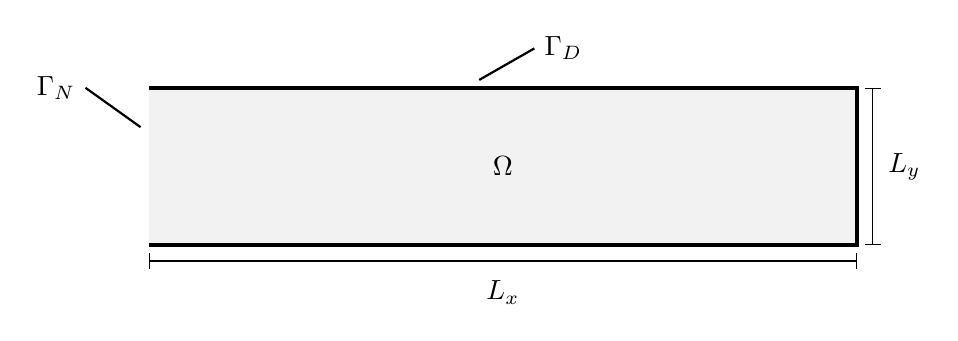
\begin{tikzpicture}
    \fill[black!5!white] (0, 0) rectangle (9, 2);
    \draw[ultra thick] (0, 0) to (9, 0) to (9, 2) to (0, 2);
    \draw[thick] (-0.8, 2) node[left] {$\Gamma_N$} to (-0.1, 1.5);
    \draw[thick] (4.9, 2.5) node[right] {$\Gamma_D$} to (4.2, 2.1);
    \draw[|-|] (0, -0.2) to (9, -0.2);
    \draw[|-|] (9.2, 0) to (9.2, 2);
    \node at (4.5, -0.6) {$L_x$};
    \node at (9.6, 1) {$L_y$};
    \node at (4.5, 1) {$\Omega$};
\end{tikzpicture}

    \caption{The rectangular resonant cavity is a medium $\Omega$ enclosed
    by a perfectly conducting boundary $\Gamma_D$ and an inlet $\Gamma_N$
    chosen to coincide with the rectangle's edge at $x=0$ for the experiments in this
    section.}
    \label{fig:rectangular_cavity}
\end{figure}

For simplicity, I set $\epsilon=\mu=1$. A uniform grid with 101 subdivisions in
the $x$- and 21 in the $y$-direction whose cells are again subdivided by their
diagonals was used to generate a highly symmetric triangular mesh that allows for 4365 degrees of freedom.
The system is forced from the inlet at $x=0$ with $g_z(y) = sin(\pi y / L_y)$.

% Exploratory plots
\subsubsection{Exploration of the problem}
\label{subsubsec:exploration}

To give the reader an impression of what the solution $\mathbf{u}_z$ to this problem
looks like, I plot the \acrshort{FEM}-solution at the first and sixth numerical resonant
frequencies in Figures \ref{fig:rectangular-cavity-mode1} and \ref{fig:rectangular-cavity-mode5}
respectively. Notice that I type its variable in bold, since it is a large vector with the values
for each of the \acrshort{DOF}s as its components.

\begin{figure}[ht]
    \centering
    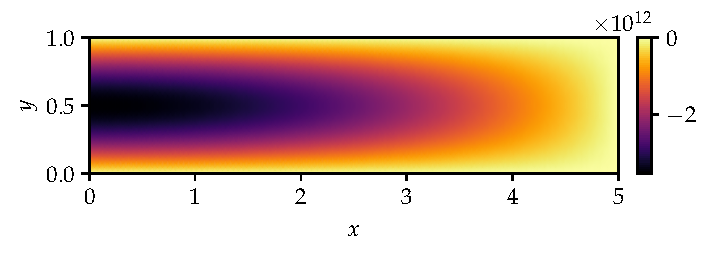
\includegraphics{plots/rectangular_cavity_mode1.pdf}
    \caption{The solution $\mathbf{u}_z$ obtained with the \acrshort{FEM} at the
    first numerical resonant frequency of the cavity. Observe how at
    every perfectly conducting boundary $\Gamma_D$ (cf. Figure
    \ref{fig:rectangular_cavity}) the solution gradually goes to zero, as I imposed.}
    \label{fig:rectangular-cavity-mode1}
\end{figure}

\begin{figure}[ht]
    \centering
    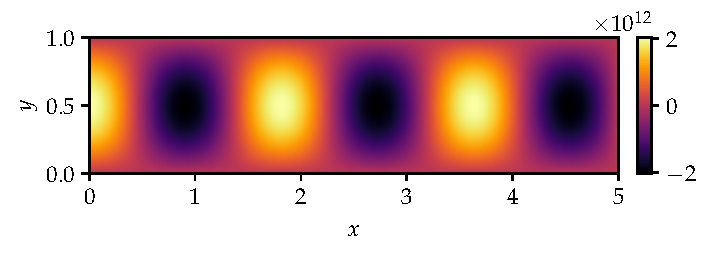
\includegraphics{plots/rectangular_cavity_mode5.pdf}
    \caption{The solution $\mathbf{u}_z$ obtained with the \acrshort{FEM} at the
    sixth numerical resonant frequency of the cavity.}
    \label{fig:rectangular-cavity-mode5}
\end{figure}

% Rational interpolation demonstration
I now study the \acrshort{gMRI} for the quantity $u_z$.
Algorithm \ref{alg:gMRI} is performed with a tolerance of $\tau = 10^{-2}$.
The candidate support points $\Omega_{\mathrm{test}}$
are 1000 uniformly spaced points in $\omega = [3, 5]$. The \acrshort{FEM} solution $u_z$
is computed and the \acrshort{gMRI} surrogate $\tilde{u}_z$ evaluated at all points in $\Omega_{\mathrm{test}}$,
and the $||\cdot||_M$-norm for both is plotted in Figure \ref{fig:rectangular-cavity-norms}. 

\begin{figure}[ht]
    \centering
    %% Creator: Matplotlib, PGF backend
%%
%% To include the figure in your LaTeX document, write
%%   \input{<filename>.pgf}
%%
%% Make sure the required packages are loaded in your preamble
%%   \usepackage{pgf}
%%
%% Also ensure that all the required font packages are loaded; for instance,
%% the lmodern package is sometimes necessary when using math font.
%%   \usepackage{lmodern}
%%
%% Figures using additional raster images can only be included by \input if
%% they are in the same directory as the main LaTeX file. For loading figures
%% from other directories you can use the `import` package
%%   \usepackage{import}
%%
%% and then include the figures with
%%   \import{<path to file>}{<filename>.pgf}
%%
%% Matplotlib used the following preamble
%%   \usepackage{fontspec}
%%   \setmainfont{DejaVuSans.ttf}[Path=\detokenize{C:/Users/Fabio/Anaconda3/Lib/site-packages/matplotlib/mpl-data/fonts/ttf/}]
%%   \setsansfont{DejaVuSans.ttf}[Path=\detokenize{C:/Users/Fabio/Anaconda3/Lib/site-packages/matplotlib/mpl-data/fonts/ttf/}]
%%   \setmonofont{DejaVuSansMono.ttf}[Path=\detokenize{C:/Users/Fabio/Anaconda3/Lib/site-packages/matplotlib/mpl-data/fonts/ttf/}]
%%
\begingroup%
\makeatletter%
\begin{pgfpicture}%
\pgfpathrectangle{\pgfpointorigin}{\pgfqpoint{5.180059in}{3.668486in}}%
\pgfusepath{use as bounding box, clip}%
\begin{pgfscope}%
\pgfsetbuttcap%
\pgfsetmiterjoin%
\pgfsetlinewidth{0.000000pt}%
\definecolor{currentstroke}{rgb}{1.000000,1.000000,1.000000}%
\pgfsetstrokecolor{currentstroke}%
\pgfsetstrokeopacity{0.000000}%
\pgfsetdash{}{0pt}%
\pgfpathmoveto{\pgfqpoint{0.000000in}{0.000000in}}%
\pgfpathlineto{\pgfqpoint{5.180059in}{0.000000in}}%
\pgfpathlineto{\pgfqpoint{5.180059in}{3.668486in}}%
\pgfpathlineto{\pgfqpoint{0.000000in}{3.668486in}}%
\pgfpathlineto{\pgfqpoint{0.000000in}{0.000000in}}%
\pgfpathclose%
\pgfusepath{}%
\end{pgfscope}%
\begin{pgfscope}%
\pgfsetbuttcap%
\pgfsetmiterjoin%
\definecolor{currentfill}{rgb}{1.000000,1.000000,1.000000}%
\pgfsetfillcolor{currentfill}%
\pgfsetlinewidth{0.000000pt}%
\definecolor{currentstroke}{rgb}{0.000000,0.000000,0.000000}%
\pgfsetstrokecolor{currentstroke}%
\pgfsetstrokeopacity{0.000000}%
\pgfsetdash{}{0pt}%
\pgfpathmoveto{\pgfqpoint{0.643624in}{2.195759in}}%
\pgfpathlineto{\pgfqpoint{4.944874in}{2.195759in}}%
\pgfpathlineto{\pgfqpoint{4.944874in}{3.568486in}}%
\pgfpathlineto{\pgfqpoint{0.643624in}{3.568486in}}%
\pgfpathlineto{\pgfqpoint{0.643624in}{2.195759in}}%
\pgfpathclose%
\pgfusepath{fill}%
\end{pgfscope}%
\begin{pgfscope}%
\pgfsetbuttcap%
\pgfsetroundjoin%
\definecolor{currentfill}{rgb}{0.000000,0.000000,0.000000}%
\pgfsetfillcolor{currentfill}%
\pgfsetlinewidth{0.803000pt}%
\definecolor{currentstroke}{rgb}{0.000000,0.000000,0.000000}%
\pgfsetstrokecolor{currentstroke}%
\pgfsetdash{}{0pt}%
\pgfsys@defobject{currentmarker}{\pgfqpoint{0.000000in}{-0.048611in}}{\pgfqpoint{0.000000in}{0.000000in}}{%
\pgfpathmoveto{\pgfqpoint{0.000000in}{0.000000in}}%
\pgfpathlineto{\pgfqpoint{0.000000in}{-0.048611in}}%
\pgfusepath{stroke,fill}%
}%
\begin{pgfscope}%
\pgfsys@transformshift{0.643624in}{2.195759in}%
\pgfsys@useobject{currentmarker}{}%
\end{pgfscope}%
\end{pgfscope}%
\begin{pgfscope}%
\pgfsetbuttcap%
\pgfsetroundjoin%
\definecolor{currentfill}{rgb}{0.000000,0.000000,0.000000}%
\pgfsetfillcolor{currentfill}%
\pgfsetlinewidth{0.803000pt}%
\definecolor{currentstroke}{rgb}{0.000000,0.000000,0.000000}%
\pgfsetstrokecolor{currentstroke}%
\pgfsetdash{}{0pt}%
\pgfsys@defobject{currentmarker}{\pgfqpoint{0.000000in}{-0.048611in}}{\pgfqpoint{0.000000in}{0.000000in}}{%
\pgfpathmoveto{\pgfqpoint{0.000000in}{0.000000in}}%
\pgfpathlineto{\pgfqpoint{0.000000in}{-0.048611in}}%
\pgfusepath{stroke,fill}%
}%
\begin{pgfscope}%
\pgfsys@transformshift{1.181280in}{2.195759in}%
\pgfsys@useobject{currentmarker}{}%
\end{pgfscope}%
\end{pgfscope}%
\begin{pgfscope}%
\pgfsetbuttcap%
\pgfsetroundjoin%
\definecolor{currentfill}{rgb}{0.000000,0.000000,0.000000}%
\pgfsetfillcolor{currentfill}%
\pgfsetlinewidth{0.803000pt}%
\definecolor{currentstroke}{rgb}{0.000000,0.000000,0.000000}%
\pgfsetstrokecolor{currentstroke}%
\pgfsetdash{}{0pt}%
\pgfsys@defobject{currentmarker}{\pgfqpoint{0.000000in}{-0.048611in}}{\pgfqpoint{0.000000in}{0.000000in}}{%
\pgfpathmoveto{\pgfqpoint{0.000000in}{0.000000in}}%
\pgfpathlineto{\pgfqpoint{0.000000in}{-0.048611in}}%
\pgfusepath{stroke,fill}%
}%
\begin{pgfscope}%
\pgfsys@transformshift{1.718936in}{2.195759in}%
\pgfsys@useobject{currentmarker}{}%
\end{pgfscope}%
\end{pgfscope}%
\begin{pgfscope}%
\pgfsetbuttcap%
\pgfsetroundjoin%
\definecolor{currentfill}{rgb}{0.000000,0.000000,0.000000}%
\pgfsetfillcolor{currentfill}%
\pgfsetlinewidth{0.803000pt}%
\definecolor{currentstroke}{rgb}{0.000000,0.000000,0.000000}%
\pgfsetstrokecolor{currentstroke}%
\pgfsetdash{}{0pt}%
\pgfsys@defobject{currentmarker}{\pgfqpoint{0.000000in}{-0.048611in}}{\pgfqpoint{0.000000in}{0.000000in}}{%
\pgfpathmoveto{\pgfqpoint{0.000000in}{0.000000in}}%
\pgfpathlineto{\pgfqpoint{0.000000in}{-0.048611in}}%
\pgfusepath{stroke,fill}%
}%
\begin{pgfscope}%
\pgfsys@transformshift{2.256593in}{2.195759in}%
\pgfsys@useobject{currentmarker}{}%
\end{pgfscope}%
\end{pgfscope}%
\begin{pgfscope}%
\pgfsetbuttcap%
\pgfsetroundjoin%
\definecolor{currentfill}{rgb}{0.000000,0.000000,0.000000}%
\pgfsetfillcolor{currentfill}%
\pgfsetlinewidth{0.803000pt}%
\definecolor{currentstroke}{rgb}{0.000000,0.000000,0.000000}%
\pgfsetstrokecolor{currentstroke}%
\pgfsetdash{}{0pt}%
\pgfsys@defobject{currentmarker}{\pgfqpoint{0.000000in}{-0.048611in}}{\pgfqpoint{0.000000in}{0.000000in}}{%
\pgfpathmoveto{\pgfqpoint{0.000000in}{0.000000in}}%
\pgfpathlineto{\pgfqpoint{0.000000in}{-0.048611in}}%
\pgfusepath{stroke,fill}%
}%
\begin{pgfscope}%
\pgfsys@transformshift{2.794249in}{2.195759in}%
\pgfsys@useobject{currentmarker}{}%
\end{pgfscope}%
\end{pgfscope}%
\begin{pgfscope}%
\pgfsetbuttcap%
\pgfsetroundjoin%
\definecolor{currentfill}{rgb}{0.000000,0.000000,0.000000}%
\pgfsetfillcolor{currentfill}%
\pgfsetlinewidth{0.803000pt}%
\definecolor{currentstroke}{rgb}{0.000000,0.000000,0.000000}%
\pgfsetstrokecolor{currentstroke}%
\pgfsetdash{}{0pt}%
\pgfsys@defobject{currentmarker}{\pgfqpoint{0.000000in}{-0.048611in}}{\pgfqpoint{0.000000in}{0.000000in}}{%
\pgfpathmoveto{\pgfqpoint{0.000000in}{0.000000in}}%
\pgfpathlineto{\pgfqpoint{0.000000in}{-0.048611in}}%
\pgfusepath{stroke,fill}%
}%
\begin{pgfscope}%
\pgfsys@transformshift{3.331905in}{2.195759in}%
\pgfsys@useobject{currentmarker}{}%
\end{pgfscope}%
\end{pgfscope}%
\begin{pgfscope}%
\pgfsetbuttcap%
\pgfsetroundjoin%
\definecolor{currentfill}{rgb}{0.000000,0.000000,0.000000}%
\pgfsetfillcolor{currentfill}%
\pgfsetlinewidth{0.803000pt}%
\definecolor{currentstroke}{rgb}{0.000000,0.000000,0.000000}%
\pgfsetstrokecolor{currentstroke}%
\pgfsetdash{}{0pt}%
\pgfsys@defobject{currentmarker}{\pgfqpoint{0.000000in}{-0.048611in}}{\pgfqpoint{0.000000in}{0.000000in}}{%
\pgfpathmoveto{\pgfqpoint{0.000000in}{0.000000in}}%
\pgfpathlineto{\pgfqpoint{0.000000in}{-0.048611in}}%
\pgfusepath{stroke,fill}%
}%
\begin{pgfscope}%
\pgfsys@transformshift{3.869561in}{2.195759in}%
\pgfsys@useobject{currentmarker}{}%
\end{pgfscope}%
\end{pgfscope}%
\begin{pgfscope}%
\pgfsetbuttcap%
\pgfsetroundjoin%
\definecolor{currentfill}{rgb}{0.000000,0.000000,0.000000}%
\pgfsetfillcolor{currentfill}%
\pgfsetlinewidth{0.803000pt}%
\definecolor{currentstroke}{rgb}{0.000000,0.000000,0.000000}%
\pgfsetstrokecolor{currentstroke}%
\pgfsetdash{}{0pt}%
\pgfsys@defobject{currentmarker}{\pgfqpoint{0.000000in}{-0.048611in}}{\pgfqpoint{0.000000in}{0.000000in}}{%
\pgfpathmoveto{\pgfqpoint{0.000000in}{0.000000in}}%
\pgfpathlineto{\pgfqpoint{0.000000in}{-0.048611in}}%
\pgfusepath{stroke,fill}%
}%
\begin{pgfscope}%
\pgfsys@transformshift{4.407218in}{2.195759in}%
\pgfsys@useobject{currentmarker}{}%
\end{pgfscope}%
\end{pgfscope}%
\begin{pgfscope}%
\pgfsetbuttcap%
\pgfsetroundjoin%
\definecolor{currentfill}{rgb}{0.000000,0.000000,0.000000}%
\pgfsetfillcolor{currentfill}%
\pgfsetlinewidth{0.803000pt}%
\definecolor{currentstroke}{rgb}{0.000000,0.000000,0.000000}%
\pgfsetstrokecolor{currentstroke}%
\pgfsetdash{}{0pt}%
\pgfsys@defobject{currentmarker}{\pgfqpoint{0.000000in}{-0.048611in}}{\pgfqpoint{0.000000in}{0.000000in}}{%
\pgfpathmoveto{\pgfqpoint{0.000000in}{0.000000in}}%
\pgfpathlineto{\pgfqpoint{0.000000in}{-0.048611in}}%
\pgfusepath{stroke,fill}%
}%
\begin{pgfscope}%
\pgfsys@transformshift{4.944874in}{2.195759in}%
\pgfsys@useobject{currentmarker}{}%
\end{pgfscope}%
\end{pgfscope}%
\begin{pgfscope}%
\pgfpathrectangle{\pgfqpoint{0.643624in}{2.195759in}}{\pgfqpoint{4.301250in}{1.372727in}}%
\pgfusepath{clip}%
\pgfsetrectcap%
\pgfsetroundjoin%
\pgfsetlinewidth{0.803000pt}%
\definecolor{currentstroke}{rgb}{0.690196,0.690196,0.690196}%
\pgfsetstrokecolor{currentstroke}%
\pgfsetdash{}{0pt}%
\pgfpathmoveto{\pgfqpoint{0.643624in}{2.778814in}}%
\pgfpathlineto{\pgfqpoint{4.944874in}{2.778814in}}%
\pgfusepath{stroke}%
\end{pgfscope}%
\begin{pgfscope}%
\pgfsetbuttcap%
\pgfsetroundjoin%
\definecolor{currentfill}{rgb}{0.000000,0.000000,0.000000}%
\pgfsetfillcolor{currentfill}%
\pgfsetlinewidth{0.803000pt}%
\definecolor{currentstroke}{rgb}{0.000000,0.000000,0.000000}%
\pgfsetstrokecolor{currentstroke}%
\pgfsetdash{}{0pt}%
\pgfsys@defobject{currentmarker}{\pgfqpoint{-0.048611in}{0.000000in}}{\pgfqpoint{-0.000000in}{0.000000in}}{%
\pgfpathmoveto{\pgfqpoint{-0.000000in}{0.000000in}}%
\pgfpathlineto{\pgfqpoint{-0.048611in}{0.000000in}}%
\pgfusepath{stroke,fill}%
}%
\begin{pgfscope}%
\pgfsys@transformshift{0.643624in}{2.778814in}%
\pgfsys@useobject{currentmarker}{}%
\end{pgfscope}%
\end{pgfscope}%
\begin{pgfscope}%
\definecolor{textcolor}{rgb}{0.000000,0.000000,0.000000}%
\pgfsetstrokecolor{textcolor}%
\pgfsetfillcolor{textcolor}%
\pgftext[x=0.328345in, y=2.720777in, left, base]{\color{textcolor}\rmfamily\fontsize{11.000000}{13.200000}\selectfont \(\displaystyle {10^{1}}\)}%
\end{pgfscope}%
\begin{pgfscope}%
\pgfpathrectangle{\pgfqpoint{0.643624in}{2.195759in}}{\pgfqpoint{4.301250in}{1.372727in}}%
\pgfusepath{clip}%
\pgfsetrectcap%
\pgfsetroundjoin%
\pgfsetlinewidth{0.803000pt}%
\definecolor{currentstroke}{rgb}{0.690196,0.690196,0.690196}%
\pgfsetstrokecolor{currentstroke}%
\pgfsetdash{}{0pt}%
\pgfpathmoveto{\pgfqpoint{0.643624in}{3.465178in}}%
\pgfpathlineto{\pgfqpoint{4.944874in}{3.465178in}}%
\pgfusepath{stroke}%
\end{pgfscope}%
\begin{pgfscope}%
\pgfsetbuttcap%
\pgfsetroundjoin%
\definecolor{currentfill}{rgb}{0.000000,0.000000,0.000000}%
\pgfsetfillcolor{currentfill}%
\pgfsetlinewidth{0.803000pt}%
\definecolor{currentstroke}{rgb}{0.000000,0.000000,0.000000}%
\pgfsetstrokecolor{currentstroke}%
\pgfsetdash{}{0pt}%
\pgfsys@defobject{currentmarker}{\pgfqpoint{-0.048611in}{0.000000in}}{\pgfqpoint{-0.000000in}{0.000000in}}{%
\pgfpathmoveto{\pgfqpoint{-0.000000in}{0.000000in}}%
\pgfpathlineto{\pgfqpoint{-0.048611in}{0.000000in}}%
\pgfusepath{stroke,fill}%
}%
\begin{pgfscope}%
\pgfsys@transformshift{0.643624in}{3.465178in}%
\pgfsys@useobject{currentmarker}{}%
\end{pgfscope}%
\end{pgfscope}%
\begin{pgfscope}%
\definecolor{textcolor}{rgb}{0.000000,0.000000,0.000000}%
\pgfsetstrokecolor{textcolor}%
\pgfsetfillcolor{textcolor}%
\pgftext[x=0.328345in, y=3.407140in, left, base]{\color{textcolor}\rmfamily\fontsize{11.000000}{13.200000}\selectfont \(\displaystyle {10^{3}}\)}%
\end{pgfscope}%
\begin{pgfscope}%
\definecolor{textcolor}{rgb}{0.000000,0.000000,0.000000}%
\pgfsetstrokecolor{textcolor}%
\pgfsetfillcolor{textcolor}%
\pgftext[x=0.272790in,y=2.882122in,,bottom,rotate=90.000000]{\color{textcolor}\rmfamily\fontsize{11.000000}{13.200000}\selectfont \(\displaystyle ||u(\omega)||_{L_2(\Omega)}\)}%
\end{pgfscope}%
\begin{pgfscope}%
\pgfpathrectangle{\pgfqpoint{0.643624in}{2.195759in}}{\pgfqpoint{4.301250in}{1.372727in}}%
\pgfusepath{clip}%
\pgfsetrectcap%
\pgfsetroundjoin%
\pgfsetlinewidth{1.505625pt}%
\definecolor{currentstroke}{rgb}{0.001462,0.000466,0.013866}%
\pgfsetstrokecolor{currentstroke}%
\pgfsetdash{}{0pt}%
\pgfpathmoveto{\pgfqpoint{0.643624in}{2.345949in}}%
\pgfpathlineto{\pgfqpoint{0.695291in}{2.365853in}}%
\pgfpathlineto{\pgfqpoint{0.738346in}{2.385738in}}%
\pgfpathlineto{\pgfqpoint{0.772791in}{2.404671in}}%
\pgfpathlineto{\pgfqpoint{0.802929in}{2.424295in}}%
\pgfpathlineto{\pgfqpoint{0.828763in}{2.444241in}}%
\pgfpathlineto{\pgfqpoint{0.854596in}{2.468223in}}%
\pgfpathlineto{\pgfqpoint{0.876124in}{2.492587in}}%
\pgfpathlineto{\pgfqpoint{0.893346in}{2.516191in}}%
\pgfpathlineto{\pgfqpoint{0.910568in}{2.545108in}}%
\pgfpathlineto{\pgfqpoint{0.923485in}{2.571883in}}%
\pgfpathlineto{\pgfqpoint{0.936402in}{2.605265in}}%
\pgfpathlineto{\pgfqpoint{0.949318in}{2.649267in}}%
\pgfpathlineto{\pgfqpoint{0.957929in}{2.688624in}}%
\pgfpathlineto{\pgfqpoint{0.966541in}{2.742859in}}%
\pgfpathlineto{\pgfqpoint{0.975152in}{2.829861in}}%
\pgfpathlineto{\pgfqpoint{0.979457in}{2.905503in}}%
\pgfpathlineto{\pgfqpoint{0.983763in}{3.067348in}}%
\pgfpathlineto{\pgfqpoint{0.988068in}{3.072782in}}%
\pgfpathlineto{\pgfqpoint{0.992374in}{2.907192in}}%
\pgfpathlineto{\pgfqpoint{1.000985in}{2.780538in}}%
\pgfpathlineto{\pgfqpoint{1.009596in}{2.713424in}}%
\pgfpathlineto{\pgfqpoint{1.018207in}{2.667808in}}%
\pgfpathlineto{\pgfqpoint{1.031124in}{2.619263in}}%
\pgfpathlineto{\pgfqpoint{1.044041in}{2.584374in}}%
\pgfpathlineto{\pgfqpoint{1.056957in}{2.558211in}}%
\pgfpathlineto{\pgfqpoint{1.069874in}{2.538484in}}%
\pgfpathlineto{\pgfqpoint{1.082791in}{2.524025in}}%
\pgfpathlineto{\pgfqpoint{1.095707in}{2.514222in}}%
\pgfpathlineto{\pgfqpoint{1.108624in}{2.508766in}}%
\pgfpathlineto{\pgfqpoint{1.121541in}{2.507520in}}%
\pgfpathlineto{\pgfqpoint{1.134457in}{2.510467in}}%
\pgfpathlineto{\pgfqpoint{1.147374in}{2.517693in}}%
\pgfpathlineto{\pgfqpoint{1.160291in}{2.529429in}}%
\pgfpathlineto{\pgfqpoint{1.173207in}{2.546143in}}%
\pgfpathlineto{\pgfqpoint{1.186124in}{2.568725in}}%
\pgfpathlineto{\pgfqpoint{1.199041in}{2.598881in}}%
\pgfpathlineto{\pgfqpoint{1.211957in}{2.640101in}}%
\pgfpathlineto{\pgfqpoint{1.220568in}{2.677388in}}%
\pgfpathlineto{\pgfqpoint{1.229179in}{2.728552in}}%
\pgfpathlineto{\pgfqpoint{1.237791in}{2.808591in}}%
\pgfpathlineto{\pgfqpoint{1.242096in}{2.874617in}}%
\pgfpathlineto{\pgfqpoint{1.246402in}{2.996603in}}%
\pgfpathlineto{\pgfqpoint{1.250707in}{3.192332in}}%
\pgfpathlineto{\pgfqpoint{1.255013in}{2.932406in}}%
\pgfpathlineto{\pgfqpoint{1.259318in}{2.842774in}}%
\pgfpathlineto{\pgfqpoint{1.267929in}{2.747005in}}%
\pgfpathlineto{\pgfqpoint{1.276541in}{2.689486in}}%
\pgfpathlineto{\pgfqpoint{1.285152in}{2.648430in}}%
\pgfpathlineto{\pgfqpoint{1.298068in}{2.603093in}}%
\pgfpathlineto{\pgfqpoint{1.310985in}{2.569109in}}%
\pgfpathlineto{\pgfqpoint{1.328207in}{2.534354in}}%
\pgfpathlineto{\pgfqpoint{1.345429in}{2.507410in}}%
\pgfpathlineto{\pgfqpoint{1.362652in}{2.485828in}}%
\pgfpathlineto{\pgfqpoint{1.384179in}{2.464349in}}%
\pgfpathlineto{\pgfqpoint{1.405707in}{2.447574in}}%
\pgfpathlineto{\pgfqpoint{1.427235in}{2.434619in}}%
\pgfpathlineto{\pgfqpoint{1.448763in}{2.424977in}}%
\pgfpathlineto{\pgfqpoint{1.470291in}{2.418370in}}%
\pgfpathlineto{\pgfqpoint{1.491818in}{2.414675in}}%
\pgfpathlineto{\pgfqpoint{1.513346in}{2.413876in}}%
\pgfpathlineto{\pgfqpoint{1.534874in}{2.416045in}}%
\pgfpathlineto{\pgfqpoint{1.556402in}{2.421342in}}%
\pgfpathlineto{\pgfqpoint{1.577929in}{2.430022in}}%
\pgfpathlineto{\pgfqpoint{1.599457in}{2.442482in}}%
\pgfpathlineto{\pgfqpoint{1.616679in}{2.455579in}}%
\pgfpathlineto{\pgfqpoint{1.633902in}{2.471972in}}%
\pgfpathlineto{\pgfqpoint{1.651124in}{2.492410in}}%
\pgfpathlineto{\pgfqpoint{1.668346in}{2.518107in}}%
\pgfpathlineto{\pgfqpoint{1.681263in}{2.542052in}}%
\pgfpathlineto{\pgfqpoint{1.694179in}{2.571668in}}%
\pgfpathlineto{\pgfqpoint{1.707096in}{2.609768in}}%
\pgfpathlineto{\pgfqpoint{1.715707in}{2.642544in}}%
\pgfpathlineto{\pgfqpoint{1.724318in}{2.685113in}}%
\pgfpathlineto{\pgfqpoint{1.732929in}{2.745489in}}%
\pgfpathlineto{\pgfqpoint{1.737235in}{2.788521in}}%
\pgfpathlineto{\pgfqpoint{1.741541in}{2.849420in}}%
\pgfpathlineto{\pgfqpoint{1.745846in}{2.954376in}}%
\pgfpathlineto{\pgfqpoint{1.750152in}{3.514627in}}%
\pgfpathlineto{\pgfqpoint{1.754457in}{2.947504in}}%
\pgfpathlineto{\pgfqpoint{1.758763in}{2.845857in}}%
\pgfpathlineto{\pgfqpoint{1.767374in}{2.743445in}}%
\pgfpathlineto{\pgfqpoint{1.775985in}{2.683438in}}%
\pgfpathlineto{\pgfqpoint{1.784596in}{2.640928in}}%
\pgfpathlineto{\pgfqpoint{1.797513in}{2.594069in}}%
\pgfpathlineto{\pgfqpoint{1.810429in}{2.558851in}}%
\pgfpathlineto{\pgfqpoint{1.827652in}{2.522581in}}%
\pgfpathlineto{\pgfqpoint{1.844874in}{2.494115in}}%
\pgfpathlineto{\pgfqpoint{1.862096in}{2.470915in}}%
\pgfpathlineto{\pgfqpoint{1.883624in}{2.447181in}}%
\pgfpathlineto{\pgfqpoint{1.905152in}{2.427778in}}%
\pgfpathlineto{\pgfqpoint{1.930985in}{2.408812in}}%
\pgfpathlineto{\pgfqpoint{1.956818in}{2.393553in}}%
\pgfpathlineto{\pgfqpoint{1.986957in}{2.379553in}}%
\pgfpathlineto{\pgfqpoint{2.017096in}{2.369037in}}%
\pgfpathlineto{\pgfqpoint{2.047235in}{2.361628in}}%
\pgfpathlineto{\pgfqpoint{2.077374in}{2.357131in}}%
\pgfpathlineto{\pgfqpoint{2.107513in}{2.355481in}}%
\pgfpathlineto{\pgfqpoint{2.137652in}{2.356721in}}%
\pgfpathlineto{\pgfqpoint{2.167791in}{2.360988in}}%
\pgfpathlineto{\pgfqpoint{2.197929in}{2.368530in}}%
\pgfpathlineto{\pgfqpoint{2.223763in}{2.377888in}}%
\pgfpathlineto{\pgfqpoint{2.249596in}{2.390293in}}%
\pgfpathlineto{\pgfqpoint{2.275429in}{2.406284in}}%
\pgfpathlineto{\pgfqpoint{2.296957in}{2.422935in}}%
\pgfpathlineto{\pgfqpoint{2.318485in}{2.443387in}}%
\pgfpathlineto{\pgfqpoint{2.340013in}{2.468824in}}%
\pgfpathlineto{\pgfqpoint{2.357235in}{2.494084in}}%
\pgfpathlineto{\pgfqpoint{2.374457in}{2.525627in}}%
\pgfpathlineto{\pgfqpoint{2.387374in}{2.555346in}}%
\pgfpathlineto{\pgfqpoint{2.400291in}{2.593149in}}%
\pgfpathlineto{\pgfqpoint{2.408902in}{2.625369in}}%
\pgfpathlineto{\pgfqpoint{2.417513in}{2.666833in}}%
\pgfpathlineto{\pgfqpoint{2.426124in}{2.724829in}}%
\pgfpathlineto{\pgfqpoint{2.430429in}{2.765444in}}%
\pgfpathlineto{\pgfqpoint{2.434735in}{2.821555in}}%
\pgfpathlineto{\pgfqpoint{2.439041in}{2.912757in}}%
\pgfpathlineto{\pgfqpoint{2.443346in}{3.190334in}}%
\pgfpathlineto{\pgfqpoint{2.447652in}{2.968084in}}%
\pgfpathlineto{\pgfqpoint{2.451957in}{2.848857in}}%
\pgfpathlineto{\pgfqpoint{2.460568in}{2.738197in}}%
\pgfpathlineto{\pgfqpoint{2.469179in}{2.675453in}}%
\pgfpathlineto{\pgfqpoint{2.477791in}{2.631520in}}%
\pgfpathlineto{\pgfqpoint{2.490707in}{2.583379in}}%
\pgfpathlineto{\pgfqpoint{2.503624in}{2.547287in}}%
\pgfpathlineto{\pgfqpoint{2.520846in}{2.510093in}}%
\pgfpathlineto{\pgfqpoint{2.538068in}{2.480804in}}%
\pgfpathlineto{\pgfqpoint{2.559596in}{2.451442in}}%
\pgfpathlineto{\pgfqpoint{2.581124in}{2.427647in}}%
\pgfpathlineto{\pgfqpoint{2.606957in}{2.404305in}}%
\pgfpathlineto{\pgfqpoint{2.632791in}{2.385183in}}%
\pgfpathlineto{\pgfqpoint{2.662929in}{2.366933in}}%
\pgfpathlineto{\pgfqpoint{2.693068in}{2.352148in}}%
\pgfpathlineto{\pgfqpoint{2.727513in}{2.338714in}}%
\pgfpathlineto{\pgfqpoint{2.761957in}{2.328425in}}%
\pgfpathlineto{\pgfqpoint{2.800707in}{2.320174in}}%
\pgfpathlineto{\pgfqpoint{2.839457in}{2.315180in}}%
\pgfpathlineto{\pgfqpoint{2.878207in}{2.313337in}}%
\pgfpathlineto{\pgfqpoint{2.916957in}{2.314677in}}%
\pgfpathlineto{\pgfqpoint{2.955707in}{2.319359in}}%
\pgfpathlineto{\pgfqpoint{2.990152in}{2.326566in}}%
\pgfpathlineto{\pgfqpoint{3.024596in}{2.336982in}}%
\pgfpathlineto{\pgfqpoint{3.054735in}{2.349118in}}%
\pgfpathlineto{\pgfqpoint{3.084874in}{2.364598in}}%
\pgfpathlineto{\pgfqpoint{3.110707in}{2.381099in}}%
\pgfpathlineto{\pgfqpoint{3.136541in}{2.401352in}}%
\pgfpathlineto{\pgfqpoint{3.158068in}{2.421922in}}%
\pgfpathlineto{\pgfqpoint{3.179596in}{2.446986in}}%
\pgfpathlineto{\pgfqpoint{3.196818in}{2.471456in}}%
\pgfpathlineto{\pgfqpoint{3.214041in}{2.501530in}}%
\pgfpathlineto{\pgfqpoint{3.226957in}{2.529402in}}%
\pgfpathlineto{\pgfqpoint{3.239874in}{2.564172in}}%
\pgfpathlineto{\pgfqpoint{3.252791in}{2.610106in}}%
\pgfpathlineto{\pgfqpoint{3.261402in}{2.651428in}}%
\pgfpathlineto{\pgfqpoint{3.270013in}{2.709063in}}%
\pgfpathlineto{\pgfqpoint{3.274318in}{2.749300in}}%
\pgfpathlineto{\pgfqpoint{3.278624in}{2.804669in}}%
\pgfpathlineto{\pgfqpoint{3.282929in}{2.893863in}}%
\pgfpathlineto{\pgfqpoint{3.287235in}{3.149362in}}%
\pgfpathlineto{\pgfqpoint{3.295846in}{2.837376in}}%
\pgfpathlineto{\pgfqpoint{3.304457in}{2.725139in}}%
\pgfpathlineto{\pgfqpoint{3.313068in}{2.661882in}}%
\pgfpathlineto{\pgfqpoint{3.321679in}{2.617671in}}%
\pgfpathlineto{\pgfqpoint{3.334596in}{2.569254in}}%
\pgfpathlineto{\pgfqpoint{3.347513in}{2.532941in}}%
\pgfpathlineto{\pgfqpoint{3.364735in}{2.495470in}}%
\pgfpathlineto{\pgfqpoint{3.381957in}{2.465895in}}%
\pgfpathlineto{\pgfqpoint{3.403485in}{2.436143in}}%
\pgfpathlineto{\pgfqpoint{3.425013in}{2.411914in}}%
\pgfpathlineto{\pgfqpoint{3.450846in}{2.387986in}}%
\pgfpathlineto{\pgfqpoint{3.476679in}{2.368200in}}%
\pgfpathlineto{\pgfqpoint{3.506818in}{2.349065in}}%
\pgfpathlineto{\pgfqpoint{3.541263in}{2.331232in}}%
\pgfpathlineto{\pgfqpoint{3.575707in}{2.316827in}}%
\pgfpathlineto{\pgfqpoint{3.614457in}{2.303988in}}%
\pgfpathlineto{\pgfqpoint{3.653207in}{2.294203in}}%
\pgfpathlineto{\pgfqpoint{3.696263in}{2.286513in}}%
\pgfpathlineto{\pgfqpoint{3.739318in}{2.281934in}}%
\pgfpathlineto{\pgfqpoint{3.782374in}{2.280367in}}%
\pgfpathlineto{\pgfqpoint{3.825429in}{2.281840in}}%
\pgfpathlineto{\pgfqpoint{3.868485in}{2.286503in}}%
\pgfpathlineto{\pgfqpoint{3.907235in}{2.293658in}}%
\pgfpathlineto{\pgfqpoint{3.945985in}{2.303950in}}%
\pgfpathlineto{\pgfqpoint{3.980429in}{2.316127in}}%
\pgfpathlineto{\pgfqpoint{4.014874in}{2.331691in}}%
\pgfpathlineto{\pgfqpoint{4.045013in}{2.348702in}}%
\pgfpathlineto{\pgfqpoint{4.070846in}{2.366437in}}%
\pgfpathlineto{\pgfqpoint{4.096679in}{2.387907in}}%
\pgfpathlineto{\pgfqpoint{4.118207in}{2.409540in}}%
\pgfpathlineto{\pgfqpoint{4.139735in}{2.435805in}}%
\pgfpathlineto{\pgfqpoint{4.156957in}{2.461452in}}%
\pgfpathlineto{\pgfqpoint{4.174179in}{2.493082in}}%
\pgfpathlineto{\pgfqpoint{4.187096in}{2.522596in}}%
\pgfpathlineto{\pgfqpoint{4.200013in}{2.559816in}}%
\pgfpathlineto{\pgfqpoint{4.212929in}{2.609968in}}%
\pgfpathlineto{\pgfqpoint{4.221541in}{2.656456in}}%
\pgfpathlineto{\pgfqpoint{4.230152in}{2.724629in}}%
\pgfpathlineto{\pgfqpoint{4.234457in}{2.775775in}}%
\pgfpathlineto{\pgfqpoint{4.238763in}{2.854354in}}%
\pgfpathlineto{\pgfqpoint{4.243068in}{3.031187in}}%
\pgfpathlineto{\pgfqpoint{4.247374in}{2.994786in}}%
\pgfpathlineto{\pgfqpoint{4.251679in}{2.842190in}}%
\pgfpathlineto{\pgfqpoint{4.260291in}{2.719238in}}%
\pgfpathlineto{\pgfqpoint{4.268902in}{2.652818in}}%
\pgfpathlineto{\pgfqpoint{4.277513in}{2.607078in}}%
\pgfpathlineto{\pgfqpoint{4.290429in}{2.557414in}}%
\pgfpathlineto{\pgfqpoint{4.303346in}{2.520367in}}%
\pgfpathlineto{\pgfqpoint{4.320568in}{2.482250in}}%
\pgfpathlineto{\pgfqpoint{4.337791in}{2.452206in}}%
\pgfpathlineto{\pgfqpoint{4.359318in}{2.421981in}}%
\pgfpathlineto{\pgfqpoint{4.380846in}{2.397334in}}%
\pgfpathlineto{\pgfqpoint{4.406679in}{2.372930in}}%
\pgfpathlineto{\pgfqpoint{4.432513in}{2.352665in}}%
\pgfpathlineto{\pgfqpoint{4.462652in}{2.332945in}}%
\pgfpathlineto{\pgfqpoint{4.497096in}{2.314387in}}%
\pgfpathlineto{\pgfqpoint{4.535846in}{2.297472in}}%
\pgfpathlineto{\pgfqpoint{4.574596in}{2.283940in}}%
\pgfpathlineto{\pgfqpoint{4.617652in}{2.272213in}}%
\pgfpathlineto{\pgfqpoint{4.660707in}{2.263514in}}%
\pgfpathlineto{\pgfqpoint{4.708068in}{2.257103in}}%
\pgfpathlineto{\pgfqpoint{4.755429in}{2.253811in}}%
\pgfpathlineto{\pgfqpoint{4.802791in}{2.253589in}}%
\pgfpathlineto{\pgfqpoint{4.850152in}{2.256511in}}%
\pgfpathlineto{\pgfqpoint{4.893207in}{2.262067in}}%
\pgfpathlineto{\pgfqpoint{4.936263in}{2.270658in}}%
\pgfpathlineto{\pgfqpoint{4.944874in}{2.272773in}}%
\pgfpathlineto{\pgfqpoint{4.944874in}{2.272773in}}%
\pgfusepath{stroke}%
\end{pgfscope}%
\begin{pgfscope}%
\pgfsetrectcap%
\pgfsetmiterjoin%
\pgfsetlinewidth{0.803000pt}%
\definecolor{currentstroke}{rgb}{0.000000,0.000000,0.000000}%
\pgfsetstrokecolor{currentstroke}%
\pgfsetdash{}{0pt}%
\pgfpathmoveto{\pgfqpoint{0.643624in}{2.195759in}}%
\pgfpathlineto{\pgfqpoint{0.643624in}{3.568486in}}%
\pgfusepath{stroke}%
\end{pgfscope}%
\begin{pgfscope}%
\pgfsetrectcap%
\pgfsetmiterjoin%
\pgfsetlinewidth{0.803000pt}%
\definecolor{currentstroke}{rgb}{0.000000,0.000000,0.000000}%
\pgfsetstrokecolor{currentstroke}%
\pgfsetdash{}{0pt}%
\pgfpathmoveto{\pgfqpoint{4.944874in}{2.195759in}}%
\pgfpathlineto{\pgfqpoint{4.944874in}{3.568486in}}%
\pgfusepath{stroke}%
\end{pgfscope}%
\begin{pgfscope}%
\pgfsetrectcap%
\pgfsetmiterjoin%
\pgfsetlinewidth{0.803000pt}%
\definecolor{currentstroke}{rgb}{0.000000,0.000000,0.000000}%
\pgfsetstrokecolor{currentstroke}%
\pgfsetdash{}{0pt}%
\pgfpathmoveto{\pgfqpoint{0.643624in}{2.195759in}}%
\pgfpathlineto{\pgfqpoint{4.944874in}{2.195759in}}%
\pgfusepath{stroke}%
\end{pgfscope}%
\begin{pgfscope}%
\pgfsetrectcap%
\pgfsetmiterjoin%
\pgfsetlinewidth{0.803000pt}%
\definecolor{currentstroke}{rgb}{0.000000,0.000000,0.000000}%
\pgfsetstrokecolor{currentstroke}%
\pgfsetdash{}{0pt}%
\pgfpathmoveto{\pgfqpoint{0.643624in}{3.568486in}}%
\pgfpathlineto{\pgfqpoint{4.944874in}{3.568486in}}%
\pgfusepath{stroke}%
\end{pgfscope}%
\begin{pgfscope}%
\pgfsetbuttcap%
\pgfsetmiterjoin%
\definecolor{currentfill}{rgb}{1.000000,1.000000,1.000000}%
\pgfsetfillcolor{currentfill}%
\pgfsetlinewidth{0.000000pt}%
\definecolor{currentstroke}{rgb}{0.000000,0.000000,0.000000}%
\pgfsetstrokecolor{currentstroke}%
\pgfsetstrokeopacity{0.000000}%
\pgfsetdash{}{0pt}%
\pgfpathmoveto{\pgfqpoint{0.643624in}{0.823031in}}%
\pgfpathlineto{\pgfqpoint{4.944874in}{0.823031in}}%
\pgfpathlineto{\pgfqpoint{4.944874in}{2.195759in}}%
\pgfpathlineto{\pgfqpoint{0.643624in}{2.195759in}}%
\pgfpathlineto{\pgfqpoint{0.643624in}{0.823031in}}%
\pgfpathclose%
\pgfusepath{fill}%
\end{pgfscope}%
\begin{pgfscope}%
\pgfsetbuttcap%
\pgfsetroundjoin%
\definecolor{currentfill}{rgb}{0.000000,0.000000,0.000000}%
\pgfsetfillcolor{currentfill}%
\pgfsetlinewidth{0.803000pt}%
\definecolor{currentstroke}{rgb}{0.000000,0.000000,0.000000}%
\pgfsetstrokecolor{currentstroke}%
\pgfsetdash{}{0pt}%
\pgfsys@defobject{currentmarker}{\pgfqpoint{0.000000in}{-0.048611in}}{\pgfqpoint{0.000000in}{0.000000in}}{%
\pgfpathmoveto{\pgfqpoint{0.000000in}{0.000000in}}%
\pgfpathlineto{\pgfqpoint{0.000000in}{-0.048611in}}%
\pgfusepath{stroke,fill}%
}%
\begin{pgfscope}%
\pgfsys@transformshift{0.643624in}{0.823031in}%
\pgfsys@useobject{currentmarker}{}%
\end{pgfscope}%
\end{pgfscope}%
\begin{pgfscope}%
\pgfsetbuttcap%
\pgfsetroundjoin%
\definecolor{currentfill}{rgb}{0.000000,0.000000,0.000000}%
\pgfsetfillcolor{currentfill}%
\pgfsetlinewidth{0.803000pt}%
\definecolor{currentstroke}{rgb}{0.000000,0.000000,0.000000}%
\pgfsetstrokecolor{currentstroke}%
\pgfsetdash{}{0pt}%
\pgfsys@defobject{currentmarker}{\pgfqpoint{0.000000in}{-0.048611in}}{\pgfqpoint{0.000000in}{0.000000in}}{%
\pgfpathmoveto{\pgfqpoint{0.000000in}{0.000000in}}%
\pgfpathlineto{\pgfqpoint{0.000000in}{-0.048611in}}%
\pgfusepath{stroke,fill}%
}%
\begin{pgfscope}%
\pgfsys@transformshift{1.181280in}{0.823031in}%
\pgfsys@useobject{currentmarker}{}%
\end{pgfscope}%
\end{pgfscope}%
\begin{pgfscope}%
\pgfsetbuttcap%
\pgfsetroundjoin%
\definecolor{currentfill}{rgb}{0.000000,0.000000,0.000000}%
\pgfsetfillcolor{currentfill}%
\pgfsetlinewidth{0.803000pt}%
\definecolor{currentstroke}{rgb}{0.000000,0.000000,0.000000}%
\pgfsetstrokecolor{currentstroke}%
\pgfsetdash{}{0pt}%
\pgfsys@defobject{currentmarker}{\pgfqpoint{0.000000in}{-0.048611in}}{\pgfqpoint{0.000000in}{0.000000in}}{%
\pgfpathmoveto{\pgfqpoint{0.000000in}{0.000000in}}%
\pgfpathlineto{\pgfqpoint{0.000000in}{-0.048611in}}%
\pgfusepath{stroke,fill}%
}%
\begin{pgfscope}%
\pgfsys@transformshift{1.718936in}{0.823031in}%
\pgfsys@useobject{currentmarker}{}%
\end{pgfscope}%
\end{pgfscope}%
\begin{pgfscope}%
\pgfsetbuttcap%
\pgfsetroundjoin%
\definecolor{currentfill}{rgb}{0.000000,0.000000,0.000000}%
\pgfsetfillcolor{currentfill}%
\pgfsetlinewidth{0.803000pt}%
\definecolor{currentstroke}{rgb}{0.000000,0.000000,0.000000}%
\pgfsetstrokecolor{currentstroke}%
\pgfsetdash{}{0pt}%
\pgfsys@defobject{currentmarker}{\pgfqpoint{0.000000in}{-0.048611in}}{\pgfqpoint{0.000000in}{0.000000in}}{%
\pgfpathmoveto{\pgfqpoint{0.000000in}{0.000000in}}%
\pgfpathlineto{\pgfqpoint{0.000000in}{-0.048611in}}%
\pgfusepath{stroke,fill}%
}%
\begin{pgfscope}%
\pgfsys@transformshift{2.256593in}{0.823031in}%
\pgfsys@useobject{currentmarker}{}%
\end{pgfscope}%
\end{pgfscope}%
\begin{pgfscope}%
\pgfsetbuttcap%
\pgfsetroundjoin%
\definecolor{currentfill}{rgb}{0.000000,0.000000,0.000000}%
\pgfsetfillcolor{currentfill}%
\pgfsetlinewidth{0.803000pt}%
\definecolor{currentstroke}{rgb}{0.000000,0.000000,0.000000}%
\pgfsetstrokecolor{currentstroke}%
\pgfsetdash{}{0pt}%
\pgfsys@defobject{currentmarker}{\pgfqpoint{0.000000in}{-0.048611in}}{\pgfqpoint{0.000000in}{0.000000in}}{%
\pgfpathmoveto{\pgfqpoint{0.000000in}{0.000000in}}%
\pgfpathlineto{\pgfqpoint{0.000000in}{-0.048611in}}%
\pgfusepath{stroke,fill}%
}%
\begin{pgfscope}%
\pgfsys@transformshift{2.794249in}{0.823031in}%
\pgfsys@useobject{currentmarker}{}%
\end{pgfscope}%
\end{pgfscope}%
\begin{pgfscope}%
\pgfsetbuttcap%
\pgfsetroundjoin%
\definecolor{currentfill}{rgb}{0.000000,0.000000,0.000000}%
\pgfsetfillcolor{currentfill}%
\pgfsetlinewidth{0.803000pt}%
\definecolor{currentstroke}{rgb}{0.000000,0.000000,0.000000}%
\pgfsetstrokecolor{currentstroke}%
\pgfsetdash{}{0pt}%
\pgfsys@defobject{currentmarker}{\pgfqpoint{0.000000in}{-0.048611in}}{\pgfqpoint{0.000000in}{0.000000in}}{%
\pgfpathmoveto{\pgfqpoint{0.000000in}{0.000000in}}%
\pgfpathlineto{\pgfqpoint{0.000000in}{-0.048611in}}%
\pgfusepath{stroke,fill}%
}%
\begin{pgfscope}%
\pgfsys@transformshift{3.331905in}{0.823031in}%
\pgfsys@useobject{currentmarker}{}%
\end{pgfscope}%
\end{pgfscope}%
\begin{pgfscope}%
\pgfsetbuttcap%
\pgfsetroundjoin%
\definecolor{currentfill}{rgb}{0.000000,0.000000,0.000000}%
\pgfsetfillcolor{currentfill}%
\pgfsetlinewidth{0.803000pt}%
\definecolor{currentstroke}{rgb}{0.000000,0.000000,0.000000}%
\pgfsetstrokecolor{currentstroke}%
\pgfsetdash{}{0pt}%
\pgfsys@defobject{currentmarker}{\pgfqpoint{0.000000in}{-0.048611in}}{\pgfqpoint{0.000000in}{0.000000in}}{%
\pgfpathmoveto{\pgfqpoint{0.000000in}{0.000000in}}%
\pgfpathlineto{\pgfqpoint{0.000000in}{-0.048611in}}%
\pgfusepath{stroke,fill}%
}%
\begin{pgfscope}%
\pgfsys@transformshift{3.869561in}{0.823031in}%
\pgfsys@useobject{currentmarker}{}%
\end{pgfscope}%
\end{pgfscope}%
\begin{pgfscope}%
\pgfsetbuttcap%
\pgfsetroundjoin%
\definecolor{currentfill}{rgb}{0.000000,0.000000,0.000000}%
\pgfsetfillcolor{currentfill}%
\pgfsetlinewidth{0.803000pt}%
\definecolor{currentstroke}{rgb}{0.000000,0.000000,0.000000}%
\pgfsetstrokecolor{currentstroke}%
\pgfsetdash{}{0pt}%
\pgfsys@defobject{currentmarker}{\pgfqpoint{0.000000in}{-0.048611in}}{\pgfqpoint{0.000000in}{0.000000in}}{%
\pgfpathmoveto{\pgfqpoint{0.000000in}{0.000000in}}%
\pgfpathlineto{\pgfqpoint{0.000000in}{-0.048611in}}%
\pgfusepath{stroke,fill}%
}%
\begin{pgfscope}%
\pgfsys@transformshift{4.407218in}{0.823031in}%
\pgfsys@useobject{currentmarker}{}%
\end{pgfscope}%
\end{pgfscope}%
\begin{pgfscope}%
\pgfsetbuttcap%
\pgfsetroundjoin%
\definecolor{currentfill}{rgb}{0.000000,0.000000,0.000000}%
\pgfsetfillcolor{currentfill}%
\pgfsetlinewidth{0.803000pt}%
\definecolor{currentstroke}{rgb}{0.000000,0.000000,0.000000}%
\pgfsetstrokecolor{currentstroke}%
\pgfsetdash{}{0pt}%
\pgfsys@defobject{currentmarker}{\pgfqpoint{0.000000in}{-0.048611in}}{\pgfqpoint{0.000000in}{0.000000in}}{%
\pgfpathmoveto{\pgfqpoint{0.000000in}{0.000000in}}%
\pgfpathlineto{\pgfqpoint{0.000000in}{-0.048611in}}%
\pgfusepath{stroke,fill}%
}%
\begin{pgfscope}%
\pgfsys@transformshift{4.944874in}{0.823031in}%
\pgfsys@useobject{currentmarker}{}%
\end{pgfscope}%
\end{pgfscope}%
\begin{pgfscope}%
\pgfpathrectangle{\pgfqpoint{0.643624in}{0.823031in}}{\pgfqpoint{4.301250in}{1.372727in}}%
\pgfusepath{clip}%
\pgfsetrectcap%
\pgfsetroundjoin%
\pgfsetlinewidth{0.803000pt}%
\definecolor{currentstroke}{rgb}{0.690196,0.690196,0.690196}%
\pgfsetstrokecolor{currentstroke}%
\pgfsetdash{}{0pt}%
\pgfpathmoveto{\pgfqpoint{0.643624in}{1.406087in}}%
\pgfpathlineto{\pgfqpoint{4.944874in}{1.406087in}}%
\pgfusepath{stroke}%
\end{pgfscope}%
\begin{pgfscope}%
\pgfsetbuttcap%
\pgfsetroundjoin%
\definecolor{currentfill}{rgb}{0.000000,0.000000,0.000000}%
\pgfsetfillcolor{currentfill}%
\pgfsetlinewidth{0.803000pt}%
\definecolor{currentstroke}{rgb}{0.000000,0.000000,0.000000}%
\pgfsetstrokecolor{currentstroke}%
\pgfsetdash{}{0pt}%
\pgfsys@defobject{currentmarker}{\pgfqpoint{-0.048611in}{0.000000in}}{\pgfqpoint{-0.000000in}{0.000000in}}{%
\pgfpathmoveto{\pgfqpoint{-0.000000in}{0.000000in}}%
\pgfpathlineto{\pgfqpoint{-0.048611in}{0.000000in}}%
\pgfusepath{stroke,fill}%
}%
\begin{pgfscope}%
\pgfsys@transformshift{0.643624in}{1.406087in}%
\pgfsys@useobject{currentmarker}{}%
\end{pgfscope}%
\end{pgfscope}%
\begin{pgfscope}%
\definecolor{textcolor}{rgb}{0.000000,0.000000,0.000000}%
\pgfsetstrokecolor{textcolor}%
\pgfsetfillcolor{textcolor}%
\pgftext[x=0.328345in, y=1.348049in, left, base]{\color{textcolor}\rmfamily\fontsize{11.000000}{13.200000}\selectfont \(\displaystyle {10^{1}}\)}%
\end{pgfscope}%
\begin{pgfscope}%
\pgfpathrectangle{\pgfqpoint{0.643624in}{0.823031in}}{\pgfqpoint{4.301250in}{1.372727in}}%
\pgfusepath{clip}%
\pgfsetrectcap%
\pgfsetroundjoin%
\pgfsetlinewidth{0.803000pt}%
\definecolor{currentstroke}{rgb}{0.690196,0.690196,0.690196}%
\pgfsetstrokecolor{currentstroke}%
\pgfsetdash{}{0pt}%
\pgfpathmoveto{\pgfqpoint{0.643624in}{2.092451in}}%
\pgfpathlineto{\pgfqpoint{4.944874in}{2.092451in}}%
\pgfusepath{stroke}%
\end{pgfscope}%
\begin{pgfscope}%
\pgfsetbuttcap%
\pgfsetroundjoin%
\definecolor{currentfill}{rgb}{0.000000,0.000000,0.000000}%
\pgfsetfillcolor{currentfill}%
\pgfsetlinewidth{0.803000pt}%
\definecolor{currentstroke}{rgb}{0.000000,0.000000,0.000000}%
\pgfsetstrokecolor{currentstroke}%
\pgfsetdash{}{0pt}%
\pgfsys@defobject{currentmarker}{\pgfqpoint{-0.048611in}{0.000000in}}{\pgfqpoint{-0.000000in}{0.000000in}}{%
\pgfpathmoveto{\pgfqpoint{-0.000000in}{0.000000in}}%
\pgfpathlineto{\pgfqpoint{-0.048611in}{0.000000in}}%
\pgfusepath{stroke,fill}%
}%
\begin{pgfscope}%
\pgfsys@transformshift{0.643624in}{2.092451in}%
\pgfsys@useobject{currentmarker}{}%
\end{pgfscope}%
\end{pgfscope}%
\begin{pgfscope}%
\definecolor{textcolor}{rgb}{0.000000,0.000000,0.000000}%
\pgfsetstrokecolor{textcolor}%
\pgfsetfillcolor{textcolor}%
\pgftext[x=0.328345in, y=2.034413in, left, base]{\color{textcolor}\rmfamily\fontsize{11.000000}{13.200000}\selectfont \(\displaystyle {10^{3}}\)}%
\end{pgfscope}%
\begin{pgfscope}%
\definecolor{textcolor}{rgb}{0.000000,0.000000,0.000000}%
\pgfsetstrokecolor{textcolor}%
\pgfsetfillcolor{textcolor}%
\pgftext[x=0.272790in,y=1.509395in,,bottom,rotate=90.000000]{\color{textcolor}\rmfamily\fontsize{11.000000}{13.200000}\selectfont \(\displaystyle ||\tilde{u}(\omega)||_{L_2(\Omega)}\)}%
\end{pgfscope}%
\begin{pgfscope}%
\pgfpathrectangle{\pgfqpoint{0.643624in}{0.823031in}}{\pgfqpoint{4.301250in}{1.372727in}}%
\pgfusepath{clip}%
\pgfsetrectcap%
\pgfsetroundjoin%
\pgfsetlinewidth{1.505625pt}%
\definecolor{currentstroke}{rgb}{0.735683,0.215906,0.330245}%
\pgfsetstrokecolor{currentstroke}%
\pgfsetdash{}{0pt}%
\pgfpathmoveto{\pgfqpoint{0.643624in}{0.973221in}}%
\pgfpathlineto{\pgfqpoint{0.695291in}{0.993129in}}%
\pgfpathlineto{\pgfqpoint{0.738346in}{1.013017in}}%
\pgfpathlineto{\pgfqpoint{0.772791in}{1.031952in}}%
\pgfpathlineto{\pgfqpoint{0.802929in}{1.051579in}}%
\pgfpathlineto{\pgfqpoint{0.828763in}{1.071527in}}%
\pgfpathlineto{\pgfqpoint{0.854596in}{1.095511in}}%
\pgfpathlineto{\pgfqpoint{0.876124in}{1.119879in}}%
\pgfpathlineto{\pgfqpoint{0.893346in}{1.143485in}}%
\pgfpathlineto{\pgfqpoint{0.910568in}{1.172407in}}%
\pgfpathlineto{\pgfqpoint{0.923485in}{1.199186in}}%
\pgfpathlineto{\pgfqpoint{0.936402in}{1.232575in}}%
\pgfpathlineto{\pgfqpoint{0.949318in}{1.276588in}}%
\pgfpathlineto{\pgfqpoint{0.957929in}{1.315958in}}%
\pgfpathlineto{\pgfqpoint{0.966541in}{1.370217in}}%
\pgfpathlineto{\pgfqpoint{0.975152in}{1.457282in}}%
\pgfpathlineto{\pgfqpoint{0.979457in}{1.533018in}}%
\pgfpathlineto{\pgfqpoint{0.983763in}{1.695326in}}%
\pgfpathlineto{\pgfqpoint{0.988068in}{1.699340in}}%
\pgfpathlineto{\pgfqpoint{0.992374in}{1.534233in}}%
\pgfpathlineto{\pgfqpoint{1.000985in}{1.407716in}}%
\pgfpathlineto{\pgfqpoint{1.009596in}{1.340639in}}%
\pgfpathlineto{\pgfqpoint{1.018207in}{1.295041in}}%
\pgfpathlineto{\pgfqpoint{1.031124in}{1.246509in}}%
\pgfpathlineto{\pgfqpoint{1.044041in}{1.211628in}}%
\pgfpathlineto{\pgfqpoint{1.056957in}{1.185470in}}%
\pgfpathlineto{\pgfqpoint{1.069874in}{1.165746in}}%
\pgfpathlineto{\pgfqpoint{1.082791in}{1.151289in}}%
\pgfpathlineto{\pgfqpoint{1.095707in}{1.141489in}}%
\pgfpathlineto{\pgfqpoint{1.108624in}{1.136034in}}%
\pgfpathlineto{\pgfqpoint{1.121541in}{1.134789in}}%
\pgfpathlineto{\pgfqpoint{1.134457in}{1.137737in}}%
\pgfpathlineto{\pgfqpoint{1.147374in}{1.144964in}}%
\pgfpathlineto{\pgfqpoint{1.160291in}{1.156700in}}%
\pgfpathlineto{\pgfqpoint{1.173207in}{1.173415in}}%
\pgfpathlineto{\pgfqpoint{1.186124in}{1.195997in}}%
\pgfpathlineto{\pgfqpoint{1.199041in}{1.226154in}}%
\pgfpathlineto{\pgfqpoint{1.211957in}{1.267374in}}%
\pgfpathlineto{\pgfqpoint{1.220568in}{1.304662in}}%
\pgfpathlineto{\pgfqpoint{1.229179in}{1.355826in}}%
\pgfpathlineto{\pgfqpoint{1.237791in}{1.435866in}}%
\pgfpathlineto{\pgfqpoint{1.242096in}{1.501893in}}%
\pgfpathlineto{\pgfqpoint{1.246402in}{1.623882in}}%
\pgfpathlineto{\pgfqpoint{1.250707in}{1.819587in}}%
\pgfpathlineto{\pgfqpoint{1.255013in}{1.559677in}}%
\pgfpathlineto{\pgfqpoint{1.259318in}{1.470046in}}%
\pgfpathlineto{\pgfqpoint{1.267929in}{1.374278in}}%
\pgfpathlineto{\pgfqpoint{1.276541in}{1.316760in}}%
\pgfpathlineto{\pgfqpoint{1.285152in}{1.275704in}}%
\pgfpathlineto{\pgfqpoint{1.298068in}{1.230367in}}%
\pgfpathlineto{\pgfqpoint{1.310985in}{1.196383in}}%
\pgfpathlineto{\pgfqpoint{1.328207in}{1.161628in}}%
\pgfpathlineto{\pgfqpoint{1.345429in}{1.134685in}}%
\pgfpathlineto{\pgfqpoint{1.362652in}{1.113102in}}%
\pgfpathlineto{\pgfqpoint{1.384179in}{1.091624in}}%
\pgfpathlineto{\pgfqpoint{1.405707in}{1.074849in}}%
\pgfpathlineto{\pgfqpoint{1.427235in}{1.061894in}}%
\pgfpathlineto{\pgfqpoint{1.448763in}{1.052251in}}%
\pgfpathlineto{\pgfqpoint{1.470291in}{1.045645in}}%
\pgfpathlineto{\pgfqpoint{1.491818in}{1.041949in}}%
\pgfpathlineto{\pgfqpoint{1.513346in}{1.041150in}}%
\pgfpathlineto{\pgfqpoint{1.534874in}{1.043319in}}%
\pgfpathlineto{\pgfqpoint{1.556402in}{1.048616in}}%
\pgfpathlineto{\pgfqpoint{1.577929in}{1.057296in}}%
\pgfpathlineto{\pgfqpoint{1.599457in}{1.069756in}}%
\pgfpathlineto{\pgfqpoint{1.616679in}{1.082852in}}%
\pgfpathlineto{\pgfqpoint{1.633902in}{1.099246in}}%
\pgfpathlineto{\pgfqpoint{1.651124in}{1.119684in}}%
\pgfpathlineto{\pgfqpoint{1.668346in}{1.145380in}}%
\pgfpathlineto{\pgfqpoint{1.681263in}{1.169325in}}%
\pgfpathlineto{\pgfqpoint{1.694179in}{1.198941in}}%
\pgfpathlineto{\pgfqpoint{1.707096in}{1.237041in}}%
\pgfpathlineto{\pgfqpoint{1.715707in}{1.269817in}}%
\pgfpathlineto{\pgfqpoint{1.724318in}{1.312386in}}%
\pgfpathlineto{\pgfqpoint{1.732929in}{1.372763in}}%
\pgfpathlineto{\pgfqpoint{1.737235in}{1.415795in}}%
\pgfpathlineto{\pgfqpoint{1.741541in}{1.476693in}}%
\pgfpathlineto{\pgfqpoint{1.745846in}{1.581649in}}%
\pgfpathlineto{\pgfqpoint{1.750152in}{2.141900in}}%
\pgfpathlineto{\pgfqpoint{1.754457in}{1.574777in}}%
\pgfpathlineto{\pgfqpoint{1.758763in}{1.473130in}}%
\pgfpathlineto{\pgfqpoint{1.767374in}{1.370718in}}%
\pgfpathlineto{\pgfqpoint{1.775985in}{1.310711in}}%
\pgfpathlineto{\pgfqpoint{1.784596in}{1.268201in}}%
\pgfpathlineto{\pgfqpoint{1.797513in}{1.221342in}}%
\pgfpathlineto{\pgfqpoint{1.810429in}{1.186124in}}%
\pgfpathlineto{\pgfqpoint{1.827652in}{1.149854in}}%
\pgfpathlineto{\pgfqpoint{1.844874in}{1.121388in}}%
\pgfpathlineto{\pgfqpoint{1.862096in}{1.098188in}}%
\pgfpathlineto{\pgfqpoint{1.883624in}{1.074454in}}%
\pgfpathlineto{\pgfqpoint{1.905152in}{1.055051in}}%
\pgfpathlineto{\pgfqpoint{1.930985in}{1.036085in}}%
\pgfpathlineto{\pgfqpoint{1.956818in}{1.020825in}}%
\pgfpathlineto{\pgfqpoint{1.986957in}{1.006825in}}%
\pgfpathlineto{\pgfqpoint{2.017096in}{0.996310in}}%
\pgfpathlineto{\pgfqpoint{2.047235in}{0.988901in}}%
\pgfpathlineto{\pgfqpoint{2.077374in}{0.984403in}}%
\pgfpathlineto{\pgfqpoint{2.107513in}{0.982754in}}%
\pgfpathlineto{\pgfqpoint{2.137652in}{0.983993in}}%
\pgfpathlineto{\pgfqpoint{2.167791in}{0.988261in}}%
\pgfpathlineto{\pgfqpoint{2.197929in}{0.995803in}}%
\pgfpathlineto{\pgfqpoint{2.223763in}{1.005160in}}%
\pgfpathlineto{\pgfqpoint{2.249596in}{1.017566in}}%
\pgfpathlineto{\pgfqpoint{2.275429in}{1.033557in}}%
\pgfpathlineto{\pgfqpoint{2.296957in}{1.050208in}}%
\pgfpathlineto{\pgfqpoint{2.318485in}{1.070660in}}%
\pgfpathlineto{\pgfqpoint{2.340013in}{1.096097in}}%
\pgfpathlineto{\pgfqpoint{2.357235in}{1.121357in}}%
\pgfpathlineto{\pgfqpoint{2.374457in}{1.152900in}}%
\pgfpathlineto{\pgfqpoint{2.387374in}{1.182619in}}%
\pgfpathlineto{\pgfqpoint{2.400291in}{1.220422in}}%
\pgfpathlineto{\pgfqpoint{2.408902in}{1.252642in}}%
\pgfpathlineto{\pgfqpoint{2.417513in}{1.294106in}}%
\pgfpathlineto{\pgfqpoint{2.426124in}{1.352102in}}%
\pgfpathlineto{\pgfqpoint{2.430429in}{1.392717in}}%
\pgfpathlineto{\pgfqpoint{2.434735in}{1.448829in}}%
\pgfpathlineto{\pgfqpoint{2.439041in}{1.540030in}}%
\pgfpathlineto{\pgfqpoint{2.443346in}{1.817606in}}%
\pgfpathlineto{\pgfqpoint{2.447652in}{1.595357in}}%
\pgfpathlineto{\pgfqpoint{2.451957in}{1.476130in}}%
\pgfpathlineto{\pgfqpoint{2.460568in}{1.365470in}}%
\pgfpathlineto{\pgfqpoint{2.469179in}{1.302726in}}%
\pgfpathlineto{\pgfqpoint{2.477791in}{1.258793in}}%
\pgfpathlineto{\pgfqpoint{2.490707in}{1.210652in}}%
\pgfpathlineto{\pgfqpoint{2.503624in}{1.174560in}}%
\pgfpathlineto{\pgfqpoint{2.520846in}{1.137366in}}%
\pgfpathlineto{\pgfqpoint{2.538068in}{1.108077in}}%
\pgfpathlineto{\pgfqpoint{2.559596in}{1.078715in}}%
\pgfpathlineto{\pgfqpoint{2.581124in}{1.054920in}}%
\pgfpathlineto{\pgfqpoint{2.606957in}{1.031579in}}%
\pgfpathlineto{\pgfqpoint{2.632791in}{1.012457in}}%
\pgfpathlineto{\pgfqpoint{2.662929in}{0.994207in}}%
\pgfpathlineto{\pgfqpoint{2.693068in}{0.979421in}}%
\pgfpathlineto{\pgfqpoint{2.727513in}{0.965987in}}%
\pgfpathlineto{\pgfqpoint{2.761957in}{0.955698in}}%
\pgfpathlineto{\pgfqpoint{2.800707in}{0.947447in}}%
\pgfpathlineto{\pgfqpoint{2.839457in}{0.942453in}}%
\pgfpathlineto{\pgfqpoint{2.878207in}{0.940610in}}%
\pgfpathlineto{\pgfqpoint{2.916957in}{0.941949in}}%
\pgfpathlineto{\pgfqpoint{2.955707in}{0.946631in}}%
\pgfpathlineto{\pgfqpoint{2.990152in}{0.953838in}}%
\pgfpathlineto{\pgfqpoint{3.024596in}{0.964253in}}%
\pgfpathlineto{\pgfqpoint{3.054735in}{0.976389in}}%
\pgfpathlineto{\pgfqpoint{3.084874in}{0.991869in}}%
\pgfpathlineto{\pgfqpoint{3.110707in}{1.008370in}}%
\pgfpathlineto{\pgfqpoint{3.136541in}{1.028623in}}%
\pgfpathlineto{\pgfqpoint{3.158068in}{1.049193in}}%
\pgfpathlineto{\pgfqpoint{3.179596in}{1.074256in}}%
\pgfpathlineto{\pgfqpoint{3.196818in}{1.098727in}}%
\pgfpathlineto{\pgfqpoint{3.214041in}{1.128801in}}%
\pgfpathlineto{\pgfqpoint{3.226957in}{1.156672in}}%
\pgfpathlineto{\pgfqpoint{3.239874in}{1.191441in}}%
\pgfpathlineto{\pgfqpoint{3.252791in}{1.237375in}}%
\pgfpathlineto{\pgfqpoint{3.261402in}{1.278697in}}%
\pgfpathlineto{\pgfqpoint{3.270013in}{1.336332in}}%
\pgfpathlineto{\pgfqpoint{3.274318in}{1.376569in}}%
\pgfpathlineto{\pgfqpoint{3.278624in}{1.431937in}}%
\pgfpathlineto{\pgfqpoint{3.282929in}{1.521129in}}%
\pgfpathlineto{\pgfqpoint{3.287235in}{1.776610in}}%
\pgfpathlineto{\pgfqpoint{3.295846in}{1.464649in}}%
\pgfpathlineto{\pgfqpoint{3.304457in}{1.352411in}}%
\pgfpathlineto{\pgfqpoint{3.313068in}{1.289153in}}%
\pgfpathlineto{\pgfqpoint{3.321679in}{1.244942in}}%
\pgfpathlineto{\pgfqpoint{3.334596in}{1.196524in}}%
\pgfpathlineto{\pgfqpoint{3.347513in}{1.160212in}}%
\pgfpathlineto{\pgfqpoint{3.364735in}{1.122740in}}%
\pgfpathlineto{\pgfqpoint{3.381957in}{1.093165in}}%
\pgfpathlineto{\pgfqpoint{3.403485in}{1.063413in}}%
\pgfpathlineto{\pgfqpoint{3.425013in}{1.039184in}}%
\pgfpathlineto{\pgfqpoint{3.450846in}{1.015256in}}%
\pgfpathlineto{\pgfqpoint{3.476679in}{0.995470in}}%
\pgfpathlineto{\pgfqpoint{3.506818in}{0.976335in}}%
\pgfpathlineto{\pgfqpoint{3.541263in}{0.958503in}}%
\pgfpathlineto{\pgfqpoint{3.575707in}{0.944098in}}%
\pgfpathlineto{\pgfqpoint{3.614457in}{0.931260in}}%
\pgfpathlineto{\pgfqpoint{3.653207in}{0.921475in}}%
\pgfpathlineto{\pgfqpoint{3.696263in}{0.913787in}}%
\pgfpathlineto{\pgfqpoint{3.739318in}{0.909209in}}%
\pgfpathlineto{\pgfqpoint{3.782374in}{0.907643in}}%
\pgfpathlineto{\pgfqpoint{3.825429in}{0.909118in}}%
\pgfpathlineto{\pgfqpoint{3.868485in}{0.913782in}}%
\pgfpathlineto{\pgfqpoint{3.907235in}{0.920938in}}%
\pgfpathlineto{\pgfqpoint{3.945985in}{0.931232in}}%
\pgfpathlineto{\pgfqpoint{3.980429in}{0.943410in}}%
\pgfpathlineto{\pgfqpoint{4.014874in}{0.958976in}}%
\pgfpathlineto{\pgfqpoint{4.045013in}{0.975988in}}%
\pgfpathlineto{\pgfqpoint{4.070846in}{0.993724in}}%
\pgfpathlineto{\pgfqpoint{4.096679in}{1.015194in}}%
\pgfpathlineto{\pgfqpoint{4.118207in}{1.036827in}}%
\pgfpathlineto{\pgfqpoint{4.139735in}{1.063094in}}%
\pgfpathlineto{\pgfqpoint{4.156957in}{1.088741in}}%
\pgfpathlineto{\pgfqpoint{4.174179in}{1.120371in}}%
\pgfpathlineto{\pgfqpoint{4.187096in}{1.149885in}}%
\pgfpathlineto{\pgfqpoint{4.200013in}{1.187104in}}%
\pgfpathlineto{\pgfqpoint{4.212929in}{1.237256in}}%
\pgfpathlineto{\pgfqpoint{4.221541in}{1.283743in}}%
\pgfpathlineto{\pgfqpoint{4.230152in}{1.351916in}}%
\pgfpathlineto{\pgfqpoint{4.234457in}{1.403061in}}%
\pgfpathlineto{\pgfqpoint{4.238763in}{1.481638in}}%
\pgfpathlineto{\pgfqpoint{4.243068in}{1.658460in}}%
\pgfpathlineto{\pgfqpoint{4.247374in}{1.622087in}}%
\pgfpathlineto{\pgfqpoint{4.251679in}{1.469482in}}%
\pgfpathlineto{\pgfqpoint{4.260291in}{1.346528in}}%
\pgfpathlineto{\pgfqpoint{4.268902in}{1.280107in}}%
\pgfpathlineto{\pgfqpoint{4.277513in}{1.234366in}}%
\pgfpathlineto{\pgfqpoint{4.290429in}{1.184701in}}%
\pgfpathlineto{\pgfqpoint{4.303346in}{1.147653in}}%
\pgfpathlineto{\pgfqpoint{4.320568in}{1.109535in}}%
\pgfpathlineto{\pgfqpoint{4.337791in}{1.079490in}}%
\pgfpathlineto{\pgfqpoint{4.359318in}{1.049262in}}%
\pgfpathlineto{\pgfqpoint{4.380846in}{1.024613in}}%
\pgfpathlineto{\pgfqpoint{4.406679in}{1.000204in}}%
\pgfpathlineto{\pgfqpoint{4.432513in}{0.979934in}}%
\pgfpathlineto{\pgfqpoint{4.462652in}{0.960207in}}%
\pgfpathlineto{\pgfqpoint{4.497096in}{0.941640in}}%
\pgfpathlineto{\pgfqpoint{4.535846in}{0.924712in}}%
\pgfpathlineto{\pgfqpoint{4.574596in}{0.911165in}}%
\pgfpathlineto{\pgfqpoint{4.617652in}{0.899418in}}%
\pgfpathlineto{\pgfqpoint{4.660707in}{0.890696in}}%
\pgfpathlineto{\pgfqpoint{4.708068in}{0.884260in}}%
\pgfpathlineto{\pgfqpoint{4.755429in}{0.880946in}}%
\pgfpathlineto{\pgfqpoint{4.802791in}{0.880708in}}%
\pgfpathlineto{\pgfqpoint{4.850152in}{0.883634in}}%
\pgfpathlineto{\pgfqpoint{4.893207in}{0.889224in}}%
\pgfpathlineto{\pgfqpoint{4.936263in}{0.897903in}}%
\pgfpathlineto{\pgfqpoint{4.944874in}{0.900046in}}%
\pgfpathlineto{\pgfqpoint{4.944874in}{0.900046in}}%
\pgfusepath{stroke}%
\end{pgfscope}%
\begin{pgfscope}%
\pgfsetrectcap%
\pgfsetmiterjoin%
\pgfsetlinewidth{0.803000pt}%
\definecolor{currentstroke}{rgb}{0.000000,0.000000,0.000000}%
\pgfsetstrokecolor{currentstroke}%
\pgfsetdash{}{0pt}%
\pgfpathmoveto{\pgfqpoint{0.643624in}{0.823031in}}%
\pgfpathlineto{\pgfqpoint{0.643624in}{2.195759in}}%
\pgfusepath{stroke}%
\end{pgfscope}%
\begin{pgfscope}%
\pgfsetrectcap%
\pgfsetmiterjoin%
\pgfsetlinewidth{0.803000pt}%
\definecolor{currentstroke}{rgb}{0.000000,0.000000,0.000000}%
\pgfsetstrokecolor{currentstroke}%
\pgfsetdash{}{0pt}%
\pgfpathmoveto{\pgfqpoint{4.944874in}{0.823031in}}%
\pgfpathlineto{\pgfqpoint{4.944874in}{2.195759in}}%
\pgfusepath{stroke}%
\end{pgfscope}%
\begin{pgfscope}%
\pgfsetrectcap%
\pgfsetmiterjoin%
\pgfsetlinewidth{0.803000pt}%
\definecolor{currentstroke}{rgb}{0.000000,0.000000,0.000000}%
\pgfsetstrokecolor{currentstroke}%
\pgfsetdash{}{0pt}%
\pgfpathmoveto{\pgfqpoint{0.643624in}{0.823031in}}%
\pgfpathlineto{\pgfqpoint{4.944874in}{0.823031in}}%
\pgfusepath{stroke}%
\end{pgfscope}%
\begin{pgfscope}%
\pgfsetrectcap%
\pgfsetmiterjoin%
\pgfsetlinewidth{0.803000pt}%
\definecolor{currentstroke}{rgb}{0.000000,0.000000,0.000000}%
\pgfsetstrokecolor{currentstroke}%
\pgfsetdash{}{0pt}%
\pgfpathmoveto{\pgfqpoint{0.643624in}{2.195759in}}%
\pgfpathlineto{\pgfqpoint{4.944874in}{2.195759in}}%
\pgfusepath{stroke}%
\end{pgfscope}%
\begin{pgfscope}%
\pgfsetbuttcap%
\pgfsetmiterjoin%
\definecolor{currentfill}{rgb}{1.000000,1.000000,1.000000}%
\pgfsetfillcolor{currentfill}%
\pgfsetlinewidth{0.000000pt}%
\definecolor{currentstroke}{rgb}{0.000000,0.000000,0.000000}%
\pgfsetstrokecolor{currentstroke}%
\pgfsetstrokeopacity{0.000000}%
\pgfsetdash{}{0pt}%
\pgfpathmoveto{\pgfqpoint{0.643624in}{0.548486in}}%
\pgfpathlineto{\pgfqpoint{4.944874in}{0.548486in}}%
\pgfpathlineto{\pgfqpoint{4.944874in}{0.823031in}}%
\pgfpathlineto{\pgfqpoint{0.643624in}{0.823031in}}%
\pgfpathlineto{\pgfqpoint{0.643624in}{0.548486in}}%
\pgfpathclose%
\pgfusepath{fill}%
\end{pgfscope}%
\begin{pgfscope}%
\pgfpathrectangle{\pgfqpoint{0.643624in}{0.548486in}}{\pgfqpoint{4.301250in}{0.274545in}}%
\pgfusepath{clip}%
\pgfsetbuttcap%
\pgfsetroundjoin%
\definecolor{currentfill}{rgb}{0.735683,0.215906,0.330245}%
\pgfsetfillcolor{currentfill}%
\pgfsetlinewidth{1.003750pt}%
\definecolor{currentstroke}{rgb}{0.735683,0.215906,0.330245}%
\pgfsetstrokecolor{currentstroke}%
\pgfsetdash{}{0pt}%
\pgfsys@defobject{currentmarker}{\pgfqpoint{-0.021960in}{-0.021960in}}{\pgfqpoint{0.021960in}{0.021960in}}{%
\pgfpathmoveto{\pgfqpoint{0.000000in}{-0.021960in}}%
\pgfpathcurveto{\pgfqpoint{0.005824in}{-0.021960in}}{\pgfqpoint{0.011410in}{-0.019646in}}{\pgfqpoint{0.015528in}{-0.015528in}}%
\pgfpathcurveto{\pgfqpoint{0.019646in}{-0.011410in}}{\pgfqpoint{0.021960in}{-0.005824in}}{\pgfqpoint{0.021960in}{0.000000in}}%
\pgfpathcurveto{\pgfqpoint{0.021960in}{0.005824in}}{\pgfqpoint{0.019646in}{0.011410in}}{\pgfqpoint{0.015528in}{0.015528in}}%
\pgfpathcurveto{\pgfqpoint{0.011410in}{0.019646in}}{\pgfqpoint{0.005824in}{0.021960in}}{\pgfqpoint{0.000000in}{0.021960in}}%
\pgfpathcurveto{\pgfqpoint{-0.005824in}{0.021960in}}{\pgfqpoint{-0.011410in}{0.019646in}}{\pgfqpoint{-0.015528in}{0.015528in}}%
\pgfpathcurveto{\pgfqpoint{-0.019646in}{0.011410in}}{\pgfqpoint{-0.021960in}{0.005824in}}{\pgfqpoint{-0.021960in}{0.000000in}}%
\pgfpathcurveto{\pgfqpoint{-0.021960in}{-0.005824in}}{\pgfqpoint{-0.019646in}{-0.011410in}}{\pgfqpoint{-0.015528in}{-0.015528in}}%
\pgfpathcurveto{\pgfqpoint{-0.011410in}{-0.019646in}}{\pgfqpoint{-0.005824in}{-0.021960in}}{\pgfqpoint{0.000000in}{-0.021960in}}%
\pgfpathlineto{\pgfqpoint{0.000000in}{-0.021960in}}%
\pgfpathclose%
\pgfusepath{stroke,fill}%
}%
\begin{pgfscope}%
\pgfsys@transformshift{0.643624in}{0.685759in}%
\pgfsys@useobject{currentmarker}{}%
\end{pgfscope}%
\begin{pgfscope}%
\pgfsys@transformshift{4.944874in}{0.685759in}%
\pgfsys@useobject{currentmarker}{}%
\end{pgfscope}%
\begin{pgfscope}%
\pgfsys@transformshift{1.190429in}{0.685759in}%
\pgfsys@useobject{currentmarker}{}%
\end{pgfscope}%
\begin{pgfscope}%
\pgfsys@transformshift{1.263624in}{0.685759in}%
\pgfsys@useobject{currentmarker}{}%
\end{pgfscope}%
\begin{pgfscope}%
\pgfsys@transformshift{3.661818in}{0.685759in}%
\pgfsys@useobject{currentmarker}{}%
\end{pgfscope}%
\begin{pgfscope}%
\pgfsys@transformshift{2.839457in}{0.685759in}%
\pgfsys@useobject{currentmarker}{}%
\end{pgfscope}%
\begin{pgfscope}%
\pgfsys@transformshift{2.215152in}{0.685759in}%
\pgfsys@useobject{currentmarker}{}%
\end{pgfscope}%
\begin{pgfscope}%
\pgfsys@transformshift{1.831957in}{0.685759in}%
\pgfsys@useobject{currentmarker}{}%
\end{pgfscope}%
\begin{pgfscope}%
\pgfsys@transformshift{4.415291in}{0.685759in}%
\pgfsys@useobject{currentmarker}{}%
\end{pgfscope}%
\begin{pgfscope}%
\pgfsys@transformshift{3.295846in}{0.685759in}%
\pgfsys@useobject{currentmarker}{}%
\end{pgfscope}%
\begin{pgfscope}%
\pgfsys@transformshift{4.243068in}{0.685759in}%
\pgfsys@useobject{currentmarker}{}%
\end{pgfscope}%
\begin{pgfscope}%
\pgfsys@transformshift{1.750152in}{0.685759in}%
\pgfsys@useobject{currentmarker}{}%
\end{pgfscope}%
\begin{pgfscope}%
\pgfsys@transformshift{2.443346in}{0.685759in}%
\pgfsys@useobject{currentmarker}{}%
\end{pgfscope}%
\end{pgfscope}%
\begin{pgfscope}%
\pgfsetbuttcap%
\pgfsetroundjoin%
\definecolor{currentfill}{rgb}{0.000000,0.000000,0.000000}%
\pgfsetfillcolor{currentfill}%
\pgfsetlinewidth{0.803000pt}%
\definecolor{currentstroke}{rgb}{0.000000,0.000000,0.000000}%
\pgfsetstrokecolor{currentstroke}%
\pgfsetdash{}{0pt}%
\pgfsys@defobject{currentmarker}{\pgfqpoint{0.000000in}{-0.048611in}}{\pgfqpoint{0.000000in}{0.000000in}}{%
\pgfpathmoveto{\pgfqpoint{0.000000in}{0.000000in}}%
\pgfpathlineto{\pgfqpoint{0.000000in}{-0.048611in}}%
\pgfusepath{stroke,fill}%
}%
\begin{pgfscope}%
\pgfsys@transformshift{0.643624in}{0.548486in}%
\pgfsys@useobject{currentmarker}{}%
\end{pgfscope}%
\end{pgfscope}%
\begin{pgfscope}%
\definecolor{textcolor}{rgb}{0.000000,0.000000,0.000000}%
\pgfsetstrokecolor{textcolor}%
\pgfsetfillcolor{textcolor}%
\pgftext[x=0.643624in,y=0.451264in,,top]{\color{textcolor}\rmfamily\fontsize{11.000000}{13.200000}\selectfont \(\displaystyle {3.00}\)}%
\end{pgfscope}%
\begin{pgfscope}%
\pgfsetbuttcap%
\pgfsetroundjoin%
\definecolor{currentfill}{rgb}{0.000000,0.000000,0.000000}%
\pgfsetfillcolor{currentfill}%
\pgfsetlinewidth{0.803000pt}%
\definecolor{currentstroke}{rgb}{0.000000,0.000000,0.000000}%
\pgfsetstrokecolor{currentstroke}%
\pgfsetdash{}{0pt}%
\pgfsys@defobject{currentmarker}{\pgfqpoint{0.000000in}{-0.048611in}}{\pgfqpoint{0.000000in}{0.000000in}}{%
\pgfpathmoveto{\pgfqpoint{0.000000in}{0.000000in}}%
\pgfpathlineto{\pgfqpoint{0.000000in}{-0.048611in}}%
\pgfusepath{stroke,fill}%
}%
\begin{pgfscope}%
\pgfsys@transformshift{1.181280in}{0.548486in}%
\pgfsys@useobject{currentmarker}{}%
\end{pgfscope}%
\end{pgfscope}%
\begin{pgfscope}%
\definecolor{textcolor}{rgb}{0.000000,0.000000,0.000000}%
\pgfsetstrokecolor{textcolor}%
\pgfsetfillcolor{textcolor}%
\pgftext[x=1.181280in,y=0.451264in,,top]{\color{textcolor}\rmfamily\fontsize{11.000000}{13.200000}\selectfont \(\displaystyle {3.25}\)}%
\end{pgfscope}%
\begin{pgfscope}%
\pgfsetbuttcap%
\pgfsetroundjoin%
\definecolor{currentfill}{rgb}{0.000000,0.000000,0.000000}%
\pgfsetfillcolor{currentfill}%
\pgfsetlinewidth{0.803000pt}%
\definecolor{currentstroke}{rgb}{0.000000,0.000000,0.000000}%
\pgfsetstrokecolor{currentstroke}%
\pgfsetdash{}{0pt}%
\pgfsys@defobject{currentmarker}{\pgfqpoint{0.000000in}{-0.048611in}}{\pgfqpoint{0.000000in}{0.000000in}}{%
\pgfpathmoveto{\pgfqpoint{0.000000in}{0.000000in}}%
\pgfpathlineto{\pgfqpoint{0.000000in}{-0.048611in}}%
\pgfusepath{stroke,fill}%
}%
\begin{pgfscope}%
\pgfsys@transformshift{1.718936in}{0.548486in}%
\pgfsys@useobject{currentmarker}{}%
\end{pgfscope}%
\end{pgfscope}%
\begin{pgfscope}%
\definecolor{textcolor}{rgb}{0.000000,0.000000,0.000000}%
\pgfsetstrokecolor{textcolor}%
\pgfsetfillcolor{textcolor}%
\pgftext[x=1.718936in,y=0.451264in,,top]{\color{textcolor}\rmfamily\fontsize{11.000000}{13.200000}\selectfont \(\displaystyle {3.50}\)}%
\end{pgfscope}%
\begin{pgfscope}%
\pgfsetbuttcap%
\pgfsetroundjoin%
\definecolor{currentfill}{rgb}{0.000000,0.000000,0.000000}%
\pgfsetfillcolor{currentfill}%
\pgfsetlinewidth{0.803000pt}%
\definecolor{currentstroke}{rgb}{0.000000,0.000000,0.000000}%
\pgfsetstrokecolor{currentstroke}%
\pgfsetdash{}{0pt}%
\pgfsys@defobject{currentmarker}{\pgfqpoint{0.000000in}{-0.048611in}}{\pgfqpoint{0.000000in}{0.000000in}}{%
\pgfpathmoveto{\pgfqpoint{0.000000in}{0.000000in}}%
\pgfpathlineto{\pgfqpoint{0.000000in}{-0.048611in}}%
\pgfusepath{stroke,fill}%
}%
\begin{pgfscope}%
\pgfsys@transformshift{2.256593in}{0.548486in}%
\pgfsys@useobject{currentmarker}{}%
\end{pgfscope}%
\end{pgfscope}%
\begin{pgfscope}%
\definecolor{textcolor}{rgb}{0.000000,0.000000,0.000000}%
\pgfsetstrokecolor{textcolor}%
\pgfsetfillcolor{textcolor}%
\pgftext[x=2.256593in,y=0.451264in,,top]{\color{textcolor}\rmfamily\fontsize{11.000000}{13.200000}\selectfont \(\displaystyle {3.75}\)}%
\end{pgfscope}%
\begin{pgfscope}%
\pgfsetbuttcap%
\pgfsetroundjoin%
\definecolor{currentfill}{rgb}{0.000000,0.000000,0.000000}%
\pgfsetfillcolor{currentfill}%
\pgfsetlinewidth{0.803000pt}%
\definecolor{currentstroke}{rgb}{0.000000,0.000000,0.000000}%
\pgfsetstrokecolor{currentstroke}%
\pgfsetdash{}{0pt}%
\pgfsys@defobject{currentmarker}{\pgfqpoint{0.000000in}{-0.048611in}}{\pgfqpoint{0.000000in}{0.000000in}}{%
\pgfpathmoveto{\pgfqpoint{0.000000in}{0.000000in}}%
\pgfpathlineto{\pgfqpoint{0.000000in}{-0.048611in}}%
\pgfusepath{stroke,fill}%
}%
\begin{pgfscope}%
\pgfsys@transformshift{2.794249in}{0.548486in}%
\pgfsys@useobject{currentmarker}{}%
\end{pgfscope}%
\end{pgfscope}%
\begin{pgfscope}%
\definecolor{textcolor}{rgb}{0.000000,0.000000,0.000000}%
\pgfsetstrokecolor{textcolor}%
\pgfsetfillcolor{textcolor}%
\pgftext[x=2.794249in,y=0.451264in,,top]{\color{textcolor}\rmfamily\fontsize{11.000000}{13.200000}\selectfont \(\displaystyle {4.00}\)}%
\end{pgfscope}%
\begin{pgfscope}%
\pgfsetbuttcap%
\pgfsetroundjoin%
\definecolor{currentfill}{rgb}{0.000000,0.000000,0.000000}%
\pgfsetfillcolor{currentfill}%
\pgfsetlinewidth{0.803000pt}%
\definecolor{currentstroke}{rgb}{0.000000,0.000000,0.000000}%
\pgfsetstrokecolor{currentstroke}%
\pgfsetdash{}{0pt}%
\pgfsys@defobject{currentmarker}{\pgfqpoint{0.000000in}{-0.048611in}}{\pgfqpoint{0.000000in}{0.000000in}}{%
\pgfpathmoveto{\pgfqpoint{0.000000in}{0.000000in}}%
\pgfpathlineto{\pgfqpoint{0.000000in}{-0.048611in}}%
\pgfusepath{stroke,fill}%
}%
\begin{pgfscope}%
\pgfsys@transformshift{3.331905in}{0.548486in}%
\pgfsys@useobject{currentmarker}{}%
\end{pgfscope}%
\end{pgfscope}%
\begin{pgfscope}%
\definecolor{textcolor}{rgb}{0.000000,0.000000,0.000000}%
\pgfsetstrokecolor{textcolor}%
\pgfsetfillcolor{textcolor}%
\pgftext[x=3.331905in,y=0.451264in,,top]{\color{textcolor}\rmfamily\fontsize{11.000000}{13.200000}\selectfont \(\displaystyle {4.25}\)}%
\end{pgfscope}%
\begin{pgfscope}%
\pgfsetbuttcap%
\pgfsetroundjoin%
\definecolor{currentfill}{rgb}{0.000000,0.000000,0.000000}%
\pgfsetfillcolor{currentfill}%
\pgfsetlinewidth{0.803000pt}%
\definecolor{currentstroke}{rgb}{0.000000,0.000000,0.000000}%
\pgfsetstrokecolor{currentstroke}%
\pgfsetdash{}{0pt}%
\pgfsys@defobject{currentmarker}{\pgfqpoint{0.000000in}{-0.048611in}}{\pgfqpoint{0.000000in}{0.000000in}}{%
\pgfpathmoveto{\pgfqpoint{0.000000in}{0.000000in}}%
\pgfpathlineto{\pgfqpoint{0.000000in}{-0.048611in}}%
\pgfusepath{stroke,fill}%
}%
\begin{pgfscope}%
\pgfsys@transformshift{3.869561in}{0.548486in}%
\pgfsys@useobject{currentmarker}{}%
\end{pgfscope}%
\end{pgfscope}%
\begin{pgfscope}%
\definecolor{textcolor}{rgb}{0.000000,0.000000,0.000000}%
\pgfsetstrokecolor{textcolor}%
\pgfsetfillcolor{textcolor}%
\pgftext[x=3.869561in,y=0.451264in,,top]{\color{textcolor}\rmfamily\fontsize{11.000000}{13.200000}\selectfont \(\displaystyle {4.50}\)}%
\end{pgfscope}%
\begin{pgfscope}%
\pgfsetbuttcap%
\pgfsetroundjoin%
\definecolor{currentfill}{rgb}{0.000000,0.000000,0.000000}%
\pgfsetfillcolor{currentfill}%
\pgfsetlinewidth{0.803000pt}%
\definecolor{currentstroke}{rgb}{0.000000,0.000000,0.000000}%
\pgfsetstrokecolor{currentstroke}%
\pgfsetdash{}{0pt}%
\pgfsys@defobject{currentmarker}{\pgfqpoint{0.000000in}{-0.048611in}}{\pgfqpoint{0.000000in}{0.000000in}}{%
\pgfpathmoveto{\pgfqpoint{0.000000in}{0.000000in}}%
\pgfpathlineto{\pgfqpoint{0.000000in}{-0.048611in}}%
\pgfusepath{stroke,fill}%
}%
\begin{pgfscope}%
\pgfsys@transformshift{4.407218in}{0.548486in}%
\pgfsys@useobject{currentmarker}{}%
\end{pgfscope}%
\end{pgfscope}%
\begin{pgfscope}%
\definecolor{textcolor}{rgb}{0.000000,0.000000,0.000000}%
\pgfsetstrokecolor{textcolor}%
\pgfsetfillcolor{textcolor}%
\pgftext[x=4.407218in,y=0.451264in,,top]{\color{textcolor}\rmfamily\fontsize{11.000000}{13.200000}\selectfont \(\displaystyle {4.75}\)}%
\end{pgfscope}%
\begin{pgfscope}%
\pgfsetbuttcap%
\pgfsetroundjoin%
\definecolor{currentfill}{rgb}{0.000000,0.000000,0.000000}%
\pgfsetfillcolor{currentfill}%
\pgfsetlinewidth{0.803000pt}%
\definecolor{currentstroke}{rgb}{0.000000,0.000000,0.000000}%
\pgfsetstrokecolor{currentstroke}%
\pgfsetdash{}{0pt}%
\pgfsys@defobject{currentmarker}{\pgfqpoint{0.000000in}{-0.048611in}}{\pgfqpoint{0.000000in}{0.000000in}}{%
\pgfpathmoveto{\pgfqpoint{0.000000in}{0.000000in}}%
\pgfpathlineto{\pgfqpoint{0.000000in}{-0.048611in}}%
\pgfusepath{stroke,fill}%
}%
\begin{pgfscope}%
\pgfsys@transformshift{4.944874in}{0.548486in}%
\pgfsys@useobject{currentmarker}{}%
\end{pgfscope}%
\end{pgfscope}%
\begin{pgfscope}%
\definecolor{textcolor}{rgb}{0.000000,0.000000,0.000000}%
\pgfsetstrokecolor{textcolor}%
\pgfsetfillcolor{textcolor}%
\pgftext[x=4.944874in,y=0.451264in,,top]{\color{textcolor}\rmfamily\fontsize{11.000000}{13.200000}\selectfont \(\displaystyle {5.00}\)}%
\end{pgfscope}%
\begin{pgfscope}%
\definecolor{textcolor}{rgb}{0.000000,0.000000,0.000000}%
\pgfsetstrokecolor{textcolor}%
\pgfsetfillcolor{textcolor}%
\pgftext[x=2.794249in,y=0.247854in,,top]{\color{textcolor}\rmfamily\fontsize{11.000000}{13.200000}\selectfont Frequency \(\displaystyle \omega\)}%
\end{pgfscope}%
\begin{pgfscope}%
\pgfsetrectcap%
\pgfsetmiterjoin%
\pgfsetlinewidth{0.803000pt}%
\definecolor{currentstroke}{rgb}{0.000000,0.000000,0.000000}%
\pgfsetstrokecolor{currentstroke}%
\pgfsetdash{}{0pt}%
\pgfpathmoveto{\pgfqpoint{0.643624in}{0.548486in}}%
\pgfpathlineto{\pgfqpoint{0.643624in}{0.823031in}}%
\pgfusepath{stroke}%
\end{pgfscope}%
\begin{pgfscope}%
\pgfsetrectcap%
\pgfsetmiterjoin%
\pgfsetlinewidth{0.803000pt}%
\definecolor{currentstroke}{rgb}{0.000000,0.000000,0.000000}%
\pgfsetstrokecolor{currentstroke}%
\pgfsetdash{}{0pt}%
\pgfpathmoveto{\pgfqpoint{4.944874in}{0.548486in}}%
\pgfpathlineto{\pgfqpoint{4.944874in}{0.823031in}}%
\pgfusepath{stroke}%
\end{pgfscope}%
\begin{pgfscope}%
\pgfsetrectcap%
\pgfsetmiterjoin%
\pgfsetlinewidth{0.803000pt}%
\definecolor{currentstroke}{rgb}{0.000000,0.000000,0.000000}%
\pgfsetstrokecolor{currentstroke}%
\pgfsetdash{}{0pt}%
\pgfpathmoveto{\pgfqpoint{0.643624in}{0.548486in}}%
\pgfpathlineto{\pgfqpoint{4.944874in}{0.548486in}}%
\pgfusepath{stroke}%
\end{pgfscope}%
\begin{pgfscope}%
\pgfsetrectcap%
\pgfsetmiterjoin%
\pgfsetlinewidth{0.803000pt}%
\definecolor{currentstroke}{rgb}{0.000000,0.000000,0.000000}%
\pgfsetstrokecolor{currentstroke}%
\pgfsetdash{}{0pt}%
\pgfpathmoveto{\pgfqpoint{0.643624in}{0.823031in}}%
\pgfpathlineto{\pgfqpoint{4.944874in}{0.823031in}}%
\pgfusepath{stroke}%
\end{pgfscope}%
\end{pgfpicture}%
\makeatother%
\endgroup%

    \caption{$||\cdot||_M$-norm of the \acrshort{FEM} solution $\mathbf{u}_z$ (top) and the 
    \acrshort{gMRI} surrogate $\mathbf{\tilde{u}}_z$ (bottom).}
    \label{fig:rectangular-cavity-norms}
\end{figure}

For the same problem, the approximation of the relative error 
in the $||\cdot||_M$-norm of the rational surrogate $\mathbf{\tilde{u}}_z^{(S)}$ from the
\acrshort{FEM} solution in every second iteration $S$ of the \acrshort{gMRI} algorithm
is shown in Figure \ref{fig:rectangular-cavity-errorprogression}. This time,
however, the candidate support points for the rational surrogate $\mathbf{\tilde{u}}_z^{(S)}$
and the points at which the \acrshort{FEM}-solution and the rational surrogate
are compared are completely out of sync. Because if they coincided, the relative error
would obviously tend to zero at each of the support points chosen for building
the surrogate, which would obscure the point I want to make with this plot.

\begin{figure}[ht]
    \centering
    %% Creator: Matplotlib, PGF backend
%%
%% To include the figure in your LaTeX document, write
%%   \input{<filename>.pgf}
%%
%% Make sure the required packages are loaded in your preamble
%%   \usepackage{pgf}
%%
%% Also ensure that all the required font packages are loaded; for instance,
%% the lmodern package is sometimes necessary when using math font.
%%   \usepackage{lmodern}
%%
%% Figures using additional raster images can only be included by \input if
%% they are in the same directory as the main LaTeX file. For loading figures
%% from other directories you can use the `import` package
%%   \usepackage{import}
%%
%% and then include the figures with
%%   \import{<path to file>}{<filename>.pgf}
%%
%% Matplotlib used the following preamble
%%   \usepackage{fontspec}
%%   \setmainfont{DejaVuSans.ttf}[Path=\detokenize{C:/Users/Fabio/Anaconda3/Lib/site-packages/matplotlib/mpl-data/fonts/ttf/}]
%%   \setsansfont{DejaVuSans.ttf}[Path=\detokenize{C:/Users/Fabio/Anaconda3/Lib/site-packages/matplotlib/mpl-data/fonts/ttf/}]
%%   \setmonofont{DejaVuSansMono.ttf}[Path=\detokenize{C:/Users/Fabio/Anaconda3/Lib/site-packages/matplotlib/mpl-data/fonts/ttf/}]
%%
\begingroup%
\makeatletter%
\begin{pgfpicture}%
\pgfpathrectangle{\pgfpointorigin}{\pgfqpoint{5.492394in}{3.668486in}}%
\pgfusepath{use as bounding box, clip}%
\begin{pgfscope}%
\pgfsetbuttcap%
\pgfsetmiterjoin%
\pgfsetlinewidth{0.000000pt}%
\definecolor{currentstroke}{rgb}{1.000000,1.000000,1.000000}%
\pgfsetstrokecolor{currentstroke}%
\pgfsetstrokeopacity{0.000000}%
\pgfsetdash{}{0pt}%
\pgfpathmoveto{\pgfqpoint{0.000000in}{0.000000in}}%
\pgfpathlineto{\pgfqpoint{5.492394in}{0.000000in}}%
\pgfpathlineto{\pgfqpoint{5.492394in}{3.668486in}}%
\pgfpathlineto{\pgfqpoint{0.000000in}{3.668486in}}%
\pgfpathlineto{\pgfqpoint{0.000000in}{0.000000in}}%
\pgfpathclose%
\pgfusepath{}%
\end{pgfscope}%
\begin{pgfscope}%
\pgfsetbuttcap%
\pgfsetmiterjoin%
\definecolor{currentfill}{rgb}{1.000000,1.000000,1.000000}%
\pgfsetfillcolor{currentfill}%
\pgfsetlinewidth{0.000000pt}%
\definecolor{currentstroke}{rgb}{0.000000,0.000000,0.000000}%
\pgfsetstrokecolor{currentstroke}%
\pgfsetstrokeopacity{0.000000}%
\pgfsetdash{}{0pt}%
\pgfpathmoveto{\pgfqpoint{0.955959in}{0.823031in}}%
\pgfpathlineto{\pgfqpoint{5.257209in}{0.823031in}}%
\pgfpathlineto{\pgfqpoint{5.257209in}{3.568486in}}%
\pgfpathlineto{\pgfqpoint{0.955959in}{3.568486in}}%
\pgfpathlineto{\pgfqpoint{0.955959in}{0.823031in}}%
\pgfpathclose%
\pgfusepath{fill}%
\end{pgfscope}%
\begin{pgfscope}%
\pgfsetbuttcap%
\pgfsetroundjoin%
\definecolor{currentfill}{rgb}{0.000000,0.000000,0.000000}%
\pgfsetfillcolor{currentfill}%
\pgfsetlinewidth{0.803000pt}%
\definecolor{currentstroke}{rgb}{0.000000,0.000000,0.000000}%
\pgfsetstrokecolor{currentstroke}%
\pgfsetdash{}{0pt}%
\pgfsys@defobject{currentmarker}{\pgfqpoint{0.000000in}{-0.048611in}}{\pgfqpoint{0.000000in}{0.000000in}}{%
\pgfpathmoveto{\pgfqpoint{0.000000in}{0.000000in}}%
\pgfpathlineto{\pgfqpoint{0.000000in}{-0.048611in}}%
\pgfusepath{stroke,fill}%
}%
\begin{pgfscope}%
\pgfsys@transformshift{0.955959in}{0.823031in}%
\pgfsys@useobject{currentmarker}{}%
\end{pgfscope}%
\end{pgfscope}%
\begin{pgfscope}%
\pgfsetbuttcap%
\pgfsetroundjoin%
\definecolor{currentfill}{rgb}{0.000000,0.000000,0.000000}%
\pgfsetfillcolor{currentfill}%
\pgfsetlinewidth{0.803000pt}%
\definecolor{currentstroke}{rgb}{0.000000,0.000000,0.000000}%
\pgfsetstrokecolor{currentstroke}%
\pgfsetdash{}{0pt}%
\pgfsys@defobject{currentmarker}{\pgfqpoint{0.000000in}{-0.048611in}}{\pgfqpoint{0.000000in}{0.000000in}}{%
\pgfpathmoveto{\pgfqpoint{0.000000in}{0.000000in}}%
\pgfpathlineto{\pgfqpoint{0.000000in}{-0.048611in}}%
\pgfusepath{stroke,fill}%
}%
\begin{pgfscope}%
\pgfsys@transformshift{1.493615in}{0.823031in}%
\pgfsys@useobject{currentmarker}{}%
\end{pgfscope}%
\end{pgfscope}%
\begin{pgfscope}%
\pgfsetbuttcap%
\pgfsetroundjoin%
\definecolor{currentfill}{rgb}{0.000000,0.000000,0.000000}%
\pgfsetfillcolor{currentfill}%
\pgfsetlinewidth{0.803000pt}%
\definecolor{currentstroke}{rgb}{0.000000,0.000000,0.000000}%
\pgfsetstrokecolor{currentstroke}%
\pgfsetdash{}{0pt}%
\pgfsys@defobject{currentmarker}{\pgfqpoint{0.000000in}{-0.048611in}}{\pgfqpoint{0.000000in}{0.000000in}}{%
\pgfpathmoveto{\pgfqpoint{0.000000in}{0.000000in}}%
\pgfpathlineto{\pgfqpoint{0.000000in}{-0.048611in}}%
\pgfusepath{stroke,fill}%
}%
\begin{pgfscope}%
\pgfsys@transformshift{2.031271in}{0.823031in}%
\pgfsys@useobject{currentmarker}{}%
\end{pgfscope}%
\end{pgfscope}%
\begin{pgfscope}%
\pgfsetbuttcap%
\pgfsetroundjoin%
\definecolor{currentfill}{rgb}{0.000000,0.000000,0.000000}%
\pgfsetfillcolor{currentfill}%
\pgfsetlinewidth{0.803000pt}%
\definecolor{currentstroke}{rgb}{0.000000,0.000000,0.000000}%
\pgfsetstrokecolor{currentstroke}%
\pgfsetdash{}{0pt}%
\pgfsys@defobject{currentmarker}{\pgfqpoint{0.000000in}{-0.048611in}}{\pgfqpoint{0.000000in}{0.000000in}}{%
\pgfpathmoveto{\pgfqpoint{0.000000in}{0.000000in}}%
\pgfpathlineto{\pgfqpoint{0.000000in}{-0.048611in}}%
\pgfusepath{stroke,fill}%
}%
\begin{pgfscope}%
\pgfsys@transformshift{2.568928in}{0.823031in}%
\pgfsys@useobject{currentmarker}{}%
\end{pgfscope}%
\end{pgfscope}%
\begin{pgfscope}%
\pgfsetbuttcap%
\pgfsetroundjoin%
\definecolor{currentfill}{rgb}{0.000000,0.000000,0.000000}%
\pgfsetfillcolor{currentfill}%
\pgfsetlinewidth{0.803000pt}%
\definecolor{currentstroke}{rgb}{0.000000,0.000000,0.000000}%
\pgfsetstrokecolor{currentstroke}%
\pgfsetdash{}{0pt}%
\pgfsys@defobject{currentmarker}{\pgfqpoint{0.000000in}{-0.048611in}}{\pgfqpoint{0.000000in}{0.000000in}}{%
\pgfpathmoveto{\pgfqpoint{0.000000in}{0.000000in}}%
\pgfpathlineto{\pgfqpoint{0.000000in}{-0.048611in}}%
\pgfusepath{stroke,fill}%
}%
\begin{pgfscope}%
\pgfsys@transformshift{3.106584in}{0.823031in}%
\pgfsys@useobject{currentmarker}{}%
\end{pgfscope}%
\end{pgfscope}%
\begin{pgfscope}%
\pgfsetbuttcap%
\pgfsetroundjoin%
\definecolor{currentfill}{rgb}{0.000000,0.000000,0.000000}%
\pgfsetfillcolor{currentfill}%
\pgfsetlinewidth{0.803000pt}%
\definecolor{currentstroke}{rgb}{0.000000,0.000000,0.000000}%
\pgfsetstrokecolor{currentstroke}%
\pgfsetdash{}{0pt}%
\pgfsys@defobject{currentmarker}{\pgfqpoint{0.000000in}{-0.048611in}}{\pgfqpoint{0.000000in}{0.000000in}}{%
\pgfpathmoveto{\pgfqpoint{0.000000in}{0.000000in}}%
\pgfpathlineto{\pgfqpoint{0.000000in}{-0.048611in}}%
\pgfusepath{stroke,fill}%
}%
\begin{pgfscope}%
\pgfsys@transformshift{3.644240in}{0.823031in}%
\pgfsys@useobject{currentmarker}{}%
\end{pgfscope}%
\end{pgfscope}%
\begin{pgfscope}%
\pgfsetbuttcap%
\pgfsetroundjoin%
\definecolor{currentfill}{rgb}{0.000000,0.000000,0.000000}%
\pgfsetfillcolor{currentfill}%
\pgfsetlinewidth{0.803000pt}%
\definecolor{currentstroke}{rgb}{0.000000,0.000000,0.000000}%
\pgfsetstrokecolor{currentstroke}%
\pgfsetdash{}{0pt}%
\pgfsys@defobject{currentmarker}{\pgfqpoint{0.000000in}{-0.048611in}}{\pgfqpoint{0.000000in}{0.000000in}}{%
\pgfpathmoveto{\pgfqpoint{0.000000in}{0.000000in}}%
\pgfpathlineto{\pgfqpoint{0.000000in}{-0.048611in}}%
\pgfusepath{stroke,fill}%
}%
\begin{pgfscope}%
\pgfsys@transformshift{4.181896in}{0.823031in}%
\pgfsys@useobject{currentmarker}{}%
\end{pgfscope}%
\end{pgfscope}%
\begin{pgfscope}%
\pgfsetbuttcap%
\pgfsetroundjoin%
\definecolor{currentfill}{rgb}{0.000000,0.000000,0.000000}%
\pgfsetfillcolor{currentfill}%
\pgfsetlinewidth{0.803000pt}%
\definecolor{currentstroke}{rgb}{0.000000,0.000000,0.000000}%
\pgfsetstrokecolor{currentstroke}%
\pgfsetdash{}{0pt}%
\pgfsys@defobject{currentmarker}{\pgfqpoint{0.000000in}{-0.048611in}}{\pgfqpoint{0.000000in}{0.000000in}}{%
\pgfpathmoveto{\pgfqpoint{0.000000in}{0.000000in}}%
\pgfpathlineto{\pgfqpoint{0.000000in}{-0.048611in}}%
\pgfusepath{stroke,fill}%
}%
\begin{pgfscope}%
\pgfsys@transformshift{4.719553in}{0.823031in}%
\pgfsys@useobject{currentmarker}{}%
\end{pgfscope}%
\end{pgfscope}%
\begin{pgfscope}%
\pgfsetbuttcap%
\pgfsetroundjoin%
\definecolor{currentfill}{rgb}{0.000000,0.000000,0.000000}%
\pgfsetfillcolor{currentfill}%
\pgfsetlinewidth{0.803000pt}%
\definecolor{currentstroke}{rgb}{0.000000,0.000000,0.000000}%
\pgfsetstrokecolor{currentstroke}%
\pgfsetdash{}{0pt}%
\pgfsys@defobject{currentmarker}{\pgfqpoint{0.000000in}{-0.048611in}}{\pgfqpoint{0.000000in}{0.000000in}}{%
\pgfpathmoveto{\pgfqpoint{0.000000in}{0.000000in}}%
\pgfpathlineto{\pgfqpoint{0.000000in}{-0.048611in}}%
\pgfusepath{stroke,fill}%
}%
\begin{pgfscope}%
\pgfsys@transformshift{5.257209in}{0.823031in}%
\pgfsys@useobject{currentmarker}{}%
\end{pgfscope}%
\end{pgfscope}%
\begin{pgfscope}%
\pgfpathrectangle{\pgfqpoint{0.955959in}{0.823031in}}{\pgfqpoint{4.301250in}{2.745455in}}%
\pgfusepath{clip}%
\pgfsetrectcap%
\pgfsetroundjoin%
\pgfsetlinewidth{0.803000pt}%
\definecolor{currentstroke}{rgb}{0.690196,0.690196,0.690196}%
\pgfsetstrokecolor{currentstroke}%
\pgfsetdash{}{0pt}%
\pgfpathmoveto{\pgfqpoint{0.955959in}{1.162717in}}%
\pgfpathlineto{\pgfqpoint{5.257209in}{1.162717in}}%
\pgfusepath{stroke}%
\end{pgfscope}%
\begin{pgfscope}%
\pgfsetbuttcap%
\pgfsetroundjoin%
\definecolor{currentfill}{rgb}{0.000000,0.000000,0.000000}%
\pgfsetfillcolor{currentfill}%
\pgfsetlinewidth{0.803000pt}%
\definecolor{currentstroke}{rgb}{0.000000,0.000000,0.000000}%
\pgfsetstrokecolor{currentstroke}%
\pgfsetdash{}{0pt}%
\pgfsys@defobject{currentmarker}{\pgfqpoint{-0.048611in}{0.000000in}}{\pgfqpoint{-0.000000in}{0.000000in}}{%
\pgfpathmoveto{\pgfqpoint{-0.000000in}{0.000000in}}%
\pgfpathlineto{\pgfqpoint{-0.048611in}{0.000000in}}%
\pgfusepath{stroke,fill}%
}%
\begin{pgfscope}%
\pgfsys@transformshift{0.955959in}{1.162717in}%
\pgfsys@useobject{currentmarker}{}%
\end{pgfscope}%
\end{pgfscope}%
\begin{pgfscope}%
\definecolor{textcolor}{rgb}{0.000000,0.000000,0.000000}%
\pgfsetstrokecolor{textcolor}%
\pgfsetfillcolor{textcolor}%
\pgftext[x=0.548858in, y=1.104679in, left, base]{\color{textcolor}\rmfamily\fontsize{11.000000}{13.200000}\selectfont \(\displaystyle {10^{-6}}\)}%
\end{pgfscope}%
\begin{pgfscope}%
\pgfpathrectangle{\pgfqpoint{0.955959in}{0.823031in}}{\pgfqpoint{4.301250in}{2.745455in}}%
\pgfusepath{clip}%
\pgfsetrectcap%
\pgfsetroundjoin%
\pgfsetlinewidth{0.803000pt}%
\definecolor{currentstroke}{rgb}{0.690196,0.690196,0.690196}%
\pgfsetstrokecolor{currentstroke}%
\pgfsetdash{}{0pt}%
\pgfpathmoveto{\pgfqpoint{0.955959in}{1.721958in}}%
\pgfpathlineto{\pgfqpoint{5.257209in}{1.721958in}}%
\pgfusepath{stroke}%
\end{pgfscope}%
\begin{pgfscope}%
\pgfsetbuttcap%
\pgfsetroundjoin%
\definecolor{currentfill}{rgb}{0.000000,0.000000,0.000000}%
\pgfsetfillcolor{currentfill}%
\pgfsetlinewidth{0.803000pt}%
\definecolor{currentstroke}{rgb}{0.000000,0.000000,0.000000}%
\pgfsetstrokecolor{currentstroke}%
\pgfsetdash{}{0pt}%
\pgfsys@defobject{currentmarker}{\pgfqpoint{-0.048611in}{0.000000in}}{\pgfqpoint{-0.000000in}{0.000000in}}{%
\pgfpathmoveto{\pgfqpoint{-0.000000in}{0.000000in}}%
\pgfpathlineto{\pgfqpoint{-0.048611in}{0.000000in}}%
\pgfusepath{stroke,fill}%
}%
\begin{pgfscope}%
\pgfsys@transformshift{0.955959in}{1.721958in}%
\pgfsys@useobject{currentmarker}{}%
\end{pgfscope}%
\end{pgfscope}%
\begin{pgfscope}%
\definecolor{textcolor}{rgb}{0.000000,0.000000,0.000000}%
\pgfsetstrokecolor{textcolor}%
\pgfsetfillcolor{textcolor}%
\pgftext[x=0.548858in, y=1.663920in, left, base]{\color{textcolor}\rmfamily\fontsize{11.000000}{13.200000}\selectfont \(\displaystyle {10^{-4}}\)}%
\end{pgfscope}%
\begin{pgfscope}%
\pgfpathrectangle{\pgfqpoint{0.955959in}{0.823031in}}{\pgfqpoint{4.301250in}{2.745455in}}%
\pgfusepath{clip}%
\pgfsetrectcap%
\pgfsetroundjoin%
\pgfsetlinewidth{0.803000pt}%
\definecolor{currentstroke}{rgb}{0.690196,0.690196,0.690196}%
\pgfsetstrokecolor{currentstroke}%
\pgfsetdash{}{0pt}%
\pgfpathmoveto{\pgfqpoint{0.955959in}{2.281199in}}%
\pgfpathlineto{\pgfqpoint{5.257209in}{2.281199in}}%
\pgfusepath{stroke}%
\end{pgfscope}%
\begin{pgfscope}%
\pgfsetbuttcap%
\pgfsetroundjoin%
\definecolor{currentfill}{rgb}{0.000000,0.000000,0.000000}%
\pgfsetfillcolor{currentfill}%
\pgfsetlinewidth{0.803000pt}%
\definecolor{currentstroke}{rgb}{0.000000,0.000000,0.000000}%
\pgfsetstrokecolor{currentstroke}%
\pgfsetdash{}{0pt}%
\pgfsys@defobject{currentmarker}{\pgfqpoint{-0.048611in}{0.000000in}}{\pgfqpoint{-0.000000in}{0.000000in}}{%
\pgfpathmoveto{\pgfqpoint{-0.000000in}{0.000000in}}%
\pgfpathlineto{\pgfqpoint{-0.048611in}{0.000000in}}%
\pgfusepath{stroke,fill}%
}%
\begin{pgfscope}%
\pgfsys@transformshift{0.955959in}{2.281199in}%
\pgfsys@useobject{currentmarker}{}%
\end{pgfscope}%
\end{pgfscope}%
\begin{pgfscope}%
\definecolor{textcolor}{rgb}{0.000000,0.000000,0.000000}%
\pgfsetstrokecolor{textcolor}%
\pgfsetfillcolor{textcolor}%
\pgftext[x=0.548858in, y=2.223161in, left, base]{\color{textcolor}\rmfamily\fontsize{11.000000}{13.200000}\selectfont \(\displaystyle {10^{-2}}\)}%
\end{pgfscope}%
\begin{pgfscope}%
\pgfpathrectangle{\pgfqpoint{0.955959in}{0.823031in}}{\pgfqpoint{4.301250in}{2.745455in}}%
\pgfusepath{clip}%
\pgfsetrectcap%
\pgfsetroundjoin%
\pgfsetlinewidth{0.803000pt}%
\definecolor{currentstroke}{rgb}{0.690196,0.690196,0.690196}%
\pgfsetstrokecolor{currentstroke}%
\pgfsetdash{}{0pt}%
\pgfpathmoveto{\pgfqpoint{0.955959in}{2.840439in}}%
\pgfpathlineto{\pgfqpoint{5.257209in}{2.840439in}}%
\pgfusepath{stroke}%
\end{pgfscope}%
\begin{pgfscope}%
\pgfsetbuttcap%
\pgfsetroundjoin%
\definecolor{currentfill}{rgb}{0.000000,0.000000,0.000000}%
\pgfsetfillcolor{currentfill}%
\pgfsetlinewidth{0.803000pt}%
\definecolor{currentstroke}{rgb}{0.000000,0.000000,0.000000}%
\pgfsetstrokecolor{currentstroke}%
\pgfsetdash{}{0pt}%
\pgfsys@defobject{currentmarker}{\pgfqpoint{-0.048611in}{0.000000in}}{\pgfqpoint{-0.000000in}{0.000000in}}{%
\pgfpathmoveto{\pgfqpoint{-0.000000in}{0.000000in}}%
\pgfpathlineto{\pgfqpoint{-0.048611in}{0.000000in}}%
\pgfusepath{stroke,fill}%
}%
\begin{pgfscope}%
\pgfsys@transformshift{0.955959in}{2.840439in}%
\pgfsys@useobject{currentmarker}{}%
\end{pgfscope}%
\end{pgfscope}%
\begin{pgfscope}%
\definecolor{textcolor}{rgb}{0.000000,0.000000,0.000000}%
\pgfsetstrokecolor{textcolor}%
\pgfsetfillcolor{textcolor}%
\pgftext[x=0.640680in, y=2.782402in, left, base]{\color{textcolor}\rmfamily\fontsize{11.000000}{13.200000}\selectfont \(\displaystyle {10^{0}}\)}%
\end{pgfscope}%
\begin{pgfscope}%
\pgfpathrectangle{\pgfqpoint{0.955959in}{0.823031in}}{\pgfqpoint{4.301250in}{2.745455in}}%
\pgfusepath{clip}%
\pgfsetrectcap%
\pgfsetroundjoin%
\pgfsetlinewidth{0.803000pt}%
\definecolor{currentstroke}{rgb}{0.690196,0.690196,0.690196}%
\pgfsetstrokecolor{currentstroke}%
\pgfsetdash{}{0pt}%
\pgfpathmoveto{\pgfqpoint{0.955959in}{3.399680in}}%
\pgfpathlineto{\pgfqpoint{5.257209in}{3.399680in}}%
\pgfusepath{stroke}%
\end{pgfscope}%
\begin{pgfscope}%
\pgfsetbuttcap%
\pgfsetroundjoin%
\definecolor{currentfill}{rgb}{0.000000,0.000000,0.000000}%
\pgfsetfillcolor{currentfill}%
\pgfsetlinewidth{0.803000pt}%
\definecolor{currentstroke}{rgb}{0.000000,0.000000,0.000000}%
\pgfsetstrokecolor{currentstroke}%
\pgfsetdash{}{0pt}%
\pgfsys@defobject{currentmarker}{\pgfqpoint{-0.048611in}{0.000000in}}{\pgfqpoint{-0.000000in}{0.000000in}}{%
\pgfpathmoveto{\pgfqpoint{-0.000000in}{0.000000in}}%
\pgfpathlineto{\pgfqpoint{-0.048611in}{0.000000in}}%
\pgfusepath{stroke,fill}%
}%
\begin{pgfscope}%
\pgfsys@transformshift{0.955959in}{3.399680in}%
\pgfsys@useobject{currentmarker}{}%
\end{pgfscope}%
\end{pgfscope}%
\begin{pgfscope}%
\definecolor{textcolor}{rgb}{0.000000,0.000000,0.000000}%
\pgfsetstrokecolor{textcolor}%
\pgfsetfillcolor{textcolor}%
\pgftext[x=0.640680in, y=3.341643in, left, base]{\color{textcolor}\rmfamily\fontsize{11.000000}{13.200000}\selectfont \(\displaystyle {10^{2}}\)}%
\end{pgfscope}%
\begin{pgfscope}%
\definecolor{textcolor}{rgb}{0.000000,0.000000,0.000000}%
\pgfsetstrokecolor{textcolor}%
\pgfsetfillcolor{textcolor}%
\pgftext[x=0.493302in,y=2.195759in,,bottom,rotate=90.000000]{\color{textcolor}\rmfamily\fontsize{11.000000}{13.200000}\selectfont \(\displaystyle \frac{||\tilde{u}_S(\omega) - u(\omega)||_{L_2(\Omega)}}{||\tilde{u}_S(\omega)||_{L_2(\Omega)}}\)}%
\end{pgfscope}%
\begin{pgfscope}%
\pgfpathrectangle{\pgfqpoint{0.955959in}{0.823031in}}{\pgfqpoint{4.301250in}{2.745455in}}%
\pgfusepath{clip}%
\pgfsetrectcap%
\pgfsetroundjoin%
\pgfsetlinewidth{1.505625pt}%
\definecolor{currentstroke}{rgb}{0.001462,0.000466,0.013866}%
\pgfsetstrokecolor{currentstroke}%
\pgfsetdash{}{0pt}%
\pgfpathmoveto{\pgfqpoint{0.948790in}{2.282056in}}%
\pgfpathlineto{\pgfqpoint{0.963175in}{2.284193in}}%
\pgfpathlineto{\pgfqpoint{0.977561in}{2.418747in}}%
\pgfpathlineto{\pgfqpoint{0.991946in}{2.482226in}}%
\pgfpathlineto{\pgfqpoint{1.006331in}{2.524662in}}%
\pgfpathlineto{\pgfqpoint{1.020717in}{2.556875in}}%
\pgfpathlineto{\pgfqpoint{1.035102in}{2.583064in}}%
\pgfpathlineto{\pgfqpoint{1.063872in}{2.624795in}}%
\pgfpathlineto{\pgfqpoint{1.092643in}{2.658241in}}%
\pgfpathlineto{\pgfqpoint{1.121414in}{2.687007in}}%
\pgfpathlineto{\pgfqpoint{1.164570in}{2.725473in}}%
\pgfpathlineto{\pgfqpoint{1.294037in}{2.836519in}}%
\pgfpathlineto{\pgfqpoint{1.351578in}{2.891583in}}%
\pgfpathlineto{\pgfqpoint{1.409119in}{2.949970in}}%
\pgfpathlineto{\pgfqpoint{1.437890in}{2.982886in}}%
\pgfpathlineto{\pgfqpoint{1.452275in}{3.003275in}}%
\pgfpathlineto{\pgfqpoint{1.466661in}{3.030326in}}%
\pgfpathlineto{\pgfqpoint{1.481046in}{3.073007in}}%
\pgfpathlineto{\pgfqpoint{1.495431in}{3.168444in}}%
\pgfpathlineto{\pgfqpoint{1.509817in}{3.216981in}}%
\pgfpathlineto{\pgfqpoint{1.524202in}{3.028429in}}%
\pgfpathlineto{\pgfqpoint{1.538587in}{2.932326in}}%
\pgfpathlineto{\pgfqpoint{1.552972in}{2.865872in}}%
\pgfpathlineto{\pgfqpoint{1.567358in}{2.832565in}}%
\pgfpathlineto{\pgfqpoint{1.581743in}{2.829454in}}%
\pgfpathlineto{\pgfqpoint{1.639284in}{2.864542in}}%
\pgfpathlineto{\pgfqpoint{1.668055in}{2.875265in}}%
\pgfpathlineto{\pgfqpoint{1.696825in}{2.882403in}}%
\pgfpathlineto{\pgfqpoint{1.739981in}{2.888627in}}%
\pgfpathlineto{\pgfqpoint{1.783137in}{2.890695in}}%
\pgfpathlineto{\pgfqpoint{1.826293in}{2.889013in}}%
\pgfpathlineto{\pgfqpoint{1.869449in}{2.883733in}}%
\pgfpathlineto{\pgfqpoint{1.912605in}{2.875266in}}%
\pgfpathlineto{\pgfqpoint{1.984531in}{2.857040in}}%
\pgfpathlineto{\pgfqpoint{2.042072in}{2.843774in}}%
\pgfpathlineto{\pgfqpoint{2.085228in}{2.837869in}}%
\pgfpathlineto{\pgfqpoint{2.113999in}{2.836532in}}%
\pgfpathlineto{\pgfqpoint{2.157155in}{2.838179in}}%
\pgfpathlineto{\pgfqpoint{2.214696in}{2.844986in}}%
\pgfpathlineto{\pgfqpoint{2.344163in}{2.863002in}}%
\pgfpathlineto{\pgfqpoint{2.401705in}{2.867686in}}%
\pgfpathlineto{\pgfqpoint{2.459246in}{2.869147in}}%
\pgfpathlineto{\pgfqpoint{2.516787in}{2.867224in}}%
\pgfpathlineto{\pgfqpoint{2.574328in}{2.862236in}}%
\pgfpathlineto{\pgfqpoint{2.675025in}{2.849258in}}%
\pgfpathlineto{\pgfqpoint{2.746952in}{2.841177in}}%
\pgfpathlineto{\pgfqpoint{2.804493in}{2.838381in}}%
\pgfpathlineto{\pgfqpoint{2.847649in}{2.839055in}}%
\pgfpathlineto{\pgfqpoint{2.905190in}{2.843206in}}%
\pgfpathlineto{\pgfqpoint{2.991502in}{2.853283in}}%
\pgfpathlineto{\pgfqpoint{3.106584in}{2.866219in}}%
\pgfpathlineto{\pgfqpoint{3.178510in}{2.871104in}}%
\pgfpathlineto{\pgfqpoint{3.250437in}{2.872506in}}%
\pgfpathlineto{\pgfqpoint{3.322363in}{2.870159in}}%
\pgfpathlineto{\pgfqpoint{3.394290in}{2.864312in}}%
\pgfpathlineto{\pgfqpoint{3.494987in}{2.852208in}}%
\pgfpathlineto{\pgfqpoint{3.595684in}{2.840833in}}%
\pgfpathlineto{\pgfqpoint{3.653225in}{2.837608in}}%
\pgfpathlineto{\pgfqpoint{3.710766in}{2.837960in}}%
\pgfpathlineto{\pgfqpoint{3.768307in}{2.841692in}}%
\pgfpathlineto{\pgfqpoint{3.854619in}{2.851277in}}%
\pgfpathlineto{\pgfqpoint{3.998472in}{2.868183in}}%
\pgfpathlineto{\pgfqpoint{4.084784in}{2.874893in}}%
\pgfpathlineto{\pgfqpoint{4.156710in}{2.877497in}}%
\pgfpathlineto{\pgfqpoint{4.228637in}{2.877108in}}%
\pgfpathlineto{\pgfqpoint{4.300563in}{2.873672in}}%
\pgfpathlineto{\pgfqpoint{4.372490in}{2.867324in}}%
\pgfpathlineto{\pgfqpoint{4.458801in}{2.856330in}}%
\pgfpathlineto{\pgfqpoint{4.559498in}{2.840056in}}%
\pgfpathlineto{\pgfqpoint{4.818434in}{2.793204in}}%
\pgfpathlineto{\pgfqpoint{4.919131in}{2.772974in}}%
\pgfpathlineto{\pgfqpoint{4.976672in}{2.758309in}}%
\pgfpathlineto{\pgfqpoint{5.019828in}{2.744376in}}%
\pgfpathlineto{\pgfqpoint{5.062984in}{2.726456in}}%
\pgfpathlineto{\pgfqpoint{5.091754in}{2.711252in}}%
\pgfpathlineto{\pgfqpoint{5.120525in}{2.692240in}}%
\pgfpathlineto{\pgfqpoint{5.149295in}{2.667604in}}%
\pgfpathlineto{\pgfqpoint{5.163681in}{2.652207in}}%
\pgfpathlineto{\pgfqpoint{5.178066in}{2.633860in}}%
\pgfpathlineto{\pgfqpoint{5.192451in}{2.611387in}}%
\pgfpathlineto{\pgfqpoint{5.206836in}{2.582719in}}%
\pgfpathlineto{\pgfqpoint{5.221222in}{2.543667in}}%
\pgfpathlineto{\pgfqpoint{5.235607in}{2.483418in}}%
\pgfpathlineto{\pgfqpoint{5.249992in}{2.351946in}}%
\pgfpathlineto{\pgfqpoint{5.264378in}{2.352753in}}%
\pgfpathlineto{\pgfqpoint{5.264378in}{2.352753in}}%
\pgfusepath{stroke}%
\end{pgfscope}%
\begin{pgfscope}%
\pgfpathrectangle{\pgfqpoint{0.955959in}{0.823031in}}{\pgfqpoint{4.301250in}{2.745455in}}%
\pgfusepath{clip}%
\pgfsetrectcap%
\pgfsetroundjoin%
\pgfsetlinewidth{1.505625pt}%
\definecolor{currentstroke}{rgb}{0.155850,0.044559,0.325338}%
\pgfsetstrokecolor{currentstroke}%
\pgfsetdash{}{0pt}%
\pgfpathmoveto{\pgfqpoint{0.948790in}{2.153647in}}%
\pgfpathlineto{\pgfqpoint{0.963175in}{2.155017in}}%
\pgfpathlineto{\pgfqpoint{0.977561in}{2.288790in}}%
\pgfpathlineto{\pgfqpoint{0.991946in}{2.351475in}}%
\pgfpathlineto{\pgfqpoint{1.006331in}{2.393108in}}%
\pgfpathlineto{\pgfqpoint{1.020717in}{2.424516in}}%
\pgfpathlineto{\pgfqpoint{1.035102in}{2.449904in}}%
\pgfpathlineto{\pgfqpoint{1.063872in}{2.490093in}}%
\pgfpathlineto{\pgfqpoint{1.092643in}{2.522196in}}%
\pgfpathlineto{\pgfqpoint{1.135799in}{2.563188in}}%
\pgfpathlineto{\pgfqpoint{1.193340in}{2.616414in}}%
\pgfpathlineto{\pgfqpoint{1.222111in}{2.648186in}}%
\pgfpathlineto{\pgfqpoint{1.236496in}{2.667300in}}%
\pgfpathlineto{\pgfqpoint{1.250881in}{2.690041in}}%
\pgfpathlineto{\pgfqpoint{1.265267in}{2.718481in}}%
\pgfpathlineto{\pgfqpoint{1.279652in}{2.756732in}}%
\pgfpathlineto{\pgfqpoint{1.294037in}{2.815227in}}%
\pgfpathlineto{\pgfqpoint{1.308422in}{2.940623in}}%
\pgfpathlineto{\pgfqpoint{1.322808in}{2.953534in}}%
\pgfpathlineto{\pgfqpoint{1.337193in}{2.810495in}}%
\pgfpathlineto{\pgfqpoint{1.351578in}{2.742448in}}%
\pgfpathlineto{\pgfqpoint{1.365964in}{2.694864in}}%
\pgfpathlineto{\pgfqpoint{1.394734in}{2.620774in}}%
\pgfpathlineto{\pgfqpoint{1.423505in}{2.550448in}}%
\pgfpathlineto{\pgfqpoint{1.437890in}{2.510864in}}%
\pgfpathlineto{\pgfqpoint{1.452275in}{2.464834in}}%
\pgfpathlineto{\pgfqpoint{1.466661in}{2.407701in}}%
\pgfpathlineto{\pgfqpoint{1.481046in}{2.328360in}}%
\pgfpathlineto{\pgfqpoint{1.495431in}{2.176455in}}%
\pgfpathlineto{\pgfqpoint{1.509817in}{2.158244in}}%
\pgfpathlineto{\pgfqpoint{1.524202in}{2.274077in}}%
\pgfpathlineto{\pgfqpoint{1.538587in}{2.327117in}}%
\pgfpathlineto{\pgfqpoint{1.552972in}{2.400832in}}%
\pgfpathlineto{\pgfqpoint{1.567358in}{2.353724in}}%
\pgfpathlineto{\pgfqpoint{1.581743in}{2.231785in}}%
\pgfpathlineto{\pgfqpoint{1.596128in}{2.339556in}}%
\pgfpathlineto{\pgfqpoint{1.610514in}{2.398703in}}%
\pgfpathlineto{\pgfqpoint{1.624899in}{2.444284in}}%
\pgfpathlineto{\pgfqpoint{1.639284in}{2.482231in}}%
\pgfpathlineto{\pgfqpoint{1.653669in}{2.514917in}}%
\pgfpathlineto{\pgfqpoint{1.682440in}{2.569389in}}%
\pgfpathlineto{\pgfqpoint{1.711211in}{2.613844in}}%
\pgfpathlineto{\pgfqpoint{1.739981in}{2.651339in}}%
\pgfpathlineto{\pgfqpoint{1.768752in}{2.683567in}}%
\pgfpathlineto{\pgfqpoint{1.797522in}{2.711529in}}%
\pgfpathlineto{\pgfqpoint{1.826293in}{2.735848in}}%
\pgfpathlineto{\pgfqpoint{1.855064in}{2.756946in}}%
\pgfpathlineto{\pgfqpoint{1.883834in}{2.775145in}}%
\pgfpathlineto{\pgfqpoint{1.912605in}{2.790735in}}%
\pgfpathlineto{\pgfqpoint{1.955761in}{2.809838in}}%
\pgfpathlineto{\pgfqpoint{1.998916in}{2.824643in}}%
\pgfpathlineto{\pgfqpoint{2.042072in}{2.836036in}}%
\pgfpathlineto{\pgfqpoint{2.099613in}{2.847195in}}%
\pgfpathlineto{\pgfqpoint{2.157155in}{2.854893in}}%
\pgfpathlineto{\pgfqpoint{2.214696in}{2.859867in}}%
\pgfpathlineto{\pgfqpoint{2.286622in}{2.862698in}}%
\pgfpathlineto{\pgfqpoint{2.358549in}{2.861775in}}%
\pgfpathlineto{\pgfqpoint{2.430475in}{2.856996in}}%
\pgfpathlineto{\pgfqpoint{2.502402in}{2.848914in}}%
\pgfpathlineto{\pgfqpoint{2.603099in}{2.836825in}}%
\pgfpathlineto{\pgfqpoint{2.646255in}{2.834111in}}%
\pgfpathlineto{\pgfqpoint{2.689410in}{2.834254in}}%
\pgfpathlineto{\pgfqpoint{2.732566in}{2.837482in}}%
\pgfpathlineto{\pgfqpoint{2.790107in}{2.845667in}}%
\pgfpathlineto{\pgfqpoint{2.890805in}{2.864687in}}%
\pgfpathlineto{\pgfqpoint{2.991502in}{2.882420in}}%
\pgfpathlineto{\pgfqpoint{3.063428in}{2.891967in}}%
\pgfpathlineto{\pgfqpoint{3.135354in}{2.898025in}}%
\pgfpathlineto{\pgfqpoint{3.192896in}{2.899896in}}%
\pgfpathlineto{\pgfqpoint{3.250437in}{2.898695in}}%
\pgfpathlineto{\pgfqpoint{3.307978in}{2.893966in}}%
\pgfpathlineto{\pgfqpoint{3.351134in}{2.887806in}}%
\pgfpathlineto{\pgfqpoint{3.394290in}{2.879206in}}%
\pgfpathlineto{\pgfqpoint{3.451831in}{2.863986in}}%
\pgfpathlineto{\pgfqpoint{3.538143in}{2.839327in}}%
\pgfpathlineto{\pgfqpoint{3.566913in}{2.836023in}}%
\pgfpathlineto{\pgfqpoint{3.581299in}{2.836657in}}%
\pgfpathlineto{\pgfqpoint{3.595684in}{2.839160in}}%
\pgfpathlineto{\pgfqpoint{3.610069in}{2.843618in}}%
\pgfpathlineto{\pgfqpoint{3.638840in}{2.857949in}}%
\pgfpathlineto{\pgfqpoint{3.667610in}{2.877680in}}%
\pgfpathlineto{\pgfqpoint{3.710766in}{2.912431in}}%
\pgfpathlineto{\pgfqpoint{3.782693in}{2.974959in}}%
\pgfpathlineto{\pgfqpoint{3.825848in}{3.014947in}}%
\pgfpathlineto{\pgfqpoint{3.869004in}{3.059544in}}%
\pgfpathlineto{\pgfqpoint{3.897775in}{3.094412in}}%
\pgfpathlineto{\pgfqpoint{3.912160in}{3.114483in}}%
\pgfpathlineto{\pgfqpoint{3.926546in}{3.137208in}}%
\pgfpathlineto{\pgfqpoint{3.940931in}{3.163757in}}%
\pgfpathlineto{\pgfqpoint{3.955316in}{3.196180in}}%
\pgfpathlineto{\pgfqpoint{3.969701in}{3.238613in}}%
\pgfpathlineto{\pgfqpoint{3.984087in}{3.301671in}}%
\pgfpathlineto{\pgfqpoint{3.998472in}{3.433591in}}%
\pgfpathlineto{\pgfqpoint{4.012857in}{3.443692in}}%
\pgfpathlineto{\pgfqpoint{4.027243in}{3.308235in}}%
\pgfpathlineto{\pgfqpoint{4.041628in}{3.246399in}}%
\pgfpathlineto{\pgfqpoint{4.056013in}{3.205884in}}%
\pgfpathlineto{\pgfqpoint{4.070398in}{3.175629in}}%
\pgfpathlineto{\pgfqpoint{4.084784in}{3.151384in}}%
\pgfpathlineto{\pgfqpoint{4.099169in}{3.131058in}}%
\pgfpathlineto{\pgfqpoint{4.127940in}{3.097875in}}%
\pgfpathlineto{\pgfqpoint{4.156710in}{3.070886in}}%
\pgfpathlineto{\pgfqpoint{4.185481in}{3.047651in}}%
\pgfpathlineto{\pgfqpoint{4.228637in}{3.017062in}}%
\pgfpathlineto{\pgfqpoint{4.286178in}{2.980714in}}%
\pgfpathlineto{\pgfqpoint{4.372490in}{2.930599in}}%
\pgfpathlineto{\pgfqpoint{4.458801in}{2.883998in}}%
\pgfpathlineto{\pgfqpoint{4.516342in}{2.856620in}}%
\pgfpathlineto{\pgfqpoint{4.559498in}{2.839667in}}%
\pgfpathlineto{\pgfqpoint{4.602654in}{2.826766in}}%
\pgfpathlineto{\pgfqpoint{4.645810in}{2.818044in}}%
\pgfpathlineto{\pgfqpoint{4.688966in}{2.812730in}}%
\pgfpathlineto{\pgfqpoint{4.760892in}{2.807894in}}%
\pgfpathlineto{\pgfqpoint{4.847204in}{2.801988in}}%
\pgfpathlineto{\pgfqpoint{4.904745in}{2.794986in}}%
\pgfpathlineto{\pgfqpoint{4.947901in}{2.787108in}}%
\pgfpathlineto{\pgfqpoint{4.991057in}{2.776258in}}%
\pgfpathlineto{\pgfqpoint{5.034213in}{2.761533in}}%
\pgfpathlineto{\pgfqpoint{5.062984in}{2.748896in}}%
\pgfpathlineto{\pgfqpoint{5.091754in}{2.733263in}}%
\pgfpathlineto{\pgfqpoint{5.120525in}{2.713598in}}%
\pgfpathlineto{\pgfqpoint{5.149295in}{2.688126in}}%
\pgfpathlineto{\pgfqpoint{5.163681in}{2.672252in}}%
\pgfpathlineto{\pgfqpoint{5.178066in}{2.653394in}}%
\pgfpathlineto{\pgfqpoint{5.192451in}{2.630380in}}%
\pgfpathlineto{\pgfqpoint{5.206836in}{2.601145in}}%
\pgfpathlineto{\pgfqpoint{5.221222in}{2.561502in}}%
\pgfpathlineto{\pgfqpoint{5.235607in}{2.500641in}}%
\pgfpathlineto{\pgfqpoint{5.249992in}{2.368539in}}%
\pgfpathlineto{\pgfqpoint{5.264378in}{2.368700in}}%
\pgfpathlineto{\pgfqpoint{5.264378in}{2.368700in}}%
\pgfusepath{stroke}%
\end{pgfscope}%
\begin{pgfscope}%
\pgfpathrectangle{\pgfqpoint{0.955959in}{0.823031in}}{\pgfqpoint{4.301250in}{2.745455in}}%
\pgfusepath{clip}%
\pgfsetrectcap%
\pgfsetroundjoin%
\pgfsetlinewidth{1.505625pt}%
\definecolor{currentstroke}{rgb}{0.397674,0.083257,0.433183}%
\pgfsetstrokecolor{currentstroke}%
\pgfsetdash{}{0pt}%
\pgfpathmoveto{\pgfqpoint{0.948790in}{2.101621in}}%
\pgfpathlineto{\pgfqpoint{0.963175in}{2.102635in}}%
\pgfpathlineto{\pgfqpoint{0.977561in}{2.236012in}}%
\pgfpathlineto{\pgfqpoint{0.991946in}{2.298254in}}%
\pgfpathlineto{\pgfqpoint{1.006331in}{2.339393in}}%
\pgfpathlineto{\pgfqpoint{1.020717in}{2.370250in}}%
\pgfpathlineto{\pgfqpoint{1.035102in}{2.395022in}}%
\pgfpathlineto{\pgfqpoint{1.049487in}{2.415793in}}%
\pgfpathlineto{\pgfqpoint{1.078258in}{2.449666in}}%
\pgfpathlineto{\pgfqpoint{1.107028in}{2.477278in}}%
\pgfpathlineto{\pgfqpoint{1.150184in}{2.513009in}}%
\pgfpathlineto{\pgfqpoint{1.193340in}{2.548593in}}%
\pgfpathlineto{\pgfqpoint{1.222111in}{2.577681in}}%
\pgfpathlineto{\pgfqpoint{1.236496in}{2.596294in}}%
\pgfpathlineto{\pgfqpoint{1.250881in}{2.619903in}}%
\pgfpathlineto{\pgfqpoint{1.265267in}{2.651980in}}%
\pgfpathlineto{\pgfqpoint{1.279652in}{2.700238in}}%
\pgfpathlineto{\pgfqpoint{1.294037in}{2.790404in}}%
\pgfpathlineto{\pgfqpoint{1.308422in}{3.014147in}}%
\pgfpathlineto{\pgfqpoint{1.322808in}{2.754327in}}%
\pgfpathlineto{\pgfqpoint{1.337193in}{2.677345in}}%
\pgfpathlineto{\pgfqpoint{1.351578in}{2.630724in}}%
\pgfpathlineto{\pgfqpoint{1.365964in}{2.596653in}}%
\pgfpathlineto{\pgfqpoint{1.394734in}{2.542752in}}%
\pgfpathlineto{\pgfqpoint{1.423505in}{2.488974in}}%
\pgfpathlineto{\pgfqpoint{1.437890in}{2.457008in}}%
\pgfpathlineto{\pgfqpoint{1.452275in}{2.418481in}}%
\pgfpathlineto{\pgfqpoint{1.466661in}{2.369046in}}%
\pgfpathlineto{\pgfqpoint{1.481046in}{2.298002in}}%
\pgfpathlineto{\pgfqpoint{1.495431in}{2.155521in}}%
\pgfpathlineto{\pgfqpoint{1.509817in}{2.148485in}}%
\pgfpathlineto{\pgfqpoint{1.524202in}{2.277739in}}%
\pgfpathlineto{\pgfqpoint{1.538587in}{2.345862in}}%
\pgfpathlineto{\pgfqpoint{1.552972in}{2.432613in}}%
\pgfpathlineto{\pgfqpoint{1.567358in}{2.386270in}}%
\pgfpathlineto{\pgfqpoint{1.581743in}{2.255624in}}%
\pgfpathlineto{\pgfqpoint{1.596128in}{2.349403in}}%
\pgfpathlineto{\pgfqpoint{1.610514in}{2.396289in}}%
\pgfpathlineto{\pgfqpoint{1.624899in}{2.433027in}}%
\pgfpathlineto{\pgfqpoint{1.653669in}{2.493998in}}%
\pgfpathlineto{\pgfqpoint{1.682440in}{2.544747in}}%
\pgfpathlineto{\pgfqpoint{1.711211in}{2.588177in}}%
\pgfpathlineto{\pgfqpoint{1.739981in}{2.625937in}}%
\pgfpathlineto{\pgfqpoint{1.768752in}{2.659112in}}%
\pgfpathlineto{\pgfqpoint{1.797522in}{2.688427in}}%
\pgfpathlineto{\pgfqpoint{1.826293in}{2.714375in}}%
\pgfpathlineto{\pgfqpoint{1.855064in}{2.737320in}}%
\pgfpathlineto{\pgfqpoint{1.898219in}{2.766758in}}%
\pgfpathlineto{\pgfqpoint{1.941375in}{2.791077in}}%
\pgfpathlineto{\pgfqpoint{1.984531in}{2.811273in}}%
\pgfpathlineto{\pgfqpoint{2.027687in}{2.828346in}}%
\pgfpathlineto{\pgfqpoint{2.085228in}{2.847829in}}%
\pgfpathlineto{\pgfqpoint{2.185925in}{2.877761in}}%
\pgfpathlineto{\pgfqpoint{2.272237in}{2.904033in}}%
\pgfpathlineto{\pgfqpoint{2.329778in}{2.924705in}}%
\pgfpathlineto{\pgfqpoint{2.372934in}{2.943924in}}%
\pgfpathlineto{\pgfqpoint{2.401705in}{2.959842in}}%
\pgfpathlineto{\pgfqpoint{2.430475in}{2.979819in}}%
\pgfpathlineto{\pgfqpoint{2.444860in}{2.992063in}}%
\pgfpathlineto{\pgfqpoint{2.459246in}{3.006454in}}%
\pgfpathlineto{\pgfqpoint{2.473631in}{3.023778in}}%
\pgfpathlineto{\pgfqpoint{2.488016in}{3.045308in}}%
\pgfpathlineto{\pgfqpoint{2.502402in}{3.073306in}}%
\pgfpathlineto{\pgfqpoint{2.516787in}{3.112459in}}%
\pgfpathlineto{\pgfqpoint{2.531172in}{3.175426in}}%
\pgfpathlineto{\pgfqpoint{2.545558in}{3.331108in}}%
\pgfpathlineto{\pgfqpoint{2.559943in}{3.262029in}}%
\pgfpathlineto{\pgfqpoint{2.574328in}{3.143158in}}%
\pgfpathlineto{\pgfqpoint{2.588713in}{3.081543in}}%
\pgfpathlineto{\pgfqpoint{2.603099in}{3.038937in}}%
\pgfpathlineto{\pgfqpoint{2.617484in}{3.005989in}}%
\pgfpathlineto{\pgfqpoint{2.631869in}{2.978931in}}%
\pgfpathlineto{\pgfqpoint{2.660640in}{2.935687in}}%
\pgfpathlineto{\pgfqpoint{2.689410in}{2.901460in}}%
\pgfpathlineto{\pgfqpoint{2.718181in}{2.872871in}}%
\pgfpathlineto{\pgfqpoint{2.746952in}{2.848046in}}%
\pgfpathlineto{\pgfqpoint{2.790107in}{2.815286in}}%
\pgfpathlineto{\pgfqpoint{2.876419in}{2.756180in}}%
\pgfpathlineto{\pgfqpoint{2.933960in}{2.714631in}}%
\pgfpathlineto{\pgfqpoint{2.962731in}{2.691083in}}%
\pgfpathlineto{\pgfqpoint{2.991502in}{2.664225in}}%
\pgfpathlineto{\pgfqpoint{3.020272in}{2.632162in}}%
\pgfpathlineto{\pgfqpoint{3.034657in}{2.613186in}}%
\pgfpathlineto{\pgfqpoint{3.049043in}{2.591340in}}%
\pgfpathlineto{\pgfqpoint{3.063428in}{2.565440in}}%
\pgfpathlineto{\pgfqpoint{3.077813in}{2.533408in}}%
\pgfpathlineto{\pgfqpoint{3.092199in}{2.491044in}}%
\pgfpathlineto{\pgfqpoint{3.106584in}{2.427509in}}%
\pgfpathlineto{\pgfqpoint{3.120969in}{2.292588in}}%
\pgfpathlineto{\pgfqpoint{3.135354in}{2.291055in}}%
\pgfpathlineto{\pgfqpoint{3.149740in}{2.422921in}}%
\pgfpathlineto{\pgfqpoint{3.164125in}{2.483376in}}%
\pgfpathlineto{\pgfqpoint{3.178510in}{2.522621in}}%
\pgfpathlineto{\pgfqpoint{3.192896in}{2.551480in}}%
\pgfpathlineto{\pgfqpoint{3.207281in}{2.574139in}}%
\pgfpathlineto{\pgfqpoint{3.221666in}{2.592659in}}%
\pgfpathlineto{\pgfqpoint{3.250437in}{2.621511in}}%
\pgfpathlineto{\pgfqpoint{3.279207in}{2.643151in}}%
\pgfpathlineto{\pgfqpoint{3.307978in}{2.659968in}}%
\pgfpathlineto{\pgfqpoint{3.336749in}{2.673266in}}%
\pgfpathlineto{\pgfqpoint{3.365519in}{2.683830in}}%
\pgfpathlineto{\pgfqpoint{3.408675in}{2.695637in}}%
\pgfpathlineto{\pgfqpoint{3.451831in}{2.703645in}}%
\pgfpathlineto{\pgfqpoint{3.538143in}{2.716534in}}%
\pgfpathlineto{\pgfqpoint{3.552528in}{2.722445in}}%
\pgfpathlineto{\pgfqpoint{3.566913in}{2.734019in}}%
\pgfpathlineto{\pgfqpoint{3.581299in}{2.758111in}}%
\pgfpathlineto{\pgfqpoint{3.595684in}{2.810383in}}%
\pgfpathlineto{\pgfqpoint{3.610069in}{2.946996in}}%
\pgfpathlineto{\pgfqpoint{3.624454in}{2.950329in}}%
\pgfpathlineto{\pgfqpoint{3.638840in}{2.835606in}}%
\pgfpathlineto{\pgfqpoint{3.653225in}{2.791521in}}%
\pgfpathlineto{\pgfqpoint{3.667610in}{2.767410in}}%
\pgfpathlineto{\pgfqpoint{3.681996in}{2.751865in}}%
\pgfpathlineto{\pgfqpoint{3.696381in}{2.740593in}}%
\pgfpathlineto{\pgfqpoint{3.725151in}{2.723910in}}%
\pgfpathlineto{\pgfqpoint{3.825848in}{2.674012in}}%
\pgfpathlineto{\pgfqpoint{3.854619in}{2.655632in}}%
\pgfpathlineto{\pgfqpoint{3.883390in}{2.632920in}}%
\pgfpathlineto{\pgfqpoint{3.897775in}{2.619218in}}%
\pgfpathlineto{\pgfqpoint{3.912160in}{2.603341in}}%
\pgfpathlineto{\pgfqpoint{3.926546in}{2.584550in}}%
\pgfpathlineto{\pgfqpoint{3.940931in}{2.561666in}}%
\pgfpathlineto{\pgfqpoint{3.955316in}{2.532616in}}%
\pgfpathlineto{\pgfqpoint{3.969701in}{2.493208in}}%
\pgfpathlineto{\pgfqpoint{3.984087in}{2.432614in}}%
\pgfpathlineto{\pgfqpoint{3.998472in}{2.300701in}}%
\pgfpathlineto{\pgfqpoint{4.012857in}{2.301718in}}%
\pgfpathlineto{\pgfqpoint{4.027243in}{2.436561in}}%
\pgfpathlineto{\pgfqpoint{4.041628in}{2.499897in}}%
\pgfpathlineto{\pgfqpoint{4.056013in}{2.542005in}}%
\pgfpathlineto{\pgfqpoint{4.070398in}{2.573724in}}%
\pgfpathlineto{\pgfqpoint{4.084784in}{2.599245in}}%
\pgfpathlineto{\pgfqpoint{4.099169in}{2.620635in}}%
\pgfpathlineto{\pgfqpoint{4.127940in}{2.655263in}}%
\pgfpathlineto{\pgfqpoint{4.156710in}{2.682759in}}%
\pgfpathlineto{\pgfqpoint{4.185481in}{2.705538in}}%
\pgfpathlineto{\pgfqpoint{4.214251in}{2.724929in}}%
\pgfpathlineto{\pgfqpoint{4.257407in}{2.749352in}}%
\pgfpathlineto{\pgfqpoint{4.300563in}{2.769582in}}%
\pgfpathlineto{\pgfqpoint{4.343719in}{2.786609in}}%
\pgfpathlineto{\pgfqpoint{4.401260in}{2.805409in}}%
\pgfpathlineto{\pgfqpoint{4.458801in}{2.820660in}}%
\pgfpathlineto{\pgfqpoint{4.516342in}{2.833061in}}%
\pgfpathlineto{\pgfqpoint{4.588269in}{2.845326in}}%
\pgfpathlineto{\pgfqpoint{4.660195in}{2.854691in}}%
\pgfpathlineto{\pgfqpoint{4.746507in}{2.862908in}}%
\pgfpathlineto{\pgfqpoint{4.847204in}{2.869359in}}%
\pgfpathlineto{\pgfqpoint{5.077369in}{2.881872in}}%
\pgfpathlineto{\pgfqpoint{5.106139in}{2.886136in}}%
\pgfpathlineto{\pgfqpoint{5.134910in}{2.893300in}}%
\pgfpathlineto{\pgfqpoint{5.149295in}{2.898904in}}%
\pgfpathlineto{\pgfqpoint{5.163681in}{2.906942in}}%
\pgfpathlineto{\pgfqpoint{5.178066in}{2.919244in}}%
\pgfpathlineto{\pgfqpoint{5.192451in}{2.940164in}}%
\pgfpathlineto{\pgfqpoint{5.206836in}{2.983832in}}%
\pgfpathlineto{\pgfqpoint{5.221222in}{3.174560in}}%
\pgfpathlineto{\pgfqpoint{5.249992in}{2.692155in}}%
\pgfpathlineto{\pgfqpoint{5.264378in}{2.637723in}}%
\pgfpathlineto{\pgfqpoint{5.264378in}{2.637723in}}%
\pgfusepath{stroke}%
\end{pgfscope}%
\begin{pgfscope}%
\pgfpathrectangle{\pgfqpoint{0.955959in}{0.823031in}}{\pgfqpoint{4.301250in}{2.745455in}}%
\pgfusepath{clip}%
\pgfsetrectcap%
\pgfsetroundjoin%
\pgfsetlinewidth{1.505625pt}%
\definecolor{currentstroke}{rgb}{0.621685,0.164184,0.388781}%
\pgfsetstrokecolor{currentstroke}%
\pgfsetdash{}{0pt}%
\pgfpathmoveto{\pgfqpoint{0.948790in}{2.183025in}}%
\pgfpathlineto{\pgfqpoint{0.963175in}{2.187926in}}%
\pgfpathlineto{\pgfqpoint{0.977561in}{2.325403in}}%
\pgfpathlineto{\pgfqpoint{0.991946in}{2.391980in}}%
\pgfpathlineto{\pgfqpoint{1.006331in}{2.437712in}}%
\pgfpathlineto{\pgfqpoint{1.020717in}{2.473449in}}%
\pgfpathlineto{\pgfqpoint{1.035102in}{2.503422in}}%
\pgfpathlineto{\pgfqpoint{1.063872in}{2.553678in}}%
\pgfpathlineto{\pgfqpoint{1.107028in}{2.618159in}}%
\pgfpathlineto{\pgfqpoint{1.150184in}{2.681674in}}%
\pgfpathlineto{\pgfqpoint{1.178955in}{2.730099in}}%
\pgfpathlineto{\pgfqpoint{1.193340in}{2.758697in}}%
\pgfpathlineto{\pgfqpoint{1.207725in}{2.792618in}}%
\pgfpathlineto{\pgfqpoint{1.222111in}{2.835802in}}%
\pgfpathlineto{\pgfqpoint{1.236496in}{2.898081in}}%
\pgfpathlineto{\pgfqpoint{1.250881in}{3.021080in}}%
\pgfpathlineto{\pgfqpoint{1.265267in}{3.066793in}}%
\pgfpathlineto{\pgfqpoint{1.279652in}{2.918456in}}%
\pgfpathlineto{\pgfqpoint{1.294037in}{2.854321in}}%
\pgfpathlineto{\pgfqpoint{1.308422in}{2.812532in}}%
\pgfpathlineto{\pgfqpoint{1.322808in}{2.781012in}}%
\pgfpathlineto{\pgfqpoint{1.337193in}{2.755157in}}%
\pgfpathlineto{\pgfqpoint{1.365964in}{2.712049in}}%
\pgfpathlineto{\pgfqpoint{1.409119in}{2.652250in}}%
\pgfpathlineto{\pgfqpoint{1.423505in}{2.630041in}}%
\pgfpathlineto{\pgfqpoint{1.437890in}{2.604786in}}%
\pgfpathlineto{\pgfqpoint{1.452275in}{2.574421in}}%
\pgfpathlineto{\pgfqpoint{1.466661in}{2.534875in}}%
\pgfpathlineto{\pgfqpoint{1.481046in}{2.475579in}}%
\pgfpathlineto{\pgfqpoint{1.495431in}{2.346694in}}%
\pgfpathlineto{\pgfqpoint{1.509817in}{2.354936in}}%
\pgfpathlineto{\pgfqpoint{1.524202in}{2.500857in}}%
\pgfpathlineto{\pgfqpoint{1.538587in}{2.587122in}}%
\pgfpathlineto{\pgfqpoint{1.552972in}{2.701058in}}%
\pgfpathlineto{\pgfqpoint{1.567358in}{2.614338in}}%
\pgfpathlineto{\pgfqpoint{1.581743in}{2.510269in}}%
\pgfpathlineto{\pgfqpoint{1.596128in}{2.610561in}}%
\pgfpathlineto{\pgfqpoint{1.610514in}{2.660141in}}%
\pgfpathlineto{\pgfqpoint{1.639284in}{2.734539in}}%
\pgfpathlineto{\pgfqpoint{1.668055in}{2.806587in}}%
\pgfpathlineto{\pgfqpoint{1.682440in}{2.847101in}}%
\pgfpathlineto{\pgfqpoint{1.696825in}{2.894335in}}%
\pgfpathlineto{\pgfqpoint{1.711211in}{2.954479in}}%
\pgfpathlineto{\pgfqpoint{1.725596in}{3.046011in}}%
\pgfpathlineto{\pgfqpoint{1.739981in}{3.372231in}}%
\pgfpathlineto{\pgfqpoint{1.754366in}{3.088451in}}%
\pgfpathlineto{\pgfqpoint{1.768752in}{3.009806in}}%
\pgfpathlineto{\pgfqpoint{1.783137in}{2.969242in}}%
\pgfpathlineto{\pgfqpoint{1.797522in}{2.943434in}}%
\pgfpathlineto{\pgfqpoint{1.811908in}{2.925385in}}%
\pgfpathlineto{\pgfqpoint{1.826293in}{2.912029in}}%
\pgfpathlineto{\pgfqpoint{1.840678in}{2.901747in}}%
\pgfpathlineto{\pgfqpoint{1.869449in}{2.886899in}}%
\pgfpathlineto{\pgfqpoint{1.898219in}{2.876482in}}%
\pgfpathlineto{\pgfqpoint{1.941375in}{2.864913in}}%
\pgfpathlineto{\pgfqpoint{2.013302in}{2.849785in}}%
\pgfpathlineto{\pgfqpoint{2.171540in}{2.820589in}}%
\pgfpathlineto{\pgfqpoint{2.344163in}{2.788517in}}%
\pgfpathlineto{\pgfqpoint{2.430475in}{2.769535in}}%
\pgfpathlineto{\pgfqpoint{2.516787in}{2.747258in}}%
\pgfpathlineto{\pgfqpoint{2.603099in}{2.724402in}}%
\pgfpathlineto{\pgfqpoint{2.631869in}{2.719284in}}%
\pgfpathlineto{\pgfqpoint{2.646255in}{2.718263in}}%
\pgfpathlineto{\pgfqpoint{2.660640in}{2.719087in}}%
\pgfpathlineto{\pgfqpoint{2.675025in}{2.722898in}}%
\pgfpathlineto{\pgfqpoint{2.689410in}{2.731728in}}%
\pgfpathlineto{\pgfqpoint{2.703796in}{2.749502in}}%
\pgfpathlineto{\pgfqpoint{2.718181in}{2.785114in}}%
\pgfpathlineto{\pgfqpoint{2.732566in}{2.868573in}}%
\pgfpathlineto{\pgfqpoint{2.746952in}{3.019323in}}%
\pgfpathlineto{\pgfqpoint{2.761337in}{2.798781in}}%
\pgfpathlineto{\pgfqpoint{2.775722in}{2.723198in}}%
\pgfpathlineto{\pgfqpoint{2.790107in}{2.678756in}}%
\pgfpathlineto{\pgfqpoint{2.804493in}{2.648487in}}%
\pgfpathlineto{\pgfqpoint{2.818878in}{2.625823in}}%
\pgfpathlineto{\pgfqpoint{2.847649in}{2.591628in}}%
\pgfpathlineto{\pgfqpoint{2.890805in}{2.550280in}}%
\pgfpathlineto{\pgfqpoint{2.948346in}{2.495677in}}%
\pgfpathlineto{\pgfqpoint{2.977116in}{2.465000in}}%
\pgfpathlineto{\pgfqpoint{3.005887in}{2.430009in}}%
\pgfpathlineto{\pgfqpoint{3.034657in}{2.388115in}}%
\pgfpathlineto{\pgfqpoint{3.049043in}{2.363141in}}%
\pgfpathlineto{\pgfqpoint{3.063428in}{2.334052in}}%
\pgfpathlineto{\pgfqpoint{3.077813in}{2.298772in}}%
\pgfpathlineto{\pgfqpoint{3.092199in}{2.253103in}}%
\pgfpathlineto{\pgfqpoint{3.106584in}{2.186206in}}%
\pgfpathlineto{\pgfqpoint{3.120969in}{2.047871in}}%
\pgfpathlineto{\pgfqpoint{3.135354in}{2.042873in}}%
\pgfpathlineto{\pgfqpoint{3.149740in}{2.171227in}}%
\pgfpathlineto{\pgfqpoint{3.164125in}{2.228126in}}%
\pgfpathlineto{\pgfqpoint{3.178510in}{2.263773in}}%
\pgfpathlineto{\pgfqpoint{3.192896in}{2.288997in}}%
\pgfpathlineto{\pgfqpoint{3.207281in}{2.307988in}}%
\pgfpathlineto{\pgfqpoint{3.221666in}{2.322811in}}%
\pgfpathlineto{\pgfqpoint{3.236052in}{2.334639in}}%
\pgfpathlineto{\pgfqpoint{3.264822in}{2.351989in}}%
\pgfpathlineto{\pgfqpoint{3.293593in}{2.363503in}}%
\pgfpathlineto{\pgfqpoint{3.322363in}{2.370990in}}%
\pgfpathlineto{\pgfqpoint{3.351134in}{2.375549in}}%
\pgfpathlineto{\pgfqpoint{3.394290in}{2.378497in}}%
\pgfpathlineto{\pgfqpoint{3.451831in}{2.378168in}}%
\pgfpathlineto{\pgfqpoint{3.509372in}{2.377874in}}%
\pgfpathlineto{\pgfqpoint{3.538143in}{2.381458in}}%
\pgfpathlineto{\pgfqpoint{3.552528in}{2.386337in}}%
\pgfpathlineto{\pgfqpoint{3.566913in}{2.396318in}}%
\pgfpathlineto{\pgfqpoint{3.581299in}{2.420070in}}%
\pgfpathlineto{\pgfqpoint{3.595684in}{2.518142in}}%
\pgfpathlineto{\pgfqpoint{3.610069in}{2.309796in}}%
\pgfpathlineto{\pgfqpoint{3.624454in}{2.193324in}}%
\pgfpathlineto{\pgfqpoint{3.638840in}{2.266528in}}%
\pgfpathlineto{\pgfqpoint{3.653225in}{2.286998in}}%
\pgfpathlineto{\pgfqpoint{3.667610in}{2.295735in}}%
\pgfpathlineto{\pgfqpoint{3.681996in}{2.299813in}}%
\pgfpathlineto{\pgfqpoint{3.710766in}{2.301755in}}%
\pgfpathlineto{\pgfqpoint{3.739537in}{2.299499in}}%
\pgfpathlineto{\pgfqpoint{3.768307in}{2.294554in}}%
\pgfpathlineto{\pgfqpoint{3.797078in}{2.287158in}}%
\pgfpathlineto{\pgfqpoint{3.825848in}{2.277003in}}%
\pgfpathlineto{\pgfqpoint{3.854619in}{2.263355in}}%
\pgfpathlineto{\pgfqpoint{3.883390in}{2.244898in}}%
\pgfpathlineto{\pgfqpoint{3.897775in}{2.233180in}}%
\pgfpathlineto{\pgfqpoint{3.912160in}{2.219203in}}%
\pgfpathlineto{\pgfqpoint{3.926546in}{2.202235in}}%
\pgfpathlineto{\pgfqpoint{3.940931in}{2.181101in}}%
\pgfpathlineto{\pgfqpoint{3.955316in}{2.153735in}}%
\pgfpathlineto{\pgfqpoint{3.969701in}{2.115946in}}%
\pgfpathlineto{\pgfqpoint{3.984087in}{2.056911in}}%
\pgfpathlineto{\pgfqpoint{3.998472in}{1.926501in}}%
\pgfpathlineto{\pgfqpoint{4.012857in}{1.928968in}}%
\pgfpathlineto{\pgfqpoint{4.027243in}{2.065212in}}%
\pgfpathlineto{\pgfqpoint{4.041628in}{2.129903in}}%
\pgfpathlineto{\pgfqpoint{4.056013in}{2.173325in}}%
\pgfpathlineto{\pgfqpoint{4.070398in}{2.206320in}}%
\pgfpathlineto{\pgfqpoint{4.084784in}{2.233086in}}%
\pgfpathlineto{\pgfqpoint{4.099169in}{2.255693in}}%
\pgfpathlineto{\pgfqpoint{4.127940in}{2.292701in}}%
\pgfpathlineto{\pgfqpoint{4.156710in}{2.322551in}}%
\pgfpathlineto{\pgfqpoint{4.185481in}{2.347731in}}%
\pgfpathlineto{\pgfqpoint{4.228637in}{2.379716in}}%
\pgfpathlineto{\pgfqpoint{4.271793in}{2.407292in}}%
\pgfpathlineto{\pgfqpoint{4.401260in}{2.485604in}}%
\pgfpathlineto{\pgfqpoint{4.430031in}{2.508036in}}%
\pgfpathlineto{\pgfqpoint{4.458801in}{2.536629in}}%
\pgfpathlineto{\pgfqpoint{4.473187in}{2.554800in}}%
\pgfpathlineto{\pgfqpoint{4.487572in}{2.577107in}}%
\pgfpathlineto{\pgfqpoint{4.501957in}{2.605805in}}%
\pgfpathlineto{\pgfqpoint{4.516342in}{2.645506in}}%
\pgfpathlineto{\pgfqpoint{4.530728in}{2.708505in}}%
\pgfpathlineto{\pgfqpoint{4.545113in}{2.859269in}}%
\pgfpathlineto{\pgfqpoint{4.559498in}{2.804650in}}%
\pgfpathlineto{\pgfqpoint{4.573884in}{2.683838in}}%
\pgfpathlineto{\pgfqpoint{4.588269in}{2.622743in}}%
\pgfpathlineto{\pgfqpoint{4.602654in}{2.581102in}}%
\pgfpathlineto{\pgfqpoint{4.617040in}{2.549260in}}%
\pgfpathlineto{\pgfqpoint{4.631425in}{2.523323in}}%
\pgfpathlineto{\pgfqpoint{4.660195in}{2.482002in}}%
\pgfpathlineto{\pgfqpoint{4.688966in}{2.448701in}}%
\pgfpathlineto{\pgfqpoint{4.732122in}{2.405173in}}%
\pgfpathlineto{\pgfqpoint{4.775278in}{2.361580in}}%
\pgfpathlineto{\pgfqpoint{4.804048in}{2.328228in}}%
\pgfpathlineto{\pgfqpoint{4.818434in}{2.308924in}}%
\pgfpathlineto{\pgfqpoint{4.832819in}{2.286888in}}%
\pgfpathlineto{\pgfqpoint{4.847204in}{2.260893in}}%
\pgfpathlineto{\pgfqpoint{4.861589in}{2.228824in}}%
\pgfpathlineto{\pgfqpoint{4.875975in}{2.186450in}}%
\pgfpathlineto{\pgfqpoint{4.890360in}{2.122918in}}%
\pgfpathlineto{\pgfqpoint{4.904745in}{1.988139in}}%
\pgfpathlineto{\pgfqpoint{4.919131in}{1.985788in}}%
\pgfpathlineto{\pgfqpoint{4.933516in}{2.117636in}}%
\pgfpathlineto{\pgfqpoint{4.947901in}{2.177773in}}%
\pgfpathlineto{\pgfqpoint{4.962287in}{2.216527in}}%
\pgfpathlineto{\pgfqpoint{4.976672in}{2.244711in}}%
\pgfpathlineto{\pgfqpoint{4.991057in}{2.266482in}}%
\pgfpathlineto{\pgfqpoint{5.005442in}{2.283868in}}%
\pgfpathlineto{\pgfqpoint{5.019828in}{2.297997in}}%
\pgfpathlineto{\pgfqpoint{5.034213in}{2.309545in}}%
\pgfpathlineto{\pgfqpoint{5.048598in}{2.318935in}}%
\pgfpathlineto{\pgfqpoint{5.077369in}{2.332194in}}%
\pgfpathlineto{\pgfqpoint{5.091754in}{2.336291in}}%
\pgfpathlineto{\pgfqpoint{5.106139in}{2.338723in}}%
\pgfpathlineto{\pgfqpoint{5.120525in}{2.339420in}}%
\pgfpathlineto{\pgfqpoint{5.134910in}{2.338223in}}%
\pgfpathlineto{\pgfqpoint{5.149295in}{2.334869in}}%
\pgfpathlineto{\pgfqpoint{5.163681in}{2.328935in}}%
\pgfpathlineto{\pgfqpoint{5.178066in}{2.319742in}}%
\pgfpathlineto{\pgfqpoint{5.192451in}{2.306165in}}%
\pgfpathlineto{\pgfqpoint{5.206836in}{2.286178in}}%
\pgfpathlineto{\pgfqpoint{5.221222in}{2.255632in}}%
\pgfpathlineto{\pgfqpoint{5.235607in}{2.203747in}}%
\pgfpathlineto{\pgfqpoint{5.249992in}{2.080533in}}%
\pgfpathlineto{\pgfqpoint{5.264378in}{2.089518in}}%
\pgfpathlineto{\pgfqpoint{5.264378in}{2.089518in}}%
\pgfusepath{stroke}%
\end{pgfscope}%
\begin{pgfscope}%
\pgfpathrectangle{\pgfqpoint{0.955959in}{0.823031in}}{\pgfqpoint{4.301250in}{2.745455in}}%
\pgfusepath{clip}%
\pgfsetrectcap%
\pgfsetroundjoin%
\pgfsetlinewidth{1.505625pt}%
\definecolor{currentstroke}{rgb}{0.832299,0.283913,0.257383}%
\pgfsetstrokecolor{currentstroke}%
\pgfsetdash{}{0pt}%
\pgfpathmoveto{\pgfqpoint{0.948790in}{1.541766in}}%
\pgfpathlineto{\pgfqpoint{0.963175in}{1.538898in}}%
\pgfpathlineto{\pgfqpoint{0.977561in}{1.668222in}}%
\pgfpathlineto{\pgfqpoint{0.991946in}{1.726222in}}%
\pgfpathlineto{\pgfqpoint{1.006331in}{1.762901in}}%
\pgfpathlineto{\pgfqpoint{1.020717in}{1.789053in}}%
\pgfpathlineto{\pgfqpoint{1.035102in}{1.808838in}}%
\pgfpathlineto{\pgfqpoint{1.049487in}{1.824292in}}%
\pgfpathlineto{\pgfqpoint{1.063872in}{1.836552in}}%
\pgfpathlineto{\pgfqpoint{1.078258in}{1.846303in}}%
\pgfpathlineto{\pgfqpoint{1.092643in}{1.853971in}}%
\pgfpathlineto{\pgfqpoint{1.107028in}{1.859820in}}%
\pgfpathlineto{\pgfqpoint{1.121414in}{1.863994in}}%
\pgfpathlineto{\pgfqpoint{1.135799in}{1.866536in}}%
\pgfpathlineto{\pgfqpoint{1.150184in}{1.867384in}}%
\pgfpathlineto{\pgfqpoint{1.164570in}{1.866345in}}%
\pgfpathlineto{\pgfqpoint{1.178955in}{1.863021in}}%
\pgfpathlineto{\pgfqpoint{1.193340in}{1.856655in}}%
\pgfpathlineto{\pgfqpoint{1.207725in}{1.845738in}}%
\pgfpathlineto{\pgfqpoint{1.222111in}{1.826899in}}%
\pgfpathlineto{\pgfqpoint{1.236496in}{1.790602in}}%
\pgfpathlineto{\pgfqpoint{1.250881in}{1.688838in}}%
\pgfpathlineto{\pgfqpoint{1.265267in}{1.732454in}}%
\pgfpathlineto{\pgfqpoint{1.279652in}{1.933375in}}%
\pgfpathlineto{\pgfqpoint{1.294037in}{2.171962in}}%
\pgfpathlineto{\pgfqpoint{1.308422in}{2.104955in}}%
\pgfpathlineto{\pgfqpoint{1.322808in}{2.023937in}}%
\pgfpathlineto{\pgfqpoint{1.337193in}{1.987148in}}%
\pgfpathlineto{\pgfqpoint{1.351578in}{1.963054in}}%
\pgfpathlineto{\pgfqpoint{1.380349in}{1.926857in}}%
\pgfpathlineto{\pgfqpoint{1.409119in}{1.892365in}}%
\pgfpathlineto{\pgfqpoint{1.423505in}{1.872753in}}%
\pgfpathlineto{\pgfqpoint{1.437890in}{1.849852in}}%
\pgfpathlineto{\pgfqpoint{1.452275in}{1.821532in}}%
\pgfpathlineto{\pgfqpoint{1.466661in}{1.783632in}}%
\pgfpathlineto{\pgfqpoint{1.481046in}{1.725441in}}%
\pgfpathlineto{\pgfqpoint{1.495431in}{1.596927in}}%
\pgfpathlineto{\pgfqpoint{1.509817in}{1.604523in}}%
\pgfpathlineto{\pgfqpoint{1.524202in}{1.748276in}}%
\pgfpathlineto{\pgfqpoint{1.538587in}{1.829434in}}%
\pgfpathlineto{\pgfqpoint{1.552972in}{1.925066in}}%
\pgfpathlineto{\pgfqpoint{1.567358in}{1.892452in}}%
\pgfpathlineto{\pgfqpoint{1.581743in}{1.759082in}}%
\pgfpathlineto{\pgfqpoint{1.596128in}{1.848109in}}%
\pgfpathlineto{\pgfqpoint{1.610514in}{1.886971in}}%
\pgfpathlineto{\pgfqpoint{1.624899in}{1.913744in}}%
\pgfpathlineto{\pgfqpoint{1.639284in}{1.935034in}}%
\pgfpathlineto{\pgfqpoint{1.668055in}{1.969014in}}%
\pgfpathlineto{\pgfqpoint{1.696825in}{1.996422in}}%
\pgfpathlineto{\pgfqpoint{1.725596in}{2.019818in}}%
\pgfpathlineto{\pgfqpoint{1.768752in}{2.050004in}}%
\pgfpathlineto{\pgfqpoint{1.811908in}{2.076343in}}%
\pgfpathlineto{\pgfqpoint{1.883834in}{2.116001in}}%
\pgfpathlineto{\pgfqpoint{1.941375in}{2.148287in}}%
\pgfpathlineto{\pgfqpoint{1.970146in}{2.167001in}}%
\pgfpathlineto{\pgfqpoint{1.984531in}{2.177949in}}%
\pgfpathlineto{\pgfqpoint{1.998916in}{2.190842in}}%
\pgfpathlineto{\pgfqpoint{2.013302in}{2.207129in}}%
\pgfpathlineto{\pgfqpoint{2.027687in}{2.230109in}}%
\pgfpathlineto{\pgfqpoint{2.042072in}{2.269595in}}%
\pgfpathlineto{\pgfqpoint{2.056458in}{2.381776in}}%
\pgfpathlineto{\pgfqpoint{2.070843in}{2.285913in}}%
\pgfpathlineto{\pgfqpoint{2.085228in}{2.035700in}}%
\pgfpathlineto{\pgfqpoint{2.099613in}{1.981544in}}%
\pgfpathlineto{\pgfqpoint{2.113999in}{2.080010in}}%
\pgfpathlineto{\pgfqpoint{2.128384in}{2.117006in}}%
\pgfpathlineto{\pgfqpoint{2.142769in}{2.138720in}}%
\pgfpathlineto{\pgfqpoint{2.157155in}{2.154007in}}%
\pgfpathlineto{\pgfqpoint{2.185925in}{2.175860in}}%
\pgfpathlineto{\pgfqpoint{2.214696in}{2.192240in}}%
\pgfpathlineto{\pgfqpoint{2.257852in}{2.212238in}}%
\pgfpathlineto{\pgfqpoint{2.315393in}{2.234997in}}%
\pgfpathlineto{\pgfqpoint{2.502402in}{2.305278in}}%
\pgfpathlineto{\pgfqpoint{2.545558in}{2.325259in}}%
\pgfpathlineto{\pgfqpoint{2.588713in}{2.349330in}}%
\pgfpathlineto{\pgfqpoint{2.617484in}{2.369023in}}%
\pgfpathlineto{\pgfqpoint{2.646255in}{2.393389in}}%
\pgfpathlineto{\pgfqpoint{2.660640in}{2.408167in}}%
\pgfpathlineto{\pgfqpoint{2.675025in}{2.425442in}}%
\pgfpathlineto{\pgfqpoint{2.689410in}{2.446202in}}%
\pgfpathlineto{\pgfqpoint{2.703796in}{2.472128in}}%
\pgfpathlineto{\pgfqpoint{2.718181in}{2.506458in}}%
\pgfpathlineto{\pgfqpoint{2.732566in}{2.556783in}}%
\pgfpathlineto{\pgfqpoint{2.746952in}{2.649861in}}%
\pgfpathlineto{\pgfqpoint{2.761337in}{2.841558in}}%
\pgfpathlineto{\pgfqpoint{2.775722in}{2.602670in}}%
\pgfpathlineto{\pgfqpoint{2.790107in}{2.524150in}}%
\pgfpathlineto{\pgfqpoint{2.804493in}{2.474439in}}%
\pgfpathlineto{\pgfqpoint{2.818878in}{2.437204in}}%
\pgfpathlineto{\pgfqpoint{2.833263in}{2.406869in}}%
\pgfpathlineto{\pgfqpoint{2.862034in}{2.357686in}}%
\pgfpathlineto{\pgfqpoint{2.890805in}{2.316746in}}%
\pgfpathlineto{\pgfqpoint{2.933960in}{2.261901in}}%
\pgfpathlineto{\pgfqpoint{2.991502in}{2.189189in}}%
\pgfpathlineto{\pgfqpoint{3.020272in}{2.148228in}}%
\pgfpathlineto{\pgfqpoint{3.049043in}{2.099561in}}%
\pgfpathlineto{\pgfqpoint{3.063428in}{2.070069in}}%
\pgfpathlineto{\pgfqpoint{3.077813in}{2.034641in}}%
\pgfpathlineto{\pgfqpoint{3.092199in}{1.989062in}}%
\pgfpathlineto{\pgfqpoint{3.106584in}{1.922479in}}%
\pgfpathlineto{\pgfqpoint{3.120969in}{1.784670in}}%
\pgfpathlineto{\pgfqpoint{3.135354in}{1.780399in}}%
\pgfpathlineto{\pgfqpoint{3.149740in}{1.909675in}}%
\pgfpathlineto{\pgfqpoint{3.164125in}{1.967681in}}%
\pgfpathlineto{\pgfqpoint{3.178510in}{2.004614in}}%
\pgfpathlineto{\pgfqpoint{3.192896in}{2.031299in}}%
\pgfpathlineto{\pgfqpoint{3.207281in}{2.051919in}}%
\pgfpathlineto{\pgfqpoint{3.221666in}{2.068536in}}%
\pgfpathlineto{\pgfqpoint{3.250437in}{2.093994in}}%
\pgfpathlineto{\pgfqpoint{3.279207in}{2.112808in}}%
\pgfpathlineto{\pgfqpoint{3.307978in}{2.127392in}}%
\pgfpathlineto{\pgfqpoint{3.336749in}{2.139086in}}%
\pgfpathlineto{\pgfqpoint{3.379904in}{2.152959in}}%
\pgfpathlineto{\pgfqpoint{3.437446in}{2.167324in}}%
\pgfpathlineto{\pgfqpoint{3.509372in}{2.184215in}}%
\pgfpathlineto{\pgfqpoint{3.538143in}{2.194397in}}%
\pgfpathlineto{\pgfqpoint{3.552528in}{2.202441in}}%
\pgfpathlineto{\pgfqpoint{3.566913in}{2.215537in}}%
\pgfpathlineto{\pgfqpoint{3.581299in}{2.242573in}}%
\pgfpathlineto{\pgfqpoint{3.595684in}{2.346994in}}%
\pgfpathlineto{\pgfqpoint{3.610069in}{2.133109in}}%
\pgfpathlineto{\pgfqpoint{3.624454in}{2.020439in}}%
\pgfpathlineto{\pgfqpoint{3.638840in}{2.095992in}}%
\pgfpathlineto{\pgfqpoint{3.653225in}{2.118388in}}%
\pgfpathlineto{\pgfqpoint{3.667610in}{2.128777in}}%
\pgfpathlineto{\pgfqpoint{3.681996in}{2.134284in}}%
\pgfpathlineto{\pgfqpoint{3.696381in}{2.137208in}}%
\pgfpathlineto{\pgfqpoint{3.725151in}{2.138671in}}%
\pgfpathlineto{\pgfqpoint{3.753922in}{2.136399in}}%
\pgfpathlineto{\pgfqpoint{3.782693in}{2.131239in}}%
\pgfpathlineto{\pgfqpoint{3.811463in}{2.123255in}}%
\pgfpathlineto{\pgfqpoint{3.840234in}{2.112052in}}%
\pgfpathlineto{\pgfqpoint{3.869004in}{2.096744in}}%
\pgfpathlineto{\pgfqpoint{3.897775in}{2.075656in}}%
\pgfpathlineto{\pgfqpoint{3.912160in}{2.062007in}}%
\pgfpathlineto{\pgfqpoint{3.926546in}{2.045405in}}%
\pgfpathlineto{\pgfqpoint{3.940931in}{2.024685in}}%
\pgfpathlineto{\pgfqpoint{3.955316in}{1.997786in}}%
\pgfpathlineto{\pgfqpoint{3.969701in}{1.960523in}}%
\pgfpathlineto{\pgfqpoint{3.984087in}{1.902081in}}%
\pgfpathlineto{\pgfqpoint{3.998472in}{1.772336in}}%
\pgfpathlineto{\pgfqpoint{4.012857in}{1.775546in}}%
\pgfpathlineto{\pgfqpoint{4.027243in}{1.912616in}}%
\pgfpathlineto{\pgfqpoint{4.041628in}{1.978221in}}%
\pgfpathlineto{\pgfqpoint{4.056013in}{2.022650in}}%
\pgfpathlineto{\pgfqpoint{4.070398in}{2.056752in}}%
\pgfpathlineto{\pgfqpoint{4.084784in}{2.084726in}}%
\pgfpathlineto{\pgfqpoint{4.113554in}{2.129704in}}%
\pgfpathlineto{\pgfqpoint{4.142325in}{2.165925in}}%
\pgfpathlineto{\pgfqpoint{4.171095in}{2.196926in}}%
\pgfpathlineto{\pgfqpoint{4.214251in}{2.237537in}}%
\pgfpathlineto{\pgfqpoint{4.271793in}{2.285889in}}%
\pgfpathlineto{\pgfqpoint{4.372490in}{2.369059in}}%
\pgfpathlineto{\pgfqpoint{4.401260in}{2.395807in}}%
\pgfpathlineto{\pgfqpoint{4.430031in}{2.425968in}}%
\pgfpathlineto{\pgfqpoint{4.458801in}{2.461968in}}%
\pgfpathlineto{\pgfqpoint{4.473187in}{2.483539in}}%
\pgfpathlineto{\pgfqpoint{4.487572in}{2.508874in}}%
\pgfpathlineto{\pgfqpoint{4.501957in}{2.539979in}}%
\pgfpathlineto{\pgfqpoint{4.516342in}{2.580891in}}%
\pgfpathlineto{\pgfqpoint{4.530728in}{2.641892in}}%
\pgfpathlineto{\pgfqpoint{4.545113in}{2.768488in}}%
\pgfpathlineto{\pgfqpoint{4.559498in}{2.790482in}}%
\pgfpathlineto{\pgfqpoint{4.573884in}{2.648765in}}%
\pgfpathlineto{\pgfqpoint{4.588269in}{2.584441in}}%
\pgfpathlineto{\pgfqpoint{4.602654in}{2.541819in}}%
\pgfpathlineto{\pgfqpoint{4.617040in}{2.509465in}}%
\pgfpathlineto{\pgfqpoint{4.631425in}{2.483004in}}%
\pgfpathlineto{\pgfqpoint{4.660195in}{2.440043in}}%
\pgfpathlineto{\pgfqpoint{4.688966in}{2.404153in}}%
\pgfpathlineto{\pgfqpoint{4.789663in}{2.287447in}}%
\pgfpathlineto{\pgfqpoint{4.818434in}{2.246564in}}%
\pgfpathlineto{\pgfqpoint{4.832819in}{2.222473in}}%
\pgfpathlineto{\pgfqpoint{4.847204in}{2.194473in}}%
\pgfpathlineto{\pgfqpoint{4.861589in}{2.160462in}}%
\pgfpathlineto{\pgfqpoint{4.875975in}{2.116216in}}%
\pgfpathlineto{\pgfqpoint{4.890360in}{2.050887in}}%
\pgfpathlineto{\pgfqpoint{4.904745in}{1.914393in}}%
\pgfpathlineto{\pgfqpoint{4.919131in}{1.910413in}}%
\pgfpathlineto{\pgfqpoint{4.933516in}{2.040720in}}%
\pgfpathlineto{\pgfqpoint{4.947901in}{2.099409in}}%
\pgfpathlineto{\pgfqpoint{4.962287in}{2.136808in}}%
\pgfpathlineto{\pgfqpoint{4.976672in}{2.163732in}}%
\pgfpathlineto{\pgfqpoint{4.991057in}{2.184340in}}%
\pgfpathlineto{\pgfqpoint{5.005442in}{2.200660in}}%
\pgfpathlineto{\pgfqpoint{5.019828in}{2.213822in}}%
\pgfpathlineto{\pgfqpoint{5.034213in}{2.224502in}}%
\pgfpathlineto{\pgfqpoint{5.062984in}{2.239959in}}%
\pgfpathlineto{\pgfqpoint{5.091754in}{2.248798in}}%
\pgfpathlineto{\pgfqpoint{5.106139in}{2.250878in}}%
\pgfpathlineto{\pgfqpoint{5.120525in}{2.251329in}}%
\pgfpathlineto{\pgfqpoint{5.134910in}{2.249995in}}%
\pgfpathlineto{\pgfqpoint{5.149295in}{2.246613in}}%
\pgfpathlineto{\pgfqpoint{5.163681in}{2.240763in}}%
\pgfpathlineto{\pgfqpoint{5.178066in}{2.231769in}}%
\pgfpathlineto{\pgfqpoint{5.192451in}{2.218506in}}%
\pgfpathlineto{\pgfqpoint{5.206836in}{2.198951in}}%
\pgfpathlineto{\pgfqpoint{5.221222in}{2.168956in}}%
\pgfpathlineto{\pgfqpoint{5.235607in}{2.117747in}}%
\pgfpathlineto{\pgfqpoint{5.249992in}{1.995333in}}%
\pgfpathlineto{\pgfqpoint{5.264378in}{2.005248in}}%
\pgfpathlineto{\pgfqpoint{5.264378in}{2.005248in}}%
\pgfusepath{stroke}%
\end{pgfscope}%
\begin{pgfscope}%
\pgfpathrectangle{\pgfqpoint{0.955959in}{0.823031in}}{\pgfqpoint{4.301250in}{2.745455in}}%
\pgfusepath{clip}%
\pgfsetrectcap%
\pgfsetroundjoin%
\pgfsetlinewidth{1.505625pt}%
\definecolor{currentstroke}{rgb}{0.961293,0.488716,0.084289}%
\pgfsetstrokecolor{currentstroke}%
\pgfsetdash{}{0pt}%
\pgfpathmoveto{\pgfqpoint{0.948790in}{1.317013in}}%
\pgfpathlineto{\pgfqpoint{0.963175in}{1.313152in}}%
\pgfpathlineto{\pgfqpoint{0.977561in}{1.441474in}}%
\pgfpathlineto{\pgfqpoint{0.991946in}{1.498463in}}%
\pgfpathlineto{\pgfqpoint{1.006331in}{1.534123in}}%
\pgfpathlineto{\pgfqpoint{1.020717in}{1.559247in}}%
\pgfpathlineto{\pgfqpoint{1.035102in}{1.577994in}}%
\pgfpathlineto{\pgfqpoint{1.049487in}{1.592402in}}%
\pgfpathlineto{\pgfqpoint{1.063872in}{1.603607in}}%
\pgfpathlineto{\pgfqpoint{1.078258in}{1.612293in}}%
\pgfpathlineto{\pgfqpoint{1.092643in}{1.618886in}}%
\pgfpathlineto{\pgfqpoint{1.107028in}{1.623651in}}%
\pgfpathlineto{\pgfqpoint{1.121414in}{1.626730in}}%
\pgfpathlineto{\pgfqpoint{1.135799in}{1.628167in}}%
\pgfpathlineto{\pgfqpoint{1.150184in}{1.627900in}}%
\pgfpathlineto{\pgfqpoint{1.164570in}{1.625734in}}%
\pgfpathlineto{\pgfqpoint{1.178955in}{1.621272in}}%
\pgfpathlineto{\pgfqpoint{1.193340in}{1.613757in}}%
\pgfpathlineto{\pgfqpoint{1.207725in}{1.601679in}}%
\pgfpathlineto{\pgfqpoint{1.222111in}{1.581666in}}%
\pgfpathlineto{\pgfqpoint{1.236496in}{1.544184in}}%
\pgfpathlineto{\pgfqpoint{1.250881in}{1.441222in}}%
\pgfpathlineto{\pgfqpoint{1.265267in}{1.483632in}}%
\pgfpathlineto{\pgfqpoint{1.279652in}{1.683357in}}%
\pgfpathlineto{\pgfqpoint{1.294037in}{1.921051in}}%
\pgfpathlineto{\pgfqpoint{1.308422in}{1.852072in}}%
\pgfpathlineto{\pgfqpoint{1.322808in}{1.769858in}}%
\pgfpathlineto{\pgfqpoint{1.337193in}{1.731754in}}%
\pgfpathlineto{\pgfqpoint{1.351578in}{1.706296in}}%
\pgfpathlineto{\pgfqpoint{1.380349in}{1.667243in}}%
\pgfpathlineto{\pgfqpoint{1.409119in}{1.629737in}}%
\pgfpathlineto{\pgfqpoint{1.423505in}{1.608572in}}%
\pgfpathlineto{\pgfqpoint{1.437890in}{1.584100in}}%
\pgfpathlineto{\pgfqpoint{1.452275in}{1.554201in}}%
\pgfpathlineto{\pgfqpoint{1.466661in}{1.514722in}}%
\pgfpathlineto{\pgfqpoint{1.481046in}{1.454960in}}%
\pgfpathlineto{\pgfqpoint{1.495431in}{1.324883in}}%
\pgfpathlineto{\pgfqpoint{1.509817in}{1.330923in}}%
\pgfpathlineto{\pgfqpoint{1.524202in}{1.473125in}}%
\pgfpathlineto{\pgfqpoint{1.538587in}{1.552733in}}%
\pgfpathlineto{\pgfqpoint{1.552972in}{1.646826in}}%
\pgfpathlineto{\pgfqpoint{1.567358in}{1.612526in}}%
\pgfpathlineto{\pgfqpoint{1.581743in}{1.477614in}}%
\pgfpathlineto{\pgfqpoint{1.596128in}{1.565035in}}%
\pgfpathlineto{\pgfqpoint{1.610514in}{1.602263in}}%
\pgfpathlineto{\pgfqpoint{1.624899in}{1.627373in}}%
\pgfpathlineto{\pgfqpoint{1.639284in}{1.646971in}}%
\pgfpathlineto{\pgfqpoint{1.668055in}{1.677474in}}%
\pgfpathlineto{\pgfqpoint{1.696825in}{1.701270in}}%
\pgfpathlineto{\pgfqpoint{1.725596in}{1.720908in}}%
\pgfpathlineto{\pgfqpoint{1.768752in}{1.745170in}}%
\pgfpathlineto{\pgfqpoint{1.811908in}{1.765237in}}%
\pgfpathlineto{\pgfqpoint{1.869449in}{1.788273in}}%
\pgfpathlineto{\pgfqpoint{1.941375in}{1.816595in}}%
\pgfpathlineto{\pgfqpoint{1.970146in}{1.830454in}}%
\pgfpathlineto{\pgfqpoint{1.984531in}{1.838941in}}%
\pgfpathlineto{\pgfqpoint{1.998916in}{1.849354in}}%
\pgfpathlineto{\pgfqpoint{2.013302in}{1.863149in}}%
\pgfpathlineto{\pgfqpoint{2.027687in}{1.883653in}}%
\pgfpathlineto{\pgfqpoint{2.042072in}{1.920783in}}%
\pgfpathlineto{\pgfqpoint{2.056458in}{2.031881in}}%
\pgfpathlineto{\pgfqpoint{2.070843in}{1.929431in}}%
\pgfpathlineto{\pgfqpoint{2.085228in}{1.677461in}}%
\pgfpathlineto{\pgfqpoint{2.099613in}{1.620704in}}%
\pgfpathlineto{\pgfqpoint{2.113999in}{1.716381in}}%
\pgfpathlineto{\pgfqpoint{2.128384in}{1.750480in}}%
\pgfpathlineto{\pgfqpoint{2.142769in}{1.769207in}}%
\pgfpathlineto{\pgfqpoint{2.157155in}{1.781425in}}%
\pgfpathlineto{\pgfqpoint{2.171540in}{1.790197in}}%
\pgfpathlineto{\pgfqpoint{2.200311in}{1.802192in}}%
\pgfpathlineto{\pgfqpoint{2.229081in}{1.810102in}}%
\pgfpathlineto{\pgfqpoint{2.272237in}{1.817776in}}%
\pgfpathlineto{\pgfqpoint{2.315393in}{1.822268in}}%
\pgfpathlineto{\pgfqpoint{2.372934in}{1.824806in}}%
\pgfpathlineto{\pgfqpoint{2.430475in}{1.824270in}}%
\pgfpathlineto{\pgfqpoint{2.502402in}{1.820121in}}%
\pgfpathlineto{\pgfqpoint{2.574328in}{1.812742in}}%
\pgfpathlineto{\pgfqpoint{2.646255in}{1.802106in}}%
\pgfpathlineto{\pgfqpoint{2.689410in}{1.793245in}}%
\pgfpathlineto{\pgfqpoint{2.718181in}{1.784433in}}%
\pgfpathlineto{\pgfqpoint{2.732566in}{1.776614in}}%
\pgfpathlineto{\pgfqpoint{2.746952in}{1.751795in}}%
\pgfpathlineto{\pgfqpoint{2.761337in}{1.830094in}}%
\pgfpathlineto{\pgfqpoint{2.775722in}{1.792848in}}%
\pgfpathlineto{\pgfqpoint{2.790107in}{1.783289in}}%
\pgfpathlineto{\pgfqpoint{2.818878in}{1.771186in}}%
\pgfpathlineto{\pgfqpoint{2.876419in}{1.748303in}}%
\pgfpathlineto{\pgfqpoint{2.919575in}{1.727461in}}%
\pgfpathlineto{\pgfqpoint{2.948346in}{1.710612in}}%
\pgfpathlineto{\pgfqpoint{2.977116in}{1.690412in}}%
\pgfpathlineto{\pgfqpoint{3.005887in}{1.665488in}}%
\pgfpathlineto{\pgfqpoint{3.020272in}{1.650559in}}%
\pgfpathlineto{\pgfqpoint{3.034657in}{1.633385in}}%
\pgfpathlineto{\pgfqpoint{3.049043in}{1.613232in}}%
\pgfpathlineto{\pgfqpoint{3.063428in}{1.588925in}}%
\pgfpathlineto{\pgfqpoint{3.077813in}{1.558396in}}%
\pgfpathlineto{\pgfqpoint{3.092199in}{1.517454in}}%
\pgfpathlineto{\pgfqpoint{3.106584in}{1.455264in}}%
\pgfpathlineto{\pgfqpoint{3.120969in}{1.321625in}}%
\pgfpathlineto{\pgfqpoint{3.135354in}{1.321314in}}%
\pgfpathlineto{\pgfqpoint{3.149740in}{1.454354in}}%
\pgfpathlineto{\pgfqpoint{3.164125in}{1.515942in}}%
\pgfpathlineto{\pgfqpoint{3.178510in}{1.556286in}}%
\pgfpathlineto{\pgfqpoint{3.192896in}{1.586220in}}%
\pgfpathlineto{\pgfqpoint{3.207281in}{1.609938in}}%
\pgfpathlineto{\pgfqpoint{3.221666in}{1.629511in}}%
\pgfpathlineto{\pgfqpoint{3.250437in}{1.660481in}}%
\pgfpathlineto{\pgfqpoint{3.279207in}{1.684322in}}%
\pgfpathlineto{\pgfqpoint{3.307978in}{1.703500in}}%
\pgfpathlineto{\pgfqpoint{3.336749in}{1.719396in}}%
\pgfpathlineto{\pgfqpoint{3.379904in}{1.738925in}}%
\pgfpathlineto{\pgfqpoint{3.423060in}{1.754955in}}%
\pgfpathlineto{\pgfqpoint{3.523757in}{1.789058in}}%
\pgfpathlineto{\pgfqpoint{3.538143in}{1.795895in}}%
\pgfpathlineto{\pgfqpoint{3.552528in}{1.805034in}}%
\pgfpathlineto{\pgfqpoint{3.566913in}{1.819205in}}%
\pgfpathlineto{\pgfqpoint{3.581299in}{1.847372in}}%
\pgfpathlineto{\pgfqpoint{3.595684in}{1.953953in}}%
\pgfpathlineto{\pgfqpoint{3.610069in}{1.738347in}}%
\pgfpathlineto{\pgfqpoint{3.624454in}{1.626983in}}%
\pgfpathlineto{\pgfqpoint{3.638840in}{1.703395in}}%
\pgfpathlineto{\pgfqpoint{3.653225in}{1.726523in}}%
\pgfpathlineto{\pgfqpoint{3.667610in}{1.737563in}}%
\pgfpathlineto{\pgfqpoint{3.681996in}{1.743649in}}%
\pgfpathlineto{\pgfqpoint{3.696381in}{1.747088in}}%
\pgfpathlineto{\pgfqpoint{3.725151in}{1.749390in}}%
\pgfpathlineto{\pgfqpoint{3.753922in}{1.747699in}}%
\pgfpathlineto{\pgfqpoint{3.782693in}{1.742856in}}%
\pgfpathlineto{\pgfqpoint{3.811463in}{1.734914in}}%
\pgfpathlineto{\pgfqpoint{3.840234in}{1.723464in}}%
\pgfpathlineto{\pgfqpoint{3.869004in}{1.707608in}}%
\pgfpathlineto{\pgfqpoint{3.897775in}{1.685654in}}%
\pgfpathlineto{\pgfqpoint{3.912160in}{1.671447in}}%
\pgfpathlineto{\pgfqpoint{3.926546in}{1.654200in}}%
\pgfpathlineto{\pgfqpoint{3.940931in}{1.632745in}}%
\pgfpathlineto{\pgfqpoint{3.955316in}{1.605019in}}%
\pgfpathlineto{\pgfqpoint{3.969701in}{1.566835in}}%
\pgfpathlineto{\pgfqpoint{3.984087in}{1.507371in}}%
\pgfpathlineto{\pgfqpoint{3.998472in}{1.376502in}}%
\pgfpathlineto{\pgfqpoint{4.012857in}{1.378482in}}%
\pgfpathlineto{\pgfqpoint{4.027243in}{1.514211in}}%
\pgfpathlineto{\pgfqpoint{4.041628in}{1.578360in}}%
\pgfpathlineto{\pgfqpoint{4.056013in}{1.621214in}}%
\pgfpathlineto{\pgfqpoint{4.070398in}{1.653614in}}%
\pgfpathlineto{\pgfqpoint{4.084784in}{1.679756in}}%
\pgfpathlineto{\pgfqpoint{4.099169in}{1.701710in}}%
\pgfpathlineto{\pgfqpoint{4.127940in}{1.737310in}}%
\pgfpathlineto{\pgfqpoint{4.156710in}{1.765591in}}%
\pgfpathlineto{\pgfqpoint{4.185481in}{1.788992in}}%
\pgfpathlineto{\pgfqpoint{4.214251in}{1.808864in}}%
\pgfpathlineto{\pgfqpoint{4.257407in}{1.833776in}}%
\pgfpathlineto{\pgfqpoint{4.300563in}{1.854233in}}%
\pgfpathlineto{\pgfqpoint{4.343719in}{1.871190in}}%
\pgfpathlineto{\pgfqpoint{4.386875in}{1.885149in}}%
\pgfpathlineto{\pgfqpoint{4.430031in}{1.896208in}}%
\pgfpathlineto{\pgfqpoint{4.473187in}{1.903723in}}%
\pgfpathlineto{\pgfqpoint{4.501957in}{1.905176in}}%
\pgfpathlineto{\pgfqpoint{4.516342in}{1.903254in}}%
\pgfpathlineto{\pgfqpoint{4.530728in}{1.895910in}}%
\pgfpathlineto{\pgfqpoint{4.545113in}{1.859207in}}%
\pgfpathlineto{\pgfqpoint{4.559498in}{2.067674in}}%
\pgfpathlineto{\pgfqpoint{4.573884in}{1.957496in}}%
\pgfpathlineto{\pgfqpoint{4.588269in}{1.944673in}}%
\pgfpathlineto{\pgfqpoint{4.602654in}{1.939817in}}%
\pgfpathlineto{\pgfqpoint{4.631425in}{1.935146in}}%
\pgfpathlineto{\pgfqpoint{4.688966in}{1.926553in}}%
\pgfpathlineto{\pgfqpoint{4.717737in}{1.919684in}}%
\pgfpathlineto{\pgfqpoint{4.746507in}{1.909907in}}%
\pgfpathlineto{\pgfqpoint{4.775278in}{1.896063in}}%
\pgfpathlineto{\pgfqpoint{4.804048in}{1.876289in}}%
\pgfpathlineto{\pgfqpoint{4.818434in}{1.863195in}}%
\pgfpathlineto{\pgfqpoint{4.832819in}{1.847059in}}%
\pgfpathlineto{\pgfqpoint{4.847204in}{1.826700in}}%
\pgfpathlineto{\pgfqpoint{4.861589in}{1.800041in}}%
\pgfpathlineto{\pgfqpoint{4.875975in}{1.762886in}}%
\pgfpathlineto{\pgfqpoint{4.890360in}{1.704408in}}%
\pgfpathlineto{\pgfqpoint{4.904745in}{1.574544in}}%
\pgfpathlineto{\pgfqpoint{4.919131in}{1.576988in}}%
\pgfpathlineto{\pgfqpoint{4.933516in}{1.713532in}}%
\pgfpathlineto{\pgfqpoint{4.947901in}{1.778281in}}%
\pgfpathlineto{\pgfqpoint{4.962287in}{1.821577in}}%
\pgfpathlineto{\pgfqpoint{4.976672in}{1.854246in}}%
\pgfpathlineto{\pgfqpoint{4.991057in}{1.880455in}}%
\pgfpathlineto{\pgfqpoint{5.005442in}{1.902244in}}%
\pgfpathlineto{\pgfqpoint{5.019828in}{1.920749in}}%
\pgfpathlineto{\pgfqpoint{5.048598in}{1.950394in}}%
\pgfpathlineto{\pgfqpoint{5.077369in}{1.972353in}}%
\pgfpathlineto{\pgfqpoint{5.106139in}{1.987636in}}%
\pgfpathlineto{\pgfqpoint{5.120525in}{1.992746in}}%
\pgfpathlineto{\pgfqpoint{5.134910in}{1.995997in}}%
\pgfpathlineto{\pgfqpoint{5.149295in}{1.997133in}}%
\pgfpathlineto{\pgfqpoint{5.163681in}{1.995736in}}%
\pgfpathlineto{\pgfqpoint{5.178066in}{1.991138in}}%
\pgfpathlineto{\pgfqpoint{5.192451in}{1.982219in}}%
\pgfpathlineto{\pgfqpoint{5.206836in}{1.966962in}}%
\pgfpathlineto{\pgfqpoint{5.221222in}{1.941225in}}%
\pgfpathlineto{\pgfqpoint{5.235607in}{1.894238in}}%
\pgfpathlineto{\pgfqpoint{5.249992in}{1.776019in}}%
\pgfpathlineto{\pgfqpoint{5.264378in}{1.790107in}}%
\pgfpathlineto{\pgfqpoint{5.264378in}{1.790107in}}%
\pgfusepath{stroke}%
\end{pgfscope}%
\begin{pgfscope}%
\pgfpathrectangle{\pgfqpoint{0.955959in}{0.823031in}}{\pgfqpoint{4.301250in}{2.745455in}}%
\pgfusepath{clip}%
\pgfsetrectcap%
\pgfsetroundjoin%
\pgfsetlinewidth{1.505625pt}%
\definecolor{currentstroke}{rgb}{0.981173,0.759135,0.156863}%
\pgfsetstrokecolor{currentstroke}%
\pgfsetdash{}{0pt}%
\pgfpathmoveto{\pgfqpoint{0.948790in}{1.074606in}}%
\pgfpathlineto{\pgfqpoint{0.963175in}{1.069159in}}%
\pgfpathlineto{\pgfqpoint{0.977561in}{1.195873in}}%
\pgfpathlineto{\pgfqpoint{0.991946in}{1.251232in}}%
\pgfpathlineto{\pgfqpoint{1.006331in}{1.285240in}}%
\pgfpathlineto{\pgfqpoint{1.020717in}{1.308688in}}%
\pgfpathlineto{\pgfqpoint{1.035102in}{1.325736in}}%
\pgfpathlineto{\pgfqpoint{1.049487in}{1.338420in}}%
\pgfpathlineto{\pgfqpoint{1.063872in}{1.347875in}}%
\pgfpathlineto{\pgfqpoint{1.078258in}{1.354785in}}%
\pgfpathlineto{\pgfqpoint{1.092643in}{1.359577in}}%
\pgfpathlineto{\pgfqpoint{1.107028in}{1.362511in}}%
\pgfpathlineto{\pgfqpoint{1.121414in}{1.363733in}}%
\pgfpathlineto{\pgfqpoint{1.135799in}{1.363283in}}%
\pgfpathlineto{\pgfqpoint{1.150184in}{1.361098in}}%
\pgfpathlineto{\pgfqpoint{1.164570in}{1.356983in}}%
\pgfpathlineto{\pgfqpoint{1.178955in}{1.350541in}}%
\pgfpathlineto{\pgfqpoint{1.193340in}{1.341010in}}%
\pgfpathlineto{\pgfqpoint{1.207725in}{1.326883in}}%
\pgfpathlineto{\pgfqpoint{1.222111in}{1.304784in}}%
\pgfpathlineto{\pgfqpoint{1.236496in}{1.265179in}}%
\pgfpathlineto{\pgfqpoint{1.250881in}{1.160054in}}%
\pgfpathlineto{\pgfqpoint{1.265267in}{1.200261in}}%
\pgfpathlineto{\pgfqpoint{1.279652in}{1.397742in}}%
\pgfpathlineto{\pgfqpoint{1.294037in}{1.633187in}}%
\pgfpathlineto{\pgfqpoint{1.308422in}{1.561773in}}%
\pgfpathlineto{\pgfqpoint{1.322808in}{1.477174in}}%
\pgfpathlineto{\pgfqpoint{1.337193in}{1.436619in}}%
\pgfpathlineto{\pgfqpoint{1.351578in}{1.408645in}}%
\pgfpathlineto{\pgfqpoint{1.380349in}{1.364364in}}%
\pgfpathlineto{\pgfqpoint{1.409119in}{1.321353in}}%
\pgfpathlineto{\pgfqpoint{1.423505in}{1.297333in}}%
\pgfpathlineto{\pgfqpoint{1.437890in}{1.269940in}}%
\pgfpathlineto{\pgfqpoint{1.452275in}{1.237059in}}%
\pgfpathlineto{\pgfqpoint{1.466661in}{1.194539in}}%
\pgfpathlineto{\pgfqpoint{1.481046in}{1.131679in}}%
\pgfpathlineto{\pgfqpoint{1.495431in}{0.998442in}}%
\pgfpathlineto{\pgfqpoint{1.509817in}{1.001260in}}%
\pgfpathlineto{\pgfqpoint{1.524202in}{1.140170in}}%
\pgfpathlineto{\pgfqpoint{1.538587in}{1.216408in}}%
\pgfpathlineto{\pgfqpoint{1.552972in}{1.307048in}}%
\pgfpathlineto{\pgfqpoint{1.567358in}{1.269187in}}%
\pgfpathlineto{\pgfqpoint{1.581743in}{1.130628in}}%
\pgfpathlineto{\pgfqpoint{1.596128in}{1.214290in}}%
\pgfpathlineto{\pgfqpoint{1.610514in}{1.247639in}}%
\pgfpathlineto{\pgfqpoint{1.624899in}{1.268744in}}%
\pgfpathlineto{\pgfqpoint{1.639284in}{1.284200in}}%
\pgfpathlineto{\pgfqpoint{1.653669in}{1.296264in}}%
\pgfpathlineto{\pgfqpoint{1.682440in}{1.313888in}}%
\pgfpathlineto{\pgfqpoint{1.711211in}{1.325614in}}%
\pgfpathlineto{\pgfqpoint{1.739981in}{1.333053in}}%
\pgfpathlineto{\pgfqpoint{1.768752in}{1.337007in}}%
\pgfpathlineto{\pgfqpoint{1.797522in}{1.337916in}}%
\pgfpathlineto{\pgfqpoint{1.826293in}{1.336010in}}%
\pgfpathlineto{\pgfqpoint{1.855064in}{1.331372in}}%
\pgfpathlineto{\pgfqpoint{1.883834in}{1.323925in}}%
\pgfpathlineto{\pgfqpoint{1.912605in}{1.313385in}}%
\pgfpathlineto{\pgfqpoint{1.941375in}{1.299148in}}%
\pgfpathlineto{\pgfqpoint{1.970146in}{1.280065in}}%
\pgfpathlineto{\pgfqpoint{1.984531in}{1.268094in}}%
\pgfpathlineto{\pgfqpoint{1.998916in}{1.253972in}}%
\pgfpathlineto{\pgfqpoint{2.013302in}{1.237088in}}%
\pgfpathlineto{\pgfqpoint{2.027687in}{1.216575in}}%
\pgfpathlineto{\pgfqpoint{2.056458in}{1.169015in}}%
\pgfpathlineto{\pgfqpoint{2.070843in}{1.066595in}}%
\pgfpathlineto{\pgfqpoint{2.085228in}{0.947825in}}%
\pgfpathlineto{\pgfqpoint{2.099613in}{0.952943in}}%
\pgfpathlineto{\pgfqpoint{2.113999in}{1.089333in}}%
\pgfpathlineto{\pgfqpoint{2.128384in}{1.153804in}}%
\pgfpathlineto{\pgfqpoint{2.142769in}{1.196753in}}%
\pgfpathlineto{\pgfqpoint{2.157155in}{1.229106in}}%
\pgfpathlineto{\pgfqpoint{2.171540in}{1.255101in}}%
\pgfpathlineto{\pgfqpoint{2.185925in}{1.276829in}}%
\pgfpathlineto{\pgfqpoint{2.214696in}{1.311786in}}%
\pgfpathlineto{\pgfqpoint{2.243466in}{1.339192in}}%
\pgfpathlineto{\pgfqpoint{2.272237in}{1.361496in}}%
\pgfpathlineto{\pgfqpoint{2.301008in}{1.380047in}}%
\pgfpathlineto{\pgfqpoint{2.329778in}{1.395669in}}%
\pgfpathlineto{\pgfqpoint{2.372934in}{1.414752in}}%
\pgfpathlineto{\pgfqpoint{2.416090in}{1.429651in}}%
\pgfpathlineto{\pgfqpoint{2.459246in}{1.441174in}}%
\pgfpathlineto{\pgfqpoint{2.502402in}{1.449904in}}%
\pgfpathlineto{\pgfqpoint{2.559943in}{1.457931in}}%
\pgfpathlineto{\pgfqpoint{2.617484in}{1.462342in}}%
\pgfpathlineto{\pgfqpoint{2.660640in}{1.463179in}}%
\pgfpathlineto{\pgfqpoint{2.703796in}{1.460704in}}%
\pgfpathlineto{\pgfqpoint{2.718181in}{1.458167in}}%
\pgfpathlineto{\pgfqpoint{2.732566in}{1.452704in}}%
\pgfpathlineto{\pgfqpoint{2.746952in}{1.430184in}}%
\pgfpathlineto{\pgfqpoint{2.761337in}{1.510749in}}%
\pgfpathlineto{\pgfqpoint{2.775722in}{1.475694in}}%
\pgfpathlineto{\pgfqpoint{2.790107in}{1.468283in}}%
\pgfpathlineto{\pgfqpoint{2.818878in}{1.460333in}}%
\pgfpathlineto{\pgfqpoint{2.876419in}{1.445210in}}%
\pgfpathlineto{\pgfqpoint{2.919575in}{1.429735in}}%
\pgfpathlineto{\pgfqpoint{2.948346in}{1.416259in}}%
\pgfpathlineto{\pgfqpoint{2.977116in}{1.399274in}}%
\pgfpathlineto{\pgfqpoint{3.005887in}{1.377411in}}%
\pgfpathlineto{\pgfqpoint{3.020272in}{1.363957in}}%
\pgfpathlineto{\pgfqpoint{3.034657in}{1.348221in}}%
\pgfpathlineto{\pgfqpoint{3.049043in}{1.329470in}}%
\pgfpathlineto{\pgfqpoint{3.063428in}{1.306529in}}%
\pgfpathlineto{\pgfqpoint{3.077813in}{1.277332in}}%
\pgfpathlineto{\pgfqpoint{3.092199in}{1.237685in}}%
\pgfpathlineto{\pgfqpoint{3.106584in}{1.176758in}}%
\pgfpathlineto{\pgfqpoint{3.120969in}{1.044347in}}%
\pgfpathlineto{\pgfqpoint{3.135354in}{1.045232in}}%
\pgfpathlineto{\pgfqpoint{3.149740in}{1.179435in}}%
\pgfpathlineto{\pgfqpoint{3.164125in}{1.242153in}}%
\pgfpathlineto{\pgfqpoint{3.178510in}{1.283596in}}%
\pgfpathlineto{\pgfqpoint{3.192896in}{1.314599in}}%
\pgfpathlineto{\pgfqpoint{3.207281in}{1.339355in}}%
\pgfpathlineto{\pgfqpoint{3.221666in}{1.359936in}}%
\pgfpathlineto{\pgfqpoint{3.250437in}{1.392837in}}%
\pgfpathlineto{\pgfqpoint{3.279207in}{1.418500in}}%
\pgfpathlineto{\pgfqpoint{3.307978in}{1.439398in}}%
\pgfpathlineto{\pgfqpoint{3.336749in}{1.456920in}}%
\pgfpathlineto{\pgfqpoint{3.379904in}{1.478729in}}%
\pgfpathlineto{\pgfqpoint{3.423060in}{1.496872in}}%
\pgfpathlineto{\pgfqpoint{3.523757in}{1.535373in}}%
\pgfpathlineto{\pgfqpoint{3.538143in}{1.542783in}}%
\pgfpathlineto{\pgfqpoint{3.552528in}{1.552481in}}%
\pgfpathlineto{\pgfqpoint{3.566913in}{1.567197in}}%
\pgfpathlineto{\pgfqpoint{3.581299in}{1.595890in}}%
\pgfpathlineto{\pgfqpoint{3.595684in}{1.702936in}}%
\pgfpathlineto{\pgfqpoint{3.610069in}{1.487944in}}%
\pgfpathlineto{\pgfqpoint{3.624454in}{1.377048in}}%
\pgfpathlineto{\pgfqpoint{3.638840in}{1.453929in}}%
\pgfpathlineto{\pgfqpoint{3.653225in}{1.477513in}}%
\pgfpathlineto{\pgfqpoint{3.667610in}{1.488992in}}%
\pgfpathlineto{\pgfqpoint{3.681996in}{1.495502in}}%
\pgfpathlineto{\pgfqpoint{3.696381in}{1.499347in}}%
\pgfpathlineto{\pgfqpoint{3.725151in}{1.502404in}}%
\pgfpathlineto{\pgfqpoint{3.753922in}{1.501389in}}%
\pgfpathlineto{\pgfqpoint{3.782693in}{1.497139in}}%
\pgfpathlineto{\pgfqpoint{3.811463in}{1.489702in}}%
\pgfpathlineto{\pgfqpoint{3.840234in}{1.478665in}}%
\pgfpathlineto{\pgfqpoint{3.869004in}{1.463126in}}%
\pgfpathlineto{\pgfqpoint{3.897775in}{1.441387in}}%
\pgfpathlineto{\pgfqpoint{3.912160in}{1.427248in}}%
\pgfpathlineto{\pgfqpoint{3.926546in}{1.410044in}}%
\pgfpathlineto{\pgfqpoint{3.940931in}{1.388605in}}%
\pgfpathlineto{\pgfqpoint{3.955316in}{1.360866in}}%
\pgfpathlineto{\pgfqpoint{3.969701in}{1.322641in}}%
\pgfpathlineto{\pgfqpoint{3.984087in}{1.263108in}}%
\pgfpathlineto{\pgfqpoint{3.998472in}{1.132141in}}%
\pgfpathlineto{\pgfqpoint{4.012857in}{1.133993in}}%
\pgfpathlineto{\pgfqpoint{4.027243in}{1.269565in}}%
\pgfpathlineto{\pgfqpoint{4.041628in}{1.333527in}}%
\pgfpathlineto{\pgfqpoint{4.056013in}{1.376162in}}%
\pgfpathlineto{\pgfqpoint{4.070398in}{1.408313in}}%
\pgfpathlineto{\pgfqpoint{4.084784in}{1.434173in}}%
\pgfpathlineto{\pgfqpoint{4.099169in}{1.455813in}}%
\pgfpathlineto{\pgfqpoint{4.127940in}{1.490689in}}%
\pgfpathlineto{\pgfqpoint{4.156710in}{1.518112in}}%
\pgfpathlineto{\pgfqpoint{4.185481in}{1.540521in}}%
\pgfpathlineto{\pgfqpoint{4.214251in}{1.559263in}}%
\pgfpathlineto{\pgfqpoint{4.243022in}{1.575160in}}%
\pgfpathlineto{\pgfqpoint{4.286178in}{1.594797in}}%
\pgfpathlineto{\pgfqpoint{4.329334in}{1.610348in}}%
\pgfpathlineto{\pgfqpoint{4.372490in}{1.622439in}}%
\pgfpathlineto{\pgfqpoint{4.415645in}{1.631295in}}%
\pgfpathlineto{\pgfqpoint{4.458801in}{1.636577in}}%
\pgfpathlineto{\pgfqpoint{4.487572in}{1.637246in}}%
\pgfpathlineto{\pgfqpoint{4.501957in}{1.636029in}}%
\pgfpathlineto{\pgfqpoint{4.516342in}{1.632664in}}%
\pgfpathlineto{\pgfqpoint{4.530728in}{1.623819in}}%
\pgfpathlineto{\pgfqpoint{4.545113in}{1.585543in}}%
\pgfpathlineto{\pgfqpoint{4.559498in}{1.792576in}}%
\pgfpathlineto{\pgfqpoint{4.573884in}{1.680572in}}%
\pgfpathlineto{\pgfqpoint{4.588269in}{1.665978in}}%
\pgfpathlineto{\pgfqpoint{4.602654in}{1.659284in}}%
\pgfpathlineto{\pgfqpoint{4.645810in}{1.646783in}}%
\pgfpathlineto{\pgfqpoint{4.688966in}{1.633139in}}%
\pgfpathlineto{\pgfqpoint{4.717737in}{1.621121in}}%
\pgfpathlineto{\pgfqpoint{4.746507in}{1.605664in}}%
\pgfpathlineto{\pgfqpoint{4.775278in}{1.585530in}}%
\pgfpathlineto{\pgfqpoint{4.804048in}{1.558759in}}%
\pgfpathlineto{\pgfqpoint{4.818434in}{1.541864in}}%
\pgfpathlineto{\pgfqpoint{4.832819in}{1.521704in}}%
\pgfpathlineto{\pgfqpoint{4.847204in}{1.497074in}}%
\pgfpathlineto{\pgfqpoint{4.861589in}{1.465878in}}%
\pgfpathlineto{\pgfqpoint{4.875975in}{1.423890in}}%
\pgfpathlineto{\pgfqpoint{4.890360in}{1.360255in}}%
\pgfpathlineto{\pgfqpoint{4.904745in}{1.224872in}}%
\pgfpathlineto{\pgfqpoint{4.919131in}{1.221395in}}%
\pgfpathlineto{\pgfqpoint{4.933516in}{1.351565in}}%
\pgfpathlineto{\pgfqpoint{4.947901in}{1.409428in}}%
\pgfpathlineto{\pgfqpoint{4.962287in}{1.445253in}}%
\pgfpathlineto{\pgfqpoint{4.976672in}{1.469775in}}%
\pgfpathlineto{\pgfqpoint{4.991057in}{1.487054in}}%
\pgfpathlineto{\pgfqpoint{5.005442in}{1.498983in}}%
\pgfpathlineto{\pgfqpoint{5.019828in}{1.506516in}}%
\pgfpathlineto{\pgfqpoint{5.034213in}{1.510092in}}%
\pgfpathlineto{\pgfqpoint{5.048598in}{1.509803in}}%
\pgfpathlineto{\pgfqpoint{5.062984in}{1.505436in}}%
\pgfpathlineto{\pgfqpoint{5.077369in}{1.496425in}}%
\pgfpathlineto{\pgfqpoint{5.091754in}{1.481677in}}%
\pgfpathlineto{\pgfqpoint{5.106139in}{1.459135in}}%
\pgfpathlineto{\pgfqpoint{5.120525in}{1.424547in}}%
\pgfpathlineto{\pgfqpoint{5.134910in}{1.366952in}}%
\pgfpathlineto{\pgfqpoint{5.149295in}{1.236063in}}%
\pgfpathlineto{\pgfqpoint{5.163681in}{1.235026in}}%
\pgfpathlineto{\pgfqpoint{5.178066in}{1.365224in}}%
\pgfpathlineto{\pgfqpoint{5.192451in}{1.419514in}}%
\pgfpathlineto{\pgfqpoint{5.206836in}{1.446263in}}%
\pgfpathlineto{\pgfqpoint{5.221222in}{1.452183in}}%
\pgfpathlineto{\pgfqpoint{5.235607in}{1.430700in}}%
\pgfpathlineto{\pgfqpoint{5.249992in}{1.333903in}}%
\pgfpathlineto{\pgfqpoint{5.264378in}{1.366510in}}%
\pgfpathlineto{\pgfqpoint{5.264378in}{1.366510in}}%
\pgfusepath{stroke}%
\end{pgfscope}%
\begin{pgfscope}%
\pgfsetrectcap%
\pgfsetmiterjoin%
\pgfsetlinewidth{0.803000pt}%
\definecolor{currentstroke}{rgb}{0.000000,0.000000,0.000000}%
\pgfsetstrokecolor{currentstroke}%
\pgfsetdash{}{0pt}%
\pgfpathmoveto{\pgfqpoint{0.955959in}{0.823031in}}%
\pgfpathlineto{\pgfqpoint{0.955959in}{3.568486in}}%
\pgfusepath{stroke}%
\end{pgfscope}%
\begin{pgfscope}%
\pgfsetrectcap%
\pgfsetmiterjoin%
\pgfsetlinewidth{0.803000pt}%
\definecolor{currentstroke}{rgb}{0.000000,0.000000,0.000000}%
\pgfsetstrokecolor{currentstroke}%
\pgfsetdash{}{0pt}%
\pgfpathmoveto{\pgfqpoint{5.257209in}{0.823031in}}%
\pgfpathlineto{\pgfqpoint{5.257209in}{3.568486in}}%
\pgfusepath{stroke}%
\end{pgfscope}%
\begin{pgfscope}%
\pgfsetrectcap%
\pgfsetmiterjoin%
\pgfsetlinewidth{0.803000pt}%
\definecolor{currentstroke}{rgb}{0.000000,0.000000,0.000000}%
\pgfsetstrokecolor{currentstroke}%
\pgfsetdash{}{0pt}%
\pgfpathmoveto{\pgfqpoint{0.955959in}{0.823031in}}%
\pgfpathlineto{\pgfqpoint{5.257209in}{0.823031in}}%
\pgfusepath{stroke}%
\end{pgfscope}%
\begin{pgfscope}%
\pgfsetrectcap%
\pgfsetmiterjoin%
\pgfsetlinewidth{0.803000pt}%
\definecolor{currentstroke}{rgb}{0.000000,0.000000,0.000000}%
\pgfsetstrokecolor{currentstroke}%
\pgfsetdash{}{0pt}%
\pgfpathmoveto{\pgfqpoint{0.955959in}{3.568486in}}%
\pgfpathlineto{\pgfqpoint{5.257209in}{3.568486in}}%
\pgfusepath{stroke}%
\end{pgfscope}%
\begin{pgfscope}%
\pgfsetbuttcap%
\pgfsetmiterjoin%
\definecolor{currentfill}{rgb}{1.000000,1.000000,1.000000}%
\pgfsetfillcolor{currentfill}%
\pgfsetfillopacity{0.800000}%
\pgfsetlinewidth{1.003750pt}%
\definecolor{currentstroke}{rgb}{0.800000,0.800000,0.800000}%
\pgfsetstrokecolor{currentstroke}%
\pgfsetstrokeopacity{0.800000}%
\pgfsetdash{}{0pt}%
\pgfpathmoveto{\pgfqpoint{4.144855in}{0.899420in}}%
\pgfpathlineto{\pgfqpoint{5.150264in}{0.899420in}}%
\pgfpathquadraticcurveto{\pgfqpoint{5.180820in}{0.899420in}}{\pgfqpoint{5.180820in}{0.929976in}}%
\pgfpathlineto{\pgfqpoint{5.180820in}{2.484398in}}%
\pgfpathquadraticcurveto{\pgfqpoint{5.180820in}{2.514954in}}{\pgfqpoint{5.150264in}{2.514954in}}%
\pgfpathlineto{\pgfqpoint{4.144855in}{2.514954in}}%
\pgfpathquadraticcurveto{\pgfqpoint{4.114300in}{2.514954in}}{\pgfqpoint{4.114300in}{2.484398in}}%
\pgfpathlineto{\pgfqpoint{4.114300in}{0.929976in}}%
\pgfpathquadraticcurveto{\pgfqpoint{4.114300in}{0.899420in}}{\pgfqpoint{4.144855in}{0.899420in}}%
\pgfpathlineto{\pgfqpoint{4.144855in}{0.899420in}}%
\pgfpathclose%
\pgfusepath{stroke,fill}%
\end{pgfscope}%
\begin{pgfscope}%
\pgfsetrectcap%
\pgfsetroundjoin%
\pgfsetlinewidth{1.505625pt}%
\definecolor{currentstroke}{rgb}{0.001462,0.000466,0.013866}%
\pgfsetstrokecolor{currentstroke}%
\pgfsetdash{}{0pt}%
\pgfpathmoveto{\pgfqpoint{4.175411in}{2.391240in}}%
\pgfpathlineto{\pgfqpoint{4.328189in}{2.391240in}}%
\pgfpathlineto{\pgfqpoint{4.480967in}{2.391240in}}%
\pgfusepath{stroke}%
\end{pgfscope}%
\begin{pgfscope}%
\definecolor{textcolor}{rgb}{0.000000,0.000000,0.000000}%
\pgfsetstrokecolor{textcolor}%
\pgfsetfillcolor{textcolor}%
\pgftext[x=4.603189in,y=2.337768in,left,base]{\color{textcolor}\rmfamily\fontsize{11.000000}{13.200000}\selectfont S = 2}%
\end{pgfscope}%
\begin{pgfscope}%
\pgfsetrectcap%
\pgfsetroundjoin%
\pgfsetlinewidth{1.505625pt}%
\definecolor{currentstroke}{rgb}{0.155850,0.044559,0.325338}%
\pgfsetstrokecolor{currentstroke}%
\pgfsetdash{}{0pt}%
\pgfpathmoveto{\pgfqpoint{4.175411in}{2.166997in}}%
\pgfpathlineto{\pgfqpoint{4.328189in}{2.166997in}}%
\pgfpathlineto{\pgfqpoint{4.480967in}{2.166997in}}%
\pgfusepath{stroke}%
\end{pgfscope}%
\begin{pgfscope}%
\definecolor{textcolor}{rgb}{0.000000,0.000000,0.000000}%
\pgfsetstrokecolor{textcolor}%
\pgfsetfillcolor{textcolor}%
\pgftext[x=4.603189in,y=2.113525in,left,base]{\color{textcolor}\rmfamily\fontsize{11.000000}{13.200000}\selectfont S = 4}%
\end{pgfscope}%
\begin{pgfscope}%
\pgfsetrectcap%
\pgfsetroundjoin%
\pgfsetlinewidth{1.505625pt}%
\definecolor{currentstroke}{rgb}{0.397674,0.083257,0.433183}%
\pgfsetstrokecolor{currentstroke}%
\pgfsetdash{}{0pt}%
\pgfpathmoveto{\pgfqpoint{4.175411in}{1.942754in}}%
\pgfpathlineto{\pgfqpoint{4.328189in}{1.942754in}}%
\pgfpathlineto{\pgfqpoint{4.480967in}{1.942754in}}%
\pgfusepath{stroke}%
\end{pgfscope}%
\begin{pgfscope}%
\definecolor{textcolor}{rgb}{0.000000,0.000000,0.000000}%
\pgfsetstrokecolor{textcolor}%
\pgfsetfillcolor{textcolor}%
\pgftext[x=4.603189in,y=1.889282in,left,base]{\color{textcolor}\rmfamily\fontsize{11.000000}{13.200000}\selectfont S = 6}%
\end{pgfscope}%
\begin{pgfscope}%
\pgfsetrectcap%
\pgfsetroundjoin%
\pgfsetlinewidth{1.505625pt}%
\definecolor{currentstroke}{rgb}{0.621685,0.164184,0.388781}%
\pgfsetstrokecolor{currentstroke}%
\pgfsetdash{}{0pt}%
\pgfpathmoveto{\pgfqpoint{4.175411in}{1.718511in}}%
\pgfpathlineto{\pgfqpoint{4.328189in}{1.718511in}}%
\pgfpathlineto{\pgfqpoint{4.480967in}{1.718511in}}%
\pgfusepath{stroke}%
\end{pgfscope}%
\begin{pgfscope}%
\definecolor{textcolor}{rgb}{0.000000,0.000000,0.000000}%
\pgfsetstrokecolor{textcolor}%
\pgfsetfillcolor{textcolor}%
\pgftext[x=4.603189in,y=1.665039in,left,base]{\color{textcolor}\rmfamily\fontsize{11.000000}{13.200000}\selectfont S = 8}%
\end{pgfscope}%
\begin{pgfscope}%
\pgfsetrectcap%
\pgfsetroundjoin%
\pgfsetlinewidth{1.505625pt}%
\definecolor{currentstroke}{rgb}{0.832299,0.283913,0.257383}%
\pgfsetstrokecolor{currentstroke}%
\pgfsetdash{}{0pt}%
\pgfpathmoveto{\pgfqpoint{4.175411in}{1.494268in}}%
\pgfpathlineto{\pgfqpoint{4.328189in}{1.494268in}}%
\pgfpathlineto{\pgfqpoint{4.480967in}{1.494268in}}%
\pgfusepath{stroke}%
\end{pgfscope}%
\begin{pgfscope}%
\definecolor{textcolor}{rgb}{0.000000,0.000000,0.000000}%
\pgfsetstrokecolor{textcolor}%
\pgfsetfillcolor{textcolor}%
\pgftext[x=4.603189in,y=1.440796in,left,base]{\color{textcolor}\rmfamily\fontsize{11.000000}{13.200000}\selectfont S = 10}%
\end{pgfscope}%
\begin{pgfscope}%
\pgfsetrectcap%
\pgfsetroundjoin%
\pgfsetlinewidth{1.505625pt}%
\definecolor{currentstroke}{rgb}{0.961293,0.488716,0.084289}%
\pgfsetstrokecolor{currentstroke}%
\pgfsetdash{}{0pt}%
\pgfpathmoveto{\pgfqpoint{4.175411in}{1.270025in}}%
\pgfpathlineto{\pgfqpoint{4.328189in}{1.270025in}}%
\pgfpathlineto{\pgfqpoint{4.480967in}{1.270025in}}%
\pgfusepath{stroke}%
\end{pgfscope}%
\begin{pgfscope}%
\definecolor{textcolor}{rgb}{0.000000,0.000000,0.000000}%
\pgfsetstrokecolor{textcolor}%
\pgfsetfillcolor{textcolor}%
\pgftext[x=4.603189in,y=1.216553in,left,base]{\color{textcolor}\rmfamily\fontsize{11.000000}{13.200000}\selectfont S = 12}%
\end{pgfscope}%
\begin{pgfscope}%
\pgfsetrectcap%
\pgfsetroundjoin%
\pgfsetlinewidth{1.505625pt}%
\definecolor{currentstroke}{rgb}{0.981173,0.759135,0.156863}%
\pgfsetstrokecolor{currentstroke}%
\pgfsetdash{}{0pt}%
\pgfpathmoveto{\pgfqpoint{4.175411in}{1.045782in}}%
\pgfpathlineto{\pgfqpoint{4.328189in}{1.045782in}}%
\pgfpathlineto{\pgfqpoint{4.480967in}{1.045782in}}%
\pgfusepath{stroke}%
\end{pgfscope}%
\begin{pgfscope}%
\definecolor{textcolor}{rgb}{0.000000,0.000000,0.000000}%
\pgfsetstrokecolor{textcolor}%
\pgfsetfillcolor{textcolor}%
\pgftext[x=4.603189in,y=0.992310in,left,base]{\color{textcolor}\rmfamily\fontsize{11.000000}{13.200000}\selectfont S = 14}%
\end{pgfscope}%
\begin{pgfscope}%
\pgfsetbuttcap%
\pgfsetmiterjoin%
\definecolor{currentfill}{rgb}{1.000000,1.000000,1.000000}%
\pgfsetfillcolor{currentfill}%
\pgfsetlinewidth{0.000000pt}%
\definecolor{currentstroke}{rgb}{0.000000,0.000000,0.000000}%
\pgfsetstrokecolor{currentstroke}%
\pgfsetstrokeopacity{0.000000}%
\pgfsetdash{}{0pt}%
\pgfpathmoveto{\pgfqpoint{0.955959in}{0.548486in}}%
\pgfpathlineto{\pgfqpoint{5.257209in}{0.548486in}}%
\pgfpathlineto{\pgfqpoint{5.257209in}{0.823031in}}%
\pgfpathlineto{\pgfqpoint{0.955959in}{0.823031in}}%
\pgfpathlineto{\pgfqpoint{0.955959in}{0.548486in}}%
\pgfpathclose%
\pgfusepath{fill}%
\end{pgfscope}%
\begin{pgfscope}%
\pgfpathrectangle{\pgfqpoint{0.955959in}{0.548486in}}{\pgfqpoint{4.301250in}{0.274545in}}%
\pgfusepath{clip}%
\pgfsetbuttcap%
\pgfsetroundjoin%
\definecolor{currentfill}{rgb}{0.001462,0.000466,0.013866}%
\pgfsetfillcolor{currentfill}%
\pgfsetlinewidth{1.003750pt}%
\definecolor{currentstroke}{rgb}{0.001462,0.000466,0.013866}%
\pgfsetstrokecolor{currentstroke}%
\pgfsetdash{}{0pt}%
\pgfpathmoveto{\pgfqpoint{0.955959in}{0.663798in}}%
\pgfpathcurveto{\pgfqpoint{0.961783in}{0.663798in}}{\pgfqpoint{0.967369in}{0.666112in}}{\pgfqpoint{0.971487in}{0.670230in}}%
\pgfpathcurveto{\pgfqpoint{0.975605in}{0.674348in}}{\pgfqpoint{0.977919in}{0.679935in}}{\pgfqpoint{0.977919in}{0.685759in}}%
\pgfpathcurveto{\pgfqpoint{0.977919in}{0.691582in}}{\pgfqpoint{0.975605in}{0.697169in}}{\pgfqpoint{0.971487in}{0.701287in}}%
\pgfpathcurveto{\pgfqpoint{0.967369in}{0.705405in}}{\pgfqpoint{0.961783in}{0.707719in}}{\pgfqpoint{0.955959in}{0.707719in}}%
\pgfpathcurveto{\pgfqpoint{0.950135in}{0.707719in}}{\pgfqpoint{0.944549in}{0.705405in}}{\pgfqpoint{0.940431in}{0.701287in}}%
\pgfpathcurveto{\pgfqpoint{0.936312in}{0.697169in}}{\pgfqpoint{0.933999in}{0.691582in}}{\pgfqpoint{0.933999in}{0.685759in}}%
\pgfpathcurveto{\pgfqpoint{0.933999in}{0.679935in}}{\pgfqpoint{0.936312in}{0.674348in}}{\pgfqpoint{0.940431in}{0.670230in}}%
\pgfpathcurveto{\pgfqpoint{0.944549in}{0.666112in}}{\pgfqpoint{0.950135in}{0.663798in}}{\pgfqpoint{0.955959in}{0.663798in}}%
\pgfpathlineto{\pgfqpoint{0.955959in}{0.663798in}}%
\pgfpathclose%
\pgfusepath{stroke,fill}%
\end{pgfscope}%
\begin{pgfscope}%
\pgfpathrectangle{\pgfqpoint{0.955959in}{0.548486in}}{\pgfqpoint{4.301250in}{0.274545in}}%
\pgfusepath{clip}%
\pgfsetbuttcap%
\pgfsetroundjoin%
\definecolor{currentfill}{rgb}{0.001462,0.000466,0.013866}%
\pgfsetfillcolor{currentfill}%
\pgfsetlinewidth{1.003750pt}%
\definecolor{currentstroke}{rgb}{0.001462,0.000466,0.013866}%
\pgfsetstrokecolor{currentstroke}%
\pgfsetdash{}{0pt}%
\pgfpathmoveto{\pgfqpoint{5.257209in}{0.663798in}}%
\pgfpathcurveto{\pgfqpoint{5.263033in}{0.663798in}}{\pgfqpoint{5.268619in}{0.666112in}}{\pgfqpoint{5.272737in}{0.670230in}}%
\pgfpathcurveto{\pgfqpoint{5.276855in}{0.674348in}}{\pgfqpoint{5.279169in}{0.679935in}}{\pgfqpoint{5.279169in}{0.685759in}}%
\pgfpathcurveto{\pgfqpoint{5.279169in}{0.691582in}}{\pgfqpoint{5.276855in}{0.697169in}}{\pgfqpoint{5.272737in}{0.701287in}}%
\pgfpathcurveto{\pgfqpoint{5.268619in}{0.705405in}}{\pgfqpoint{5.263033in}{0.707719in}}{\pgfqpoint{5.257209in}{0.707719in}}%
\pgfpathcurveto{\pgfqpoint{5.251385in}{0.707719in}}{\pgfqpoint{5.245799in}{0.705405in}}{\pgfqpoint{5.241681in}{0.701287in}}%
\pgfpathcurveto{\pgfqpoint{5.237562in}{0.697169in}}{\pgfqpoint{5.235249in}{0.691582in}}{\pgfqpoint{5.235249in}{0.685759in}}%
\pgfpathcurveto{\pgfqpoint{5.235249in}{0.679935in}}{\pgfqpoint{5.237562in}{0.674348in}}{\pgfqpoint{5.241681in}{0.670230in}}%
\pgfpathcurveto{\pgfqpoint{5.245799in}{0.666112in}}{\pgfqpoint{5.251385in}{0.663798in}}{\pgfqpoint{5.257209in}{0.663798in}}%
\pgfpathlineto{\pgfqpoint{5.257209in}{0.663798in}}%
\pgfpathclose%
\pgfusepath{stroke,fill}%
\end{pgfscope}%
\begin{pgfscope}%
\pgfpathrectangle{\pgfqpoint{0.955959in}{0.548486in}}{\pgfqpoint{4.301250in}{0.274545in}}%
\pgfusepath{clip}%
\pgfsetbuttcap%
\pgfsetroundjoin%
\definecolor{currentfill}{rgb}{0.197297,0.038400,0.367535}%
\pgfsetfillcolor{currentfill}%
\pgfsetlinewidth{1.003750pt}%
\definecolor{currentstroke}{rgb}{0.197297,0.038400,0.367535}%
\pgfsetstrokecolor{currentstroke}%
\pgfsetdash{}{0pt}%
\pgfpathmoveto{\pgfqpoint{1.502606in}{0.663798in}}%
\pgfpathcurveto{\pgfqpoint{1.508430in}{0.663798in}}{\pgfqpoint{1.514016in}{0.666112in}}{\pgfqpoint{1.518134in}{0.670230in}}%
\pgfpathcurveto{\pgfqpoint{1.522252in}{0.674348in}}{\pgfqpoint{1.524566in}{0.679935in}}{\pgfqpoint{1.524566in}{0.685759in}}%
\pgfpathcurveto{\pgfqpoint{1.524566in}{0.691582in}}{\pgfqpoint{1.522252in}{0.697169in}}{\pgfqpoint{1.518134in}{0.701287in}}%
\pgfpathcurveto{\pgfqpoint{1.514016in}{0.705405in}}{\pgfqpoint{1.508430in}{0.707719in}}{\pgfqpoint{1.502606in}{0.707719in}}%
\pgfpathcurveto{\pgfqpoint{1.496782in}{0.707719in}}{\pgfqpoint{1.491196in}{0.705405in}}{\pgfqpoint{1.487078in}{0.701287in}}%
\pgfpathcurveto{\pgfqpoint{1.482960in}{0.697169in}}{\pgfqpoint{1.480646in}{0.691582in}}{\pgfqpoint{1.480646in}{0.685759in}}%
\pgfpathcurveto{\pgfqpoint{1.480646in}{0.679935in}}{\pgfqpoint{1.482960in}{0.674348in}}{\pgfqpoint{1.487078in}{0.670230in}}%
\pgfpathcurveto{\pgfqpoint{1.491196in}{0.666112in}}{\pgfqpoint{1.496782in}{0.663798in}}{\pgfqpoint{1.502606in}{0.663798in}}%
\pgfpathlineto{\pgfqpoint{1.502606in}{0.663798in}}%
\pgfpathclose%
\pgfusepath{stroke,fill}%
\end{pgfscope}%
\begin{pgfscope}%
\pgfpathrectangle{\pgfqpoint{0.955959in}{0.548486in}}{\pgfqpoint{4.301250in}{0.274545in}}%
\pgfusepath{clip}%
\pgfsetbuttcap%
\pgfsetroundjoin%
\definecolor{currentfill}{rgb}{0.197297,0.038400,0.367535}%
\pgfsetfillcolor{currentfill}%
\pgfsetlinewidth{1.003750pt}%
\definecolor{currentstroke}{rgb}{0.197297,0.038400,0.367535}%
\pgfsetstrokecolor{currentstroke}%
\pgfsetdash{}{0pt}%
\pgfpathmoveto{\pgfqpoint{1.574533in}{0.663798in}}%
\pgfpathcurveto{\pgfqpoint{1.580357in}{0.663798in}}{\pgfqpoint{1.585943in}{0.666112in}}{\pgfqpoint{1.590062in}{0.670230in}}%
\pgfpathcurveto{\pgfqpoint{1.594180in}{0.674348in}}{\pgfqpoint{1.596494in}{0.679935in}}{\pgfqpoint{1.596494in}{0.685759in}}%
\pgfpathcurveto{\pgfqpoint{1.596494in}{0.691582in}}{\pgfqpoint{1.594180in}{0.697169in}}{\pgfqpoint{1.590062in}{0.701287in}}%
\pgfpathcurveto{\pgfqpoint{1.585943in}{0.705405in}}{\pgfqpoint{1.580357in}{0.707719in}}{\pgfqpoint{1.574533in}{0.707719in}}%
\pgfpathcurveto{\pgfqpoint{1.568709in}{0.707719in}}{\pgfqpoint{1.563123in}{0.705405in}}{\pgfqpoint{1.559005in}{0.701287in}}%
\pgfpathcurveto{\pgfqpoint{1.554887in}{0.697169in}}{\pgfqpoint{1.552573in}{0.691582in}}{\pgfqpoint{1.552573in}{0.685759in}}%
\pgfpathcurveto{\pgfqpoint{1.552573in}{0.679935in}}{\pgfqpoint{1.554887in}{0.674348in}}{\pgfqpoint{1.559005in}{0.670230in}}%
\pgfpathcurveto{\pgfqpoint{1.563123in}{0.666112in}}{\pgfqpoint{1.568709in}{0.663798in}}{\pgfqpoint{1.574533in}{0.663798in}}%
\pgfpathlineto{\pgfqpoint{1.574533in}{0.663798in}}%
\pgfpathclose%
\pgfusepath{stroke,fill}%
\end{pgfscope}%
\begin{pgfscope}%
\pgfpathrectangle{\pgfqpoint{0.955959in}{0.548486in}}{\pgfqpoint{4.301250in}{0.274545in}}%
\pgfusepath{clip}%
\pgfsetbuttcap%
\pgfsetroundjoin%
\definecolor{currentfill}{rgb}{0.472328,0.110547,0.428334}%
\pgfsetfillcolor{currentfill}%
\pgfsetlinewidth{1.003750pt}%
\definecolor{currentstroke}{rgb}{0.472328,0.110547,0.428334}%
\pgfsetstrokecolor{currentstroke}%
\pgfsetdash{}{0pt}%
\pgfpathmoveto{\pgfqpoint{4.005675in}{0.663798in}}%
\pgfpathcurveto{\pgfqpoint{4.011499in}{0.663798in}}{\pgfqpoint{4.017085in}{0.666112in}}{\pgfqpoint{4.021203in}{0.670230in}}%
\pgfpathcurveto{\pgfqpoint{4.025321in}{0.674348in}}{\pgfqpoint{4.027635in}{0.679935in}}{\pgfqpoint{4.027635in}{0.685759in}}%
\pgfpathcurveto{\pgfqpoint{4.027635in}{0.691582in}}{\pgfqpoint{4.025321in}{0.697169in}}{\pgfqpoint{4.021203in}{0.701287in}}%
\pgfpathcurveto{\pgfqpoint{4.017085in}{0.705405in}}{\pgfqpoint{4.011499in}{0.707719in}}{\pgfqpoint{4.005675in}{0.707719in}}%
\pgfpathcurveto{\pgfqpoint{3.999851in}{0.707719in}}{\pgfqpoint{3.994264in}{0.705405in}}{\pgfqpoint{3.990146in}{0.701287in}}%
\pgfpathcurveto{\pgfqpoint{3.986028in}{0.697169in}}{\pgfqpoint{3.983714in}{0.691582in}}{\pgfqpoint{3.983714in}{0.685759in}}%
\pgfpathcurveto{\pgfqpoint{3.983714in}{0.679935in}}{\pgfqpoint{3.986028in}{0.674348in}}{\pgfqpoint{3.990146in}{0.670230in}}%
\pgfpathcurveto{\pgfqpoint{3.994264in}{0.666112in}}{\pgfqpoint{3.999851in}{0.663798in}}{\pgfqpoint{4.005675in}{0.663798in}}%
\pgfpathlineto{\pgfqpoint{4.005675in}{0.663798in}}%
\pgfpathclose%
\pgfusepath{stroke,fill}%
\end{pgfscope}%
\begin{pgfscope}%
\pgfpathrectangle{\pgfqpoint{0.955959in}{0.548486in}}{\pgfqpoint{4.301250in}{0.274545in}}%
\pgfusepath{clip}%
\pgfsetbuttcap%
\pgfsetroundjoin%
\definecolor{currentfill}{rgb}{0.472328,0.110547,0.428334}%
\pgfsetfillcolor{currentfill}%
\pgfsetlinewidth{1.003750pt}%
\definecolor{currentstroke}{rgb}{0.472328,0.110547,0.428334}%
\pgfsetstrokecolor{currentstroke}%
\pgfsetdash{}{0pt}%
\pgfpathmoveto{\pgfqpoint{3.128162in}{0.663798in}}%
\pgfpathcurveto{\pgfqpoint{3.133986in}{0.663798in}}{\pgfqpoint{3.139572in}{0.666112in}}{\pgfqpoint{3.143690in}{0.670230in}}%
\pgfpathcurveto{\pgfqpoint{3.147808in}{0.674348in}}{\pgfqpoint{3.150122in}{0.679935in}}{\pgfqpoint{3.150122in}{0.685759in}}%
\pgfpathcurveto{\pgfqpoint{3.150122in}{0.691582in}}{\pgfqpoint{3.147808in}{0.697169in}}{\pgfqpoint{3.143690in}{0.701287in}}%
\pgfpathcurveto{\pgfqpoint{3.139572in}{0.705405in}}{\pgfqpoint{3.133986in}{0.707719in}}{\pgfqpoint{3.128162in}{0.707719in}}%
\pgfpathcurveto{\pgfqpoint{3.122338in}{0.707719in}}{\pgfqpoint{3.116752in}{0.705405in}}{\pgfqpoint{3.112634in}{0.701287in}}%
\pgfpathcurveto{\pgfqpoint{3.108516in}{0.697169in}}{\pgfqpoint{3.106202in}{0.691582in}}{\pgfqpoint{3.106202in}{0.685759in}}%
\pgfpathcurveto{\pgfqpoint{3.106202in}{0.679935in}}{\pgfqpoint{3.108516in}{0.674348in}}{\pgfqpoint{3.112634in}{0.670230in}}%
\pgfpathcurveto{\pgfqpoint{3.116752in}{0.666112in}}{\pgfqpoint{3.122338in}{0.663798in}}{\pgfqpoint{3.128162in}{0.663798in}}%
\pgfpathlineto{\pgfqpoint{3.128162in}{0.663798in}}%
\pgfpathclose%
\pgfusepath{stroke,fill}%
\end{pgfscope}%
\begin{pgfscope}%
\pgfpathrectangle{\pgfqpoint{0.955959in}{0.548486in}}{\pgfqpoint{4.301250in}{0.274545in}}%
\pgfusepath{clip}%
\pgfsetbuttcap%
\pgfsetroundjoin%
\definecolor{currentfill}{rgb}{0.735683,0.215906,0.330245}%
\pgfsetfillcolor{currentfill}%
\pgfsetlinewidth{1.003750pt}%
\definecolor{currentstroke}{rgb}{0.735683,0.215906,0.330245}%
\pgfsetstrokecolor{currentstroke}%
\pgfsetdash{}{0pt}%
\pgfpathmoveto{\pgfqpoint{3.617267in}{0.663798in}}%
\pgfpathcurveto{\pgfqpoint{3.623091in}{0.663798in}}{\pgfqpoint{3.628678in}{0.666112in}}{\pgfqpoint{3.632796in}{0.670230in}}%
\pgfpathcurveto{\pgfqpoint{3.636914in}{0.674348in}}{\pgfqpoint{3.639228in}{0.679935in}}{\pgfqpoint{3.639228in}{0.685759in}}%
\pgfpathcurveto{\pgfqpoint{3.639228in}{0.691582in}}{\pgfqpoint{3.636914in}{0.697169in}}{\pgfqpoint{3.632796in}{0.701287in}}%
\pgfpathcurveto{\pgfqpoint{3.628678in}{0.705405in}}{\pgfqpoint{3.623091in}{0.707719in}}{\pgfqpoint{3.617267in}{0.707719in}}%
\pgfpathcurveto{\pgfqpoint{3.611443in}{0.707719in}}{\pgfqpoint{3.605857in}{0.705405in}}{\pgfqpoint{3.601739in}{0.701287in}}%
\pgfpathcurveto{\pgfqpoint{3.597621in}{0.697169in}}{\pgfqpoint{3.595307in}{0.691582in}}{\pgfqpoint{3.595307in}{0.685759in}}%
\pgfpathcurveto{\pgfqpoint{3.595307in}{0.679935in}}{\pgfqpoint{3.597621in}{0.674348in}}{\pgfqpoint{3.601739in}{0.670230in}}%
\pgfpathcurveto{\pgfqpoint{3.605857in}{0.666112in}}{\pgfqpoint{3.611443in}{0.663798in}}{\pgfqpoint{3.617267in}{0.663798in}}%
\pgfpathlineto{\pgfqpoint{3.617267in}{0.663798in}}%
\pgfpathclose%
\pgfusepath{stroke,fill}%
\end{pgfscope}%
\begin{pgfscope}%
\pgfpathrectangle{\pgfqpoint{0.955959in}{0.548486in}}{\pgfqpoint{4.301250in}{0.274545in}}%
\pgfusepath{clip}%
\pgfsetbuttcap%
\pgfsetroundjoin%
\definecolor{currentfill}{rgb}{0.735683,0.215906,0.330245}%
\pgfsetfillcolor{currentfill}%
\pgfsetlinewidth{1.003750pt}%
\definecolor{currentstroke}{rgb}{0.735683,0.215906,0.330245}%
\pgfsetstrokecolor{currentstroke}%
\pgfsetdash{}{0pt}%
\pgfpathmoveto{\pgfqpoint{4.911958in}{0.663798in}}%
\pgfpathcurveto{\pgfqpoint{4.917782in}{0.663798in}}{\pgfqpoint{4.923368in}{0.666112in}}{\pgfqpoint{4.927486in}{0.670230in}}%
\pgfpathcurveto{\pgfqpoint{4.931604in}{0.674348in}}{\pgfqpoint{4.933918in}{0.679935in}}{\pgfqpoint{4.933918in}{0.685759in}}%
\pgfpathcurveto{\pgfqpoint{4.933918in}{0.691582in}}{\pgfqpoint{4.931604in}{0.697169in}}{\pgfqpoint{4.927486in}{0.701287in}}%
\pgfpathcurveto{\pgfqpoint{4.923368in}{0.705405in}}{\pgfqpoint{4.917782in}{0.707719in}}{\pgfqpoint{4.911958in}{0.707719in}}%
\pgfpathcurveto{\pgfqpoint{4.906134in}{0.707719in}}{\pgfqpoint{4.900548in}{0.705405in}}{\pgfqpoint{4.896430in}{0.701287in}}%
\pgfpathcurveto{\pgfqpoint{4.892312in}{0.697169in}}{\pgfqpoint{4.889998in}{0.691582in}}{\pgfqpoint{4.889998in}{0.685759in}}%
\pgfpathcurveto{\pgfqpoint{4.889998in}{0.679935in}}{\pgfqpoint{4.892312in}{0.674348in}}{\pgfqpoint{4.896430in}{0.670230in}}%
\pgfpathcurveto{\pgfqpoint{4.900548in}{0.666112in}}{\pgfqpoint{4.906134in}{0.663798in}}{\pgfqpoint{4.911958in}{0.663798in}}%
\pgfpathlineto{\pgfqpoint{4.911958in}{0.663798in}}%
\pgfpathclose%
\pgfusepath{stroke,fill}%
\end{pgfscope}%
\begin{pgfscope}%
\pgfpathrectangle{\pgfqpoint{0.955959in}{0.548486in}}{\pgfqpoint{4.301250in}{0.274545in}}%
\pgfusepath{clip}%
\pgfsetbuttcap%
\pgfsetroundjoin%
\definecolor{currentfill}{rgb}{0.929644,0.411479,0.145367}%
\pgfsetfillcolor{currentfill}%
\pgfsetlinewidth{1.003750pt}%
\definecolor{currentstroke}{rgb}{0.929644,0.411479,0.145367}%
\pgfsetstrokecolor{currentstroke}%
\pgfsetdash{}{0pt}%
\pgfpathmoveto{\pgfqpoint{1.258053in}{0.663798in}}%
\pgfpathcurveto{\pgfqpoint{1.263877in}{0.663798in}}{\pgfqpoint{1.269463in}{0.666112in}}{\pgfqpoint{1.273582in}{0.670230in}}%
\pgfpathcurveto{\pgfqpoint{1.277700in}{0.674348in}}{\pgfqpoint{1.280014in}{0.679935in}}{\pgfqpoint{1.280014in}{0.685759in}}%
\pgfpathcurveto{\pgfqpoint{1.280014in}{0.691582in}}{\pgfqpoint{1.277700in}{0.697169in}}{\pgfqpoint{1.273582in}{0.701287in}}%
\pgfpathcurveto{\pgfqpoint{1.269463in}{0.705405in}}{\pgfqpoint{1.263877in}{0.707719in}}{\pgfqpoint{1.258053in}{0.707719in}}%
\pgfpathcurveto{\pgfqpoint{1.252229in}{0.707719in}}{\pgfqpoint{1.246643in}{0.705405in}}{\pgfqpoint{1.242525in}{0.701287in}}%
\pgfpathcurveto{\pgfqpoint{1.238407in}{0.697169in}}{\pgfqpoint{1.236093in}{0.691582in}}{\pgfqpoint{1.236093in}{0.685759in}}%
\pgfpathcurveto{\pgfqpoint{1.236093in}{0.679935in}}{\pgfqpoint{1.238407in}{0.674348in}}{\pgfqpoint{1.242525in}{0.670230in}}%
\pgfpathcurveto{\pgfqpoint{1.246643in}{0.666112in}}{\pgfqpoint{1.252229in}{0.663798in}}{\pgfqpoint{1.258053in}{0.663798in}}%
\pgfpathlineto{\pgfqpoint{1.258053in}{0.663798in}}%
\pgfpathclose%
\pgfusepath{stroke,fill}%
\end{pgfscope}%
\begin{pgfscope}%
\pgfpathrectangle{\pgfqpoint{0.955959in}{0.548486in}}{\pgfqpoint{4.301250in}{0.274545in}}%
\pgfusepath{clip}%
\pgfsetbuttcap%
\pgfsetroundjoin%
\definecolor{currentfill}{rgb}{0.929644,0.411479,0.145367}%
\pgfsetfillcolor{currentfill}%
\pgfsetlinewidth{1.003750pt}%
\definecolor{currentstroke}{rgb}{0.929644,0.411479,0.145367}%
\pgfsetstrokecolor{currentstroke}%
\pgfsetdash{}{0pt}%
\pgfpathmoveto{\pgfqpoint{2.092410in}{0.663798in}}%
\pgfpathcurveto{\pgfqpoint{2.098233in}{0.663798in}}{\pgfqpoint{2.103820in}{0.666112in}}{\pgfqpoint{2.107938in}{0.670230in}}%
\pgfpathcurveto{\pgfqpoint{2.112056in}{0.674348in}}{\pgfqpoint{2.114370in}{0.679935in}}{\pgfqpoint{2.114370in}{0.685759in}}%
\pgfpathcurveto{\pgfqpoint{2.114370in}{0.691582in}}{\pgfqpoint{2.112056in}{0.697169in}}{\pgfqpoint{2.107938in}{0.701287in}}%
\pgfpathcurveto{\pgfqpoint{2.103820in}{0.705405in}}{\pgfqpoint{2.098233in}{0.707719in}}{\pgfqpoint{2.092410in}{0.707719in}}%
\pgfpathcurveto{\pgfqpoint{2.086586in}{0.707719in}}{\pgfqpoint{2.080999in}{0.705405in}}{\pgfqpoint{2.076881in}{0.701287in}}%
\pgfpathcurveto{\pgfqpoint{2.072763in}{0.697169in}}{\pgfqpoint{2.070449in}{0.691582in}}{\pgfqpoint{2.070449in}{0.685759in}}%
\pgfpathcurveto{\pgfqpoint{2.070449in}{0.679935in}}{\pgfqpoint{2.072763in}{0.674348in}}{\pgfqpoint{2.076881in}{0.670230in}}%
\pgfpathcurveto{\pgfqpoint{2.080999in}{0.666112in}}{\pgfqpoint{2.086586in}{0.663798in}}{\pgfqpoint{2.092410in}{0.663798in}}%
\pgfpathlineto{\pgfqpoint{2.092410in}{0.663798in}}%
\pgfpathclose%
\pgfusepath{stroke,fill}%
\end{pgfscope}%
\begin{pgfscope}%
\pgfpathrectangle{\pgfqpoint{0.955959in}{0.548486in}}{\pgfqpoint{4.301250in}{0.274545in}}%
\pgfusepath{clip}%
\pgfsetbuttcap%
\pgfsetroundjoin%
\definecolor{currentfill}{rgb}{0.986175,0.713153,0.103863}%
\pgfsetfillcolor{currentfill}%
\pgfsetlinewidth{1.003750pt}%
\definecolor{currentstroke}{rgb}{0.986175,0.713153,0.103863}%
\pgfsetstrokecolor{currentstroke}%
\pgfsetdash{}{0pt}%
\pgfpathmoveto{\pgfqpoint{4.552322in}{0.663798in}}%
\pgfpathcurveto{\pgfqpoint{4.558146in}{0.663798in}}{\pgfqpoint{4.563732in}{0.666112in}}{\pgfqpoint{4.567850in}{0.670230in}}%
\pgfpathcurveto{\pgfqpoint{4.571968in}{0.674348in}}{\pgfqpoint{4.574282in}{0.679935in}}{\pgfqpoint{4.574282in}{0.685759in}}%
\pgfpathcurveto{\pgfqpoint{4.574282in}{0.691582in}}{\pgfqpoint{4.571968in}{0.697169in}}{\pgfqpoint{4.567850in}{0.701287in}}%
\pgfpathcurveto{\pgfqpoint{4.563732in}{0.705405in}}{\pgfqpoint{4.558146in}{0.707719in}}{\pgfqpoint{4.552322in}{0.707719in}}%
\pgfpathcurveto{\pgfqpoint{4.546498in}{0.707719in}}{\pgfqpoint{4.540912in}{0.705405in}}{\pgfqpoint{4.536794in}{0.701287in}}%
\pgfpathcurveto{\pgfqpoint{4.532675in}{0.697169in}}{\pgfqpoint{4.530362in}{0.691582in}}{\pgfqpoint{4.530362in}{0.685759in}}%
\pgfpathcurveto{\pgfqpoint{4.530362in}{0.679935in}}{\pgfqpoint{4.532675in}{0.674348in}}{\pgfqpoint{4.536794in}{0.670230in}}%
\pgfpathcurveto{\pgfqpoint{4.540912in}{0.666112in}}{\pgfqpoint{4.546498in}{0.663798in}}{\pgfqpoint{4.552322in}{0.663798in}}%
\pgfpathlineto{\pgfqpoint{4.552322in}{0.663798in}}%
\pgfpathclose%
\pgfusepath{stroke,fill}%
\end{pgfscope}%
\begin{pgfscope}%
\pgfpathrectangle{\pgfqpoint{0.955959in}{0.548486in}}{\pgfqpoint{4.301250in}{0.274545in}}%
\pgfusepath{clip}%
\pgfsetbuttcap%
\pgfsetroundjoin%
\definecolor{currentfill}{rgb}{0.986175,0.713153,0.103863}%
\pgfsetfillcolor{currentfill}%
\pgfsetlinewidth{1.003750pt}%
\definecolor{currentstroke}{rgb}{0.986175,0.713153,0.103863}%
\pgfsetstrokecolor{currentstroke}%
\pgfsetdash{}{0pt}%
\pgfpathmoveto{\pgfqpoint{2.754140in}{0.663798in}}%
\pgfpathcurveto{\pgfqpoint{2.759964in}{0.663798in}}{\pgfqpoint{2.765550in}{0.666112in}}{\pgfqpoint{2.769669in}{0.670230in}}%
\pgfpathcurveto{\pgfqpoint{2.773787in}{0.674348in}}{\pgfqpoint{2.776101in}{0.679935in}}{\pgfqpoint{2.776101in}{0.685759in}}%
\pgfpathcurveto{\pgfqpoint{2.776101in}{0.691582in}}{\pgfqpoint{2.773787in}{0.697169in}}{\pgfqpoint{2.769669in}{0.701287in}}%
\pgfpathcurveto{\pgfqpoint{2.765550in}{0.705405in}}{\pgfqpoint{2.759964in}{0.707719in}}{\pgfqpoint{2.754140in}{0.707719in}}%
\pgfpathcurveto{\pgfqpoint{2.748316in}{0.707719in}}{\pgfqpoint{2.742730in}{0.705405in}}{\pgfqpoint{2.738612in}{0.701287in}}%
\pgfpathcurveto{\pgfqpoint{2.734494in}{0.697169in}}{\pgfqpoint{2.732180in}{0.691582in}}{\pgfqpoint{2.732180in}{0.685759in}}%
\pgfpathcurveto{\pgfqpoint{2.732180in}{0.679935in}}{\pgfqpoint{2.734494in}{0.674348in}}{\pgfqpoint{2.738612in}{0.670230in}}%
\pgfpathcurveto{\pgfqpoint{2.742730in}{0.666112in}}{\pgfqpoint{2.748316in}{0.663798in}}{\pgfqpoint{2.754140in}{0.663798in}}%
\pgfpathlineto{\pgfqpoint{2.754140in}{0.663798in}}%
\pgfpathclose%
\pgfusepath{stroke,fill}%
\end{pgfscope}%
\begin{pgfscope}%
\pgfpathrectangle{\pgfqpoint{0.955959in}{0.548486in}}{\pgfqpoint{4.301250in}{0.274545in}}%
\pgfusepath{clip}%
\pgfsetbuttcap%
\pgfsetroundjoin%
\definecolor{currentfill}{rgb}{0.988362,0.998364,0.644924}%
\pgfsetfillcolor{currentfill}%
\pgfsetlinewidth{1.003750pt}%
\definecolor{currentstroke}{rgb}{0.988362,0.998364,0.644924}%
\pgfsetstrokecolor{currentstroke}%
\pgfsetdash{}{0pt}%
\pgfpathmoveto{\pgfqpoint{2.063639in}{0.663798in}}%
\pgfpathcurveto{\pgfqpoint{2.069463in}{0.663798in}}{\pgfqpoint{2.075049in}{0.666112in}}{\pgfqpoint{2.079167in}{0.670230in}}%
\pgfpathcurveto{\pgfqpoint{2.083285in}{0.674348in}}{\pgfqpoint{2.085599in}{0.679935in}}{\pgfqpoint{2.085599in}{0.685759in}}%
\pgfpathcurveto{\pgfqpoint{2.085599in}{0.691582in}}{\pgfqpoint{2.083285in}{0.697169in}}{\pgfqpoint{2.079167in}{0.701287in}}%
\pgfpathcurveto{\pgfqpoint{2.075049in}{0.705405in}}{\pgfqpoint{2.069463in}{0.707719in}}{\pgfqpoint{2.063639in}{0.707719in}}%
\pgfpathcurveto{\pgfqpoint{2.057815in}{0.707719in}}{\pgfqpoint{2.052229in}{0.705405in}}{\pgfqpoint{2.048110in}{0.701287in}}%
\pgfpathcurveto{\pgfqpoint{2.043992in}{0.697169in}}{\pgfqpoint{2.041678in}{0.691582in}}{\pgfqpoint{2.041678in}{0.685759in}}%
\pgfpathcurveto{\pgfqpoint{2.041678in}{0.679935in}}{\pgfqpoint{2.043992in}{0.674348in}}{\pgfqpoint{2.048110in}{0.670230in}}%
\pgfpathcurveto{\pgfqpoint{2.052229in}{0.666112in}}{\pgfqpoint{2.057815in}{0.663798in}}{\pgfqpoint{2.063639in}{0.663798in}}%
\pgfpathlineto{\pgfqpoint{2.063639in}{0.663798in}}%
\pgfpathclose%
\pgfusepath{stroke,fill}%
\end{pgfscope}%
\begin{pgfscope}%
\pgfpathrectangle{\pgfqpoint{0.955959in}{0.548486in}}{\pgfqpoint{4.301250in}{0.274545in}}%
\pgfusepath{clip}%
\pgfsetbuttcap%
\pgfsetroundjoin%
\definecolor{currentfill}{rgb}{0.988362,0.998364,0.644924}%
\pgfsetfillcolor{currentfill}%
\pgfsetlinewidth{1.003750pt}%
\definecolor{currentstroke}{rgb}{0.988362,0.998364,0.644924}%
\pgfsetstrokecolor{currentstroke}%
\pgfsetdash{}{0pt}%
\pgfpathmoveto{\pgfqpoint{5.156511in}{0.663798in}}%
\pgfpathcurveto{\pgfqpoint{5.162335in}{0.663798in}}{\pgfqpoint{5.167921in}{0.666112in}}{\pgfqpoint{5.172039in}{0.670230in}}%
\pgfpathcurveto{\pgfqpoint{5.176157in}{0.674348in}}{\pgfqpoint{5.178471in}{0.679935in}}{\pgfqpoint{5.178471in}{0.685759in}}%
\pgfpathcurveto{\pgfqpoint{5.178471in}{0.691582in}}{\pgfqpoint{5.176157in}{0.697169in}}{\pgfqpoint{5.172039in}{0.701287in}}%
\pgfpathcurveto{\pgfqpoint{5.167921in}{0.705405in}}{\pgfqpoint{5.162335in}{0.707719in}}{\pgfqpoint{5.156511in}{0.707719in}}%
\pgfpathcurveto{\pgfqpoint{5.150687in}{0.707719in}}{\pgfqpoint{5.145101in}{0.705405in}}{\pgfqpoint{5.140982in}{0.701287in}}%
\pgfpathcurveto{\pgfqpoint{5.136864in}{0.697169in}}{\pgfqpoint{5.134550in}{0.691582in}}{\pgfqpoint{5.134550in}{0.685759in}}%
\pgfpathcurveto{\pgfqpoint{5.134550in}{0.679935in}}{\pgfqpoint{5.136864in}{0.674348in}}{\pgfqpoint{5.140982in}{0.670230in}}%
\pgfpathcurveto{\pgfqpoint{5.145101in}{0.666112in}}{\pgfqpoint{5.150687in}{0.663798in}}{\pgfqpoint{5.156511in}{0.663798in}}%
\pgfpathlineto{\pgfqpoint{5.156511in}{0.663798in}}%
\pgfpathclose%
\pgfusepath{stroke,fill}%
\end{pgfscope}%
\begin{pgfscope}%
\pgfpathrectangle{\pgfqpoint{0.955959in}{0.548486in}}{\pgfqpoint{4.301250in}{0.274545in}}%
\pgfusepath{clip}%
\pgfsetbuttcap%
\pgfsetroundjoin%
\definecolor{currentfill}{rgb}{0.988362,0.998364,0.644924}%
\pgfsetfillcolor{currentfill}%
\pgfsetlinewidth{1.003750pt}%
\definecolor{currentstroke}{rgb}{0.988362,0.998364,0.644924}%
\pgfsetstrokecolor{currentstroke}%
\pgfsetdash{}{0pt}%
\pgfpathmoveto{\pgfqpoint{3.602882in}{0.663798in}}%
\pgfpathcurveto{\pgfqpoint{3.608706in}{0.663798in}}{\pgfqpoint{3.614292in}{0.666112in}}{\pgfqpoint{3.618410in}{0.670230in}}%
\pgfpathcurveto{\pgfqpoint{3.622528in}{0.674348in}}{\pgfqpoint{3.624842in}{0.679935in}}{\pgfqpoint{3.624842in}{0.685759in}}%
\pgfpathcurveto{\pgfqpoint{3.624842in}{0.691582in}}{\pgfqpoint{3.622528in}{0.697169in}}{\pgfqpoint{3.618410in}{0.701287in}}%
\pgfpathcurveto{\pgfqpoint{3.614292in}{0.705405in}}{\pgfqpoint{3.608706in}{0.707719in}}{\pgfqpoint{3.602882in}{0.707719in}}%
\pgfpathcurveto{\pgfqpoint{3.597058in}{0.707719in}}{\pgfqpoint{3.591472in}{0.705405in}}{\pgfqpoint{3.587354in}{0.701287in}}%
\pgfpathcurveto{\pgfqpoint{3.583236in}{0.697169in}}{\pgfqpoint{3.580922in}{0.691582in}}{\pgfqpoint{3.580922in}{0.685759in}}%
\pgfpathcurveto{\pgfqpoint{3.580922in}{0.679935in}}{\pgfqpoint{3.583236in}{0.674348in}}{\pgfqpoint{3.587354in}{0.670230in}}%
\pgfpathcurveto{\pgfqpoint{3.591472in}{0.666112in}}{\pgfqpoint{3.597058in}{0.663798in}}{\pgfqpoint{3.602882in}{0.663798in}}%
\pgfpathlineto{\pgfqpoint{3.602882in}{0.663798in}}%
\pgfpathclose%
\pgfusepath{stroke,fill}%
\end{pgfscope}%
\begin{pgfscope}%
\pgfpathrectangle{\pgfqpoint{0.955959in}{0.548486in}}{\pgfqpoint{4.301250in}{0.274545in}}%
\pgfusepath{clip}%
\pgfsetbuttcap%
\pgfsetroundjoin%
\definecolor{currentfill}{rgb}{0.988362,0.998364,0.644924}%
\pgfsetfillcolor{currentfill}%
\pgfsetlinewidth{1.003750pt}%
\definecolor{currentstroke}{rgb}{0.988362,0.998364,0.644924}%
\pgfsetstrokecolor{currentstroke}%
\pgfsetdash{}{0pt}%
\pgfpathmoveto{\pgfqpoint{4.566707in}{0.663798in}}%
\pgfpathcurveto{\pgfqpoint{4.572531in}{0.663798in}}{\pgfqpoint{4.578117in}{0.666112in}}{\pgfqpoint{4.582235in}{0.670230in}}%
\pgfpathcurveto{\pgfqpoint{4.586354in}{0.674348in}}{\pgfqpoint{4.588667in}{0.679935in}}{\pgfqpoint{4.588667in}{0.685759in}}%
\pgfpathcurveto{\pgfqpoint{4.588667in}{0.691582in}}{\pgfqpoint{4.586354in}{0.697169in}}{\pgfqpoint{4.582235in}{0.701287in}}%
\pgfpathcurveto{\pgfqpoint{4.578117in}{0.705405in}}{\pgfqpoint{4.572531in}{0.707719in}}{\pgfqpoint{4.566707in}{0.707719in}}%
\pgfpathcurveto{\pgfqpoint{4.560883in}{0.707719in}}{\pgfqpoint{4.555297in}{0.705405in}}{\pgfqpoint{4.551179in}{0.701287in}}%
\pgfpathcurveto{\pgfqpoint{4.547061in}{0.697169in}}{\pgfqpoint{4.544747in}{0.691582in}}{\pgfqpoint{4.544747in}{0.685759in}}%
\pgfpathcurveto{\pgfqpoint{4.544747in}{0.679935in}}{\pgfqpoint{4.547061in}{0.674348in}}{\pgfqpoint{4.551179in}{0.670230in}}%
\pgfpathcurveto{\pgfqpoint{4.555297in}{0.666112in}}{\pgfqpoint{4.560883in}{0.663798in}}{\pgfqpoint{4.566707in}{0.663798in}}%
\pgfpathlineto{\pgfqpoint{4.566707in}{0.663798in}}%
\pgfpathclose%
\pgfusepath{stroke,fill}%
\end{pgfscope}%
\begin{pgfscope}%
\pgfsetbuttcap%
\pgfsetroundjoin%
\definecolor{currentfill}{rgb}{0.000000,0.000000,0.000000}%
\pgfsetfillcolor{currentfill}%
\pgfsetlinewidth{0.803000pt}%
\definecolor{currentstroke}{rgb}{0.000000,0.000000,0.000000}%
\pgfsetstrokecolor{currentstroke}%
\pgfsetdash{}{0pt}%
\pgfsys@defobject{currentmarker}{\pgfqpoint{0.000000in}{-0.048611in}}{\pgfqpoint{0.000000in}{0.000000in}}{%
\pgfpathmoveto{\pgfqpoint{0.000000in}{0.000000in}}%
\pgfpathlineto{\pgfqpoint{0.000000in}{-0.048611in}}%
\pgfusepath{stroke,fill}%
}%
\begin{pgfscope}%
\pgfsys@transformshift{0.955959in}{0.548486in}%
\pgfsys@useobject{currentmarker}{}%
\end{pgfscope}%
\end{pgfscope}%
\begin{pgfscope}%
\definecolor{textcolor}{rgb}{0.000000,0.000000,0.000000}%
\pgfsetstrokecolor{textcolor}%
\pgfsetfillcolor{textcolor}%
\pgftext[x=0.955959in,y=0.451264in,,top]{\color{textcolor}\rmfamily\fontsize{11.000000}{13.200000}\selectfont \(\displaystyle {3.00}\)}%
\end{pgfscope}%
\begin{pgfscope}%
\pgfsetbuttcap%
\pgfsetroundjoin%
\definecolor{currentfill}{rgb}{0.000000,0.000000,0.000000}%
\pgfsetfillcolor{currentfill}%
\pgfsetlinewidth{0.803000pt}%
\definecolor{currentstroke}{rgb}{0.000000,0.000000,0.000000}%
\pgfsetstrokecolor{currentstroke}%
\pgfsetdash{}{0pt}%
\pgfsys@defobject{currentmarker}{\pgfqpoint{0.000000in}{-0.048611in}}{\pgfqpoint{0.000000in}{0.000000in}}{%
\pgfpathmoveto{\pgfqpoint{0.000000in}{0.000000in}}%
\pgfpathlineto{\pgfqpoint{0.000000in}{-0.048611in}}%
\pgfusepath{stroke,fill}%
}%
\begin{pgfscope}%
\pgfsys@transformshift{1.493615in}{0.548486in}%
\pgfsys@useobject{currentmarker}{}%
\end{pgfscope}%
\end{pgfscope}%
\begin{pgfscope}%
\definecolor{textcolor}{rgb}{0.000000,0.000000,0.000000}%
\pgfsetstrokecolor{textcolor}%
\pgfsetfillcolor{textcolor}%
\pgftext[x=1.493615in,y=0.451264in,,top]{\color{textcolor}\rmfamily\fontsize{11.000000}{13.200000}\selectfont \(\displaystyle {3.25}\)}%
\end{pgfscope}%
\begin{pgfscope}%
\pgfsetbuttcap%
\pgfsetroundjoin%
\definecolor{currentfill}{rgb}{0.000000,0.000000,0.000000}%
\pgfsetfillcolor{currentfill}%
\pgfsetlinewidth{0.803000pt}%
\definecolor{currentstroke}{rgb}{0.000000,0.000000,0.000000}%
\pgfsetstrokecolor{currentstroke}%
\pgfsetdash{}{0pt}%
\pgfsys@defobject{currentmarker}{\pgfqpoint{0.000000in}{-0.048611in}}{\pgfqpoint{0.000000in}{0.000000in}}{%
\pgfpathmoveto{\pgfqpoint{0.000000in}{0.000000in}}%
\pgfpathlineto{\pgfqpoint{0.000000in}{-0.048611in}}%
\pgfusepath{stroke,fill}%
}%
\begin{pgfscope}%
\pgfsys@transformshift{2.031271in}{0.548486in}%
\pgfsys@useobject{currentmarker}{}%
\end{pgfscope}%
\end{pgfscope}%
\begin{pgfscope}%
\definecolor{textcolor}{rgb}{0.000000,0.000000,0.000000}%
\pgfsetstrokecolor{textcolor}%
\pgfsetfillcolor{textcolor}%
\pgftext[x=2.031271in,y=0.451264in,,top]{\color{textcolor}\rmfamily\fontsize{11.000000}{13.200000}\selectfont \(\displaystyle {3.50}\)}%
\end{pgfscope}%
\begin{pgfscope}%
\pgfsetbuttcap%
\pgfsetroundjoin%
\definecolor{currentfill}{rgb}{0.000000,0.000000,0.000000}%
\pgfsetfillcolor{currentfill}%
\pgfsetlinewidth{0.803000pt}%
\definecolor{currentstroke}{rgb}{0.000000,0.000000,0.000000}%
\pgfsetstrokecolor{currentstroke}%
\pgfsetdash{}{0pt}%
\pgfsys@defobject{currentmarker}{\pgfqpoint{0.000000in}{-0.048611in}}{\pgfqpoint{0.000000in}{0.000000in}}{%
\pgfpathmoveto{\pgfqpoint{0.000000in}{0.000000in}}%
\pgfpathlineto{\pgfqpoint{0.000000in}{-0.048611in}}%
\pgfusepath{stroke,fill}%
}%
\begin{pgfscope}%
\pgfsys@transformshift{2.568928in}{0.548486in}%
\pgfsys@useobject{currentmarker}{}%
\end{pgfscope}%
\end{pgfscope}%
\begin{pgfscope}%
\definecolor{textcolor}{rgb}{0.000000,0.000000,0.000000}%
\pgfsetstrokecolor{textcolor}%
\pgfsetfillcolor{textcolor}%
\pgftext[x=2.568928in,y=0.451264in,,top]{\color{textcolor}\rmfamily\fontsize{11.000000}{13.200000}\selectfont \(\displaystyle {3.75}\)}%
\end{pgfscope}%
\begin{pgfscope}%
\pgfsetbuttcap%
\pgfsetroundjoin%
\definecolor{currentfill}{rgb}{0.000000,0.000000,0.000000}%
\pgfsetfillcolor{currentfill}%
\pgfsetlinewidth{0.803000pt}%
\definecolor{currentstroke}{rgb}{0.000000,0.000000,0.000000}%
\pgfsetstrokecolor{currentstroke}%
\pgfsetdash{}{0pt}%
\pgfsys@defobject{currentmarker}{\pgfqpoint{0.000000in}{-0.048611in}}{\pgfqpoint{0.000000in}{0.000000in}}{%
\pgfpathmoveto{\pgfqpoint{0.000000in}{0.000000in}}%
\pgfpathlineto{\pgfqpoint{0.000000in}{-0.048611in}}%
\pgfusepath{stroke,fill}%
}%
\begin{pgfscope}%
\pgfsys@transformshift{3.106584in}{0.548486in}%
\pgfsys@useobject{currentmarker}{}%
\end{pgfscope}%
\end{pgfscope}%
\begin{pgfscope}%
\definecolor{textcolor}{rgb}{0.000000,0.000000,0.000000}%
\pgfsetstrokecolor{textcolor}%
\pgfsetfillcolor{textcolor}%
\pgftext[x=3.106584in,y=0.451264in,,top]{\color{textcolor}\rmfamily\fontsize{11.000000}{13.200000}\selectfont \(\displaystyle {4.00}\)}%
\end{pgfscope}%
\begin{pgfscope}%
\pgfsetbuttcap%
\pgfsetroundjoin%
\definecolor{currentfill}{rgb}{0.000000,0.000000,0.000000}%
\pgfsetfillcolor{currentfill}%
\pgfsetlinewidth{0.803000pt}%
\definecolor{currentstroke}{rgb}{0.000000,0.000000,0.000000}%
\pgfsetstrokecolor{currentstroke}%
\pgfsetdash{}{0pt}%
\pgfsys@defobject{currentmarker}{\pgfqpoint{0.000000in}{-0.048611in}}{\pgfqpoint{0.000000in}{0.000000in}}{%
\pgfpathmoveto{\pgfqpoint{0.000000in}{0.000000in}}%
\pgfpathlineto{\pgfqpoint{0.000000in}{-0.048611in}}%
\pgfusepath{stroke,fill}%
}%
\begin{pgfscope}%
\pgfsys@transformshift{3.644240in}{0.548486in}%
\pgfsys@useobject{currentmarker}{}%
\end{pgfscope}%
\end{pgfscope}%
\begin{pgfscope}%
\definecolor{textcolor}{rgb}{0.000000,0.000000,0.000000}%
\pgfsetstrokecolor{textcolor}%
\pgfsetfillcolor{textcolor}%
\pgftext[x=3.644240in,y=0.451264in,,top]{\color{textcolor}\rmfamily\fontsize{11.000000}{13.200000}\selectfont \(\displaystyle {4.25}\)}%
\end{pgfscope}%
\begin{pgfscope}%
\pgfsetbuttcap%
\pgfsetroundjoin%
\definecolor{currentfill}{rgb}{0.000000,0.000000,0.000000}%
\pgfsetfillcolor{currentfill}%
\pgfsetlinewidth{0.803000pt}%
\definecolor{currentstroke}{rgb}{0.000000,0.000000,0.000000}%
\pgfsetstrokecolor{currentstroke}%
\pgfsetdash{}{0pt}%
\pgfsys@defobject{currentmarker}{\pgfqpoint{0.000000in}{-0.048611in}}{\pgfqpoint{0.000000in}{0.000000in}}{%
\pgfpathmoveto{\pgfqpoint{0.000000in}{0.000000in}}%
\pgfpathlineto{\pgfqpoint{0.000000in}{-0.048611in}}%
\pgfusepath{stroke,fill}%
}%
\begin{pgfscope}%
\pgfsys@transformshift{4.181896in}{0.548486in}%
\pgfsys@useobject{currentmarker}{}%
\end{pgfscope}%
\end{pgfscope}%
\begin{pgfscope}%
\definecolor{textcolor}{rgb}{0.000000,0.000000,0.000000}%
\pgfsetstrokecolor{textcolor}%
\pgfsetfillcolor{textcolor}%
\pgftext[x=4.181896in,y=0.451264in,,top]{\color{textcolor}\rmfamily\fontsize{11.000000}{13.200000}\selectfont \(\displaystyle {4.50}\)}%
\end{pgfscope}%
\begin{pgfscope}%
\pgfsetbuttcap%
\pgfsetroundjoin%
\definecolor{currentfill}{rgb}{0.000000,0.000000,0.000000}%
\pgfsetfillcolor{currentfill}%
\pgfsetlinewidth{0.803000pt}%
\definecolor{currentstroke}{rgb}{0.000000,0.000000,0.000000}%
\pgfsetstrokecolor{currentstroke}%
\pgfsetdash{}{0pt}%
\pgfsys@defobject{currentmarker}{\pgfqpoint{0.000000in}{-0.048611in}}{\pgfqpoint{0.000000in}{0.000000in}}{%
\pgfpathmoveto{\pgfqpoint{0.000000in}{0.000000in}}%
\pgfpathlineto{\pgfqpoint{0.000000in}{-0.048611in}}%
\pgfusepath{stroke,fill}%
}%
\begin{pgfscope}%
\pgfsys@transformshift{4.719553in}{0.548486in}%
\pgfsys@useobject{currentmarker}{}%
\end{pgfscope}%
\end{pgfscope}%
\begin{pgfscope}%
\definecolor{textcolor}{rgb}{0.000000,0.000000,0.000000}%
\pgfsetstrokecolor{textcolor}%
\pgfsetfillcolor{textcolor}%
\pgftext[x=4.719553in,y=0.451264in,,top]{\color{textcolor}\rmfamily\fontsize{11.000000}{13.200000}\selectfont \(\displaystyle {4.75}\)}%
\end{pgfscope}%
\begin{pgfscope}%
\pgfsetbuttcap%
\pgfsetroundjoin%
\definecolor{currentfill}{rgb}{0.000000,0.000000,0.000000}%
\pgfsetfillcolor{currentfill}%
\pgfsetlinewidth{0.803000pt}%
\definecolor{currentstroke}{rgb}{0.000000,0.000000,0.000000}%
\pgfsetstrokecolor{currentstroke}%
\pgfsetdash{}{0pt}%
\pgfsys@defobject{currentmarker}{\pgfqpoint{0.000000in}{-0.048611in}}{\pgfqpoint{0.000000in}{0.000000in}}{%
\pgfpathmoveto{\pgfqpoint{0.000000in}{0.000000in}}%
\pgfpathlineto{\pgfqpoint{0.000000in}{-0.048611in}}%
\pgfusepath{stroke,fill}%
}%
\begin{pgfscope}%
\pgfsys@transformshift{5.257209in}{0.548486in}%
\pgfsys@useobject{currentmarker}{}%
\end{pgfscope}%
\end{pgfscope}%
\begin{pgfscope}%
\definecolor{textcolor}{rgb}{0.000000,0.000000,0.000000}%
\pgfsetstrokecolor{textcolor}%
\pgfsetfillcolor{textcolor}%
\pgftext[x=5.257209in,y=0.451264in,,top]{\color{textcolor}\rmfamily\fontsize{11.000000}{13.200000}\selectfont \(\displaystyle {5.00}\)}%
\end{pgfscope}%
\begin{pgfscope}%
\definecolor{textcolor}{rgb}{0.000000,0.000000,0.000000}%
\pgfsetstrokecolor{textcolor}%
\pgfsetfillcolor{textcolor}%
\pgftext[x=3.106584in,y=0.247854in,,top]{\color{textcolor}\rmfamily\fontsize{11.000000}{13.200000}\selectfont Frequency \(\displaystyle \omega\)}%
\end{pgfscope}%
\begin{pgfscope}%
\pgfsetrectcap%
\pgfsetmiterjoin%
\pgfsetlinewidth{0.803000pt}%
\definecolor{currentstroke}{rgb}{0.000000,0.000000,0.000000}%
\pgfsetstrokecolor{currentstroke}%
\pgfsetdash{}{0pt}%
\pgfpathmoveto{\pgfqpoint{0.955959in}{0.548486in}}%
\pgfpathlineto{\pgfqpoint{0.955959in}{0.823031in}}%
\pgfusepath{stroke}%
\end{pgfscope}%
\begin{pgfscope}%
\pgfsetrectcap%
\pgfsetmiterjoin%
\pgfsetlinewidth{0.803000pt}%
\definecolor{currentstroke}{rgb}{0.000000,0.000000,0.000000}%
\pgfsetstrokecolor{currentstroke}%
\pgfsetdash{}{0pt}%
\pgfpathmoveto{\pgfqpoint{5.257209in}{0.548486in}}%
\pgfpathlineto{\pgfqpoint{5.257209in}{0.823031in}}%
\pgfusepath{stroke}%
\end{pgfscope}%
\begin{pgfscope}%
\pgfsetrectcap%
\pgfsetmiterjoin%
\pgfsetlinewidth{0.803000pt}%
\definecolor{currentstroke}{rgb}{0.000000,0.000000,0.000000}%
\pgfsetstrokecolor{currentstroke}%
\pgfsetdash{}{0pt}%
\pgfpathmoveto{\pgfqpoint{0.955959in}{0.548486in}}%
\pgfpathlineto{\pgfqpoint{5.257209in}{0.548486in}}%
\pgfusepath{stroke}%
\end{pgfscope}%
\begin{pgfscope}%
\pgfsetrectcap%
\pgfsetmiterjoin%
\pgfsetlinewidth{0.803000pt}%
\definecolor{currentstroke}{rgb}{0.000000,0.000000,0.000000}%
\pgfsetstrokecolor{currentstroke}%
\pgfsetdash{}{0pt}%
\pgfpathmoveto{\pgfqpoint{0.955959in}{0.823031in}}%
\pgfpathlineto{\pgfqpoint{5.257209in}{0.823031in}}%
\pgfusepath{stroke}%
\end{pgfscope}%
\end{pgfpicture}%
\makeatother%
\endgroup%

    \caption{Progression of a relative approximation error of the rational
    surrogates $\mathbf{\tilde{u}}_z^{(S)}$ that were built using $S$ support points.
    The freshly added support points during the previous two iterations of
    \acrshort{gMRI} are shown in their corresponding color at the bottom.
    Notice how the decrease in relative error is not uniform and wherever a
    support point is added, the error is locally decreased.}
    \label{fig:rectangular-cavity-errorprogression}
\end{figure}

\subsubsection{Numerical approximation of resonant frequencies}
\label{subsubsec:root-finding}

As already discussed in Section \ref{subsec:roots}, \acrshort{gMRI} may be used
to approximate resonant frequencies of a system. Conveniently enough, the analytical
resonant frequencies for a rectangular resonant cavity as the one currently being 
studied are easy to determine due to the homogeneous boundary conditions:
\begin{equation}
    \omega_{n, m} = \pi \sqrt{\left(\frac{2n + 1}{2L_x}\right)^2 + \left(\frac{m}{L_y}\right)^2},
    ~n \in \{0, 1, \dots\}, ~m \in \{1, 2, \dots \} \label{equ:analytical-eigenmodes}
\end{equation}
Conventionally, resonant frequencies can be determined by solving the generalized
(hermitian) eigenvalue problem
\begin{equation}
    \mathbf{\underline{K}} \mathbf{w} = \omega^2 \mathbf{\underline{M}} \mathbf{w}
    \label{equ:numerical-eigenmodes}
\end{equation}
involving a stiffness matrix $\mathbf{\underline{K}}$ and a mass matrix $\mathbf{\underline{M}}$
(here, the ones defined in Section \ref{sec:fem} will be used, such that the
eigenvectors $\mathbf{w}$ correspond to the solutions $\mathbf{u}_z$ at the
corresponding resonant frequencies).
This can for instance be accomplished with the \texttt{eigsh} sparse eigenvalue
solver included in the \texttt{scipy} Python library. However, it is first necessary
to remove all the columns and rows from $\mathbf{\underline{K}}$ and $\mathbf{\underline{M}}$
that correspond to points on the perfectly conducting boundary, since they are
all zero after having assembled the matrices. This was demonstrated in Section
\ref{subsec:fem-demo}. In Table \ref{tab:rectangular_cavity_comparison}, I compare
the two approaches (\texttt{eigsh} and \acrshort{gMRI}) in their mean absolute deviation
$\bar{\Delta}$ of the six resonant frequencies inside the interval $\omega = [3, 5]$ 
from their corresponding analytical resonances. Furthermore, the time each method
requires to produce a result given the assembled matrices $\mathbf{\underline{K}}$
and $\mathbf{\underline{M}}$ is measured over multiple runs on a 7th generation
Intel 8750H CPU at 2.20 GHz using the \texttt{timeit} library. This is done
for four refinements of the mesh, each resulting in 10 times more \acrshort{DOF}s
than the previous one.

\begin{table}[ht]
    \caption{In the same context as on the previous pages, two approaches to
    finding resonant frequencies: The sparse hermitian eigenvalue solver
    \texttt{eigsh} from the \texttt{scipy} library and the procedure using
    \acrshort{gMRI} that was introduced in Section \ref{subsec:roots}. For
    various \acrshort{DOF}s the mean absolute deviation $\bar{\Delta}$ from the analytical
    resonant frequencies located in the interval $\omega \in [3, 5]$ and the time spent in computation $t$ are shown.}
    \label{tab:rectangular_cavity_comparison}
    \centering
\renewcommand{\arraystretch}{1.1}
\begin{tabular}{@{}c|cc|cc@{}}
    \toprule
     & \multicolumn{2}{c|}{\texttt{eigsh}} & \multicolumn{2}{c}{\acrshort{gMRI}} \\
    \midrule
    DOF & $\Delta$ & $t$ & $\Delta$ & $t$ \\
    \midrule
    713 & 1.950 $\times 10^{-2}$ & 25.9 $\pm$ 1.1 ms & 1.950 $\times 10^{-2}$ & 61.9 $\pm$ 3.6 ms \\
    7412 & 1.826 $\times 10^{-3}$ & 199.0 $\pm$ 9.9 ms & 1.827 $\times 10^{-3}$ & 410.0 $\pm$ 16.8 ms \\
    74722 & 1.817 $\times 10^{-4}$ & 3.5 $\pm$ 0.1 s & 1.820 $\times 10^{-4}$ & 5.2 $\pm$ 0.2 s \\
    745513 & 1.811 $\times 10^{-5}$ & 75.0 $\pm$ 1.6 s & 1.846 $\times 10^{-5}$ & 104.0 $\pm$ 1.1 s \\
    \bottomrule
\end{tabular}
\end{table}

Hereafter I would like to discuss two major benefits the \acrshort{gMRI} method
for finding resonant modes (explained in Section \ref{subsec:roots}) holds over
the \texttt{eigsh} approach.

Fistly, \texttt{eigsh} requires us to specify the exact number of eigenvalues that
should be approximated. Unless it is a priori known how many resonant modes are
expected to fall within an interval of interest, there is no guarantee of having
found all of them. On the other hand, the \acrshort{gMRI} way will reliably find
all resonant modes within and even in a close neighborhood of the interval of
interest.

% Problems with non-resonant solutions suppressed by the boundary integral
Secondly, while solving the generalized eigenvalue problem some resonant modes
are incorrectly identified as such: Depending on the boundary condition at the
inlet, some analytically admissible resonant modes are suppressed and do not
emerge when solving the actual problem. A sketch of the reason for this caveat
is demonstrated in the following.

Take $\{ \mathbf{w}_j, \omega_j^2 \}_j$ to be resonant modes, i.e. solutions to 
the eigenvalue problem (\ref{equ:numerical-eigenmodes}), such that
\begin{equation}
    \mathbf{\underline{K}} \mathbf{w}_j = \omega_j^2 \mathbf{\underline{M}} \mathbf{w}_j
    \label{equ:eigen-solution}
\end{equation}
Adding a source term $\mathbf{f}$, the new system is described by (see Equation \ref{equ:maxwell-weak})
\begin{equation}
    \mathbf{\underline{K}} \mathbf{w} - \omega^2 \mathbf{\underline{M}} \mathbf{w} = \mathbf{f} \label{equ:eigenproblem-forced}
\end{equation}
If a solution $\mathbf{w}$ can be expressed in terms of the basis $\{ \mathbf{w}_j \}_j$,
meaning $\mathbf{w} = \sum_j \alpha_j \mathbf{w}_j$ for some $\alpha_j$, then
(\ref{equ:eigenproblem-forced}) becomes
\begin{equation} 
    \sum_j \alpha_j (\mathbf{\underline{K}} \mathbf{w}_j - \omega^2 \mathbf{\underline{M}} \mathbf{w}_j) = \mathbf{f}
\end{equation}
Using (\ref{equ:eigen-solution}) yields
\begin{equation}
    \sum_j \alpha_j (\omega_j^2 - \omega^2) \mathbf{\underline{M}} \mathbf{w}_j = \mathbf{f}
\end{equation}
from which we can then obtain the coefficients $\alpha_j$ by taking the scalar product
with $\mathbf{w}_i$
% WHY SHOULD THIS BE A BASIS (DOES IT SPAN?), AND WHY M-ORTHONORMAL
\begin{equation}
    \alpha_i = \frac{\langle \mathbf{w}_i, \mathbf{f} \rangle}{\omega_i^2 - \omega^2} \label{equ:suppression}
\end{equation}
and using $\langle \mathbf{w}_i, \mathbf{\underline{M}} \mathbf{w}_j \rangle = \delta_{ij}$
since the eigenvectors stemming from a hermitian eigenvalue problem can be made 
$\mathbf{\underline{M}}$-orthonormal.

Inspecting (\ref{equ:suppression}), we see that if $\langle \mathbf{w}_i, \mathbf{f} \rangle = 0$,
for one of the eigenpairs $\{\mathbf{w}_i, \omega_i^2\}$ then the resonant mode
at $\omega = \omega_i$ is suppressed, since $\alpha_i=0$. Because neither the
generalized eigenvalue problem nor the analytical considerations
are \enquote{informed} about the nature of the source term $\mathbf{f}$, this \enquote{effect}
is usually not accounted for. Even specifying as the initial iteration vector for
the \texttt{eigsh} eigenvalue solver the finite element representation of the
source term $\mathbf{f}$ itself to avoid finding
eigensolutions that are orthogonal to it did not prove to be effective.
%!REMINDME (maybe some minor work still to be done)
\begin{figure}[ht]
    \centering
    %% Creator: Matplotlib, PGF backend
%%
%% To include the figure in your LaTeX document, write
%%   \input{<filename>.pgf}
%%
%% Make sure the required packages are loaded in your preamble
%%   \usepackage{pgf}
%%
%% Also ensure that all the required font packages are loaded; for instance,
%% the lmodern package is sometimes necessary when using math font.
%%   \usepackage{lmodern}
%%
%% Figures using additional raster images can only be included by \input if
%% they are in the same directory as the main LaTeX file. For loading figures
%% from other directories you can use the `import` package
%%   \usepackage{import}
%%
%% and then include the figures with
%%   \import{<path to file>}{<filename>.pgf}
%%
%% Matplotlib used the following preamble
%%   \usepackage{fontspec}
%%   \setmainfont{DejaVuSans.ttf}[Path=\detokenize{C:/Users/Fabio/Anaconda3/Lib/site-packages/matplotlib/mpl-data/fonts/ttf/}]
%%   \setsansfont{DejaVuSans.ttf}[Path=\detokenize{C:/Users/Fabio/Anaconda3/Lib/site-packages/matplotlib/mpl-data/fonts/ttf/}]
%%   \setmonofont{DejaVuSansMono.ttf}[Path=\detokenize{C:/Users/Fabio/Anaconda3/Lib/site-packages/matplotlib/mpl-data/fonts/ttf/}]
%%
\begingroup%
\makeatletter%
\begin{pgfpicture}%
\pgfpathrectangle{\pgfpointorigin}{\pgfqpoint{5.278579in}{3.699295in}}%
\pgfusepath{use as bounding box, clip}%
\begin{pgfscope}%
\pgfsetbuttcap%
\pgfsetmiterjoin%
\pgfsetlinewidth{0.000000pt}%
\definecolor{currentstroke}{rgb}{1.000000,1.000000,1.000000}%
\pgfsetstrokecolor{currentstroke}%
\pgfsetstrokeopacity{0.000000}%
\pgfsetdash{}{0pt}%
\pgfpathmoveto{\pgfqpoint{0.000000in}{0.000000in}}%
\pgfpathlineto{\pgfqpoint{5.278579in}{0.000000in}}%
\pgfpathlineto{\pgfqpoint{5.278579in}{3.699295in}}%
\pgfpathlineto{\pgfqpoint{0.000000in}{3.699295in}}%
\pgfpathlineto{\pgfqpoint{0.000000in}{0.000000in}}%
\pgfpathclose%
\pgfusepath{}%
\end{pgfscope}%
\begin{pgfscope}%
\pgfsetbuttcap%
\pgfsetmiterjoin%
\definecolor{currentfill}{rgb}{1.000000,1.000000,1.000000}%
\pgfsetfillcolor{currentfill}%
\pgfsetlinewidth{0.000000pt}%
\definecolor{currentstroke}{rgb}{0.000000,0.000000,0.000000}%
\pgfsetstrokecolor{currentstroke}%
\pgfsetstrokeopacity{0.000000}%
\pgfsetdash{}{0pt}%
\pgfpathmoveto{\pgfqpoint{0.780165in}{2.406947in}}%
\pgfpathlineto{\pgfqpoint{5.081415in}{2.406947in}}%
\pgfpathlineto{\pgfqpoint{5.081415in}{3.568486in}}%
\pgfpathlineto{\pgfqpoint{0.780165in}{3.568486in}}%
\pgfpathlineto{\pgfqpoint{0.780165in}{2.406947in}}%
\pgfpathclose%
\pgfusepath{fill}%
\end{pgfscope}%
\begin{pgfscope}%
\pgfsetbuttcap%
\pgfsetroundjoin%
\definecolor{currentfill}{rgb}{0.000000,0.000000,0.000000}%
\pgfsetfillcolor{currentfill}%
\pgfsetlinewidth{0.803000pt}%
\definecolor{currentstroke}{rgb}{0.000000,0.000000,0.000000}%
\pgfsetstrokecolor{currentstroke}%
\pgfsetdash{}{0pt}%
\pgfsys@defobject{currentmarker}{\pgfqpoint{0.000000in}{-0.048611in}}{\pgfqpoint{0.000000in}{0.000000in}}{%
\pgfpathmoveto{\pgfqpoint{0.000000in}{0.000000in}}%
\pgfpathlineto{\pgfqpoint{0.000000in}{-0.048611in}}%
\pgfusepath{stroke,fill}%
}%
\begin{pgfscope}%
\pgfsys@transformshift{0.780165in}{2.406947in}%
\pgfsys@useobject{currentmarker}{}%
\end{pgfscope}%
\end{pgfscope}%
\begin{pgfscope}%
\pgfsetbuttcap%
\pgfsetroundjoin%
\definecolor{currentfill}{rgb}{0.000000,0.000000,0.000000}%
\pgfsetfillcolor{currentfill}%
\pgfsetlinewidth{0.803000pt}%
\definecolor{currentstroke}{rgb}{0.000000,0.000000,0.000000}%
\pgfsetstrokecolor{currentstroke}%
\pgfsetdash{}{0pt}%
\pgfsys@defobject{currentmarker}{\pgfqpoint{0.000000in}{-0.048611in}}{\pgfqpoint{0.000000in}{0.000000in}}{%
\pgfpathmoveto{\pgfqpoint{0.000000in}{0.000000in}}%
\pgfpathlineto{\pgfqpoint{0.000000in}{-0.048611in}}%
\pgfusepath{stroke,fill}%
}%
\begin{pgfscope}%
\pgfsys@transformshift{1.640415in}{2.406947in}%
\pgfsys@useobject{currentmarker}{}%
\end{pgfscope}%
\end{pgfscope}%
\begin{pgfscope}%
\pgfsetbuttcap%
\pgfsetroundjoin%
\definecolor{currentfill}{rgb}{0.000000,0.000000,0.000000}%
\pgfsetfillcolor{currentfill}%
\pgfsetlinewidth{0.803000pt}%
\definecolor{currentstroke}{rgb}{0.000000,0.000000,0.000000}%
\pgfsetstrokecolor{currentstroke}%
\pgfsetdash{}{0pt}%
\pgfsys@defobject{currentmarker}{\pgfqpoint{0.000000in}{-0.048611in}}{\pgfqpoint{0.000000in}{0.000000in}}{%
\pgfpathmoveto{\pgfqpoint{0.000000in}{0.000000in}}%
\pgfpathlineto{\pgfqpoint{0.000000in}{-0.048611in}}%
\pgfusepath{stroke,fill}%
}%
\begin{pgfscope}%
\pgfsys@transformshift{2.500665in}{2.406947in}%
\pgfsys@useobject{currentmarker}{}%
\end{pgfscope}%
\end{pgfscope}%
\begin{pgfscope}%
\pgfsetbuttcap%
\pgfsetroundjoin%
\definecolor{currentfill}{rgb}{0.000000,0.000000,0.000000}%
\pgfsetfillcolor{currentfill}%
\pgfsetlinewidth{0.803000pt}%
\definecolor{currentstroke}{rgb}{0.000000,0.000000,0.000000}%
\pgfsetstrokecolor{currentstroke}%
\pgfsetdash{}{0pt}%
\pgfsys@defobject{currentmarker}{\pgfqpoint{0.000000in}{-0.048611in}}{\pgfqpoint{0.000000in}{0.000000in}}{%
\pgfpathmoveto{\pgfqpoint{0.000000in}{0.000000in}}%
\pgfpathlineto{\pgfqpoint{0.000000in}{-0.048611in}}%
\pgfusepath{stroke,fill}%
}%
\begin{pgfscope}%
\pgfsys@transformshift{3.360915in}{2.406947in}%
\pgfsys@useobject{currentmarker}{}%
\end{pgfscope}%
\end{pgfscope}%
\begin{pgfscope}%
\pgfsetbuttcap%
\pgfsetroundjoin%
\definecolor{currentfill}{rgb}{0.000000,0.000000,0.000000}%
\pgfsetfillcolor{currentfill}%
\pgfsetlinewidth{0.803000pt}%
\definecolor{currentstroke}{rgb}{0.000000,0.000000,0.000000}%
\pgfsetstrokecolor{currentstroke}%
\pgfsetdash{}{0pt}%
\pgfsys@defobject{currentmarker}{\pgfqpoint{0.000000in}{-0.048611in}}{\pgfqpoint{0.000000in}{0.000000in}}{%
\pgfpathmoveto{\pgfqpoint{0.000000in}{0.000000in}}%
\pgfpathlineto{\pgfqpoint{0.000000in}{-0.048611in}}%
\pgfusepath{stroke,fill}%
}%
\begin{pgfscope}%
\pgfsys@transformshift{4.221165in}{2.406947in}%
\pgfsys@useobject{currentmarker}{}%
\end{pgfscope}%
\end{pgfscope}%
\begin{pgfscope}%
\pgfsetbuttcap%
\pgfsetroundjoin%
\definecolor{currentfill}{rgb}{0.000000,0.000000,0.000000}%
\pgfsetfillcolor{currentfill}%
\pgfsetlinewidth{0.803000pt}%
\definecolor{currentstroke}{rgb}{0.000000,0.000000,0.000000}%
\pgfsetstrokecolor{currentstroke}%
\pgfsetdash{}{0pt}%
\pgfsys@defobject{currentmarker}{\pgfqpoint{0.000000in}{-0.048611in}}{\pgfqpoint{0.000000in}{0.000000in}}{%
\pgfpathmoveto{\pgfqpoint{0.000000in}{0.000000in}}%
\pgfpathlineto{\pgfqpoint{0.000000in}{-0.048611in}}%
\pgfusepath{stroke,fill}%
}%
\begin{pgfscope}%
\pgfsys@transformshift{5.081415in}{2.406947in}%
\pgfsys@useobject{currentmarker}{}%
\end{pgfscope}%
\end{pgfscope}%
\begin{pgfscope}%
\pgfsetbuttcap%
\pgfsetroundjoin%
\definecolor{currentfill}{rgb}{0.000000,0.000000,0.000000}%
\pgfsetfillcolor{currentfill}%
\pgfsetlinewidth{0.803000pt}%
\definecolor{currentstroke}{rgb}{0.000000,0.000000,0.000000}%
\pgfsetstrokecolor{currentstroke}%
\pgfsetdash{}{0pt}%
\pgfsys@defobject{currentmarker}{\pgfqpoint{-0.048611in}{0.000000in}}{\pgfqpoint{-0.000000in}{0.000000in}}{%
\pgfpathmoveto{\pgfqpoint{-0.000000in}{0.000000in}}%
\pgfpathlineto{\pgfqpoint{-0.048611in}{0.000000in}}%
\pgfusepath{stroke,fill}%
}%
\begin{pgfscope}%
\pgfsys@transformshift{0.780165in}{2.750659in}%
\pgfsys@useobject{currentmarker}{}%
\end{pgfscope}%
\end{pgfscope}%
\begin{pgfscope}%
\definecolor{textcolor}{rgb}{0.000000,0.000000,0.000000}%
\pgfsetstrokecolor{textcolor}%
\pgfsetfillcolor{textcolor}%
\pgftext[x=0.464886in, y=2.692621in, left, base]{\color{textcolor}\rmfamily\fontsize{11.000000}{13.200000}\selectfont \(\displaystyle {10^{0}}\)}%
\end{pgfscope}%
\begin{pgfscope}%
\pgfsetbuttcap%
\pgfsetroundjoin%
\definecolor{currentfill}{rgb}{0.000000,0.000000,0.000000}%
\pgfsetfillcolor{currentfill}%
\pgfsetlinewidth{0.803000pt}%
\definecolor{currentstroke}{rgb}{0.000000,0.000000,0.000000}%
\pgfsetstrokecolor{currentstroke}%
\pgfsetdash{}{0pt}%
\pgfsys@defobject{currentmarker}{\pgfqpoint{-0.048611in}{0.000000in}}{\pgfqpoint{-0.000000in}{0.000000in}}{%
\pgfpathmoveto{\pgfqpoint{-0.000000in}{0.000000in}}%
\pgfpathlineto{\pgfqpoint{-0.048611in}{0.000000in}}%
\pgfusepath{stroke,fill}%
}%
\begin{pgfscope}%
\pgfsys@transformshift{0.780165in}{3.145958in}%
\pgfsys@useobject{currentmarker}{}%
\end{pgfscope}%
\end{pgfscope}%
\begin{pgfscope}%
\definecolor{textcolor}{rgb}{0.000000,0.000000,0.000000}%
\pgfsetstrokecolor{textcolor}%
\pgfsetfillcolor{textcolor}%
\pgftext[x=0.464886in, y=3.087920in, left, base]{\color{textcolor}\rmfamily\fontsize{11.000000}{13.200000}\selectfont \(\displaystyle {10^{1}}\)}%
\end{pgfscope}%
\begin{pgfscope}%
\pgfsetbuttcap%
\pgfsetroundjoin%
\definecolor{currentfill}{rgb}{0.000000,0.000000,0.000000}%
\pgfsetfillcolor{currentfill}%
\pgfsetlinewidth{0.803000pt}%
\definecolor{currentstroke}{rgb}{0.000000,0.000000,0.000000}%
\pgfsetstrokecolor{currentstroke}%
\pgfsetdash{}{0pt}%
\pgfsys@defobject{currentmarker}{\pgfqpoint{-0.048611in}{0.000000in}}{\pgfqpoint{-0.000000in}{0.000000in}}{%
\pgfpathmoveto{\pgfqpoint{-0.000000in}{0.000000in}}%
\pgfpathlineto{\pgfqpoint{-0.048611in}{0.000000in}}%
\pgfusepath{stroke,fill}%
}%
\begin{pgfscope}%
\pgfsys@transformshift{0.780165in}{3.541257in}%
\pgfsys@useobject{currentmarker}{}%
\end{pgfscope}%
\end{pgfscope}%
\begin{pgfscope}%
\definecolor{textcolor}{rgb}{0.000000,0.000000,0.000000}%
\pgfsetstrokecolor{textcolor}%
\pgfsetfillcolor{textcolor}%
\pgftext[x=0.464886in, y=3.483220in, left, base]{\color{textcolor}\rmfamily\fontsize{11.000000}{13.200000}\selectfont \(\displaystyle {10^{2}}\)}%
\end{pgfscope}%
\begin{pgfscope}%
\pgfsetbuttcap%
\pgfsetroundjoin%
\definecolor{currentfill}{rgb}{0.000000,0.000000,0.000000}%
\pgfsetfillcolor{currentfill}%
\pgfsetlinewidth{0.602250pt}%
\definecolor{currentstroke}{rgb}{0.000000,0.000000,0.000000}%
\pgfsetstrokecolor{currentstroke}%
\pgfsetdash{}{0pt}%
\pgfsys@defobject{currentmarker}{\pgfqpoint{-0.027778in}{0.000000in}}{\pgfqpoint{-0.000000in}{0.000000in}}{%
\pgfpathmoveto{\pgfqpoint{-0.000000in}{0.000000in}}%
\pgfpathlineto{\pgfqpoint{-0.027778in}{0.000000in}}%
\pgfusepath{stroke,fill}%
}%
\begin{pgfscope}%
\pgfsys@transformshift{0.780165in}{2.474356in}%
\pgfsys@useobject{currentmarker}{}%
\end{pgfscope}%
\end{pgfscope}%
\begin{pgfscope}%
\pgfsetbuttcap%
\pgfsetroundjoin%
\definecolor{currentfill}{rgb}{0.000000,0.000000,0.000000}%
\pgfsetfillcolor{currentfill}%
\pgfsetlinewidth{0.602250pt}%
\definecolor{currentstroke}{rgb}{0.000000,0.000000,0.000000}%
\pgfsetstrokecolor{currentstroke}%
\pgfsetdash{}{0pt}%
\pgfsys@defobject{currentmarker}{\pgfqpoint{-0.027778in}{0.000000in}}{\pgfqpoint{-0.000000in}{0.000000in}}{%
\pgfpathmoveto{\pgfqpoint{-0.000000in}{0.000000in}}%
\pgfpathlineto{\pgfqpoint{-0.027778in}{0.000000in}}%
\pgfusepath{stroke,fill}%
}%
\begin{pgfscope}%
\pgfsys@transformshift{0.780165in}{2.543965in}%
\pgfsys@useobject{currentmarker}{}%
\end{pgfscope}%
\end{pgfscope}%
\begin{pgfscope}%
\pgfsetbuttcap%
\pgfsetroundjoin%
\definecolor{currentfill}{rgb}{0.000000,0.000000,0.000000}%
\pgfsetfillcolor{currentfill}%
\pgfsetlinewidth{0.602250pt}%
\definecolor{currentstroke}{rgb}{0.000000,0.000000,0.000000}%
\pgfsetstrokecolor{currentstroke}%
\pgfsetdash{}{0pt}%
\pgfsys@defobject{currentmarker}{\pgfqpoint{-0.027778in}{0.000000in}}{\pgfqpoint{-0.000000in}{0.000000in}}{%
\pgfpathmoveto{\pgfqpoint{-0.000000in}{0.000000in}}%
\pgfpathlineto{\pgfqpoint{-0.027778in}{0.000000in}}%
\pgfusepath{stroke,fill}%
}%
\begin{pgfscope}%
\pgfsys@transformshift{0.780165in}{2.593353in}%
\pgfsys@useobject{currentmarker}{}%
\end{pgfscope}%
\end{pgfscope}%
\begin{pgfscope}%
\pgfsetbuttcap%
\pgfsetroundjoin%
\definecolor{currentfill}{rgb}{0.000000,0.000000,0.000000}%
\pgfsetfillcolor{currentfill}%
\pgfsetlinewidth{0.602250pt}%
\definecolor{currentstroke}{rgb}{0.000000,0.000000,0.000000}%
\pgfsetstrokecolor{currentstroke}%
\pgfsetdash{}{0pt}%
\pgfsys@defobject{currentmarker}{\pgfqpoint{-0.027778in}{0.000000in}}{\pgfqpoint{-0.000000in}{0.000000in}}{%
\pgfpathmoveto{\pgfqpoint{-0.000000in}{0.000000in}}%
\pgfpathlineto{\pgfqpoint{-0.027778in}{0.000000in}}%
\pgfusepath{stroke,fill}%
}%
\begin{pgfscope}%
\pgfsys@transformshift{0.780165in}{2.631662in}%
\pgfsys@useobject{currentmarker}{}%
\end{pgfscope}%
\end{pgfscope}%
\begin{pgfscope}%
\pgfsetbuttcap%
\pgfsetroundjoin%
\definecolor{currentfill}{rgb}{0.000000,0.000000,0.000000}%
\pgfsetfillcolor{currentfill}%
\pgfsetlinewidth{0.602250pt}%
\definecolor{currentstroke}{rgb}{0.000000,0.000000,0.000000}%
\pgfsetstrokecolor{currentstroke}%
\pgfsetdash{}{0pt}%
\pgfsys@defobject{currentmarker}{\pgfqpoint{-0.027778in}{0.000000in}}{\pgfqpoint{-0.000000in}{0.000000in}}{%
\pgfpathmoveto{\pgfqpoint{-0.000000in}{0.000000in}}%
\pgfpathlineto{\pgfqpoint{-0.027778in}{0.000000in}}%
\pgfusepath{stroke,fill}%
}%
\begin{pgfscope}%
\pgfsys@transformshift{0.780165in}{2.662962in}%
\pgfsys@useobject{currentmarker}{}%
\end{pgfscope}%
\end{pgfscope}%
\begin{pgfscope}%
\pgfsetbuttcap%
\pgfsetroundjoin%
\definecolor{currentfill}{rgb}{0.000000,0.000000,0.000000}%
\pgfsetfillcolor{currentfill}%
\pgfsetlinewidth{0.602250pt}%
\definecolor{currentstroke}{rgb}{0.000000,0.000000,0.000000}%
\pgfsetstrokecolor{currentstroke}%
\pgfsetdash{}{0pt}%
\pgfsys@defobject{currentmarker}{\pgfqpoint{-0.027778in}{0.000000in}}{\pgfqpoint{-0.000000in}{0.000000in}}{%
\pgfpathmoveto{\pgfqpoint{-0.000000in}{0.000000in}}%
\pgfpathlineto{\pgfqpoint{-0.027778in}{0.000000in}}%
\pgfusepath{stroke,fill}%
}%
\begin{pgfscope}%
\pgfsys@transformshift{0.780165in}{2.689426in}%
\pgfsys@useobject{currentmarker}{}%
\end{pgfscope}%
\end{pgfscope}%
\begin{pgfscope}%
\pgfsetbuttcap%
\pgfsetroundjoin%
\definecolor{currentfill}{rgb}{0.000000,0.000000,0.000000}%
\pgfsetfillcolor{currentfill}%
\pgfsetlinewidth{0.602250pt}%
\definecolor{currentstroke}{rgb}{0.000000,0.000000,0.000000}%
\pgfsetstrokecolor{currentstroke}%
\pgfsetdash{}{0pt}%
\pgfsys@defobject{currentmarker}{\pgfqpoint{-0.027778in}{0.000000in}}{\pgfqpoint{-0.000000in}{0.000000in}}{%
\pgfpathmoveto{\pgfqpoint{-0.000000in}{0.000000in}}%
\pgfpathlineto{\pgfqpoint{-0.027778in}{0.000000in}}%
\pgfusepath{stroke,fill}%
}%
\begin{pgfscope}%
\pgfsys@transformshift{0.780165in}{2.712350in}%
\pgfsys@useobject{currentmarker}{}%
\end{pgfscope}%
\end{pgfscope}%
\begin{pgfscope}%
\pgfsetbuttcap%
\pgfsetroundjoin%
\definecolor{currentfill}{rgb}{0.000000,0.000000,0.000000}%
\pgfsetfillcolor{currentfill}%
\pgfsetlinewidth{0.602250pt}%
\definecolor{currentstroke}{rgb}{0.000000,0.000000,0.000000}%
\pgfsetstrokecolor{currentstroke}%
\pgfsetdash{}{0pt}%
\pgfsys@defobject{currentmarker}{\pgfqpoint{-0.027778in}{0.000000in}}{\pgfqpoint{-0.000000in}{0.000000in}}{%
\pgfpathmoveto{\pgfqpoint{-0.000000in}{0.000000in}}%
\pgfpathlineto{\pgfqpoint{-0.027778in}{0.000000in}}%
\pgfusepath{stroke,fill}%
}%
\begin{pgfscope}%
\pgfsys@transformshift{0.780165in}{2.732571in}%
\pgfsys@useobject{currentmarker}{}%
\end{pgfscope}%
\end{pgfscope}%
\begin{pgfscope}%
\pgfsetbuttcap%
\pgfsetroundjoin%
\definecolor{currentfill}{rgb}{0.000000,0.000000,0.000000}%
\pgfsetfillcolor{currentfill}%
\pgfsetlinewidth{0.602250pt}%
\definecolor{currentstroke}{rgb}{0.000000,0.000000,0.000000}%
\pgfsetstrokecolor{currentstroke}%
\pgfsetdash{}{0pt}%
\pgfsys@defobject{currentmarker}{\pgfqpoint{-0.027778in}{0.000000in}}{\pgfqpoint{-0.000000in}{0.000000in}}{%
\pgfpathmoveto{\pgfqpoint{-0.000000in}{0.000000in}}%
\pgfpathlineto{\pgfqpoint{-0.027778in}{0.000000in}}%
\pgfusepath{stroke,fill}%
}%
\begin{pgfscope}%
\pgfsys@transformshift{0.780165in}{2.869656in}%
\pgfsys@useobject{currentmarker}{}%
\end{pgfscope}%
\end{pgfscope}%
\begin{pgfscope}%
\pgfsetbuttcap%
\pgfsetroundjoin%
\definecolor{currentfill}{rgb}{0.000000,0.000000,0.000000}%
\pgfsetfillcolor{currentfill}%
\pgfsetlinewidth{0.602250pt}%
\definecolor{currentstroke}{rgb}{0.000000,0.000000,0.000000}%
\pgfsetstrokecolor{currentstroke}%
\pgfsetdash{}{0pt}%
\pgfsys@defobject{currentmarker}{\pgfqpoint{-0.027778in}{0.000000in}}{\pgfqpoint{-0.000000in}{0.000000in}}{%
\pgfpathmoveto{\pgfqpoint{-0.000000in}{0.000000in}}%
\pgfpathlineto{\pgfqpoint{-0.027778in}{0.000000in}}%
\pgfusepath{stroke,fill}%
}%
\begin{pgfscope}%
\pgfsys@transformshift{0.780165in}{2.939264in}%
\pgfsys@useobject{currentmarker}{}%
\end{pgfscope}%
\end{pgfscope}%
\begin{pgfscope}%
\pgfsetbuttcap%
\pgfsetroundjoin%
\definecolor{currentfill}{rgb}{0.000000,0.000000,0.000000}%
\pgfsetfillcolor{currentfill}%
\pgfsetlinewidth{0.602250pt}%
\definecolor{currentstroke}{rgb}{0.000000,0.000000,0.000000}%
\pgfsetstrokecolor{currentstroke}%
\pgfsetdash{}{0pt}%
\pgfsys@defobject{currentmarker}{\pgfqpoint{-0.027778in}{0.000000in}}{\pgfqpoint{-0.000000in}{0.000000in}}{%
\pgfpathmoveto{\pgfqpoint{-0.000000in}{0.000000in}}%
\pgfpathlineto{\pgfqpoint{-0.027778in}{0.000000in}}%
\pgfusepath{stroke,fill}%
}%
\begin{pgfscope}%
\pgfsys@transformshift{0.780165in}{2.988652in}%
\pgfsys@useobject{currentmarker}{}%
\end{pgfscope}%
\end{pgfscope}%
\begin{pgfscope}%
\pgfsetbuttcap%
\pgfsetroundjoin%
\definecolor{currentfill}{rgb}{0.000000,0.000000,0.000000}%
\pgfsetfillcolor{currentfill}%
\pgfsetlinewidth{0.602250pt}%
\definecolor{currentstroke}{rgb}{0.000000,0.000000,0.000000}%
\pgfsetstrokecolor{currentstroke}%
\pgfsetdash{}{0pt}%
\pgfsys@defobject{currentmarker}{\pgfqpoint{-0.027778in}{0.000000in}}{\pgfqpoint{-0.000000in}{0.000000in}}{%
\pgfpathmoveto{\pgfqpoint{-0.000000in}{0.000000in}}%
\pgfpathlineto{\pgfqpoint{-0.027778in}{0.000000in}}%
\pgfusepath{stroke,fill}%
}%
\begin{pgfscope}%
\pgfsys@transformshift{0.780165in}{3.026961in}%
\pgfsys@useobject{currentmarker}{}%
\end{pgfscope}%
\end{pgfscope}%
\begin{pgfscope}%
\pgfsetbuttcap%
\pgfsetroundjoin%
\definecolor{currentfill}{rgb}{0.000000,0.000000,0.000000}%
\pgfsetfillcolor{currentfill}%
\pgfsetlinewidth{0.602250pt}%
\definecolor{currentstroke}{rgb}{0.000000,0.000000,0.000000}%
\pgfsetstrokecolor{currentstroke}%
\pgfsetdash{}{0pt}%
\pgfsys@defobject{currentmarker}{\pgfqpoint{-0.027778in}{0.000000in}}{\pgfqpoint{-0.000000in}{0.000000in}}{%
\pgfpathmoveto{\pgfqpoint{-0.000000in}{0.000000in}}%
\pgfpathlineto{\pgfqpoint{-0.027778in}{0.000000in}}%
\pgfusepath{stroke,fill}%
}%
\begin{pgfscope}%
\pgfsys@transformshift{0.780165in}{3.058261in}%
\pgfsys@useobject{currentmarker}{}%
\end{pgfscope}%
\end{pgfscope}%
\begin{pgfscope}%
\pgfsetbuttcap%
\pgfsetroundjoin%
\definecolor{currentfill}{rgb}{0.000000,0.000000,0.000000}%
\pgfsetfillcolor{currentfill}%
\pgfsetlinewidth{0.602250pt}%
\definecolor{currentstroke}{rgb}{0.000000,0.000000,0.000000}%
\pgfsetstrokecolor{currentstroke}%
\pgfsetdash{}{0pt}%
\pgfsys@defobject{currentmarker}{\pgfqpoint{-0.027778in}{0.000000in}}{\pgfqpoint{-0.000000in}{0.000000in}}{%
\pgfpathmoveto{\pgfqpoint{-0.000000in}{0.000000in}}%
\pgfpathlineto{\pgfqpoint{-0.027778in}{0.000000in}}%
\pgfusepath{stroke,fill}%
}%
\begin{pgfscope}%
\pgfsys@transformshift{0.780165in}{3.084725in}%
\pgfsys@useobject{currentmarker}{}%
\end{pgfscope}%
\end{pgfscope}%
\begin{pgfscope}%
\pgfsetbuttcap%
\pgfsetroundjoin%
\definecolor{currentfill}{rgb}{0.000000,0.000000,0.000000}%
\pgfsetfillcolor{currentfill}%
\pgfsetlinewidth{0.602250pt}%
\definecolor{currentstroke}{rgb}{0.000000,0.000000,0.000000}%
\pgfsetstrokecolor{currentstroke}%
\pgfsetdash{}{0pt}%
\pgfsys@defobject{currentmarker}{\pgfqpoint{-0.027778in}{0.000000in}}{\pgfqpoint{-0.000000in}{0.000000in}}{%
\pgfpathmoveto{\pgfqpoint{-0.000000in}{0.000000in}}%
\pgfpathlineto{\pgfqpoint{-0.027778in}{0.000000in}}%
\pgfusepath{stroke,fill}%
}%
\begin{pgfscope}%
\pgfsys@transformshift{0.780165in}{3.107649in}%
\pgfsys@useobject{currentmarker}{}%
\end{pgfscope}%
\end{pgfscope}%
\begin{pgfscope}%
\pgfsetbuttcap%
\pgfsetroundjoin%
\definecolor{currentfill}{rgb}{0.000000,0.000000,0.000000}%
\pgfsetfillcolor{currentfill}%
\pgfsetlinewidth{0.602250pt}%
\definecolor{currentstroke}{rgb}{0.000000,0.000000,0.000000}%
\pgfsetstrokecolor{currentstroke}%
\pgfsetdash{}{0pt}%
\pgfsys@defobject{currentmarker}{\pgfqpoint{-0.027778in}{0.000000in}}{\pgfqpoint{-0.000000in}{0.000000in}}{%
\pgfpathmoveto{\pgfqpoint{-0.000000in}{0.000000in}}%
\pgfpathlineto{\pgfqpoint{-0.027778in}{0.000000in}}%
\pgfusepath{stroke,fill}%
}%
\begin{pgfscope}%
\pgfsys@transformshift{0.780165in}{3.127870in}%
\pgfsys@useobject{currentmarker}{}%
\end{pgfscope}%
\end{pgfscope}%
\begin{pgfscope}%
\pgfsetbuttcap%
\pgfsetroundjoin%
\definecolor{currentfill}{rgb}{0.000000,0.000000,0.000000}%
\pgfsetfillcolor{currentfill}%
\pgfsetlinewidth{0.602250pt}%
\definecolor{currentstroke}{rgb}{0.000000,0.000000,0.000000}%
\pgfsetstrokecolor{currentstroke}%
\pgfsetdash{}{0pt}%
\pgfsys@defobject{currentmarker}{\pgfqpoint{-0.027778in}{0.000000in}}{\pgfqpoint{-0.000000in}{0.000000in}}{%
\pgfpathmoveto{\pgfqpoint{-0.000000in}{0.000000in}}%
\pgfpathlineto{\pgfqpoint{-0.027778in}{0.000000in}}%
\pgfusepath{stroke,fill}%
}%
\begin{pgfscope}%
\pgfsys@transformshift{0.780165in}{3.264955in}%
\pgfsys@useobject{currentmarker}{}%
\end{pgfscope}%
\end{pgfscope}%
\begin{pgfscope}%
\pgfsetbuttcap%
\pgfsetroundjoin%
\definecolor{currentfill}{rgb}{0.000000,0.000000,0.000000}%
\pgfsetfillcolor{currentfill}%
\pgfsetlinewidth{0.602250pt}%
\definecolor{currentstroke}{rgb}{0.000000,0.000000,0.000000}%
\pgfsetstrokecolor{currentstroke}%
\pgfsetdash{}{0pt}%
\pgfsys@defobject{currentmarker}{\pgfqpoint{-0.027778in}{0.000000in}}{\pgfqpoint{-0.000000in}{0.000000in}}{%
\pgfpathmoveto{\pgfqpoint{-0.000000in}{0.000000in}}%
\pgfpathlineto{\pgfqpoint{-0.027778in}{0.000000in}}%
\pgfusepath{stroke,fill}%
}%
\begin{pgfscope}%
\pgfsys@transformshift{0.780165in}{3.334564in}%
\pgfsys@useobject{currentmarker}{}%
\end{pgfscope}%
\end{pgfscope}%
\begin{pgfscope}%
\pgfsetbuttcap%
\pgfsetroundjoin%
\definecolor{currentfill}{rgb}{0.000000,0.000000,0.000000}%
\pgfsetfillcolor{currentfill}%
\pgfsetlinewidth{0.602250pt}%
\definecolor{currentstroke}{rgb}{0.000000,0.000000,0.000000}%
\pgfsetstrokecolor{currentstroke}%
\pgfsetdash{}{0pt}%
\pgfsys@defobject{currentmarker}{\pgfqpoint{-0.027778in}{0.000000in}}{\pgfqpoint{-0.000000in}{0.000000in}}{%
\pgfpathmoveto{\pgfqpoint{-0.000000in}{0.000000in}}%
\pgfpathlineto{\pgfqpoint{-0.027778in}{0.000000in}}%
\pgfusepath{stroke,fill}%
}%
\begin{pgfscope}%
\pgfsys@transformshift{0.780165in}{3.383952in}%
\pgfsys@useobject{currentmarker}{}%
\end{pgfscope}%
\end{pgfscope}%
\begin{pgfscope}%
\pgfsetbuttcap%
\pgfsetroundjoin%
\definecolor{currentfill}{rgb}{0.000000,0.000000,0.000000}%
\pgfsetfillcolor{currentfill}%
\pgfsetlinewidth{0.602250pt}%
\definecolor{currentstroke}{rgb}{0.000000,0.000000,0.000000}%
\pgfsetstrokecolor{currentstroke}%
\pgfsetdash{}{0pt}%
\pgfsys@defobject{currentmarker}{\pgfqpoint{-0.027778in}{0.000000in}}{\pgfqpoint{-0.000000in}{0.000000in}}{%
\pgfpathmoveto{\pgfqpoint{-0.000000in}{0.000000in}}%
\pgfpathlineto{\pgfqpoint{-0.027778in}{0.000000in}}%
\pgfusepath{stroke,fill}%
}%
\begin{pgfscope}%
\pgfsys@transformshift{0.780165in}{3.422260in}%
\pgfsys@useobject{currentmarker}{}%
\end{pgfscope}%
\end{pgfscope}%
\begin{pgfscope}%
\pgfsetbuttcap%
\pgfsetroundjoin%
\definecolor{currentfill}{rgb}{0.000000,0.000000,0.000000}%
\pgfsetfillcolor{currentfill}%
\pgfsetlinewidth{0.602250pt}%
\definecolor{currentstroke}{rgb}{0.000000,0.000000,0.000000}%
\pgfsetstrokecolor{currentstroke}%
\pgfsetdash{}{0pt}%
\pgfsys@defobject{currentmarker}{\pgfqpoint{-0.027778in}{0.000000in}}{\pgfqpoint{-0.000000in}{0.000000in}}{%
\pgfpathmoveto{\pgfqpoint{-0.000000in}{0.000000in}}%
\pgfpathlineto{\pgfqpoint{-0.027778in}{0.000000in}}%
\pgfusepath{stroke,fill}%
}%
\begin{pgfscope}%
\pgfsys@transformshift{0.780165in}{3.453561in}%
\pgfsys@useobject{currentmarker}{}%
\end{pgfscope}%
\end{pgfscope}%
\begin{pgfscope}%
\pgfsetbuttcap%
\pgfsetroundjoin%
\definecolor{currentfill}{rgb}{0.000000,0.000000,0.000000}%
\pgfsetfillcolor{currentfill}%
\pgfsetlinewidth{0.602250pt}%
\definecolor{currentstroke}{rgb}{0.000000,0.000000,0.000000}%
\pgfsetstrokecolor{currentstroke}%
\pgfsetdash{}{0pt}%
\pgfsys@defobject{currentmarker}{\pgfqpoint{-0.027778in}{0.000000in}}{\pgfqpoint{-0.000000in}{0.000000in}}{%
\pgfpathmoveto{\pgfqpoint{-0.000000in}{0.000000in}}%
\pgfpathlineto{\pgfqpoint{-0.027778in}{0.000000in}}%
\pgfusepath{stroke,fill}%
}%
\begin{pgfscope}%
\pgfsys@transformshift{0.780165in}{3.480025in}%
\pgfsys@useobject{currentmarker}{}%
\end{pgfscope}%
\end{pgfscope}%
\begin{pgfscope}%
\pgfsetbuttcap%
\pgfsetroundjoin%
\definecolor{currentfill}{rgb}{0.000000,0.000000,0.000000}%
\pgfsetfillcolor{currentfill}%
\pgfsetlinewidth{0.602250pt}%
\definecolor{currentstroke}{rgb}{0.000000,0.000000,0.000000}%
\pgfsetstrokecolor{currentstroke}%
\pgfsetdash{}{0pt}%
\pgfsys@defobject{currentmarker}{\pgfqpoint{-0.027778in}{0.000000in}}{\pgfqpoint{-0.000000in}{0.000000in}}{%
\pgfpathmoveto{\pgfqpoint{-0.000000in}{0.000000in}}%
\pgfpathlineto{\pgfqpoint{-0.027778in}{0.000000in}}%
\pgfusepath{stroke,fill}%
}%
\begin{pgfscope}%
\pgfsys@transformshift{0.780165in}{3.502949in}%
\pgfsys@useobject{currentmarker}{}%
\end{pgfscope}%
\end{pgfscope}%
\begin{pgfscope}%
\pgfsetbuttcap%
\pgfsetroundjoin%
\definecolor{currentfill}{rgb}{0.000000,0.000000,0.000000}%
\pgfsetfillcolor{currentfill}%
\pgfsetlinewidth{0.602250pt}%
\definecolor{currentstroke}{rgb}{0.000000,0.000000,0.000000}%
\pgfsetstrokecolor{currentstroke}%
\pgfsetdash{}{0pt}%
\pgfsys@defobject{currentmarker}{\pgfqpoint{-0.027778in}{0.000000in}}{\pgfqpoint{-0.000000in}{0.000000in}}{%
\pgfpathmoveto{\pgfqpoint{-0.000000in}{0.000000in}}%
\pgfpathlineto{\pgfqpoint{-0.027778in}{0.000000in}}%
\pgfusepath{stroke,fill}%
}%
\begin{pgfscope}%
\pgfsys@transformshift{0.780165in}{3.523169in}%
\pgfsys@useobject{currentmarker}{}%
\end{pgfscope}%
\end{pgfscope}%
\begin{pgfscope}%
\definecolor{textcolor}{rgb}{0.000000,0.000000,0.000000}%
\pgfsetstrokecolor{textcolor}%
\pgfsetfillcolor{textcolor}%
\pgftext[x=0.409331in,y=2.987717in,,bottom,rotate=90.000000]{\color{textcolor}\rmfamily\fontsize{11.000000}{13.200000}\selectfont \(\displaystyle ||u(\omega)||_{L_2}\)}%
\end{pgfscope}%
\begin{pgfscope}%
\pgfpathrectangle{\pgfqpoint{0.780165in}{2.406947in}}{\pgfqpoint{4.301250in}{1.161538in}}%
\pgfusepath{clip}%
\pgfsetrectcap%
\pgfsetroundjoin%
\pgfsetlinewidth{1.505625pt}%
\definecolor{currentstroke}{rgb}{0.000000,0.000000,0.000000}%
\pgfsetstrokecolor{currentstroke}%
\pgfsetdash{}{0pt}%
\pgfpathmoveto{\pgfqpoint{0.780165in}{2.499667in}}%
\pgfpathlineto{\pgfqpoint{0.866478in}{2.507713in}}%
\pgfpathlineto{\pgfqpoint{0.952790in}{2.518835in}}%
\pgfpathlineto{\pgfqpoint{1.024718in}{2.530775in}}%
\pgfpathlineto{\pgfqpoint{1.096645in}{2.545543in}}%
\pgfpathlineto{\pgfqpoint{1.168572in}{2.563681in}}%
\pgfpathlineto{\pgfqpoint{1.226114in}{2.581145in}}%
\pgfpathlineto{\pgfqpoint{1.283656in}{2.601879in}}%
\pgfpathlineto{\pgfqpoint{1.326812in}{2.620104in}}%
\pgfpathlineto{\pgfqpoint{1.369969in}{2.641225in}}%
\pgfpathlineto{\pgfqpoint{1.413125in}{2.666060in}}%
\pgfpathlineto{\pgfqpoint{1.441896in}{2.685278in}}%
\pgfpathlineto{\pgfqpoint{1.470667in}{2.707250in}}%
\pgfpathlineto{\pgfqpoint{1.499438in}{2.732791in}}%
\pgfpathlineto{\pgfqpoint{1.528208in}{2.763158in}}%
\pgfpathlineto{\pgfqpoint{1.556979in}{2.800448in}}%
\pgfpathlineto{\pgfqpoint{1.571365in}{2.822783in}}%
\pgfpathlineto{\pgfqpoint{1.585750in}{2.848556in}}%
\pgfpathlineto{\pgfqpoint{1.600136in}{2.878988in}}%
\pgfpathlineto{\pgfqpoint{1.614521in}{2.916106in}}%
\pgfpathlineto{\pgfqpoint{1.628907in}{2.963642in}}%
\pgfpathlineto{\pgfqpoint{1.643292in}{3.029742in}}%
\pgfpathlineto{\pgfqpoint{1.657678in}{3.138828in}}%
\pgfpathlineto{\pgfqpoint{1.672063in}{3.515689in}}%
\pgfpathlineto{\pgfqpoint{1.686448in}{3.181959in}}%
\pgfpathlineto{\pgfqpoint{1.700834in}{3.051075in}}%
\pgfpathlineto{\pgfqpoint{1.715219in}{2.977689in}}%
\pgfpathlineto{\pgfqpoint{1.729605in}{2.926466in}}%
\pgfpathlineto{\pgfqpoint{1.743990in}{2.887097in}}%
\pgfpathlineto{\pgfqpoint{1.758376in}{2.855129in}}%
\pgfpathlineto{\pgfqpoint{1.772761in}{2.828230in}}%
\pgfpathlineto{\pgfqpoint{1.801532in}{2.784628in}}%
\pgfpathlineto{\pgfqpoint{1.830303in}{2.750055in}}%
\pgfpathlineto{\pgfqpoint{1.859074in}{2.721470in}}%
\pgfpathlineto{\pgfqpoint{1.887845in}{2.697160in}}%
\pgfpathlineto{\pgfqpoint{1.916616in}{2.676063in}}%
\pgfpathlineto{\pgfqpoint{1.959772in}{2.648962in}}%
\pgfpathlineto{\pgfqpoint{2.002928in}{2.625998in}}%
\pgfpathlineto{\pgfqpoint{2.046085in}{2.606194in}}%
\pgfpathlineto{\pgfqpoint{2.103627in}{2.583600in}}%
\pgfpathlineto{\pgfqpoint{2.161168in}{2.564438in}}%
\pgfpathlineto{\pgfqpoint{2.233096in}{2.544280in}}%
\pgfpathlineto{\pgfqpoint{2.305023in}{2.527517in}}%
\pgfpathlineto{\pgfqpoint{2.391336in}{2.511048in}}%
\pgfpathlineto{\pgfqpoint{2.477648in}{2.497916in}}%
\pgfpathlineto{\pgfqpoint{2.563961in}{2.487664in}}%
\pgfpathlineto{\pgfqpoint{2.664659in}{2.478950in}}%
\pgfpathlineto{\pgfqpoint{2.765357in}{2.473458in}}%
\pgfpathlineto{\pgfqpoint{2.866055in}{2.471044in}}%
\pgfpathlineto{\pgfqpoint{2.966754in}{2.471681in}}%
\pgfpathlineto{\pgfqpoint{3.067452in}{2.475454in}}%
\pgfpathlineto{\pgfqpoint{3.168150in}{2.482561in}}%
\pgfpathlineto{\pgfqpoint{3.254463in}{2.491562in}}%
\pgfpathlineto{\pgfqpoint{3.340775in}{2.503587in}}%
\pgfpathlineto{\pgfqpoint{3.427088in}{2.519116in}}%
\pgfpathlineto{\pgfqpoint{3.499015in}{2.535241in}}%
\pgfpathlineto{\pgfqpoint{3.570943in}{2.554907in}}%
\pgfpathlineto{\pgfqpoint{3.628484in}{2.573794in}}%
\pgfpathlineto{\pgfqpoint{3.686026in}{2.596239in}}%
\pgfpathlineto{\pgfqpoint{3.729183in}{2.616034in}}%
\pgfpathlineto{\pgfqpoint{3.772339in}{2.639105in}}%
\pgfpathlineto{\pgfqpoint{3.815495in}{2.666475in}}%
\pgfpathlineto{\pgfqpoint{3.844266in}{2.687884in}}%
\pgfpathlineto{\pgfqpoint{3.873037in}{2.712663in}}%
\pgfpathlineto{\pgfqpoint{3.901808in}{2.741959in}}%
\pgfpathlineto{\pgfqpoint{3.930579in}{2.777647in}}%
\pgfpathlineto{\pgfqpoint{3.944964in}{2.798850in}}%
\pgfpathlineto{\pgfqpoint{3.959350in}{2.823129in}}%
\pgfpathlineto{\pgfqpoint{3.973735in}{2.851503in}}%
\pgfpathlineto{\pgfqpoint{3.988121in}{2.885607in}}%
\pgfpathlineto{\pgfqpoint{4.002506in}{2.928312in}}%
\pgfpathlineto{\pgfqpoint{4.016892in}{2.985404in}}%
\pgfpathlineto{\pgfqpoint{4.031277in}{3.071700in}}%
\pgfpathlineto{\pgfqpoint{4.045662in}{3.253799in}}%
\pgfpathlineto{\pgfqpoint{4.060048in}{3.273859in}}%
\pgfpathlineto{\pgfqpoint{4.074433in}{3.078264in}}%
\pgfpathlineto{\pgfqpoint{4.088819in}{2.989205in}}%
\pgfpathlineto{\pgfqpoint{4.103204in}{2.930878in}}%
\pgfpathlineto{\pgfqpoint{4.117590in}{2.887449in}}%
\pgfpathlineto{\pgfqpoint{4.131975in}{2.852850in}}%
\pgfpathlineto{\pgfqpoint{4.146361in}{2.824106in}}%
\pgfpathlineto{\pgfqpoint{4.160746in}{2.799531in}}%
\pgfpathlineto{\pgfqpoint{4.189517in}{2.759057in}}%
\pgfpathlineto{\pgfqpoint{4.218288in}{2.726492in}}%
\pgfpathlineto{\pgfqpoint{4.247059in}{2.699305in}}%
\pgfpathlineto{\pgfqpoint{4.275830in}{2.676022in}}%
\pgfpathlineto{\pgfqpoint{4.318986in}{2.646461in}}%
\pgfpathlineto{\pgfqpoint{4.362142in}{2.621663in}}%
\pgfpathlineto{\pgfqpoint{4.405299in}{2.600421in}}%
\pgfpathlineto{\pgfqpoint{4.462841in}{2.576315in}}%
\pgfpathlineto{\pgfqpoint{4.520382in}{2.555941in}}%
\pgfpathlineto{\pgfqpoint{4.577924in}{2.538507in}}%
\pgfpathlineto{\pgfqpoint{4.649851in}{2.520037in}}%
\pgfpathlineto{\pgfqpoint{4.721779in}{2.504594in}}%
\pgfpathlineto{\pgfqpoint{4.808091in}{2.489373in}}%
\pgfpathlineto{\pgfqpoint{4.894404in}{2.477221in}}%
\pgfpathlineto{\pgfqpoint{4.995102in}{2.466410in}}%
\pgfpathlineto{\pgfqpoint{5.081415in}{2.459745in}}%
\pgfpathlineto{\pgfqpoint{5.081415in}{2.459745in}}%
\pgfusepath{stroke}%
\end{pgfscope}%
\begin{pgfscope}%
\pgfsetrectcap%
\pgfsetmiterjoin%
\pgfsetlinewidth{0.803000pt}%
\definecolor{currentstroke}{rgb}{0.000000,0.000000,0.000000}%
\pgfsetstrokecolor{currentstroke}%
\pgfsetdash{}{0pt}%
\pgfpathmoveto{\pgfqpoint{0.780165in}{2.406947in}}%
\pgfpathlineto{\pgfqpoint{0.780165in}{3.568486in}}%
\pgfusepath{stroke}%
\end{pgfscope}%
\begin{pgfscope}%
\pgfsetrectcap%
\pgfsetmiterjoin%
\pgfsetlinewidth{0.803000pt}%
\definecolor{currentstroke}{rgb}{0.000000,0.000000,0.000000}%
\pgfsetstrokecolor{currentstroke}%
\pgfsetdash{}{0pt}%
\pgfpathmoveto{\pgfqpoint{5.081415in}{2.406947in}}%
\pgfpathlineto{\pgfqpoint{5.081415in}{3.568486in}}%
\pgfusepath{stroke}%
\end{pgfscope}%
\begin{pgfscope}%
\pgfsetrectcap%
\pgfsetmiterjoin%
\pgfsetlinewidth{0.803000pt}%
\definecolor{currentstroke}{rgb}{0.000000,0.000000,0.000000}%
\pgfsetstrokecolor{currentstroke}%
\pgfsetdash{}{0pt}%
\pgfpathmoveto{\pgfqpoint{0.780165in}{2.406947in}}%
\pgfpathlineto{\pgfqpoint{5.081415in}{2.406947in}}%
\pgfusepath{stroke}%
\end{pgfscope}%
\begin{pgfscope}%
\pgfsetrectcap%
\pgfsetmiterjoin%
\pgfsetlinewidth{0.803000pt}%
\definecolor{currentstroke}{rgb}{0.000000,0.000000,0.000000}%
\pgfsetstrokecolor{currentstroke}%
\pgfsetdash{}{0pt}%
\pgfpathmoveto{\pgfqpoint{0.780165in}{3.568486in}}%
\pgfpathlineto{\pgfqpoint{5.081415in}{3.568486in}}%
\pgfusepath{stroke}%
\end{pgfscope}%
\begin{pgfscope}%
\pgfsetbuttcap%
\pgfsetmiterjoin%
\definecolor{currentfill}{rgb}{1.000000,1.000000,1.000000}%
\pgfsetfillcolor{currentfill}%
\pgfsetlinewidth{0.000000pt}%
\definecolor{currentstroke}{rgb}{0.000000,0.000000,0.000000}%
\pgfsetstrokecolor{currentstroke}%
\pgfsetstrokeopacity{0.000000}%
\pgfsetdash{}{0pt}%
\pgfpathmoveto{\pgfqpoint{0.780165in}{1.245409in}}%
\pgfpathlineto{\pgfqpoint{5.081415in}{1.245409in}}%
\pgfpathlineto{\pgfqpoint{5.081415in}{2.406947in}}%
\pgfpathlineto{\pgfqpoint{0.780165in}{2.406947in}}%
\pgfpathlineto{\pgfqpoint{0.780165in}{1.245409in}}%
\pgfpathclose%
\pgfusepath{fill}%
\end{pgfscope}%
\begin{pgfscope}%
\pgfpathrectangle{\pgfqpoint{0.780165in}{1.245409in}}{\pgfqpoint{4.301250in}{1.161538in}}%
\pgfusepath{clip}%
\pgfsetbuttcap%
\pgfsetmiterjoin%
\definecolor{currentfill}{rgb}{0.000000,0.000000,0.000000}%
\pgfsetfillcolor{currentfill}%
\pgfsetlinewidth{0.000000pt}%
\definecolor{currentstroke}{rgb}{0.000000,0.000000,0.000000}%
\pgfsetstrokecolor{currentstroke}%
\pgfsetstrokeopacity{0.000000}%
\pgfsetdash{}{0pt}%
\pgfpathmoveto{\pgfqpoint{1.516493in}{-71.983872in}}%
\pgfpathlineto{\pgfqpoint{1.731555in}{-71.983872in}}%
\pgfpathlineto{\pgfqpoint{1.731555in}{2.354118in}}%
\pgfpathlineto{\pgfqpoint{1.516493in}{2.354118in}}%
\pgfpathlineto{\pgfqpoint{1.516493in}{-71.983872in}}%
\pgfpathclose%
\pgfusepath{fill}%
\end{pgfscope}%
\begin{pgfscope}%
\pgfpathrectangle{\pgfqpoint{0.780165in}{1.245409in}}{\pgfqpoint{4.301250in}{1.161538in}}%
\pgfusepath{clip}%
\pgfsetbuttcap%
\pgfsetmiterjoin%
\definecolor{currentfill}{rgb}{0.000000,0.000000,0.000000}%
\pgfsetfillcolor{currentfill}%
\pgfsetlinewidth{0.000000pt}%
\definecolor{currentstroke}{rgb}{0.000000,0.000000,0.000000}%
\pgfsetstrokecolor{currentstroke}%
\pgfsetstrokeopacity{0.000000}%
\pgfsetdash{}{0pt}%
\pgfpathmoveto{\pgfqpoint{1.924445in}{-71.983872in}}%
\pgfpathlineto{\pgfqpoint{2.139508in}{-71.983872in}}%
\pgfpathlineto{\pgfqpoint{2.139508in}{1.352975in}}%
\pgfpathlineto{\pgfqpoint{1.924445in}{1.352975in}}%
\pgfpathlineto{\pgfqpoint{1.924445in}{-71.983872in}}%
\pgfpathclose%
\pgfusepath{fill}%
\end{pgfscope}%
\begin{pgfscope}%
\pgfpathrectangle{\pgfqpoint{0.780165in}{1.245409in}}{\pgfqpoint{4.301250in}{1.161538in}}%
\pgfusepath{clip}%
\pgfsetbuttcap%
\pgfsetmiterjoin%
\definecolor{currentfill}{rgb}{0.000000,0.000000,0.000000}%
\pgfsetfillcolor{currentfill}%
\pgfsetlinewidth{0.000000pt}%
\definecolor{currentstroke}{rgb}{0.000000,0.000000,0.000000}%
\pgfsetstrokecolor{currentstroke}%
\pgfsetstrokeopacity{0.000000}%
\pgfsetdash{}{0pt}%
\pgfpathmoveto{\pgfqpoint{2.193031in}{-71.983872in}}%
\pgfpathlineto{\pgfqpoint{2.408093in}{-71.983872in}}%
\pgfpathlineto{\pgfqpoint{2.408093in}{1.334427in}}%
\pgfpathlineto{\pgfqpoint{2.193031in}{1.334427in}}%
\pgfpathlineto{\pgfqpoint{2.193031in}{-71.983872in}}%
\pgfpathclose%
\pgfusepath{fill}%
\end{pgfscope}%
\begin{pgfscope}%
\pgfpathrectangle{\pgfqpoint{0.780165in}{1.245409in}}{\pgfqpoint{4.301250in}{1.161538in}}%
\pgfusepath{clip}%
\pgfsetbuttcap%
\pgfsetmiterjoin%
\definecolor{currentfill}{rgb}{0.000000,0.000000,0.000000}%
\pgfsetfillcolor{currentfill}%
\pgfsetlinewidth{0.000000pt}%
\definecolor{currentstroke}{rgb}{0.000000,0.000000,0.000000}%
\pgfsetstrokecolor{currentstroke}%
\pgfsetstrokeopacity{0.000000}%
\pgfsetdash{}{0pt}%
\pgfpathmoveto{\pgfqpoint{2.722434in}{-71.983872in}}%
\pgfpathlineto{\pgfqpoint{2.937496in}{-71.983872in}}%
\pgfpathlineto{\pgfqpoint{2.937496in}{1.298206in}}%
\pgfpathlineto{\pgfqpoint{2.722434in}{1.298206in}}%
\pgfpathlineto{\pgfqpoint{2.722434in}{-71.983872in}}%
\pgfpathclose%
\pgfusepath{fill}%
\end{pgfscope}%
\begin{pgfscope}%
\pgfpathrectangle{\pgfqpoint{0.780165in}{1.245409in}}{\pgfqpoint{4.301250in}{1.161538in}}%
\pgfusepath{clip}%
\pgfsetbuttcap%
\pgfsetmiterjoin%
\definecolor{currentfill}{rgb}{0.000000,0.000000,0.000000}%
\pgfsetfillcolor{currentfill}%
\pgfsetlinewidth{0.000000pt}%
\definecolor{currentstroke}{rgb}{0.000000,0.000000,0.000000}%
\pgfsetstrokecolor{currentstroke}%
\pgfsetstrokeopacity{0.000000}%
\pgfsetdash{}{0pt}%
\pgfpathmoveto{\pgfqpoint{3.498191in}{-71.983872in}}%
\pgfpathlineto{\pgfqpoint{3.713254in}{-71.983872in}}%
\pgfpathlineto{\pgfqpoint{3.713254in}{1.305839in}}%
\pgfpathlineto{\pgfqpoint{3.498191in}{1.305839in}}%
\pgfpathlineto{\pgfqpoint{3.498191in}{-71.983872in}}%
\pgfpathclose%
\pgfusepath{fill}%
\end{pgfscope}%
\begin{pgfscope}%
\pgfpathrectangle{\pgfqpoint{0.780165in}{1.245409in}}{\pgfqpoint{4.301250in}{1.161538in}}%
\pgfusepath{clip}%
\pgfsetbuttcap%
\pgfsetmiterjoin%
\definecolor{currentfill}{rgb}{0.000000,0.000000,0.000000}%
\pgfsetfillcolor{currentfill}%
\pgfsetlinewidth{0.000000pt}%
\definecolor{currentstroke}{rgb}{0.000000,0.000000,0.000000}%
\pgfsetstrokecolor{currentstroke}%
\pgfsetstrokeopacity{0.000000}%
\pgfsetdash{}{0pt}%
\pgfpathmoveto{\pgfqpoint{3.878293in}{-71.983872in}}%
\pgfpathlineto{\pgfqpoint{4.093355in}{-71.983872in}}%
\pgfpathlineto{\pgfqpoint{4.093355in}{2.354150in}}%
\pgfpathlineto{\pgfqpoint{3.878293in}{2.354150in}}%
\pgfpathlineto{\pgfqpoint{3.878293in}{-71.983872in}}%
\pgfpathclose%
\pgfusepath{fill}%
\end{pgfscope}%
\begin{pgfscope}%
\pgfpathrectangle{\pgfqpoint{0.780165in}{1.245409in}}{\pgfqpoint{4.301250in}{1.161538in}}%
\pgfusepath{clip}%
\pgfsetbuttcap%
\pgfsetmiterjoin%
\definecolor{currentfill}{rgb}{0.000000,0.000000,0.000000}%
\pgfsetfillcolor{currentfill}%
\pgfsetlinewidth{0.000000pt}%
\definecolor{currentstroke}{rgb}{0.000000,0.000000,0.000000}%
\pgfsetstrokecolor{currentstroke}%
\pgfsetstrokeopacity{0.000000}%
\pgfsetdash{}{0pt}%
\pgfpathmoveto{\pgfqpoint{4.500964in}{-71.983872in}}%
\pgfpathlineto{\pgfqpoint{4.716026in}{-71.983872in}}%
\pgfpathlineto{\pgfqpoint{4.716026in}{1.299564in}}%
\pgfpathlineto{\pgfqpoint{4.500964in}{1.299564in}}%
\pgfpathlineto{\pgfqpoint{4.500964in}{-71.983872in}}%
\pgfpathclose%
\pgfusepath{fill}%
\end{pgfscope}%
\begin{pgfscope}%
\pgfsetbuttcap%
\pgfsetroundjoin%
\definecolor{currentfill}{rgb}{0.000000,0.000000,0.000000}%
\pgfsetfillcolor{currentfill}%
\pgfsetlinewidth{0.803000pt}%
\definecolor{currentstroke}{rgb}{0.000000,0.000000,0.000000}%
\pgfsetstrokecolor{currentstroke}%
\pgfsetdash{}{0pt}%
\pgfsys@defobject{currentmarker}{\pgfqpoint{0.000000in}{-0.048611in}}{\pgfqpoint{0.000000in}{0.000000in}}{%
\pgfpathmoveto{\pgfqpoint{0.000000in}{0.000000in}}%
\pgfpathlineto{\pgfqpoint{0.000000in}{-0.048611in}}%
\pgfusepath{stroke,fill}%
}%
\begin{pgfscope}%
\pgfsys@transformshift{0.780165in}{1.245409in}%
\pgfsys@useobject{currentmarker}{}%
\end{pgfscope}%
\end{pgfscope}%
\begin{pgfscope}%
\pgfsetbuttcap%
\pgfsetroundjoin%
\definecolor{currentfill}{rgb}{0.000000,0.000000,0.000000}%
\pgfsetfillcolor{currentfill}%
\pgfsetlinewidth{0.803000pt}%
\definecolor{currentstroke}{rgb}{0.000000,0.000000,0.000000}%
\pgfsetstrokecolor{currentstroke}%
\pgfsetdash{}{0pt}%
\pgfsys@defobject{currentmarker}{\pgfqpoint{0.000000in}{-0.048611in}}{\pgfqpoint{0.000000in}{0.000000in}}{%
\pgfpathmoveto{\pgfqpoint{0.000000in}{0.000000in}}%
\pgfpathlineto{\pgfqpoint{0.000000in}{-0.048611in}}%
\pgfusepath{stroke,fill}%
}%
\begin{pgfscope}%
\pgfsys@transformshift{1.640415in}{1.245409in}%
\pgfsys@useobject{currentmarker}{}%
\end{pgfscope}%
\end{pgfscope}%
\begin{pgfscope}%
\pgfsetbuttcap%
\pgfsetroundjoin%
\definecolor{currentfill}{rgb}{0.000000,0.000000,0.000000}%
\pgfsetfillcolor{currentfill}%
\pgfsetlinewidth{0.803000pt}%
\definecolor{currentstroke}{rgb}{0.000000,0.000000,0.000000}%
\pgfsetstrokecolor{currentstroke}%
\pgfsetdash{}{0pt}%
\pgfsys@defobject{currentmarker}{\pgfqpoint{0.000000in}{-0.048611in}}{\pgfqpoint{0.000000in}{0.000000in}}{%
\pgfpathmoveto{\pgfqpoint{0.000000in}{0.000000in}}%
\pgfpathlineto{\pgfqpoint{0.000000in}{-0.048611in}}%
\pgfusepath{stroke,fill}%
}%
\begin{pgfscope}%
\pgfsys@transformshift{2.500665in}{1.245409in}%
\pgfsys@useobject{currentmarker}{}%
\end{pgfscope}%
\end{pgfscope}%
\begin{pgfscope}%
\pgfsetbuttcap%
\pgfsetroundjoin%
\definecolor{currentfill}{rgb}{0.000000,0.000000,0.000000}%
\pgfsetfillcolor{currentfill}%
\pgfsetlinewidth{0.803000pt}%
\definecolor{currentstroke}{rgb}{0.000000,0.000000,0.000000}%
\pgfsetstrokecolor{currentstroke}%
\pgfsetdash{}{0pt}%
\pgfsys@defobject{currentmarker}{\pgfqpoint{0.000000in}{-0.048611in}}{\pgfqpoint{0.000000in}{0.000000in}}{%
\pgfpathmoveto{\pgfqpoint{0.000000in}{0.000000in}}%
\pgfpathlineto{\pgfqpoint{0.000000in}{-0.048611in}}%
\pgfusepath{stroke,fill}%
}%
\begin{pgfscope}%
\pgfsys@transformshift{3.360915in}{1.245409in}%
\pgfsys@useobject{currentmarker}{}%
\end{pgfscope}%
\end{pgfscope}%
\begin{pgfscope}%
\pgfsetbuttcap%
\pgfsetroundjoin%
\definecolor{currentfill}{rgb}{0.000000,0.000000,0.000000}%
\pgfsetfillcolor{currentfill}%
\pgfsetlinewidth{0.803000pt}%
\definecolor{currentstroke}{rgb}{0.000000,0.000000,0.000000}%
\pgfsetstrokecolor{currentstroke}%
\pgfsetdash{}{0pt}%
\pgfsys@defobject{currentmarker}{\pgfqpoint{0.000000in}{-0.048611in}}{\pgfqpoint{0.000000in}{0.000000in}}{%
\pgfpathmoveto{\pgfqpoint{0.000000in}{0.000000in}}%
\pgfpathlineto{\pgfqpoint{0.000000in}{-0.048611in}}%
\pgfusepath{stroke,fill}%
}%
\begin{pgfscope}%
\pgfsys@transformshift{4.221165in}{1.245409in}%
\pgfsys@useobject{currentmarker}{}%
\end{pgfscope}%
\end{pgfscope}%
\begin{pgfscope}%
\pgfsetbuttcap%
\pgfsetroundjoin%
\definecolor{currentfill}{rgb}{0.000000,0.000000,0.000000}%
\pgfsetfillcolor{currentfill}%
\pgfsetlinewidth{0.803000pt}%
\definecolor{currentstroke}{rgb}{0.000000,0.000000,0.000000}%
\pgfsetstrokecolor{currentstroke}%
\pgfsetdash{}{0pt}%
\pgfsys@defobject{currentmarker}{\pgfqpoint{0.000000in}{-0.048611in}}{\pgfqpoint{0.000000in}{0.000000in}}{%
\pgfpathmoveto{\pgfqpoint{0.000000in}{0.000000in}}%
\pgfpathlineto{\pgfqpoint{0.000000in}{-0.048611in}}%
\pgfusepath{stroke,fill}%
}%
\begin{pgfscope}%
\pgfsys@transformshift{5.081415in}{1.245409in}%
\pgfsys@useobject{currentmarker}{}%
\end{pgfscope}%
\end{pgfscope}%
\begin{pgfscope}%
\pgfsetbuttcap%
\pgfsetroundjoin%
\definecolor{currentfill}{rgb}{0.000000,0.000000,0.000000}%
\pgfsetfillcolor{currentfill}%
\pgfsetlinewidth{0.803000pt}%
\definecolor{currentstroke}{rgb}{0.000000,0.000000,0.000000}%
\pgfsetstrokecolor{currentstroke}%
\pgfsetdash{}{0pt}%
\pgfsys@defobject{currentmarker}{\pgfqpoint{-0.048611in}{0.000000in}}{\pgfqpoint{-0.000000in}{0.000000in}}{%
\pgfpathmoveto{\pgfqpoint{-0.000000in}{0.000000in}}%
\pgfpathlineto{\pgfqpoint{-0.048611in}{0.000000in}}%
\pgfusepath{stroke,fill}%
}%
\begin{pgfscope}%
\pgfsys@transformshift{0.780165in}{1.636407in}%
\pgfsys@useobject{currentmarker}{}%
\end{pgfscope}%
\end{pgfscope}%
\begin{pgfscope}%
\definecolor{textcolor}{rgb}{0.000000,0.000000,0.000000}%
\pgfsetstrokecolor{textcolor}%
\pgfsetfillcolor{textcolor}%
\pgftext[x=0.314035in, y=1.578369in, left, base]{\color{textcolor}\rmfamily\fontsize{11.000000}{13.200000}\selectfont \(\displaystyle {10^{-10}}\)}%
\end{pgfscope}%
\begin{pgfscope}%
\pgfsetbuttcap%
\pgfsetroundjoin%
\definecolor{currentfill}{rgb}{0.000000,0.000000,0.000000}%
\pgfsetfillcolor{currentfill}%
\pgfsetlinewidth{0.803000pt}%
\definecolor{currentstroke}{rgb}{0.000000,0.000000,0.000000}%
\pgfsetstrokecolor{currentstroke}%
\pgfsetdash{}{0pt}%
\pgfsys@defobject{currentmarker}{\pgfqpoint{-0.048611in}{0.000000in}}{\pgfqpoint{-0.000000in}{0.000000in}}{%
\pgfpathmoveto{\pgfqpoint{-0.000000in}{0.000000in}}%
\pgfpathlineto{\pgfqpoint{-0.048611in}{0.000000in}}%
\pgfusepath{stroke,fill}%
}%
\begin{pgfscope}%
\pgfsys@transformshift{0.780165in}{2.082591in}%
\pgfsys@useobject{currentmarker}{}%
\end{pgfscope}%
\end{pgfscope}%
\begin{pgfscope}%
\definecolor{textcolor}{rgb}{0.000000,0.000000,0.000000}%
\pgfsetstrokecolor{textcolor}%
\pgfsetfillcolor{textcolor}%
\pgftext[x=0.373064in, y=2.024553in, left, base]{\color{textcolor}\rmfamily\fontsize{11.000000}{13.200000}\selectfont \(\displaystyle {10^{-4}}\)}%
\end{pgfscope}%
\begin{pgfscope}%
\definecolor{textcolor}{rgb}{0.000000,0.000000,0.000000}%
\pgfsetstrokecolor{textcolor}%
\pgfsetfillcolor{textcolor}%
\pgftext[x=0.258480in,y=1.826178in,,bottom,rotate=90.000000]{\color{textcolor}\rmfamily\fontsize{11.000000}{13.200000}\selectfont \(\displaystyle |\langle f , u(\omega_{j}) \rangle|\)}%
\end{pgfscope}%
\begin{pgfscope}%
\pgfsetrectcap%
\pgfsetmiterjoin%
\pgfsetlinewidth{0.803000pt}%
\definecolor{currentstroke}{rgb}{0.000000,0.000000,0.000000}%
\pgfsetstrokecolor{currentstroke}%
\pgfsetdash{}{0pt}%
\pgfpathmoveto{\pgfqpoint{0.780165in}{1.245409in}}%
\pgfpathlineto{\pgfqpoint{0.780165in}{2.406947in}}%
\pgfusepath{stroke}%
\end{pgfscope}%
\begin{pgfscope}%
\pgfsetrectcap%
\pgfsetmiterjoin%
\pgfsetlinewidth{0.803000pt}%
\definecolor{currentstroke}{rgb}{0.000000,0.000000,0.000000}%
\pgfsetstrokecolor{currentstroke}%
\pgfsetdash{}{0pt}%
\pgfpathmoveto{\pgfqpoint{5.081415in}{1.245409in}}%
\pgfpathlineto{\pgfqpoint{5.081415in}{2.406947in}}%
\pgfusepath{stroke}%
\end{pgfscope}%
\begin{pgfscope}%
\pgfsetrectcap%
\pgfsetmiterjoin%
\pgfsetlinewidth{0.803000pt}%
\definecolor{currentstroke}{rgb}{0.000000,0.000000,0.000000}%
\pgfsetstrokecolor{currentstroke}%
\pgfsetdash{}{0pt}%
\pgfpathmoveto{\pgfqpoint{0.780165in}{1.245409in}}%
\pgfpathlineto{\pgfqpoint{5.081415in}{1.245409in}}%
\pgfusepath{stroke}%
\end{pgfscope}%
\begin{pgfscope}%
\pgfsetrectcap%
\pgfsetmiterjoin%
\pgfsetlinewidth{0.803000pt}%
\definecolor{currentstroke}{rgb}{0.000000,0.000000,0.000000}%
\pgfsetstrokecolor{currentstroke}%
\pgfsetdash{}{0pt}%
\pgfpathmoveto{\pgfqpoint{0.780165in}{2.406947in}}%
\pgfpathlineto{\pgfqpoint{5.081415in}{2.406947in}}%
\pgfusepath{stroke}%
\end{pgfscope}%
\begin{pgfscope}%
\pgfsetbuttcap%
\pgfsetmiterjoin%
\definecolor{currentfill}{rgb}{1.000000,1.000000,1.000000}%
\pgfsetfillcolor{currentfill}%
\pgfsetlinewidth{0.000000pt}%
\definecolor{currentstroke}{rgb}{0.000000,0.000000,0.000000}%
\pgfsetstrokecolor{currentstroke}%
\pgfsetstrokeopacity{0.000000}%
\pgfsetdash{}{0pt}%
\pgfpathmoveto{\pgfqpoint{0.780165in}{1.013101in}}%
\pgfpathlineto{\pgfqpoint{5.081415in}{1.013101in}}%
\pgfpathlineto{\pgfqpoint{5.081415in}{1.245409in}}%
\pgfpathlineto{\pgfqpoint{0.780165in}{1.245409in}}%
\pgfpathlineto{\pgfqpoint{0.780165in}{1.013101in}}%
\pgfpathclose%
\pgfusepath{fill}%
\end{pgfscope}%
\begin{pgfscope}%
\pgfpathrectangle{\pgfqpoint{0.780165in}{1.013101in}}{\pgfqpoint{4.301250in}{0.232308in}}%
\pgfusepath{clip}%
\pgfsetbuttcap%
\pgfsetroundjoin%
\definecolor{currentfill}{rgb}{0.987622,0.645320,0.039886}%
\pgfsetfillcolor{currentfill}%
\pgfsetlinewidth{1.003750pt}%
\definecolor{currentstroke}{rgb}{0.987622,0.645320,0.039886}%
\pgfsetstrokecolor{currentstroke}%
\pgfsetdash{}{0pt}%
\pgfsys@defobject{currentmarker}{\pgfqpoint{-0.021960in}{-0.021960in}}{\pgfqpoint{0.021960in}{0.021960in}}{%
\pgfpathmoveto{\pgfqpoint{0.000000in}{-0.021960in}}%
\pgfpathcurveto{\pgfqpoint{0.005824in}{-0.021960in}}{\pgfqpoint{0.011410in}{-0.019646in}}{\pgfqpoint{0.015528in}{-0.015528in}}%
\pgfpathcurveto{\pgfqpoint{0.019646in}{-0.011410in}}{\pgfqpoint{0.021960in}{-0.005824in}}{\pgfqpoint{0.021960in}{0.000000in}}%
\pgfpathcurveto{\pgfqpoint{0.021960in}{0.005824in}}{\pgfqpoint{0.019646in}{0.011410in}}{\pgfqpoint{0.015528in}{0.015528in}}%
\pgfpathcurveto{\pgfqpoint{0.011410in}{0.019646in}}{\pgfqpoint{0.005824in}{0.021960in}}{\pgfqpoint{0.000000in}{0.021960in}}%
\pgfpathcurveto{\pgfqpoint{-0.005824in}{0.021960in}}{\pgfqpoint{-0.011410in}{0.019646in}}{\pgfqpoint{-0.015528in}{0.015528in}}%
\pgfpathcurveto{\pgfqpoint{-0.019646in}{0.011410in}}{\pgfqpoint{-0.021960in}{0.005824in}}{\pgfqpoint{-0.021960in}{0.000000in}}%
\pgfpathcurveto{\pgfqpoint{-0.021960in}{-0.005824in}}{\pgfqpoint{-0.019646in}{-0.011410in}}{\pgfqpoint{-0.015528in}{-0.015528in}}%
\pgfpathcurveto{\pgfqpoint{-0.011410in}{-0.019646in}}{\pgfqpoint{-0.005824in}{-0.021960in}}{\pgfqpoint{0.000000in}{-0.021960in}}%
\pgfpathlineto{\pgfqpoint{0.000000in}{-0.021960in}}%
\pgfpathclose%
\pgfusepath{stroke,fill}%
}%
\begin{pgfscope}%
\pgfsys@transformshift{1.624024in}{1.129255in}%
\pgfsys@useobject{currentmarker}{}%
\end{pgfscope}%
\begin{pgfscope}%
\pgfsys@transformshift{2.031977in}{1.129255in}%
\pgfsys@useobject{currentmarker}{}%
\end{pgfscope}%
\begin{pgfscope}%
\pgfsys@transformshift{2.300562in}{1.129255in}%
\pgfsys@useobject{currentmarker}{}%
\end{pgfscope}%
\begin{pgfscope}%
\pgfsys@transformshift{2.829965in}{1.129255in}%
\pgfsys@useobject{currentmarker}{}%
\end{pgfscope}%
\begin{pgfscope}%
\pgfsys@transformshift{3.605723in}{1.129255in}%
\pgfsys@useobject{currentmarker}{}%
\end{pgfscope}%
\begin{pgfscope}%
\pgfsys@transformshift{3.985824in}{1.129255in}%
\pgfsys@useobject{currentmarker}{}%
\end{pgfscope}%
\begin{pgfscope}%
\pgfsys@transformshift{4.608495in}{1.129255in}%
\pgfsys@useobject{currentmarker}{}%
\end{pgfscope}%
\end{pgfscope}%
\begin{pgfscope}%
\pgfsetbuttcap%
\pgfsetroundjoin%
\definecolor{currentfill}{rgb}{0.000000,0.000000,0.000000}%
\pgfsetfillcolor{currentfill}%
\pgfsetlinewidth{0.803000pt}%
\definecolor{currentstroke}{rgb}{0.000000,0.000000,0.000000}%
\pgfsetstrokecolor{currentstroke}%
\pgfsetdash{}{0pt}%
\pgfsys@defobject{currentmarker}{\pgfqpoint{0.000000in}{-0.048611in}}{\pgfqpoint{0.000000in}{0.000000in}}{%
\pgfpathmoveto{\pgfqpoint{0.000000in}{0.000000in}}%
\pgfpathlineto{\pgfqpoint{0.000000in}{-0.048611in}}%
\pgfusepath{stroke,fill}%
}%
\begin{pgfscope}%
\pgfsys@transformshift{0.780165in}{1.013101in}%
\pgfsys@useobject{currentmarker}{}%
\end{pgfscope}%
\end{pgfscope}%
\begin{pgfscope}%
\pgfsetbuttcap%
\pgfsetroundjoin%
\definecolor{currentfill}{rgb}{0.000000,0.000000,0.000000}%
\pgfsetfillcolor{currentfill}%
\pgfsetlinewidth{0.803000pt}%
\definecolor{currentstroke}{rgb}{0.000000,0.000000,0.000000}%
\pgfsetstrokecolor{currentstroke}%
\pgfsetdash{}{0pt}%
\pgfsys@defobject{currentmarker}{\pgfqpoint{0.000000in}{-0.048611in}}{\pgfqpoint{0.000000in}{0.000000in}}{%
\pgfpathmoveto{\pgfqpoint{0.000000in}{0.000000in}}%
\pgfpathlineto{\pgfqpoint{0.000000in}{-0.048611in}}%
\pgfusepath{stroke,fill}%
}%
\begin{pgfscope}%
\pgfsys@transformshift{1.640415in}{1.013101in}%
\pgfsys@useobject{currentmarker}{}%
\end{pgfscope}%
\end{pgfscope}%
\begin{pgfscope}%
\pgfsetbuttcap%
\pgfsetroundjoin%
\definecolor{currentfill}{rgb}{0.000000,0.000000,0.000000}%
\pgfsetfillcolor{currentfill}%
\pgfsetlinewidth{0.803000pt}%
\definecolor{currentstroke}{rgb}{0.000000,0.000000,0.000000}%
\pgfsetstrokecolor{currentstroke}%
\pgfsetdash{}{0pt}%
\pgfsys@defobject{currentmarker}{\pgfqpoint{0.000000in}{-0.048611in}}{\pgfqpoint{0.000000in}{0.000000in}}{%
\pgfpathmoveto{\pgfqpoint{0.000000in}{0.000000in}}%
\pgfpathlineto{\pgfqpoint{0.000000in}{-0.048611in}}%
\pgfusepath{stroke,fill}%
}%
\begin{pgfscope}%
\pgfsys@transformshift{2.500665in}{1.013101in}%
\pgfsys@useobject{currentmarker}{}%
\end{pgfscope}%
\end{pgfscope}%
\begin{pgfscope}%
\pgfsetbuttcap%
\pgfsetroundjoin%
\definecolor{currentfill}{rgb}{0.000000,0.000000,0.000000}%
\pgfsetfillcolor{currentfill}%
\pgfsetlinewidth{0.803000pt}%
\definecolor{currentstroke}{rgb}{0.000000,0.000000,0.000000}%
\pgfsetstrokecolor{currentstroke}%
\pgfsetdash{}{0pt}%
\pgfsys@defobject{currentmarker}{\pgfqpoint{0.000000in}{-0.048611in}}{\pgfqpoint{0.000000in}{0.000000in}}{%
\pgfpathmoveto{\pgfqpoint{0.000000in}{0.000000in}}%
\pgfpathlineto{\pgfqpoint{0.000000in}{-0.048611in}}%
\pgfusepath{stroke,fill}%
}%
\begin{pgfscope}%
\pgfsys@transformshift{3.360915in}{1.013101in}%
\pgfsys@useobject{currentmarker}{}%
\end{pgfscope}%
\end{pgfscope}%
\begin{pgfscope}%
\pgfsetbuttcap%
\pgfsetroundjoin%
\definecolor{currentfill}{rgb}{0.000000,0.000000,0.000000}%
\pgfsetfillcolor{currentfill}%
\pgfsetlinewidth{0.803000pt}%
\definecolor{currentstroke}{rgb}{0.000000,0.000000,0.000000}%
\pgfsetstrokecolor{currentstroke}%
\pgfsetdash{}{0pt}%
\pgfsys@defobject{currentmarker}{\pgfqpoint{0.000000in}{-0.048611in}}{\pgfqpoint{0.000000in}{0.000000in}}{%
\pgfpathmoveto{\pgfqpoint{0.000000in}{0.000000in}}%
\pgfpathlineto{\pgfqpoint{0.000000in}{-0.048611in}}%
\pgfusepath{stroke,fill}%
}%
\begin{pgfscope}%
\pgfsys@transformshift{4.221165in}{1.013101in}%
\pgfsys@useobject{currentmarker}{}%
\end{pgfscope}%
\end{pgfscope}%
\begin{pgfscope}%
\pgfsetbuttcap%
\pgfsetroundjoin%
\definecolor{currentfill}{rgb}{0.000000,0.000000,0.000000}%
\pgfsetfillcolor{currentfill}%
\pgfsetlinewidth{0.803000pt}%
\definecolor{currentstroke}{rgb}{0.000000,0.000000,0.000000}%
\pgfsetstrokecolor{currentstroke}%
\pgfsetdash{}{0pt}%
\pgfsys@defobject{currentmarker}{\pgfqpoint{0.000000in}{-0.048611in}}{\pgfqpoint{0.000000in}{0.000000in}}{%
\pgfpathmoveto{\pgfqpoint{0.000000in}{0.000000in}}%
\pgfpathlineto{\pgfqpoint{0.000000in}{-0.048611in}}%
\pgfusepath{stroke,fill}%
}%
\begin{pgfscope}%
\pgfsys@transformshift{5.081415in}{1.013101in}%
\pgfsys@useobject{currentmarker}{}%
\end{pgfscope}%
\end{pgfscope}%
\begin{pgfscope}%
\definecolor{textcolor}{rgb}{0.000000,0.000000,0.000000}%
\pgfsetstrokecolor{textcolor}%
\pgfsetfillcolor{textcolor}%
\pgftext[x=0.724609in,y=1.129255in,right,]{\color{textcolor}\rmfamily\fontsize{11.000000}{13.200000}\selectfont True}%
\end{pgfscope}%
\begin{pgfscope}%
\pgfsetrectcap%
\pgfsetmiterjoin%
\pgfsetlinewidth{0.803000pt}%
\definecolor{currentstroke}{rgb}{0.000000,0.000000,0.000000}%
\pgfsetstrokecolor{currentstroke}%
\pgfsetdash{}{0pt}%
\pgfpathmoveto{\pgfqpoint{0.780165in}{1.013101in}}%
\pgfpathlineto{\pgfqpoint{0.780165in}{1.245409in}}%
\pgfusepath{stroke}%
\end{pgfscope}%
\begin{pgfscope}%
\pgfsetrectcap%
\pgfsetmiterjoin%
\pgfsetlinewidth{0.803000pt}%
\definecolor{currentstroke}{rgb}{0.000000,0.000000,0.000000}%
\pgfsetstrokecolor{currentstroke}%
\pgfsetdash{}{0pt}%
\pgfpathmoveto{\pgfqpoint{5.081415in}{1.013101in}}%
\pgfpathlineto{\pgfqpoint{5.081415in}{1.245409in}}%
\pgfusepath{stroke}%
\end{pgfscope}%
\begin{pgfscope}%
\pgfsetrectcap%
\pgfsetmiterjoin%
\pgfsetlinewidth{0.803000pt}%
\definecolor{currentstroke}{rgb}{0.000000,0.000000,0.000000}%
\pgfsetstrokecolor{currentstroke}%
\pgfsetdash{}{0pt}%
\pgfpathmoveto{\pgfqpoint{0.780165in}{1.013101in}}%
\pgfpathlineto{\pgfqpoint{5.081415in}{1.013101in}}%
\pgfusepath{stroke}%
\end{pgfscope}%
\begin{pgfscope}%
\pgfsetrectcap%
\pgfsetmiterjoin%
\pgfsetlinewidth{0.803000pt}%
\definecolor{currentstroke}{rgb}{0.000000,0.000000,0.000000}%
\pgfsetstrokecolor{currentstroke}%
\pgfsetdash{}{0pt}%
\pgfpathmoveto{\pgfqpoint{0.780165in}{1.245409in}}%
\pgfpathlineto{\pgfqpoint{5.081415in}{1.245409in}}%
\pgfusepath{stroke}%
\end{pgfscope}%
\begin{pgfscope}%
\pgfsetbuttcap%
\pgfsetmiterjoin%
\definecolor{currentfill}{rgb}{1.000000,1.000000,1.000000}%
\pgfsetfillcolor{currentfill}%
\pgfsetlinewidth{0.000000pt}%
\definecolor{currentstroke}{rgb}{0.000000,0.000000,0.000000}%
\pgfsetstrokecolor{currentstroke}%
\pgfsetstrokeopacity{0.000000}%
\pgfsetdash{}{0pt}%
\pgfpathmoveto{\pgfqpoint{0.780165in}{0.780794in}}%
\pgfpathlineto{\pgfqpoint{5.081415in}{0.780794in}}%
\pgfpathlineto{\pgfqpoint{5.081415in}{1.013101in}}%
\pgfpathlineto{\pgfqpoint{0.780165in}{1.013101in}}%
\pgfpathlineto{\pgfqpoint{0.780165in}{0.780794in}}%
\pgfpathclose%
\pgfusepath{fill}%
\end{pgfscope}%
\begin{pgfscope}%
\pgfpathrectangle{\pgfqpoint{0.780165in}{0.780794in}}{\pgfqpoint{4.301250in}{0.232308in}}%
\pgfusepath{clip}%
\pgfsetbuttcap%
\pgfsetroundjoin%
\definecolor{currentfill}{rgb}{0.001462,0.000466,0.013866}%
\pgfsetfillcolor{currentfill}%
\pgfsetlinewidth{1.003750pt}%
\definecolor{currentstroke}{rgb}{0.001462,0.000466,0.013866}%
\pgfsetstrokecolor{currentstroke}%
\pgfsetdash{}{0pt}%
\pgfsys@defobject{currentmarker}{\pgfqpoint{-0.021960in}{-0.021960in}}{\pgfqpoint{0.021960in}{0.021960in}}{%
\pgfpathmoveto{\pgfqpoint{0.000000in}{-0.021960in}}%
\pgfpathcurveto{\pgfqpoint{0.005824in}{-0.021960in}}{\pgfqpoint{0.011410in}{-0.019646in}}{\pgfqpoint{0.015528in}{-0.015528in}}%
\pgfpathcurveto{\pgfqpoint{0.019646in}{-0.011410in}}{\pgfqpoint{0.021960in}{-0.005824in}}{\pgfqpoint{0.021960in}{0.000000in}}%
\pgfpathcurveto{\pgfqpoint{0.021960in}{0.005824in}}{\pgfqpoint{0.019646in}{0.011410in}}{\pgfqpoint{0.015528in}{0.015528in}}%
\pgfpathcurveto{\pgfqpoint{0.011410in}{0.019646in}}{\pgfqpoint{0.005824in}{0.021960in}}{\pgfqpoint{0.000000in}{0.021960in}}%
\pgfpathcurveto{\pgfqpoint{-0.005824in}{0.021960in}}{\pgfqpoint{-0.011410in}{0.019646in}}{\pgfqpoint{-0.015528in}{0.015528in}}%
\pgfpathcurveto{\pgfqpoint{-0.019646in}{0.011410in}}{\pgfqpoint{-0.021960in}{0.005824in}}{\pgfqpoint{-0.021960in}{0.000000in}}%
\pgfpathcurveto{\pgfqpoint{-0.021960in}{-0.005824in}}{\pgfqpoint{-0.019646in}{-0.011410in}}{\pgfqpoint{-0.015528in}{-0.015528in}}%
\pgfpathcurveto{\pgfqpoint{-0.011410in}{-0.019646in}}{\pgfqpoint{-0.005824in}{-0.021960in}}{\pgfqpoint{0.000000in}{-0.021960in}}%
\pgfpathlineto{\pgfqpoint{0.000000in}{-0.021960in}}%
\pgfpathclose%
\pgfusepath{stroke,fill}%
}%
\begin{pgfscope}%
\pgfsys@transformshift{1.673865in}{0.896947in}%
\pgfsys@useobject{currentmarker}{}%
\end{pgfscope}%
\begin{pgfscope}%
\pgfsys@transformshift{2.097886in}{0.896947in}%
\pgfsys@useobject{currentmarker}{}%
\end{pgfscope}%
\begin{pgfscope}%
\pgfsys@transformshift{2.366559in}{0.896947in}%
\pgfsys@useobject{currentmarker}{}%
\end{pgfscope}%
\begin{pgfscope}%
\pgfsys@transformshift{2.896323in}{0.896947in}%
\pgfsys@useobject{currentmarker}{}%
\end{pgfscope}%
\begin{pgfscope}%
\pgfsys@transformshift{3.673059in}{0.896947in}%
\pgfsys@useobject{currentmarker}{}%
\end{pgfscope}%
\begin{pgfscope}%
\pgfsys@transformshift{4.053276in}{0.896947in}%
\pgfsys@useobject{currentmarker}{}%
\end{pgfscope}%
\begin{pgfscope}%
\pgfsys@transformshift{4.677888in}{0.896947in}%
\pgfsys@useobject{currentmarker}{}%
\end{pgfscope}%
\end{pgfscope}%
\begin{pgfscope}%
\pgfsetbuttcap%
\pgfsetroundjoin%
\definecolor{currentfill}{rgb}{0.000000,0.000000,0.000000}%
\pgfsetfillcolor{currentfill}%
\pgfsetlinewidth{0.803000pt}%
\definecolor{currentstroke}{rgb}{0.000000,0.000000,0.000000}%
\pgfsetstrokecolor{currentstroke}%
\pgfsetdash{}{0pt}%
\pgfsys@defobject{currentmarker}{\pgfqpoint{0.000000in}{-0.048611in}}{\pgfqpoint{0.000000in}{0.000000in}}{%
\pgfpathmoveto{\pgfqpoint{0.000000in}{0.000000in}}%
\pgfpathlineto{\pgfqpoint{0.000000in}{-0.048611in}}%
\pgfusepath{stroke,fill}%
}%
\begin{pgfscope}%
\pgfsys@transformshift{0.780165in}{0.780794in}%
\pgfsys@useobject{currentmarker}{}%
\end{pgfscope}%
\end{pgfscope}%
\begin{pgfscope}%
\pgfsetbuttcap%
\pgfsetroundjoin%
\definecolor{currentfill}{rgb}{0.000000,0.000000,0.000000}%
\pgfsetfillcolor{currentfill}%
\pgfsetlinewidth{0.803000pt}%
\definecolor{currentstroke}{rgb}{0.000000,0.000000,0.000000}%
\pgfsetstrokecolor{currentstroke}%
\pgfsetdash{}{0pt}%
\pgfsys@defobject{currentmarker}{\pgfqpoint{0.000000in}{-0.048611in}}{\pgfqpoint{0.000000in}{0.000000in}}{%
\pgfpathmoveto{\pgfqpoint{0.000000in}{0.000000in}}%
\pgfpathlineto{\pgfqpoint{0.000000in}{-0.048611in}}%
\pgfusepath{stroke,fill}%
}%
\begin{pgfscope}%
\pgfsys@transformshift{1.640415in}{0.780794in}%
\pgfsys@useobject{currentmarker}{}%
\end{pgfscope}%
\end{pgfscope}%
\begin{pgfscope}%
\pgfsetbuttcap%
\pgfsetroundjoin%
\definecolor{currentfill}{rgb}{0.000000,0.000000,0.000000}%
\pgfsetfillcolor{currentfill}%
\pgfsetlinewidth{0.803000pt}%
\definecolor{currentstroke}{rgb}{0.000000,0.000000,0.000000}%
\pgfsetstrokecolor{currentstroke}%
\pgfsetdash{}{0pt}%
\pgfsys@defobject{currentmarker}{\pgfqpoint{0.000000in}{-0.048611in}}{\pgfqpoint{0.000000in}{0.000000in}}{%
\pgfpathmoveto{\pgfqpoint{0.000000in}{0.000000in}}%
\pgfpathlineto{\pgfqpoint{0.000000in}{-0.048611in}}%
\pgfusepath{stroke,fill}%
}%
\begin{pgfscope}%
\pgfsys@transformshift{2.500665in}{0.780794in}%
\pgfsys@useobject{currentmarker}{}%
\end{pgfscope}%
\end{pgfscope}%
\begin{pgfscope}%
\pgfsetbuttcap%
\pgfsetroundjoin%
\definecolor{currentfill}{rgb}{0.000000,0.000000,0.000000}%
\pgfsetfillcolor{currentfill}%
\pgfsetlinewidth{0.803000pt}%
\definecolor{currentstroke}{rgb}{0.000000,0.000000,0.000000}%
\pgfsetstrokecolor{currentstroke}%
\pgfsetdash{}{0pt}%
\pgfsys@defobject{currentmarker}{\pgfqpoint{0.000000in}{-0.048611in}}{\pgfqpoint{0.000000in}{0.000000in}}{%
\pgfpathmoveto{\pgfqpoint{0.000000in}{0.000000in}}%
\pgfpathlineto{\pgfqpoint{0.000000in}{-0.048611in}}%
\pgfusepath{stroke,fill}%
}%
\begin{pgfscope}%
\pgfsys@transformshift{3.360915in}{0.780794in}%
\pgfsys@useobject{currentmarker}{}%
\end{pgfscope}%
\end{pgfscope}%
\begin{pgfscope}%
\pgfsetbuttcap%
\pgfsetroundjoin%
\definecolor{currentfill}{rgb}{0.000000,0.000000,0.000000}%
\pgfsetfillcolor{currentfill}%
\pgfsetlinewidth{0.803000pt}%
\definecolor{currentstroke}{rgb}{0.000000,0.000000,0.000000}%
\pgfsetstrokecolor{currentstroke}%
\pgfsetdash{}{0pt}%
\pgfsys@defobject{currentmarker}{\pgfqpoint{0.000000in}{-0.048611in}}{\pgfqpoint{0.000000in}{0.000000in}}{%
\pgfpathmoveto{\pgfqpoint{0.000000in}{0.000000in}}%
\pgfpathlineto{\pgfqpoint{0.000000in}{-0.048611in}}%
\pgfusepath{stroke,fill}%
}%
\begin{pgfscope}%
\pgfsys@transformshift{4.221165in}{0.780794in}%
\pgfsys@useobject{currentmarker}{}%
\end{pgfscope}%
\end{pgfscope}%
\begin{pgfscope}%
\pgfsetbuttcap%
\pgfsetroundjoin%
\definecolor{currentfill}{rgb}{0.000000,0.000000,0.000000}%
\pgfsetfillcolor{currentfill}%
\pgfsetlinewidth{0.803000pt}%
\definecolor{currentstroke}{rgb}{0.000000,0.000000,0.000000}%
\pgfsetstrokecolor{currentstroke}%
\pgfsetdash{}{0pt}%
\pgfsys@defobject{currentmarker}{\pgfqpoint{0.000000in}{-0.048611in}}{\pgfqpoint{0.000000in}{0.000000in}}{%
\pgfpathmoveto{\pgfqpoint{0.000000in}{0.000000in}}%
\pgfpathlineto{\pgfqpoint{0.000000in}{-0.048611in}}%
\pgfusepath{stroke,fill}%
}%
\begin{pgfscope}%
\pgfsys@transformshift{5.081415in}{0.780794in}%
\pgfsys@useobject{currentmarker}{}%
\end{pgfscope}%
\end{pgfscope}%
\begin{pgfscope}%
\definecolor{textcolor}{rgb}{0.000000,0.000000,0.000000}%
\pgfsetstrokecolor{textcolor}%
\pgfsetfillcolor{textcolor}%
\pgftext[x=0.724609in,y=0.896947in,right,]{\color{textcolor}\rmfamily\fontsize{11.000000}{13.200000}\selectfont eigsh}%
\end{pgfscope}%
\begin{pgfscope}%
\pgfsetrectcap%
\pgfsetmiterjoin%
\pgfsetlinewidth{0.803000pt}%
\definecolor{currentstroke}{rgb}{0.000000,0.000000,0.000000}%
\pgfsetstrokecolor{currentstroke}%
\pgfsetdash{}{0pt}%
\pgfpathmoveto{\pgfqpoint{0.780165in}{0.780794in}}%
\pgfpathlineto{\pgfqpoint{0.780165in}{1.013101in}}%
\pgfusepath{stroke}%
\end{pgfscope}%
\begin{pgfscope}%
\pgfsetrectcap%
\pgfsetmiterjoin%
\pgfsetlinewidth{0.803000pt}%
\definecolor{currentstroke}{rgb}{0.000000,0.000000,0.000000}%
\pgfsetstrokecolor{currentstroke}%
\pgfsetdash{}{0pt}%
\pgfpathmoveto{\pgfqpoint{5.081415in}{0.780794in}}%
\pgfpathlineto{\pgfqpoint{5.081415in}{1.013101in}}%
\pgfusepath{stroke}%
\end{pgfscope}%
\begin{pgfscope}%
\pgfsetrectcap%
\pgfsetmiterjoin%
\pgfsetlinewidth{0.803000pt}%
\definecolor{currentstroke}{rgb}{0.000000,0.000000,0.000000}%
\pgfsetstrokecolor{currentstroke}%
\pgfsetdash{}{0pt}%
\pgfpathmoveto{\pgfqpoint{0.780165in}{0.780794in}}%
\pgfpathlineto{\pgfqpoint{5.081415in}{0.780794in}}%
\pgfusepath{stroke}%
\end{pgfscope}%
\begin{pgfscope}%
\pgfsetrectcap%
\pgfsetmiterjoin%
\pgfsetlinewidth{0.803000pt}%
\definecolor{currentstroke}{rgb}{0.000000,0.000000,0.000000}%
\pgfsetstrokecolor{currentstroke}%
\pgfsetdash{}{0pt}%
\pgfpathmoveto{\pgfqpoint{0.780165in}{1.013101in}}%
\pgfpathlineto{\pgfqpoint{5.081415in}{1.013101in}}%
\pgfusepath{stroke}%
\end{pgfscope}%
\begin{pgfscope}%
\pgfsetbuttcap%
\pgfsetmiterjoin%
\definecolor{currentfill}{rgb}{1.000000,1.000000,1.000000}%
\pgfsetfillcolor{currentfill}%
\pgfsetlinewidth{0.000000pt}%
\definecolor{currentstroke}{rgb}{0.000000,0.000000,0.000000}%
\pgfsetstrokecolor{currentstroke}%
\pgfsetstrokeopacity{0.000000}%
\pgfsetdash{}{0pt}%
\pgfpathmoveto{\pgfqpoint{0.780165in}{0.548486in}}%
\pgfpathlineto{\pgfqpoint{5.081415in}{0.548486in}}%
\pgfpathlineto{\pgfqpoint{5.081415in}{0.780794in}}%
\pgfpathlineto{\pgfqpoint{0.780165in}{0.780794in}}%
\pgfpathlineto{\pgfqpoint{0.780165in}{0.548486in}}%
\pgfpathclose%
\pgfusepath{fill}%
\end{pgfscope}%
\begin{pgfscope}%
\pgfpathrectangle{\pgfqpoint{0.780165in}{0.548486in}}{\pgfqpoint{4.301250in}{0.232308in}}%
\pgfusepath{clip}%
\pgfsetbuttcap%
\pgfsetroundjoin%
\definecolor{currentfill}{rgb}{0.735683,0.215906,0.330245}%
\pgfsetfillcolor{currentfill}%
\pgfsetlinewidth{1.003750pt}%
\definecolor{currentstroke}{rgb}{0.735683,0.215906,0.330245}%
\pgfsetstrokecolor{currentstroke}%
\pgfsetdash{}{0pt}%
\pgfsys@defobject{currentmarker}{\pgfqpoint{-0.021960in}{-0.021960in}}{\pgfqpoint{0.021960in}{0.021960in}}{%
\pgfpathmoveto{\pgfqpoint{0.000000in}{-0.021960in}}%
\pgfpathcurveto{\pgfqpoint{0.005824in}{-0.021960in}}{\pgfqpoint{0.011410in}{-0.019646in}}{\pgfqpoint{0.015528in}{-0.015528in}}%
\pgfpathcurveto{\pgfqpoint{0.019646in}{-0.011410in}}{\pgfqpoint{0.021960in}{-0.005824in}}{\pgfqpoint{0.021960in}{0.000000in}}%
\pgfpathcurveto{\pgfqpoint{0.021960in}{0.005824in}}{\pgfqpoint{0.019646in}{0.011410in}}{\pgfqpoint{0.015528in}{0.015528in}}%
\pgfpathcurveto{\pgfqpoint{0.011410in}{0.019646in}}{\pgfqpoint{0.005824in}{0.021960in}}{\pgfqpoint{0.000000in}{0.021960in}}%
\pgfpathcurveto{\pgfqpoint{-0.005824in}{0.021960in}}{\pgfqpoint{-0.011410in}{0.019646in}}{\pgfqpoint{-0.015528in}{0.015528in}}%
\pgfpathcurveto{\pgfqpoint{-0.019646in}{0.011410in}}{\pgfqpoint{-0.021960in}{0.005824in}}{\pgfqpoint{-0.021960in}{0.000000in}}%
\pgfpathcurveto{\pgfqpoint{-0.021960in}{-0.005824in}}{\pgfqpoint{-0.019646in}{-0.011410in}}{\pgfqpoint{-0.015528in}{-0.015528in}}%
\pgfpathcurveto{\pgfqpoint{-0.011410in}{-0.019646in}}{\pgfqpoint{-0.005824in}{-0.021960in}}{\pgfqpoint{0.000000in}{-0.021960in}}%
\pgfpathlineto{\pgfqpoint{0.000000in}{-0.021960in}}%
\pgfpathclose%
\pgfusepath{stroke,fill}%
}%
\begin{pgfscope}%
\pgfsys@transformshift{12.870255in}{0.664640in}%
\pgfsys@useobject{currentmarker}{}%
\end{pgfscope}%
\begin{pgfscope}%
\pgfsys@transformshift{-4.442783in}{0.664640in}%
\pgfsys@useobject{currentmarker}{}%
\end{pgfscope}%
\begin{pgfscope}%
\pgfsys@transformshift{6.491446in}{0.664640in}%
\pgfsys@useobject{currentmarker}{}%
\end{pgfscope}%
\begin{pgfscope}%
\pgfsys@transformshift{-0.653667in}{0.664640in}%
\pgfsys@useobject{currentmarker}{}%
\end{pgfscope}%
\begin{pgfscope}%
\pgfsys@transformshift{4.053277in}{0.664640in}%
\pgfsys@useobject{currentmarker}{}%
\end{pgfscope}%
\begin{pgfscope}%
\pgfsys@transformshift{1.673865in}{0.664640in}%
\pgfsys@useobject{currentmarker}{}%
\end{pgfscope}%
\end{pgfscope}%
\begin{pgfscope}%
\pgfsetbuttcap%
\pgfsetroundjoin%
\definecolor{currentfill}{rgb}{0.000000,0.000000,0.000000}%
\pgfsetfillcolor{currentfill}%
\pgfsetlinewidth{0.803000pt}%
\definecolor{currentstroke}{rgb}{0.000000,0.000000,0.000000}%
\pgfsetstrokecolor{currentstroke}%
\pgfsetdash{}{0pt}%
\pgfsys@defobject{currentmarker}{\pgfqpoint{0.000000in}{-0.048611in}}{\pgfqpoint{0.000000in}{0.000000in}}{%
\pgfpathmoveto{\pgfqpoint{0.000000in}{0.000000in}}%
\pgfpathlineto{\pgfqpoint{0.000000in}{-0.048611in}}%
\pgfusepath{stroke,fill}%
}%
\begin{pgfscope}%
\pgfsys@transformshift{0.780165in}{0.548486in}%
\pgfsys@useobject{currentmarker}{}%
\end{pgfscope}%
\end{pgfscope}%
\begin{pgfscope}%
\definecolor{textcolor}{rgb}{0.000000,0.000000,0.000000}%
\pgfsetstrokecolor{textcolor}%
\pgfsetfillcolor{textcolor}%
\pgftext[x=0.780165in,y=0.451264in,,top]{\color{textcolor}\rmfamily\fontsize{11.000000}{13.200000}\selectfont \(\displaystyle {6.0}\)}%
\end{pgfscope}%
\begin{pgfscope}%
\pgfsetbuttcap%
\pgfsetroundjoin%
\definecolor{currentfill}{rgb}{0.000000,0.000000,0.000000}%
\pgfsetfillcolor{currentfill}%
\pgfsetlinewidth{0.803000pt}%
\definecolor{currentstroke}{rgb}{0.000000,0.000000,0.000000}%
\pgfsetstrokecolor{currentstroke}%
\pgfsetdash{}{0pt}%
\pgfsys@defobject{currentmarker}{\pgfqpoint{0.000000in}{-0.048611in}}{\pgfqpoint{0.000000in}{0.000000in}}{%
\pgfpathmoveto{\pgfqpoint{0.000000in}{0.000000in}}%
\pgfpathlineto{\pgfqpoint{0.000000in}{-0.048611in}}%
\pgfusepath{stroke,fill}%
}%
\begin{pgfscope}%
\pgfsys@transformshift{1.640415in}{0.548486in}%
\pgfsys@useobject{currentmarker}{}%
\end{pgfscope}%
\end{pgfscope}%
\begin{pgfscope}%
\definecolor{textcolor}{rgb}{0.000000,0.000000,0.000000}%
\pgfsetstrokecolor{textcolor}%
\pgfsetfillcolor{textcolor}%
\pgftext[x=1.640415in,y=0.451264in,,top]{\color{textcolor}\rmfamily\fontsize{11.000000}{13.200000}\selectfont \(\displaystyle {6.2}\)}%
\end{pgfscope}%
\begin{pgfscope}%
\pgfsetbuttcap%
\pgfsetroundjoin%
\definecolor{currentfill}{rgb}{0.000000,0.000000,0.000000}%
\pgfsetfillcolor{currentfill}%
\pgfsetlinewidth{0.803000pt}%
\definecolor{currentstroke}{rgb}{0.000000,0.000000,0.000000}%
\pgfsetstrokecolor{currentstroke}%
\pgfsetdash{}{0pt}%
\pgfsys@defobject{currentmarker}{\pgfqpoint{0.000000in}{-0.048611in}}{\pgfqpoint{0.000000in}{0.000000in}}{%
\pgfpathmoveto{\pgfqpoint{0.000000in}{0.000000in}}%
\pgfpathlineto{\pgfqpoint{0.000000in}{-0.048611in}}%
\pgfusepath{stroke,fill}%
}%
\begin{pgfscope}%
\pgfsys@transformshift{2.500665in}{0.548486in}%
\pgfsys@useobject{currentmarker}{}%
\end{pgfscope}%
\end{pgfscope}%
\begin{pgfscope}%
\definecolor{textcolor}{rgb}{0.000000,0.000000,0.000000}%
\pgfsetstrokecolor{textcolor}%
\pgfsetfillcolor{textcolor}%
\pgftext[x=2.500665in,y=0.451264in,,top]{\color{textcolor}\rmfamily\fontsize{11.000000}{13.200000}\selectfont \(\displaystyle {6.4}\)}%
\end{pgfscope}%
\begin{pgfscope}%
\pgfsetbuttcap%
\pgfsetroundjoin%
\definecolor{currentfill}{rgb}{0.000000,0.000000,0.000000}%
\pgfsetfillcolor{currentfill}%
\pgfsetlinewidth{0.803000pt}%
\definecolor{currentstroke}{rgb}{0.000000,0.000000,0.000000}%
\pgfsetstrokecolor{currentstroke}%
\pgfsetdash{}{0pt}%
\pgfsys@defobject{currentmarker}{\pgfqpoint{0.000000in}{-0.048611in}}{\pgfqpoint{0.000000in}{0.000000in}}{%
\pgfpathmoveto{\pgfqpoint{0.000000in}{0.000000in}}%
\pgfpathlineto{\pgfqpoint{0.000000in}{-0.048611in}}%
\pgfusepath{stroke,fill}%
}%
\begin{pgfscope}%
\pgfsys@transformshift{3.360915in}{0.548486in}%
\pgfsys@useobject{currentmarker}{}%
\end{pgfscope}%
\end{pgfscope}%
\begin{pgfscope}%
\definecolor{textcolor}{rgb}{0.000000,0.000000,0.000000}%
\pgfsetstrokecolor{textcolor}%
\pgfsetfillcolor{textcolor}%
\pgftext[x=3.360915in,y=0.451264in,,top]{\color{textcolor}\rmfamily\fontsize{11.000000}{13.200000}\selectfont \(\displaystyle {6.6}\)}%
\end{pgfscope}%
\begin{pgfscope}%
\pgfsetbuttcap%
\pgfsetroundjoin%
\definecolor{currentfill}{rgb}{0.000000,0.000000,0.000000}%
\pgfsetfillcolor{currentfill}%
\pgfsetlinewidth{0.803000pt}%
\definecolor{currentstroke}{rgb}{0.000000,0.000000,0.000000}%
\pgfsetstrokecolor{currentstroke}%
\pgfsetdash{}{0pt}%
\pgfsys@defobject{currentmarker}{\pgfqpoint{0.000000in}{-0.048611in}}{\pgfqpoint{0.000000in}{0.000000in}}{%
\pgfpathmoveto{\pgfqpoint{0.000000in}{0.000000in}}%
\pgfpathlineto{\pgfqpoint{0.000000in}{-0.048611in}}%
\pgfusepath{stroke,fill}%
}%
\begin{pgfscope}%
\pgfsys@transformshift{4.221165in}{0.548486in}%
\pgfsys@useobject{currentmarker}{}%
\end{pgfscope}%
\end{pgfscope}%
\begin{pgfscope}%
\definecolor{textcolor}{rgb}{0.000000,0.000000,0.000000}%
\pgfsetstrokecolor{textcolor}%
\pgfsetfillcolor{textcolor}%
\pgftext[x=4.221165in,y=0.451264in,,top]{\color{textcolor}\rmfamily\fontsize{11.000000}{13.200000}\selectfont \(\displaystyle {6.8}\)}%
\end{pgfscope}%
\begin{pgfscope}%
\pgfsetbuttcap%
\pgfsetroundjoin%
\definecolor{currentfill}{rgb}{0.000000,0.000000,0.000000}%
\pgfsetfillcolor{currentfill}%
\pgfsetlinewidth{0.803000pt}%
\definecolor{currentstroke}{rgb}{0.000000,0.000000,0.000000}%
\pgfsetstrokecolor{currentstroke}%
\pgfsetdash{}{0pt}%
\pgfsys@defobject{currentmarker}{\pgfqpoint{0.000000in}{-0.048611in}}{\pgfqpoint{0.000000in}{0.000000in}}{%
\pgfpathmoveto{\pgfqpoint{0.000000in}{0.000000in}}%
\pgfpathlineto{\pgfqpoint{0.000000in}{-0.048611in}}%
\pgfusepath{stroke,fill}%
}%
\begin{pgfscope}%
\pgfsys@transformshift{5.081415in}{0.548486in}%
\pgfsys@useobject{currentmarker}{}%
\end{pgfscope}%
\end{pgfscope}%
\begin{pgfscope}%
\definecolor{textcolor}{rgb}{0.000000,0.000000,0.000000}%
\pgfsetstrokecolor{textcolor}%
\pgfsetfillcolor{textcolor}%
\pgftext[x=5.081415in,y=0.451264in,,top]{\color{textcolor}\rmfamily\fontsize{11.000000}{13.200000}\selectfont \(\displaystyle {7.0}\)}%
\end{pgfscope}%
\begin{pgfscope}%
\definecolor{textcolor}{rgb}{0.000000,0.000000,0.000000}%
\pgfsetstrokecolor{textcolor}%
\pgfsetfillcolor{textcolor}%
\pgftext[x=2.930790in,y=0.247854in,,top]{\color{textcolor}\rmfamily\fontsize{11.000000}{13.200000}\selectfont Frequency \(\displaystyle \omega\)}%
\end{pgfscope}%
\begin{pgfscope}%
\definecolor{textcolor}{rgb}{0.000000,0.000000,0.000000}%
\pgfsetstrokecolor{textcolor}%
\pgfsetfillcolor{textcolor}%
\pgftext[x=0.724609in,y=0.664640in,right,]{\color{textcolor}\rmfamily\fontsize{11.000000}{13.200000}\selectfont MRI}%
\end{pgfscope}%
\begin{pgfscope}%
\pgfsetrectcap%
\pgfsetmiterjoin%
\pgfsetlinewidth{0.803000pt}%
\definecolor{currentstroke}{rgb}{0.000000,0.000000,0.000000}%
\pgfsetstrokecolor{currentstroke}%
\pgfsetdash{}{0pt}%
\pgfpathmoveto{\pgfqpoint{0.780165in}{0.548486in}}%
\pgfpathlineto{\pgfqpoint{0.780165in}{0.780794in}}%
\pgfusepath{stroke}%
\end{pgfscope}%
\begin{pgfscope}%
\pgfsetrectcap%
\pgfsetmiterjoin%
\pgfsetlinewidth{0.803000pt}%
\definecolor{currentstroke}{rgb}{0.000000,0.000000,0.000000}%
\pgfsetstrokecolor{currentstroke}%
\pgfsetdash{}{0pt}%
\pgfpathmoveto{\pgfqpoint{5.081415in}{0.548486in}}%
\pgfpathlineto{\pgfqpoint{5.081415in}{0.780794in}}%
\pgfusepath{stroke}%
\end{pgfscope}%
\begin{pgfscope}%
\pgfsetrectcap%
\pgfsetmiterjoin%
\pgfsetlinewidth{0.803000pt}%
\definecolor{currentstroke}{rgb}{0.000000,0.000000,0.000000}%
\pgfsetstrokecolor{currentstroke}%
\pgfsetdash{}{0pt}%
\pgfpathmoveto{\pgfqpoint{0.780165in}{0.548486in}}%
\pgfpathlineto{\pgfqpoint{5.081415in}{0.548486in}}%
\pgfusepath{stroke}%
\end{pgfscope}%
\begin{pgfscope}%
\pgfsetrectcap%
\pgfsetmiterjoin%
\pgfsetlinewidth{0.803000pt}%
\definecolor{currentstroke}{rgb}{0.000000,0.000000,0.000000}%
\pgfsetstrokecolor{currentstroke}%
\pgfsetdash{}{0pt}%
\pgfpathmoveto{\pgfqpoint{0.780165in}{0.780794in}}%
\pgfpathlineto{\pgfqpoint{5.081415in}{0.780794in}}%
\pgfusepath{stroke}%
\end{pgfscope}%
\end{pgfpicture}%
\makeatother%
\endgroup%

    \caption{For still the same problem but this time in a slightly higher
    frequency range $\omega = [6, 7]$, resonant frequencies determined using the
    three discussed approaches are shown (bottom). Only two resonant
    frequencies actually visibly emerge from the $||\cdot||_M$-norm spectrum computed
    with the \acrshort{FEM} (top). Multiple resonant
    frequencies $\omega_{n, m}$ are supressed, which is the case whenever the corresponding
    solution $\mathbf{u}_z(\omega_{n, m})$ happens to be orthogonal to the source vector $f$ (middle).
    \acrshort{gMRI} successfully avoids yielding suppressed resonant frequencies
    while both the analytical and \texttt{eigsh} approach wrongly yield
    resonant frequencies that in actuality are suppressed.}
    \label{fig:rectangular-cavity-suppression}
\end{figure}

\clearpage
\subsubsection{Approximating solutions along a trace}
\label{subsubsec:traces}

I now restrict my view to approximating solutions $u_z|_{\Gamma}$ along a portion $\Gamma$
of the boundary. Setting
\begin{equation}
    ||\mathbf{\bar{u}}_z||_{M(\Gamma)}^2 = \mathbf{\bar{u}}_z|_{\Gamma}^H \mathbf{\underline{M}}(\Gamma) \mathbf{\bar{u}}_z|_{\Gamma}
        \approx \int_{\Gamma} ||u_z||^2
\end{equation}
with $\mathbf{\bar{u}}_z \in \mathbb{C}^N$ as the vertex basis representation of
the two-dimensional solution $u_z$, while $\mathbf{\underline{M}}(\Gamma)$ is the
matrix representation of the discretized integral form along $\Gamma$.
Again, I will not bother putting bars everywhere and will instead just use $\mathbf{u}_z$.
Running \acrshort{gMRI} (Algorithm \ref{alg:gMRI}) on the restriction $\mathbf{u}_z|_{\Gamma}$
instead of the full solution $\mathbf{u}_z$ is a straight forward generalization of the
algorithm. Nevertheless, when taking as $\Gamma = \Gamma_N$ the inlet of the
rectangular resonant cavity, no convergence in the relative error norm restricted
to this trace appears to happen with \acrshort{gMRI} (see Figure \ref{fig:rectangular-cavity-trace-errornorm}),
and the spectral gap (\ref{equ:spectral-gap}) becomes gigantic.
This is due to the fact that the traces of the solutions at the boundary $\Gamma_N$
are heavily linearly dependent.
%, and while trying to computing the \acrshort{SVD}, (MUST IMPROVE THIS EXPLANATION)
%a lot of information is compressed into one component

\begin{figure}[ht]
    \centering
    %% Creator: Matplotlib, PGF backend
%%
%% To include the figure in your LaTeX document, write
%%   \input{<filename>.pgf}
%%
%% Make sure the required packages are loaded in your preamble
%%   \usepackage{pgf}
%%
%% Also ensure that all the required font packages are loaded; for instance,
%% the lmodern package is sometimes necessary when using math font.
%%   \usepackage{lmodern}
%%
%% Figures using additional raster images can only be included by \input if
%% they are in the same directory as the main LaTeX file. For loading figures
%% from other directories you can use the `import` package
%%   \usepackage{import}
%%
%% and then include the figures with
%%   \import{<path to file>}{<filename>.pgf}
%%
%% Matplotlib used the following preamble
%%   \usepackage{fontspec}
%%   \setmainfont{DejaVuSans.ttf}[Path=\detokenize{C:/Users/Fabio/Anaconda3/Lib/site-packages/matplotlib/mpl-data/fonts/ttf/}]
%%   \setsansfont{DejaVuSans.ttf}[Path=\detokenize{C:/Users/Fabio/Anaconda3/Lib/site-packages/matplotlib/mpl-data/fonts/ttf/}]
%%   \setmonofont{DejaVuSansMono.ttf}[Path=\detokenize{C:/Users/Fabio/Anaconda3/Lib/site-packages/matplotlib/mpl-data/fonts/ttf/}]
%%
\begingroup%
\makeatletter%
\begin{pgfpicture}%
\pgfpathrectangle{\pgfpointorigin}{\pgfqpoint{5.284218in}{3.668486in}}%
\pgfusepath{use as bounding box, clip}%
\begin{pgfscope}%
\pgfsetbuttcap%
\pgfsetmiterjoin%
\pgfsetlinewidth{0.000000pt}%
\definecolor{currentstroke}{rgb}{1.000000,1.000000,1.000000}%
\pgfsetstrokecolor{currentstroke}%
\pgfsetstrokeopacity{0.000000}%
\pgfsetdash{}{0pt}%
\pgfpathmoveto{\pgfqpoint{-0.000000in}{0.000000in}}%
\pgfpathlineto{\pgfqpoint{5.284218in}{0.000000in}}%
\pgfpathlineto{\pgfqpoint{5.284218in}{3.668486in}}%
\pgfpathlineto{\pgfqpoint{-0.000000in}{3.668486in}}%
\pgfpathlineto{\pgfqpoint{-0.000000in}{0.000000in}}%
\pgfpathclose%
\pgfusepath{}%
\end{pgfscope}%
\begin{pgfscope}%
\pgfsetbuttcap%
\pgfsetmiterjoin%
\definecolor{currentfill}{rgb}{1.000000,1.000000,1.000000}%
\pgfsetfillcolor{currentfill}%
\pgfsetlinewidth{0.000000pt}%
\definecolor{currentstroke}{rgb}{0.000000,0.000000,0.000000}%
\pgfsetstrokecolor{currentstroke}%
\pgfsetstrokeopacity{0.000000}%
\pgfsetdash{}{0pt}%
\pgfpathmoveto{\pgfqpoint{0.785803in}{0.823031in}}%
\pgfpathlineto{\pgfqpoint{5.087053in}{0.823031in}}%
\pgfpathlineto{\pgfqpoint{5.087053in}{3.568486in}}%
\pgfpathlineto{\pgfqpoint{0.785803in}{3.568486in}}%
\pgfpathlineto{\pgfqpoint{0.785803in}{0.823031in}}%
\pgfpathclose%
\pgfusepath{fill}%
\end{pgfscope}%
\begin{pgfscope}%
\pgfsetbuttcap%
\pgfsetroundjoin%
\definecolor{currentfill}{rgb}{0.000000,0.000000,0.000000}%
\pgfsetfillcolor{currentfill}%
\pgfsetlinewidth{0.803000pt}%
\definecolor{currentstroke}{rgb}{0.000000,0.000000,0.000000}%
\pgfsetstrokecolor{currentstroke}%
\pgfsetdash{}{0pt}%
\pgfsys@defobject{currentmarker}{\pgfqpoint{0.000000in}{-0.048611in}}{\pgfqpoint{0.000000in}{0.000000in}}{%
\pgfpathmoveto{\pgfqpoint{0.000000in}{0.000000in}}%
\pgfpathlineto{\pgfqpoint{0.000000in}{-0.048611in}}%
\pgfusepath{stroke,fill}%
}%
\begin{pgfscope}%
\pgfsys@transformshift{0.785803in}{0.823031in}%
\pgfsys@useobject{currentmarker}{}%
\end{pgfscope}%
\end{pgfscope}%
\begin{pgfscope}%
\pgfsetbuttcap%
\pgfsetroundjoin%
\definecolor{currentfill}{rgb}{0.000000,0.000000,0.000000}%
\pgfsetfillcolor{currentfill}%
\pgfsetlinewidth{0.803000pt}%
\definecolor{currentstroke}{rgb}{0.000000,0.000000,0.000000}%
\pgfsetstrokecolor{currentstroke}%
\pgfsetdash{}{0pt}%
\pgfsys@defobject{currentmarker}{\pgfqpoint{0.000000in}{-0.048611in}}{\pgfqpoint{0.000000in}{0.000000in}}{%
\pgfpathmoveto{\pgfqpoint{0.000000in}{0.000000in}}%
\pgfpathlineto{\pgfqpoint{0.000000in}{-0.048611in}}%
\pgfusepath{stroke,fill}%
}%
\begin{pgfscope}%
\pgfsys@transformshift{1.646053in}{0.823031in}%
\pgfsys@useobject{currentmarker}{}%
\end{pgfscope}%
\end{pgfscope}%
\begin{pgfscope}%
\pgfsetbuttcap%
\pgfsetroundjoin%
\definecolor{currentfill}{rgb}{0.000000,0.000000,0.000000}%
\pgfsetfillcolor{currentfill}%
\pgfsetlinewidth{0.803000pt}%
\definecolor{currentstroke}{rgb}{0.000000,0.000000,0.000000}%
\pgfsetstrokecolor{currentstroke}%
\pgfsetdash{}{0pt}%
\pgfsys@defobject{currentmarker}{\pgfqpoint{0.000000in}{-0.048611in}}{\pgfqpoint{0.000000in}{0.000000in}}{%
\pgfpathmoveto{\pgfqpoint{0.000000in}{0.000000in}}%
\pgfpathlineto{\pgfqpoint{0.000000in}{-0.048611in}}%
\pgfusepath{stroke,fill}%
}%
\begin{pgfscope}%
\pgfsys@transformshift{2.506303in}{0.823031in}%
\pgfsys@useobject{currentmarker}{}%
\end{pgfscope}%
\end{pgfscope}%
\begin{pgfscope}%
\pgfsetbuttcap%
\pgfsetroundjoin%
\definecolor{currentfill}{rgb}{0.000000,0.000000,0.000000}%
\pgfsetfillcolor{currentfill}%
\pgfsetlinewidth{0.803000pt}%
\definecolor{currentstroke}{rgb}{0.000000,0.000000,0.000000}%
\pgfsetstrokecolor{currentstroke}%
\pgfsetdash{}{0pt}%
\pgfsys@defobject{currentmarker}{\pgfqpoint{0.000000in}{-0.048611in}}{\pgfqpoint{0.000000in}{0.000000in}}{%
\pgfpathmoveto{\pgfqpoint{0.000000in}{0.000000in}}%
\pgfpathlineto{\pgfqpoint{0.000000in}{-0.048611in}}%
\pgfusepath{stroke,fill}%
}%
\begin{pgfscope}%
\pgfsys@transformshift{3.366553in}{0.823031in}%
\pgfsys@useobject{currentmarker}{}%
\end{pgfscope}%
\end{pgfscope}%
\begin{pgfscope}%
\pgfsetbuttcap%
\pgfsetroundjoin%
\definecolor{currentfill}{rgb}{0.000000,0.000000,0.000000}%
\pgfsetfillcolor{currentfill}%
\pgfsetlinewidth{0.803000pt}%
\definecolor{currentstroke}{rgb}{0.000000,0.000000,0.000000}%
\pgfsetstrokecolor{currentstroke}%
\pgfsetdash{}{0pt}%
\pgfsys@defobject{currentmarker}{\pgfqpoint{0.000000in}{-0.048611in}}{\pgfqpoint{0.000000in}{0.000000in}}{%
\pgfpathmoveto{\pgfqpoint{0.000000in}{0.000000in}}%
\pgfpathlineto{\pgfqpoint{0.000000in}{-0.048611in}}%
\pgfusepath{stroke,fill}%
}%
\begin{pgfscope}%
\pgfsys@transformshift{4.226803in}{0.823031in}%
\pgfsys@useobject{currentmarker}{}%
\end{pgfscope}%
\end{pgfscope}%
\begin{pgfscope}%
\pgfsetbuttcap%
\pgfsetroundjoin%
\definecolor{currentfill}{rgb}{0.000000,0.000000,0.000000}%
\pgfsetfillcolor{currentfill}%
\pgfsetlinewidth{0.803000pt}%
\definecolor{currentstroke}{rgb}{0.000000,0.000000,0.000000}%
\pgfsetstrokecolor{currentstroke}%
\pgfsetdash{}{0pt}%
\pgfsys@defobject{currentmarker}{\pgfqpoint{0.000000in}{-0.048611in}}{\pgfqpoint{0.000000in}{0.000000in}}{%
\pgfpathmoveto{\pgfqpoint{0.000000in}{0.000000in}}%
\pgfpathlineto{\pgfqpoint{0.000000in}{-0.048611in}}%
\pgfusepath{stroke,fill}%
}%
\begin{pgfscope}%
\pgfsys@transformshift{5.087053in}{0.823031in}%
\pgfsys@useobject{currentmarker}{}%
\end{pgfscope}%
\end{pgfscope}%
\begin{pgfscope}%
\pgfpathrectangle{\pgfqpoint{0.785803in}{0.823031in}}{\pgfqpoint{4.301250in}{2.745455in}}%
\pgfusepath{clip}%
\pgfsetrectcap%
\pgfsetroundjoin%
\pgfsetlinewidth{0.803000pt}%
\definecolor{currentstroke}{rgb}{0.690196,0.690196,0.690196}%
\pgfsetstrokecolor{currentstroke}%
\pgfsetdash{}{0pt}%
\pgfpathmoveto{\pgfqpoint{0.785803in}{1.242215in}}%
\pgfpathlineto{\pgfqpoint{5.087053in}{1.242215in}}%
\pgfusepath{stroke}%
\end{pgfscope}%
\begin{pgfscope}%
\pgfsetbuttcap%
\pgfsetroundjoin%
\definecolor{currentfill}{rgb}{0.000000,0.000000,0.000000}%
\pgfsetfillcolor{currentfill}%
\pgfsetlinewidth{0.803000pt}%
\definecolor{currentstroke}{rgb}{0.000000,0.000000,0.000000}%
\pgfsetstrokecolor{currentstroke}%
\pgfsetdash{}{0pt}%
\pgfsys@defobject{currentmarker}{\pgfqpoint{-0.048611in}{0.000000in}}{\pgfqpoint{-0.000000in}{0.000000in}}{%
\pgfpathmoveto{\pgfqpoint{-0.000000in}{0.000000in}}%
\pgfpathlineto{\pgfqpoint{-0.048611in}{0.000000in}}%
\pgfusepath{stroke,fill}%
}%
\begin{pgfscope}%
\pgfsys@transformshift{0.785803in}{1.242215in}%
\pgfsys@useobject{currentmarker}{}%
\end{pgfscope}%
\end{pgfscope}%
\begin{pgfscope}%
\definecolor{textcolor}{rgb}{0.000000,0.000000,0.000000}%
\pgfsetstrokecolor{textcolor}%
\pgfsetfillcolor{textcolor}%
\pgftext[x=0.378702in, y=1.184177in, left, base]{\color{textcolor}\rmfamily\fontsize{11.000000}{13.200000}\selectfont \(\displaystyle {10^{-4}}\)}%
\end{pgfscope}%
\begin{pgfscope}%
\pgfpathrectangle{\pgfqpoint{0.785803in}{0.823031in}}{\pgfqpoint{4.301250in}{2.745455in}}%
\pgfusepath{clip}%
\pgfsetrectcap%
\pgfsetroundjoin%
\pgfsetlinewidth{0.803000pt}%
\definecolor{currentstroke}{rgb}{0.690196,0.690196,0.690196}%
\pgfsetstrokecolor{currentstroke}%
\pgfsetdash{}{0pt}%
\pgfpathmoveto{\pgfqpoint{0.785803in}{1.912430in}}%
\pgfpathlineto{\pgfqpoint{5.087053in}{1.912430in}}%
\pgfusepath{stroke}%
\end{pgfscope}%
\begin{pgfscope}%
\pgfsetbuttcap%
\pgfsetroundjoin%
\definecolor{currentfill}{rgb}{0.000000,0.000000,0.000000}%
\pgfsetfillcolor{currentfill}%
\pgfsetlinewidth{0.803000pt}%
\definecolor{currentstroke}{rgb}{0.000000,0.000000,0.000000}%
\pgfsetstrokecolor{currentstroke}%
\pgfsetdash{}{0pt}%
\pgfsys@defobject{currentmarker}{\pgfqpoint{-0.048611in}{0.000000in}}{\pgfqpoint{-0.000000in}{0.000000in}}{%
\pgfpathmoveto{\pgfqpoint{-0.000000in}{0.000000in}}%
\pgfpathlineto{\pgfqpoint{-0.048611in}{0.000000in}}%
\pgfusepath{stroke,fill}%
}%
\begin{pgfscope}%
\pgfsys@transformshift{0.785803in}{1.912430in}%
\pgfsys@useobject{currentmarker}{}%
\end{pgfscope}%
\end{pgfscope}%
\begin{pgfscope}%
\definecolor{textcolor}{rgb}{0.000000,0.000000,0.000000}%
\pgfsetstrokecolor{textcolor}%
\pgfsetfillcolor{textcolor}%
\pgftext[x=0.378702in, y=1.854392in, left, base]{\color{textcolor}\rmfamily\fontsize{11.000000}{13.200000}\selectfont \(\displaystyle {10^{-2}}\)}%
\end{pgfscope}%
\begin{pgfscope}%
\pgfpathrectangle{\pgfqpoint{0.785803in}{0.823031in}}{\pgfqpoint{4.301250in}{2.745455in}}%
\pgfusepath{clip}%
\pgfsetrectcap%
\pgfsetroundjoin%
\pgfsetlinewidth{0.803000pt}%
\definecolor{currentstroke}{rgb}{0.690196,0.690196,0.690196}%
\pgfsetstrokecolor{currentstroke}%
\pgfsetdash{}{0pt}%
\pgfpathmoveto{\pgfqpoint{0.785803in}{2.582645in}}%
\pgfpathlineto{\pgfqpoint{5.087053in}{2.582645in}}%
\pgfusepath{stroke}%
\end{pgfscope}%
\begin{pgfscope}%
\pgfsetbuttcap%
\pgfsetroundjoin%
\definecolor{currentfill}{rgb}{0.000000,0.000000,0.000000}%
\pgfsetfillcolor{currentfill}%
\pgfsetlinewidth{0.803000pt}%
\definecolor{currentstroke}{rgb}{0.000000,0.000000,0.000000}%
\pgfsetstrokecolor{currentstroke}%
\pgfsetdash{}{0pt}%
\pgfsys@defobject{currentmarker}{\pgfqpoint{-0.048611in}{0.000000in}}{\pgfqpoint{-0.000000in}{0.000000in}}{%
\pgfpathmoveto{\pgfqpoint{-0.000000in}{0.000000in}}%
\pgfpathlineto{\pgfqpoint{-0.048611in}{0.000000in}}%
\pgfusepath{stroke,fill}%
}%
\begin{pgfscope}%
\pgfsys@transformshift{0.785803in}{2.582645in}%
\pgfsys@useobject{currentmarker}{}%
\end{pgfscope}%
\end{pgfscope}%
\begin{pgfscope}%
\definecolor{textcolor}{rgb}{0.000000,0.000000,0.000000}%
\pgfsetstrokecolor{textcolor}%
\pgfsetfillcolor{textcolor}%
\pgftext[x=0.470525in, y=2.524607in, left, base]{\color{textcolor}\rmfamily\fontsize{11.000000}{13.200000}\selectfont \(\displaystyle {10^{0}}\)}%
\end{pgfscope}%
\begin{pgfscope}%
\pgfpathrectangle{\pgfqpoint{0.785803in}{0.823031in}}{\pgfqpoint{4.301250in}{2.745455in}}%
\pgfusepath{clip}%
\pgfsetrectcap%
\pgfsetroundjoin%
\pgfsetlinewidth{0.803000pt}%
\definecolor{currentstroke}{rgb}{0.690196,0.690196,0.690196}%
\pgfsetstrokecolor{currentstroke}%
\pgfsetdash{}{0pt}%
\pgfpathmoveto{\pgfqpoint{0.785803in}{3.252859in}}%
\pgfpathlineto{\pgfqpoint{5.087053in}{3.252859in}}%
\pgfusepath{stroke}%
\end{pgfscope}%
\begin{pgfscope}%
\pgfsetbuttcap%
\pgfsetroundjoin%
\definecolor{currentfill}{rgb}{0.000000,0.000000,0.000000}%
\pgfsetfillcolor{currentfill}%
\pgfsetlinewidth{0.803000pt}%
\definecolor{currentstroke}{rgb}{0.000000,0.000000,0.000000}%
\pgfsetstrokecolor{currentstroke}%
\pgfsetdash{}{0pt}%
\pgfsys@defobject{currentmarker}{\pgfqpoint{-0.048611in}{0.000000in}}{\pgfqpoint{-0.000000in}{0.000000in}}{%
\pgfpathmoveto{\pgfqpoint{-0.000000in}{0.000000in}}%
\pgfpathlineto{\pgfqpoint{-0.048611in}{0.000000in}}%
\pgfusepath{stroke,fill}%
}%
\begin{pgfscope}%
\pgfsys@transformshift{0.785803in}{3.252859in}%
\pgfsys@useobject{currentmarker}{}%
\end{pgfscope}%
\end{pgfscope}%
\begin{pgfscope}%
\definecolor{textcolor}{rgb}{0.000000,0.000000,0.000000}%
\pgfsetstrokecolor{textcolor}%
\pgfsetfillcolor{textcolor}%
\pgftext[x=0.470525in, y=3.194822in, left, base]{\color{textcolor}\rmfamily\fontsize{11.000000}{13.200000}\selectfont \(\displaystyle {10^{2}}\)}%
\end{pgfscope}%
\begin{pgfscope}%
\definecolor{textcolor}{rgb}{0.000000,0.000000,0.000000}%
\pgfsetstrokecolor{textcolor}%
\pgfsetfillcolor{textcolor}%
\pgftext[x=0.323147in,y=2.195759in,,bottom,rotate=90.000000]{\color{textcolor}\rmfamily\fontsize{11.000000}{13.200000}\selectfont \(\displaystyle ||\tilde{u}|_{\Gamma_N}^{(S)}(\omega) - u|_{\Gamma_N}(\omega)||_M / ||\tilde{u}|_{\Gamma_N}^{(S)}(\omega)||_M\)}%
\end{pgfscope}%
\begin{pgfscope}%
\pgfpathrectangle{\pgfqpoint{0.785803in}{0.823031in}}{\pgfqpoint{4.301250in}{2.745455in}}%
\pgfusepath{clip}%
\pgfsetrectcap%
\pgfsetroundjoin%
\pgfsetlinewidth{1.505625pt}%
\definecolor{currentstroke}{rgb}{0.001462,0.000466,0.013866}%
\pgfsetstrokecolor{currentstroke}%
\pgfsetdash{}{0pt}%
\pgfpathmoveto{\pgfqpoint{0.783653in}{1.924949in}}%
\pgfpathlineto{\pgfqpoint{0.787958in}{1.928048in}}%
\pgfpathlineto{\pgfqpoint{0.792264in}{2.090701in}}%
\pgfpathlineto{\pgfqpoint{0.800875in}{2.219886in}}%
\pgfpathlineto{\pgfqpoint{0.809486in}{2.291810in}}%
\pgfpathlineto{\pgfqpoint{0.822403in}{2.364906in}}%
\pgfpathlineto{\pgfqpoint{0.835319in}{2.419345in}}%
\pgfpathlineto{\pgfqpoint{0.852542in}{2.478001in}}%
\pgfpathlineto{\pgfqpoint{0.874069in}{2.540269in}}%
\pgfpathlineto{\pgfqpoint{0.947264in}{2.742400in}}%
\pgfpathlineto{\pgfqpoint{0.964486in}{2.805097in}}%
\pgfpathlineto{\pgfqpoint{0.977403in}{2.865624in}}%
\pgfpathlineto{\pgfqpoint{0.986014in}{2.918906in}}%
\pgfpathlineto{\pgfqpoint{0.994625in}{2.994359in}}%
\pgfpathlineto{\pgfqpoint{0.998930in}{3.049820in}}%
\pgfpathlineto{\pgfqpoint{1.003236in}{3.133342in}}%
\pgfpathlineto{\pgfqpoint{1.007542in}{3.276268in}}%
\pgfpathlineto{\pgfqpoint{1.020458in}{3.032941in}}%
\pgfpathlineto{\pgfqpoint{1.029069in}{2.960338in}}%
\pgfpathlineto{\pgfqpoint{1.037680in}{2.914762in}}%
\pgfpathlineto{\pgfqpoint{1.046291in}{2.882106in}}%
\pgfpathlineto{\pgfqpoint{1.059208in}{2.846400in}}%
\pgfpathlineto{\pgfqpoint{1.072125in}{2.820095in}}%
\pgfpathlineto{\pgfqpoint{1.085041in}{2.799605in}}%
\pgfpathlineto{\pgfqpoint{1.102264in}{2.778188in}}%
\pgfpathlineto{\pgfqpoint{1.119486in}{2.761329in}}%
\pgfpathlineto{\pgfqpoint{1.141014in}{2.744586in}}%
\pgfpathlineto{\pgfqpoint{1.166847in}{2.728829in}}%
\pgfpathlineto{\pgfqpoint{1.196986in}{2.714485in}}%
\pgfpathlineto{\pgfqpoint{1.231430in}{2.701687in}}%
\pgfpathlineto{\pgfqpoint{1.274486in}{2.689304in}}%
\pgfpathlineto{\pgfqpoint{1.326152in}{2.677958in}}%
\pgfpathlineto{\pgfqpoint{1.390736in}{2.667263in}}%
\pgfpathlineto{\pgfqpoint{1.468235in}{2.657679in}}%
\pgfpathlineto{\pgfqpoint{1.567263in}{2.648617in}}%
\pgfpathlineto{\pgfqpoint{1.700735in}{2.639726in}}%
\pgfpathlineto{\pgfqpoint{1.885874in}{2.630759in}}%
\pgfpathlineto{\pgfqpoint{2.286290in}{2.615499in}}%
\pgfpathlineto{\pgfqpoint{2.501568in}{2.605408in}}%
\pgfpathlineto{\pgfqpoint{2.635040in}{2.596212in}}%
\pgfpathlineto{\pgfqpoint{2.729762in}{2.586732in}}%
\pgfpathlineto{\pgfqpoint{2.798651in}{2.577036in}}%
\pgfpathlineto{\pgfqpoint{2.854623in}{2.566232in}}%
\pgfpathlineto{\pgfqpoint{2.897679in}{2.555071in}}%
\pgfpathlineto{\pgfqpoint{2.932123in}{2.543387in}}%
\pgfpathlineto{\pgfqpoint{2.962262in}{2.530143in}}%
\pgfpathlineto{\pgfqpoint{2.988095in}{2.515442in}}%
\pgfpathlineto{\pgfqpoint{3.009623in}{2.499675in}}%
\pgfpathlineto{\pgfqpoint{3.026845in}{2.483670in}}%
\pgfpathlineto{\pgfqpoint{3.044067in}{2.463183in}}%
\pgfpathlineto{\pgfqpoint{3.056984in}{2.443446in}}%
\pgfpathlineto{\pgfqpoint{3.069901in}{2.417943in}}%
\pgfpathlineto{\pgfqpoint{3.082817in}{2.383077in}}%
\pgfpathlineto{\pgfqpoint{3.091428in}{2.350972in}}%
\pgfpathlineto{\pgfqpoint{3.100039in}{2.305835in}}%
\pgfpathlineto{\pgfqpoint{3.108651in}{2.232937in}}%
\pgfpathlineto{\pgfqpoint{3.112956in}{2.171167in}}%
\pgfpathlineto{\pgfqpoint{3.117262in}{2.054409in}}%
\pgfpathlineto{\pgfqpoint{3.121567in}{1.871814in}}%
\pgfpathlineto{\pgfqpoint{3.125873in}{2.125383in}}%
\pgfpathlineto{\pgfqpoint{3.130178in}{2.215939in}}%
\pgfpathlineto{\pgfqpoint{3.138789in}{2.316367in}}%
\pgfpathlineto{\pgfqpoint{3.147400in}{2.380064in}}%
\pgfpathlineto{\pgfqpoint{3.160317in}{2.448882in}}%
\pgfpathlineto{\pgfqpoint{3.177539in}{2.518209in}}%
\pgfpathlineto{\pgfqpoint{3.199067in}{2.589068in}}%
\pgfpathlineto{\pgfqpoint{3.263650in}{2.788285in}}%
\pgfpathlineto{\pgfqpoint{3.276567in}{2.838665in}}%
\pgfpathlineto{\pgfqpoint{3.289484in}{2.901203in}}%
\pgfpathlineto{\pgfqpoint{3.298095in}{2.955963in}}%
\pgfpathlineto{\pgfqpoint{3.306706in}{3.033630in}}%
\pgfpathlineto{\pgfqpoint{3.311011in}{3.091486in}}%
\pgfpathlineto{\pgfqpoint{3.315317in}{3.182771in}}%
\pgfpathlineto{\pgfqpoint{3.319623in}{3.443692in}}%
\pgfpathlineto{\pgfqpoint{3.323928in}{3.249881in}}%
\pgfpathlineto{\pgfqpoint{3.328234in}{3.134487in}}%
\pgfpathlineto{\pgfqpoint{3.336845in}{3.031648in}}%
\pgfpathlineto{\pgfqpoint{3.345456in}{2.975941in}}%
\pgfpathlineto{\pgfqpoint{3.354067in}{2.938483in}}%
\pgfpathlineto{\pgfqpoint{3.366984in}{2.899273in}}%
\pgfpathlineto{\pgfqpoint{3.379900in}{2.871370in}}%
\pgfpathlineto{\pgfqpoint{3.392817in}{2.850164in}}%
\pgfpathlineto{\pgfqpoint{3.410039in}{2.828490in}}%
\pgfpathlineto{\pgfqpoint{3.427261in}{2.811802in}}%
\pgfpathlineto{\pgfqpoint{3.448789in}{2.795593in}}%
\pgfpathlineto{\pgfqpoint{3.474622in}{2.780736in}}%
\pgfpathlineto{\pgfqpoint{3.504761in}{2.767634in}}%
\pgfpathlineto{\pgfqpoint{3.539206in}{2.756402in}}%
\pgfpathlineto{\pgfqpoint{3.577956in}{2.747006in}}%
\pgfpathlineto{\pgfqpoint{3.625317in}{2.738704in}}%
\pgfpathlineto{\pgfqpoint{3.681289in}{2.731994in}}%
\pgfpathlineto{\pgfqpoint{3.750178in}{2.726934in}}%
\pgfpathlineto{\pgfqpoint{3.831983in}{2.724212in}}%
\pgfpathlineto{\pgfqpoint{3.922400in}{2.724429in}}%
\pgfpathlineto{\pgfqpoint{4.012816in}{2.727669in}}%
\pgfpathlineto{\pgfqpoint{4.098927in}{2.733706in}}%
\pgfpathlineto{\pgfqpoint{4.176427in}{2.742100in}}%
\pgfpathlineto{\pgfqpoint{4.245316in}{2.752664in}}%
\pgfpathlineto{\pgfqpoint{4.301288in}{2.764205in}}%
\pgfpathlineto{\pgfqpoint{4.348649in}{2.776866in}}%
\pgfpathlineto{\pgfqpoint{4.391705in}{2.791620in}}%
\pgfpathlineto{\pgfqpoint{4.426149in}{2.806557in}}%
\pgfpathlineto{\pgfqpoint{4.456288in}{2.822858in}}%
\pgfpathlineto{\pgfqpoint{4.482121in}{2.840204in}}%
\pgfpathlineto{\pgfqpoint{4.503649in}{2.858001in}}%
\pgfpathlineto{\pgfqpoint{4.525177in}{2.880139in}}%
\pgfpathlineto{\pgfqpoint{4.542399in}{2.902370in}}%
\pgfpathlineto{\pgfqpoint{4.559621in}{2.930663in}}%
\pgfpathlineto{\pgfqpoint{4.572538in}{2.957961in}}%
\pgfpathlineto{\pgfqpoint{4.585455in}{2.993659in}}%
\pgfpathlineto{\pgfqpoint{4.594066in}{3.024993in}}%
\pgfpathlineto{\pgfqpoint{4.602677in}{3.066621in}}%
\pgfpathlineto{\pgfqpoint{4.611288in}{3.127507in}}%
\pgfpathlineto{\pgfqpoint{4.615593in}{3.172122in}}%
\pgfpathlineto{\pgfqpoint{4.619899in}{3.236135in}}%
\pgfpathlineto{\pgfqpoint{4.624205in}{3.334882in}}%
\pgfpathlineto{\pgfqpoint{4.628510in}{3.345337in}}%
\pgfpathlineto{\pgfqpoint{4.637121in}{3.170856in}}%
\pgfpathlineto{\pgfqpoint{4.645732in}{3.084253in}}%
\pgfpathlineto{\pgfqpoint{4.654343in}{3.027974in}}%
\pgfpathlineto{\pgfqpoint{4.667260in}{2.968144in}}%
\pgfpathlineto{\pgfqpoint{4.680177in}{2.923415in}}%
\pgfpathlineto{\pgfqpoint{4.697399in}{2.876407in}}%
\pgfpathlineto{\pgfqpoint{4.714621in}{2.837953in}}%
\pgfpathlineto{\pgfqpoint{4.736149in}{2.797194in}}%
\pgfpathlineto{\pgfqpoint{4.761982in}{2.754944in}}%
\pgfpathlineto{\pgfqpoint{4.796427in}{2.705253in}}%
\pgfpathlineto{\pgfqpoint{4.843788in}{2.643038in}}%
\pgfpathlineto{\pgfqpoint{4.925593in}{2.536026in}}%
\pgfpathlineto{\pgfqpoint{4.955732in}{2.491695in}}%
\pgfpathlineto{\pgfqpoint{4.981565in}{2.448583in}}%
\pgfpathlineto{\pgfqpoint{5.003093in}{2.406606in}}%
\pgfpathlineto{\pgfqpoint{5.020315in}{2.366539in}}%
\pgfpathlineto{\pgfqpoint{5.033232in}{2.330427in}}%
\pgfpathlineto{\pgfqpoint{5.046149in}{2.285832in}}%
\pgfpathlineto{\pgfqpoint{5.054760in}{2.248404in}}%
\pgfpathlineto{\pgfqpoint{5.063371in}{2.200303in}}%
\pgfpathlineto{\pgfqpoint{5.071982in}{2.131621in}}%
\pgfpathlineto{\pgfqpoint{5.076287in}{2.081227in}}%
\pgfpathlineto{\pgfqpoint{5.080593in}{2.005483in}}%
\pgfpathlineto{\pgfqpoint{5.084899in}{1.844286in}}%
\pgfpathlineto{\pgfqpoint{5.089204in}{1.842601in}}%
\pgfpathlineto{\pgfqpoint{5.089204in}{1.842601in}}%
\pgfusepath{stroke}%
\end{pgfscope}%
\begin{pgfscope}%
\pgfpathrectangle{\pgfqpoint{0.785803in}{0.823031in}}{\pgfqpoint{4.301250in}{2.745455in}}%
\pgfusepath{clip}%
\pgfsetrectcap%
\pgfsetroundjoin%
\pgfsetlinewidth{1.505625pt}%
\definecolor{currentstroke}{rgb}{0.155850,0.044559,0.325338}%
\pgfsetstrokecolor{currentstroke}%
\pgfsetdash{}{0pt}%
\pgfpathmoveto{\pgfqpoint{0.783653in}{1.799384in}}%
\pgfpathlineto{\pgfqpoint{0.787958in}{1.802048in}}%
\pgfpathlineto{\pgfqpoint{0.792264in}{1.964266in}}%
\pgfpathlineto{\pgfqpoint{0.800875in}{2.092580in}}%
\pgfpathlineto{\pgfqpoint{0.809486in}{2.163631in}}%
\pgfpathlineto{\pgfqpoint{0.822403in}{2.235412in}}%
\pgfpathlineto{\pgfqpoint{0.835319in}{2.288531in}}%
\pgfpathlineto{\pgfqpoint{0.852542in}{2.345419in}}%
\pgfpathlineto{\pgfqpoint{0.874069in}{2.405466in}}%
\pgfpathlineto{\pgfqpoint{0.947264in}{2.599930in}}%
\pgfpathlineto{\pgfqpoint{0.964486in}{2.660796in}}%
\pgfpathlineto{\pgfqpoint{0.977403in}{2.719944in}}%
\pgfpathlineto{\pgfqpoint{0.986014in}{2.772304in}}%
\pgfpathlineto{\pgfqpoint{0.994625in}{2.846832in}}%
\pgfpathlineto{\pgfqpoint{0.998930in}{2.901829in}}%
\pgfpathlineto{\pgfqpoint{1.003236in}{2.984887in}}%
\pgfpathlineto{\pgfqpoint{1.007542in}{3.127347in}}%
\pgfpathlineto{\pgfqpoint{1.020458in}{2.882622in}}%
\pgfpathlineto{\pgfqpoint{1.029069in}{2.809082in}}%
\pgfpathlineto{\pgfqpoint{1.037680in}{2.762567in}}%
\pgfpathlineto{\pgfqpoint{1.050597in}{2.715201in}}%
\pgfpathlineto{\pgfqpoint{1.063514in}{2.681788in}}%
\pgfpathlineto{\pgfqpoint{1.076430in}{2.656280in}}%
\pgfpathlineto{\pgfqpoint{1.093653in}{2.629841in}}%
\pgfpathlineto{\pgfqpoint{1.110875in}{2.609004in}}%
\pgfpathlineto{\pgfqpoint{1.132402in}{2.588100in}}%
\pgfpathlineto{\pgfqpoint{1.158236in}{2.568018in}}%
\pgfpathlineto{\pgfqpoint{1.188375in}{2.549135in}}%
\pgfpathlineto{\pgfqpoint{1.222819in}{2.531511in}}%
\pgfpathlineto{\pgfqpoint{1.265875in}{2.513370in}}%
\pgfpathlineto{\pgfqpoint{1.317541in}{2.495288in}}%
\pgfpathlineto{\pgfqpoint{1.382124in}{2.476231in}}%
\pgfpathlineto{\pgfqpoint{1.463930in}{2.455492in}}%
\pgfpathlineto{\pgfqpoint{1.575874in}{2.430495in}}%
\pgfpathlineto{\pgfqpoint{1.761013in}{2.392764in}}%
\pgfpathlineto{\pgfqpoint{2.079624in}{2.327775in}}%
\pgfpathlineto{\pgfqpoint{2.243235in}{2.291058in}}%
\pgfpathlineto{\pgfqpoint{2.376707in}{2.258047in}}%
\pgfpathlineto{\pgfqpoint{2.492957in}{2.226256in}}%
\pgfpathlineto{\pgfqpoint{2.600595in}{2.193688in}}%
\pgfpathlineto{\pgfqpoint{2.725456in}{2.155072in}}%
\pgfpathlineto{\pgfqpoint{2.738373in}{2.153999in}}%
\pgfpathlineto{\pgfqpoint{2.746984in}{2.156883in}}%
\pgfpathlineto{\pgfqpoint{2.751290in}{2.161931in}}%
\pgfpathlineto{\pgfqpoint{2.755595in}{2.175437in}}%
\pgfpathlineto{\pgfqpoint{2.759901in}{2.241859in}}%
\pgfpathlineto{\pgfqpoint{2.764206in}{1.942087in}}%
\pgfpathlineto{\pgfqpoint{2.768512in}{2.083980in}}%
\pgfpathlineto{\pgfqpoint{2.772818in}{2.101899in}}%
\pgfpathlineto{\pgfqpoint{2.777123in}{2.108077in}}%
\pgfpathlineto{\pgfqpoint{2.785734in}{2.111491in}}%
\pgfpathlineto{\pgfqpoint{2.798651in}{2.110220in}}%
\pgfpathlineto{\pgfqpoint{2.820179in}{2.103604in}}%
\pgfpathlineto{\pgfqpoint{2.858929in}{2.087576in}}%
\pgfpathlineto{\pgfqpoint{2.910595in}{2.062520in}}%
\pgfpathlineto{\pgfqpoint{2.962262in}{2.033976in}}%
\pgfpathlineto{\pgfqpoint{3.009623in}{2.004315in}}%
\pgfpathlineto{\pgfqpoint{3.052678in}{1.973710in}}%
\pgfpathlineto{\pgfqpoint{3.091428in}{1.942319in}}%
\pgfpathlineto{\pgfqpoint{3.125873in}{1.910366in}}%
\pgfpathlineto{\pgfqpoint{3.156012in}{1.878204in}}%
\pgfpathlineto{\pgfqpoint{3.181845in}{1.846386in}}%
\pgfpathlineto{\pgfqpoint{3.203373in}{1.815764in}}%
\pgfpathlineto{\pgfqpoint{3.224900in}{1.779905in}}%
\pgfpathlineto{\pgfqpoint{3.242123in}{1.745820in}}%
\pgfpathlineto{\pgfqpoint{3.259345in}{1.704500in}}%
\pgfpathlineto{\pgfqpoint{3.272261in}{1.666176in}}%
\pgfpathlineto{\pgfqpoint{3.285178in}{1.617418in}}%
\pgfpathlineto{\pgfqpoint{3.293789in}{1.575095in}}%
\pgfpathlineto{\pgfqpoint{3.302400in}{1.518208in}}%
\pgfpathlineto{\pgfqpoint{3.311011in}{1.429202in}}%
\pgfpathlineto{\pgfqpoint{3.315317in}{1.353093in}}%
\pgfpathlineto{\pgfqpoint{3.319623in}{1.191429in}}%
\pgfpathlineto{\pgfqpoint{3.323928in}{1.189556in}}%
\pgfpathlineto{\pgfqpoint{3.328234in}{1.347613in}}%
\pgfpathlineto{\pgfqpoint{3.336845in}{1.467151in}}%
\pgfpathlineto{\pgfqpoint{3.345456in}{1.529037in}}%
\pgfpathlineto{\pgfqpoint{3.354067in}{1.570156in}}%
\pgfpathlineto{\pgfqpoint{3.366984in}{1.612844in}}%
\pgfpathlineto{\pgfqpoint{3.379900in}{1.642811in}}%
\pgfpathlineto{\pgfqpoint{3.392817in}{1.665046in}}%
\pgfpathlineto{\pgfqpoint{3.405734in}{1.681986in}}%
\pgfpathlineto{\pgfqpoint{3.422956in}{1.698602in}}%
\pgfpathlineto{\pgfqpoint{3.440178in}{1.710002in}}%
\pgfpathlineto{\pgfqpoint{3.457400in}{1.717178in}}%
\pgfpathlineto{\pgfqpoint{3.474622in}{1.720647in}}%
\pgfpathlineto{\pgfqpoint{3.491845in}{1.720609in}}%
\pgfpathlineto{\pgfqpoint{3.509067in}{1.717000in}}%
\pgfpathlineto{\pgfqpoint{3.526289in}{1.709474in}}%
\pgfpathlineto{\pgfqpoint{3.539206in}{1.700842in}}%
\pgfpathlineto{\pgfqpoint{3.552122in}{1.689097in}}%
\pgfpathlineto{\pgfqpoint{3.565039in}{1.673420in}}%
\pgfpathlineto{\pgfqpoint{3.577956in}{1.652452in}}%
\pgfpathlineto{\pgfqpoint{3.590872in}{1.623756in}}%
\pgfpathlineto{\pgfqpoint{3.599483in}{1.598075in}}%
\pgfpathlineto{\pgfqpoint{3.608094in}{1.563970in}}%
\pgfpathlineto{\pgfqpoint{3.616706in}{1.515266in}}%
\pgfpathlineto{\pgfqpoint{3.621011in}{1.481054in}}%
\pgfpathlineto{\pgfqpoint{3.625317in}{1.434420in}}%
\pgfpathlineto{\pgfqpoint{3.629622in}{1.362388in}}%
\pgfpathlineto{\pgfqpoint{3.633928in}{1.204810in}}%
\pgfpathlineto{\pgfqpoint{3.638233in}{1.206967in}}%
\pgfpathlineto{\pgfqpoint{3.642539in}{1.369112in}}%
\pgfpathlineto{\pgfqpoint{3.651150in}{1.496812in}}%
\pgfpathlineto{\pgfqpoint{3.659761in}{1.566881in}}%
\pgfpathlineto{\pgfqpoint{3.668372in}{1.616220in}}%
\pgfpathlineto{\pgfqpoint{3.681289in}{1.671334in}}%
\pgfpathlineto{\pgfqpoint{3.694205in}{1.713882in}}%
\pgfpathlineto{\pgfqpoint{3.711428in}{1.759369in}}%
\pgfpathlineto{\pgfqpoint{3.728650in}{1.796793in}}%
\pgfpathlineto{\pgfqpoint{3.750178in}{1.836236in}}%
\pgfpathlineto{\pgfqpoint{3.776011in}{1.876343in}}%
\pgfpathlineto{\pgfqpoint{3.801844in}{1.911014in}}%
\pgfpathlineto{\pgfqpoint{3.831983in}{1.946592in}}%
\pgfpathlineto{\pgfqpoint{3.866428in}{1.982583in}}%
\pgfpathlineto{\pgfqpoint{3.905178in}{2.018719in}}%
\pgfpathlineto{\pgfqpoint{3.952539in}{2.058334in}}%
\pgfpathlineto{\pgfqpoint{4.004205in}{2.097440in}}%
\pgfpathlineto{\pgfqpoint{4.068788in}{2.142166in}}%
\pgfpathlineto{\pgfqpoint{4.150594in}{2.194754in}}%
\pgfpathlineto{\pgfqpoint{4.344344in}{2.317607in}}%
\pgfpathlineto{\pgfqpoint{4.396010in}{2.354923in}}%
\pgfpathlineto{\pgfqpoint{4.434760in}{2.386431in}}%
\pgfpathlineto{\pgfqpoint{4.469205in}{2.418579in}}%
\pgfpathlineto{\pgfqpoint{4.495038in}{2.446638in}}%
\pgfpathlineto{\pgfqpoint{4.516566in}{2.473915in}}%
\pgfpathlineto{\pgfqpoint{4.538094in}{2.506525in}}%
\pgfpathlineto{\pgfqpoint{4.555316in}{2.538492in}}%
\pgfpathlineto{\pgfqpoint{4.568232in}{2.567768in}}%
\pgfpathlineto{\pgfqpoint{4.581149in}{2.604171in}}%
\pgfpathlineto{\pgfqpoint{4.594066in}{2.652554in}}%
\pgfpathlineto{\pgfqpoint{4.602677in}{2.696778in}}%
\pgfpathlineto{\pgfqpoint{4.611288in}{2.760242in}}%
\pgfpathlineto{\pgfqpoint{4.615593in}{2.806138in}}%
\pgfpathlineto{\pgfqpoint{4.619899in}{2.871428in}}%
\pgfpathlineto{\pgfqpoint{4.624205in}{2.971447in}}%
\pgfpathlineto{\pgfqpoint{4.628510in}{2.983170in}}%
\pgfpathlineto{\pgfqpoint{4.637121in}{2.811209in}}%
\pgfpathlineto{\pgfqpoint{4.645732in}{2.727110in}}%
\pgfpathlineto{\pgfqpoint{4.654343in}{2.673316in}}%
\pgfpathlineto{\pgfqpoint{4.667260in}{2.617181in}}%
\pgfpathlineto{\pgfqpoint{4.680177in}{2.576109in}}%
\pgfpathlineto{\pgfqpoint{4.697399in}{2.533918in}}%
\pgfpathlineto{\pgfqpoint{4.714621in}{2.500216in}}%
\pgfpathlineto{\pgfqpoint{4.736149in}{2.465310in}}%
\pgfpathlineto{\pgfqpoint{4.761982in}{2.429959in}}%
\pgfpathlineto{\pgfqpoint{4.792121in}{2.394080in}}%
\pgfpathlineto{\pgfqpoint{4.835177in}{2.347956in}}%
\pgfpathlineto{\pgfqpoint{4.921288in}{2.256893in}}%
\pgfpathlineto{\pgfqpoint{4.951426in}{2.220313in}}%
\pgfpathlineto{\pgfqpoint{4.977260in}{2.184154in}}%
\pgfpathlineto{\pgfqpoint{4.998788in}{2.148432in}}%
\pgfpathlineto{\pgfqpoint{5.016010in}{2.113988in}}%
\pgfpathlineto{\pgfqpoint{5.028926in}{2.082808in}}%
\pgfpathlineto{\pgfqpoint{5.041843in}{2.044390in}}%
\pgfpathlineto{\pgfqpoint{5.054760in}{1.993701in}}%
\pgfpathlineto{\pgfqpoint{5.063371in}{1.947482in}}%
\pgfpathlineto{\pgfqpoint{5.071982in}{1.880673in}}%
\pgfpathlineto{\pgfqpoint{5.076287in}{1.831212in}}%
\pgfpathlineto{\pgfqpoint{5.080593in}{1.756399in}}%
\pgfpathlineto{\pgfqpoint{5.084899in}{1.596130in}}%
\pgfpathlineto{\pgfqpoint{5.089204in}{1.595372in}}%
\pgfpathlineto{\pgfqpoint{5.089204in}{1.595372in}}%
\pgfusepath{stroke}%
\end{pgfscope}%
\begin{pgfscope}%
\pgfpathrectangle{\pgfqpoint{0.785803in}{0.823031in}}{\pgfqpoint{4.301250in}{2.745455in}}%
\pgfusepath{clip}%
\pgfsetrectcap%
\pgfsetroundjoin%
\pgfsetlinewidth{1.505625pt}%
\definecolor{currentstroke}{rgb}{0.397674,0.083257,0.433183}%
\pgfsetstrokecolor{currentstroke}%
\pgfsetdash{}{0pt}%
\pgfpathmoveto{\pgfqpoint{0.783653in}{1.598387in}}%
\pgfpathlineto{\pgfqpoint{0.787958in}{1.600074in}}%
\pgfpathlineto{\pgfqpoint{0.792264in}{1.761310in}}%
\pgfpathlineto{\pgfqpoint{0.800875in}{1.887645in}}%
\pgfpathlineto{\pgfqpoint{0.809486in}{1.956697in}}%
\pgfpathlineto{\pgfqpoint{0.822403in}{2.025445in}}%
\pgfpathlineto{\pgfqpoint{0.835319in}{2.075484in}}%
\pgfpathlineto{\pgfqpoint{0.852542in}{2.128192in}}%
\pgfpathlineto{\pgfqpoint{0.874069in}{2.182888in}}%
\pgfpathlineto{\pgfqpoint{0.947264in}{2.358004in}}%
\pgfpathlineto{\pgfqpoint{0.960180in}{2.398612in}}%
\pgfpathlineto{\pgfqpoint{0.973097in}{2.449070in}}%
\pgfpathlineto{\pgfqpoint{0.981708in}{2.492551in}}%
\pgfpathlineto{\pgfqpoint{0.990319in}{2.551286in}}%
\pgfpathlineto{\pgfqpoint{0.998930in}{2.644993in}}%
\pgfpathlineto{\pgfqpoint{1.003236in}{2.726755in}}%
\pgfpathlineto{\pgfqpoint{1.007542in}{2.867910in}}%
\pgfpathlineto{\pgfqpoint{1.020458in}{2.619215in}}%
\pgfpathlineto{\pgfqpoint{1.029069in}{2.542983in}}%
\pgfpathlineto{\pgfqpoint{1.037680in}{2.493735in}}%
\pgfpathlineto{\pgfqpoint{1.050597in}{2.442196in}}%
\pgfpathlineto{\pgfqpoint{1.063514in}{2.404514in}}%
\pgfpathlineto{\pgfqpoint{1.080736in}{2.365874in}}%
\pgfpathlineto{\pgfqpoint{1.097958in}{2.335038in}}%
\pgfpathlineto{\pgfqpoint{1.119486in}{2.303078in}}%
\pgfpathlineto{\pgfqpoint{1.145319in}{2.270638in}}%
\pgfpathlineto{\pgfqpoint{1.179764in}{2.233209in}}%
\pgfpathlineto{\pgfqpoint{1.227125in}{2.187246in}}%
\pgfpathlineto{\pgfqpoint{1.351986in}{2.068750in}}%
\pgfpathlineto{\pgfqpoint{1.390736in}{2.026293in}}%
\pgfpathlineto{\pgfqpoint{1.420874in}{1.988680in}}%
\pgfpathlineto{\pgfqpoint{1.446708in}{1.951380in}}%
\pgfpathlineto{\pgfqpoint{1.468235in}{1.914799in}}%
\pgfpathlineto{\pgfqpoint{1.485458in}{1.880020in}}%
\pgfpathlineto{\pgfqpoint{1.502680in}{1.837510in}}%
\pgfpathlineto{\pgfqpoint{1.515597in}{1.797423in}}%
\pgfpathlineto{\pgfqpoint{1.528513in}{1.744978in}}%
\pgfpathlineto{\pgfqpoint{1.537124in}{1.697539in}}%
\pgfpathlineto{\pgfqpoint{1.545735in}{1.629469in}}%
\pgfpathlineto{\pgfqpoint{1.550041in}{1.579357in}}%
\pgfpathlineto{\pgfqpoint{1.554347in}{1.503867in}}%
\pgfpathlineto{\pgfqpoint{1.558652in}{1.342786in}}%
\pgfpathlineto{\pgfqpoint{1.562958in}{1.341843in}}%
\pgfpathlineto{\pgfqpoint{1.567263in}{1.500541in}}%
\pgfpathlineto{\pgfqpoint{1.575874in}{1.621590in}}%
\pgfpathlineto{\pgfqpoint{1.584485in}{1.685130in}}%
\pgfpathlineto{\pgfqpoint{1.593096in}{1.728040in}}%
\pgfpathlineto{\pgfqpoint{1.606013in}{1.773683in}}%
\pgfpathlineto{\pgfqpoint{1.618930in}{1.806950in}}%
\pgfpathlineto{\pgfqpoint{1.631846in}{1.832862in}}%
\pgfpathlineto{\pgfqpoint{1.649069in}{1.860083in}}%
\pgfpathlineto{\pgfqpoint{1.666291in}{1.881674in}}%
\pgfpathlineto{\pgfqpoint{1.687819in}{1.903286in}}%
\pgfpathlineto{\pgfqpoint{1.709346in}{1.920674in}}%
\pgfpathlineto{\pgfqpoint{1.735180in}{1.937545in}}%
\pgfpathlineto{\pgfqpoint{1.765319in}{1.953213in}}%
\pgfpathlineto{\pgfqpoint{1.799763in}{1.967248in}}%
\pgfpathlineto{\pgfqpoint{1.838513in}{1.979391in}}%
\pgfpathlineto{\pgfqpoint{1.881568in}{1.989489in}}%
\pgfpathlineto{\pgfqpoint{1.928929in}{1.997445in}}%
\pgfpathlineto{\pgfqpoint{1.984902in}{2.003544in}}%
\pgfpathlineto{\pgfqpoint{2.045179in}{2.006942in}}%
\pgfpathlineto{\pgfqpoint{2.114068in}{2.007566in}}%
\pgfpathlineto{\pgfqpoint{2.187263in}{2.005033in}}%
\pgfpathlineto{\pgfqpoint{2.264762in}{1.999220in}}%
\pgfpathlineto{\pgfqpoint{2.346568in}{1.989892in}}%
\pgfpathlineto{\pgfqpoint{2.428373in}{1.977420in}}%
\pgfpathlineto{\pgfqpoint{2.510179in}{1.961794in}}%
\pgfpathlineto{\pgfqpoint{2.587679in}{1.943961in}}%
\pgfpathlineto{\pgfqpoint{2.665179in}{1.923047in}}%
\pgfpathlineto{\pgfqpoint{2.746984in}{1.900914in}}%
\pgfpathlineto{\pgfqpoint{2.751290in}{1.901520in}}%
\pgfpathlineto{\pgfqpoint{2.755595in}{1.905078in}}%
\pgfpathlineto{\pgfqpoint{2.759901in}{1.932100in}}%
\pgfpathlineto{\pgfqpoint{2.764206in}{1.857582in}}%
\pgfpathlineto{\pgfqpoint{2.768512in}{1.876500in}}%
\pgfpathlineto{\pgfqpoint{2.772818in}{1.879375in}}%
\pgfpathlineto{\pgfqpoint{2.781429in}{1.879195in}}%
\pgfpathlineto{\pgfqpoint{2.798651in}{1.874366in}}%
\pgfpathlineto{\pgfqpoint{2.837401in}{1.859511in}}%
\pgfpathlineto{\pgfqpoint{2.889067in}{1.836419in}}%
\pgfpathlineto{\pgfqpoint{2.940734in}{1.810027in}}%
\pgfpathlineto{\pgfqpoint{2.988095in}{1.782474in}}%
\pgfpathlineto{\pgfqpoint{3.031151in}{1.753992in}}%
\pgfpathlineto{\pgfqpoint{3.069901in}{1.724834in}}%
\pgfpathlineto{\pgfqpoint{3.104345in}{1.695332in}}%
\pgfpathlineto{\pgfqpoint{3.134484in}{1.665935in}}%
\pgfpathlineto{\pgfqpoint{3.164623in}{1.632108in}}%
\pgfpathlineto{\pgfqpoint{3.190456in}{1.598324in}}%
\pgfpathlineto{\pgfqpoint{3.211984in}{1.565473in}}%
\pgfpathlineto{\pgfqpoint{3.233512in}{1.526498in}}%
\pgfpathlineto{\pgfqpoint{3.250734in}{1.488810in}}%
\pgfpathlineto{\pgfqpoint{3.263650in}{1.454824in}}%
\pgfpathlineto{\pgfqpoint{3.276567in}{1.413278in}}%
\pgfpathlineto{\pgfqpoint{3.289484in}{1.359134in}}%
\pgfpathlineto{\pgfqpoint{3.298095in}{1.310426in}}%
\pgfpathlineto{\pgfqpoint{3.306706in}{1.240976in}}%
\pgfpathlineto{\pgfqpoint{3.311011in}{1.190134in}}%
\pgfpathlineto{\pgfqpoint{3.315317in}{1.113891in}}%
\pgfpathlineto{\pgfqpoint{3.319623in}{0.952091in}}%
\pgfpathlineto{\pgfqpoint{3.323928in}{0.950080in}}%
\pgfpathlineto{\pgfqpoint{3.328234in}{1.107995in}}%
\pgfpathlineto{\pgfqpoint{3.336845in}{1.227243in}}%
\pgfpathlineto{\pgfqpoint{3.345456in}{1.288827in}}%
\pgfpathlineto{\pgfqpoint{3.354067in}{1.329635in}}%
\pgfpathlineto{\pgfqpoint{3.366984in}{1.371837in}}%
\pgfpathlineto{\pgfqpoint{3.379900in}{1.401293in}}%
\pgfpathlineto{\pgfqpoint{3.392817in}{1.422993in}}%
\pgfpathlineto{\pgfqpoint{3.405734in}{1.439373in}}%
\pgfpathlineto{\pgfqpoint{3.418650in}{1.451792in}}%
\pgfpathlineto{\pgfqpoint{3.435872in}{1.463560in}}%
\pgfpathlineto{\pgfqpoint{3.453095in}{1.470864in}}%
\pgfpathlineto{\pgfqpoint{3.470317in}{1.474318in}}%
\pgfpathlineto{\pgfqpoint{3.487539in}{1.474194in}}%
\pgfpathlineto{\pgfqpoint{3.504761in}{1.470490in}}%
\pgfpathlineto{\pgfqpoint{3.521983in}{1.462936in}}%
\pgfpathlineto{\pgfqpoint{3.534900in}{1.454391in}}%
\pgfpathlineto{\pgfqpoint{3.547817in}{1.442901in}}%
\pgfpathlineto{\pgfqpoint{3.560733in}{1.427767in}}%
\pgfpathlineto{\pgfqpoint{3.573650in}{1.407849in}}%
\pgfpathlineto{\pgfqpoint{3.586567in}{1.381162in}}%
\pgfpathlineto{\pgfqpoint{3.595178in}{1.357850in}}%
\pgfpathlineto{\pgfqpoint{3.603789in}{1.327789in}}%
\pgfpathlineto{\pgfqpoint{3.612400in}{1.286848in}}%
\pgfpathlineto{\pgfqpoint{3.621011in}{1.225132in}}%
\pgfpathlineto{\pgfqpoint{3.625317in}{1.178147in}}%
\pgfpathlineto{\pgfqpoint{3.629622in}{1.105761in}}%
\pgfpathlineto{\pgfqpoint{3.633928in}{0.947825in}}%
\pgfpathlineto{\pgfqpoint{3.638233in}{0.949620in}}%
\pgfpathlineto{\pgfqpoint{3.642539in}{1.111399in}}%
\pgfpathlineto{\pgfqpoint{3.651150in}{1.238356in}}%
\pgfpathlineto{\pgfqpoint{3.659761in}{1.307666in}}%
\pgfpathlineto{\pgfqpoint{3.668372in}{1.356231in}}%
\pgfpathlineto{\pgfqpoint{3.681289in}{1.410154in}}%
\pgfpathlineto{\pgfqpoint{3.694205in}{1.451474in}}%
\pgfpathlineto{\pgfqpoint{3.711428in}{1.495266in}}%
\pgfpathlineto{\pgfqpoint{3.728650in}{1.530926in}}%
\pgfpathlineto{\pgfqpoint{3.750178in}{1.568063in}}%
\pgfpathlineto{\pgfqpoint{3.771705in}{1.599493in}}%
\pgfpathlineto{\pgfqpoint{3.797539in}{1.631875in}}%
\pgfpathlineto{\pgfqpoint{3.827678in}{1.664294in}}%
\pgfpathlineto{\pgfqpoint{3.857816in}{1.692408in}}%
\pgfpathlineto{\pgfqpoint{3.892261in}{1.720508in}}%
\pgfpathlineto{\pgfqpoint{3.931011in}{1.748096in}}%
\pgfpathlineto{\pgfqpoint{3.974066in}{1.774771in}}%
\pgfpathlineto{\pgfqpoint{4.021427in}{1.800188in}}%
\pgfpathlineto{\pgfqpoint{4.068788in}{1.822162in}}%
\pgfpathlineto{\pgfqpoint{4.120455in}{1.842728in}}%
\pgfpathlineto{\pgfqpoint{4.172122in}{1.860064in}}%
\pgfpathlineto{\pgfqpoint{4.223788in}{1.874290in}}%
\pgfpathlineto{\pgfqpoint{4.275455in}{1.885289in}}%
\pgfpathlineto{\pgfqpoint{4.322816in}{1.892144in}}%
\pgfpathlineto{\pgfqpoint{4.361566in}{1.894880in}}%
\pgfpathlineto{\pgfqpoint{4.396010in}{1.894366in}}%
\pgfpathlineto{\pgfqpoint{4.426149in}{1.890616in}}%
\pgfpathlineto{\pgfqpoint{4.447677in}{1.885113in}}%
\pgfpathlineto{\pgfqpoint{4.464899in}{1.878166in}}%
\pgfpathlineto{\pgfqpoint{4.482121in}{1.867809in}}%
\pgfpathlineto{\pgfqpoint{4.495038in}{1.856646in}}%
\pgfpathlineto{\pgfqpoint{4.507955in}{1.840889in}}%
\pgfpathlineto{\pgfqpoint{4.516566in}{1.826430in}}%
\pgfpathlineto{\pgfqpoint{4.525177in}{1.806958in}}%
\pgfpathlineto{\pgfqpoint{4.533788in}{1.779267in}}%
\pgfpathlineto{\pgfqpoint{4.542399in}{1.736080in}}%
\pgfpathlineto{\pgfqpoint{4.546705in}{1.703096in}}%
\pgfpathlineto{\pgfqpoint{4.551010in}{1.654254in}}%
\pgfpathlineto{\pgfqpoint{4.555316in}{1.567408in}}%
\pgfpathlineto{\pgfqpoint{4.559621in}{1.189462in}}%
\pgfpathlineto{\pgfqpoint{4.563927in}{1.564837in}}%
\pgfpathlineto{\pgfqpoint{4.568232in}{1.682133in}}%
\pgfpathlineto{\pgfqpoint{4.576843in}{1.809530in}}%
\pgfpathlineto{\pgfqpoint{4.589760in}{1.936418in}}%
\pgfpathlineto{\pgfqpoint{4.606982in}{2.094205in}}%
\pgfpathlineto{\pgfqpoint{4.615593in}{2.200120in}}%
\pgfpathlineto{\pgfqpoint{4.619899in}{2.276479in}}%
\pgfpathlineto{\pgfqpoint{4.624205in}{2.386815in}}%
\pgfpathlineto{\pgfqpoint{4.628510in}{2.408198in}}%
\pgfpathlineto{\pgfqpoint{4.632816in}{2.313884in}}%
\pgfpathlineto{\pgfqpoint{4.641427in}{2.214263in}}%
\pgfpathlineto{\pgfqpoint{4.650038in}{2.163708in}}%
\pgfpathlineto{\pgfqpoint{4.658649in}{2.131829in}}%
\pgfpathlineto{\pgfqpoint{4.667260in}{2.109400in}}%
\pgfpathlineto{\pgfqpoint{4.680177in}{2.085528in}}%
\pgfpathlineto{\pgfqpoint{4.693093in}{2.068421in}}%
\pgfpathlineto{\pgfqpoint{4.710316in}{2.051558in}}%
\pgfpathlineto{\pgfqpoint{4.731843in}{2.035870in}}%
\pgfpathlineto{\pgfqpoint{4.757677in}{2.021220in}}%
\pgfpathlineto{\pgfqpoint{4.800732in}{2.001049in}}%
\pgfpathlineto{\pgfqpoint{4.869621in}{1.969018in}}%
\pgfpathlineto{\pgfqpoint{4.904065in}{1.949642in}}%
\pgfpathlineto{\pgfqpoint{4.934204in}{1.928971in}}%
\pgfpathlineto{\pgfqpoint{4.960038in}{1.907020in}}%
\pgfpathlineto{\pgfqpoint{4.981565in}{1.884289in}}%
\pgfpathlineto{\pgfqpoint{4.998788in}{1.861854in}}%
\pgfpathlineto{\pgfqpoint{5.016010in}{1.833819in}}%
\pgfpathlineto{\pgfqpoint{5.028926in}{1.807307in}}%
\pgfpathlineto{\pgfqpoint{5.041843in}{1.773443in}}%
\pgfpathlineto{\pgfqpoint{5.050454in}{1.744507in}}%
\pgfpathlineto{\pgfqpoint{5.059065in}{1.707290in}}%
\pgfpathlineto{\pgfqpoint{5.067676in}{1.655604in}}%
\pgfpathlineto{\pgfqpoint{5.076287in}{1.571905in}}%
\pgfpathlineto{\pgfqpoint{5.080593in}{1.498499in}}%
\pgfpathlineto{\pgfqpoint{5.084899in}{1.339627in}}%
\pgfpathlineto{\pgfqpoint{5.089204in}{1.340255in}}%
\pgfpathlineto{\pgfqpoint{5.089204in}{1.340255in}}%
\pgfusepath{stroke}%
\end{pgfscope}%
\begin{pgfscope}%
\pgfpathrectangle{\pgfqpoint{0.785803in}{0.823031in}}{\pgfqpoint{4.301250in}{2.745455in}}%
\pgfusepath{clip}%
\pgfsetrectcap%
\pgfsetroundjoin%
\pgfsetlinewidth{1.505625pt}%
\definecolor{currentstroke}{rgb}{0.621685,0.164184,0.388781}%
\pgfsetstrokecolor{currentstroke}%
\pgfsetdash{}{0pt}%
\pgfpathmoveto{\pgfqpoint{0.783653in}{1.387008in}}%
\pgfpathlineto{\pgfqpoint{0.787958in}{1.386735in}}%
\pgfpathlineto{\pgfqpoint{0.792264in}{1.545979in}}%
\pgfpathlineto{\pgfqpoint{0.800875in}{1.668233in}}%
\pgfpathlineto{\pgfqpoint{0.809486in}{1.733066in}}%
\pgfpathlineto{\pgfqpoint{0.818097in}{1.777365in}}%
\pgfpathlineto{\pgfqpoint{0.831014in}{1.825303in}}%
\pgfpathlineto{\pgfqpoint{0.843931in}{1.861176in}}%
\pgfpathlineto{\pgfqpoint{0.861153in}{1.898658in}}%
\pgfpathlineto{\pgfqpoint{0.882681in}{1.936314in}}%
\pgfpathlineto{\pgfqpoint{0.917125in}{1.987889in}}%
\pgfpathlineto{\pgfqpoint{0.942958in}{2.028366in}}%
\pgfpathlineto{\pgfqpoint{0.955875in}{2.052795in}}%
\pgfpathlineto{\pgfqpoint{0.968792in}{2.083688in}}%
\pgfpathlineto{\pgfqpoint{0.977403in}{2.110922in}}%
\pgfpathlineto{\pgfqpoint{0.986014in}{2.148220in}}%
\pgfpathlineto{\pgfqpoint{0.994625in}{2.206391in}}%
\pgfpathlineto{\pgfqpoint{0.998930in}{2.252641in}}%
\pgfpathlineto{\pgfqpoint{1.003236in}{2.326518in}}%
\pgfpathlineto{\pgfqpoint{1.007542in}{2.459312in}}%
\pgfpathlineto{\pgfqpoint{1.020458in}{2.182023in}}%
\pgfpathlineto{\pgfqpoint{1.029069in}{2.082865in}}%
\pgfpathlineto{\pgfqpoint{1.046291in}{1.935863in}}%
\pgfpathlineto{\pgfqpoint{1.059208in}{1.820779in}}%
\pgfpathlineto{\pgfqpoint{1.067819in}{1.713505in}}%
\pgfpathlineto{\pgfqpoint{1.072125in}{1.629430in}}%
\pgfpathlineto{\pgfqpoint{1.076430in}{1.460366in}}%
\pgfpathlineto{\pgfqpoint{1.080736in}{1.452065in}}%
\pgfpathlineto{\pgfqpoint{1.085041in}{1.603790in}}%
\pgfpathlineto{\pgfqpoint{1.089347in}{1.670456in}}%
\pgfpathlineto{\pgfqpoint{1.097958in}{1.741741in}}%
\pgfpathlineto{\pgfqpoint{1.106569in}{1.782197in}}%
\pgfpathlineto{\pgfqpoint{1.115180in}{1.809146in}}%
\pgfpathlineto{\pgfqpoint{1.128097in}{1.836449in}}%
\pgfpathlineto{\pgfqpoint{1.141014in}{1.854861in}}%
\pgfpathlineto{\pgfqpoint{1.153930in}{1.867961in}}%
\pgfpathlineto{\pgfqpoint{1.171152in}{1.880142in}}%
\pgfpathlineto{\pgfqpoint{1.188375in}{1.888254in}}%
\pgfpathlineto{\pgfqpoint{1.209902in}{1.894444in}}%
\pgfpathlineto{\pgfqpoint{1.231430in}{1.897405in}}%
\pgfpathlineto{\pgfqpoint{1.257263in}{1.897658in}}%
\pgfpathlineto{\pgfqpoint{1.283097in}{1.894900in}}%
\pgfpathlineto{\pgfqpoint{1.313236in}{1.888245in}}%
\pgfpathlineto{\pgfqpoint{1.343375in}{1.877923in}}%
\pgfpathlineto{\pgfqpoint{1.369208in}{1.865921in}}%
\pgfpathlineto{\pgfqpoint{1.395041in}{1.850536in}}%
\pgfpathlineto{\pgfqpoint{1.416569in}{1.834568in}}%
\pgfpathlineto{\pgfqpoint{1.438097in}{1.814950in}}%
\pgfpathlineto{\pgfqpoint{1.459624in}{1.790450in}}%
\pgfpathlineto{\pgfqpoint{1.476847in}{1.765938in}}%
\pgfpathlineto{\pgfqpoint{1.494069in}{1.734993in}}%
\pgfpathlineto{\pgfqpoint{1.506985in}{1.705427in}}%
\pgfpathlineto{\pgfqpoint{1.519902in}{1.667140in}}%
\pgfpathlineto{\pgfqpoint{1.528513in}{1.633792in}}%
\pgfpathlineto{\pgfqpoint{1.537124in}{1.589672in}}%
\pgfpathlineto{\pgfqpoint{1.545735in}{1.524873in}}%
\pgfpathlineto{\pgfqpoint{1.550041in}{1.476379in}}%
\pgfpathlineto{\pgfqpoint{1.554347in}{1.402495in}}%
\pgfpathlineto{\pgfqpoint{1.558652in}{1.243010in}}%
\pgfpathlineto{\pgfqpoint{1.562958in}{1.243652in}}%
\pgfpathlineto{\pgfqpoint{1.567263in}{1.403924in}}%
\pgfpathlineto{\pgfqpoint{1.575874in}{1.528090in}}%
\pgfpathlineto{\pgfqpoint{1.584485in}{1.594707in}}%
\pgfpathlineto{\pgfqpoint{1.593096in}{1.640655in}}%
\pgfpathlineto{\pgfqpoint{1.606013in}{1.690787in}}%
\pgfpathlineto{\pgfqpoint{1.618930in}{1.728463in}}%
\pgfpathlineto{\pgfqpoint{1.636152in}{1.767606in}}%
\pgfpathlineto{\pgfqpoint{1.653374in}{1.798839in}}%
\pgfpathlineto{\pgfqpoint{1.674902in}{1.830726in}}%
\pgfpathlineto{\pgfqpoint{1.696430in}{1.857193in}}%
\pgfpathlineto{\pgfqpoint{1.722263in}{1.883962in}}%
\pgfpathlineto{\pgfqpoint{1.752402in}{1.910263in}}%
\pgfpathlineto{\pgfqpoint{1.786846in}{1.935624in}}%
\pgfpathlineto{\pgfqpoint{1.825596in}{1.959766in}}%
\pgfpathlineto{\pgfqpoint{1.868652in}{1.982526in}}%
\pgfpathlineto{\pgfqpoint{1.916013in}{2.003806in}}%
\pgfpathlineto{\pgfqpoint{1.967679in}{2.023544in}}%
\pgfpathlineto{\pgfqpoint{2.023652in}{2.041694in}}%
\pgfpathlineto{\pgfqpoint{2.088235in}{2.059289in}}%
\pgfpathlineto{\pgfqpoint{2.157124in}{2.074835in}}%
\pgfpathlineto{\pgfqpoint{2.234624in}{2.089039in}}%
\pgfpathlineto{\pgfqpoint{2.316429in}{2.100838in}}%
\pgfpathlineto{\pgfqpoint{2.402540in}{2.110187in}}%
\pgfpathlineto{\pgfqpoint{2.492957in}{2.116982in}}%
\pgfpathlineto{\pgfqpoint{2.587679in}{2.121072in}}%
\pgfpathlineto{\pgfqpoint{2.695318in}{2.122515in}}%
\pgfpathlineto{\pgfqpoint{2.742679in}{2.124318in}}%
\pgfpathlineto{\pgfqpoint{2.751290in}{2.127199in}}%
\pgfpathlineto{\pgfqpoint{2.755595in}{2.131891in}}%
\pgfpathlineto{\pgfqpoint{2.759901in}{2.158631in}}%
\pgfpathlineto{\pgfqpoint{2.764206in}{2.089307in}}%
\pgfpathlineto{\pgfqpoint{2.768512in}{2.108767in}}%
\pgfpathlineto{\pgfqpoint{2.772818in}{2.112867in}}%
\pgfpathlineto{\pgfqpoint{2.781429in}{2.115436in}}%
\pgfpathlineto{\pgfqpoint{2.802956in}{2.116409in}}%
\pgfpathlineto{\pgfqpoint{2.854623in}{2.114358in}}%
\pgfpathlineto{\pgfqpoint{2.932123in}{2.108200in}}%
\pgfpathlineto{\pgfqpoint{3.013928in}{2.098639in}}%
\pgfpathlineto{\pgfqpoint{3.091428in}{2.086423in}}%
\pgfpathlineto{\pgfqpoint{3.160317in}{2.072526in}}%
\pgfpathlineto{\pgfqpoint{3.224900in}{2.056412in}}%
\pgfpathlineto{\pgfqpoint{3.306706in}{2.034689in}}%
\pgfpathlineto{\pgfqpoint{3.311011in}{2.035592in}}%
\pgfpathlineto{\pgfqpoint{3.315317in}{2.040063in}}%
\pgfpathlineto{\pgfqpoint{3.319623in}{2.073758in}}%
\pgfpathlineto{\pgfqpoint{3.323928in}{1.984342in}}%
\pgfpathlineto{\pgfqpoint{3.328234in}{2.006372in}}%
\pgfpathlineto{\pgfqpoint{3.332539in}{2.009835in}}%
\pgfpathlineto{\pgfqpoint{3.341150in}{2.009754in}}%
\pgfpathlineto{\pgfqpoint{3.358372in}{2.004120in}}%
\pgfpathlineto{\pgfqpoint{3.388511in}{1.990104in}}%
\pgfpathlineto{\pgfqpoint{3.422956in}{1.970454in}}%
\pgfpathlineto{\pgfqpoint{3.453095in}{1.949843in}}%
\pgfpathlineto{\pgfqpoint{3.478928in}{1.928904in}}%
\pgfpathlineto{\pgfqpoint{3.504761in}{1.903873in}}%
\pgfpathlineto{\pgfqpoint{3.526289in}{1.878664in}}%
\pgfpathlineto{\pgfqpoint{3.543511in}{1.854468in}}%
\pgfpathlineto{\pgfqpoint{3.560733in}{1.825107in}}%
\pgfpathlineto{\pgfqpoint{3.573650in}{1.798164in}}%
\pgfpathlineto{\pgfqpoint{3.586567in}{1.764833in}}%
\pgfpathlineto{\pgfqpoint{3.599483in}{1.721226in}}%
\pgfpathlineto{\pgfqpoint{3.608094in}{1.682430in}}%
\pgfpathlineto{\pgfqpoint{3.616706in}{1.629151in}}%
\pgfpathlineto{\pgfqpoint{3.625317in}{1.543839in}}%
\pgfpathlineto{\pgfqpoint{3.629622in}{1.469613in}}%
\pgfpathlineto{\pgfqpoint{3.633928in}{1.309866in}}%
\pgfpathlineto{\pgfqpoint{3.638233in}{1.309878in}}%
\pgfpathlineto{\pgfqpoint{3.642539in}{1.469901in}}%
\pgfpathlineto{\pgfqpoint{3.651150in}{1.593424in}}%
\pgfpathlineto{\pgfqpoint{3.659761in}{1.659399in}}%
\pgfpathlineto{\pgfqpoint{3.668372in}{1.704724in}}%
\pgfpathlineto{\pgfqpoint{3.681289in}{1.753954in}}%
\pgfpathlineto{\pgfqpoint{3.694205in}{1.790772in}}%
\pgfpathlineto{\pgfqpoint{3.711428in}{1.828833in}}%
\pgfpathlineto{\pgfqpoint{3.728650in}{1.859051in}}%
\pgfpathlineto{\pgfqpoint{3.750178in}{1.889756in}}%
\pgfpathlineto{\pgfqpoint{3.771705in}{1.915133in}}%
\pgfpathlineto{\pgfqpoint{3.797539in}{1.940703in}}%
\pgfpathlineto{\pgfqpoint{3.827678in}{1.965741in}}%
\pgfpathlineto{\pgfqpoint{3.862122in}{1.989819in}}%
\pgfpathlineto{\pgfqpoint{3.900872in}{2.012699in}}%
\pgfpathlineto{\pgfqpoint{3.943927in}{2.034252in}}%
\pgfpathlineto{\pgfqpoint{3.991289in}{2.054411in}}%
\pgfpathlineto{\pgfqpoint{4.042955in}{2.073138in}}%
\pgfpathlineto{\pgfqpoint{4.103233in}{2.091629in}}%
\pgfpathlineto{\pgfqpoint{4.172122in}{2.109289in}}%
\pgfpathlineto{\pgfqpoint{4.249622in}{2.125723in}}%
\pgfpathlineto{\pgfqpoint{4.344344in}{2.142316in}}%
\pgfpathlineto{\pgfqpoint{4.477816in}{2.165300in}}%
\pgfpathlineto{\pgfqpoint{4.512260in}{2.174365in}}%
\pgfpathlineto{\pgfqpoint{4.538094in}{2.184407in}}%
\pgfpathlineto{\pgfqpoint{4.555316in}{2.194234in}}%
\pgfpathlineto{\pgfqpoint{4.568232in}{2.204607in}}%
\pgfpathlineto{\pgfqpoint{4.581149in}{2.219506in}}%
\pgfpathlineto{\pgfqpoint{4.589760in}{2.233741in}}%
\pgfpathlineto{\pgfqpoint{4.598371in}{2.254043in}}%
\pgfpathlineto{\pgfqpoint{4.606982in}{2.285628in}}%
\pgfpathlineto{\pgfqpoint{4.611288in}{2.309314in}}%
\pgfpathlineto{\pgfqpoint{4.615593in}{2.342859in}}%
\pgfpathlineto{\pgfqpoint{4.619899in}{2.394694in}}%
\pgfpathlineto{\pgfqpoint{4.624205in}{2.479934in}}%
\pgfpathlineto{\pgfqpoint{4.628510in}{2.475256in}}%
\pgfpathlineto{\pgfqpoint{4.637121in}{2.263831in}}%
\pgfpathlineto{\pgfqpoint{4.658649in}{1.890424in}}%
\pgfpathlineto{\pgfqpoint{4.662955in}{1.711888in}}%
\pgfpathlineto{\pgfqpoint{4.667260in}{1.694927in}}%
\pgfpathlineto{\pgfqpoint{4.671566in}{1.839765in}}%
\pgfpathlineto{\pgfqpoint{4.675871in}{1.900302in}}%
\pgfpathlineto{\pgfqpoint{4.684482in}{1.961302in}}%
\pgfpathlineto{\pgfqpoint{4.693093in}{1.993423in}}%
\pgfpathlineto{\pgfqpoint{4.701704in}{2.013434in}}%
\pgfpathlineto{\pgfqpoint{4.710316in}{2.026989in}}%
\pgfpathlineto{\pgfqpoint{4.723232in}{2.040405in}}%
\pgfpathlineto{\pgfqpoint{4.736149in}{2.048859in}}%
\pgfpathlineto{\pgfqpoint{4.753371in}{2.055523in}}%
\pgfpathlineto{\pgfqpoint{4.770593in}{2.058814in}}%
\pgfpathlineto{\pgfqpoint{4.792121in}{2.059753in}}%
\pgfpathlineto{\pgfqpoint{4.817954in}{2.057495in}}%
\pgfpathlineto{\pgfqpoint{4.843788in}{2.052262in}}%
\pgfpathlineto{\pgfqpoint{4.873927in}{2.042699in}}%
\pgfpathlineto{\pgfqpoint{4.899760in}{2.031393in}}%
\pgfpathlineto{\pgfqpoint{4.925593in}{2.016749in}}%
\pgfpathlineto{\pgfqpoint{4.947121in}{2.001394in}}%
\pgfpathlineto{\pgfqpoint{4.968649in}{1.982312in}}%
\pgfpathlineto{\pgfqpoint{4.985871in}{1.963471in}}%
\pgfpathlineto{\pgfqpoint{5.003093in}{1.940237in}}%
\pgfpathlineto{\pgfqpoint{5.020315in}{1.910643in}}%
\pgfpathlineto{\pgfqpoint{5.033232in}{1.882140in}}%
\pgfpathlineto{\pgfqpoint{5.046149in}{1.844954in}}%
\pgfpathlineto{\pgfqpoint{5.054760in}{1.812364in}}%
\pgfpathlineto{\pgfqpoint{5.063371in}{1.769020in}}%
\pgfpathlineto{\pgfqpoint{5.071982in}{1.705021in}}%
\pgfpathlineto{\pgfqpoint{5.076287in}{1.656941in}}%
\pgfpathlineto{\pgfqpoint{5.080593in}{1.583493in}}%
\pgfpathlineto{\pgfqpoint{5.084899in}{1.424574in}}%
\pgfpathlineto{\pgfqpoint{5.089204in}{1.425151in}}%
\pgfpathlineto{\pgfqpoint{5.089204in}{1.425151in}}%
\pgfusepath{stroke}%
\end{pgfscope}%
\begin{pgfscope}%
\pgfpathrectangle{\pgfqpoint{0.785803in}{0.823031in}}{\pgfqpoint{4.301250in}{2.745455in}}%
\pgfusepath{clip}%
\pgfsetrectcap%
\pgfsetroundjoin%
\pgfsetlinewidth{1.505625pt}%
\definecolor{currentstroke}{rgb}{0.832299,0.283913,0.257383}%
\pgfsetstrokecolor{currentstroke}%
\pgfsetdash{}{0pt}%
\pgfpathmoveto{\pgfqpoint{0.783653in}{1.385905in}}%
\pgfpathlineto{\pgfqpoint{0.787958in}{1.385626in}}%
\pgfpathlineto{\pgfqpoint{0.792264in}{1.544866in}}%
\pgfpathlineto{\pgfqpoint{0.800875in}{1.667110in}}%
\pgfpathlineto{\pgfqpoint{0.809486in}{1.731933in}}%
\pgfpathlineto{\pgfqpoint{0.818097in}{1.776222in}}%
\pgfpathlineto{\pgfqpoint{0.831014in}{1.824145in}}%
\pgfpathlineto{\pgfqpoint{0.843931in}{1.860003in}}%
\pgfpathlineto{\pgfqpoint{0.861153in}{1.897465in}}%
\pgfpathlineto{\pgfqpoint{0.882681in}{1.935095in}}%
\pgfpathlineto{\pgfqpoint{0.917125in}{1.986628in}}%
\pgfpathlineto{\pgfqpoint{0.942958in}{2.027073in}}%
\pgfpathlineto{\pgfqpoint{0.955875in}{2.051486in}}%
\pgfpathlineto{\pgfqpoint{0.968792in}{2.082363in}}%
\pgfpathlineto{\pgfqpoint{0.977403in}{2.109585in}}%
\pgfpathlineto{\pgfqpoint{0.986014in}{2.146873in}}%
\pgfpathlineto{\pgfqpoint{0.994625in}{2.205032in}}%
\pgfpathlineto{\pgfqpoint{0.998930in}{2.251277in}}%
\pgfpathlineto{\pgfqpoint{1.003236in}{2.325148in}}%
\pgfpathlineto{\pgfqpoint{1.007542in}{2.457937in}}%
\pgfpathlineto{\pgfqpoint{1.020458in}{2.180631in}}%
\pgfpathlineto{\pgfqpoint{1.029069in}{2.081461in}}%
\pgfpathlineto{\pgfqpoint{1.046291in}{1.934436in}}%
\pgfpathlineto{\pgfqpoint{1.059208in}{1.819334in}}%
\pgfpathlineto{\pgfqpoint{1.067819in}{1.712048in}}%
\pgfpathlineto{\pgfqpoint{1.072125in}{1.627967in}}%
\pgfpathlineto{\pgfqpoint{1.076430in}{1.458897in}}%
\pgfpathlineto{\pgfqpoint{1.080736in}{1.450590in}}%
\pgfpathlineto{\pgfqpoint{1.085041in}{1.602309in}}%
\pgfpathlineto{\pgfqpoint{1.089347in}{1.668969in}}%
\pgfpathlineto{\pgfqpoint{1.097958in}{1.740242in}}%
\pgfpathlineto{\pgfqpoint{1.106569in}{1.780686in}}%
\pgfpathlineto{\pgfqpoint{1.115180in}{1.807623in}}%
\pgfpathlineto{\pgfqpoint{1.128097in}{1.834907in}}%
\pgfpathlineto{\pgfqpoint{1.141014in}{1.853301in}}%
\pgfpathlineto{\pgfqpoint{1.153930in}{1.866382in}}%
\pgfpathlineto{\pgfqpoint{1.171152in}{1.878537in}}%
\pgfpathlineto{\pgfqpoint{1.188375in}{1.886623in}}%
\pgfpathlineto{\pgfqpoint{1.209902in}{1.892780in}}%
\pgfpathlineto{\pgfqpoint{1.231430in}{1.895707in}}%
\pgfpathlineto{\pgfqpoint{1.257263in}{1.895919in}}%
\pgfpathlineto{\pgfqpoint{1.283097in}{1.893119in}}%
\pgfpathlineto{\pgfqpoint{1.313236in}{1.886414in}}%
\pgfpathlineto{\pgfqpoint{1.343375in}{1.876040in}}%
\pgfpathlineto{\pgfqpoint{1.369208in}{1.863994in}}%
\pgfpathlineto{\pgfqpoint{1.395041in}{1.848562in}}%
\pgfpathlineto{\pgfqpoint{1.416569in}{1.832554in}}%
\pgfpathlineto{\pgfqpoint{1.438097in}{1.812895in}}%
\pgfpathlineto{\pgfqpoint{1.459624in}{1.788354in}}%
\pgfpathlineto{\pgfqpoint{1.476847in}{1.763809in}}%
\pgfpathlineto{\pgfqpoint{1.494069in}{1.732829in}}%
\pgfpathlineto{\pgfqpoint{1.506985in}{1.703238in}}%
\pgfpathlineto{\pgfqpoint{1.519902in}{1.664924in}}%
\pgfpathlineto{\pgfqpoint{1.528513in}{1.631558in}}%
\pgfpathlineto{\pgfqpoint{1.537124in}{1.587420in}}%
\pgfpathlineto{\pgfqpoint{1.545735in}{1.522603in}}%
\pgfpathlineto{\pgfqpoint{1.550041in}{1.474100in}}%
\pgfpathlineto{\pgfqpoint{1.554347in}{1.400207in}}%
\pgfpathlineto{\pgfqpoint{1.558652in}{1.240713in}}%
\pgfpathlineto{\pgfqpoint{1.562958in}{1.241345in}}%
\pgfpathlineto{\pgfqpoint{1.567263in}{1.401609in}}%
\pgfpathlineto{\pgfqpoint{1.575874in}{1.525756in}}%
\pgfpathlineto{\pgfqpoint{1.584485in}{1.592354in}}%
\pgfpathlineto{\pgfqpoint{1.593096in}{1.638283in}}%
\pgfpathlineto{\pgfqpoint{1.606013in}{1.688385in}}%
\pgfpathlineto{\pgfqpoint{1.618930in}{1.726032in}}%
\pgfpathlineto{\pgfqpoint{1.636152in}{1.765136in}}%
\pgfpathlineto{\pgfqpoint{1.653374in}{1.796328in}}%
\pgfpathlineto{\pgfqpoint{1.674902in}{1.828163in}}%
\pgfpathlineto{\pgfqpoint{1.696430in}{1.854577in}}%
\pgfpathlineto{\pgfqpoint{1.722263in}{1.881281in}}%
\pgfpathlineto{\pgfqpoint{1.752402in}{1.907503in}}%
\pgfpathlineto{\pgfqpoint{1.786846in}{1.932770in}}%
\pgfpathlineto{\pgfqpoint{1.825596in}{1.956801in}}%
\pgfpathlineto{\pgfqpoint{1.868652in}{1.979431in}}%
\pgfpathlineto{\pgfqpoint{1.916013in}{2.000558in}}%
\pgfpathlineto{\pgfqpoint{1.967679in}{2.020119in}}%
\pgfpathlineto{\pgfqpoint{2.023652in}{2.038060in}}%
\pgfpathlineto{\pgfqpoint{2.088235in}{2.055389in}}%
\pgfpathlineto{\pgfqpoint{2.157124in}{2.070617in}}%
\pgfpathlineto{\pgfqpoint{2.230318in}{2.083726in}}%
\pgfpathlineto{\pgfqpoint{2.312124in}{2.095175in}}%
\pgfpathlineto{\pgfqpoint{2.398235in}{2.104010in}}%
\pgfpathlineto{\pgfqpoint{2.484346in}{2.109817in}}%
\pgfpathlineto{\pgfqpoint{2.570457in}{2.112653in}}%
\pgfpathlineto{\pgfqpoint{2.647957in}{2.112311in}}%
\pgfpathlineto{\pgfqpoint{2.699623in}{2.109416in}}%
\pgfpathlineto{\pgfqpoint{2.725456in}{2.105120in}}%
\pgfpathlineto{\pgfqpoint{2.738373in}{2.099452in}}%
\pgfpathlineto{\pgfqpoint{2.742679in}{2.095649in}}%
\pgfpathlineto{\pgfqpoint{2.746984in}{2.089096in}}%
\pgfpathlineto{\pgfqpoint{2.751290in}{2.074848in}}%
\pgfpathlineto{\pgfqpoint{2.755595in}{2.018319in}}%
\pgfpathlineto{\pgfqpoint{2.759901in}{2.579356in}}%
\pgfpathlineto{\pgfqpoint{2.764206in}{2.145350in}}%
\pgfpathlineto{\pgfqpoint{2.772818in}{2.128411in}}%
\pgfpathlineto{\pgfqpoint{2.781429in}{2.121609in}}%
\pgfpathlineto{\pgfqpoint{2.794345in}{2.116890in}}%
\pgfpathlineto{\pgfqpoint{2.820179in}{2.112135in}}%
\pgfpathlineto{\pgfqpoint{3.035456in}{2.080790in}}%
\pgfpathlineto{\pgfqpoint{3.095734in}{2.066878in}}%
\pgfpathlineto{\pgfqpoint{3.143095in}{2.053009in}}%
\pgfpathlineto{\pgfqpoint{3.181845in}{2.038839in}}%
\pgfpathlineto{\pgfqpoint{3.216289in}{2.022992in}}%
\pgfpathlineto{\pgfqpoint{3.242123in}{2.007980in}}%
\pgfpathlineto{\pgfqpoint{3.263650in}{1.992337in}}%
\pgfpathlineto{\pgfqpoint{3.289484in}{1.969058in}}%
\pgfpathlineto{\pgfqpoint{3.298095in}{1.962504in}}%
\pgfpathlineto{\pgfqpoint{3.302400in}{1.961920in}}%
\pgfpathlineto{\pgfqpoint{3.306706in}{1.967416in}}%
\pgfpathlineto{\pgfqpoint{3.311011in}{1.993543in}}%
\pgfpathlineto{\pgfqpoint{3.315317in}{2.206617in}}%
\pgfpathlineto{\pgfqpoint{3.319623in}{1.750474in}}%
\pgfpathlineto{\pgfqpoint{3.323928in}{1.599121in}}%
\pgfpathlineto{\pgfqpoint{3.328234in}{1.632709in}}%
\pgfpathlineto{\pgfqpoint{3.332539in}{1.515248in}}%
\pgfpathlineto{\pgfqpoint{3.336845in}{1.543660in}}%
\pgfpathlineto{\pgfqpoint{3.341150in}{1.727575in}}%
\pgfpathlineto{\pgfqpoint{3.349761in}{1.897873in}}%
\pgfpathlineto{\pgfqpoint{3.366984in}{2.156506in}}%
\pgfpathlineto{\pgfqpoint{3.371289in}{2.256172in}}%
\pgfpathlineto{\pgfqpoint{3.375595in}{2.477957in}}%
\pgfpathlineto{\pgfqpoint{3.388511in}{2.204219in}}%
\pgfpathlineto{\pgfqpoint{3.397122in}{2.141329in}}%
\pgfpathlineto{\pgfqpoint{3.405734in}{2.104516in}}%
\pgfpathlineto{\pgfqpoint{3.414345in}{2.078806in}}%
\pgfpathlineto{\pgfqpoint{3.427261in}{2.050407in}}%
\pgfpathlineto{\pgfqpoint{3.444484in}{2.021704in}}%
\pgfpathlineto{\pgfqpoint{3.470317in}{1.986481in}}%
\pgfpathlineto{\pgfqpoint{3.521983in}{1.918394in}}%
\pgfpathlineto{\pgfqpoint{3.543511in}{1.884793in}}%
\pgfpathlineto{\pgfqpoint{3.560733in}{1.852870in}}%
\pgfpathlineto{\pgfqpoint{3.577956in}{1.813507in}}%
\pgfpathlineto{\pgfqpoint{3.590872in}{1.775923in}}%
\pgfpathlineto{\pgfqpoint{3.603789in}{1.726075in}}%
\pgfpathlineto{\pgfqpoint{3.612400in}{1.680411in}}%
\pgfpathlineto{\pgfqpoint{3.621011in}{1.614148in}}%
\pgfpathlineto{\pgfqpoint{3.625317in}{1.564954in}}%
\pgfpathlineto{\pgfqpoint{3.629622in}{1.490397in}}%
\pgfpathlineto{\pgfqpoint{3.633928in}{1.330331in}}%
\pgfpathlineto{\pgfqpoint{3.638233in}{1.330032in}}%
\pgfpathlineto{\pgfqpoint{3.642539in}{1.489754in}}%
\pgfpathlineto{\pgfqpoint{3.651150in}{1.612702in}}%
\pgfpathlineto{\pgfqpoint{3.659761in}{1.678135in}}%
\pgfpathlineto{\pgfqpoint{3.668372in}{1.722947in}}%
\pgfpathlineto{\pgfqpoint{3.681289in}{1.771461in}}%
\pgfpathlineto{\pgfqpoint{3.694205in}{1.807616in}}%
\pgfpathlineto{\pgfqpoint{3.711428in}{1.844869in}}%
\pgfpathlineto{\pgfqpoint{3.728650in}{1.874353in}}%
\pgfpathlineto{\pgfqpoint{3.750178in}{1.904232in}}%
\pgfpathlineto{\pgfqpoint{3.771705in}{1.928867in}}%
\pgfpathlineto{\pgfqpoint{3.797539in}{1.953642in}}%
\pgfpathlineto{\pgfqpoint{3.827678in}{1.977861in}}%
\pgfpathlineto{\pgfqpoint{3.862122in}{2.001122in}}%
\pgfpathlineto{\pgfqpoint{3.900872in}{2.023204in}}%
\pgfpathlineto{\pgfqpoint{3.943927in}{2.043992in}}%
\pgfpathlineto{\pgfqpoint{3.991289in}{2.063425in}}%
\pgfpathlineto{\pgfqpoint{4.047261in}{2.082849in}}%
\pgfpathlineto{\pgfqpoint{4.107538in}{2.100441in}}%
\pgfpathlineto{\pgfqpoint{4.176427in}{2.117245in}}%
\pgfpathlineto{\pgfqpoint{4.253927in}{2.132884in}}%
\pgfpathlineto{\pgfqpoint{4.348649in}{2.148711in}}%
\pgfpathlineto{\pgfqpoint{4.473510in}{2.169373in}}%
\pgfpathlineto{\pgfqpoint{4.512260in}{2.179189in}}%
\pgfpathlineto{\pgfqpoint{4.538094in}{2.189114in}}%
\pgfpathlineto{\pgfqpoint{4.555316in}{2.198864in}}%
\pgfpathlineto{\pgfqpoint{4.568232in}{2.209180in}}%
\pgfpathlineto{\pgfqpoint{4.581149in}{2.224024in}}%
\pgfpathlineto{\pgfqpoint{4.589760in}{2.238223in}}%
\pgfpathlineto{\pgfqpoint{4.598371in}{2.258490in}}%
\pgfpathlineto{\pgfqpoint{4.606982in}{2.290039in}}%
\pgfpathlineto{\pgfqpoint{4.611288in}{2.313708in}}%
\pgfpathlineto{\pgfqpoint{4.615593in}{2.347235in}}%
\pgfpathlineto{\pgfqpoint{4.619899in}{2.399053in}}%
\pgfpathlineto{\pgfqpoint{4.624205in}{2.484275in}}%
\pgfpathlineto{\pgfqpoint{4.628510in}{2.479580in}}%
\pgfpathlineto{\pgfqpoint{4.637121in}{2.268121in}}%
\pgfpathlineto{\pgfqpoint{4.658649in}{1.894632in}}%
\pgfpathlineto{\pgfqpoint{4.662955in}{1.716078in}}%
\pgfpathlineto{\pgfqpoint{4.667260in}{1.699102in}}%
\pgfpathlineto{\pgfqpoint{4.671566in}{1.843923in}}%
\pgfpathlineto{\pgfqpoint{4.675871in}{1.904444in}}%
\pgfpathlineto{\pgfqpoint{4.684482in}{1.965412in}}%
\pgfpathlineto{\pgfqpoint{4.693093in}{1.997501in}}%
\pgfpathlineto{\pgfqpoint{4.701704in}{2.017481in}}%
\pgfpathlineto{\pgfqpoint{4.710316in}{2.031005in}}%
\pgfpathlineto{\pgfqpoint{4.723232in}{2.044375in}}%
\pgfpathlineto{\pgfqpoint{4.736149in}{2.052784in}}%
\pgfpathlineto{\pgfqpoint{4.753371in}{2.059388in}}%
\pgfpathlineto{\pgfqpoint{4.770593in}{2.062622in}}%
\pgfpathlineto{\pgfqpoint{4.792121in}{2.063489in}}%
\pgfpathlineto{\pgfqpoint{4.817954in}{2.061148in}}%
\pgfpathlineto{\pgfqpoint{4.843788in}{2.055835in}}%
\pgfpathlineto{\pgfqpoint{4.873927in}{2.046180in}}%
\pgfpathlineto{\pgfqpoint{4.899760in}{2.034798in}}%
\pgfpathlineto{\pgfqpoint{4.925593in}{2.020079in}}%
\pgfpathlineto{\pgfqpoint{4.947121in}{2.004663in}}%
\pgfpathlineto{\pgfqpoint{4.968649in}{1.985521in}}%
\pgfpathlineto{\pgfqpoint{4.985871in}{1.966634in}}%
\pgfpathlineto{\pgfqpoint{5.003093in}{1.943353in}}%
\pgfpathlineto{\pgfqpoint{5.020315in}{1.913714in}}%
\pgfpathlineto{\pgfqpoint{5.033232in}{1.885177in}}%
\pgfpathlineto{\pgfqpoint{5.046149in}{1.847958in}}%
\pgfpathlineto{\pgfqpoint{5.054760in}{1.815346in}}%
\pgfpathlineto{\pgfqpoint{5.063371in}{1.771980in}}%
\pgfpathlineto{\pgfqpoint{5.071982in}{1.707959in}}%
\pgfpathlineto{\pgfqpoint{5.076287in}{1.659868in}}%
\pgfpathlineto{\pgfqpoint{5.080593in}{1.586409in}}%
\pgfpathlineto{\pgfqpoint{5.084899in}{1.427480in}}%
\pgfpathlineto{\pgfqpoint{5.089204in}{1.428046in}}%
\pgfpathlineto{\pgfqpoint{5.089204in}{1.428046in}}%
\pgfusepath{stroke}%
\end{pgfscope}%
\begin{pgfscope}%
\pgfpathrectangle{\pgfqpoint{0.785803in}{0.823031in}}{\pgfqpoint{4.301250in}{2.745455in}}%
\pgfusepath{clip}%
\pgfsetrectcap%
\pgfsetroundjoin%
\pgfsetlinewidth{1.505625pt}%
\definecolor{currentstroke}{rgb}{0.961293,0.488716,0.084289}%
\pgfsetstrokecolor{currentstroke}%
\pgfsetdash{}{0pt}%
\pgfpathmoveto{\pgfqpoint{0.783653in}{1.386614in}}%
\pgfpathlineto{\pgfqpoint{0.787958in}{1.386339in}}%
\pgfpathlineto{\pgfqpoint{0.792264in}{1.545582in}}%
\pgfpathlineto{\pgfqpoint{0.800875in}{1.667832in}}%
\pgfpathlineto{\pgfqpoint{0.809486in}{1.732662in}}%
\pgfpathlineto{\pgfqpoint{0.818097in}{1.776957in}}%
\pgfpathlineto{\pgfqpoint{0.831014in}{1.824890in}}%
\pgfpathlineto{\pgfqpoint{0.843931in}{1.860758in}}%
\pgfpathlineto{\pgfqpoint{0.861153in}{1.898234in}}%
\pgfpathlineto{\pgfqpoint{0.882681in}{1.935880in}}%
\pgfpathlineto{\pgfqpoint{0.917125in}{1.987440in}}%
\pgfpathlineto{\pgfqpoint{0.942958in}{2.027907in}}%
\pgfpathlineto{\pgfqpoint{0.955875in}{2.052331in}}%
\pgfpathlineto{\pgfqpoint{0.968792in}{2.083218in}}%
\pgfpathlineto{\pgfqpoint{0.977403in}{2.110448in}}%
\pgfpathlineto{\pgfqpoint{0.986014in}{2.147742in}}%
\pgfpathlineto{\pgfqpoint{0.994625in}{2.205910in}}%
\pgfpathlineto{\pgfqpoint{0.998930in}{2.252158in}}%
\pgfpathlineto{\pgfqpoint{1.003236in}{2.326032in}}%
\pgfpathlineto{\pgfqpoint{1.007542in}{2.458825in}}%
\pgfpathlineto{\pgfqpoint{1.020458in}{2.181530in}}%
\pgfpathlineto{\pgfqpoint{1.029069in}{2.082368in}}%
\pgfpathlineto{\pgfqpoint{1.046291in}{1.935358in}}%
\pgfpathlineto{\pgfqpoint{1.059208in}{1.820268in}}%
\pgfpathlineto{\pgfqpoint{1.067819in}{1.712990in}}%
\pgfpathlineto{\pgfqpoint{1.072125in}{1.628913in}}%
\pgfpathlineto{\pgfqpoint{1.076430in}{1.459847in}}%
\pgfpathlineto{\pgfqpoint{1.080736in}{1.451544in}}%
\pgfpathlineto{\pgfqpoint{1.085041in}{1.603267in}}%
\pgfpathlineto{\pgfqpoint{1.089347in}{1.669931in}}%
\pgfpathlineto{\pgfqpoint{1.097958in}{1.741212in}}%
\pgfpathlineto{\pgfqpoint{1.106569in}{1.781664in}}%
\pgfpathlineto{\pgfqpoint{1.115180in}{1.808609in}}%
\pgfpathlineto{\pgfqpoint{1.128097in}{1.835905in}}%
\pgfpathlineto{\pgfqpoint{1.141014in}{1.854311in}}%
\pgfpathlineto{\pgfqpoint{1.153930in}{1.867405in}}%
\pgfpathlineto{\pgfqpoint{1.171152in}{1.879577in}}%
\pgfpathlineto{\pgfqpoint{1.188375in}{1.887680in}}%
\pgfpathlineto{\pgfqpoint{1.209902in}{1.893859in}}%
\pgfpathlineto{\pgfqpoint{1.231430in}{1.896808in}}%
\pgfpathlineto{\pgfqpoint{1.257263in}{1.897048in}}%
\pgfpathlineto{\pgfqpoint{1.283097in}{1.894276in}}%
\pgfpathlineto{\pgfqpoint{1.313236in}{1.887604in}}%
\pgfpathlineto{\pgfqpoint{1.343375in}{1.877264in}}%
\pgfpathlineto{\pgfqpoint{1.369208in}{1.865247in}}%
\pgfpathlineto{\pgfqpoint{1.395041in}{1.849847in}}%
\pgfpathlineto{\pgfqpoint{1.416569in}{1.833865in}}%
\pgfpathlineto{\pgfqpoint{1.438097in}{1.814233in}}%
\pgfpathlineto{\pgfqpoint{1.459624in}{1.789719in}}%
\pgfpathlineto{\pgfqpoint{1.476847in}{1.765196in}}%
\pgfpathlineto{\pgfqpoint{1.494069in}{1.734240in}}%
\pgfpathlineto{\pgfqpoint{1.506985in}{1.704665in}}%
\pgfpathlineto{\pgfqpoint{1.519902in}{1.666369in}}%
\pgfpathlineto{\pgfqpoint{1.528513in}{1.633015in}}%
\pgfpathlineto{\pgfqpoint{1.537124in}{1.588889in}}%
\pgfpathlineto{\pgfqpoint{1.545735in}{1.524084in}}%
\pgfpathlineto{\pgfqpoint{1.550041in}{1.475587in}}%
\pgfpathlineto{\pgfqpoint{1.554347in}{1.401700in}}%
\pgfpathlineto{\pgfqpoint{1.558652in}{1.242212in}}%
\pgfpathlineto{\pgfqpoint{1.562958in}{1.242850in}}%
\pgfpathlineto{\pgfqpoint{1.567263in}{1.403120in}}%
\pgfpathlineto{\pgfqpoint{1.575874in}{1.527280in}}%
\pgfpathlineto{\pgfqpoint{1.584485in}{1.593890in}}%
\pgfpathlineto{\pgfqpoint{1.593096in}{1.639832in}}%
\pgfpathlineto{\pgfqpoint{1.606013in}{1.689954in}}%
\pgfpathlineto{\pgfqpoint{1.618930in}{1.727620in}}%
\pgfpathlineto{\pgfqpoint{1.636152in}{1.766750in}}%
\pgfpathlineto{\pgfqpoint{1.653374in}{1.797969in}}%
\pgfpathlineto{\pgfqpoint{1.674902in}{1.829838in}}%
\pgfpathlineto{\pgfqpoint{1.696430in}{1.856288in}}%
\pgfpathlineto{\pgfqpoint{1.722263in}{1.883035in}}%
\pgfpathlineto{\pgfqpoint{1.752402in}{1.909309in}}%
\pgfpathlineto{\pgfqpoint{1.786846in}{1.934639in}}%
\pgfpathlineto{\pgfqpoint{1.825596in}{1.958743in}}%
\pgfpathlineto{\pgfqpoint{1.868652in}{1.981459in}}%
\pgfpathlineto{\pgfqpoint{1.916013in}{2.002687in}}%
\pgfpathlineto{\pgfqpoint{1.967679in}{2.022364in}}%
\pgfpathlineto{\pgfqpoint{2.023652in}{2.040442in}}%
\pgfpathlineto{\pgfqpoint{2.088235in}{2.057944in}}%
\pgfpathlineto{\pgfqpoint{2.157124in}{2.073378in}}%
\pgfpathlineto{\pgfqpoint{2.234624in}{2.087432in}}%
\pgfpathlineto{\pgfqpoint{2.316429in}{2.099035in}}%
\pgfpathlineto{\pgfqpoint{2.402540in}{2.108114in}}%
\pgfpathlineto{\pgfqpoint{2.492957in}{2.114493in}}%
\pgfpathlineto{\pgfqpoint{2.583373in}{2.117722in}}%
\pgfpathlineto{\pgfqpoint{2.660873in}{2.117570in}}%
\pgfpathlineto{\pgfqpoint{2.708234in}{2.114816in}}%
\pgfpathlineto{\pgfqpoint{2.729762in}{2.110758in}}%
\pgfpathlineto{\pgfqpoint{2.738373in}{2.106894in}}%
\pgfpathlineto{\pgfqpoint{2.742679in}{2.103441in}}%
\pgfpathlineto{\pgfqpoint{2.746984in}{2.097437in}}%
\pgfpathlineto{\pgfqpoint{2.751290in}{2.084231in}}%
\pgfpathlineto{\pgfqpoint{2.755595in}{2.030704in}}%
\pgfpathlineto{\pgfqpoint{2.759901in}{2.668522in}}%
\pgfpathlineto{\pgfqpoint{2.764206in}{2.145838in}}%
\pgfpathlineto{\pgfqpoint{2.772818in}{2.133098in}}%
\pgfpathlineto{\pgfqpoint{2.781429in}{2.127219in}}%
\pgfpathlineto{\pgfqpoint{2.794345in}{2.123138in}}%
\pgfpathlineto{\pgfqpoint{2.820179in}{2.119106in}}%
\pgfpathlineto{\pgfqpoint{2.927817in}{2.108235in}}%
\pgfpathlineto{\pgfqpoint{3.018234in}{2.096866in}}%
\pgfpathlineto{\pgfqpoint{3.100039in}{2.083535in}}%
\pgfpathlineto{\pgfqpoint{3.237817in}{2.059510in}}%
\pgfpathlineto{\pgfqpoint{3.255039in}{2.060465in}}%
\pgfpathlineto{\pgfqpoint{3.267956in}{2.064954in}}%
\pgfpathlineto{\pgfqpoint{3.276567in}{2.071866in}}%
\pgfpathlineto{\pgfqpoint{3.285178in}{2.085507in}}%
\pgfpathlineto{\pgfqpoint{3.289484in}{2.097249in}}%
\pgfpathlineto{\pgfqpoint{3.293789in}{2.115355in}}%
\pgfpathlineto{\pgfqpoint{3.298095in}{2.145882in}}%
\pgfpathlineto{\pgfqpoint{3.302400in}{2.207802in}}%
\pgfpathlineto{\pgfqpoint{3.306706in}{2.472006in}}%
\pgfpathlineto{\pgfqpoint{3.311011in}{2.168925in}}%
\pgfpathlineto{\pgfqpoint{3.319623in}{1.781358in}}%
\pgfpathlineto{\pgfqpoint{3.323928in}{1.779773in}}%
\pgfpathlineto{\pgfqpoint{3.328234in}{2.278898in}}%
\pgfpathlineto{\pgfqpoint{3.332539in}{1.716968in}}%
\pgfpathlineto{\pgfqpoint{3.336845in}{1.629178in}}%
\pgfpathlineto{\pgfqpoint{3.341150in}{1.734708in}}%
\pgfpathlineto{\pgfqpoint{3.345456in}{1.765274in}}%
\pgfpathlineto{\pgfqpoint{3.349761in}{1.774074in}}%
\pgfpathlineto{\pgfqpoint{3.354067in}{1.770148in}}%
\pgfpathlineto{\pgfqpoint{3.358372in}{1.754649in}}%
\pgfpathlineto{\pgfqpoint{3.362678in}{1.723917in}}%
\pgfpathlineto{\pgfqpoint{3.366984in}{1.664717in}}%
\pgfpathlineto{\pgfqpoint{3.371289in}{1.512834in}}%
\pgfpathlineto{\pgfqpoint{3.375595in}{1.480010in}}%
\pgfpathlineto{\pgfqpoint{3.379900in}{2.219752in}}%
\pgfpathlineto{\pgfqpoint{3.384206in}{1.927949in}}%
\pgfpathlineto{\pgfqpoint{3.392817in}{2.075165in}}%
\pgfpathlineto{\pgfqpoint{3.397122in}{2.189093in}}%
\pgfpathlineto{\pgfqpoint{3.401428in}{2.488745in}}%
\pgfpathlineto{\pgfqpoint{3.405734in}{2.278906in}}%
\pgfpathlineto{\pgfqpoint{3.410039in}{2.179442in}}%
\pgfpathlineto{\pgfqpoint{3.414345in}{2.129910in}}%
\pgfpathlineto{\pgfqpoint{3.422956in}{2.075574in}}%
\pgfpathlineto{\pgfqpoint{3.431567in}{2.044040in}}%
\pgfpathlineto{\pgfqpoint{3.444484in}{2.013037in}}%
\pgfpathlineto{\pgfqpoint{3.457400in}{1.990526in}}%
\pgfpathlineto{\pgfqpoint{3.478928in}{1.960221in}}%
\pgfpathlineto{\pgfqpoint{3.530595in}{1.890903in}}%
\pgfpathlineto{\pgfqpoint{3.552122in}{1.855619in}}%
\pgfpathlineto{\pgfqpoint{3.569345in}{1.821060in}}%
\pgfpathlineto{\pgfqpoint{3.582261in}{1.789097in}}%
\pgfpathlineto{\pgfqpoint{3.595178in}{1.748630in}}%
\pgfpathlineto{\pgfqpoint{3.603789in}{1.713934in}}%
\pgfpathlineto{\pgfqpoint{3.612400in}{1.668541in}}%
\pgfpathlineto{\pgfqpoint{3.621011in}{1.602541in}}%
\pgfpathlineto{\pgfqpoint{3.625317in}{1.553475in}}%
\pgfpathlineto{\pgfqpoint{3.629622in}{1.479044in}}%
\pgfpathlineto{\pgfqpoint{3.633928in}{1.319101in}}%
\pgfpathlineto{\pgfqpoint{3.638233in}{1.318924in}}%
\pgfpathlineto{\pgfqpoint{3.642539in}{1.478765in}}%
\pgfpathlineto{\pgfqpoint{3.651150in}{1.601944in}}%
\pgfpathlineto{\pgfqpoint{3.659761in}{1.667601in}}%
\pgfpathlineto{\pgfqpoint{3.668372in}{1.712629in}}%
\pgfpathlineto{\pgfqpoint{3.681289in}{1.761451in}}%
\pgfpathlineto{\pgfqpoint{3.694205in}{1.797898in}}%
\pgfpathlineto{\pgfqpoint{3.711428in}{1.835518in}}%
\pgfpathlineto{\pgfqpoint{3.728650in}{1.865343in}}%
\pgfpathlineto{\pgfqpoint{3.750178in}{1.895617in}}%
\pgfpathlineto{\pgfqpoint{3.771705in}{1.920615in}}%
\pgfpathlineto{\pgfqpoint{3.797539in}{1.945789in}}%
\pgfpathlineto{\pgfqpoint{3.827678in}{1.970430in}}%
\pgfpathlineto{\pgfqpoint{3.862122in}{1.994121in}}%
\pgfpathlineto{\pgfqpoint{3.900872in}{2.016633in}}%
\pgfpathlineto{\pgfqpoint{3.943927in}{2.037842in}}%
\pgfpathlineto{\pgfqpoint{3.991289in}{2.057683in}}%
\pgfpathlineto{\pgfqpoint{4.047261in}{2.077527in}}%
\pgfpathlineto{\pgfqpoint{4.107538in}{2.095510in}}%
\pgfpathlineto{\pgfqpoint{4.176427in}{2.112701in}}%
\pgfpathlineto{\pgfqpoint{4.253927in}{2.128713in}}%
\pgfpathlineto{\pgfqpoint{4.348649in}{2.144928in}}%
\pgfpathlineto{\pgfqpoint{4.477816in}{2.166946in}}%
\pgfpathlineto{\pgfqpoint{4.512260in}{2.175949in}}%
\pgfpathlineto{\pgfqpoint{4.538094in}{2.185947in}}%
\pgfpathlineto{\pgfqpoint{4.555316in}{2.195746in}}%
\pgfpathlineto{\pgfqpoint{4.568232in}{2.206098in}}%
\pgfpathlineto{\pgfqpoint{4.581149in}{2.220976in}}%
\pgfpathlineto{\pgfqpoint{4.589760in}{2.235198in}}%
\pgfpathlineto{\pgfqpoint{4.598371in}{2.255487in}}%
\pgfpathlineto{\pgfqpoint{4.606982in}{2.287059in}}%
\pgfpathlineto{\pgfqpoint{4.611288in}{2.310739in}}%
\pgfpathlineto{\pgfqpoint{4.615593in}{2.344277in}}%
\pgfpathlineto{\pgfqpoint{4.619899in}{2.396106in}}%
\pgfpathlineto{\pgfqpoint{4.624205in}{2.481339in}}%
\pgfpathlineto{\pgfqpoint{4.628510in}{2.476655in}}%
\pgfpathlineto{\pgfqpoint{4.637121in}{2.265217in}}%
\pgfpathlineto{\pgfqpoint{4.658649in}{1.891781in}}%
\pgfpathlineto{\pgfqpoint{4.662955in}{1.713238in}}%
\pgfpathlineto{\pgfqpoint{4.667260in}{1.696272in}}%
\pgfpathlineto{\pgfqpoint{4.671566in}{1.841103in}}%
\pgfpathlineto{\pgfqpoint{4.675871in}{1.901635in}}%
\pgfpathlineto{\pgfqpoint{4.684482in}{1.962623in}}%
\pgfpathlineto{\pgfqpoint{4.693093in}{1.994732in}}%
\pgfpathlineto{\pgfqpoint{4.701704in}{2.014732in}}%
\pgfpathlineto{\pgfqpoint{4.710316in}{2.028276in}}%
\pgfpathlineto{\pgfqpoint{4.723232in}{2.041675in}}%
\pgfpathlineto{\pgfqpoint{4.736149in}{2.050113in}}%
\pgfpathlineto{\pgfqpoint{4.753371in}{2.056755in}}%
\pgfpathlineto{\pgfqpoint{4.770593in}{2.060026in}}%
\pgfpathlineto{\pgfqpoint{4.792121in}{2.060939in}}%
\pgfpathlineto{\pgfqpoint{4.817954in}{2.058652in}}%
\pgfpathlineto{\pgfqpoint{4.843788in}{2.053390in}}%
\pgfpathlineto{\pgfqpoint{4.873927in}{2.043794in}}%
\pgfpathlineto{\pgfqpoint{4.899760in}{2.032462in}}%
\pgfpathlineto{\pgfqpoint{4.925593in}{2.017791in}}%
\pgfpathlineto{\pgfqpoint{4.947121in}{2.002415in}}%
\pgfpathlineto{\pgfqpoint{4.968649in}{1.983312in}}%
\pgfpathlineto{\pgfqpoint{4.985871in}{1.964455in}}%
\pgfpathlineto{\pgfqpoint{5.003093in}{1.941204in}}%
\pgfpathlineto{\pgfqpoint{5.020315in}{1.911595in}}%
\pgfpathlineto{\pgfqpoint{5.033232in}{1.883080in}}%
\pgfpathlineto{\pgfqpoint{5.046149in}{1.845883in}}%
\pgfpathlineto{\pgfqpoint{5.054760in}{1.813285in}}%
\pgfpathlineto{\pgfqpoint{5.063371in}{1.769934in}}%
\pgfpathlineto{\pgfqpoint{5.071982in}{1.705927in}}%
\pgfpathlineto{\pgfqpoint{5.076287in}{1.657843in}}%
\pgfpathlineto{\pgfqpoint{5.080593in}{1.584391in}}%
\pgfpathlineto{\pgfqpoint{5.084899in}{1.425469in}}%
\pgfpathlineto{\pgfqpoint{5.089204in}{1.426042in}}%
\pgfpathlineto{\pgfqpoint{5.089204in}{1.426042in}}%
\pgfusepath{stroke}%
\end{pgfscope}%
\begin{pgfscope}%
\pgfpathrectangle{\pgfqpoint{0.785803in}{0.823031in}}{\pgfqpoint{4.301250in}{2.745455in}}%
\pgfusepath{clip}%
\pgfsetrectcap%
\pgfsetroundjoin%
\pgfsetlinewidth{1.505625pt}%
\definecolor{currentstroke}{rgb}{0.981173,0.759135,0.156863}%
\pgfsetstrokecolor{currentstroke}%
\pgfsetdash{}{0pt}%
\pgfpathmoveto{\pgfqpoint{0.783653in}{1.385205in}}%
\pgfpathlineto{\pgfqpoint{0.787958in}{1.384923in}}%
\pgfpathlineto{\pgfqpoint{0.792264in}{1.544160in}}%
\pgfpathlineto{\pgfqpoint{0.800875in}{1.666398in}}%
\pgfpathlineto{\pgfqpoint{0.809486in}{1.731215in}}%
\pgfpathlineto{\pgfqpoint{0.818097in}{1.775497in}}%
\pgfpathlineto{\pgfqpoint{0.831014in}{1.823410in}}%
\pgfpathlineto{\pgfqpoint{0.843931in}{1.859258in}}%
\pgfpathlineto{\pgfqpoint{0.861153in}{1.896707in}}%
\pgfpathlineto{\pgfqpoint{0.882681in}{1.934320in}}%
\pgfpathlineto{\pgfqpoint{0.917125in}{1.985826in}}%
\pgfpathlineto{\pgfqpoint{0.942958in}{2.026250in}}%
\pgfpathlineto{\pgfqpoint{0.955875in}{2.050653in}}%
\pgfpathlineto{\pgfqpoint{0.968792in}{2.081518in}}%
\pgfpathlineto{\pgfqpoint{0.977403in}{2.108734in}}%
\pgfpathlineto{\pgfqpoint{0.986014in}{2.146014in}}%
\pgfpathlineto{\pgfqpoint{0.994625in}{2.204167in}}%
\pgfpathlineto{\pgfqpoint{0.998930in}{2.250407in}}%
\pgfpathlineto{\pgfqpoint{1.003236in}{2.324274in}}%
\pgfpathlineto{\pgfqpoint{1.007542in}{2.457060in}}%
\pgfpathlineto{\pgfqpoint{1.020458in}{2.179743in}}%
\pgfpathlineto{\pgfqpoint{1.029069in}{2.080565in}}%
\pgfpathlineto{\pgfqpoint{1.046291in}{1.933525in}}%
\pgfpathlineto{\pgfqpoint{1.059208in}{1.818412in}}%
\pgfpathlineto{\pgfqpoint{1.067819in}{1.711119in}}%
\pgfpathlineto{\pgfqpoint{1.072125in}{1.627034in}}%
\pgfpathlineto{\pgfqpoint{1.076430in}{1.457960in}}%
\pgfpathlineto{\pgfqpoint{1.080736in}{1.449649in}}%
\pgfpathlineto{\pgfqpoint{1.085041in}{1.601364in}}%
\pgfpathlineto{\pgfqpoint{1.089347in}{1.668020in}}%
\pgfpathlineto{\pgfqpoint{1.097958in}{1.739286in}}%
\pgfpathlineto{\pgfqpoint{1.106569in}{1.779721in}}%
\pgfpathlineto{\pgfqpoint{1.115180in}{1.806650in}}%
\pgfpathlineto{\pgfqpoint{1.128097in}{1.833923in}}%
\pgfpathlineto{\pgfqpoint{1.141014in}{1.852304in}}%
\pgfpathlineto{\pgfqpoint{1.153930in}{1.865373in}}%
\pgfpathlineto{\pgfqpoint{1.171152in}{1.877512in}}%
\pgfpathlineto{\pgfqpoint{1.188375in}{1.885581in}}%
\pgfpathlineto{\pgfqpoint{1.209902in}{1.891717in}}%
\pgfpathlineto{\pgfqpoint{1.231430in}{1.894622in}}%
\pgfpathlineto{\pgfqpoint{1.257263in}{1.894808in}}%
\pgfpathlineto{\pgfqpoint{1.283097in}{1.891981in}}%
\pgfpathlineto{\pgfqpoint{1.313236in}{1.885244in}}%
\pgfpathlineto{\pgfqpoint{1.343375in}{1.874837in}}%
\pgfpathlineto{\pgfqpoint{1.369208in}{1.862762in}}%
\pgfpathlineto{\pgfqpoint{1.395041in}{1.847301in}}%
\pgfpathlineto{\pgfqpoint{1.416569in}{1.831268in}}%
\pgfpathlineto{\pgfqpoint{1.438097in}{1.811583in}}%
\pgfpathlineto{\pgfqpoint{1.459624in}{1.787016in}}%
\pgfpathlineto{\pgfqpoint{1.476847in}{1.762450in}}%
\pgfpathlineto{\pgfqpoint{1.494069in}{1.731449in}}%
\pgfpathlineto{\pgfqpoint{1.506985in}{1.701841in}}%
\pgfpathlineto{\pgfqpoint{1.519902in}{1.663511in}}%
\pgfpathlineto{\pgfqpoint{1.528513in}{1.630134in}}%
\pgfpathlineto{\pgfqpoint{1.537124in}{1.585984in}}%
\pgfpathlineto{\pgfqpoint{1.545735in}{1.521156in}}%
\pgfpathlineto{\pgfqpoint{1.550041in}{1.472648in}}%
\pgfpathlineto{\pgfqpoint{1.554347in}{1.398749in}}%
\pgfpathlineto{\pgfqpoint{1.558652in}{1.239249in}}%
\pgfpathlineto{\pgfqpoint{1.562958in}{1.239876in}}%
\pgfpathlineto{\pgfqpoint{1.567263in}{1.400133in}}%
\pgfpathlineto{\pgfqpoint{1.575874in}{1.524269in}}%
\pgfpathlineto{\pgfqpoint{1.584485in}{1.590855in}}%
\pgfpathlineto{\pgfqpoint{1.593096in}{1.636773in}}%
\pgfpathlineto{\pgfqpoint{1.606013in}{1.686857in}}%
\pgfpathlineto{\pgfqpoint{1.618930in}{1.724486in}}%
\pgfpathlineto{\pgfqpoint{1.636152in}{1.763565in}}%
\pgfpathlineto{\pgfqpoint{1.653374in}{1.794733in}}%
\pgfpathlineto{\pgfqpoint{1.674902in}{1.826536in}}%
\pgfpathlineto{\pgfqpoint{1.696430in}{1.852918in}}%
\pgfpathlineto{\pgfqpoint{1.722263in}{1.879582in}}%
\pgfpathlineto{\pgfqpoint{1.752402in}{1.905757in}}%
\pgfpathlineto{\pgfqpoint{1.786846in}{1.930968in}}%
\pgfpathlineto{\pgfqpoint{1.825596in}{1.954934in}}%
\pgfpathlineto{\pgfqpoint{1.868652in}{1.977487in}}%
\pgfpathlineto{\pgfqpoint{1.916013in}{1.998528in}}%
\pgfpathlineto{\pgfqpoint{1.967679in}{2.017987in}}%
\pgfpathlineto{\pgfqpoint{2.023652in}{2.035812in}}%
\pgfpathlineto{\pgfqpoint{2.088235in}{2.052997in}}%
\pgfpathlineto{\pgfqpoint{2.157124in}{2.068058in}}%
\pgfpathlineto{\pgfqpoint{2.230318in}{2.080972in}}%
\pgfpathlineto{\pgfqpoint{2.312124in}{2.092175in}}%
\pgfpathlineto{\pgfqpoint{2.398235in}{2.100713in}}%
\pgfpathlineto{\pgfqpoint{2.484346in}{2.106162in}}%
\pgfpathlineto{\pgfqpoint{2.570457in}{2.108533in}}%
\pgfpathlineto{\pgfqpoint{2.643651in}{2.107690in}}%
\pgfpathlineto{\pgfqpoint{2.691012in}{2.104671in}}%
\pgfpathlineto{\pgfqpoint{2.716845in}{2.100561in}}%
\pgfpathlineto{\pgfqpoint{2.729762in}{2.096201in}}%
\pgfpathlineto{\pgfqpoint{2.738373in}{2.090542in}}%
\pgfpathlineto{\pgfqpoint{2.742679in}{2.085581in}}%
\pgfpathlineto{\pgfqpoint{2.746984in}{2.077141in}}%
\pgfpathlineto{\pgfqpoint{2.751290in}{2.059234in}}%
\pgfpathlineto{\pgfqpoint{2.755595in}{1.992489in}}%
\pgfpathlineto{\pgfqpoint{2.759901in}{2.287349in}}%
\pgfpathlineto{\pgfqpoint{2.764206in}{2.168569in}}%
\pgfpathlineto{\pgfqpoint{2.768512in}{2.143738in}}%
\pgfpathlineto{\pgfqpoint{2.772818in}{2.132394in}}%
\pgfpathlineto{\pgfqpoint{2.781429in}{2.122137in}}%
\pgfpathlineto{\pgfqpoint{2.794345in}{2.115494in}}%
\pgfpathlineto{\pgfqpoint{2.815873in}{2.110100in}}%
\pgfpathlineto{\pgfqpoint{2.858929in}{2.103672in}}%
\pgfpathlineto{\pgfqpoint{2.983790in}{2.085868in}}%
\pgfpathlineto{\pgfqpoint{3.056984in}{2.072053in}}%
\pgfpathlineto{\pgfqpoint{3.121567in}{2.056866in}}%
\pgfpathlineto{\pgfqpoint{3.186150in}{2.038574in}}%
\pgfpathlineto{\pgfqpoint{3.255039in}{2.019156in}}%
\pgfpathlineto{\pgfqpoint{3.272261in}{2.017619in}}%
\pgfpathlineto{\pgfqpoint{3.285178in}{2.020092in}}%
\pgfpathlineto{\pgfqpoint{3.293789in}{2.024889in}}%
\pgfpathlineto{\pgfqpoint{3.302400in}{2.031908in}}%
\pgfpathlineto{\pgfqpoint{3.306706in}{2.032817in}}%
\pgfpathlineto{\pgfqpoint{3.311011in}{2.021352in}}%
\pgfpathlineto{\pgfqpoint{3.315317in}{1.965464in}}%
\pgfpathlineto{\pgfqpoint{3.319623in}{1.768522in}}%
\pgfpathlineto{\pgfqpoint{3.323928in}{1.665552in}}%
\pgfpathlineto{\pgfqpoint{3.328234in}{1.676709in}}%
\pgfpathlineto{\pgfqpoint{3.332539in}{1.517838in}}%
\pgfpathlineto{\pgfqpoint{3.336845in}{1.499797in}}%
\pgfpathlineto{\pgfqpoint{3.341150in}{1.635412in}}%
\pgfpathlineto{\pgfqpoint{3.345456in}{1.682586in}}%
\pgfpathlineto{\pgfqpoint{3.349761in}{1.702096in}}%
\pgfpathlineto{\pgfqpoint{3.354067in}{1.706163in}}%
\pgfpathlineto{\pgfqpoint{3.358372in}{1.697680in}}%
\pgfpathlineto{\pgfqpoint{3.362678in}{1.674254in}}%
\pgfpathlineto{\pgfqpoint{3.366984in}{1.623889in}}%
\pgfpathlineto{\pgfqpoint{3.371289in}{1.483572in}}%
\pgfpathlineto{\pgfqpoint{3.375595in}{1.461659in}}%
\pgfpathlineto{\pgfqpoint{3.379900in}{1.869900in}}%
\pgfpathlineto{\pgfqpoint{3.384206in}{2.056265in}}%
\pgfpathlineto{\pgfqpoint{3.388511in}{1.914436in}}%
\pgfpathlineto{\pgfqpoint{3.397122in}{1.744280in}}%
\pgfpathlineto{\pgfqpoint{3.401428in}{1.587753in}}%
\pgfpathlineto{\pgfqpoint{3.405734in}{1.601253in}}%
\pgfpathlineto{\pgfqpoint{3.410039in}{1.785506in}}%
\pgfpathlineto{\pgfqpoint{3.418650in}{2.021075in}}%
\pgfpathlineto{\pgfqpoint{3.422956in}{2.274861in}}%
\pgfpathlineto{\pgfqpoint{3.431567in}{2.023345in}}%
\pgfpathlineto{\pgfqpoint{3.440178in}{1.917321in}}%
\pgfpathlineto{\pgfqpoint{3.453095in}{1.797123in}}%
\pgfpathlineto{\pgfqpoint{3.457400in}{1.745011in}}%
\pgfpathlineto{\pgfqpoint{3.461706in}{1.669585in}}%
\pgfpathlineto{\pgfqpoint{3.466011in}{1.510349in}}%
\pgfpathlineto{\pgfqpoint{3.470317in}{1.512422in}}%
\pgfpathlineto{\pgfqpoint{3.474622in}{1.675904in}}%
\pgfpathlineto{\pgfqpoint{3.483233in}{1.810679in}}%
\pgfpathlineto{\pgfqpoint{3.496150in}{1.931016in}}%
\pgfpathlineto{\pgfqpoint{3.509067in}{2.043849in}}%
\pgfpathlineto{\pgfqpoint{3.517678in}{2.148839in}}%
\pgfpathlineto{\pgfqpoint{3.521983in}{2.235537in}}%
\pgfpathlineto{\pgfqpoint{3.526289in}{2.438821in}}%
\pgfpathlineto{\pgfqpoint{3.530595in}{2.347992in}}%
\pgfpathlineto{\pgfqpoint{3.534900in}{2.216207in}}%
\pgfpathlineto{\pgfqpoint{3.543511in}{2.104330in}}%
\pgfpathlineto{\pgfqpoint{3.552122in}{2.041212in}}%
\pgfpathlineto{\pgfqpoint{3.565039in}{1.974368in}}%
\pgfpathlineto{\pgfqpoint{3.608094in}{1.777521in}}%
\pgfpathlineto{\pgfqpoint{3.616706in}{1.717477in}}%
\pgfpathlineto{\pgfqpoint{3.625317in}{1.626336in}}%
\pgfpathlineto{\pgfqpoint{3.629622in}{1.549485in}}%
\pgfpathlineto{\pgfqpoint{3.633928in}{1.387282in}}%
\pgfpathlineto{\pgfqpoint{3.638233in}{1.384990in}}%
\pgfpathlineto{\pgfqpoint{3.642539in}{1.542846in}}%
\pgfpathlineto{\pgfqpoint{3.651150in}{1.662403in}}%
\pgfpathlineto{\pgfqpoint{3.659761in}{1.724834in}}%
\pgfpathlineto{\pgfqpoint{3.668372in}{1.766970in}}%
\pgfpathlineto{\pgfqpoint{3.681289in}{1.811975in}}%
\pgfpathlineto{\pgfqpoint{3.694205in}{1.845118in}}%
\pgfpathlineto{\pgfqpoint{3.711428in}{1.878961in}}%
\pgfpathlineto{\pgfqpoint{3.728650in}{1.905581in}}%
\pgfpathlineto{\pgfqpoint{3.750178in}{1.932469in}}%
\pgfpathlineto{\pgfqpoint{3.771705in}{1.954616in}}%
\pgfpathlineto{\pgfqpoint{3.797539in}{1.976912in}}%
\pgfpathlineto{\pgfqpoint{3.827678in}{1.998764in}}%
\pgfpathlineto{\pgfqpoint{3.862122in}{2.019834in}}%
\pgfpathlineto{\pgfqpoint{3.900872in}{2.039929in}}%
\pgfpathlineto{\pgfqpoint{3.943927in}{2.058942in}}%
\pgfpathlineto{\pgfqpoint{3.995594in}{2.078296in}}%
\pgfpathlineto{\pgfqpoint{4.051566in}{2.096003in}}%
\pgfpathlineto{\pgfqpoint{4.116150in}{2.113173in}}%
\pgfpathlineto{\pgfqpoint{4.189344in}{2.129324in}}%
\pgfpathlineto{\pgfqpoint{4.271149in}{2.144178in}}%
\pgfpathlineto{\pgfqpoint{4.383094in}{2.161071in}}%
\pgfpathlineto{\pgfqpoint{4.469205in}{2.174869in}}%
\pgfpathlineto{\pgfqpoint{4.507955in}{2.183986in}}%
\pgfpathlineto{\pgfqpoint{4.533788in}{2.193092in}}%
\pgfpathlineto{\pgfqpoint{4.551010in}{2.201914in}}%
\pgfpathlineto{\pgfqpoint{4.563927in}{2.211107in}}%
\pgfpathlineto{\pgfqpoint{4.576843in}{2.224071in}}%
\pgfpathlineto{\pgfqpoint{4.585455in}{2.236176in}}%
\pgfpathlineto{\pgfqpoint{4.594066in}{2.252946in}}%
\pgfpathlineto{\pgfqpoint{4.602677in}{2.277840in}}%
\pgfpathlineto{\pgfqpoint{4.611288in}{2.319183in}}%
\pgfpathlineto{\pgfqpoint{4.615593in}{2.352687in}}%
\pgfpathlineto{\pgfqpoint{4.619899in}{2.404481in}}%
\pgfpathlineto{\pgfqpoint{4.624205in}{2.489679in}}%
\pgfpathlineto{\pgfqpoint{4.628510in}{2.484960in}}%
\pgfpathlineto{\pgfqpoint{4.637121in}{2.273455in}}%
\pgfpathlineto{\pgfqpoint{4.658649in}{1.899852in}}%
\pgfpathlineto{\pgfqpoint{4.662955in}{1.721276in}}%
\pgfpathlineto{\pgfqpoint{4.667260in}{1.704278in}}%
\pgfpathlineto{\pgfqpoint{4.671566in}{1.849077in}}%
\pgfpathlineto{\pgfqpoint{4.675871in}{1.909577in}}%
\pgfpathlineto{\pgfqpoint{4.684482in}{1.970501in}}%
\pgfpathlineto{\pgfqpoint{4.693093in}{2.002548in}}%
\pgfpathlineto{\pgfqpoint{4.701704in}{2.022486in}}%
\pgfpathlineto{\pgfqpoint{4.710316in}{2.035968in}}%
\pgfpathlineto{\pgfqpoint{4.723232in}{2.049277in}}%
\pgfpathlineto{\pgfqpoint{4.736149in}{2.057626in}}%
\pgfpathlineto{\pgfqpoint{4.753371in}{2.064152in}}%
\pgfpathlineto{\pgfqpoint{4.770593in}{2.067309in}}%
\pgfpathlineto{\pgfqpoint{4.792121in}{2.068083in}}%
\pgfpathlineto{\pgfqpoint{4.817954in}{2.065634in}}%
\pgfpathlineto{\pgfqpoint{4.843788in}{2.060216in}}%
\pgfpathlineto{\pgfqpoint{4.873927in}{2.050443in}}%
\pgfpathlineto{\pgfqpoint{4.899760in}{2.038964in}}%
\pgfpathlineto{\pgfqpoint{4.925593in}{2.024150in}}%
\pgfpathlineto{\pgfqpoint{4.947121in}{2.008658in}}%
\pgfpathlineto{\pgfqpoint{4.968649in}{1.989441in}}%
\pgfpathlineto{\pgfqpoint{4.985871in}{1.970495in}}%
\pgfpathlineto{\pgfqpoint{5.003093in}{1.947156in}}%
\pgfpathlineto{\pgfqpoint{5.020315in}{1.917461in}}%
\pgfpathlineto{\pgfqpoint{5.033232in}{1.888881in}}%
\pgfpathlineto{\pgfqpoint{5.046149in}{1.851622in}}%
\pgfpathlineto{\pgfqpoint{5.054760in}{1.818982in}}%
\pgfpathlineto{\pgfqpoint{5.063371in}{1.775589in}}%
\pgfpathlineto{\pgfqpoint{5.071982in}{1.711541in}}%
\pgfpathlineto{\pgfqpoint{5.076287in}{1.663437in}}%
\pgfpathlineto{\pgfqpoint{5.080593in}{1.589965in}}%
\pgfpathlineto{\pgfqpoint{5.084899in}{1.431022in}}%
\pgfpathlineto{\pgfqpoint{5.089204in}{1.431575in}}%
\pgfpathlineto{\pgfqpoint{5.089204in}{1.431575in}}%
\pgfusepath{stroke}%
\end{pgfscope}%
\begin{pgfscope}%
\pgfsetrectcap%
\pgfsetmiterjoin%
\pgfsetlinewidth{0.803000pt}%
\definecolor{currentstroke}{rgb}{0.000000,0.000000,0.000000}%
\pgfsetstrokecolor{currentstroke}%
\pgfsetdash{}{0pt}%
\pgfpathmoveto{\pgfqpoint{0.785803in}{0.823031in}}%
\pgfpathlineto{\pgfqpoint{0.785803in}{3.568486in}}%
\pgfusepath{stroke}%
\end{pgfscope}%
\begin{pgfscope}%
\pgfsetrectcap%
\pgfsetmiterjoin%
\pgfsetlinewidth{0.803000pt}%
\definecolor{currentstroke}{rgb}{0.000000,0.000000,0.000000}%
\pgfsetstrokecolor{currentstroke}%
\pgfsetdash{}{0pt}%
\pgfpathmoveto{\pgfqpoint{5.087053in}{0.823031in}}%
\pgfpathlineto{\pgfqpoint{5.087053in}{3.568486in}}%
\pgfusepath{stroke}%
\end{pgfscope}%
\begin{pgfscope}%
\pgfsetrectcap%
\pgfsetmiterjoin%
\pgfsetlinewidth{0.803000pt}%
\definecolor{currentstroke}{rgb}{0.000000,0.000000,0.000000}%
\pgfsetstrokecolor{currentstroke}%
\pgfsetdash{}{0pt}%
\pgfpathmoveto{\pgfqpoint{0.785803in}{0.823031in}}%
\pgfpathlineto{\pgfqpoint{5.087053in}{0.823031in}}%
\pgfusepath{stroke}%
\end{pgfscope}%
\begin{pgfscope}%
\pgfsetrectcap%
\pgfsetmiterjoin%
\pgfsetlinewidth{0.803000pt}%
\definecolor{currentstroke}{rgb}{0.000000,0.000000,0.000000}%
\pgfsetstrokecolor{currentstroke}%
\pgfsetdash{}{0pt}%
\pgfpathmoveto{\pgfqpoint{0.785803in}{3.568486in}}%
\pgfpathlineto{\pgfqpoint{5.087053in}{3.568486in}}%
\pgfusepath{stroke}%
\end{pgfscope}%
\begin{pgfscope}%
\pgfsetbuttcap%
\pgfsetmiterjoin%
\definecolor{currentfill}{rgb}{1.000000,1.000000,1.000000}%
\pgfsetfillcolor{currentfill}%
\pgfsetfillopacity{0.800000}%
\pgfsetlinewidth{1.003750pt}%
\definecolor{currentstroke}{rgb}{0.800000,0.800000,0.800000}%
\pgfsetstrokecolor{currentstroke}%
\pgfsetstrokeopacity{0.800000}%
\pgfsetdash{}{0pt}%
\pgfpathmoveto{\pgfqpoint{3.974700in}{0.899420in}}%
\pgfpathlineto{\pgfqpoint{4.980109in}{0.899420in}}%
\pgfpathquadraticcurveto{\pgfqpoint{5.010665in}{0.899420in}}{\pgfqpoint{5.010665in}{0.929976in}}%
\pgfpathlineto{\pgfqpoint{5.010665in}{2.484398in}}%
\pgfpathquadraticcurveto{\pgfqpoint{5.010665in}{2.514954in}}{\pgfqpoint{4.980109in}{2.514954in}}%
\pgfpathlineto{\pgfqpoint{3.974700in}{2.514954in}}%
\pgfpathquadraticcurveto{\pgfqpoint{3.944144in}{2.514954in}}{\pgfqpoint{3.944144in}{2.484398in}}%
\pgfpathlineto{\pgfqpoint{3.944144in}{0.929976in}}%
\pgfpathquadraticcurveto{\pgfqpoint{3.944144in}{0.899420in}}{\pgfqpoint{3.974700in}{0.899420in}}%
\pgfpathlineto{\pgfqpoint{3.974700in}{0.899420in}}%
\pgfpathclose%
\pgfusepath{stroke,fill}%
\end{pgfscope}%
\begin{pgfscope}%
\pgfsetrectcap%
\pgfsetroundjoin%
\pgfsetlinewidth{1.505625pt}%
\definecolor{currentstroke}{rgb}{0.001462,0.000466,0.013866}%
\pgfsetstrokecolor{currentstroke}%
\pgfsetdash{}{0pt}%
\pgfpathmoveto{\pgfqpoint{4.005256in}{2.391240in}}%
\pgfpathlineto{\pgfqpoint{4.158033in}{2.391240in}}%
\pgfpathlineto{\pgfqpoint{4.310811in}{2.391240in}}%
\pgfusepath{stroke}%
\end{pgfscope}%
\begin{pgfscope}%
\definecolor{textcolor}{rgb}{0.000000,0.000000,0.000000}%
\pgfsetstrokecolor{textcolor}%
\pgfsetfillcolor{textcolor}%
\pgftext[x=4.433033in,y=2.337768in,left,base]{\color{textcolor}\rmfamily\fontsize{11.000000}{13.200000}\selectfont S = 2}%
\end{pgfscope}%
\begin{pgfscope}%
\pgfsetrectcap%
\pgfsetroundjoin%
\pgfsetlinewidth{1.505625pt}%
\definecolor{currentstroke}{rgb}{0.155850,0.044559,0.325338}%
\pgfsetstrokecolor{currentstroke}%
\pgfsetdash{}{0pt}%
\pgfpathmoveto{\pgfqpoint{4.005256in}{2.166997in}}%
\pgfpathlineto{\pgfqpoint{4.158033in}{2.166997in}}%
\pgfpathlineto{\pgfqpoint{4.310811in}{2.166997in}}%
\pgfusepath{stroke}%
\end{pgfscope}%
\begin{pgfscope}%
\definecolor{textcolor}{rgb}{0.000000,0.000000,0.000000}%
\pgfsetstrokecolor{textcolor}%
\pgfsetfillcolor{textcolor}%
\pgftext[x=4.433033in,y=2.113525in,left,base]{\color{textcolor}\rmfamily\fontsize{11.000000}{13.200000}\selectfont S = 4}%
\end{pgfscope}%
\begin{pgfscope}%
\pgfsetrectcap%
\pgfsetroundjoin%
\pgfsetlinewidth{1.505625pt}%
\definecolor{currentstroke}{rgb}{0.397674,0.083257,0.433183}%
\pgfsetstrokecolor{currentstroke}%
\pgfsetdash{}{0pt}%
\pgfpathmoveto{\pgfqpoint{4.005256in}{1.942754in}}%
\pgfpathlineto{\pgfqpoint{4.158033in}{1.942754in}}%
\pgfpathlineto{\pgfqpoint{4.310811in}{1.942754in}}%
\pgfusepath{stroke}%
\end{pgfscope}%
\begin{pgfscope}%
\definecolor{textcolor}{rgb}{0.000000,0.000000,0.000000}%
\pgfsetstrokecolor{textcolor}%
\pgfsetfillcolor{textcolor}%
\pgftext[x=4.433033in,y=1.889282in,left,base]{\color{textcolor}\rmfamily\fontsize{11.000000}{13.200000}\selectfont S = 6}%
\end{pgfscope}%
\begin{pgfscope}%
\pgfsetrectcap%
\pgfsetroundjoin%
\pgfsetlinewidth{1.505625pt}%
\definecolor{currentstroke}{rgb}{0.621685,0.164184,0.388781}%
\pgfsetstrokecolor{currentstroke}%
\pgfsetdash{}{0pt}%
\pgfpathmoveto{\pgfqpoint{4.005256in}{1.718511in}}%
\pgfpathlineto{\pgfqpoint{4.158033in}{1.718511in}}%
\pgfpathlineto{\pgfqpoint{4.310811in}{1.718511in}}%
\pgfusepath{stroke}%
\end{pgfscope}%
\begin{pgfscope}%
\definecolor{textcolor}{rgb}{0.000000,0.000000,0.000000}%
\pgfsetstrokecolor{textcolor}%
\pgfsetfillcolor{textcolor}%
\pgftext[x=4.433033in,y=1.665039in,left,base]{\color{textcolor}\rmfamily\fontsize{11.000000}{13.200000}\selectfont S = 8}%
\end{pgfscope}%
\begin{pgfscope}%
\pgfsetrectcap%
\pgfsetroundjoin%
\pgfsetlinewidth{1.505625pt}%
\definecolor{currentstroke}{rgb}{0.832299,0.283913,0.257383}%
\pgfsetstrokecolor{currentstroke}%
\pgfsetdash{}{0pt}%
\pgfpathmoveto{\pgfqpoint{4.005256in}{1.494268in}}%
\pgfpathlineto{\pgfqpoint{4.158033in}{1.494268in}}%
\pgfpathlineto{\pgfqpoint{4.310811in}{1.494268in}}%
\pgfusepath{stroke}%
\end{pgfscope}%
\begin{pgfscope}%
\definecolor{textcolor}{rgb}{0.000000,0.000000,0.000000}%
\pgfsetstrokecolor{textcolor}%
\pgfsetfillcolor{textcolor}%
\pgftext[x=4.433033in,y=1.440796in,left,base]{\color{textcolor}\rmfamily\fontsize{11.000000}{13.200000}\selectfont S = 10}%
\end{pgfscope}%
\begin{pgfscope}%
\pgfsetrectcap%
\pgfsetroundjoin%
\pgfsetlinewidth{1.505625pt}%
\definecolor{currentstroke}{rgb}{0.961293,0.488716,0.084289}%
\pgfsetstrokecolor{currentstroke}%
\pgfsetdash{}{0pt}%
\pgfpathmoveto{\pgfqpoint{4.005256in}{1.270025in}}%
\pgfpathlineto{\pgfqpoint{4.158033in}{1.270025in}}%
\pgfpathlineto{\pgfqpoint{4.310811in}{1.270025in}}%
\pgfusepath{stroke}%
\end{pgfscope}%
\begin{pgfscope}%
\definecolor{textcolor}{rgb}{0.000000,0.000000,0.000000}%
\pgfsetstrokecolor{textcolor}%
\pgfsetfillcolor{textcolor}%
\pgftext[x=4.433033in,y=1.216553in,left,base]{\color{textcolor}\rmfamily\fontsize{11.000000}{13.200000}\selectfont S = 12}%
\end{pgfscope}%
\begin{pgfscope}%
\pgfsetrectcap%
\pgfsetroundjoin%
\pgfsetlinewidth{1.505625pt}%
\definecolor{currentstroke}{rgb}{0.981173,0.759135,0.156863}%
\pgfsetstrokecolor{currentstroke}%
\pgfsetdash{}{0pt}%
\pgfpathmoveto{\pgfqpoint{4.005256in}{1.045782in}}%
\pgfpathlineto{\pgfqpoint{4.158033in}{1.045782in}}%
\pgfpathlineto{\pgfqpoint{4.310811in}{1.045782in}}%
\pgfusepath{stroke}%
\end{pgfscope}%
\begin{pgfscope}%
\definecolor{textcolor}{rgb}{0.000000,0.000000,0.000000}%
\pgfsetstrokecolor{textcolor}%
\pgfsetfillcolor{textcolor}%
\pgftext[x=4.433033in,y=0.992310in,left,base]{\color{textcolor}\rmfamily\fontsize{11.000000}{13.200000}\selectfont S = 14}%
\end{pgfscope}%
\begin{pgfscope}%
\pgfsetbuttcap%
\pgfsetmiterjoin%
\definecolor{currentfill}{rgb}{1.000000,1.000000,1.000000}%
\pgfsetfillcolor{currentfill}%
\pgfsetlinewidth{0.000000pt}%
\definecolor{currentstroke}{rgb}{0.000000,0.000000,0.000000}%
\pgfsetstrokecolor{currentstroke}%
\pgfsetstrokeopacity{0.000000}%
\pgfsetdash{}{0pt}%
\pgfpathmoveto{\pgfqpoint{0.785803in}{0.548486in}}%
\pgfpathlineto{\pgfqpoint{5.087053in}{0.548486in}}%
\pgfpathlineto{\pgfqpoint{5.087053in}{0.823031in}}%
\pgfpathlineto{\pgfqpoint{0.785803in}{0.823031in}}%
\pgfpathlineto{\pgfqpoint{0.785803in}{0.548486in}}%
\pgfpathclose%
\pgfusepath{fill}%
\end{pgfscope}%
\begin{pgfscope}%
\pgfpathrectangle{\pgfqpoint{0.785803in}{0.548486in}}{\pgfqpoint{4.301250in}{0.274545in}}%
\pgfusepath{clip}%
\pgfsetbuttcap%
\pgfsetroundjoin%
\definecolor{currentfill}{rgb}{0.001462,0.000466,0.013866}%
\pgfsetfillcolor{currentfill}%
\pgfsetlinewidth{1.003750pt}%
\definecolor{currentstroke}{rgb}{0.001462,0.000466,0.013866}%
\pgfsetstrokecolor{currentstroke}%
\pgfsetdash{}{0pt}%
\pgfpathmoveto{\pgfqpoint{0.785803in}{0.663798in}}%
\pgfpathcurveto{\pgfqpoint{0.791627in}{0.663798in}}{\pgfqpoint{0.797214in}{0.666112in}}{\pgfqpoint{0.801332in}{0.670230in}}%
\pgfpathcurveto{\pgfqpoint{0.805450in}{0.674348in}}{\pgfqpoint{0.807764in}{0.679935in}}{\pgfqpoint{0.807764in}{0.685759in}}%
\pgfpathcurveto{\pgfqpoint{0.807764in}{0.691582in}}{\pgfqpoint{0.805450in}{0.697169in}}{\pgfqpoint{0.801332in}{0.701287in}}%
\pgfpathcurveto{\pgfqpoint{0.797214in}{0.705405in}}{\pgfqpoint{0.791627in}{0.707719in}}{\pgfqpoint{0.785803in}{0.707719in}}%
\pgfpathcurveto{\pgfqpoint{0.779980in}{0.707719in}}{\pgfqpoint{0.774393in}{0.705405in}}{\pgfqpoint{0.770275in}{0.701287in}}%
\pgfpathcurveto{\pgfqpoint{0.766157in}{0.697169in}}{\pgfqpoint{0.763843in}{0.691582in}}{\pgfqpoint{0.763843in}{0.685759in}}%
\pgfpathcurveto{\pgfqpoint{0.763843in}{0.679935in}}{\pgfqpoint{0.766157in}{0.674348in}}{\pgfqpoint{0.770275in}{0.670230in}}%
\pgfpathcurveto{\pgfqpoint{0.774393in}{0.666112in}}{\pgfqpoint{0.779980in}{0.663798in}}{\pgfqpoint{0.785803in}{0.663798in}}%
\pgfpathlineto{\pgfqpoint{0.785803in}{0.663798in}}%
\pgfpathclose%
\pgfusepath{stroke,fill}%
\end{pgfscope}%
\begin{pgfscope}%
\pgfpathrectangle{\pgfqpoint{0.785803in}{0.548486in}}{\pgfqpoint{4.301250in}{0.274545in}}%
\pgfusepath{clip}%
\pgfsetbuttcap%
\pgfsetroundjoin%
\definecolor{currentfill}{rgb}{0.001462,0.000466,0.013866}%
\pgfsetfillcolor{currentfill}%
\pgfsetlinewidth{1.003750pt}%
\definecolor{currentstroke}{rgb}{0.001462,0.000466,0.013866}%
\pgfsetstrokecolor{currentstroke}%
\pgfsetdash{}{0pt}%
\pgfpathmoveto{\pgfqpoint{5.087053in}{0.663798in}}%
\pgfpathcurveto{\pgfqpoint{5.092877in}{0.663798in}}{\pgfqpoint{5.098464in}{0.666112in}}{\pgfqpoint{5.102582in}{0.670230in}}%
\pgfpathcurveto{\pgfqpoint{5.106700in}{0.674348in}}{\pgfqpoint{5.109014in}{0.679935in}}{\pgfqpoint{5.109014in}{0.685759in}}%
\pgfpathcurveto{\pgfqpoint{5.109014in}{0.691582in}}{\pgfqpoint{5.106700in}{0.697169in}}{\pgfqpoint{5.102582in}{0.701287in}}%
\pgfpathcurveto{\pgfqpoint{5.098464in}{0.705405in}}{\pgfqpoint{5.092877in}{0.707719in}}{\pgfqpoint{5.087053in}{0.707719in}}%
\pgfpathcurveto{\pgfqpoint{5.081230in}{0.707719in}}{\pgfqpoint{5.075643in}{0.705405in}}{\pgfqpoint{5.071525in}{0.701287in}}%
\pgfpathcurveto{\pgfqpoint{5.067407in}{0.697169in}}{\pgfqpoint{5.065093in}{0.691582in}}{\pgfqpoint{5.065093in}{0.685759in}}%
\pgfpathcurveto{\pgfqpoint{5.065093in}{0.679935in}}{\pgfqpoint{5.067407in}{0.674348in}}{\pgfqpoint{5.071525in}{0.670230in}}%
\pgfpathcurveto{\pgfqpoint{5.075643in}{0.666112in}}{\pgfqpoint{5.081230in}{0.663798in}}{\pgfqpoint{5.087053in}{0.663798in}}%
\pgfpathlineto{\pgfqpoint{5.087053in}{0.663798in}}%
\pgfpathclose%
\pgfusepath{stroke,fill}%
\end{pgfscope}%
\begin{pgfscope}%
\pgfpathrectangle{\pgfqpoint{0.785803in}{0.548486in}}{\pgfqpoint{4.301250in}{0.274545in}}%
\pgfusepath{clip}%
\pgfsetbuttcap%
\pgfsetroundjoin%
\definecolor{currentfill}{rgb}{0.197297,0.038400,0.367535}%
\pgfsetfillcolor{currentfill}%
\pgfsetlinewidth{1.003750pt}%
\definecolor{currentstroke}{rgb}{0.197297,0.038400,0.367535}%
\pgfsetstrokecolor{currentstroke}%
\pgfsetdash{}{0pt}%
\pgfpathmoveto{\pgfqpoint{3.321776in}{0.663798in}}%
\pgfpathcurveto{\pgfqpoint{3.327600in}{0.663798in}}{\pgfqpoint{3.333186in}{0.666112in}}{\pgfqpoint{3.337304in}{0.670230in}}%
\pgfpathcurveto{\pgfqpoint{3.341422in}{0.674348in}}{\pgfqpoint{3.343736in}{0.679935in}}{\pgfqpoint{3.343736in}{0.685759in}}%
\pgfpathcurveto{\pgfqpoint{3.343736in}{0.691582in}}{\pgfqpoint{3.341422in}{0.697169in}}{\pgfqpoint{3.337304in}{0.701287in}}%
\pgfpathcurveto{\pgfqpoint{3.333186in}{0.705405in}}{\pgfqpoint{3.327600in}{0.707719in}}{\pgfqpoint{3.321776in}{0.707719in}}%
\pgfpathcurveto{\pgfqpoint{3.315952in}{0.707719in}}{\pgfqpoint{3.310366in}{0.705405in}}{\pgfqpoint{3.306247in}{0.701287in}}%
\pgfpathcurveto{\pgfqpoint{3.302129in}{0.697169in}}{\pgfqpoint{3.299815in}{0.691582in}}{\pgfqpoint{3.299815in}{0.685759in}}%
\pgfpathcurveto{\pgfqpoint{3.299815in}{0.679935in}}{\pgfqpoint{3.302129in}{0.674348in}}{\pgfqpoint{3.306247in}{0.670230in}}%
\pgfpathcurveto{\pgfqpoint{3.310366in}{0.666112in}}{\pgfqpoint{3.315952in}{0.663798in}}{\pgfqpoint{3.321776in}{0.663798in}}%
\pgfpathlineto{\pgfqpoint{3.321776in}{0.663798in}}%
\pgfpathclose%
\pgfusepath{stroke,fill}%
\end{pgfscope}%
\begin{pgfscope}%
\pgfpathrectangle{\pgfqpoint{0.785803in}{0.548486in}}{\pgfqpoint{4.301250in}{0.274545in}}%
\pgfusepath{clip}%
\pgfsetbuttcap%
\pgfsetroundjoin%
\definecolor{currentfill}{rgb}{0.197297,0.038400,0.367535}%
\pgfsetfillcolor{currentfill}%
\pgfsetlinewidth{1.003750pt}%
\definecolor{currentstroke}{rgb}{0.197297,0.038400,0.367535}%
\pgfsetstrokecolor{currentstroke}%
\pgfsetdash{}{0pt}%
\pgfpathmoveto{\pgfqpoint{3.636081in}{0.663798in}}%
\pgfpathcurveto{\pgfqpoint{3.641905in}{0.663798in}}{\pgfqpoint{3.647491in}{0.666112in}}{\pgfqpoint{3.651609in}{0.670230in}}%
\pgfpathcurveto{\pgfqpoint{3.655728in}{0.674348in}}{\pgfqpoint{3.658042in}{0.679935in}}{\pgfqpoint{3.658042in}{0.685759in}}%
\pgfpathcurveto{\pgfqpoint{3.658042in}{0.691582in}}{\pgfqpoint{3.655728in}{0.697169in}}{\pgfqpoint{3.651609in}{0.701287in}}%
\pgfpathcurveto{\pgfqpoint{3.647491in}{0.705405in}}{\pgfqpoint{3.641905in}{0.707719in}}{\pgfqpoint{3.636081in}{0.707719in}}%
\pgfpathcurveto{\pgfqpoint{3.630257in}{0.707719in}}{\pgfqpoint{3.624671in}{0.705405in}}{\pgfqpoint{3.620553in}{0.701287in}}%
\pgfpathcurveto{\pgfqpoint{3.616435in}{0.697169in}}{\pgfqpoint{3.614121in}{0.691582in}}{\pgfqpoint{3.614121in}{0.685759in}}%
\pgfpathcurveto{\pgfqpoint{3.614121in}{0.679935in}}{\pgfqpoint{3.616435in}{0.674348in}}{\pgfqpoint{3.620553in}{0.670230in}}%
\pgfpathcurveto{\pgfqpoint{3.624671in}{0.666112in}}{\pgfqpoint{3.630257in}{0.663798in}}{\pgfqpoint{3.636081in}{0.663798in}}%
\pgfpathlineto{\pgfqpoint{3.636081in}{0.663798in}}%
\pgfpathclose%
\pgfusepath{stroke,fill}%
\end{pgfscope}%
\begin{pgfscope}%
\pgfpathrectangle{\pgfqpoint{0.785803in}{0.548486in}}{\pgfqpoint{4.301250in}{0.274545in}}%
\pgfusepath{clip}%
\pgfsetbuttcap%
\pgfsetroundjoin%
\definecolor{currentfill}{rgb}{0.472328,0.110547,0.428334}%
\pgfsetfillcolor{currentfill}%
\pgfsetlinewidth{1.003750pt}%
\definecolor{currentstroke}{rgb}{0.472328,0.110547,0.428334}%
\pgfsetstrokecolor{currentstroke}%
\pgfsetdash{}{0pt}%
\pgfpathmoveto{\pgfqpoint{2.762053in}{0.663798in}}%
\pgfpathcurveto{\pgfqpoint{2.767877in}{0.663798in}}{\pgfqpoint{2.773464in}{0.666112in}}{\pgfqpoint{2.777582in}{0.670230in}}%
\pgfpathcurveto{\pgfqpoint{2.781700in}{0.674348in}}{\pgfqpoint{2.784014in}{0.679935in}}{\pgfqpoint{2.784014in}{0.685759in}}%
\pgfpathcurveto{\pgfqpoint{2.784014in}{0.691582in}}{\pgfqpoint{2.781700in}{0.697169in}}{\pgfqpoint{2.777582in}{0.701287in}}%
\pgfpathcurveto{\pgfqpoint{2.773464in}{0.705405in}}{\pgfqpoint{2.767877in}{0.707719in}}{\pgfqpoint{2.762053in}{0.707719in}}%
\pgfpathcurveto{\pgfqpoint{2.756230in}{0.707719in}}{\pgfqpoint{2.750643in}{0.705405in}}{\pgfqpoint{2.746525in}{0.701287in}}%
\pgfpathcurveto{\pgfqpoint{2.742407in}{0.697169in}}{\pgfqpoint{2.740093in}{0.691582in}}{\pgfqpoint{2.740093in}{0.685759in}}%
\pgfpathcurveto{\pgfqpoint{2.740093in}{0.679935in}}{\pgfqpoint{2.742407in}{0.674348in}}{\pgfqpoint{2.746525in}{0.670230in}}%
\pgfpathcurveto{\pgfqpoint{2.750643in}{0.666112in}}{\pgfqpoint{2.756230in}{0.663798in}}{\pgfqpoint{2.762053in}{0.663798in}}%
\pgfpathlineto{\pgfqpoint{2.762053in}{0.663798in}}%
\pgfpathclose%
\pgfusepath{stroke,fill}%
\end{pgfscope}%
\begin{pgfscope}%
\pgfpathrectangle{\pgfqpoint{0.785803in}{0.548486in}}{\pgfqpoint{4.301250in}{0.274545in}}%
\pgfusepath{clip}%
\pgfsetbuttcap%
\pgfsetroundjoin%
\definecolor{currentfill}{rgb}{0.472328,0.110547,0.428334}%
\pgfsetfillcolor{currentfill}%
\pgfsetlinewidth{1.003750pt}%
\definecolor{currentstroke}{rgb}{0.472328,0.110547,0.428334}%
\pgfsetstrokecolor{currentstroke}%
\pgfsetdash{}{0pt}%
\pgfpathmoveto{\pgfqpoint{1.560803in}{0.663798in}}%
\pgfpathcurveto{\pgfqpoint{1.566627in}{0.663798in}}{\pgfqpoint{1.572214in}{0.666112in}}{\pgfqpoint{1.576332in}{0.670230in}}%
\pgfpathcurveto{\pgfqpoint{1.580450in}{0.674348in}}{\pgfqpoint{1.582764in}{0.679935in}}{\pgfqpoint{1.582764in}{0.685759in}}%
\pgfpathcurveto{\pgfqpoint{1.582764in}{0.691582in}}{\pgfqpoint{1.580450in}{0.697169in}}{\pgfqpoint{1.576332in}{0.701287in}}%
\pgfpathcurveto{\pgfqpoint{1.572214in}{0.705405in}}{\pgfqpoint{1.566627in}{0.707719in}}{\pgfqpoint{1.560803in}{0.707719in}}%
\pgfpathcurveto{\pgfqpoint{1.554980in}{0.707719in}}{\pgfqpoint{1.549393in}{0.705405in}}{\pgfqpoint{1.545275in}{0.701287in}}%
\pgfpathcurveto{\pgfqpoint{1.541157in}{0.697169in}}{\pgfqpoint{1.538843in}{0.691582in}}{\pgfqpoint{1.538843in}{0.685759in}}%
\pgfpathcurveto{\pgfqpoint{1.538843in}{0.679935in}}{\pgfqpoint{1.541157in}{0.674348in}}{\pgfqpoint{1.545275in}{0.670230in}}%
\pgfpathcurveto{\pgfqpoint{1.549393in}{0.666112in}}{\pgfqpoint{1.554980in}{0.663798in}}{\pgfqpoint{1.560803in}{0.663798in}}%
\pgfpathlineto{\pgfqpoint{1.560803in}{0.663798in}}%
\pgfpathclose%
\pgfusepath{stroke,fill}%
\end{pgfscope}%
\begin{pgfscope}%
\pgfpathrectangle{\pgfqpoint{0.785803in}{0.548486in}}{\pgfqpoint{4.301250in}{0.274545in}}%
\pgfusepath{clip}%
\pgfsetbuttcap%
\pgfsetroundjoin%
\definecolor{currentfill}{rgb}{0.735683,0.215906,0.330245}%
\pgfsetfillcolor{currentfill}%
\pgfsetlinewidth{1.003750pt}%
\definecolor{currentstroke}{rgb}{0.735683,0.215906,0.330245}%
\pgfsetstrokecolor{currentstroke}%
\pgfsetdash{}{0pt}%
\pgfpathmoveto{\pgfqpoint{4.665109in}{0.663798in}}%
\pgfpathcurveto{\pgfqpoint{4.670933in}{0.663798in}}{\pgfqpoint{4.676519in}{0.666112in}}{\pgfqpoint{4.680637in}{0.670230in}}%
\pgfpathcurveto{\pgfqpoint{4.684755in}{0.674348in}}{\pgfqpoint{4.687069in}{0.679935in}}{\pgfqpoint{4.687069in}{0.685759in}}%
\pgfpathcurveto{\pgfqpoint{4.687069in}{0.691582in}}{\pgfqpoint{4.684755in}{0.697169in}}{\pgfqpoint{4.680637in}{0.701287in}}%
\pgfpathcurveto{\pgfqpoint{4.676519in}{0.705405in}}{\pgfqpoint{4.670933in}{0.707719in}}{\pgfqpoint{4.665109in}{0.707719in}}%
\pgfpathcurveto{\pgfqpoint{4.659285in}{0.707719in}}{\pgfqpoint{4.653699in}{0.705405in}}{\pgfqpoint{4.649581in}{0.701287in}}%
\pgfpathcurveto{\pgfqpoint{4.645463in}{0.697169in}}{\pgfqpoint{4.643149in}{0.691582in}}{\pgfqpoint{4.643149in}{0.685759in}}%
\pgfpathcurveto{\pgfqpoint{4.643149in}{0.679935in}}{\pgfqpoint{4.645463in}{0.674348in}}{\pgfqpoint{4.649581in}{0.670230in}}%
\pgfpathcurveto{\pgfqpoint{4.653699in}{0.666112in}}{\pgfqpoint{4.659285in}{0.663798in}}{\pgfqpoint{4.665109in}{0.663798in}}%
\pgfpathlineto{\pgfqpoint{4.665109in}{0.663798in}}%
\pgfpathclose%
\pgfusepath{stroke,fill}%
\end{pgfscope}%
\begin{pgfscope}%
\pgfpathrectangle{\pgfqpoint{0.785803in}{0.548486in}}{\pgfqpoint{4.301250in}{0.274545in}}%
\pgfusepath{clip}%
\pgfsetbuttcap%
\pgfsetroundjoin%
\definecolor{currentfill}{rgb}{0.735683,0.215906,0.330245}%
\pgfsetfillcolor{currentfill}%
\pgfsetlinewidth{1.003750pt}%
\definecolor{currentstroke}{rgb}{0.735683,0.215906,0.330245}%
\pgfsetstrokecolor{currentstroke}%
\pgfsetdash{}{0pt}%
\pgfpathmoveto{\pgfqpoint{1.078581in}{0.663798in}}%
\pgfpathcurveto{\pgfqpoint{1.084405in}{0.663798in}}{\pgfqpoint{1.089991in}{0.666112in}}{\pgfqpoint{1.094109in}{0.670230in}}%
\pgfpathcurveto{\pgfqpoint{1.098228in}{0.674348in}}{\pgfqpoint{1.100542in}{0.679935in}}{\pgfqpoint{1.100542in}{0.685759in}}%
\pgfpathcurveto{\pgfqpoint{1.100542in}{0.691582in}}{\pgfqpoint{1.098228in}{0.697169in}}{\pgfqpoint{1.094109in}{0.701287in}}%
\pgfpathcurveto{\pgfqpoint{1.089991in}{0.705405in}}{\pgfqpoint{1.084405in}{0.707719in}}{\pgfqpoint{1.078581in}{0.707719in}}%
\pgfpathcurveto{\pgfqpoint{1.072757in}{0.707719in}}{\pgfqpoint{1.067171in}{0.705405in}}{\pgfqpoint{1.063053in}{0.701287in}}%
\pgfpathcurveto{\pgfqpoint{1.058935in}{0.697169in}}{\pgfqpoint{1.056621in}{0.691582in}}{\pgfqpoint{1.056621in}{0.685759in}}%
\pgfpathcurveto{\pgfqpoint{1.056621in}{0.679935in}}{\pgfqpoint{1.058935in}{0.674348in}}{\pgfqpoint{1.063053in}{0.670230in}}%
\pgfpathcurveto{\pgfqpoint{1.067171in}{0.666112in}}{\pgfqpoint{1.072757in}{0.663798in}}{\pgfqpoint{1.078581in}{0.663798in}}%
\pgfpathlineto{\pgfqpoint{1.078581in}{0.663798in}}%
\pgfpathclose%
\pgfusepath{stroke,fill}%
\end{pgfscope}%
\begin{pgfscope}%
\pgfpathrectangle{\pgfqpoint{0.785803in}{0.548486in}}{\pgfqpoint{4.301250in}{0.274545in}}%
\pgfusepath{clip}%
\pgfsetbuttcap%
\pgfsetroundjoin%
\definecolor{currentfill}{rgb}{0.929644,0.411479,0.145367}%
\pgfsetfillcolor{currentfill}%
\pgfsetlinewidth{1.003750pt}%
\definecolor{currentstroke}{rgb}{0.929644,0.411479,0.145367}%
\pgfsetstrokecolor{currentstroke}%
\pgfsetdash{}{0pt}%
\pgfpathmoveto{\pgfqpoint{2.757748in}{0.663798in}}%
\pgfpathcurveto{\pgfqpoint{2.763572in}{0.663798in}}{\pgfqpoint{2.769158in}{0.666112in}}{\pgfqpoint{2.773276in}{0.670230in}}%
\pgfpathcurveto{\pgfqpoint{2.777394in}{0.674348in}}{\pgfqpoint{2.779708in}{0.679935in}}{\pgfqpoint{2.779708in}{0.685759in}}%
\pgfpathcurveto{\pgfqpoint{2.779708in}{0.691582in}}{\pgfqpoint{2.777394in}{0.697169in}}{\pgfqpoint{2.773276in}{0.701287in}}%
\pgfpathcurveto{\pgfqpoint{2.769158in}{0.705405in}}{\pgfqpoint{2.763572in}{0.707719in}}{\pgfqpoint{2.757748in}{0.707719in}}%
\pgfpathcurveto{\pgfqpoint{2.751924in}{0.707719in}}{\pgfqpoint{2.746338in}{0.705405in}}{\pgfqpoint{2.742220in}{0.701287in}}%
\pgfpathcurveto{\pgfqpoint{2.738102in}{0.697169in}}{\pgfqpoint{2.735788in}{0.691582in}}{\pgfqpoint{2.735788in}{0.685759in}}%
\pgfpathcurveto{\pgfqpoint{2.735788in}{0.679935in}}{\pgfqpoint{2.738102in}{0.674348in}}{\pgfqpoint{2.742220in}{0.670230in}}%
\pgfpathcurveto{\pgfqpoint{2.746338in}{0.666112in}}{\pgfqpoint{2.751924in}{0.663798in}}{\pgfqpoint{2.757748in}{0.663798in}}%
\pgfpathlineto{\pgfqpoint{2.757748in}{0.663798in}}%
\pgfpathclose%
\pgfusepath{stroke,fill}%
\end{pgfscope}%
\begin{pgfscope}%
\pgfpathrectangle{\pgfqpoint{0.785803in}{0.548486in}}{\pgfqpoint{4.301250in}{0.274545in}}%
\pgfusepath{clip}%
\pgfsetbuttcap%
\pgfsetroundjoin%
\definecolor{currentfill}{rgb}{0.929644,0.411479,0.145367}%
\pgfsetfillcolor{currentfill}%
\pgfsetlinewidth{1.003750pt}%
\definecolor{currentstroke}{rgb}{0.929644,0.411479,0.145367}%
\pgfsetstrokecolor{currentstroke}%
\pgfsetdash{}{0pt}%
\pgfpathmoveto{\pgfqpoint{3.334692in}{0.663798in}}%
\pgfpathcurveto{\pgfqpoint{3.340516in}{0.663798in}}{\pgfqpoint{3.346102in}{0.666112in}}{\pgfqpoint{3.350221in}{0.670230in}}%
\pgfpathcurveto{\pgfqpoint{3.354339in}{0.674348in}}{\pgfqpoint{3.356653in}{0.679935in}}{\pgfqpoint{3.356653in}{0.685759in}}%
\pgfpathcurveto{\pgfqpoint{3.356653in}{0.691582in}}{\pgfqpoint{3.354339in}{0.697169in}}{\pgfqpoint{3.350221in}{0.701287in}}%
\pgfpathcurveto{\pgfqpoint{3.346102in}{0.705405in}}{\pgfqpoint{3.340516in}{0.707719in}}{\pgfqpoint{3.334692in}{0.707719in}}%
\pgfpathcurveto{\pgfqpoint{3.328868in}{0.707719in}}{\pgfqpoint{3.323282in}{0.705405in}}{\pgfqpoint{3.319164in}{0.701287in}}%
\pgfpathcurveto{\pgfqpoint{3.315046in}{0.697169in}}{\pgfqpoint{3.312732in}{0.691582in}}{\pgfqpoint{3.312732in}{0.685759in}}%
\pgfpathcurveto{\pgfqpoint{3.312732in}{0.679935in}}{\pgfqpoint{3.315046in}{0.674348in}}{\pgfqpoint{3.319164in}{0.670230in}}%
\pgfpathcurveto{\pgfqpoint{3.323282in}{0.666112in}}{\pgfqpoint{3.328868in}{0.663798in}}{\pgfqpoint{3.334692in}{0.663798in}}%
\pgfpathlineto{\pgfqpoint{3.334692in}{0.663798in}}%
\pgfpathclose%
\pgfusepath{stroke,fill}%
\end{pgfscope}%
\begin{pgfscope}%
\pgfpathrectangle{\pgfqpoint{0.785803in}{0.548486in}}{\pgfqpoint{4.301250in}{0.274545in}}%
\pgfusepath{clip}%
\pgfsetbuttcap%
\pgfsetroundjoin%
\definecolor{currentfill}{rgb}{0.986175,0.713153,0.103863}%
\pgfsetfillcolor{currentfill}%
\pgfsetlinewidth{1.003750pt}%
\definecolor{currentstroke}{rgb}{0.986175,0.713153,0.103863}%
\pgfsetstrokecolor{currentstroke}%
\pgfsetdash{}{0pt}%
\pgfpathmoveto{\pgfqpoint{3.377748in}{0.663798in}}%
\pgfpathcurveto{\pgfqpoint{3.383572in}{0.663798in}}{\pgfqpoint{3.389158in}{0.666112in}}{\pgfqpoint{3.393276in}{0.670230in}}%
\pgfpathcurveto{\pgfqpoint{3.397394in}{0.674348in}}{\pgfqpoint{3.399708in}{0.679935in}}{\pgfqpoint{3.399708in}{0.685759in}}%
\pgfpathcurveto{\pgfqpoint{3.399708in}{0.691582in}}{\pgfqpoint{3.397394in}{0.697169in}}{\pgfqpoint{3.393276in}{0.701287in}}%
\pgfpathcurveto{\pgfqpoint{3.389158in}{0.705405in}}{\pgfqpoint{3.383572in}{0.707719in}}{\pgfqpoint{3.377748in}{0.707719in}}%
\pgfpathcurveto{\pgfqpoint{3.371924in}{0.707719in}}{\pgfqpoint{3.366338in}{0.705405in}}{\pgfqpoint{3.362220in}{0.701287in}}%
\pgfpathcurveto{\pgfqpoint{3.358102in}{0.697169in}}{\pgfqpoint{3.355788in}{0.691582in}}{\pgfqpoint{3.355788in}{0.685759in}}%
\pgfpathcurveto{\pgfqpoint{3.355788in}{0.679935in}}{\pgfqpoint{3.358102in}{0.674348in}}{\pgfqpoint{3.362220in}{0.670230in}}%
\pgfpathcurveto{\pgfqpoint{3.366338in}{0.666112in}}{\pgfqpoint{3.371924in}{0.663798in}}{\pgfqpoint{3.377748in}{0.663798in}}%
\pgfpathlineto{\pgfqpoint{3.377748in}{0.663798in}}%
\pgfpathclose%
\pgfusepath{stroke,fill}%
\end{pgfscope}%
\begin{pgfscope}%
\pgfpathrectangle{\pgfqpoint{0.785803in}{0.548486in}}{\pgfqpoint{4.301250in}{0.274545in}}%
\pgfusepath{clip}%
\pgfsetbuttcap%
\pgfsetroundjoin%
\definecolor{currentfill}{rgb}{0.986175,0.713153,0.103863}%
\pgfsetfillcolor{currentfill}%
\pgfsetlinewidth{1.003750pt}%
\definecolor{currentstroke}{rgb}{0.986175,0.713153,0.103863}%
\pgfsetstrokecolor{currentstroke}%
\pgfsetdash{}{0pt}%
\pgfpathmoveto{\pgfqpoint{3.373442in}{0.663798in}}%
\pgfpathcurveto{\pgfqpoint{3.379266in}{0.663798in}}{\pgfqpoint{3.384852in}{0.666112in}}{\pgfqpoint{3.388971in}{0.670230in}}%
\pgfpathcurveto{\pgfqpoint{3.393089in}{0.674348in}}{\pgfqpoint{3.395403in}{0.679935in}}{\pgfqpoint{3.395403in}{0.685759in}}%
\pgfpathcurveto{\pgfqpoint{3.395403in}{0.691582in}}{\pgfqpoint{3.393089in}{0.697169in}}{\pgfqpoint{3.388971in}{0.701287in}}%
\pgfpathcurveto{\pgfqpoint{3.384852in}{0.705405in}}{\pgfqpoint{3.379266in}{0.707719in}}{\pgfqpoint{3.373442in}{0.707719in}}%
\pgfpathcurveto{\pgfqpoint{3.367618in}{0.707719in}}{\pgfqpoint{3.362032in}{0.705405in}}{\pgfqpoint{3.357914in}{0.701287in}}%
\pgfpathcurveto{\pgfqpoint{3.353796in}{0.697169in}}{\pgfqpoint{3.351482in}{0.691582in}}{\pgfqpoint{3.351482in}{0.685759in}}%
\pgfpathcurveto{\pgfqpoint{3.351482in}{0.679935in}}{\pgfqpoint{3.353796in}{0.674348in}}{\pgfqpoint{3.357914in}{0.670230in}}%
\pgfpathcurveto{\pgfqpoint{3.362032in}{0.666112in}}{\pgfqpoint{3.367618in}{0.663798in}}{\pgfqpoint{3.373442in}{0.663798in}}%
\pgfpathlineto{\pgfqpoint{3.373442in}{0.663798in}}%
\pgfpathclose%
\pgfusepath{stroke,fill}%
\end{pgfscope}%
\begin{pgfscope}%
\pgfpathrectangle{\pgfqpoint{0.785803in}{0.548486in}}{\pgfqpoint{4.301250in}{0.274545in}}%
\pgfusepath{clip}%
\pgfsetbuttcap%
\pgfsetroundjoin%
\definecolor{currentfill}{rgb}{0.988362,0.998364,0.644924}%
\pgfsetfillcolor{currentfill}%
\pgfsetlinewidth{1.003750pt}%
\definecolor{currentstroke}{rgb}{0.988362,0.998364,0.644924}%
\pgfsetstrokecolor{currentstroke}%
\pgfsetdash{}{0pt}%
\pgfpathmoveto{\pgfqpoint{3.403581in}{0.663798in}}%
\pgfpathcurveto{\pgfqpoint{3.409405in}{0.663798in}}{\pgfqpoint{3.414991in}{0.666112in}}{\pgfqpoint{3.419109in}{0.670230in}}%
\pgfpathcurveto{\pgfqpoint{3.423228in}{0.674348in}}{\pgfqpoint{3.425542in}{0.679935in}}{\pgfqpoint{3.425542in}{0.685759in}}%
\pgfpathcurveto{\pgfqpoint{3.425542in}{0.691582in}}{\pgfqpoint{3.423228in}{0.697169in}}{\pgfqpoint{3.419109in}{0.701287in}}%
\pgfpathcurveto{\pgfqpoint{3.414991in}{0.705405in}}{\pgfqpoint{3.409405in}{0.707719in}}{\pgfqpoint{3.403581in}{0.707719in}}%
\pgfpathcurveto{\pgfqpoint{3.397757in}{0.707719in}}{\pgfqpoint{3.392171in}{0.705405in}}{\pgfqpoint{3.388053in}{0.701287in}}%
\pgfpathcurveto{\pgfqpoint{3.383935in}{0.697169in}}{\pgfqpoint{3.381621in}{0.691582in}}{\pgfqpoint{3.381621in}{0.685759in}}%
\pgfpathcurveto{\pgfqpoint{3.381621in}{0.679935in}}{\pgfqpoint{3.383935in}{0.674348in}}{\pgfqpoint{3.388053in}{0.670230in}}%
\pgfpathcurveto{\pgfqpoint{3.392171in}{0.666112in}}{\pgfqpoint{3.397757in}{0.663798in}}{\pgfqpoint{3.403581in}{0.663798in}}%
\pgfpathlineto{\pgfqpoint{3.403581in}{0.663798in}}%
\pgfpathclose%
\pgfusepath{stroke,fill}%
\end{pgfscope}%
\begin{pgfscope}%
\pgfpathrectangle{\pgfqpoint{0.785803in}{0.548486in}}{\pgfqpoint{4.301250in}{0.274545in}}%
\pgfusepath{clip}%
\pgfsetbuttcap%
\pgfsetroundjoin%
\definecolor{currentfill}{rgb}{0.988362,0.998364,0.644924}%
\pgfsetfillcolor{currentfill}%
\pgfsetlinewidth{1.003750pt}%
\definecolor{currentstroke}{rgb}{0.988362,0.998364,0.644924}%
\pgfsetstrokecolor{currentstroke}%
\pgfsetdash{}{0pt}%
\pgfpathmoveto{\pgfqpoint{3.468165in}{0.663798in}}%
\pgfpathcurveto{\pgfqpoint{3.473989in}{0.663798in}}{\pgfqpoint{3.479575in}{0.666112in}}{\pgfqpoint{3.483693in}{0.670230in}}%
\pgfpathcurveto{\pgfqpoint{3.487811in}{0.674348in}}{\pgfqpoint{3.490125in}{0.679935in}}{\pgfqpoint{3.490125in}{0.685759in}}%
\pgfpathcurveto{\pgfqpoint{3.490125in}{0.691582in}}{\pgfqpoint{3.487811in}{0.697169in}}{\pgfqpoint{3.483693in}{0.701287in}}%
\pgfpathcurveto{\pgfqpoint{3.479575in}{0.705405in}}{\pgfqpoint{3.473989in}{0.707719in}}{\pgfqpoint{3.468165in}{0.707719in}}%
\pgfpathcurveto{\pgfqpoint{3.462341in}{0.707719in}}{\pgfqpoint{3.456754in}{0.705405in}}{\pgfqpoint{3.452636in}{0.701287in}}%
\pgfpathcurveto{\pgfqpoint{3.448518in}{0.697169in}}{\pgfqpoint{3.446204in}{0.691582in}}{\pgfqpoint{3.446204in}{0.685759in}}%
\pgfpathcurveto{\pgfqpoint{3.446204in}{0.679935in}}{\pgfqpoint{3.448518in}{0.674348in}}{\pgfqpoint{3.452636in}{0.670230in}}%
\pgfpathcurveto{\pgfqpoint{3.456754in}{0.666112in}}{\pgfqpoint{3.462341in}{0.663798in}}{\pgfqpoint{3.468165in}{0.663798in}}%
\pgfpathlineto{\pgfqpoint{3.468165in}{0.663798in}}%
\pgfpathclose%
\pgfusepath{stroke,fill}%
\end{pgfscope}%
\begin{pgfscope}%
\pgfpathrectangle{\pgfqpoint{0.785803in}{0.548486in}}{\pgfqpoint{4.301250in}{0.274545in}}%
\pgfusepath{clip}%
\pgfsetbuttcap%
\pgfsetroundjoin%
\definecolor{currentfill}{rgb}{0.988362,0.998364,0.644924}%
\pgfsetfillcolor{currentfill}%
\pgfsetlinewidth{1.003750pt}%
\definecolor{currentstroke}{rgb}{0.988362,0.998364,0.644924}%
\pgfsetstrokecolor{currentstroke}%
\pgfsetdash{}{0pt}%
\pgfpathmoveto{\pgfqpoint{3.528442in}{0.663798in}}%
\pgfpathcurveto{\pgfqpoint{3.534266in}{0.663798in}}{\pgfqpoint{3.539852in}{0.666112in}}{\pgfqpoint{3.543971in}{0.670230in}}%
\pgfpathcurveto{\pgfqpoint{3.548089in}{0.674348in}}{\pgfqpoint{3.550403in}{0.679935in}}{\pgfqpoint{3.550403in}{0.685759in}}%
\pgfpathcurveto{\pgfqpoint{3.550403in}{0.691582in}}{\pgfqpoint{3.548089in}{0.697169in}}{\pgfqpoint{3.543971in}{0.701287in}}%
\pgfpathcurveto{\pgfqpoint{3.539852in}{0.705405in}}{\pgfqpoint{3.534266in}{0.707719in}}{\pgfqpoint{3.528442in}{0.707719in}}%
\pgfpathcurveto{\pgfqpoint{3.522618in}{0.707719in}}{\pgfqpoint{3.517032in}{0.705405in}}{\pgfqpoint{3.512914in}{0.701287in}}%
\pgfpathcurveto{\pgfqpoint{3.508796in}{0.697169in}}{\pgfqpoint{3.506482in}{0.691582in}}{\pgfqpoint{3.506482in}{0.685759in}}%
\pgfpathcurveto{\pgfqpoint{3.506482in}{0.679935in}}{\pgfqpoint{3.508796in}{0.674348in}}{\pgfqpoint{3.512914in}{0.670230in}}%
\pgfpathcurveto{\pgfqpoint{3.517032in}{0.666112in}}{\pgfqpoint{3.522618in}{0.663798in}}{\pgfqpoint{3.528442in}{0.663798in}}%
\pgfpathlineto{\pgfqpoint{3.528442in}{0.663798in}}%
\pgfpathclose%
\pgfusepath{stroke,fill}%
\end{pgfscope}%
\begin{pgfscope}%
\pgfpathrectangle{\pgfqpoint{0.785803in}{0.548486in}}{\pgfqpoint{4.301250in}{0.274545in}}%
\pgfusepath{clip}%
\pgfsetbuttcap%
\pgfsetroundjoin%
\definecolor{currentfill}{rgb}{0.988362,0.998364,0.644924}%
\pgfsetfillcolor{currentfill}%
\pgfsetlinewidth{1.003750pt}%
\definecolor{currentstroke}{rgb}{0.988362,0.998364,0.644924}%
\pgfsetstrokecolor{currentstroke}%
\pgfsetdash{}{0pt}%
\pgfpathmoveto{\pgfqpoint{3.506915in}{0.663798in}}%
\pgfpathcurveto{\pgfqpoint{3.512739in}{0.663798in}}{\pgfqpoint{3.518325in}{0.666112in}}{\pgfqpoint{3.522443in}{0.670230in}}%
\pgfpathcurveto{\pgfqpoint{3.526561in}{0.674348in}}{\pgfqpoint{3.528875in}{0.679935in}}{\pgfqpoint{3.528875in}{0.685759in}}%
\pgfpathcurveto{\pgfqpoint{3.528875in}{0.691582in}}{\pgfqpoint{3.526561in}{0.697169in}}{\pgfqpoint{3.522443in}{0.701287in}}%
\pgfpathcurveto{\pgfqpoint{3.518325in}{0.705405in}}{\pgfqpoint{3.512739in}{0.707719in}}{\pgfqpoint{3.506915in}{0.707719in}}%
\pgfpathcurveto{\pgfqpoint{3.501091in}{0.707719in}}{\pgfqpoint{3.495504in}{0.705405in}}{\pgfqpoint{3.491386in}{0.701287in}}%
\pgfpathcurveto{\pgfqpoint{3.487268in}{0.697169in}}{\pgfqpoint{3.484954in}{0.691582in}}{\pgfqpoint{3.484954in}{0.685759in}}%
\pgfpathcurveto{\pgfqpoint{3.484954in}{0.679935in}}{\pgfqpoint{3.487268in}{0.674348in}}{\pgfqpoint{3.491386in}{0.670230in}}%
\pgfpathcurveto{\pgfqpoint{3.495504in}{0.666112in}}{\pgfqpoint{3.501091in}{0.663798in}}{\pgfqpoint{3.506915in}{0.663798in}}%
\pgfpathlineto{\pgfqpoint{3.506915in}{0.663798in}}%
\pgfpathclose%
\pgfusepath{stroke,fill}%
\end{pgfscope}%
\begin{pgfscope}%
\pgfsetbuttcap%
\pgfsetroundjoin%
\definecolor{currentfill}{rgb}{0.000000,0.000000,0.000000}%
\pgfsetfillcolor{currentfill}%
\pgfsetlinewidth{0.803000pt}%
\definecolor{currentstroke}{rgb}{0.000000,0.000000,0.000000}%
\pgfsetstrokecolor{currentstroke}%
\pgfsetdash{}{0pt}%
\pgfsys@defobject{currentmarker}{\pgfqpoint{0.000000in}{-0.048611in}}{\pgfqpoint{0.000000in}{0.000000in}}{%
\pgfpathmoveto{\pgfqpoint{0.000000in}{0.000000in}}%
\pgfpathlineto{\pgfqpoint{0.000000in}{-0.048611in}}%
\pgfusepath{stroke,fill}%
}%
\begin{pgfscope}%
\pgfsys@transformshift{0.785803in}{0.548486in}%
\pgfsys@useobject{currentmarker}{}%
\end{pgfscope}%
\end{pgfscope}%
\begin{pgfscope}%
\definecolor{textcolor}{rgb}{0.000000,0.000000,0.000000}%
\pgfsetstrokecolor{textcolor}%
\pgfsetfillcolor{textcolor}%
\pgftext[x=0.785803in,y=0.451264in,,top]{\color{textcolor}\rmfamily\fontsize{11.000000}{13.200000}\selectfont \(\displaystyle {4.0}\)}%
\end{pgfscope}%
\begin{pgfscope}%
\pgfsetbuttcap%
\pgfsetroundjoin%
\definecolor{currentfill}{rgb}{0.000000,0.000000,0.000000}%
\pgfsetfillcolor{currentfill}%
\pgfsetlinewidth{0.803000pt}%
\definecolor{currentstroke}{rgb}{0.000000,0.000000,0.000000}%
\pgfsetstrokecolor{currentstroke}%
\pgfsetdash{}{0pt}%
\pgfsys@defobject{currentmarker}{\pgfqpoint{0.000000in}{-0.048611in}}{\pgfqpoint{0.000000in}{0.000000in}}{%
\pgfpathmoveto{\pgfqpoint{0.000000in}{0.000000in}}%
\pgfpathlineto{\pgfqpoint{0.000000in}{-0.048611in}}%
\pgfusepath{stroke,fill}%
}%
\begin{pgfscope}%
\pgfsys@transformshift{1.646053in}{0.548486in}%
\pgfsys@useobject{currentmarker}{}%
\end{pgfscope}%
\end{pgfscope}%
\begin{pgfscope}%
\definecolor{textcolor}{rgb}{0.000000,0.000000,0.000000}%
\pgfsetstrokecolor{textcolor}%
\pgfsetfillcolor{textcolor}%
\pgftext[x=1.646053in,y=0.451264in,,top]{\color{textcolor}\rmfamily\fontsize{11.000000}{13.200000}\selectfont \(\displaystyle {4.1}\)}%
\end{pgfscope}%
\begin{pgfscope}%
\pgfsetbuttcap%
\pgfsetroundjoin%
\definecolor{currentfill}{rgb}{0.000000,0.000000,0.000000}%
\pgfsetfillcolor{currentfill}%
\pgfsetlinewidth{0.803000pt}%
\definecolor{currentstroke}{rgb}{0.000000,0.000000,0.000000}%
\pgfsetstrokecolor{currentstroke}%
\pgfsetdash{}{0pt}%
\pgfsys@defobject{currentmarker}{\pgfqpoint{0.000000in}{-0.048611in}}{\pgfqpoint{0.000000in}{0.000000in}}{%
\pgfpathmoveto{\pgfqpoint{0.000000in}{0.000000in}}%
\pgfpathlineto{\pgfqpoint{0.000000in}{-0.048611in}}%
\pgfusepath{stroke,fill}%
}%
\begin{pgfscope}%
\pgfsys@transformshift{2.506303in}{0.548486in}%
\pgfsys@useobject{currentmarker}{}%
\end{pgfscope}%
\end{pgfscope}%
\begin{pgfscope}%
\definecolor{textcolor}{rgb}{0.000000,0.000000,0.000000}%
\pgfsetstrokecolor{textcolor}%
\pgfsetfillcolor{textcolor}%
\pgftext[x=2.506303in,y=0.451264in,,top]{\color{textcolor}\rmfamily\fontsize{11.000000}{13.200000}\selectfont \(\displaystyle {4.2}\)}%
\end{pgfscope}%
\begin{pgfscope}%
\pgfsetbuttcap%
\pgfsetroundjoin%
\definecolor{currentfill}{rgb}{0.000000,0.000000,0.000000}%
\pgfsetfillcolor{currentfill}%
\pgfsetlinewidth{0.803000pt}%
\definecolor{currentstroke}{rgb}{0.000000,0.000000,0.000000}%
\pgfsetstrokecolor{currentstroke}%
\pgfsetdash{}{0pt}%
\pgfsys@defobject{currentmarker}{\pgfqpoint{0.000000in}{-0.048611in}}{\pgfqpoint{0.000000in}{0.000000in}}{%
\pgfpathmoveto{\pgfqpoint{0.000000in}{0.000000in}}%
\pgfpathlineto{\pgfqpoint{0.000000in}{-0.048611in}}%
\pgfusepath{stroke,fill}%
}%
\begin{pgfscope}%
\pgfsys@transformshift{3.366553in}{0.548486in}%
\pgfsys@useobject{currentmarker}{}%
\end{pgfscope}%
\end{pgfscope}%
\begin{pgfscope}%
\definecolor{textcolor}{rgb}{0.000000,0.000000,0.000000}%
\pgfsetstrokecolor{textcolor}%
\pgfsetfillcolor{textcolor}%
\pgftext[x=3.366553in,y=0.451264in,,top]{\color{textcolor}\rmfamily\fontsize{11.000000}{13.200000}\selectfont \(\displaystyle {4.3}\)}%
\end{pgfscope}%
\begin{pgfscope}%
\pgfsetbuttcap%
\pgfsetroundjoin%
\definecolor{currentfill}{rgb}{0.000000,0.000000,0.000000}%
\pgfsetfillcolor{currentfill}%
\pgfsetlinewidth{0.803000pt}%
\definecolor{currentstroke}{rgb}{0.000000,0.000000,0.000000}%
\pgfsetstrokecolor{currentstroke}%
\pgfsetdash{}{0pt}%
\pgfsys@defobject{currentmarker}{\pgfqpoint{0.000000in}{-0.048611in}}{\pgfqpoint{0.000000in}{0.000000in}}{%
\pgfpathmoveto{\pgfqpoint{0.000000in}{0.000000in}}%
\pgfpathlineto{\pgfqpoint{0.000000in}{-0.048611in}}%
\pgfusepath{stroke,fill}%
}%
\begin{pgfscope}%
\pgfsys@transformshift{4.226803in}{0.548486in}%
\pgfsys@useobject{currentmarker}{}%
\end{pgfscope}%
\end{pgfscope}%
\begin{pgfscope}%
\definecolor{textcolor}{rgb}{0.000000,0.000000,0.000000}%
\pgfsetstrokecolor{textcolor}%
\pgfsetfillcolor{textcolor}%
\pgftext[x=4.226803in,y=0.451264in,,top]{\color{textcolor}\rmfamily\fontsize{11.000000}{13.200000}\selectfont \(\displaystyle {4.4}\)}%
\end{pgfscope}%
\begin{pgfscope}%
\pgfsetbuttcap%
\pgfsetroundjoin%
\definecolor{currentfill}{rgb}{0.000000,0.000000,0.000000}%
\pgfsetfillcolor{currentfill}%
\pgfsetlinewidth{0.803000pt}%
\definecolor{currentstroke}{rgb}{0.000000,0.000000,0.000000}%
\pgfsetstrokecolor{currentstroke}%
\pgfsetdash{}{0pt}%
\pgfsys@defobject{currentmarker}{\pgfqpoint{0.000000in}{-0.048611in}}{\pgfqpoint{0.000000in}{0.000000in}}{%
\pgfpathmoveto{\pgfqpoint{0.000000in}{0.000000in}}%
\pgfpathlineto{\pgfqpoint{0.000000in}{-0.048611in}}%
\pgfusepath{stroke,fill}%
}%
\begin{pgfscope}%
\pgfsys@transformshift{5.087053in}{0.548486in}%
\pgfsys@useobject{currentmarker}{}%
\end{pgfscope}%
\end{pgfscope}%
\begin{pgfscope}%
\definecolor{textcolor}{rgb}{0.000000,0.000000,0.000000}%
\pgfsetstrokecolor{textcolor}%
\pgfsetfillcolor{textcolor}%
\pgftext[x=5.087053in,y=0.451264in,,top]{\color{textcolor}\rmfamily\fontsize{11.000000}{13.200000}\selectfont \(\displaystyle {4.5}\)}%
\end{pgfscope}%
\begin{pgfscope}%
\definecolor{textcolor}{rgb}{0.000000,0.000000,0.000000}%
\pgfsetstrokecolor{textcolor}%
\pgfsetfillcolor{textcolor}%
\pgftext[x=2.936428in,y=0.247854in,,top]{\color{textcolor}\rmfamily\fontsize{11.000000}{13.200000}\selectfont Frequency \(\displaystyle \omega\)}%
\end{pgfscope}%
\begin{pgfscope}%
\pgfsetrectcap%
\pgfsetmiterjoin%
\pgfsetlinewidth{0.803000pt}%
\definecolor{currentstroke}{rgb}{0.000000,0.000000,0.000000}%
\pgfsetstrokecolor{currentstroke}%
\pgfsetdash{}{0pt}%
\pgfpathmoveto{\pgfqpoint{0.785803in}{0.548486in}}%
\pgfpathlineto{\pgfqpoint{0.785803in}{0.823031in}}%
\pgfusepath{stroke}%
\end{pgfscope}%
\begin{pgfscope}%
\pgfsetrectcap%
\pgfsetmiterjoin%
\pgfsetlinewidth{0.803000pt}%
\definecolor{currentstroke}{rgb}{0.000000,0.000000,0.000000}%
\pgfsetstrokecolor{currentstroke}%
\pgfsetdash{}{0pt}%
\pgfpathmoveto{\pgfqpoint{5.087053in}{0.548486in}}%
\pgfpathlineto{\pgfqpoint{5.087053in}{0.823031in}}%
\pgfusepath{stroke}%
\end{pgfscope}%
\begin{pgfscope}%
\pgfsetrectcap%
\pgfsetmiterjoin%
\pgfsetlinewidth{0.803000pt}%
\definecolor{currentstroke}{rgb}{0.000000,0.000000,0.000000}%
\pgfsetstrokecolor{currentstroke}%
\pgfsetdash{}{0pt}%
\pgfpathmoveto{\pgfqpoint{0.785803in}{0.548486in}}%
\pgfpathlineto{\pgfqpoint{5.087053in}{0.548486in}}%
\pgfusepath{stroke}%
\end{pgfscope}%
\begin{pgfscope}%
\pgfsetrectcap%
\pgfsetmiterjoin%
\pgfsetlinewidth{0.803000pt}%
\definecolor{currentstroke}{rgb}{0.000000,0.000000,0.000000}%
\pgfsetstrokecolor{currentstroke}%
\pgfsetdash{}{0pt}%
\pgfpathmoveto{\pgfqpoint{0.785803in}{0.823031in}}%
\pgfpathlineto{\pgfqpoint{5.087053in}{0.823031in}}%
\pgfusepath{stroke}%
\end{pgfscope}%
\end{pgfpicture}%
\makeatother%
\endgroup%

    \caption{The non-convergent behavior of the approximate relative error norm
    during every second iteration of \acrshort{gMRI} of the solution
    restricted to the inlet $\Gamma_N$. Here, $\mathbf{\tilde{u}}_z^{(S)}|_{\Gamma_N}$ stands 
    for the rational surrogate for the solution on the trace built using $S$
    support points.}
    \label{fig:rectangular-cavity-trace-errornorm}
\end{figure}

The symmetry may be broken by introducing a small \enquote{cubby} along the side
of the cavity (see Figure \ref{fig:rectangular-cavity-cubby}). 

\begin{figure}[h]
    \centering
    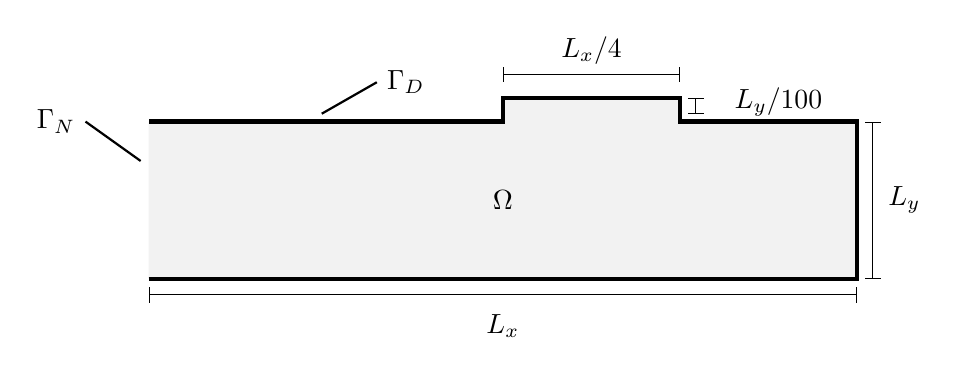
\begin{tikzpicture}
    \fill[black!5!white] (0, 0) to (9, 0) to (9, 2) to (6.75, 2) to (6.75, 2.3) to (4.5, 2.3) to (4.5, 2) to (0, 2);
    \draw[ultra thick] (0, 0) to (9, 0) to (9, 2) to (6.75, 2) to (6.75, 2.3) to (4.5, 2.3) to (4.5, 2) to (0, 2);
    \draw[thick] (-0.8, 2) node[left] {$\Gamma_N$} to (-0.1, 1.5);
    \draw[thick] (2.9, 2.5) node[right] {$\Gamma_D$} to (2.2, 2.1);
    \draw[|-|] (0, -0.2) to (9, -0.2);
    \draw[|-|] (9.2, 0) to (9.2, 2);
    \draw[|-|] (6.75, 2.6) to (4.5, 2.6);
    \draw[|-|] (6.95, 2.1) to (6.95, 2.3);
    \node at (4.5, -0.6) {$L_x$};
    \node at (9.6, 1) {$L_y$};
    \node at (5.626, 2.9) {$L_x / 4$};
    \node at (8, 2.25) {$L_y / 100$};
    \node at (4.5, 1) {$\Omega$};
\end{tikzpicture}

    \caption{A tiny cubby is introduced alongside one of the edges in order to
    break the linear dependence of solutions restricted to a trace. It extends
    along a quarter of the length of the cavity but extends outwards only by
    1/100-th (sketch not drawn to scale!) of the height of the cavity.}
    \label{fig:rectangular-cavity-cubby}
\end{figure}

Despite only adding a minor perturbation to the geometry of the cavity, the improved
convergence behavior may immediately be seen in Figure \ref{fig:rectangular-cubby-trace-errornorm}.

\begin{figure}[ht]
    \centering
    %% Creator: Matplotlib, PGF backend
%%
%% To include the figure in your LaTeX document, write
%%   \input{<filename>.pgf}
%%
%% Make sure the required packages are loaded in your preamble
%%   \usepackage{pgf}
%%
%% Also ensure that all the required font packages are loaded; for instance,
%% the lmodern package is sometimes necessary when using math font.
%%   \usepackage{lmodern}
%%
%% Figures using additional raster images can only be included by \input if
%% they are in the same directory as the main LaTeX file. For loading figures
%% from other directories you can use the `import` package
%%   \usepackage{import}
%%
%% and then include the figures with
%%   \import{<path to file>}{<filename>.pgf}
%%
%% Matplotlib used the following preamble
%%   \usepackage{fontspec}
%%   \setmainfont{DejaVuSans.ttf}[Path=\detokenize{C:/Users/Fabio/Anaconda3/Lib/site-packages/matplotlib/mpl-data/fonts/ttf/}]
%%   \setsansfont{DejaVuSans.ttf}[Path=\detokenize{C:/Users/Fabio/Anaconda3/Lib/site-packages/matplotlib/mpl-data/fonts/ttf/}]
%%   \setmonofont{DejaVuSansMono.ttf}[Path=\detokenize{C:/Users/Fabio/Anaconda3/Lib/site-packages/matplotlib/mpl-data/fonts/ttf/}]
%%
\begingroup%
\makeatletter%
\begin{pgfpicture}%
\pgfpathrectangle{\pgfpointorigin}{\pgfqpoint{5.314460in}{3.950463in}}%
\pgfusepath{use as bounding box, clip}%
\begin{pgfscope}%
\pgfsetbuttcap%
\pgfsetmiterjoin%
\pgfsetlinewidth{0.000000pt}%
\definecolor{currentstroke}{rgb}{1.000000,1.000000,1.000000}%
\pgfsetstrokecolor{currentstroke}%
\pgfsetstrokeopacity{0.000000}%
\pgfsetdash{}{0pt}%
\pgfpathmoveto{\pgfqpoint{0.000000in}{0.000000in}}%
\pgfpathlineto{\pgfqpoint{5.314460in}{0.000000in}}%
\pgfpathlineto{\pgfqpoint{5.314460in}{3.950463in}}%
\pgfpathlineto{\pgfqpoint{0.000000in}{3.950463in}}%
\pgfpathlineto{\pgfqpoint{0.000000in}{0.000000in}}%
\pgfpathclose%
\pgfusepath{}%
\end{pgfscope}%
\begin{pgfscope}%
\pgfsetbuttcap%
\pgfsetmiterjoin%
\definecolor{currentfill}{rgb}{1.000000,1.000000,1.000000}%
\pgfsetfillcolor{currentfill}%
\pgfsetlinewidth{0.000000pt}%
\definecolor{currentstroke}{rgb}{0.000000,0.000000,0.000000}%
\pgfsetstrokecolor{currentstroke}%
\pgfsetstrokeopacity{0.000000}%
\pgfsetdash{}{0pt}%
\pgfpathmoveto{\pgfqpoint{0.816045in}{0.823031in}}%
\pgfpathlineto{\pgfqpoint{5.117295in}{0.823031in}}%
\pgfpathlineto{\pgfqpoint{5.117295in}{3.568486in}}%
\pgfpathlineto{\pgfqpoint{0.816045in}{3.568486in}}%
\pgfpathlineto{\pgfqpoint{0.816045in}{0.823031in}}%
\pgfpathclose%
\pgfusepath{fill}%
\end{pgfscope}%
\begin{pgfscope}%
\pgfsetbuttcap%
\pgfsetroundjoin%
\definecolor{currentfill}{rgb}{0.000000,0.000000,0.000000}%
\pgfsetfillcolor{currentfill}%
\pgfsetlinewidth{0.803000pt}%
\definecolor{currentstroke}{rgb}{0.000000,0.000000,0.000000}%
\pgfsetstrokecolor{currentstroke}%
\pgfsetdash{}{0pt}%
\pgfsys@defobject{currentmarker}{\pgfqpoint{0.000000in}{-0.048611in}}{\pgfqpoint{0.000000in}{0.000000in}}{%
\pgfpathmoveto{\pgfqpoint{0.000000in}{0.000000in}}%
\pgfpathlineto{\pgfqpoint{0.000000in}{-0.048611in}}%
\pgfusepath{stroke,fill}%
}%
\begin{pgfscope}%
\pgfsys@transformshift{0.816045in}{0.823031in}%
\pgfsys@useobject{currentmarker}{}%
\end{pgfscope}%
\end{pgfscope}%
\begin{pgfscope}%
\pgfsetbuttcap%
\pgfsetroundjoin%
\definecolor{currentfill}{rgb}{0.000000,0.000000,0.000000}%
\pgfsetfillcolor{currentfill}%
\pgfsetlinewidth{0.803000pt}%
\definecolor{currentstroke}{rgb}{0.000000,0.000000,0.000000}%
\pgfsetstrokecolor{currentstroke}%
\pgfsetdash{}{0pt}%
\pgfsys@defobject{currentmarker}{\pgfqpoint{0.000000in}{-0.048611in}}{\pgfqpoint{0.000000in}{0.000000in}}{%
\pgfpathmoveto{\pgfqpoint{0.000000in}{0.000000in}}%
\pgfpathlineto{\pgfqpoint{0.000000in}{-0.048611in}}%
\pgfusepath{stroke,fill}%
}%
\begin{pgfscope}%
\pgfsys@transformshift{1.676295in}{0.823031in}%
\pgfsys@useobject{currentmarker}{}%
\end{pgfscope}%
\end{pgfscope}%
\begin{pgfscope}%
\pgfsetbuttcap%
\pgfsetroundjoin%
\definecolor{currentfill}{rgb}{0.000000,0.000000,0.000000}%
\pgfsetfillcolor{currentfill}%
\pgfsetlinewidth{0.803000pt}%
\definecolor{currentstroke}{rgb}{0.000000,0.000000,0.000000}%
\pgfsetstrokecolor{currentstroke}%
\pgfsetdash{}{0pt}%
\pgfsys@defobject{currentmarker}{\pgfqpoint{0.000000in}{-0.048611in}}{\pgfqpoint{0.000000in}{0.000000in}}{%
\pgfpathmoveto{\pgfqpoint{0.000000in}{0.000000in}}%
\pgfpathlineto{\pgfqpoint{0.000000in}{-0.048611in}}%
\pgfusepath{stroke,fill}%
}%
\begin{pgfscope}%
\pgfsys@transformshift{2.536545in}{0.823031in}%
\pgfsys@useobject{currentmarker}{}%
\end{pgfscope}%
\end{pgfscope}%
\begin{pgfscope}%
\pgfsetbuttcap%
\pgfsetroundjoin%
\definecolor{currentfill}{rgb}{0.000000,0.000000,0.000000}%
\pgfsetfillcolor{currentfill}%
\pgfsetlinewidth{0.803000pt}%
\definecolor{currentstroke}{rgb}{0.000000,0.000000,0.000000}%
\pgfsetstrokecolor{currentstroke}%
\pgfsetdash{}{0pt}%
\pgfsys@defobject{currentmarker}{\pgfqpoint{0.000000in}{-0.048611in}}{\pgfqpoint{0.000000in}{0.000000in}}{%
\pgfpathmoveto{\pgfqpoint{0.000000in}{0.000000in}}%
\pgfpathlineto{\pgfqpoint{0.000000in}{-0.048611in}}%
\pgfusepath{stroke,fill}%
}%
\begin{pgfscope}%
\pgfsys@transformshift{3.396795in}{0.823031in}%
\pgfsys@useobject{currentmarker}{}%
\end{pgfscope}%
\end{pgfscope}%
\begin{pgfscope}%
\pgfsetbuttcap%
\pgfsetroundjoin%
\definecolor{currentfill}{rgb}{0.000000,0.000000,0.000000}%
\pgfsetfillcolor{currentfill}%
\pgfsetlinewidth{0.803000pt}%
\definecolor{currentstroke}{rgb}{0.000000,0.000000,0.000000}%
\pgfsetstrokecolor{currentstroke}%
\pgfsetdash{}{0pt}%
\pgfsys@defobject{currentmarker}{\pgfqpoint{0.000000in}{-0.048611in}}{\pgfqpoint{0.000000in}{0.000000in}}{%
\pgfpathmoveto{\pgfqpoint{0.000000in}{0.000000in}}%
\pgfpathlineto{\pgfqpoint{0.000000in}{-0.048611in}}%
\pgfusepath{stroke,fill}%
}%
\begin{pgfscope}%
\pgfsys@transformshift{4.257045in}{0.823031in}%
\pgfsys@useobject{currentmarker}{}%
\end{pgfscope}%
\end{pgfscope}%
\begin{pgfscope}%
\pgfsetbuttcap%
\pgfsetroundjoin%
\definecolor{currentfill}{rgb}{0.000000,0.000000,0.000000}%
\pgfsetfillcolor{currentfill}%
\pgfsetlinewidth{0.803000pt}%
\definecolor{currentstroke}{rgb}{0.000000,0.000000,0.000000}%
\pgfsetstrokecolor{currentstroke}%
\pgfsetdash{}{0pt}%
\pgfsys@defobject{currentmarker}{\pgfqpoint{0.000000in}{-0.048611in}}{\pgfqpoint{0.000000in}{0.000000in}}{%
\pgfpathmoveto{\pgfqpoint{0.000000in}{0.000000in}}%
\pgfpathlineto{\pgfqpoint{0.000000in}{-0.048611in}}%
\pgfusepath{stroke,fill}%
}%
\begin{pgfscope}%
\pgfsys@transformshift{5.117295in}{0.823031in}%
\pgfsys@useobject{currentmarker}{}%
\end{pgfscope}%
\end{pgfscope}%
\begin{pgfscope}%
\pgfpathrectangle{\pgfqpoint{0.816045in}{0.823031in}}{\pgfqpoint{4.301250in}{2.745455in}}%
\pgfusepath{clip}%
\pgfsetrectcap%
\pgfsetroundjoin%
\pgfsetlinewidth{0.803000pt}%
\definecolor{currentstroke}{rgb}{0.690196,0.690196,0.690196}%
\pgfsetstrokecolor{currentstroke}%
\pgfsetdash{}{0pt}%
\pgfpathmoveto{\pgfqpoint{0.816045in}{1.124514in}}%
\pgfpathlineto{\pgfqpoint{5.117295in}{1.124514in}}%
\pgfusepath{stroke}%
\end{pgfscope}%
\begin{pgfscope}%
\pgfsetbuttcap%
\pgfsetroundjoin%
\definecolor{currentfill}{rgb}{0.000000,0.000000,0.000000}%
\pgfsetfillcolor{currentfill}%
\pgfsetlinewidth{0.803000pt}%
\definecolor{currentstroke}{rgb}{0.000000,0.000000,0.000000}%
\pgfsetstrokecolor{currentstroke}%
\pgfsetdash{}{0pt}%
\pgfsys@defobject{currentmarker}{\pgfqpoint{-0.048611in}{0.000000in}}{\pgfqpoint{-0.000000in}{0.000000in}}{%
\pgfpathmoveto{\pgfqpoint{-0.000000in}{0.000000in}}%
\pgfpathlineto{\pgfqpoint{-0.048611in}{0.000000in}}%
\pgfusepath{stroke,fill}%
}%
\begin{pgfscope}%
\pgfsys@transformshift{0.816045in}{1.124514in}%
\pgfsys@useobject{currentmarker}{}%
\end{pgfscope}%
\end{pgfscope}%
\begin{pgfscope}%
\definecolor{textcolor}{rgb}{0.000000,0.000000,0.000000}%
\pgfsetstrokecolor{textcolor}%
\pgfsetfillcolor{textcolor}%
\pgftext[x=0.408944in, y=1.066477in, left, base]{\color{textcolor}\rmfamily\fontsize{11.000000}{13.200000}\selectfont \(\displaystyle {10^{-8}}\)}%
\end{pgfscope}%
\begin{pgfscope}%
\pgfpathrectangle{\pgfqpoint{0.816045in}{0.823031in}}{\pgfqpoint{4.301250in}{2.745455in}}%
\pgfusepath{clip}%
\pgfsetrectcap%
\pgfsetroundjoin%
\pgfsetlinewidth{0.803000pt}%
\definecolor{currentstroke}{rgb}{0.690196,0.690196,0.690196}%
\pgfsetstrokecolor{currentstroke}%
\pgfsetdash{}{0pt}%
\pgfpathmoveto{\pgfqpoint{0.816045in}{1.546434in}}%
\pgfpathlineto{\pgfqpoint{5.117295in}{1.546434in}}%
\pgfusepath{stroke}%
\end{pgfscope}%
\begin{pgfscope}%
\pgfsetbuttcap%
\pgfsetroundjoin%
\definecolor{currentfill}{rgb}{0.000000,0.000000,0.000000}%
\pgfsetfillcolor{currentfill}%
\pgfsetlinewidth{0.803000pt}%
\definecolor{currentstroke}{rgb}{0.000000,0.000000,0.000000}%
\pgfsetstrokecolor{currentstroke}%
\pgfsetdash{}{0pt}%
\pgfsys@defobject{currentmarker}{\pgfqpoint{-0.048611in}{0.000000in}}{\pgfqpoint{-0.000000in}{0.000000in}}{%
\pgfpathmoveto{\pgfqpoint{-0.000000in}{0.000000in}}%
\pgfpathlineto{\pgfqpoint{-0.048611in}{0.000000in}}%
\pgfusepath{stroke,fill}%
}%
\begin{pgfscope}%
\pgfsys@transformshift{0.816045in}{1.546434in}%
\pgfsys@useobject{currentmarker}{}%
\end{pgfscope}%
\end{pgfscope}%
\begin{pgfscope}%
\definecolor{textcolor}{rgb}{0.000000,0.000000,0.000000}%
\pgfsetstrokecolor{textcolor}%
\pgfsetfillcolor{textcolor}%
\pgftext[x=0.408944in, y=1.488396in, left, base]{\color{textcolor}\rmfamily\fontsize{11.000000}{13.200000}\selectfont \(\displaystyle {10^{-6}}\)}%
\end{pgfscope}%
\begin{pgfscope}%
\pgfpathrectangle{\pgfqpoint{0.816045in}{0.823031in}}{\pgfqpoint{4.301250in}{2.745455in}}%
\pgfusepath{clip}%
\pgfsetrectcap%
\pgfsetroundjoin%
\pgfsetlinewidth{0.803000pt}%
\definecolor{currentstroke}{rgb}{0.690196,0.690196,0.690196}%
\pgfsetstrokecolor{currentstroke}%
\pgfsetdash{}{0pt}%
\pgfpathmoveto{\pgfqpoint{0.816045in}{1.968353in}}%
\pgfpathlineto{\pgfqpoint{5.117295in}{1.968353in}}%
\pgfusepath{stroke}%
\end{pgfscope}%
\begin{pgfscope}%
\pgfsetbuttcap%
\pgfsetroundjoin%
\definecolor{currentfill}{rgb}{0.000000,0.000000,0.000000}%
\pgfsetfillcolor{currentfill}%
\pgfsetlinewidth{0.803000pt}%
\definecolor{currentstroke}{rgb}{0.000000,0.000000,0.000000}%
\pgfsetstrokecolor{currentstroke}%
\pgfsetdash{}{0pt}%
\pgfsys@defobject{currentmarker}{\pgfqpoint{-0.048611in}{0.000000in}}{\pgfqpoint{-0.000000in}{0.000000in}}{%
\pgfpathmoveto{\pgfqpoint{-0.000000in}{0.000000in}}%
\pgfpathlineto{\pgfqpoint{-0.048611in}{0.000000in}}%
\pgfusepath{stroke,fill}%
}%
\begin{pgfscope}%
\pgfsys@transformshift{0.816045in}{1.968353in}%
\pgfsys@useobject{currentmarker}{}%
\end{pgfscope}%
\end{pgfscope}%
\begin{pgfscope}%
\definecolor{textcolor}{rgb}{0.000000,0.000000,0.000000}%
\pgfsetstrokecolor{textcolor}%
\pgfsetfillcolor{textcolor}%
\pgftext[x=0.408944in, y=1.910316in, left, base]{\color{textcolor}\rmfamily\fontsize{11.000000}{13.200000}\selectfont \(\displaystyle {10^{-4}}\)}%
\end{pgfscope}%
\begin{pgfscope}%
\pgfpathrectangle{\pgfqpoint{0.816045in}{0.823031in}}{\pgfqpoint{4.301250in}{2.745455in}}%
\pgfusepath{clip}%
\pgfsetrectcap%
\pgfsetroundjoin%
\pgfsetlinewidth{0.803000pt}%
\definecolor{currentstroke}{rgb}{0.690196,0.690196,0.690196}%
\pgfsetstrokecolor{currentstroke}%
\pgfsetdash{}{0pt}%
\pgfpathmoveto{\pgfqpoint{0.816045in}{2.390273in}}%
\pgfpathlineto{\pgfqpoint{5.117295in}{2.390273in}}%
\pgfusepath{stroke}%
\end{pgfscope}%
\begin{pgfscope}%
\pgfsetbuttcap%
\pgfsetroundjoin%
\definecolor{currentfill}{rgb}{0.000000,0.000000,0.000000}%
\pgfsetfillcolor{currentfill}%
\pgfsetlinewidth{0.803000pt}%
\definecolor{currentstroke}{rgb}{0.000000,0.000000,0.000000}%
\pgfsetstrokecolor{currentstroke}%
\pgfsetdash{}{0pt}%
\pgfsys@defobject{currentmarker}{\pgfqpoint{-0.048611in}{0.000000in}}{\pgfqpoint{-0.000000in}{0.000000in}}{%
\pgfpathmoveto{\pgfqpoint{-0.000000in}{0.000000in}}%
\pgfpathlineto{\pgfqpoint{-0.048611in}{0.000000in}}%
\pgfusepath{stroke,fill}%
}%
\begin{pgfscope}%
\pgfsys@transformshift{0.816045in}{2.390273in}%
\pgfsys@useobject{currentmarker}{}%
\end{pgfscope}%
\end{pgfscope}%
\begin{pgfscope}%
\definecolor{textcolor}{rgb}{0.000000,0.000000,0.000000}%
\pgfsetstrokecolor{textcolor}%
\pgfsetfillcolor{textcolor}%
\pgftext[x=0.408944in, y=2.332235in, left, base]{\color{textcolor}\rmfamily\fontsize{11.000000}{13.200000}\selectfont \(\displaystyle {10^{-2}}\)}%
\end{pgfscope}%
\begin{pgfscope}%
\pgfpathrectangle{\pgfqpoint{0.816045in}{0.823031in}}{\pgfqpoint{4.301250in}{2.745455in}}%
\pgfusepath{clip}%
\pgfsetrectcap%
\pgfsetroundjoin%
\pgfsetlinewidth{0.803000pt}%
\definecolor{currentstroke}{rgb}{0.690196,0.690196,0.690196}%
\pgfsetstrokecolor{currentstroke}%
\pgfsetdash{}{0pt}%
\pgfpathmoveto{\pgfqpoint{0.816045in}{2.812192in}}%
\pgfpathlineto{\pgfqpoint{5.117295in}{2.812192in}}%
\pgfusepath{stroke}%
\end{pgfscope}%
\begin{pgfscope}%
\pgfsetbuttcap%
\pgfsetroundjoin%
\definecolor{currentfill}{rgb}{0.000000,0.000000,0.000000}%
\pgfsetfillcolor{currentfill}%
\pgfsetlinewidth{0.803000pt}%
\definecolor{currentstroke}{rgb}{0.000000,0.000000,0.000000}%
\pgfsetstrokecolor{currentstroke}%
\pgfsetdash{}{0pt}%
\pgfsys@defobject{currentmarker}{\pgfqpoint{-0.048611in}{0.000000in}}{\pgfqpoint{-0.000000in}{0.000000in}}{%
\pgfpathmoveto{\pgfqpoint{-0.000000in}{0.000000in}}%
\pgfpathlineto{\pgfqpoint{-0.048611in}{0.000000in}}%
\pgfusepath{stroke,fill}%
}%
\begin{pgfscope}%
\pgfsys@transformshift{0.816045in}{2.812192in}%
\pgfsys@useobject{currentmarker}{}%
\end{pgfscope}%
\end{pgfscope}%
\begin{pgfscope}%
\definecolor{textcolor}{rgb}{0.000000,0.000000,0.000000}%
\pgfsetstrokecolor{textcolor}%
\pgfsetfillcolor{textcolor}%
\pgftext[x=0.500767in, y=2.754155in, left, base]{\color{textcolor}\rmfamily\fontsize{11.000000}{13.200000}\selectfont \(\displaystyle {10^{0}}\)}%
\end{pgfscope}%
\begin{pgfscope}%
\pgfpathrectangle{\pgfqpoint{0.816045in}{0.823031in}}{\pgfqpoint{4.301250in}{2.745455in}}%
\pgfusepath{clip}%
\pgfsetrectcap%
\pgfsetroundjoin%
\pgfsetlinewidth{0.803000pt}%
\definecolor{currentstroke}{rgb}{0.690196,0.690196,0.690196}%
\pgfsetstrokecolor{currentstroke}%
\pgfsetdash{}{0pt}%
\pgfpathmoveto{\pgfqpoint{0.816045in}{3.234112in}}%
\pgfpathlineto{\pgfqpoint{5.117295in}{3.234112in}}%
\pgfusepath{stroke}%
\end{pgfscope}%
\begin{pgfscope}%
\pgfsetbuttcap%
\pgfsetroundjoin%
\definecolor{currentfill}{rgb}{0.000000,0.000000,0.000000}%
\pgfsetfillcolor{currentfill}%
\pgfsetlinewidth{0.803000pt}%
\definecolor{currentstroke}{rgb}{0.000000,0.000000,0.000000}%
\pgfsetstrokecolor{currentstroke}%
\pgfsetdash{}{0pt}%
\pgfsys@defobject{currentmarker}{\pgfqpoint{-0.048611in}{0.000000in}}{\pgfqpoint{-0.000000in}{0.000000in}}{%
\pgfpathmoveto{\pgfqpoint{-0.000000in}{0.000000in}}%
\pgfpathlineto{\pgfqpoint{-0.048611in}{0.000000in}}%
\pgfusepath{stroke,fill}%
}%
\begin{pgfscope}%
\pgfsys@transformshift{0.816045in}{3.234112in}%
\pgfsys@useobject{currentmarker}{}%
\end{pgfscope}%
\end{pgfscope}%
\begin{pgfscope}%
\definecolor{textcolor}{rgb}{0.000000,0.000000,0.000000}%
\pgfsetstrokecolor{textcolor}%
\pgfsetfillcolor{textcolor}%
\pgftext[x=0.500767in, y=3.176074in, left, base]{\color{textcolor}\rmfamily\fontsize{11.000000}{13.200000}\selectfont \(\displaystyle {10^{2}}\)}%
\end{pgfscope}%
\begin{pgfscope}%
\definecolor{textcolor}{rgb}{0.000000,0.000000,0.000000}%
\pgfsetstrokecolor{textcolor}%
\pgfsetfillcolor{textcolor}%
\pgftext[x=0.353389in,y=2.195759in,,bottom,rotate=90.000000]{\color{textcolor}\rmfamily\fontsize{11.000000}{13.200000}\selectfont \(\displaystyle ||\mathbf{\tilde{u}}_z^{(S)}|_{\Gamma_N}(\omega) - \mathbf{u}|_{\Gamma_N}(\omega)||_{M(\Gamma_N)} / ||\mathbf{\tilde{u}}_z^{(S)}|_{\Gamma_N}(\omega)||_{M(\Gamma_N)}\)}%
\end{pgfscope}%
\begin{pgfscope}%
\pgfpathrectangle{\pgfqpoint{0.816045in}{0.823031in}}{\pgfqpoint{4.301250in}{2.745455in}}%
\pgfusepath{clip}%
\pgfsetrectcap%
\pgfsetroundjoin%
\pgfsetlinewidth{1.505625pt}%
\definecolor{currentstroke}{rgb}{0.001462,0.000466,0.013866}%
\pgfsetstrokecolor{currentstroke}%
\pgfsetdash{}{0pt}%
\pgfpathmoveto{\pgfqpoint{0.813895in}{2.418879in}}%
\pgfpathlineto{\pgfqpoint{0.818200in}{2.421382in}}%
\pgfpathlineto{\pgfqpoint{0.822506in}{2.524354in}}%
\pgfpathlineto{\pgfqpoint{0.831117in}{2.606920in}}%
\pgfpathlineto{\pgfqpoint{0.839728in}{2.653565in}}%
\pgfpathlineto{\pgfqpoint{0.852645in}{2.701917in}}%
\pgfpathlineto{\pgfqpoint{0.869867in}{2.749927in}}%
\pgfpathlineto{\pgfqpoint{0.891395in}{2.799565in}}%
\pgfpathlineto{\pgfqpoint{0.934450in}{2.896812in}}%
\pgfpathlineto{\pgfqpoint{0.947367in}{2.932906in}}%
\pgfpathlineto{\pgfqpoint{0.960283in}{2.979168in}}%
\pgfpathlineto{\pgfqpoint{0.968894in}{3.022411in}}%
\pgfpathlineto{\pgfqpoint{0.973200in}{3.052088in}}%
\pgfpathlineto{\pgfqpoint{0.977506in}{3.093215in}}%
\pgfpathlineto{\pgfqpoint{0.981811in}{3.163152in}}%
\pgfpathlineto{\pgfqpoint{0.986117in}{3.299494in}}%
\pgfpathlineto{\pgfqpoint{0.990422in}{3.148337in}}%
\pgfpathlineto{\pgfqpoint{0.994728in}{3.092540in}}%
\pgfpathlineto{\pgfqpoint{1.003339in}{3.035979in}}%
\pgfpathlineto{\pgfqpoint{1.011950in}{3.003797in}}%
\pgfpathlineto{\pgfqpoint{1.020561in}{2.981793in}}%
\pgfpathlineto{\pgfqpoint{1.033478in}{2.958551in}}%
\pgfpathlineto{\pgfqpoint{1.046394in}{2.941917in}}%
\pgfpathlineto{\pgfqpoint{1.063617in}{2.925627in}}%
\pgfpathlineto{\pgfqpoint{1.080839in}{2.913472in}}%
\pgfpathlineto{\pgfqpoint{1.102367in}{2.901913in}}%
\pgfpathlineto{\pgfqpoint{1.128200in}{2.891459in}}%
\pgfpathlineto{\pgfqpoint{1.162644in}{2.881150in}}%
\pgfpathlineto{\pgfqpoint{1.205700in}{2.871837in}}%
\pgfpathlineto{\pgfqpoint{1.261672in}{2.863244in}}%
\pgfpathlineto{\pgfqpoint{1.334866in}{2.855447in}}%
\pgfpathlineto{\pgfqpoint{1.433894in}{2.848307in}}%
\pgfpathlineto{\pgfqpoint{1.571672in}{2.841751in}}%
\pgfpathlineto{\pgfqpoint{1.774033in}{2.835477in}}%
\pgfpathlineto{\pgfqpoint{2.140004in}{2.827747in}}%
\pgfpathlineto{\pgfqpoint{2.592087in}{2.817538in}}%
\pgfpathlineto{\pgfqpoint{2.794448in}{2.809933in}}%
\pgfpathlineto{\pgfqpoint{2.932226in}{2.801780in}}%
\pgfpathlineto{\pgfqpoint{3.031254in}{2.792955in}}%
\pgfpathlineto{\pgfqpoint{3.104448in}{2.783550in}}%
\pgfpathlineto{\pgfqpoint{3.160420in}{2.773560in}}%
\pgfpathlineto{\pgfqpoint{3.207781in}{2.762001in}}%
\pgfpathlineto{\pgfqpoint{3.242226in}{2.750757in}}%
\pgfpathlineto{\pgfqpoint{3.272364in}{2.737845in}}%
\pgfpathlineto{\pgfqpoint{3.298198in}{2.723222in}}%
\pgfpathlineto{\pgfqpoint{3.319725in}{2.707066in}}%
\pgfpathlineto{\pgfqpoint{3.336948in}{2.689985in}}%
\pgfpathlineto{\pgfqpoint{3.349864in}{2.673321in}}%
\pgfpathlineto{\pgfqpoint{3.362781in}{2.651271in}}%
\pgfpathlineto{\pgfqpoint{3.371392in}{2.631679in}}%
\pgfpathlineto{\pgfqpoint{3.380003in}{2.605275in}}%
\pgfpathlineto{\pgfqpoint{3.388614in}{2.565653in}}%
\pgfpathlineto{\pgfqpoint{3.392920in}{2.535427in}}%
\pgfpathlineto{\pgfqpoint{3.397225in}{2.488467in}}%
\pgfpathlineto{\pgfqpoint{3.401531in}{2.381986in}}%
\pgfpathlineto{\pgfqpoint{3.405837in}{2.402844in}}%
\pgfpathlineto{\pgfqpoint{3.410142in}{2.498632in}}%
\pgfpathlineto{\pgfqpoint{3.418753in}{2.576942in}}%
\pgfpathlineto{\pgfqpoint{3.427364in}{2.620412in}}%
\pgfpathlineto{\pgfqpoint{3.440281in}{2.663952in}}%
\pgfpathlineto{\pgfqpoint{3.453198in}{2.695626in}}%
\pgfpathlineto{\pgfqpoint{3.470420in}{2.728642in}}%
\pgfpathlineto{\pgfqpoint{3.491948in}{2.761896in}}%
\pgfpathlineto{\pgfqpoint{3.517781in}{2.795468in}}%
\pgfpathlineto{\pgfqpoint{3.552225in}{2.834857in}}%
\pgfpathlineto{\pgfqpoint{3.646947in}{2.940360in}}%
\pgfpathlineto{\pgfqpoint{3.672781in}{2.975413in}}%
\pgfpathlineto{\pgfqpoint{3.690003in}{3.003141in}}%
\pgfpathlineto{\pgfqpoint{3.707225in}{3.037173in}}%
\pgfpathlineto{\pgfqpoint{3.720142in}{3.070157in}}%
\pgfpathlineto{\pgfqpoint{3.728753in}{3.098712in}}%
\pgfpathlineto{\pgfqpoint{3.737364in}{3.137429in}}%
\pgfpathlineto{\pgfqpoint{3.741670in}{3.163989in}}%
\pgfpathlineto{\pgfqpoint{3.745975in}{3.200232in}}%
\pgfpathlineto{\pgfqpoint{3.750281in}{3.258665in}}%
\pgfpathlineto{\pgfqpoint{3.754586in}{3.443692in}}%
\pgfpathlineto{\pgfqpoint{3.758892in}{3.289989in}}%
\pgfpathlineto{\pgfqpoint{3.763197in}{3.219687in}}%
\pgfpathlineto{\pgfqpoint{3.771808in}{3.154914in}}%
\pgfpathlineto{\pgfqpoint{3.780419in}{3.119011in}}%
\pgfpathlineto{\pgfqpoint{3.789031in}{3.094477in}}%
\pgfpathlineto{\pgfqpoint{3.801947in}{3.068380in}}%
\pgfpathlineto{\pgfqpoint{3.814864in}{3.049496in}}%
\pgfpathlineto{\pgfqpoint{3.832086in}{3.030784in}}%
\pgfpathlineto{\pgfqpoint{3.849308in}{3.016678in}}%
\pgfpathlineto{\pgfqpoint{3.870836in}{3.003176in}}%
\pgfpathlineto{\pgfqpoint{3.896669in}{2.990967in}}%
\pgfpathlineto{\pgfqpoint{3.926808in}{2.980372in}}%
\pgfpathlineto{\pgfqpoint{3.961253in}{2.971512in}}%
\pgfpathlineto{\pgfqpoint{4.004308in}{2.963776in}}%
\pgfpathlineto{\pgfqpoint{4.055975in}{2.957925in}}%
\pgfpathlineto{\pgfqpoint{4.111947in}{2.954695in}}%
\pgfpathlineto{\pgfqpoint{4.176530in}{2.954211in}}%
\pgfpathlineto{\pgfqpoint{4.241113in}{2.956950in}}%
\pgfpathlineto{\pgfqpoint{4.301391in}{2.962684in}}%
\pgfpathlineto{\pgfqpoint{4.353058in}{2.970661in}}%
\pgfpathlineto{\pgfqpoint{4.396113in}{2.980261in}}%
\pgfpathlineto{\pgfqpoint{4.430558in}{2.990681in}}%
\pgfpathlineto{\pgfqpoint{4.460697in}{3.002682in}}%
\pgfpathlineto{\pgfqpoint{4.486530in}{3.016104in}}%
\pgfpathlineto{\pgfqpoint{4.508058in}{3.030579in}}%
\pgfpathlineto{\pgfqpoint{4.525280in}{3.045383in}}%
\pgfpathlineto{\pgfqpoint{4.542502in}{3.064603in}}%
\pgfpathlineto{\pgfqpoint{4.555419in}{3.083583in}}%
\pgfpathlineto{\pgfqpoint{4.568335in}{3.109182in}}%
\pgfpathlineto{\pgfqpoint{4.576946in}{3.132583in}}%
\pgfpathlineto{\pgfqpoint{4.585558in}{3.165563in}}%
\pgfpathlineto{\pgfqpoint{4.589863in}{3.188656in}}%
\pgfpathlineto{\pgfqpoint{4.594169in}{3.220259in}}%
\pgfpathlineto{\pgfqpoint{4.598474in}{3.269755in}}%
\pgfpathlineto{\pgfqpoint{4.602780in}{3.377288in}}%
\pgfpathlineto{\pgfqpoint{4.607085in}{3.325373in}}%
\pgfpathlineto{\pgfqpoint{4.611391in}{3.246223in}}%
\pgfpathlineto{\pgfqpoint{4.620002in}{3.173214in}}%
\pgfpathlineto{\pgfqpoint{4.628613in}{3.131667in}}%
\pgfpathlineto{\pgfqpoint{4.641530in}{3.090000in}}%
\pgfpathlineto{\pgfqpoint{4.654446in}{3.059911in}}%
\pgfpathlineto{\pgfqpoint{4.671669in}{3.028970in}}%
\pgfpathlineto{\pgfqpoint{4.688891in}{3.004072in}}%
\pgfpathlineto{\pgfqpoint{4.710419in}{2.978042in}}%
\pgfpathlineto{\pgfqpoint{4.736252in}{2.951445in}}%
\pgfpathlineto{\pgfqpoint{4.770696in}{2.920718in}}%
\pgfpathlineto{\pgfqpoint{4.818057in}{2.883282in}}%
\pgfpathlineto{\pgfqpoint{4.964446in}{2.771219in}}%
\pgfpathlineto{\pgfqpoint{4.994585in}{2.743249in}}%
\pgfpathlineto{\pgfqpoint{5.020418in}{2.715321in}}%
\pgfpathlineto{\pgfqpoint{5.041946in}{2.687355in}}%
\pgfpathlineto{\pgfqpoint{5.059168in}{2.659795in}}%
\pgfpathlineto{\pgfqpoint{5.072085in}{2.634023in}}%
\pgfpathlineto{\pgfqpoint{5.085001in}{2.600523in}}%
\pgfpathlineto{\pgfqpoint{5.093613in}{2.570365in}}%
\pgfpathlineto{\pgfqpoint{5.102224in}{2.527245in}}%
\pgfpathlineto{\pgfqpoint{5.106529in}{2.495577in}}%
\pgfpathlineto{\pgfqpoint{5.110835in}{2.447949in}}%
\pgfpathlineto{\pgfqpoint{5.115140in}{2.346524in}}%
\pgfpathlineto{\pgfqpoint{5.119446in}{2.345516in}}%
\pgfpathlineto{\pgfqpoint{5.119446in}{2.345516in}}%
\pgfusepath{stroke}%
\end{pgfscope}%
\begin{pgfscope}%
\pgfpathrectangle{\pgfqpoint{0.816045in}{0.823031in}}{\pgfqpoint{4.301250in}{2.745455in}}%
\pgfusepath{clip}%
\pgfsetrectcap%
\pgfsetroundjoin%
\pgfsetlinewidth{1.505625pt}%
\definecolor{currentstroke}{rgb}{0.155850,0.044559,0.325338}%
\pgfsetstrokecolor{currentstroke}%
\pgfsetdash{}{0pt}%
\pgfpathmoveto{\pgfqpoint{0.813895in}{2.420633in}}%
\pgfpathlineto{\pgfqpoint{0.818200in}{2.423139in}}%
\pgfpathlineto{\pgfqpoint{0.822506in}{2.526114in}}%
\pgfpathlineto{\pgfqpoint{0.831117in}{2.608685in}}%
\pgfpathlineto{\pgfqpoint{0.839728in}{2.655336in}}%
\pgfpathlineto{\pgfqpoint{0.852645in}{2.703696in}}%
\pgfpathlineto{\pgfqpoint{0.869867in}{2.751716in}}%
\pgfpathlineto{\pgfqpoint{0.891395in}{2.801366in}}%
\pgfpathlineto{\pgfqpoint{0.934450in}{2.898636in}}%
\pgfpathlineto{\pgfqpoint{0.947367in}{2.934737in}}%
\pgfpathlineto{\pgfqpoint{0.960283in}{2.981005in}}%
\pgfpathlineto{\pgfqpoint{0.968894in}{3.024253in}}%
\pgfpathlineto{\pgfqpoint{0.973200in}{3.053932in}}%
\pgfpathlineto{\pgfqpoint{0.977506in}{3.095061in}}%
\pgfpathlineto{\pgfqpoint{0.981811in}{3.165000in}}%
\pgfpathlineto{\pgfqpoint{0.986117in}{3.301344in}}%
\pgfpathlineto{\pgfqpoint{0.990422in}{3.150189in}}%
\pgfpathlineto{\pgfqpoint{0.994728in}{3.094395in}}%
\pgfpathlineto{\pgfqpoint{1.003339in}{3.037837in}}%
\pgfpathlineto{\pgfqpoint{1.011950in}{3.005659in}}%
\pgfpathlineto{\pgfqpoint{1.020561in}{2.983658in}}%
\pgfpathlineto{\pgfqpoint{1.033478in}{2.960422in}}%
\pgfpathlineto{\pgfqpoint{1.046394in}{2.943794in}}%
\pgfpathlineto{\pgfqpoint{1.063617in}{2.927510in}}%
\pgfpathlineto{\pgfqpoint{1.080839in}{2.915362in}}%
\pgfpathlineto{\pgfqpoint{1.102367in}{2.903810in}}%
\pgfpathlineto{\pgfqpoint{1.128200in}{2.893364in}}%
\pgfpathlineto{\pgfqpoint{1.162644in}{2.883065in}}%
\pgfpathlineto{\pgfqpoint{1.205700in}{2.873761in}}%
\pgfpathlineto{\pgfqpoint{1.261672in}{2.865177in}}%
\pgfpathlineto{\pgfqpoint{1.334866in}{2.857385in}}%
\pgfpathlineto{\pgfqpoint{1.433894in}{2.850238in}}%
\pgfpathlineto{\pgfqpoint{1.571672in}{2.843641in}}%
\pgfpathlineto{\pgfqpoint{1.778338in}{2.837121in}}%
\pgfpathlineto{\pgfqpoint{2.191671in}{2.827879in}}%
\pgfpathlineto{\pgfqpoint{2.587782in}{2.817831in}}%
\pgfpathlineto{\pgfqpoint{2.811670in}{2.809211in}}%
\pgfpathlineto{\pgfqpoint{2.979587in}{2.799797in}}%
\pgfpathlineto{\pgfqpoint{3.113059in}{2.789269in}}%
\pgfpathlineto{\pgfqpoint{3.220698in}{2.777699in}}%
\pgfpathlineto{\pgfqpoint{3.306809in}{2.765485in}}%
\pgfpathlineto{\pgfqpoint{3.380003in}{2.752105in}}%
\pgfpathlineto{\pgfqpoint{3.440281in}{2.738147in}}%
\pgfpathlineto{\pgfqpoint{3.491948in}{2.723203in}}%
\pgfpathlineto{\pgfqpoint{3.535003in}{2.707800in}}%
\pgfpathlineto{\pgfqpoint{3.573753in}{2.690693in}}%
\pgfpathlineto{\pgfqpoint{3.603892in}{2.674374in}}%
\pgfpathlineto{\pgfqpoint{3.629725in}{2.657389in}}%
\pgfpathlineto{\pgfqpoint{3.651253in}{2.640226in}}%
\pgfpathlineto{\pgfqpoint{3.672781in}{2.619036in}}%
\pgfpathlineto{\pgfqpoint{3.690003in}{2.597681in}}%
\pgfpathlineto{\pgfqpoint{3.702920in}{2.577668in}}%
\pgfpathlineto{\pgfqpoint{3.715836in}{2.552164in}}%
\pgfpathlineto{\pgfqpoint{3.724447in}{2.530234in}}%
\pgfpathlineto{\pgfqpoint{3.733058in}{2.501518in}}%
\pgfpathlineto{\pgfqpoint{3.741670in}{2.459781in}}%
\pgfpathlineto{\pgfqpoint{3.745975in}{2.428781in}}%
\pgfpathlineto{\pgfqpoint{3.750281in}{2.381801in}}%
\pgfpathlineto{\pgfqpoint{3.754586in}{2.280980in}}%
\pgfpathlineto{\pgfqpoint{3.758892in}{2.280715in}}%
\pgfpathlineto{\pgfqpoint{3.763197in}{2.381185in}}%
\pgfpathlineto{\pgfqpoint{3.771808in}{2.458385in}}%
\pgfpathlineto{\pgfqpoint{3.780419in}{2.499330in}}%
\pgfpathlineto{\pgfqpoint{3.789031in}{2.527245in}}%
\pgfpathlineto{\pgfqpoint{3.801947in}{2.557255in}}%
\pgfpathlineto{\pgfqpoint{3.814864in}{2.579381in}}%
\pgfpathlineto{\pgfqpoint{3.832086in}{2.601821in}}%
\pgfpathlineto{\pgfqpoint{3.849308in}{2.619180in}}%
\pgfpathlineto{\pgfqpoint{3.870836in}{2.636210in}}%
\pgfpathlineto{\pgfqpoint{3.896669in}{2.651954in}}%
\pgfpathlineto{\pgfqpoint{3.922503in}{2.664032in}}%
\pgfpathlineto{\pgfqpoint{3.952642in}{2.674619in}}%
\pgfpathlineto{\pgfqpoint{3.982780in}{2.682139in}}%
\pgfpathlineto{\pgfqpoint{4.017225in}{2.687472in}}%
\pgfpathlineto{\pgfqpoint{4.051669in}{2.689518in}}%
\pgfpathlineto{\pgfqpoint{4.086114in}{2.688152in}}%
\pgfpathlineto{\pgfqpoint{4.116252in}{2.683767in}}%
\pgfpathlineto{\pgfqpoint{4.142086in}{2.677085in}}%
\pgfpathlineto{\pgfqpoint{4.163614in}{2.668849in}}%
\pgfpathlineto{\pgfqpoint{4.185141in}{2.657314in}}%
\pgfpathlineto{\pgfqpoint{4.202363in}{2.644736in}}%
\pgfpathlineto{\pgfqpoint{4.219586in}{2.627686in}}%
\pgfpathlineto{\pgfqpoint{4.232502in}{2.610362in}}%
\pgfpathlineto{\pgfqpoint{4.245419in}{2.586559in}}%
\pgfpathlineto{\pgfqpoint{4.254030in}{2.564570in}}%
\pgfpathlineto{\pgfqpoint{4.262641in}{2.533468in}}%
\pgfpathlineto{\pgfqpoint{4.271252in}{2.482210in}}%
\pgfpathlineto{\pgfqpoint{4.275558in}{2.436714in}}%
\pgfpathlineto{\pgfqpoint{4.279863in}{2.337397in}}%
\pgfpathlineto{\pgfqpoint{4.284169in}{2.338587in}}%
\pgfpathlineto{\pgfqpoint{4.288475in}{2.440583in}}%
\pgfpathlineto{\pgfqpoint{4.297086in}{2.520846in}}%
\pgfpathlineto{\pgfqpoint{4.305697in}{2.564902in}}%
\pgfpathlineto{\pgfqpoint{4.318613in}{2.608802in}}%
\pgfpathlineto{\pgfqpoint{4.331530in}{2.640588in}}%
\pgfpathlineto{\pgfqpoint{4.348752in}{2.673543in}}%
\pgfpathlineto{\pgfqpoint{4.370280in}{2.706495in}}%
\pgfpathlineto{\pgfqpoint{4.396113in}{2.739483in}}%
\pgfpathlineto{\pgfqpoint{4.430558in}{2.777941in}}%
\pgfpathlineto{\pgfqpoint{4.503752in}{2.857682in}}%
\pgfpathlineto{\pgfqpoint{4.525280in}{2.885615in}}%
\pgfpathlineto{\pgfqpoint{4.542502in}{2.912130in}}%
\pgfpathlineto{\pgfqpoint{4.555419in}{2.936248in}}%
\pgfpathlineto{\pgfqpoint{4.568335in}{2.966724in}}%
\pgfpathlineto{\pgfqpoint{4.576946in}{2.993243in}}%
\pgfpathlineto{\pgfqpoint{4.585558in}{3.029239in}}%
\pgfpathlineto{\pgfqpoint{4.594169in}{3.086856in}}%
\pgfpathlineto{\pgfqpoint{4.598474in}{3.137777in}}%
\pgfpathlineto{\pgfqpoint{4.602780in}{3.246713in}}%
\pgfpathlineto{\pgfqpoint{4.607085in}{3.196179in}}%
\pgfpathlineto{\pgfqpoint{4.611391in}{3.118390in}}%
\pgfpathlineto{\pgfqpoint{4.620002in}{3.048039in}}%
\pgfpathlineto{\pgfqpoint{4.628613in}{3.009071in}}%
\pgfpathlineto{\pgfqpoint{4.637224in}{2.982070in}}%
\pgfpathlineto{\pgfqpoint{4.650141in}{2.952609in}}%
\pgfpathlineto{\pgfqpoint{4.663057in}{2.930459in}}%
\pgfpathlineto{\pgfqpoint{4.680280in}{2.907340in}}%
\pgfpathlineto{\pgfqpoint{4.701807in}{2.884489in}}%
\pgfpathlineto{\pgfqpoint{4.727641in}{2.862207in}}%
\pgfpathlineto{\pgfqpoint{4.762085in}{2.837377in}}%
\pgfpathlineto{\pgfqpoint{4.809446in}{2.807758in}}%
\pgfpathlineto{\pgfqpoint{4.938613in}{2.729248in}}%
\pgfpathlineto{\pgfqpoint{4.973057in}{2.704074in}}%
\pgfpathlineto{\pgfqpoint{5.003196in}{2.678167in}}%
\pgfpathlineto{\pgfqpoint{5.024724in}{2.656049in}}%
\pgfpathlineto{\pgfqpoint{5.041946in}{2.634927in}}%
\pgfpathlineto{\pgfqpoint{5.059168in}{2.608973in}}%
\pgfpathlineto{\pgfqpoint{5.072085in}{2.584367in}}%
\pgfpathlineto{\pgfqpoint{5.085001in}{2.552000in}}%
\pgfpathlineto{\pgfqpoint{5.093613in}{2.522580in}}%
\pgfpathlineto{\pgfqpoint{5.102224in}{2.480185in}}%
\pgfpathlineto{\pgfqpoint{5.106529in}{2.448874in}}%
\pgfpathlineto{\pgfqpoint{5.110835in}{2.401600in}}%
\pgfpathlineto{\pgfqpoint{5.115140in}{2.300526in}}%
\pgfpathlineto{\pgfqpoint{5.119446in}{2.299865in}}%
\pgfpathlineto{\pgfqpoint{5.119446in}{2.299865in}}%
\pgfusepath{stroke}%
\end{pgfscope}%
\begin{pgfscope}%
\pgfpathrectangle{\pgfqpoint{0.816045in}{0.823031in}}{\pgfqpoint{4.301250in}{2.745455in}}%
\pgfusepath{clip}%
\pgfsetrectcap%
\pgfsetroundjoin%
\pgfsetlinewidth{1.505625pt}%
\definecolor{currentstroke}{rgb}{0.397674,0.083257,0.433183}%
\pgfsetstrokecolor{currentstroke}%
\pgfsetdash{}{0pt}%
\pgfpathmoveto{\pgfqpoint{0.813895in}{2.262946in}}%
\pgfpathlineto{\pgfqpoint{0.818200in}{2.264931in}}%
\pgfpathlineto{\pgfqpoint{0.822506in}{2.367384in}}%
\pgfpathlineto{\pgfqpoint{0.831117in}{2.448910in}}%
\pgfpathlineto{\pgfqpoint{0.839728in}{2.494512in}}%
\pgfpathlineto{\pgfqpoint{0.852645in}{2.541293in}}%
\pgfpathlineto{\pgfqpoint{0.869867in}{2.587198in}}%
\pgfpathlineto{\pgfqpoint{0.891395in}{2.634186in}}%
\pgfpathlineto{\pgfqpoint{0.930145in}{2.715825in}}%
\pgfpathlineto{\pgfqpoint{0.947367in}{2.760534in}}%
\pgfpathlineto{\pgfqpoint{0.960283in}{2.805161in}}%
\pgfpathlineto{\pgfqpoint{0.968894in}{2.847310in}}%
\pgfpathlineto{\pgfqpoint{0.973200in}{2.876437in}}%
\pgfpathlineto{\pgfqpoint{0.977506in}{2.917014in}}%
\pgfpathlineto{\pgfqpoint{0.981811in}{2.986400in}}%
\pgfpathlineto{\pgfqpoint{0.986117in}{3.122190in}}%
\pgfpathlineto{\pgfqpoint{0.990422in}{2.970481in}}%
\pgfpathlineto{\pgfqpoint{0.994728in}{2.914130in}}%
\pgfpathlineto{\pgfqpoint{1.003339in}{2.856458in}}%
\pgfpathlineto{\pgfqpoint{1.011950in}{2.823161in}}%
\pgfpathlineto{\pgfqpoint{1.020561in}{2.800038in}}%
\pgfpathlineto{\pgfqpoint{1.033478in}{2.775111in}}%
\pgfpathlineto{\pgfqpoint{1.046394in}{2.756781in}}%
\pgfpathlineto{\pgfqpoint{1.063617in}{2.738213in}}%
\pgfpathlineto{\pgfqpoint{1.085144in}{2.720605in}}%
\pgfpathlineto{\pgfqpoint{1.110978in}{2.704322in}}%
\pgfpathlineto{\pgfqpoint{1.141117in}{2.689313in}}%
\pgfpathlineto{\pgfqpoint{1.179867in}{2.673771in}}%
\pgfpathlineto{\pgfqpoint{1.231533in}{2.656852in}}%
\pgfpathlineto{\pgfqpoint{1.300422in}{2.637960in}}%
\pgfpathlineto{\pgfqpoint{1.399450in}{2.614300in}}%
\pgfpathlineto{\pgfqpoint{1.804171in}{2.520720in}}%
\pgfpathlineto{\pgfqpoint{1.903199in}{2.493149in}}%
\pgfpathlineto{\pgfqpoint{1.980699in}{2.468543in}}%
\pgfpathlineto{\pgfqpoint{2.045282in}{2.445023in}}%
\pgfpathlineto{\pgfqpoint{2.101254in}{2.421403in}}%
\pgfpathlineto{\pgfqpoint{2.148616in}{2.397973in}}%
\pgfpathlineto{\pgfqpoint{2.187366in}{2.375332in}}%
\pgfpathlineto{\pgfqpoint{2.217504in}{2.354541in}}%
\pgfpathlineto{\pgfqpoint{2.243338in}{2.333460in}}%
\pgfpathlineto{\pgfqpoint{2.264865in}{2.312511in}}%
\pgfpathlineto{\pgfqpoint{2.286393in}{2.286856in}}%
\pgfpathlineto{\pgfqpoint{2.303615in}{2.260921in}}%
\pgfpathlineto{\pgfqpoint{2.316532in}{2.236242in}}%
\pgfpathlineto{\pgfqpoint{2.329449in}{2.203728in}}%
\pgfpathlineto{\pgfqpoint{2.338060in}{2.174167in}}%
\pgfpathlineto{\pgfqpoint{2.346671in}{2.131594in}}%
\pgfpathlineto{\pgfqpoint{2.350976in}{2.100178in}}%
\pgfpathlineto{\pgfqpoint{2.355282in}{2.052781in}}%
\pgfpathlineto{\pgfqpoint{2.359588in}{1.951514in}}%
\pgfpathlineto{\pgfqpoint{2.363893in}{1.950963in}}%
\pgfpathlineto{\pgfqpoint{2.368199in}{2.050993in}}%
\pgfpathlineto{\pgfqpoint{2.376810in}{2.127386in}}%
\pgfpathlineto{\pgfqpoint{2.385421in}{2.167542in}}%
\pgfpathlineto{\pgfqpoint{2.394032in}{2.194681in}}%
\pgfpathlineto{\pgfqpoint{2.406949in}{2.223542in}}%
\pgfpathlineto{\pgfqpoint{2.419865in}{2.244536in}}%
\pgfpathlineto{\pgfqpoint{2.437087in}{2.265486in}}%
\pgfpathlineto{\pgfqpoint{2.454310in}{2.281365in}}%
\pgfpathlineto{\pgfqpoint{2.475837in}{2.296527in}}%
\pgfpathlineto{\pgfqpoint{2.497365in}{2.307994in}}%
\pgfpathlineto{\pgfqpoint{2.523198in}{2.318061in}}%
\pgfpathlineto{\pgfqpoint{2.549032in}{2.324717in}}%
\pgfpathlineto{\pgfqpoint{2.574865in}{2.328008in}}%
\pgfpathlineto{\pgfqpoint{2.596393in}{2.327706in}}%
\pgfpathlineto{\pgfqpoint{2.613615in}{2.324721in}}%
\pgfpathlineto{\pgfqpoint{2.626532in}{2.320126in}}%
\pgfpathlineto{\pgfqpoint{2.639448in}{2.312397in}}%
\pgfpathlineto{\pgfqpoint{2.648059in}{2.304534in}}%
\pgfpathlineto{\pgfqpoint{2.656671in}{2.293163in}}%
\pgfpathlineto{\pgfqpoint{2.665282in}{2.275835in}}%
\pgfpathlineto{\pgfqpoint{2.673893in}{2.246524in}}%
\pgfpathlineto{\pgfqpoint{2.678198in}{2.222211in}}%
\pgfpathlineto{\pgfqpoint{2.682504in}{2.182292in}}%
\pgfpathlineto{\pgfqpoint{2.686809in}{2.088941in}}%
\pgfpathlineto{\pgfqpoint{2.691115in}{2.096770in}}%
\pgfpathlineto{\pgfqpoint{2.695421in}{2.205802in}}%
\pgfpathlineto{\pgfqpoint{2.704032in}{2.302425in}}%
\pgfpathlineto{\pgfqpoint{2.716948in}{2.396255in}}%
\pgfpathlineto{\pgfqpoint{2.729865in}{2.490858in}}%
\pgfpathlineto{\pgfqpoint{2.734171in}{2.532647in}}%
\pgfpathlineto{\pgfqpoint{2.738476in}{2.591308in}}%
\pgfpathlineto{\pgfqpoint{2.742782in}{2.716820in}}%
\pgfpathlineto{\pgfqpoint{2.747087in}{2.681281in}}%
\pgfpathlineto{\pgfqpoint{2.751393in}{2.599893in}}%
\pgfpathlineto{\pgfqpoint{2.755698in}{2.562325in}}%
\pgfpathlineto{\pgfqpoint{2.764309in}{2.522301in}}%
\pgfpathlineto{\pgfqpoint{2.772920in}{2.500078in}}%
\pgfpathlineto{\pgfqpoint{2.781532in}{2.485619in}}%
\pgfpathlineto{\pgfqpoint{2.794448in}{2.471321in}}%
\pgfpathlineto{\pgfqpoint{2.807365in}{2.461864in}}%
\pgfpathlineto{\pgfqpoint{2.824587in}{2.453339in}}%
\pgfpathlineto{\pgfqpoint{2.846115in}{2.446309in}}%
\pgfpathlineto{\pgfqpoint{2.876254in}{2.439978in}}%
\pgfpathlineto{\pgfqpoint{2.923615in}{2.433808in}}%
\pgfpathlineto{\pgfqpoint{3.014031in}{2.426029in}}%
\pgfpathlineto{\pgfqpoint{3.160420in}{2.412966in}}%
\pgfpathlineto{\pgfqpoint{3.255142in}{2.401246in}}%
\pgfpathlineto{\pgfqpoint{3.332642in}{2.388657in}}%
\pgfpathlineto{\pgfqpoint{3.401531in}{2.374369in}}%
\pgfpathlineto{\pgfqpoint{3.457503in}{2.359842in}}%
\pgfpathlineto{\pgfqpoint{3.509170in}{2.343219in}}%
\pgfpathlineto{\pgfqpoint{3.552225in}{2.326054in}}%
\pgfpathlineto{\pgfqpoint{3.586670in}{2.309231in}}%
\pgfpathlineto{\pgfqpoint{3.616809in}{2.291269in}}%
\pgfpathlineto{\pgfqpoint{3.642642in}{2.272369in}}%
\pgfpathlineto{\pgfqpoint{3.664170in}{2.252950in}}%
\pgfpathlineto{\pgfqpoint{3.681392in}{2.233816in}}%
\pgfpathlineto{\pgfqpoint{3.698614in}{2.209706in}}%
\pgfpathlineto{\pgfqpoint{3.711531in}{2.186388in}}%
\pgfpathlineto{\pgfqpoint{3.724447in}{2.155230in}}%
\pgfpathlineto{\pgfqpoint{3.733058in}{2.126573in}}%
\pgfpathlineto{\pgfqpoint{3.741670in}{2.084904in}}%
\pgfpathlineto{\pgfqpoint{3.745975in}{2.053942in}}%
\pgfpathlineto{\pgfqpoint{3.750281in}{2.007004in}}%
\pgfpathlineto{\pgfqpoint{3.754586in}{1.906226in}}%
\pgfpathlineto{\pgfqpoint{3.758892in}{1.906008in}}%
\pgfpathlineto{\pgfqpoint{3.763197in}{2.006528in}}%
\pgfpathlineto{\pgfqpoint{3.771808in}{2.083835in}}%
\pgfpathlineto{\pgfqpoint{3.780419in}{2.124899in}}%
\pgfpathlineto{\pgfqpoint{3.789031in}{2.152946in}}%
\pgfpathlineto{\pgfqpoint{3.801947in}{2.183177in}}%
\pgfpathlineto{\pgfqpoint{3.814864in}{2.205554in}}%
\pgfpathlineto{\pgfqpoint{3.832086in}{2.228379in}}%
\pgfpathlineto{\pgfqpoint{3.849308in}{2.246180in}}%
\pgfpathlineto{\pgfqpoint{3.870836in}{2.263851in}}%
\pgfpathlineto{\pgfqpoint{3.896669in}{2.280498in}}%
\pgfpathlineto{\pgfqpoint{3.922503in}{2.293637in}}%
\pgfpathlineto{\pgfqpoint{3.952642in}{2.305671in}}%
\pgfpathlineto{\pgfqpoint{3.987086in}{2.315988in}}%
\pgfpathlineto{\pgfqpoint{4.021530in}{2.323182in}}%
\pgfpathlineto{\pgfqpoint{4.055975in}{2.327434in}}%
\pgfpathlineto{\pgfqpoint{4.090419in}{2.328589in}}%
\pgfpathlineto{\pgfqpoint{4.120558in}{2.326624in}}%
\pgfpathlineto{\pgfqpoint{4.146391in}{2.322125in}}%
\pgfpathlineto{\pgfqpoint{4.167919in}{2.315722in}}%
\pgfpathlineto{\pgfqpoint{4.189447in}{2.305930in}}%
\pgfpathlineto{\pgfqpoint{4.206669in}{2.294545in}}%
\pgfpathlineto{\pgfqpoint{4.219586in}{2.282927in}}%
\pgfpathlineto{\pgfqpoint{4.232502in}{2.267318in}}%
\pgfpathlineto{\pgfqpoint{4.245419in}{2.245280in}}%
\pgfpathlineto{\pgfqpoint{4.254030in}{2.224493in}}%
\pgfpathlineto{\pgfqpoint{4.262641in}{2.194616in}}%
\pgfpathlineto{\pgfqpoint{4.266947in}{2.173507in}}%
\pgfpathlineto{\pgfqpoint{4.271252in}{2.144604in}}%
\pgfpathlineto{\pgfqpoint{4.275558in}{2.099738in}}%
\pgfpathlineto{\pgfqpoint{4.279863in}{2.001057in}}%
\pgfpathlineto{\pgfqpoint{4.284169in}{2.002888in}}%
\pgfpathlineto{\pgfqpoint{4.288475in}{2.105531in}}%
\pgfpathlineto{\pgfqpoint{4.297086in}{2.187101in}}%
\pgfpathlineto{\pgfqpoint{4.305697in}{2.232486in}}%
\pgfpathlineto{\pgfqpoint{4.318613in}{2.278416in}}%
\pgfpathlineto{\pgfqpoint{4.331530in}{2.312275in}}%
\pgfpathlineto{\pgfqpoint{4.348752in}{2.348063in}}%
\pgfpathlineto{\pgfqpoint{4.370280in}{2.384662in}}%
\pgfpathlineto{\pgfqpoint{4.396113in}{2.422175in}}%
\pgfpathlineto{\pgfqpoint{4.434863in}{2.472292in}}%
\pgfpathlineto{\pgfqpoint{4.499447in}{2.554805in}}%
\pgfpathlineto{\pgfqpoint{4.525280in}{2.593101in}}%
\pgfpathlineto{\pgfqpoint{4.542502in}{2.623165in}}%
\pgfpathlineto{\pgfqpoint{4.559724in}{2.660144in}}%
\pgfpathlineto{\pgfqpoint{4.572641in}{2.696502in}}%
\pgfpathlineto{\pgfqpoint{4.581252in}{2.728819in}}%
\pgfpathlineto{\pgfqpoint{4.589863in}{2.774846in}}%
\pgfpathlineto{\pgfqpoint{4.594169in}{2.808825in}}%
\pgfpathlineto{\pgfqpoint{4.598474in}{2.860676in}}%
\pgfpathlineto{\pgfqpoint{4.602780in}{2.970544in}}%
\pgfpathlineto{\pgfqpoint{4.607085in}{2.920946in}}%
\pgfpathlineto{\pgfqpoint{4.611391in}{2.844095in}}%
\pgfpathlineto{\pgfqpoint{4.620002in}{2.775629in}}%
\pgfpathlineto{\pgfqpoint{4.628613in}{2.738556in}}%
\pgfpathlineto{\pgfqpoint{4.637224in}{2.713460in}}%
\pgfpathlineto{\pgfqpoint{4.650141in}{2.686875in}}%
\pgfpathlineto{\pgfqpoint{4.663057in}{2.667623in}}%
\pgfpathlineto{\pgfqpoint{4.680280in}{2.648403in}}%
\pgfpathlineto{\pgfqpoint{4.697502in}{2.633671in}}%
\pgfpathlineto{\pgfqpoint{4.719030in}{2.619148in}}%
\pgfpathlineto{\pgfqpoint{4.744863in}{2.605288in}}%
\pgfpathlineto{\pgfqpoint{4.779307in}{2.590373in}}%
\pgfpathlineto{\pgfqpoint{4.830974in}{2.571738in}}%
\pgfpathlineto{\pgfqpoint{4.925696in}{2.538216in}}%
\pgfpathlineto{\pgfqpoint{4.964446in}{2.521022in}}%
\pgfpathlineto{\pgfqpoint{4.994585in}{2.504243in}}%
\pgfpathlineto{\pgfqpoint{5.016113in}{2.489244in}}%
\pgfpathlineto{\pgfqpoint{5.037640in}{2.470217in}}%
\pgfpathlineto{\pgfqpoint{5.054863in}{2.450356in}}%
\pgfpathlineto{\pgfqpoint{5.067779in}{2.431045in}}%
\pgfpathlineto{\pgfqpoint{5.080696in}{2.405345in}}%
\pgfpathlineto{\pgfqpoint{5.089307in}{2.382133in}}%
\pgfpathlineto{\pgfqpoint{5.097918in}{2.349840in}}%
\pgfpathlineto{\pgfqpoint{5.106529in}{2.297419in}}%
\pgfpathlineto{\pgfqpoint{5.110835in}{2.251352in}}%
\pgfpathlineto{\pgfqpoint{5.115140in}{2.151488in}}%
\pgfpathlineto{\pgfqpoint{5.119446in}{2.152041in}}%
\pgfpathlineto{\pgfqpoint{5.119446in}{2.152041in}}%
\pgfusepath{stroke}%
\end{pgfscope}%
\begin{pgfscope}%
\pgfpathrectangle{\pgfqpoint{0.816045in}{0.823031in}}{\pgfqpoint{4.301250in}{2.745455in}}%
\pgfusepath{clip}%
\pgfsetrectcap%
\pgfsetroundjoin%
\pgfsetlinewidth{1.505625pt}%
\definecolor{currentstroke}{rgb}{0.621685,0.164184,0.388781}%
\pgfsetstrokecolor{currentstroke}%
\pgfsetdash{}{0pt}%
\pgfpathmoveto{\pgfqpoint{0.813895in}{1.887700in}}%
\pgfpathlineto{\pgfqpoint{0.818200in}{1.888232in}}%
\pgfpathlineto{\pgfqpoint{0.822506in}{1.989222in}}%
\pgfpathlineto{\pgfqpoint{0.831117in}{2.067784in}}%
\pgfpathlineto{\pgfqpoint{0.839728in}{2.110372in}}%
\pgfpathlineto{\pgfqpoint{0.852645in}{2.152535in}}%
\pgfpathlineto{\pgfqpoint{0.865561in}{2.183244in}}%
\pgfpathlineto{\pgfqpoint{0.882783in}{2.216089in}}%
\pgfpathlineto{\pgfqpoint{0.943061in}{2.322967in}}%
\pgfpathlineto{\pgfqpoint{0.955978in}{2.357278in}}%
\pgfpathlineto{\pgfqpoint{0.964589in}{2.388876in}}%
\pgfpathlineto{\pgfqpoint{0.973200in}{2.436719in}}%
\pgfpathlineto{\pgfqpoint{0.977506in}{2.475113in}}%
\pgfpathlineto{\pgfqpoint{0.981811in}{2.542281in}}%
\pgfpathlineto{\pgfqpoint{0.986117in}{2.675817in}}%
\pgfpathlineto{\pgfqpoint{0.990422in}{2.521816in}}%
\pgfpathlineto{\pgfqpoint{0.994728in}{2.463135in}}%
\pgfpathlineto{\pgfqpoint{1.003339in}{2.400678in}}%
\pgfpathlineto{\pgfqpoint{1.011950in}{2.362419in}}%
\pgfpathlineto{\pgfqpoint{1.024867in}{2.322173in}}%
\pgfpathlineto{\pgfqpoint{1.037783in}{2.291566in}}%
\pgfpathlineto{\pgfqpoint{1.055006in}{2.257947in}}%
\pgfpathlineto{\pgfqpoint{1.085144in}{2.207262in}}%
\pgfpathlineto{\pgfqpoint{1.123894in}{2.142292in}}%
\pgfpathlineto{\pgfqpoint{1.141117in}{2.108643in}}%
\pgfpathlineto{\pgfqpoint{1.154033in}{2.078781in}}%
\pgfpathlineto{\pgfqpoint{1.166950in}{2.041509in}}%
\pgfpathlineto{\pgfqpoint{1.175561in}{2.008980in}}%
\pgfpathlineto{\pgfqpoint{1.184172in}{1.963584in}}%
\pgfpathlineto{\pgfqpoint{1.188478in}{1.930806in}}%
\pgfpathlineto{\pgfqpoint{1.192783in}{1.882075in}}%
\pgfpathlineto{\pgfqpoint{1.197089in}{1.779478in}}%
\pgfpathlineto{\pgfqpoint{1.201394in}{1.777760in}}%
\pgfpathlineto{\pgfqpoint{1.205700in}{1.876517in}}%
\pgfpathlineto{\pgfqpoint{1.214311in}{1.950505in}}%
\pgfpathlineto{\pgfqpoint{1.222922in}{1.988364in}}%
\pgfpathlineto{\pgfqpoint{1.231533in}{2.013304in}}%
\pgfpathlineto{\pgfqpoint{1.244450in}{2.039038in}}%
\pgfpathlineto{\pgfqpoint{1.257366in}{2.057099in}}%
\pgfpathlineto{\pgfqpoint{1.270283in}{2.070630in}}%
\pgfpathlineto{\pgfqpoint{1.287505in}{2.084192in}}%
\pgfpathlineto{\pgfqpoint{1.309033in}{2.096479in}}%
\pgfpathlineto{\pgfqpoint{1.334866in}{2.106816in}}%
\pgfpathlineto{\pgfqpoint{1.365005in}{2.114909in}}%
\pgfpathlineto{\pgfqpoint{1.399450in}{2.120657in}}%
\pgfpathlineto{\pgfqpoint{1.438200in}{2.124038in}}%
\pgfpathlineto{\pgfqpoint{1.485561in}{2.125016in}}%
\pgfpathlineto{\pgfqpoint{1.541533in}{2.122889in}}%
\pgfpathlineto{\pgfqpoint{1.601811in}{2.117546in}}%
\pgfpathlineto{\pgfqpoint{1.670699in}{2.108264in}}%
\pgfpathlineto{\pgfqpoint{1.743894in}{2.095113in}}%
\pgfpathlineto{\pgfqpoint{1.817088in}{2.078685in}}%
\pgfpathlineto{\pgfqpoint{1.885977in}{2.060076in}}%
\pgfpathlineto{\pgfqpoint{1.950560in}{2.039501in}}%
\pgfpathlineto{\pgfqpoint{2.010838in}{2.017038in}}%
\pgfpathlineto{\pgfqpoint{2.062505in}{1.994668in}}%
\pgfpathlineto{\pgfqpoint{2.109866in}{1.970908in}}%
\pgfpathlineto{\pgfqpoint{2.152921in}{1.945722in}}%
\pgfpathlineto{\pgfqpoint{2.187366in}{1.922223in}}%
\pgfpathlineto{\pgfqpoint{2.217504in}{1.898267in}}%
\pgfpathlineto{\pgfqpoint{2.243338in}{1.874179in}}%
\pgfpathlineto{\pgfqpoint{2.264865in}{1.850500in}}%
\pgfpathlineto{\pgfqpoint{2.286393in}{1.821897in}}%
\pgfpathlineto{\pgfqpoint{2.303615in}{1.793437in}}%
\pgfpathlineto{\pgfqpoint{2.316532in}{1.766759in}}%
\pgfpathlineto{\pgfqpoint{2.329449in}{1.732152in}}%
\pgfpathlineto{\pgfqpoint{2.338060in}{1.701141in}}%
\pgfpathlineto{\pgfqpoint{2.346671in}{1.657073in}}%
\pgfpathlineto{\pgfqpoint{2.350976in}{1.624891in}}%
\pgfpathlineto{\pgfqpoint{2.355282in}{1.576717in}}%
\pgfpathlineto{\pgfqpoint{2.359588in}{1.474660in}}%
\pgfpathlineto{\pgfqpoint{2.363893in}{1.473307in}}%
\pgfpathlineto{\pgfqpoint{2.368199in}{1.572522in}}%
\pgfpathlineto{\pgfqpoint{2.376810in}{1.647245in}}%
\pgfpathlineto{\pgfqpoint{2.385421in}{1.685678in}}%
\pgfpathlineto{\pgfqpoint{2.394032in}{1.711035in}}%
\pgfpathlineto{\pgfqpoint{2.406949in}{1.737113in}}%
\pgfpathlineto{\pgfqpoint{2.419865in}{1.755181in}}%
\pgfpathlineto{\pgfqpoint{2.432782in}{1.768381in}}%
\pgfpathlineto{\pgfqpoint{2.450004in}{1.780963in}}%
\pgfpathlineto{\pgfqpoint{2.467226in}{1.789482in}}%
\pgfpathlineto{\pgfqpoint{2.484449in}{1.794944in}}%
\pgfpathlineto{\pgfqpoint{2.505976in}{1.798291in}}%
\pgfpathlineto{\pgfqpoint{2.527504in}{1.798254in}}%
\pgfpathlineto{\pgfqpoint{2.549032in}{1.794975in}}%
\pgfpathlineto{\pgfqpoint{2.570560in}{1.788244in}}%
\pgfpathlineto{\pgfqpoint{2.587782in}{1.779965in}}%
\pgfpathlineto{\pgfqpoint{2.605004in}{1.768440in}}%
\pgfpathlineto{\pgfqpoint{2.622226in}{1.752506in}}%
\pgfpathlineto{\pgfqpoint{2.635143in}{1.736354in}}%
\pgfpathlineto{\pgfqpoint{2.648059in}{1.714568in}}%
\pgfpathlineto{\pgfqpoint{2.656671in}{1.695053in}}%
\pgfpathlineto{\pgfqpoint{2.665282in}{1.668716in}}%
\pgfpathlineto{\pgfqpoint{2.673893in}{1.629331in}}%
\pgfpathlineto{\pgfqpoint{2.678198in}{1.599501in}}%
\pgfpathlineto{\pgfqpoint{2.682504in}{1.553691in}}%
\pgfpathlineto{\pgfqpoint{2.686809in}{1.454018in}}%
\pgfpathlineto{\pgfqpoint{2.691115in}{1.455032in}}%
\pgfpathlineto{\pgfqpoint{2.695421in}{1.556675in}}%
\pgfpathlineto{\pgfqpoint{2.704032in}{1.636348in}}%
\pgfpathlineto{\pgfqpoint{2.712643in}{1.679975in}}%
\pgfpathlineto{\pgfqpoint{2.725559in}{1.724220in}}%
\pgfpathlineto{\pgfqpoint{2.738476in}{1.765649in}}%
\pgfpathlineto{\pgfqpoint{2.742782in}{1.821951in}}%
\pgfpathlineto{\pgfqpoint{2.747087in}{1.727001in}}%
\pgfpathlineto{\pgfqpoint{2.751393in}{1.757480in}}%
\pgfpathlineto{\pgfqpoint{2.760004in}{1.778449in}}%
\pgfpathlineto{\pgfqpoint{2.772920in}{1.798388in}}%
\pgfpathlineto{\pgfqpoint{2.790143in}{1.818931in}}%
\pgfpathlineto{\pgfqpoint{2.811670in}{1.839698in}}%
\pgfpathlineto{\pgfqpoint{2.837504in}{1.860122in}}%
\pgfpathlineto{\pgfqpoint{2.867643in}{1.879766in}}%
\pgfpathlineto{\pgfqpoint{2.902087in}{1.898327in}}%
\pgfpathlineto{\pgfqpoint{2.940837in}{1.915584in}}%
\pgfpathlineto{\pgfqpoint{2.983892in}{1.931362in}}%
\pgfpathlineto{\pgfqpoint{3.031254in}{1.945491in}}%
\pgfpathlineto{\pgfqpoint{3.082920in}{1.957787in}}%
\pgfpathlineto{\pgfqpoint{3.138892in}{1.968016in}}%
\pgfpathlineto{\pgfqpoint{3.199170in}{1.975864in}}%
\pgfpathlineto{\pgfqpoint{3.259448in}{1.980655in}}%
\pgfpathlineto{\pgfqpoint{3.319725in}{1.982411in}}%
\pgfpathlineto{\pgfqpoint{3.375698in}{1.981163in}}%
\pgfpathlineto{\pgfqpoint{3.431670in}{1.976778in}}%
\pgfpathlineto{\pgfqpoint{3.479031in}{1.970131in}}%
\pgfpathlineto{\pgfqpoint{3.522086in}{1.961145in}}%
\pgfpathlineto{\pgfqpoint{3.560836in}{1.949918in}}%
\pgfpathlineto{\pgfqpoint{3.595281in}{1.936531in}}%
\pgfpathlineto{\pgfqpoint{3.621114in}{1.923563in}}%
\pgfpathlineto{\pgfqpoint{3.646947in}{1.907001in}}%
\pgfpathlineto{\pgfqpoint{3.668475in}{1.889174in}}%
\pgfpathlineto{\pgfqpoint{3.685697in}{1.870915in}}%
\pgfpathlineto{\pgfqpoint{3.698614in}{1.853687in}}%
\pgfpathlineto{\pgfqpoint{3.711531in}{1.831762in}}%
\pgfpathlineto{\pgfqpoint{3.724447in}{1.801979in}}%
\pgfpathlineto{\pgfqpoint{3.733058in}{1.774227in}}%
\pgfpathlineto{\pgfqpoint{3.741670in}{1.733455in}}%
\pgfpathlineto{\pgfqpoint{3.745975in}{1.702938in}}%
\pgfpathlineto{\pgfqpoint{3.750281in}{1.656443in}}%
\pgfpathlineto{\pgfqpoint{3.754586in}{1.556107in}}%
\pgfpathlineto{\pgfqpoint{3.758892in}{1.556328in}}%
\pgfpathlineto{\pgfqpoint{3.763197in}{1.657285in}}%
\pgfpathlineto{\pgfqpoint{3.771808in}{1.735461in}}%
\pgfpathlineto{\pgfqpoint{3.780419in}{1.777385in}}%
\pgfpathlineto{\pgfqpoint{3.789031in}{1.806285in}}%
\pgfpathlineto{\pgfqpoint{3.801947in}{1.837782in}}%
\pgfpathlineto{\pgfqpoint{3.814864in}{1.861406in}}%
\pgfpathlineto{\pgfqpoint{3.832086in}{1.885869in}}%
\pgfpathlineto{\pgfqpoint{3.849308in}{1.905280in}}%
\pgfpathlineto{\pgfqpoint{3.870836in}{1.924922in}}%
\pgfpathlineto{\pgfqpoint{3.896669in}{1.943880in}}%
\pgfpathlineto{\pgfqpoint{3.926808in}{1.961555in}}%
\pgfpathlineto{\pgfqpoint{3.956947in}{1.975691in}}%
\pgfpathlineto{\pgfqpoint{3.991391in}{1.988408in}}%
\pgfpathlineto{\pgfqpoint{4.025836in}{1.997949in}}%
\pgfpathlineto{\pgfqpoint{4.060280in}{2.004456in}}%
\pgfpathlineto{\pgfqpoint{4.094725in}{2.007730in}}%
\pgfpathlineto{\pgfqpoint{4.124864in}{2.007461in}}%
\pgfpathlineto{\pgfqpoint{4.150697in}{2.004239in}}%
\pgfpathlineto{\pgfqpoint{4.172225in}{1.998706in}}%
\pgfpathlineto{\pgfqpoint{4.189447in}{1.991702in}}%
\pgfpathlineto{\pgfqpoint{4.206669in}{1.981438in}}%
\pgfpathlineto{\pgfqpoint{4.219586in}{1.970648in}}%
\pgfpathlineto{\pgfqpoint{4.232502in}{1.955855in}}%
\pgfpathlineto{\pgfqpoint{4.245419in}{1.934622in}}%
\pgfpathlineto{\pgfqpoint{4.254030in}{1.914366in}}%
\pgfpathlineto{\pgfqpoint{4.262641in}{1.885014in}}%
\pgfpathlineto{\pgfqpoint{4.266947in}{1.864166in}}%
\pgfpathlineto{\pgfqpoint{4.271252in}{1.835522in}}%
\pgfpathlineto{\pgfqpoint{4.275558in}{1.790915in}}%
\pgfpathlineto{\pgfqpoint{4.279863in}{1.692491in}}%
\pgfpathlineto{\pgfqpoint{4.284169in}{1.694578in}}%
\pgfpathlineto{\pgfqpoint{4.288475in}{1.797476in}}%
\pgfpathlineto{\pgfqpoint{4.297086in}{1.879552in}}%
\pgfpathlineto{\pgfqpoint{4.305697in}{1.925437in}}%
\pgfpathlineto{\pgfqpoint{4.318613in}{1.972109in}}%
\pgfpathlineto{\pgfqpoint{4.331530in}{2.006700in}}%
\pgfpathlineto{\pgfqpoint{4.348752in}{2.043446in}}%
\pgfpathlineto{\pgfqpoint{4.370280in}{2.081215in}}%
\pgfpathlineto{\pgfqpoint{4.396113in}{2.120093in}}%
\pgfpathlineto{\pgfqpoint{4.434863in}{2.172175in}}%
\pgfpathlineto{\pgfqpoint{4.503752in}{2.263940in}}%
\pgfpathlineto{\pgfqpoint{4.529585in}{2.304439in}}%
\pgfpathlineto{\pgfqpoint{4.546808in}{2.336589in}}%
\pgfpathlineto{\pgfqpoint{4.559724in}{2.365683in}}%
\pgfpathlineto{\pgfqpoint{4.572641in}{2.402566in}}%
\pgfpathlineto{\pgfqpoint{4.581252in}{2.435226in}}%
\pgfpathlineto{\pgfqpoint{4.589863in}{2.481592in}}%
\pgfpathlineto{\pgfqpoint{4.594169in}{2.515738in}}%
\pgfpathlineto{\pgfqpoint{4.598474in}{2.567756in}}%
\pgfpathlineto{\pgfqpoint{4.602780in}{2.677788in}}%
\pgfpathlineto{\pgfqpoint{4.607085in}{2.628354in}}%
\pgfpathlineto{\pgfqpoint{4.611391in}{2.551665in}}%
\pgfpathlineto{\pgfqpoint{4.620002in}{2.483518in}}%
\pgfpathlineto{\pgfqpoint{4.628613in}{2.446760in}}%
\pgfpathlineto{\pgfqpoint{4.637224in}{2.421973in}}%
\pgfpathlineto{\pgfqpoint{4.650141in}{2.395843in}}%
\pgfpathlineto{\pgfqpoint{4.663057in}{2.377033in}}%
\pgfpathlineto{\pgfqpoint{4.680280in}{2.358383in}}%
\pgfpathlineto{\pgfqpoint{4.697502in}{2.344197in}}%
\pgfpathlineto{\pgfqpoint{4.719030in}{2.330326in}}%
\pgfpathlineto{\pgfqpoint{4.744863in}{2.317200in}}%
\pgfpathlineto{\pgfqpoint{4.779307in}{2.303178in}}%
\pgfpathlineto{\pgfqpoint{4.835280in}{2.284314in}}%
\pgfpathlineto{\pgfqpoint{4.921391in}{2.255275in}}%
\pgfpathlineto{\pgfqpoint{4.960141in}{2.238815in}}%
\pgfpathlineto{\pgfqpoint{4.990279in}{2.222716in}}%
\pgfpathlineto{\pgfqpoint{5.016113in}{2.205090in}}%
\pgfpathlineto{\pgfqpoint{5.037640in}{2.186015in}}%
\pgfpathlineto{\pgfqpoint{5.054863in}{2.166068in}}%
\pgfpathlineto{\pgfqpoint{5.067779in}{2.146663in}}%
\pgfpathlineto{\pgfqpoint{5.080696in}{2.120843in}}%
\pgfpathlineto{\pgfqpoint{5.089307in}{2.097537in}}%
\pgfpathlineto{\pgfqpoint{5.097918in}{2.065136in}}%
\pgfpathlineto{\pgfqpoint{5.106529in}{2.012595in}}%
\pgfpathlineto{\pgfqpoint{5.110835in}{1.966463in}}%
\pgfpathlineto{\pgfqpoint{5.115140in}{1.866532in}}%
\pgfpathlineto{\pgfqpoint{5.119446in}{1.867014in}}%
\pgfpathlineto{\pgfqpoint{5.119446in}{1.867014in}}%
\pgfusepath{stroke}%
\end{pgfscope}%
\begin{pgfscope}%
\pgfpathrectangle{\pgfqpoint{0.816045in}{0.823031in}}{\pgfqpoint{4.301250in}{2.745455in}}%
\pgfusepath{clip}%
\pgfsetrectcap%
\pgfsetroundjoin%
\pgfsetlinewidth{1.505625pt}%
\definecolor{currentstroke}{rgb}{0.832299,0.283913,0.257383}%
\pgfsetstrokecolor{currentstroke}%
\pgfsetdash{}{0pt}%
\pgfpathmoveto{\pgfqpoint{0.813895in}{1.571393in}}%
\pgfpathlineto{\pgfqpoint{0.818200in}{1.571221in}}%
\pgfpathlineto{\pgfqpoint{0.822506in}{1.671503in}}%
\pgfpathlineto{\pgfqpoint{0.831117in}{1.748644in}}%
\pgfpathlineto{\pgfqpoint{0.839728in}{1.789799in}}%
\pgfpathlineto{\pgfqpoint{0.848339in}{1.818216in}}%
\pgfpathlineto{\pgfqpoint{0.861256in}{1.849607in}}%
\pgfpathlineto{\pgfqpoint{0.878478in}{1.881254in}}%
\pgfpathlineto{\pgfqpoint{0.904311in}{1.920255in}}%
\pgfpathlineto{\pgfqpoint{0.930145in}{1.959930in}}%
\pgfpathlineto{\pgfqpoint{0.943061in}{1.984223in}}%
\pgfpathlineto{\pgfqpoint{0.955978in}{2.016119in}}%
\pgfpathlineto{\pgfqpoint{0.964589in}{2.046086in}}%
\pgfpathlineto{\pgfqpoint{0.973200in}{2.092280in}}%
\pgfpathlineto{\pgfqpoint{0.977506in}{2.129844in}}%
\pgfpathlineto{\pgfqpoint{0.981811in}{2.196177in}}%
\pgfpathlineto{\pgfqpoint{0.986117in}{2.328874in}}%
\pgfpathlineto{\pgfqpoint{0.990422in}{2.174029in}}%
\pgfpathlineto{\pgfqpoint{0.994728in}{2.114499in}}%
\pgfpathlineto{\pgfqpoint{1.003339in}{2.050331in}}%
\pgfpathlineto{\pgfqpoint{1.011950in}{2.010341in}}%
\pgfpathlineto{\pgfqpoint{1.024867in}{1.967462in}}%
\pgfpathlineto{\pgfqpoint{1.042089in}{1.924291in}}%
\pgfpathlineto{\pgfqpoint{1.063617in}{1.879922in}}%
\pgfpathlineto{\pgfqpoint{1.136811in}{1.737774in}}%
\pgfpathlineto{\pgfqpoint{1.154033in}{1.694689in}}%
\pgfpathlineto{\pgfqpoint{1.166950in}{1.654100in}}%
\pgfpathlineto{\pgfqpoint{1.175561in}{1.619314in}}%
\pgfpathlineto{\pgfqpoint{1.184172in}{1.571620in}}%
\pgfpathlineto{\pgfqpoint{1.188478in}{1.537678in}}%
\pgfpathlineto{\pgfqpoint{1.192783in}{1.487772in}}%
\pgfpathlineto{\pgfqpoint{1.197089in}{1.383989in}}%
\pgfpathlineto{\pgfqpoint{1.201394in}{1.381073in}}%
\pgfpathlineto{\pgfqpoint{1.205700in}{1.478622in}}%
\pgfpathlineto{\pgfqpoint{1.210005in}{1.522370in}}%
\pgfpathlineto{\pgfqpoint{1.218616in}{1.570154in}}%
\pgfpathlineto{\pgfqpoint{1.227228in}{1.597806in}}%
\pgfpathlineto{\pgfqpoint{1.235839in}{1.616364in}}%
\pgfpathlineto{\pgfqpoint{1.248755in}{1.635040in}}%
\pgfpathlineto{\pgfqpoint{1.261672in}{1.647247in}}%
\pgfpathlineto{\pgfqpoint{1.274589in}{1.655408in}}%
\pgfpathlineto{\pgfqpoint{1.291811in}{1.662071in}}%
\pgfpathlineto{\pgfqpoint{1.309033in}{1.665331in}}%
\pgfpathlineto{\pgfqpoint{1.330561in}{1.665923in}}%
\pgfpathlineto{\pgfqpoint{1.352089in}{1.663509in}}%
\pgfpathlineto{\pgfqpoint{1.377922in}{1.657333in}}%
\pgfpathlineto{\pgfqpoint{1.403755in}{1.647920in}}%
\pgfpathlineto{\pgfqpoint{1.429588in}{1.635262in}}%
\pgfpathlineto{\pgfqpoint{1.455422in}{1.618978in}}%
\pgfpathlineto{\pgfqpoint{1.476950in}{1.602005in}}%
\pgfpathlineto{\pgfqpoint{1.498477in}{1.580884in}}%
\pgfpathlineto{\pgfqpoint{1.515700in}{1.559741in}}%
\pgfpathlineto{\pgfqpoint{1.532922in}{1.532761in}}%
\pgfpathlineto{\pgfqpoint{1.545838in}{1.506283in}}%
\pgfpathlineto{\pgfqpoint{1.554449in}{1.483656in}}%
\pgfpathlineto{\pgfqpoint{1.563061in}{1.454209in}}%
\pgfpathlineto{\pgfqpoint{1.571672in}{1.411707in}}%
\pgfpathlineto{\pgfqpoint{1.575977in}{1.380311in}}%
\pgfpathlineto{\pgfqpoint{1.580283in}{1.332921in}}%
\pgfpathlineto{\pgfqpoint{1.584588in}{1.231635in}}%
\pgfpathlineto{\pgfqpoint{1.588894in}{1.231144in}}%
\pgfpathlineto{\pgfqpoint{1.593199in}{1.331136in}}%
\pgfpathlineto{\pgfqpoint{1.601811in}{1.407470in}}%
\pgfpathlineto{\pgfqpoint{1.610422in}{1.447540in}}%
\pgfpathlineto{\pgfqpoint{1.619033in}{1.474566in}}%
\pgfpathlineto{\pgfqpoint{1.631949in}{1.503215in}}%
\pgfpathlineto{\pgfqpoint{1.644866in}{1.523951in}}%
\pgfpathlineto{\pgfqpoint{1.662088in}{1.544506in}}%
\pgfpathlineto{\pgfqpoint{1.679310in}{1.559956in}}%
\pgfpathlineto{\pgfqpoint{1.700838in}{1.574591in}}%
\pgfpathlineto{\pgfqpoint{1.722366in}{1.585621in}}%
\pgfpathlineto{\pgfqpoint{1.748199in}{1.595454in}}%
\pgfpathlineto{\pgfqpoint{1.778338in}{1.603456in}}%
\pgfpathlineto{\pgfqpoint{1.812783in}{1.609138in}}%
\pgfpathlineto{\pgfqpoint{1.851533in}{1.612076in}}%
\pgfpathlineto{\pgfqpoint{1.890282in}{1.612011in}}%
\pgfpathlineto{\pgfqpoint{1.933338in}{1.608888in}}%
\pgfpathlineto{\pgfqpoint{1.976393in}{1.602812in}}%
\pgfpathlineto{\pgfqpoint{2.019449in}{1.593845in}}%
\pgfpathlineto{\pgfqpoint{2.062505in}{1.581866in}}%
\pgfpathlineto{\pgfqpoint{2.105560in}{1.566538in}}%
\pgfpathlineto{\pgfqpoint{2.144310in}{1.549358in}}%
\pgfpathlineto{\pgfqpoint{2.178754in}{1.530727in}}%
\pgfpathlineto{\pgfqpoint{2.208893in}{1.511050in}}%
\pgfpathlineto{\pgfqpoint{2.234727in}{1.490814in}}%
\pgfpathlineto{\pgfqpoint{2.256254in}{1.470675in}}%
\pgfpathlineto{\pgfqpoint{2.277782in}{1.446265in}}%
\pgfpathlineto{\pgfqpoint{2.295004in}{1.422153in}}%
\pgfpathlineto{\pgfqpoint{2.307921in}{1.399964in}}%
\pgfpathlineto{\pgfqpoint{2.320838in}{1.372186in}}%
\pgfpathlineto{\pgfqpoint{2.333754in}{1.334624in}}%
\pgfpathlineto{\pgfqpoint{2.342365in}{1.298978in}}%
\pgfpathlineto{\pgfqpoint{2.350976in}{1.243093in}}%
\pgfpathlineto{\pgfqpoint{2.355282in}{1.195243in}}%
\pgfpathlineto{\pgfqpoint{2.359588in}{1.093507in}}%
\pgfpathlineto{\pgfqpoint{2.363893in}{1.092474in}}%
\pgfpathlineto{\pgfqpoint{2.368199in}{1.192003in}}%
\pgfpathlineto{\pgfqpoint{2.376810in}{1.267349in}}%
\pgfpathlineto{\pgfqpoint{2.385421in}{1.306392in}}%
\pgfpathlineto{\pgfqpoint{2.394032in}{1.332349in}}%
\pgfpathlineto{\pgfqpoint{2.406949in}{1.359305in}}%
\pgfpathlineto{\pgfqpoint{2.419865in}{1.378226in}}%
\pgfpathlineto{\pgfqpoint{2.432782in}{1.392256in}}%
\pgfpathlineto{\pgfqpoint{2.450004in}{1.405909in}}%
\pgfpathlineto{\pgfqpoint{2.467226in}{1.415460in}}%
\pgfpathlineto{\pgfqpoint{2.484449in}{1.421915in}}%
\pgfpathlineto{\pgfqpoint{2.505976in}{1.426452in}}%
\pgfpathlineto{\pgfqpoint{2.527504in}{1.427549in}}%
\pgfpathlineto{\pgfqpoint{2.549032in}{1.425351in}}%
\pgfpathlineto{\pgfqpoint{2.570560in}{1.419651in}}%
\pgfpathlineto{\pgfqpoint{2.587782in}{1.412159in}}%
\pgfpathlineto{\pgfqpoint{2.605004in}{1.401392in}}%
\pgfpathlineto{\pgfqpoint{2.622226in}{1.386185in}}%
\pgfpathlineto{\pgfqpoint{2.635143in}{1.370559in}}%
\pgfpathlineto{\pgfqpoint{2.648059in}{1.349283in}}%
\pgfpathlineto{\pgfqpoint{2.656671in}{1.330100in}}%
\pgfpathlineto{\pgfqpoint{2.665282in}{1.304087in}}%
\pgfpathlineto{\pgfqpoint{2.673893in}{1.265020in}}%
\pgfpathlineto{\pgfqpoint{2.678198in}{1.235347in}}%
\pgfpathlineto{\pgfqpoint{2.682504in}{1.189692in}}%
\pgfpathlineto{\pgfqpoint{2.686809in}{1.090168in}}%
\pgfpathlineto{\pgfqpoint{2.691115in}{1.091337in}}%
\pgfpathlineto{\pgfqpoint{2.695421in}{1.193128in}}%
\pgfpathlineto{\pgfqpoint{2.704032in}{1.273095in}}%
\pgfpathlineto{\pgfqpoint{2.712643in}{1.317010in}}%
\pgfpathlineto{\pgfqpoint{2.725559in}{1.361674in}}%
\pgfpathlineto{\pgfqpoint{2.738476in}{1.403507in}}%
\pgfpathlineto{\pgfqpoint{2.742782in}{1.459941in}}%
\pgfpathlineto{\pgfqpoint{2.747087in}{1.365126in}}%
\pgfpathlineto{\pgfqpoint{2.751393in}{1.395732in}}%
\pgfpathlineto{\pgfqpoint{2.760004in}{1.416953in}}%
\pgfpathlineto{\pgfqpoint{2.772920in}{1.437260in}}%
\pgfpathlineto{\pgfqpoint{2.790143in}{1.458273in}}%
\pgfpathlineto{\pgfqpoint{2.811670in}{1.479594in}}%
\pgfpathlineto{\pgfqpoint{2.837504in}{1.500635in}}%
\pgfpathlineto{\pgfqpoint{2.867643in}{1.520936in}}%
\pgfpathlineto{\pgfqpoint{2.902087in}{1.540165in}}%
\pgfpathlineto{\pgfqpoint{2.940837in}{1.558072in}}%
\pgfpathlineto{\pgfqpoint{2.983892in}{1.574450in}}%
\pgfpathlineto{\pgfqpoint{3.031254in}{1.589094in}}%
\pgfpathlineto{\pgfqpoint{3.082920in}{1.601782in}}%
\pgfpathlineto{\pgfqpoint{3.138892in}{1.612240in}}%
\pgfpathlineto{\pgfqpoint{3.194864in}{1.619661in}}%
\pgfpathlineto{\pgfqpoint{3.255142in}{1.624478in}}%
\pgfpathlineto{\pgfqpoint{3.315420in}{1.626035in}}%
\pgfpathlineto{\pgfqpoint{3.371392in}{1.624415in}}%
\pgfpathlineto{\pgfqpoint{3.423059in}{1.620000in}}%
\pgfpathlineto{\pgfqpoint{3.470420in}{1.613066in}}%
\pgfpathlineto{\pgfqpoint{3.513475in}{1.603822in}}%
\pgfpathlineto{\pgfqpoint{3.552225in}{1.592436in}}%
\pgfpathlineto{\pgfqpoint{3.586670in}{1.579069in}}%
\pgfpathlineto{\pgfqpoint{3.616809in}{1.563915in}}%
\pgfpathlineto{\pgfqpoint{3.642642in}{1.547266in}}%
\pgfpathlineto{\pgfqpoint{3.664170in}{1.529616in}}%
\pgfpathlineto{\pgfqpoint{3.681392in}{1.511829in}}%
\pgfpathlineto{\pgfqpoint{3.698614in}{1.489004in}}%
\pgfpathlineto{\pgfqpoint{3.711531in}{1.466612in}}%
\pgfpathlineto{\pgfqpoint{3.724447in}{1.436347in}}%
\pgfpathlineto{\pgfqpoint{3.733058in}{1.408266in}}%
\pgfpathlineto{\pgfqpoint{3.741670in}{1.367159in}}%
\pgfpathlineto{\pgfqpoint{3.745975in}{1.336472in}}%
\pgfpathlineto{\pgfqpoint{3.750281in}{1.289805in}}%
\pgfpathlineto{\pgfqpoint{3.754586in}{1.189296in}}%
\pgfpathlineto{\pgfqpoint{3.758892in}{1.189342in}}%
\pgfpathlineto{\pgfqpoint{3.763197in}{1.290122in}}%
\pgfpathlineto{\pgfqpoint{3.771808in}{1.367940in}}%
\pgfpathlineto{\pgfqpoint{3.780419in}{1.409500in}}%
\pgfpathlineto{\pgfqpoint{3.789031in}{1.438029in}}%
\pgfpathlineto{\pgfqpoint{3.801947in}{1.468957in}}%
\pgfpathlineto{\pgfqpoint{3.814864in}{1.491997in}}%
\pgfpathlineto{\pgfqpoint{3.832086in}{1.515656in}}%
\pgfpathlineto{\pgfqpoint{3.849308in}{1.534234in}}%
\pgfpathlineto{\pgfqpoint{3.870836in}{1.552795in}}%
\pgfpathlineto{\pgfqpoint{3.896669in}{1.570392in}}%
\pgfpathlineto{\pgfqpoint{3.922503in}{1.584349in}}%
\pgfpathlineto{\pgfqpoint{3.952642in}{1.597172in}}%
\pgfpathlineto{\pgfqpoint{3.987086in}{1.608167in}}%
\pgfpathlineto{\pgfqpoint{4.021530in}{1.615796in}}%
\pgfpathlineto{\pgfqpoint{4.055975in}{1.620233in}}%
\pgfpathlineto{\pgfqpoint{4.090419in}{1.621314in}}%
\pgfpathlineto{\pgfqpoint{4.120558in}{1.619063in}}%
\pgfpathlineto{\pgfqpoint{4.146391in}{1.614148in}}%
\pgfpathlineto{\pgfqpoint{4.167919in}{1.607273in}}%
\pgfpathlineto{\pgfqpoint{4.189447in}{1.596891in}}%
\pgfpathlineto{\pgfqpoint{4.206669in}{1.584945in}}%
\pgfpathlineto{\pgfqpoint{4.219586in}{1.572855in}}%
\pgfpathlineto{\pgfqpoint{4.232502in}{1.556726in}}%
\pgfpathlineto{\pgfqpoint{4.245419in}{1.534119in}}%
\pgfpathlineto{\pgfqpoint{4.254030in}{1.512927in}}%
\pgfpathlineto{\pgfqpoint{4.262641in}{1.482621in}}%
\pgfpathlineto{\pgfqpoint{4.271252in}{1.432158in}}%
\pgfpathlineto{\pgfqpoint{4.275558in}{1.387058in}}%
\pgfpathlineto{\pgfqpoint{4.279863in}{1.288138in}}%
\pgfpathlineto{\pgfqpoint{4.284169in}{1.289723in}}%
\pgfpathlineto{\pgfqpoint{4.288475in}{1.392113in}}%
\pgfpathlineto{\pgfqpoint{4.297086in}{1.473161in}}%
\pgfpathlineto{\pgfqpoint{4.305697in}{1.517999in}}%
\pgfpathlineto{\pgfqpoint{4.318613in}{1.563061in}}%
\pgfpathlineto{\pgfqpoint{4.331530in}{1.595993in}}%
\pgfpathlineto{\pgfqpoint{4.348752in}{1.630450in}}%
\pgfpathlineto{\pgfqpoint{4.370280in}{1.665224in}}%
\pgfpathlineto{\pgfqpoint{4.396113in}{1.700295in}}%
\pgfpathlineto{\pgfqpoint{4.430558in}{1.741302in}}%
\pgfpathlineto{\pgfqpoint{4.512363in}{1.836207in}}%
\pgfpathlineto{\pgfqpoint{4.533891in}{1.866778in}}%
\pgfpathlineto{\pgfqpoint{4.551113in}{1.896525in}}%
\pgfpathlineto{\pgfqpoint{4.564030in}{1.924578in}}%
\pgfpathlineto{\pgfqpoint{4.576946in}{1.962204in}}%
\pgfpathlineto{\pgfqpoint{4.585558in}{1.998116in}}%
\pgfpathlineto{\pgfqpoint{4.594169in}{2.055582in}}%
\pgfpathlineto{\pgfqpoint{4.598474in}{2.106402in}}%
\pgfpathlineto{\pgfqpoint{4.602780in}{2.215218in}}%
\pgfpathlineto{\pgfqpoint{4.607085in}{2.164545in}}%
\pgfpathlineto{\pgfqpoint{4.611391in}{2.086598in}}%
\pgfpathlineto{\pgfqpoint{4.620002in}{2.015869in}}%
\pgfpathlineto{\pgfqpoint{4.628613in}{1.976438in}}%
\pgfpathlineto{\pgfqpoint{4.637224in}{1.948880in}}%
\pgfpathlineto{\pgfqpoint{4.650141in}{1.918395in}}%
\pgfpathlineto{\pgfqpoint{4.667363in}{1.888151in}}%
\pgfpathlineto{\pgfqpoint{4.688891in}{1.858660in}}%
\pgfpathlineto{\pgfqpoint{4.714724in}{1.829029in}}%
\pgfpathlineto{\pgfqpoint{4.796530in}{1.739510in}}%
\pgfpathlineto{\pgfqpoint{4.818057in}{1.709905in}}%
\pgfpathlineto{\pgfqpoint{4.835280in}{1.681069in}}%
\pgfpathlineto{\pgfqpoint{4.848196in}{1.654291in}}%
\pgfpathlineto{\pgfqpoint{4.861113in}{1.619696in}}%
\pgfpathlineto{\pgfqpoint{4.869724in}{1.588739in}}%
\pgfpathlineto{\pgfqpoint{4.878335in}{1.544749in}}%
\pgfpathlineto{\pgfqpoint{4.882641in}{1.512616in}}%
\pgfpathlineto{\pgfqpoint{4.886946in}{1.464500in}}%
\pgfpathlineto{\pgfqpoint{4.891252in}{1.362558in}}%
\pgfpathlineto{\pgfqpoint{4.895557in}{1.361033in}}%
\pgfpathlineto{\pgfqpoint{4.899863in}{1.460359in}}%
\pgfpathlineto{\pgfqpoint{4.908474in}{1.535171in}}%
\pgfpathlineto{\pgfqpoint{4.917085in}{1.573648in}}%
\pgfpathlineto{\pgfqpoint{4.925696in}{1.599007in}}%
\pgfpathlineto{\pgfqpoint{4.938613in}{1.624977in}}%
\pgfpathlineto{\pgfqpoint{4.951529in}{1.642754in}}%
\pgfpathlineto{\pgfqpoint{4.964446in}{1.655416in}}%
\pgfpathlineto{\pgfqpoint{4.977363in}{1.664416in}}%
\pgfpathlineto{\pgfqpoint{4.990279in}{1.670506in}}%
\pgfpathlineto{\pgfqpoint{5.007502in}{1.674715in}}%
\pgfpathlineto{\pgfqpoint{5.020418in}{1.675066in}}%
\pgfpathlineto{\pgfqpoint{5.033335in}{1.672873in}}%
\pgfpathlineto{\pgfqpoint{5.046252in}{1.667749in}}%
\pgfpathlineto{\pgfqpoint{5.059168in}{1.658934in}}%
\pgfpathlineto{\pgfqpoint{5.072085in}{1.644963in}}%
\pgfpathlineto{\pgfqpoint{5.080696in}{1.631390in}}%
\pgfpathlineto{\pgfqpoint{5.089307in}{1.612423in}}%
\pgfpathlineto{\pgfqpoint{5.097918in}{1.584183in}}%
\pgfpathlineto{\pgfqpoint{5.102224in}{1.563828in}}%
\pgfpathlineto{\pgfqpoint{5.106529in}{1.535638in}}%
\pgfpathlineto{\pgfqpoint{5.110835in}{1.491447in}}%
\pgfpathlineto{\pgfqpoint{5.115140in}{1.393421in}}%
\pgfpathlineto{\pgfqpoint{5.119446in}{1.395773in}}%
\pgfpathlineto{\pgfqpoint{5.119446in}{1.395773in}}%
\pgfusepath{stroke}%
\end{pgfscope}%
\begin{pgfscope}%
\pgfpathrectangle{\pgfqpoint{0.816045in}{0.823031in}}{\pgfqpoint{4.301250in}{2.745455in}}%
\pgfusepath{clip}%
\pgfsetrectcap%
\pgfsetroundjoin%
\pgfsetlinewidth{1.505625pt}%
\definecolor{currentstroke}{rgb}{0.961293,0.488716,0.084289}%
\pgfsetstrokecolor{currentstroke}%
\pgfsetdash{}{0pt}%
\pgfpathmoveto{\pgfqpoint{0.813895in}{1.018394in}}%
\pgfpathlineto{\pgfqpoint{0.818200in}{1.015762in}}%
\pgfpathlineto{\pgfqpoint{0.822506in}{1.113465in}}%
\pgfpathlineto{\pgfqpoint{0.826811in}{1.157277in}}%
\pgfpathlineto{\pgfqpoint{0.835422in}{1.204879in}}%
\pgfpathlineto{\pgfqpoint{0.844034in}{1.231879in}}%
\pgfpathlineto{\pgfqpoint{0.852645in}{1.249228in}}%
\pgfpathlineto{\pgfqpoint{0.861256in}{1.260691in}}%
\pgfpathlineto{\pgfqpoint{0.869867in}{1.267915in}}%
\pgfpathlineto{\pgfqpoint{0.878478in}{1.271643in}}%
\pgfpathlineto{\pgfqpoint{0.887089in}{1.272075in}}%
\pgfpathlineto{\pgfqpoint{0.895700in}{1.268942in}}%
\pgfpathlineto{\pgfqpoint{0.904311in}{1.261317in}}%
\pgfpathlineto{\pgfqpoint{0.912922in}{1.246984in}}%
\pgfpathlineto{\pgfqpoint{0.917228in}{1.235782in}}%
\pgfpathlineto{\pgfqpoint{0.921533in}{1.220108in}}%
\pgfpathlineto{\pgfqpoint{0.925839in}{1.196861in}}%
\pgfpathlineto{\pgfqpoint{0.930145in}{1.157942in}}%
\pgfpathlineto{\pgfqpoint{0.934450in}{1.065508in}}%
\pgfpathlineto{\pgfqpoint{0.938756in}{1.074462in}}%
\pgfpathlineto{\pgfqpoint{0.943061in}{1.184463in}}%
\pgfpathlineto{\pgfqpoint{0.951672in}{1.283528in}}%
\pgfpathlineto{\pgfqpoint{0.977506in}{1.504868in}}%
\pgfpathlineto{\pgfqpoint{0.981811in}{1.581071in}}%
\pgfpathlineto{\pgfqpoint{0.986117in}{1.722802in}}%
\pgfpathlineto{\pgfqpoint{0.990422in}{1.576292in}}%
\pgfpathlineto{\pgfqpoint{0.994728in}{1.524509in}}%
\pgfpathlineto{\pgfqpoint{1.003339in}{1.474381in}}%
\pgfpathlineto{\pgfqpoint{1.011950in}{1.446885in}}%
\pgfpathlineto{\pgfqpoint{1.020561in}{1.428136in}}%
\pgfpathlineto{\pgfqpoint{1.033478in}{1.407549in}}%
\pgfpathlineto{\pgfqpoint{1.050700in}{1.386379in}}%
\pgfpathlineto{\pgfqpoint{1.119589in}{1.308815in}}%
\pgfpathlineto{\pgfqpoint{1.136811in}{1.283018in}}%
\pgfpathlineto{\pgfqpoint{1.149728in}{1.259230in}}%
\pgfpathlineto{\pgfqpoint{1.162644in}{1.228973in}}%
\pgfpathlineto{\pgfqpoint{1.171255in}{1.202664in}}%
\pgfpathlineto{\pgfqpoint{1.179867in}{1.167209in}}%
\pgfpathlineto{\pgfqpoint{1.188478in}{1.111552in}}%
\pgfpathlineto{\pgfqpoint{1.192783in}{1.063826in}}%
\pgfpathlineto{\pgfqpoint{1.197089in}{0.962197in}}%
\pgfpathlineto{\pgfqpoint{1.201394in}{0.961403in}}%
\pgfpathlineto{\pgfqpoint{1.205700in}{1.061055in}}%
\pgfpathlineto{\pgfqpoint{1.214311in}{1.136721in}}%
\pgfpathlineto{\pgfqpoint{1.222922in}{1.176119in}}%
\pgfpathlineto{\pgfqpoint{1.231533in}{1.202459in}}%
\pgfpathlineto{\pgfqpoint{1.244450in}{1.230043in}}%
\pgfpathlineto{\pgfqpoint{1.257366in}{1.249654in}}%
\pgfpathlineto{\pgfqpoint{1.270283in}{1.264441in}}%
\pgfpathlineto{\pgfqpoint{1.287505in}{1.279219in}}%
\pgfpathlineto{\pgfqpoint{1.304727in}{1.290049in}}%
\pgfpathlineto{\pgfqpoint{1.326255in}{1.299574in}}%
\pgfpathlineto{\pgfqpoint{1.347783in}{1.305655in}}%
\pgfpathlineto{\pgfqpoint{1.369311in}{1.308899in}}%
\pgfpathlineto{\pgfqpoint{1.395144in}{1.309465in}}%
\pgfpathlineto{\pgfqpoint{1.420977in}{1.306531in}}%
\pgfpathlineto{\pgfqpoint{1.442505in}{1.301269in}}%
\pgfpathlineto{\pgfqpoint{1.464033in}{1.293076in}}%
\pgfpathlineto{\pgfqpoint{1.485561in}{1.281265in}}%
\pgfpathlineto{\pgfqpoint{1.502783in}{1.268378in}}%
\pgfpathlineto{\pgfqpoint{1.520005in}{1.251164in}}%
\pgfpathlineto{\pgfqpoint{1.532922in}{1.234084in}}%
\pgfpathlineto{\pgfqpoint{1.545838in}{1.211378in}}%
\pgfpathlineto{\pgfqpoint{1.554449in}{1.191244in}}%
\pgfpathlineto{\pgfqpoint{1.563061in}{1.164274in}}%
\pgfpathlineto{\pgfqpoint{1.571672in}{1.124234in}}%
\pgfpathlineto{\pgfqpoint{1.575977in}{1.094062in}}%
\pgfpathlineto{\pgfqpoint{1.580283in}{1.047895in}}%
\pgfpathlineto{\pgfqpoint{1.584588in}{0.947825in}}%
\pgfpathlineto{\pgfqpoint{1.588894in}{0.948549in}}%
\pgfpathlineto{\pgfqpoint{1.593199in}{1.049753in}}%
\pgfpathlineto{\pgfqpoint{1.601811in}{1.128497in}}%
\pgfpathlineto{\pgfqpoint{1.610422in}{1.170966in}}%
\pgfpathlineto{\pgfqpoint{1.619033in}{1.200378in}}%
\pgfpathlineto{\pgfqpoint{1.631949in}{1.232583in}}%
\pgfpathlineto{\pgfqpoint{1.644866in}{1.256849in}}%
\pgfpathlineto{\pgfqpoint{1.662088in}{1.282075in}}%
\pgfpathlineto{\pgfqpoint{1.679310in}{1.302158in}}%
\pgfpathlineto{\pgfqpoint{1.700838in}{1.322533in}}%
\pgfpathlineto{\pgfqpoint{1.726672in}{1.342256in}}%
\pgfpathlineto{\pgfqpoint{1.756810in}{1.360733in}}%
\pgfpathlineto{\pgfqpoint{1.786949in}{1.375668in}}%
\pgfpathlineto{\pgfqpoint{1.821394in}{1.389445in}}%
\pgfpathlineto{\pgfqpoint{1.860144in}{1.401621in}}%
\pgfpathlineto{\pgfqpoint{1.903199in}{1.411754in}}%
\pgfpathlineto{\pgfqpoint{1.946255in}{1.418795in}}%
\pgfpathlineto{\pgfqpoint{1.993616in}{1.423266in}}%
\pgfpathlineto{\pgfqpoint{2.040977in}{1.424369in}}%
\pgfpathlineto{\pgfqpoint{2.084032in}{1.422282in}}%
\pgfpathlineto{\pgfqpoint{2.122782in}{1.417556in}}%
\pgfpathlineto{\pgfqpoint{2.157227in}{1.410643in}}%
\pgfpathlineto{\pgfqpoint{2.191671in}{1.400497in}}%
\pgfpathlineto{\pgfqpoint{2.221810in}{1.388076in}}%
\pgfpathlineto{\pgfqpoint{2.247643in}{1.373728in}}%
\pgfpathlineto{\pgfqpoint{2.269171in}{1.357980in}}%
\pgfpathlineto{\pgfqpoint{2.286393in}{1.341708in}}%
\pgfpathlineto{\pgfqpoint{2.303615in}{1.320400in}}%
\pgfpathlineto{\pgfqpoint{2.316532in}{1.299148in}}%
\pgfpathlineto{\pgfqpoint{2.329449in}{1.270027in}}%
\pgfpathlineto{\pgfqpoint{2.338060in}{1.242712in}}%
\pgfpathlineto{\pgfqpoint{2.346671in}{1.202373in}}%
\pgfpathlineto{\pgfqpoint{2.350976in}{1.172070in}}%
\pgfpathlineto{\pgfqpoint{2.355282in}{1.125784in}}%
\pgfpathlineto{\pgfqpoint{2.359588in}{1.025625in}}%
\pgfpathlineto{\pgfqpoint{2.363893in}{1.026176in}}%
\pgfpathlineto{\pgfqpoint{2.368199in}{1.127311in}}%
\pgfpathlineto{\pgfqpoint{2.376810in}{1.205905in}}%
\pgfpathlineto{\pgfqpoint{2.385421in}{1.248256in}}%
\pgfpathlineto{\pgfqpoint{2.394032in}{1.277584in}}%
\pgfpathlineto{\pgfqpoint{2.406949in}{1.309723in}}%
\pgfpathlineto{\pgfqpoint{2.419865in}{1.333993in}}%
\pgfpathlineto{\pgfqpoint{2.437087in}{1.359322in}}%
\pgfpathlineto{\pgfqpoint{2.454310in}{1.379608in}}%
\pgfpathlineto{\pgfqpoint{2.475837in}{1.400358in}}%
\pgfpathlineto{\pgfqpoint{2.501671in}{1.420669in}}%
\pgfpathlineto{\pgfqpoint{2.531810in}{1.439938in}}%
\pgfpathlineto{\pgfqpoint{2.561948in}{1.455629in}}%
\pgfpathlineto{\pgfqpoint{2.596393in}{1.469850in}}%
\pgfpathlineto{\pgfqpoint{2.626532in}{1.478853in}}%
\pgfpathlineto{\pgfqpoint{2.648059in}{1.482495in}}%
\pgfpathlineto{\pgfqpoint{2.665282in}{1.482394in}}%
\pgfpathlineto{\pgfqpoint{2.678198in}{1.478705in}}%
\pgfpathlineto{\pgfqpoint{2.682504in}{1.476079in}}%
\pgfpathlineto{\pgfqpoint{2.686809in}{1.471397in}}%
\pgfpathlineto{\pgfqpoint{2.691115in}{1.470899in}}%
\pgfpathlineto{\pgfqpoint{2.699726in}{1.452348in}}%
\pgfpathlineto{\pgfqpoint{2.704032in}{1.435958in}}%
\pgfpathlineto{\pgfqpoint{2.708337in}{1.405843in}}%
\pgfpathlineto{\pgfqpoint{2.712643in}{1.324977in}}%
\pgfpathlineto{\pgfqpoint{2.716948in}{1.349439in}}%
\pgfpathlineto{\pgfqpoint{2.729865in}{1.705072in}}%
\pgfpathlineto{\pgfqpoint{2.734171in}{1.751417in}}%
\pgfpathlineto{\pgfqpoint{2.738476in}{1.670611in}}%
\pgfpathlineto{\pgfqpoint{2.742782in}{1.686941in}}%
\pgfpathlineto{\pgfqpoint{2.747087in}{1.567145in}}%
\pgfpathlineto{\pgfqpoint{2.751393in}{1.579687in}}%
\pgfpathlineto{\pgfqpoint{2.785837in}{1.566389in}}%
\pgfpathlineto{\pgfqpoint{2.807365in}{1.565258in}}%
\pgfpathlineto{\pgfqpoint{2.841809in}{1.567107in}}%
\pgfpathlineto{\pgfqpoint{2.953754in}{1.578281in}}%
\pgfpathlineto{\pgfqpoint{3.044170in}{1.585254in}}%
\pgfpathlineto{\pgfqpoint{3.125976in}{1.588571in}}%
\pgfpathlineto{\pgfqpoint{3.203476in}{1.588715in}}%
\pgfpathlineto{\pgfqpoint{3.276670in}{1.585817in}}%
\pgfpathlineto{\pgfqpoint{3.345559in}{1.579937in}}%
\pgfpathlineto{\pgfqpoint{3.405837in}{1.571738in}}%
\pgfpathlineto{\pgfqpoint{3.457503in}{1.561856in}}%
\pgfpathlineto{\pgfqpoint{3.504864in}{1.549800in}}%
\pgfpathlineto{\pgfqpoint{3.547920in}{1.535512in}}%
\pgfpathlineto{\pgfqpoint{3.582364in}{1.520947in}}%
\pgfpathlineto{\pgfqpoint{3.612503in}{1.504996in}}%
\pgfpathlineto{\pgfqpoint{3.638336in}{1.487932in}}%
\pgfpathlineto{\pgfqpoint{3.659864in}{1.470240in}}%
\pgfpathlineto{\pgfqpoint{3.677086in}{1.452756in}}%
\pgfpathlineto{\pgfqpoint{3.694308in}{1.430789in}}%
\pgfpathlineto{\pgfqpoint{3.707225in}{1.409750in}}%
\pgfpathlineto{\pgfqpoint{3.720142in}{1.382197in}}%
\pgfpathlineto{\pgfqpoint{3.728753in}{1.357680in}}%
\pgfpathlineto{\pgfqpoint{3.737364in}{1.324024in}}%
\pgfpathlineto{\pgfqpoint{3.745975in}{1.270181in}}%
\pgfpathlineto{\pgfqpoint{3.750281in}{1.223377in}}%
\pgfpathlineto{\pgfqpoint{3.754586in}{1.122731in}}%
\pgfpathlineto{\pgfqpoint{3.758892in}{1.122642in}}%
\pgfpathlineto{\pgfqpoint{3.763197in}{1.223288in}}%
\pgfpathlineto{\pgfqpoint{3.771808in}{1.300842in}}%
\pgfpathlineto{\pgfqpoint{3.780419in}{1.342143in}}%
\pgfpathlineto{\pgfqpoint{3.789031in}{1.370417in}}%
\pgfpathlineto{\pgfqpoint{3.801947in}{1.400971in}}%
\pgfpathlineto{\pgfqpoint{3.814864in}{1.423647in}}%
\pgfpathlineto{\pgfqpoint{3.832086in}{1.446837in}}%
\pgfpathlineto{\pgfqpoint{3.849308in}{1.464963in}}%
\pgfpathlineto{\pgfqpoint{3.870836in}{1.482980in}}%
\pgfpathlineto{\pgfqpoint{3.896669in}{1.499958in}}%
\pgfpathlineto{\pgfqpoint{3.922503in}{1.513329in}}%
\pgfpathlineto{\pgfqpoint{3.952642in}{1.525508in}}%
\pgfpathlineto{\pgfqpoint{3.987086in}{1.535817in}}%
\pgfpathlineto{\pgfqpoint{4.021530in}{1.542809in}}%
\pgfpathlineto{\pgfqpoint{4.055975in}{1.546655in}}%
\pgfpathlineto{\pgfqpoint{4.090419in}{1.547189in}}%
\pgfpathlineto{\pgfqpoint{4.120558in}{1.544494in}}%
\pgfpathlineto{\pgfqpoint{4.146391in}{1.539223in}}%
\pgfpathlineto{\pgfqpoint{4.167919in}{1.532066in}}%
\pgfpathlineto{\pgfqpoint{4.189447in}{1.521417in}}%
\pgfpathlineto{\pgfqpoint{4.206669in}{1.509268in}}%
\pgfpathlineto{\pgfqpoint{4.219586in}{1.497031in}}%
\pgfpathlineto{\pgfqpoint{4.232502in}{1.480759in}}%
\pgfpathlineto{\pgfqpoint{4.245419in}{1.458015in}}%
\pgfpathlineto{\pgfqpoint{4.254030in}{1.436733in}}%
\pgfpathlineto{\pgfqpoint{4.262641in}{1.406340in}}%
\pgfpathlineto{\pgfqpoint{4.271252in}{1.355792in}}%
\pgfpathlineto{\pgfqpoint{4.275558in}{1.310650in}}%
\pgfpathlineto{\pgfqpoint{4.279863in}{1.211687in}}%
\pgfpathlineto{\pgfqpoint{4.284169in}{1.213231in}}%
\pgfpathlineto{\pgfqpoint{4.288475in}{1.315581in}}%
\pgfpathlineto{\pgfqpoint{4.297086in}{1.396549in}}%
\pgfpathlineto{\pgfqpoint{4.305697in}{1.441309in}}%
\pgfpathlineto{\pgfqpoint{4.318613in}{1.486257in}}%
\pgfpathlineto{\pgfqpoint{4.331530in}{1.519080in}}%
\pgfpathlineto{\pgfqpoint{4.348752in}{1.553397in}}%
\pgfpathlineto{\pgfqpoint{4.370280in}{1.588005in}}%
\pgfpathlineto{\pgfqpoint{4.396113in}{1.622891in}}%
\pgfpathlineto{\pgfqpoint{4.430558in}{1.663674in}}%
\pgfpathlineto{\pgfqpoint{4.512363in}{1.758142in}}%
\pgfpathlineto{\pgfqpoint{4.533891in}{1.788619in}}%
\pgfpathlineto{\pgfqpoint{4.551113in}{1.818296in}}%
\pgfpathlineto{\pgfqpoint{4.564030in}{1.846301in}}%
\pgfpathlineto{\pgfqpoint{4.576946in}{1.883881in}}%
\pgfpathlineto{\pgfqpoint{4.585558in}{1.919764in}}%
\pgfpathlineto{\pgfqpoint{4.594169in}{1.977202in}}%
\pgfpathlineto{\pgfqpoint{4.598474in}{2.028008in}}%
\pgfpathlineto{\pgfqpoint{4.602780in}{2.136811in}}%
\pgfpathlineto{\pgfqpoint{4.607085in}{2.086126in}}%
\pgfpathlineto{\pgfqpoint{4.611391in}{2.008166in}}%
\pgfpathlineto{\pgfqpoint{4.620002in}{1.937413in}}%
\pgfpathlineto{\pgfqpoint{4.628613in}{1.897959in}}%
\pgfpathlineto{\pgfqpoint{4.637224in}{1.870379in}}%
\pgfpathlineto{\pgfqpoint{4.650141in}{1.839864in}}%
\pgfpathlineto{\pgfqpoint{4.667363in}{1.809583in}}%
\pgfpathlineto{\pgfqpoint{4.688891in}{1.780052in}}%
\pgfpathlineto{\pgfqpoint{4.714724in}{1.750382in}}%
\pgfpathlineto{\pgfqpoint{4.796530in}{1.660801in}}%
\pgfpathlineto{\pgfqpoint{4.818057in}{1.631193in}}%
\pgfpathlineto{\pgfqpoint{4.835280in}{1.602361in}}%
\pgfpathlineto{\pgfqpoint{4.848196in}{1.575587in}}%
\pgfpathlineto{\pgfqpoint{4.861113in}{1.540999in}}%
\pgfpathlineto{\pgfqpoint{4.869724in}{1.510047in}}%
\pgfpathlineto{\pgfqpoint{4.878335in}{1.466063in}}%
\pgfpathlineto{\pgfqpoint{4.882641in}{1.433933in}}%
\pgfpathlineto{\pgfqpoint{4.886946in}{1.385821in}}%
\pgfpathlineto{\pgfqpoint{4.891252in}{1.283883in}}%
\pgfpathlineto{\pgfqpoint{4.895557in}{1.282362in}}%
\pgfpathlineto{\pgfqpoint{4.899863in}{1.381693in}}%
\pgfpathlineto{\pgfqpoint{4.908474in}{1.456514in}}%
\pgfpathlineto{\pgfqpoint{4.917085in}{1.495002in}}%
\pgfpathlineto{\pgfqpoint{4.925696in}{1.520371in}}%
\pgfpathlineto{\pgfqpoint{4.938613in}{1.546359in}}%
\pgfpathlineto{\pgfqpoint{4.951529in}{1.564156in}}%
\pgfpathlineto{\pgfqpoint{4.964446in}{1.576839in}}%
\pgfpathlineto{\pgfqpoint{4.977363in}{1.585863in}}%
\pgfpathlineto{\pgfqpoint{4.990279in}{1.591979in}}%
\pgfpathlineto{\pgfqpoint{5.007502in}{1.596224in}}%
\pgfpathlineto{\pgfqpoint{5.020418in}{1.596604in}}%
\pgfpathlineto{\pgfqpoint{5.033335in}{1.594442in}}%
\pgfpathlineto{\pgfqpoint{5.046252in}{1.589351in}}%
\pgfpathlineto{\pgfqpoint{5.059168in}{1.580570in}}%
\pgfpathlineto{\pgfqpoint{5.072085in}{1.566635in}}%
\pgfpathlineto{\pgfqpoint{5.080696in}{1.553087in}}%
\pgfpathlineto{\pgfqpoint{5.089307in}{1.534145in}}%
\pgfpathlineto{\pgfqpoint{5.097918in}{1.505931in}}%
\pgfpathlineto{\pgfqpoint{5.102224in}{1.485590in}}%
\pgfpathlineto{\pgfqpoint{5.106529in}{1.457414in}}%
\pgfpathlineto{\pgfqpoint{5.110835in}{1.413237in}}%
\pgfpathlineto{\pgfqpoint{5.115140in}{1.315224in}}%
\pgfpathlineto{\pgfqpoint{5.119446in}{1.317590in}}%
\pgfpathlineto{\pgfqpoint{5.119446in}{1.317590in}}%
\pgfusepath{stroke}%
\end{pgfscope}%
\begin{pgfscope}%
\pgfpathrectangle{\pgfqpoint{0.816045in}{0.823031in}}{\pgfqpoint{4.301250in}{2.745455in}}%
\pgfusepath{clip}%
\pgfsetrectcap%
\pgfsetroundjoin%
\pgfsetlinewidth{1.505625pt}%
\definecolor{currentstroke}{rgb}{0.981173,0.759135,0.156863}%
\pgfsetstrokecolor{currentstroke}%
\pgfsetdash{}{0pt}%
\pgfpathmoveto{\pgfqpoint{0.813895in}{1.027976in}}%
\pgfpathlineto{\pgfqpoint{0.818200in}{1.025287in}}%
\pgfpathlineto{\pgfqpoint{0.822506in}{1.122933in}}%
\pgfpathlineto{\pgfqpoint{0.826811in}{1.166689in}}%
\pgfpathlineto{\pgfqpoint{0.835422in}{1.214182in}}%
\pgfpathlineto{\pgfqpoint{0.844034in}{1.241075in}}%
\pgfpathlineto{\pgfqpoint{0.852645in}{1.258320in}}%
\pgfpathlineto{\pgfqpoint{0.861256in}{1.269682in}}%
\pgfpathlineto{\pgfqpoint{0.869867in}{1.276808in}}%
\pgfpathlineto{\pgfqpoint{0.878478in}{1.280439in}}%
\pgfpathlineto{\pgfqpoint{0.887089in}{1.280777in}}%
\pgfpathlineto{\pgfqpoint{0.895700in}{1.277552in}}%
\pgfpathlineto{\pgfqpoint{0.904311in}{1.269839in}}%
\pgfpathlineto{\pgfqpoint{0.912922in}{1.255418in}}%
\pgfpathlineto{\pgfqpoint{0.917228in}{1.244174in}}%
\pgfpathlineto{\pgfqpoint{0.921533in}{1.228457in}}%
\pgfpathlineto{\pgfqpoint{0.925839in}{1.205168in}}%
\pgfpathlineto{\pgfqpoint{0.930145in}{1.166208in}}%
\pgfpathlineto{\pgfqpoint{0.934450in}{1.073733in}}%
\pgfpathlineto{\pgfqpoint{0.938756in}{1.082646in}}%
\pgfpathlineto{\pgfqpoint{0.943061in}{1.192608in}}%
\pgfpathlineto{\pgfqpoint{0.951672in}{1.291594in}}%
\pgfpathlineto{\pgfqpoint{0.977506in}{1.512708in}}%
\pgfpathlineto{\pgfqpoint{0.981811in}{1.588875in}}%
\pgfpathlineto{\pgfqpoint{0.986117in}{1.730570in}}%
\pgfpathlineto{\pgfqpoint{0.990422in}{1.584025in}}%
\pgfpathlineto{\pgfqpoint{0.994728in}{1.532207in}}%
\pgfpathlineto{\pgfqpoint{1.003339in}{1.482010in}}%
\pgfpathlineto{\pgfqpoint{1.011950in}{1.454446in}}%
\pgfpathlineto{\pgfqpoint{1.020561in}{1.435632in}}%
\pgfpathlineto{\pgfqpoint{1.033478in}{1.414948in}}%
\pgfpathlineto{\pgfqpoint{1.050700in}{1.393654in}}%
\pgfpathlineto{\pgfqpoint{1.119589in}{1.315641in}}%
\pgfpathlineto{\pgfqpoint{1.136811in}{1.289742in}}%
\pgfpathlineto{\pgfqpoint{1.149728in}{1.265880in}}%
\pgfpathlineto{\pgfqpoint{1.162644in}{1.235552in}}%
\pgfpathlineto{\pgfqpoint{1.171255in}{1.209195in}}%
\pgfpathlineto{\pgfqpoint{1.179867in}{1.173695in}}%
\pgfpathlineto{\pgfqpoint{1.188478in}{1.117993in}}%
\pgfpathlineto{\pgfqpoint{1.192783in}{1.070244in}}%
\pgfpathlineto{\pgfqpoint{1.197089in}{0.968593in}}%
\pgfpathlineto{\pgfqpoint{1.201394in}{0.967778in}}%
\pgfpathlineto{\pgfqpoint{1.205700in}{1.067408in}}%
\pgfpathlineto{\pgfqpoint{1.214311in}{1.143031in}}%
\pgfpathlineto{\pgfqpoint{1.222922in}{1.182387in}}%
\pgfpathlineto{\pgfqpoint{1.231533in}{1.208686in}}%
\pgfpathlineto{\pgfqpoint{1.244450in}{1.236209in}}%
\pgfpathlineto{\pgfqpoint{1.257366in}{1.255762in}}%
\pgfpathlineto{\pgfqpoint{1.270283in}{1.270492in}}%
\pgfpathlineto{\pgfqpoint{1.287505in}{1.285195in}}%
\pgfpathlineto{\pgfqpoint{1.304727in}{1.295953in}}%
\pgfpathlineto{\pgfqpoint{1.326255in}{1.305391in}}%
\pgfpathlineto{\pgfqpoint{1.347783in}{1.311391in}}%
\pgfpathlineto{\pgfqpoint{1.369311in}{1.314555in}}%
\pgfpathlineto{\pgfqpoint{1.395144in}{1.315030in}}%
\pgfpathlineto{\pgfqpoint{1.420977in}{1.312010in}}%
\pgfpathlineto{\pgfqpoint{1.442505in}{1.306679in}}%
\pgfpathlineto{\pgfqpoint{1.464033in}{1.298420in}}%
\pgfpathlineto{\pgfqpoint{1.485561in}{1.286546in}}%
\pgfpathlineto{\pgfqpoint{1.502783in}{1.273611in}}%
\pgfpathlineto{\pgfqpoint{1.520005in}{1.256350in}}%
\pgfpathlineto{\pgfqpoint{1.532922in}{1.239235in}}%
\pgfpathlineto{\pgfqpoint{1.545838in}{1.216496in}}%
\pgfpathlineto{\pgfqpoint{1.554449in}{1.196341in}}%
\pgfpathlineto{\pgfqpoint{1.563061in}{1.169349in}}%
\pgfpathlineto{\pgfqpoint{1.571672in}{1.129288in}}%
\pgfpathlineto{\pgfqpoint{1.575977in}{1.099106in}}%
\pgfpathlineto{\pgfqpoint{1.580283in}{1.052928in}}%
\pgfpathlineto{\pgfqpoint{1.584588in}{0.952848in}}%
\pgfpathlineto{\pgfqpoint{1.588894in}{0.953563in}}%
\pgfpathlineto{\pgfqpoint{1.593199in}{1.054756in}}%
\pgfpathlineto{\pgfqpoint{1.601811in}{1.133481in}}%
\pgfpathlineto{\pgfqpoint{1.610422in}{1.175930in}}%
\pgfpathlineto{\pgfqpoint{1.619033in}{1.205323in}}%
\pgfpathlineto{\pgfqpoint{1.631949in}{1.237500in}}%
\pgfpathlineto{\pgfqpoint{1.644866in}{1.261740in}}%
\pgfpathlineto{\pgfqpoint{1.662088in}{1.286931in}}%
\pgfpathlineto{\pgfqpoint{1.679310in}{1.306980in}}%
\pgfpathlineto{\pgfqpoint{1.700838in}{1.327315in}}%
\pgfpathlineto{\pgfqpoint{1.726672in}{1.346992in}}%
\pgfpathlineto{\pgfqpoint{1.756810in}{1.365421in}}%
\pgfpathlineto{\pgfqpoint{1.786949in}{1.380311in}}%
\pgfpathlineto{\pgfqpoint{1.821394in}{1.394042in}}%
\pgfpathlineto{\pgfqpoint{1.860144in}{1.406171in}}%
\pgfpathlineto{\pgfqpoint{1.903199in}{1.416261in}}%
\pgfpathlineto{\pgfqpoint{1.946255in}{1.423269in}}%
\pgfpathlineto{\pgfqpoint{1.993616in}{1.427714in}}%
\pgfpathlineto{\pgfqpoint{2.040977in}{1.428804in}}%
\pgfpathlineto{\pgfqpoint{2.084032in}{1.426718in}}%
\pgfpathlineto{\pgfqpoint{2.122782in}{1.422004in}}%
\pgfpathlineto{\pgfqpoint{2.161532in}{1.414043in}}%
\pgfpathlineto{\pgfqpoint{2.191671in}{1.405001in}}%
\pgfpathlineto{\pgfqpoint{2.221810in}{1.392622in}}%
\pgfpathlineto{\pgfqpoint{2.247643in}{1.378320in}}%
\pgfpathlineto{\pgfqpoint{2.269171in}{1.362618in}}%
\pgfpathlineto{\pgfqpoint{2.286393in}{1.346389in}}%
\pgfpathlineto{\pgfqpoint{2.303615in}{1.325131in}}%
\pgfpathlineto{\pgfqpoint{2.316532in}{1.303920in}}%
\pgfpathlineto{\pgfqpoint{2.329449in}{1.274846in}}%
\pgfpathlineto{\pgfqpoint{2.338060in}{1.247564in}}%
\pgfpathlineto{\pgfqpoint{2.346671in}{1.207261in}}%
\pgfpathlineto{\pgfqpoint{2.350976in}{1.176976in}}%
\pgfpathlineto{\pgfqpoint{2.355282in}{1.130709in}}%
\pgfpathlineto{\pgfqpoint{2.359588in}{1.030570in}}%
\pgfpathlineto{\pgfqpoint{2.363893in}{1.031143in}}%
\pgfpathlineto{\pgfqpoint{2.368199in}{1.132299in}}%
\pgfpathlineto{\pgfqpoint{2.376810in}{1.210938in}}%
\pgfpathlineto{\pgfqpoint{2.385421in}{1.253337in}}%
\pgfpathlineto{\pgfqpoint{2.394032in}{1.282716in}}%
\pgfpathlineto{\pgfqpoint{2.406949in}{1.314940in}}%
\pgfpathlineto{\pgfqpoint{2.419865in}{1.339305in}}%
\pgfpathlineto{\pgfqpoint{2.437087in}{1.364777in}}%
\pgfpathlineto{\pgfqpoint{2.458615in}{1.389776in}}%
\pgfpathlineto{\pgfqpoint{2.480143in}{1.409973in}}%
\pgfpathlineto{\pgfqpoint{2.505976in}{1.430008in}}%
\pgfpathlineto{\pgfqpoint{2.536115in}{1.449354in}}%
\pgfpathlineto{\pgfqpoint{2.570560in}{1.467663in}}%
\pgfpathlineto{\pgfqpoint{2.609310in}{1.484706in}}%
\pgfpathlineto{\pgfqpoint{2.660976in}{1.506461in}}%
\pgfpathlineto{\pgfqpoint{2.669587in}{1.514359in}}%
\pgfpathlineto{\pgfqpoint{2.673893in}{1.522014in}}%
\pgfpathlineto{\pgfqpoint{2.678198in}{1.537969in}}%
\pgfpathlineto{\pgfqpoint{2.682504in}{1.595224in}}%
\pgfpathlineto{\pgfqpoint{2.691115in}{1.378656in}}%
\pgfpathlineto{\pgfqpoint{2.695421in}{1.428373in}}%
\pgfpathlineto{\pgfqpoint{2.699726in}{1.436936in}}%
\pgfpathlineto{\pgfqpoint{2.704032in}{1.431960in}}%
\pgfpathlineto{\pgfqpoint{2.708337in}{1.411639in}}%
\pgfpathlineto{\pgfqpoint{2.712643in}{1.342186in}}%
\pgfpathlineto{\pgfqpoint{2.716948in}{1.384672in}}%
\pgfpathlineto{\pgfqpoint{2.725559in}{1.763945in}}%
\pgfpathlineto{\pgfqpoint{2.729865in}{1.764894in}}%
\pgfpathlineto{\pgfqpoint{2.734171in}{1.415654in}}%
\pgfpathlineto{\pgfqpoint{2.738476in}{1.506117in}}%
\pgfpathlineto{\pgfqpoint{2.742782in}{2.219302in}}%
\pgfpathlineto{\pgfqpoint{2.747087in}{1.599018in}}%
\pgfpathlineto{\pgfqpoint{2.755698in}{1.579384in}}%
\pgfpathlineto{\pgfqpoint{2.764309in}{1.569659in}}%
\pgfpathlineto{\pgfqpoint{2.772920in}{1.565202in}}%
\pgfpathlineto{\pgfqpoint{2.785837in}{1.562487in}}%
\pgfpathlineto{\pgfqpoint{2.807365in}{1.562140in}}%
\pgfpathlineto{\pgfqpoint{2.846115in}{1.565583in}}%
\pgfpathlineto{\pgfqpoint{3.018337in}{1.583794in}}%
\pgfpathlineto{\pgfqpoint{3.100142in}{1.588412in}}%
\pgfpathlineto{\pgfqpoint{3.177642in}{1.589773in}}%
\pgfpathlineto{\pgfqpoint{3.250837in}{1.588095in}}%
\pgfpathlineto{\pgfqpoint{3.319725in}{1.583513in}}%
\pgfpathlineto{\pgfqpoint{3.384309in}{1.576069in}}%
\pgfpathlineto{\pgfqpoint{3.440281in}{1.566556in}}%
\pgfpathlineto{\pgfqpoint{3.487642in}{1.555663in}}%
\pgfpathlineto{\pgfqpoint{3.530697in}{1.542787in}}%
\pgfpathlineto{\pgfqpoint{3.569447in}{1.527924in}}%
\pgfpathlineto{\pgfqpoint{3.599586in}{1.513401in}}%
\pgfpathlineto{\pgfqpoint{3.625420in}{1.498070in}}%
\pgfpathlineto{\pgfqpoint{3.651253in}{1.478923in}}%
\pgfpathlineto{\pgfqpoint{3.672781in}{1.458619in}}%
\pgfpathlineto{\pgfqpoint{3.690003in}{1.437966in}}%
\pgfpathlineto{\pgfqpoint{3.702920in}{1.418477in}}%
\pgfpathlineto{\pgfqpoint{3.715836in}{1.393495in}}%
\pgfpathlineto{\pgfqpoint{3.724447in}{1.371913in}}%
\pgfpathlineto{\pgfqpoint{3.733058in}{1.343545in}}%
\pgfpathlineto{\pgfqpoint{3.741670in}{1.302157in}}%
\pgfpathlineto{\pgfqpoint{3.745975in}{1.271332in}}%
\pgfpathlineto{\pgfqpoint{3.750281in}{1.224527in}}%
\pgfpathlineto{\pgfqpoint{3.754586in}{1.123882in}}%
\pgfpathlineto{\pgfqpoint{3.758892in}{1.123794in}}%
\pgfpathlineto{\pgfqpoint{3.763197in}{1.224440in}}%
\pgfpathlineto{\pgfqpoint{3.771808in}{1.301994in}}%
\pgfpathlineto{\pgfqpoint{3.780419in}{1.343294in}}%
\pgfpathlineto{\pgfqpoint{3.789031in}{1.371569in}}%
\pgfpathlineto{\pgfqpoint{3.801947in}{1.402123in}}%
\pgfpathlineto{\pgfqpoint{3.814864in}{1.424800in}}%
\pgfpathlineto{\pgfqpoint{3.832086in}{1.447989in}}%
\pgfpathlineto{\pgfqpoint{3.849308in}{1.466115in}}%
\pgfpathlineto{\pgfqpoint{3.870836in}{1.484132in}}%
\pgfpathlineto{\pgfqpoint{3.896669in}{1.501108in}}%
\pgfpathlineto{\pgfqpoint{3.922503in}{1.514478in}}%
\pgfpathlineto{\pgfqpoint{3.952642in}{1.526654in}}%
\pgfpathlineto{\pgfqpoint{3.987086in}{1.536960in}}%
\pgfpathlineto{\pgfqpoint{4.021530in}{1.543949in}}%
\pgfpathlineto{\pgfqpoint{4.055975in}{1.547792in}}%
\pgfpathlineto{\pgfqpoint{4.090419in}{1.548321in}}%
\pgfpathlineto{\pgfqpoint{4.120558in}{1.545622in}}%
\pgfpathlineto{\pgfqpoint{4.146391in}{1.540346in}}%
\pgfpathlineto{\pgfqpoint{4.167919in}{1.533187in}}%
\pgfpathlineto{\pgfqpoint{4.189447in}{1.522535in}}%
\pgfpathlineto{\pgfqpoint{4.206669in}{1.510383in}}%
\pgfpathlineto{\pgfqpoint{4.219586in}{1.498143in}}%
\pgfpathlineto{\pgfqpoint{4.232502in}{1.481870in}}%
\pgfpathlineto{\pgfqpoint{4.245419in}{1.459123in}}%
\pgfpathlineto{\pgfqpoint{4.254030in}{1.437840in}}%
\pgfpathlineto{\pgfqpoint{4.262641in}{1.407445in}}%
\pgfpathlineto{\pgfqpoint{4.271252in}{1.356895in}}%
\pgfpathlineto{\pgfqpoint{4.275558in}{1.311752in}}%
\pgfpathlineto{\pgfqpoint{4.279863in}{1.212789in}}%
\pgfpathlineto{\pgfqpoint{4.284169in}{1.214332in}}%
\pgfpathlineto{\pgfqpoint{4.288475in}{1.316682in}}%
\pgfpathlineto{\pgfqpoint{4.297086in}{1.397648in}}%
\pgfpathlineto{\pgfqpoint{4.305697in}{1.442407in}}%
\pgfpathlineto{\pgfqpoint{4.318613in}{1.487352in}}%
\pgfpathlineto{\pgfqpoint{4.331530in}{1.520173in}}%
\pgfpathlineto{\pgfqpoint{4.348752in}{1.554486in}}%
\pgfpathlineto{\pgfqpoint{4.370280in}{1.589090in}}%
\pgfpathlineto{\pgfqpoint{4.396113in}{1.623972in}}%
\pgfpathlineto{\pgfqpoint{4.430558in}{1.664748in}}%
\pgfpathlineto{\pgfqpoint{4.512363in}{1.759199in}}%
\pgfpathlineto{\pgfqpoint{4.533891in}{1.789672in}}%
\pgfpathlineto{\pgfqpoint{4.551113in}{1.819345in}}%
\pgfpathlineto{\pgfqpoint{4.564030in}{1.847347in}}%
\pgfpathlineto{\pgfqpoint{4.576946in}{1.884924in}}%
\pgfpathlineto{\pgfqpoint{4.585558in}{1.920806in}}%
\pgfpathlineto{\pgfqpoint{4.594169in}{1.978242in}}%
\pgfpathlineto{\pgfqpoint{4.598474in}{2.029047in}}%
\pgfpathlineto{\pgfqpoint{4.602780in}{2.137849in}}%
\pgfpathlineto{\pgfqpoint{4.607085in}{2.087163in}}%
\pgfpathlineto{\pgfqpoint{4.611391in}{2.009202in}}%
\pgfpathlineto{\pgfqpoint{4.620002in}{1.938448in}}%
\pgfpathlineto{\pgfqpoint{4.628613in}{1.898991in}}%
\pgfpathlineto{\pgfqpoint{4.637224in}{1.871409in}}%
\pgfpathlineto{\pgfqpoint{4.650141in}{1.840891in}}%
\pgfpathlineto{\pgfqpoint{4.667363in}{1.810607in}}%
\pgfpathlineto{\pgfqpoint{4.688891in}{1.781071in}}%
\pgfpathlineto{\pgfqpoint{4.714724in}{1.751395in}}%
\pgfpathlineto{\pgfqpoint{4.796530in}{1.661796in}}%
\pgfpathlineto{\pgfqpoint{4.818057in}{1.632184in}}%
\pgfpathlineto{\pgfqpoint{4.835280in}{1.603348in}}%
\pgfpathlineto{\pgfqpoint{4.848196in}{1.576571in}}%
\pgfpathlineto{\pgfqpoint{4.861113in}{1.541980in}}%
\pgfpathlineto{\pgfqpoint{4.869724in}{1.511026in}}%
\pgfpathlineto{\pgfqpoint{4.878335in}{1.467041in}}%
\pgfpathlineto{\pgfqpoint{4.882641in}{1.434910in}}%
\pgfpathlineto{\pgfqpoint{4.886946in}{1.386796in}}%
\pgfpathlineto{\pgfqpoint{4.891252in}{1.284858in}}%
\pgfpathlineto{\pgfqpoint{4.895557in}{1.283336in}}%
\pgfpathlineto{\pgfqpoint{4.899863in}{1.382665in}}%
\pgfpathlineto{\pgfqpoint{4.908474in}{1.457485in}}%
\pgfpathlineto{\pgfqpoint{4.917085in}{1.495970in}}%
\pgfpathlineto{\pgfqpoint{4.925696in}{1.521338in}}%
\pgfpathlineto{\pgfqpoint{4.938613in}{1.547322in}}%
\pgfpathlineto{\pgfqpoint{4.951529in}{1.565117in}}%
\pgfpathlineto{\pgfqpoint{4.964446in}{1.577797in}}%
\pgfpathlineto{\pgfqpoint{4.977363in}{1.586818in}}%
\pgfpathlineto{\pgfqpoint{4.990279in}{1.592931in}}%
\pgfpathlineto{\pgfqpoint{5.007502in}{1.597172in}}%
\pgfpathlineto{\pgfqpoint{5.020418in}{1.597549in}}%
\pgfpathlineto{\pgfqpoint{5.033335in}{1.595384in}}%
\pgfpathlineto{\pgfqpoint{5.046252in}{1.590290in}}%
\pgfpathlineto{\pgfqpoint{5.059168in}{1.581507in}}%
\pgfpathlineto{\pgfqpoint{5.072085in}{1.567568in}}%
\pgfpathlineto{\pgfqpoint{5.080696in}{1.554018in}}%
\pgfpathlineto{\pgfqpoint{5.089307in}{1.535074in}}%
\pgfpathlineto{\pgfqpoint{5.097918in}{1.506859in}}%
\pgfpathlineto{\pgfqpoint{5.102224in}{1.486516in}}%
\pgfpathlineto{\pgfqpoint{5.106529in}{1.458339in}}%
\pgfpathlineto{\pgfqpoint{5.110835in}{1.414161in}}%
\pgfpathlineto{\pgfqpoint{5.115140in}{1.316148in}}%
\pgfpathlineto{\pgfqpoint{5.119446in}{1.318512in}}%
\pgfpathlineto{\pgfqpoint{5.119446in}{1.318512in}}%
\pgfusepath{stroke}%
\end{pgfscope}%
\begin{pgfscope}%
\pgfsetrectcap%
\pgfsetmiterjoin%
\pgfsetlinewidth{0.803000pt}%
\definecolor{currentstroke}{rgb}{0.000000,0.000000,0.000000}%
\pgfsetstrokecolor{currentstroke}%
\pgfsetdash{}{0pt}%
\pgfpathmoveto{\pgfqpoint{0.816045in}{0.823031in}}%
\pgfpathlineto{\pgfqpoint{0.816045in}{3.568486in}}%
\pgfusepath{stroke}%
\end{pgfscope}%
\begin{pgfscope}%
\pgfsetrectcap%
\pgfsetmiterjoin%
\pgfsetlinewidth{0.803000pt}%
\definecolor{currentstroke}{rgb}{0.000000,0.000000,0.000000}%
\pgfsetstrokecolor{currentstroke}%
\pgfsetdash{}{0pt}%
\pgfpathmoveto{\pgfqpoint{5.117295in}{0.823031in}}%
\pgfpathlineto{\pgfqpoint{5.117295in}{3.568486in}}%
\pgfusepath{stroke}%
\end{pgfscope}%
\begin{pgfscope}%
\pgfsetrectcap%
\pgfsetmiterjoin%
\pgfsetlinewidth{0.803000pt}%
\definecolor{currentstroke}{rgb}{0.000000,0.000000,0.000000}%
\pgfsetstrokecolor{currentstroke}%
\pgfsetdash{}{0pt}%
\pgfpathmoveto{\pgfqpoint{0.816045in}{0.823031in}}%
\pgfpathlineto{\pgfqpoint{5.117295in}{0.823031in}}%
\pgfusepath{stroke}%
\end{pgfscope}%
\begin{pgfscope}%
\pgfsetrectcap%
\pgfsetmiterjoin%
\pgfsetlinewidth{0.803000pt}%
\definecolor{currentstroke}{rgb}{0.000000,0.000000,0.000000}%
\pgfsetstrokecolor{currentstroke}%
\pgfsetdash{}{0pt}%
\pgfpathmoveto{\pgfqpoint{0.816045in}{3.568486in}}%
\pgfpathlineto{\pgfqpoint{5.117295in}{3.568486in}}%
\pgfusepath{stroke}%
\end{pgfscope}%
\begin{pgfscope}%
\pgfsetbuttcap%
\pgfsetmiterjoin%
\definecolor{currentfill}{rgb}{1.000000,1.000000,1.000000}%
\pgfsetfillcolor{currentfill}%
\pgfsetfillopacity{0.800000}%
\pgfsetlinewidth{1.003750pt}%
\definecolor{currentstroke}{rgb}{0.800000,0.800000,0.800000}%
\pgfsetstrokecolor{currentstroke}%
\pgfsetstrokeopacity{0.800000}%
\pgfsetdash{}{0pt}%
\pgfpathmoveto{\pgfqpoint{4.004942in}{0.899420in}}%
\pgfpathlineto{\pgfqpoint{5.010351in}{0.899420in}}%
\pgfpathquadraticcurveto{\pgfqpoint{5.040906in}{0.899420in}}{\pgfqpoint{5.040906in}{0.929976in}}%
\pgfpathlineto{\pgfqpoint{5.040906in}{2.484398in}}%
\pgfpathquadraticcurveto{\pgfqpoint{5.040906in}{2.514954in}}{\pgfqpoint{5.010351in}{2.514954in}}%
\pgfpathlineto{\pgfqpoint{4.004942in}{2.514954in}}%
\pgfpathquadraticcurveto{\pgfqpoint{3.974386in}{2.514954in}}{\pgfqpoint{3.974386in}{2.484398in}}%
\pgfpathlineto{\pgfqpoint{3.974386in}{0.929976in}}%
\pgfpathquadraticcurveto{\pgfqpoint{3.974386in}{0.899420in}}{\pgfqpoint{4.004942in}{0.899420in}}%
\pgfpathlineto{\pgfqpoint{4.004942in}{0.899420in}}%
\pgfpathclose%
\pgfusepath{stroke,fill}%
\end{pgfscope}%
\begin{pgfscope}%
\pgfsetrectcap%
\pgfsetroundjoin%
\pgfsetlinewidth{1.505625pt}%
\definecolor{currentstroke}{rgb}{0.001462,0.000466,0.013866}%
\pgfsetstrokecolor{currentstroke}%
\pgfsetdash{}{0pt}%
\pgfpathmoveto{\pgfqpoint{4.035497in}{2.391240in}}%
\pgfpathlineto{\pgfqpoint{4.188275in}{2.391240in}}%
\pgfpathlineto{\pgfqpoint{4.341053in}{2.391240in}}%
\pgfusepath{stroke}%
\end{pgfscope}%
\begin{pgfscope}%
\definecolor{textcolor}{rgb}{0.000000,0.000000,0.000000}%
\pgfsetstrokecolor{textcolor}%
\pgfsetfillcolor{textcolor}%
\pgftext[x=4.463275in,y=2.337768in,left,base]{\color{textcolor}\rmfamily\fontsize{11.000000}{13.200000}\selectfont S = 2}%
\end{pgfscope}%
\begin{pgfscope}%
\pgfsetrectcap%
\pgfsetroundjoin%
\pgfsetlinewidth{1.505625pt}%
\definecolor{currentstroke}{rgb}{0.155850,0.044559,0.325338}%
\pgfsetstrokecolor{currentstroke}%
\pgfsetdash{}{0pt}%
\pgfpathmoveto{\pgfqpoint{4.035497in}{2.166997in}}%
\pgfpathlineto{\pgfqpoint{4.188275in}{2.166997in}}%
\pgfpathlineto{\pgfqpoint{4.341053in}{2.166997in}}%
\pgfusepath{stroke}%
\end{pgfscope}%
\begin{pgfscope}%
\definecolor{textcolor}{rgb}{0.000000,0.000000,0.000000}%
\pgfsetstrokecolor{textcolor}%
\pgfsetfillcolor{textcolor}%
\pgftext[x=4.463275in,y=2.113525in,left,base]{\color{textcolor}\rmfamily\fontsize{11.000000}{13.200000}\selectfont S = 4}%
\end{pgfscope}%
\begin{pgfscope}%
\pgfsetrectcap%
\pgfsetroundjoin%
\pgfsetlinewidth{1.505625pt}%
\definecolor{currentstroke}{rgb}{0.397674,0.083257,0.433183}%
\pgfsetstrokecolor{currentstroke}%
\pgfsetdash{}{0pt}%
\pgfpathmoveto{\pgfqpoint{4.035497in}{1.942754in}}%
\pgfpathlineto{\pgfqpoint{4.188275in}{1.942754in}}%
\pgfpathlineto{\pgfqpoint{4.341053in}{1.942754in}}%
\pgfusepath{stroke}%
\end{pgfscope}%
\begin{pgfscope}%
\definecolor{textcolor}{rgb}{0.000000,0.000000,0.000000}%
\pgfsetstrokecolor{textcolor}%
\pgfsetfillcolor{textcolor}%
\pgftext[x=4.463275in,y=1.889282in,left,base]{\color{textcolor}\rmfamily\fontsize{11.000000}{13.200000}\selectfont S = 6}%
\end{pgfscope}%
\begin{pgfscope}%
\pgfsetrectcap%
\pgfsetroundjoin%
\pgfsetlinewidth{1.505625pt}%
\definecolor{currentstroke}{rgb}{0.621685,0.164184,0.388781}%
\pgfsetstrokecolor{currentstroke}%
\pgfsetdash{}{0pt}%
\pgfpathmoveto{\pgfqpoint{4.035497in}{1.718511in}}%
\pgfpathlineto{\pgfqpoint{4.188275in}{1.718511in}}%
\pgfpathlineto{\pgfqpoint{4.341053in}{1.718511in}}%
\pgfusepath{stroke}%
\end{pgfscope}%
\begin{pgfscope}%
\definecolor{textcolor}{rgb}{0.000000,0.000000,0.000000}%
\pgfsetstrokecolor{textcolor}%
\pgfsetfillcolor{textcolor}%
\pgftext[x=4.463275in,y=1.665039in,left,base]{\color{textcolor}\rmfamily\fontsize{11.000000}{13.200000}\selectfont S = 8}%
\end{pgfscope}%
\begin{pgfscope}%
\pgfsetrectcap%
\pgfsetroundjoin%
\pgfsetlinewidth{1.505625pt}%
\definecolor{currentstroke}{rgb}{0.832299,0.283913,0.257383}%
\pgfsetstrokecolor{currentstroke}%
\pgfsetdash{}{0pt}%
\pgfpathmoveto{\pgfqpoint{4.035497in}{1.494268in}}%
\pgfpathlineto{\pgfqpoint{4.188275in}{1.494268in}}%
\pgfpathlineto{\pgfqpoint{4.341053in}{1.494268in}}%
\pgfusepath{stroke}%
\end{pgfscope}%
\begin{pgfscope}%
\definecolor{textcolor}{rgb}{0.000000,0.000000,0.000000}%
\pgfsetstrokecolor{textcolor}%
\pgfsetfillcolor{textcolor}%
\pgftext[x=4.463275in,y=1.440796in,left,base]{\color{textcolor}\rmfamily\fontsize{11.000000}{13.200000}\selectfont S = 10}%
\end{pgfscope}%
\begin{pgfscope}%
\pgfsetrectcap%
\pgfsetroundjoin%
\pgfsetlinewidth{1.505625pt}%
\definecolor{currentstroke}{rgb}{0.961293,0.488716,0.084289}%
\pgfsetstrokecolor{currentstroke}%
\pgfsetdash{}{0pt}%
\pgfpathmoveto{\pgfqpoint{4.035497in}{1.270025in}}%
\pgfpathlineto{\pgfqpoint{4.188275in}{1.270025in}}%
\pgfpathlineto{\pgfqpoint{4.341053in}{1.270025in}}%
\pgfusepath{stroke}%
\end{pgfscope}%
\begin{pgfscope}%
\definecolor{textcolor}{rgb}{0.000000,0.000000,0.000000}%
\pgfsetstrokecolor{textcolor}%
\pgfsetfillcolor{textcolor}%
\pgftext[x=4.463275in,y=1.216553in,left,base]{\color{textcolor}\rmfamily\fontsize{11.000000}{13.200000}\selectfont S = 12}%
\end{pgfscope}%
\begin{pgfscope}%
\pgfsetrectcap%
\pgfsetroundjoin%
\pgfsetlinewidth{1.505625pt}%
\definecolor{currentstroke}{rgb}{0.981173,0.759135,0.156863}%
\pgfsetstrokecolor{currentstroke}%
\pgfsetdash{}{0pt}%
\pgfpathmoveto{\pgfqpoint{4.035497in}{1.045782in}}%
\pgfpathlineto{\pgfqpoint{4.188275in}{1.045782in}}%
\pgfpathlineto{\pgfqpoint{4.341053in}{1.045782in}}%
\pgfusepath{stroke}%
\end{pgfscope}%
\begin{pgfscope}%
\definecolor{textcolor}{rgb}{0.000000,0.000000,0.000000}%
\pgfsetstrokecolor{textcolor}%
\pgfsetfillcolor{textcolor}%
\pgftext[x=4.463275in,y=0.992310in,left,base]{\color{textcolor}\rmfamily\fontsize{11.000000}{13.200000}\selectfont S = 14}%
\end{pgfscope}%
\begin{pgfscope}%
\pgfsetbuttcap%
\pgfsetmiterjoin%
\definecolor{currentfill}{rgb}{1.000000,1.000000,1.000000}%
\pgfsetfillcolor{currentfill}%
\pgfsetlinewidth{0.000000pt}%
\definecolor{currentstroke}{rgb}{0.000000,0.000000,0.000000}%
\pgfsetstrokecolor{currentstroke}%
\pgfsetstrokeopacity{0.000000}%
\pgfsetdash{}{0pt}%
\pgfpathmoveto{\pgfqpoint{0.816045in}{0.548486in}}%
\pgfpathlineto{\pgfqpoint{5.117295in}{0.548486in}}%
\pgfpathlineto{\pgfqpoint{5.117295in}{0.823031in}}%
\pgfpathlineto{\pgfqpoint{0.816045in}{0.823031in}}%
\pgfpathlineto{\pgfqpoint{0.816045in}{0.548486in}}%
\pgfpathclose%
\pgfusepath{fill}%
\end{pgfscope}%
\begin{pgfscope}%
\pgfpathrectangle{\pgfqpoint{0.816045in}{0.548486in}}{\pgfqpoint{4.301250in}{0.274545in}}%
\pgfusepath{clip}%
\pgfsetbuttcap%
\pgfsetroundjoin%
\definecolor{currentfill}{rgb}{0.001462,0.000466,0.013866}%
\pgfsetfillcolor{currentfill}%
\pgfsetlinewidth{1.003750pt}%
\definecolor{currentstroke}{rgb}{0.001462,0.000466,0.013866}%
\pgfsetstrokecolor{currentstroke}%
\pgfsetdash{}{0pt}%
\pgfpathmoveto{\pgfqpoint{0.816045in}{0.663798in}}%
\pgfpathcurveto{\pgfqpoint{0.821869in}{0.663798in}}{\pgfqpoint{0.827455in}{0.666112in}}{\pgfqpoint{0.831574in}{0.670230in}}%
\pgfpathcurveto{\pgfqpoint{0.835692in}{0.674348in}}{\pgfqpoint{0.838006in}{0.679935in}}{\pgfqpoint{0.838006in}{0.685759in}}%
\pgfpathcurveto{\pgfqpoint{0.838006in}{0.691582in}}{\pgfqpoint{0.835692in}{0.697169in}}{\pgfqpoint{0.831574in}{0.701287in}}%
\pgfpathcurveto{\pgfqpoint{0.827455in}{0.705405in}}{\pgfqpoint{0.821869in}{0.707719in}}{\pgfqpoint{0.816045in}{0.707719in}}%
\pgfpathcurveto{\pgfqpoint{0.810221in}{0.707719in}}{\pgfqpoint{0.804635in}{0.705405in}}{\pgfqpoint{0.800517in}{0.701287in}}%
\pgfpathcurveto{\pgfqpoint{0.796399in}{0.697169in}}{\pgfqpoint{0.794085in}{0.691582in}}{\pgfqpoint{0.794085in}{0.685759in}}%
\pgfpathcurveto{\pgfqpoint{0.794085in}{0.679935in}}{\pgfqpoint{0.796399in}{0.674348in}}{\pgfqpoint{0.800517in}{0.670230in}}%
\pgfpathcurveto{\pgfqpoint{0.804635in}{0.666112in}}{\pgfqpoint{0.810221in}{0.663798in}}{\pgfqpoint{0.816045in}{0.663798in}}%
\pgfpathlineto{\pgfqpoint{0.816045in}{0.663798in}}%
\pgfpathclose%
\pgfusepath{stroke,fill}%
\end{pgfscope}%
\begin{pgfscope}%
\pgfpathrectangle{\pgfqpoint{0.816045in}{0.548486in}}{\pgfqpoint{4.301250in}{0.274545in}}%
\pgfusepath{clip}%
\pgfsetbuttcap%
\pgfsetroundjoin%
\definecolor{currentfill}{rgb}{0.001462,0.000466,0.013866}%
\pgfsetfillcolor{currentfill}%
\pgfsetlinewidth{1.003750pt}%
\definecolor{currentstroke}{rgb}{0.001462,0.000466,0.013866}%
\pgfsetstrokecolor{currentstroke}%
\pgfsetdash{}{0pt}%
\pgfpathmoveto{\pgfqpoint{5.117295in}{0.663798in}}%
\pgfpathcurveto{\pgfqpoint{5.123119in}{0.663798in}}{\pgfqpoint{5.128705in}{0.666112in}}{\pgfqpoint{5.132824in}{0.670230in}}%
\pgfpathcurveto{\pgfqpoint{5.136942in}{0.674348in}}{\pgfqpoint{5.139256in}{0.679935in}}{\pgfqpoint{5.139256in}{0.685759in}}%
\pgfpathcurveto{\pgfqpoint{5.139256in}{0.691582in}}{\pgfqpoint{5.136942in}{0.697169in}}{\pgfqpoint{5.132824in}{0.701287in}}%
\pgfpathcurveto{\pgfqpoint{5.128705in}{0.705405in}}{\pgfqpoint{5.123119in}{0.707719in}}{\pgfqpoint{5.117295in}{0.707719in}}%
\pgfpathcurveto{\pgfqpoint{5.111471in}{0.707719in}}{\pgfqpoint{5.105885in}{0.705405in}}{\pgfqpoint{5.101767in}{0.701287in}}%
\pgfpathcurveto{\pgfqpoint{5.097649in}{0.697169in}}{\pgfqpoint{5.095335in}{0.691582in}}{\pgfqpoint{5.095335in}{0.685759in}}%
\pgfpathcurveto{\pgfqpoint{5.095335in}{0.679935in}}{\pgfqpoint{5.097649in}{0.674348in}}{\pgfqpoint{5.101767in}{0.670230in}}%
\pgfpathcurveto{\pgfqpoint{5.105885in}{0.666112in}}{\pgfqpoint{5.111471in}{0.663798in}}{\pgfqpoint{5.117295in}{0.663798in}}%
\pgfpathlineto{\pgfqpoint{5.117295in}{0.663798in}}%
\pgfpathclose%
\pgfusepath{stroke,fill}%
\end{pgfscope}%
\begin{pgfscope}%
\pgfpathrectangle{\pgfqpoint{0.816045in}{0.548486in}}{\pgfqpoint{4.301250in}{0.274545in}}%
\pgfusepath{clip}%
\pgfsetbuttcap%
\pgfsetroundjoin%
\definecolor{currentfill}{rgb}{0.155850,0.044559,0.325338}%
\pgfsetfillcolor{currentfill}%
\pgfsetlinewidth{1.003750pt}%
\definecolor{currentstroke}{rgb}{0.155850,0.044559,0.325338}%
\pgfsetstrokecolor{currentstroke}%
\pgfsetdash{}{0pt}%
\pgfpathmoveto{\pgfqpoint{3.756740in}{0.663798in}}%
\pgfpathcurveto{\pgfqpoint{3.762564in}{0.663798in}}{\pgfqpoint{3.768150in}{0.666112in}}{\pgfqpoint{3.772268in}{0.670230in}}%
\pgfpathcurveto{\pgfqpoint{3.776386in}{0.674348in}}{\pgfqpoint{3.778700in}{0.679935in}}{\pgfqpoint{3.778700in}{0.685759in}}%
\pgfpathcurveto{\pgfqpoint{3.778700in}{0.691582in}}{\pgfqpoint{3.776386in}{0.697169in}}{\pgfqpoint{3.772268in}{0.701287in}}%
\pgfpathcurveto{\pgfqpoint{3.768150in}{0.705405in}}{\pgfqpoint{3.762564in}{0.707719in}}{\pgfqpoint{3.756740in}{0.707719in}}%
\pgfpathcurveto{\pgfqpoint{3.750916in}{0.707719in}}{\pgfqpoint{3.745330in}{0.705405in}}{\pgfqpoint{3.741211in}{0.701287in}}%
\pgfpathcurveto{\pgfqpoint{3.737093in}{0.697169in}}{\pgfqpoint{3.734779in}{0.691582in}}{\pgfqpoint{3.734779in}{0.685759in}}%
\pgfpathcurveto{\pgfqpoint{3.734779in}{0.679935in}}{\pgfqpoint{3.737093in}{0.674348in}}{\pgfqpoint{3.741211in}{0.670230in}}%
\pgfpathcurveto{\pgfqpoint{3.745330in}{0.666112in}}{\pgfqpoint{3.750916in}{0.663798in}}{\pgfqpoint{3.756740in}{0.663798in}}%
\pgfpathlineto{\pgfqpoint{3.756740in}{0.663798in}}%
\pgfpathclose%
\pgfusepath{stroke,fill}%
\end{pgfscope}%
\begin{pgfscope}%
\pgfpathrectangle{\pgfqpoint{0.816045in}{0.548486in}}{\pgfqpoint{4.301250in}{0.274545in}}%
\pgfusepath{clip}%
\pgfsetbuttcap%
\pgfsetroundjoin%
\definecolor{currentfill}{rgb}{0.155850,0.044559,0.325338}%
\pgfsetfillcolor{currentfill}%
\pgfsetlinewidth{1.003750pt}%
\definecolor{currentstroke}{rgb}{0.155850,0.044559,0.325338}%
\pgfsetstrokecolor{currentstroke}%
\pgfsetdash{}{0pt}%
\pgfpathmoveto{\pgfqpoint{4.282017in}{0.663798in}}%
\pgfpathcurveto{\pgfqpoint{4.287841in}{0.663798in}}{\pgfqpoint{4.293428in}{0.666112in}}{\pgfqpoint{4.297546in}{0.670230in}}%
\pgfpathcurveto{\pgfqpoint{4.301664in}{0.674348in}}{\pgfqpoint{4.303978in}{0.679935in}}{\pgfqpoint{4.303978in}{0.685759in}}%
\pgfpathcurveto{\pgfqpoint{4.303978in}{0.691582in}}{\pgfqpoint{4.301664in}{0.697169in}}{\pgfqpoint{4.297546in}{0.701287in}}%
\pgfpathcurveto{\pgfqpoint{4.293428in}{0.705405in}}{\pgfqpoint{4.287841in}{0.707719in}}{\pgfqpoint{4.282017in}{0.707719in}}%
\pgfpathcurveto{\pgfqpoint{4.276194in}{0.707719in}}{\pgfqpoint{4.270607in}{0.705405in}}{\pgfqpoint{4.266489in}{0.701287in}}%
\pgfpathcurveto{\pgfqpoint{4.262371in}{0.697169in}}{\pgfqpoint{4.260057in}{0.691582in}}{\pgfqpoint{4.260057in}{0.685759in}}%
\pgfpathcurveto{\pgfqpoint{4.260057in}{0.679935in}}{\pgfqpoint{4.262371in}{0.674348in}}{\pgfqpoint{4.266489in}{0.670230in}}%
\pgfpathcurveto{\pgfqpoint{4.270607in}{0.666112in}}{\pgfqpoint{4.276194in}{0.663798in}}{\pgfqpoint{4.282017in}{0.663798in}}%
\pgfpathlineto{\pgfqpoint{4.282017in}{0.663798in}}%
\pgfpathclose%
\pgfusepath{stroke,fill}%
\end{pgfscope}%
\begin{pgfscope}%
\pgfpathrectangle{\pgfqpoint{0.816045in}{0.548486in}}{\pgfqpoint{4.301250in}{0.274545in}}%
\pgfusepath{clip}%
\pgfsetbuttcap%
\pgfsetroundjoin%
\definecolor{currentfill}{rgb}{0.397674,0.083257,0.433183}%
\pgfsetfillcolor{currentfill}%
\pgfsetlinewidth{1.003750pt}%
\definecolor{currentstroke}{rgb}{0.397674,0.083257,0.433183}%
\pgfsetstrokecolor{currentstroke}%
\pgfsetdash{}{0pt}%
\pgfpathmoveto{\pgfqpoint{2.361740in}{0.663798in}}%
\pgfpathcurveto{\pgfqpoint{2.367564in}{0.663798in}}{\pgfqpoint{2.373150in}{0.666112in}}{\pgfqpoint{2.377268in}{0.670230in}}%
\pgfpathcurveto{\pgfqpoint{2.381386in}{0.674348in}}{\pgfqpoint{2.383700in}{0.679935in}}{\pgfqpoint{2.383700in}{0.685759in}}%
\pgfpathcurveto{\pgfqpoint{2.383700in}{0.691582in}}{\pgfqpoint{2.381386in}{0.697169in}}{\pgfqpoint{2.377268in}{0.701287in}}%
\pgfpathcurveto{\pgfqpoint{2.373150in}{0.705405in}}{\pgfqpoint{2.367564in}{0.707719in}}{\pgfqpoint{2.361740in}{0.707719in}}%
\pgfpathcurveto{\pgfqpoint{2.355916in}{0.707719in}}{\pgfqpoint{2.350330in}{0.705405in}}{\pgfqpoint{2.346211in}{0.701287in}}%
\pgfpathcurveto{\pgfqpoint{2.342093in}{0.697169in}}{\pgfqpoint{2.339779in}{0.691582in}}{\pgfqpoint{2.339779in}{0.685759in}}%
\pgfpathcurveto{\pgfqpoint{2.339779in}{0.679935in}}{\pgfqpoint{2.342093in}{0.674348in}}{\pgfqpoint{2.346211in}{0.670230in}}%
\pgfpathcurveto{\pgfqpoint{2.350330in}{0.666112in}}{\pgfqpoint{2.355916in}{0.663798in}}{\pgfqpoint{2.361740in}{0.663798in}}%
\pgfpathlineto{\pgfqpoint{2.361740in}{0.663798in}}%
\pgfpathclose%
\pgfusepath{stroke,fill}%
\end{pgfscope}%
\begin{pgfscope}%
\pgfpathrectangle{\pgfqpoint{0.816045in}{0.548486in}}{\pgfqpoint{4.301250in}{0.274545in}}%
\pgfusepath{clip}%
\pgfsetbuttcap%
\pgfsetroundjoin%
\definecolor{currentfill}{rgb}{0.397674,0.083257,0.433183}%
\pgfsetfillcolor{currentfill}%
\pgfsetlinewidth{1.003750pt}%
\definecolor{currentstroke}{rgb}{0.397674,0.083257,0.433183}%
\pgfsetstrokecolor{currentstroke}%
\pgfsetdash{}{0pt}%
\pgfpathmoveto{\pgfqpoint{2.688962in}{0.663798in}}%
\pgfpathcurveto{\pgfqpoint{2.694786in}{0.663798in}}{\pgfqpoint{2.700372in}{0.666112in}}{\pgfqpoint{2.704490in}{0.670230in}}%
\pgfpathcurveto{\pgfqpoint{2.708608in}{0.674348in}}{\pgfqpoint{2.710922in}{0.679935in}}{\pgfqpoint{2.710922in}{0.685759in}}%
\pgfpathcurveto{\pgfqpoint{2.710922in}{0.691582in}}{\pgfqpoint{2.708608in}{0.697169in}}{\pgfqpoint{2.704490in}{0.701287in}}%
\pgfpathcurveto{\pgfqpoint{2.700372in}{0.705405in}}{\pgfqpoint{2.694786in}{0.707719in}}{\pgfqpoint{2.688962in}{0.707719in}}%
\pgfpathcurveto{\pgfqpoint{2.683138in}{0.707719in}}{\pgfqpoint{2.677552in}{0.705405in}}{\pgfqpoint{2.673434in}{0.701287in}}%
\pgfpathcurveto{\pgfqpoint{2.669316in}{0.697169in}}{\pgfqpoint{2.667002in}{0.691582in}}{\pgfqpoint{2.667002in}{0.685759in}}%
\pgfpathcurveto{\pgfqpoint{2.667002in}{0.679935in}}{\pgfqpoint{2.669316in}{0.674348in}}{\pgfqpoint{2.673434in}{0.670230in}}%
\pgfpathcurveto{\pgfqpoint{2.677552in}{0.666112in}}{\pgfqpoint{2.683138in}{0.663798in}}{\pgfqpoint{2.688962in}{0.663798in}}%
\pgfpathlineto{\pgfqpoint{2.688962in}{0.663798in}}%
\pgfpathclose%
\pgfusepath{stroke,fill}%
\end{pgfscope}%
\begin{pgfscope}%
\pgfpathrectangle{\pgfqpoint{0.816045in}{0.548486in}}{\pgfqpoint{4.301250in}{0.274545in}}%
\pgfusepath{clip}%
\pgfsetbuttcap%
\pgfsetroundjoin%
\definecolor{currentfill}{rgb}{0.621685,0.164184,0.388781}%
\pgfsetfillcolor{currentfill}%
\pgfsetlinewidth{1.003750pt}%
\definecolor{currentstroke}{rgb}{0.621685,0.164184,0.388781}%
\pgfsetstrokecolor{currentstroke}%
\pgfsetdash{}{0pt}%
\pgfpathmoveto{\pgfqpoint{2.744934in}{0.663798in}}%
\pgfpathcurveto{\pgfqpoint{2.750758in}{0.663798in}}{\pgfqpoint{2.756344in}{0.666112in}}{\pgfqpoint{2.760462in}{0.670230in}}%
\pgfpathcurveto{\pgfqpoint{2.764581in}{0.674348in}}{\pgfqpoint{2.766894in}{0.679935in}}{\pgfqpoint{2.766894in}{0.685759in}}%
\pgfpathcurveto{\pgfqpoint{2.766894in}{0.691582in}}{\pgfqpoint{2.764581in}{0.697169in}}{\pgfqpoint{2.760462in}{0.701287in}}%
\pgfpathcurveto{\pgfqpoint{2.756344in}{0.705405in}}{\pgfqpoint{2.750758in}{0.707719in}}{\pgfqpoint{2.744934in}{0.707719in}}%
\pgfpathcurveto{\pgfqpoint{2.739110in}{0.707719in}}{\pgfqpoint{2.733524in}{0.705405in}}{\pgfqpoint{2.729406in}{0.701287in}}%
\pgfpathcurveto{\pgfqpoint{2.725288in}{0.697169in}}{\pgfqpoint{2.722974in}{0.691582in}}{\pgfqpoint{2.722974in}{0.685759in}}%
\pgfpathcurveto{\pgfqpoint{2.722974in}{0.679935in}}{\pgfqpoint{2.725288in}{0.674348in}}{\pgfqpoint{2.729406in}{0.670230in}}%
\pgfpathcurveto{\pgfqpoint{2.733524in}{0.666112in}}{\pgfqpoint{2.739110in}{0.663798in}}{\pgfqpoint{2.744934in}{0.663798in}}%
\pgfpathlineto{\pgfqpoint{2.744934in}{0.663798in}}%
\pgfpathclose%
\pgfusepath{stroke,fill}%
\end{pgfscope}%
\begin{pgfscope}%
\pgfpathrectangle{\pgfqpoint{0.816045in}{0.548486in}}{\pgfqpoint{4.301250in}{0.274545in}}%
\pgfusepath{clip}%
\pgfsetbuttcap%
\pgfsetroundjoin%
\definecolor{currentfill}{rgb}{0.621685,0.164184,0.388781}%
\pgfsetfillcolor{currentfill}%
\pgfsetlinewidth{1.003750pt}%
\definecolor{currentstroke}{rgb}{0.621685,0.164184,0.388781}%
\pgfsetstrokecolor{currentstroke}%
\pgfsetdash{}{0pt}%
\pgfpathmoveto{\pgfqpoint{1.199240in}{0.663798in}}%
\pgfpathcurveto{\pgfqpoint{1.205064in}{0.663798in}}{\pgfqpoint{1.210650in}{0.666112in}}{\pgfqpoint{1.214768in}{0.670230in}}%
\pgfpathcurveto{\pgfqpoint{1.218886in}{0.674348in}}{\pgfqpoint{1.221200in}{0.679935in}}{\pgfqpoint{1.221200in}{0.685759in}}%
\pgfpathcurveto{\pgfqpoint{1.221200in}{0.691582in}}{\pgfqpoint{1.218886in}{0.697169in}}{\pgfqpoint{1.214768in}{0.701287in}}%
\pgfpathcurveto{\pgfqpoint{1.210650in}{0.705405in}}{\pgfqpoint{1.205064in}{0.707719in}}{\pgfqpoint{1.199240in}{0.707719in}}%
\pgfpathcurveto{\pgfqpoint{1.193416in}{0.707719in}}{\pgfqpoint{1.187830in}{0.705405in}}{\pgfqpoint{1.183711in}{0.701287in}}%
\pgfpathcurveto{\pgfqpoint{1.179593in}{0.697169in}}{\pgfqpoint{1.177279in}{0.691582in}}{\pgfqpoint{1.177279in}{0.685759in}}%
\pgfpathcurveto{\pgfqpoint{1.177279in}{0.679935in}}{\pgfqpoint{1.179593in}{0.674348in}}{\pgfqpoint{1.183711in}{0.670230in}}%
\pgfpathcurveto{\pgfqpoint{1.187830in}{0.666112in}}{\pgfqpoint{1.193416in}{0.663798in}}{\pgfqpoint{1.199240in}{0.663798in}}%
\pgfpathlineto{\pgfqpoint{1.199240in}{0.663798in}}%
\pgfpathclose%
\pgfusepath{stroke,fill}%
\end{pgfscope}%
\begin{pgfscope}%
\pgfpathrectangle{\pgfqpoint{0.816045in}{0.548486in}}{\pgfqpoint{4.301250in}{0.274545in}}%
\pgfusepath{clip}%
\pgfsetbuttcap%
\pgfsetroundjoin%
\definecolor{currentfill}{rgb}{0.832299,0.283913,0.257383}%
\pgfsetfillcolor{currentfill}%
\pgfsetlinewidth{1.003750pt}%
\definecolor{currentstroke}{rgb}{0.832299,0.283913,0.257383}%
\pgfsetstrokecolor{currentstroke}%
\pgfsetdash{}{0pt}%
\pgfpathmoveto{\pgfqpoint{4.893406in}{0.663798in}}%
\pgfpathcurveto{\pgfqpoint{4.899230in}{0.663798in}}{\pgfqpoint{4.904816in}{0.666112in}}{\pgfqpoint{4.908935in}{0.670230in}}%
\pgfpathcurveto{\pgfqpoint{4.913053in}{0.674348in}}{\pgfqpoint{4.915367in}{0.679935in}}{\pgfqpoint{4.915367in}{0.685759in}}%
\pgfpathcurveto{\pgfqpoint{4.915367in}{0.691582in}}{\pgfqpoint{4.913053in}{0.697169in}}{\pgfqpoint{4.908935in}{0.701287in}}%
\pgfpathcurveto{\pgfqpoint{4.904816in}{0.705405in}}{\pgfqpoint{4.899230in}{0.707719in}}{\pgfqpoint{4.893406in}{0.707719in}}%
\pgfpathcurveto{\pgfqpoint{4.887582in}{0.707719in}}{\pgfqpoint{4.881996in}{0.705405in}}{\pgfqpoint{4.877878in}{0.701287in}}%
\pgfpathcurveto{\pgfqpoint{4.873760in}{0.697169in}}{\pgfqpoint{4.871446in}{0.691582in}}{\pgfqpoint{4.871446in}{0.685759in}}%
\pgfpathcurveto{\pgfqpoint{4.871446in}{0.679935in}}{\pgfqpoint{4.873760in}{0.674348in}}{\pgfqpoint{4.877878in}{0.670230in}}%
\pgfpathcurveto{\pgfqpoint{4.881996in}{0.666112in}}{\pgfqpoint{4.887582in}{0.663798in}}{\pgfqpoint{4.893406in}{0.663798in}}%
\pgfpathlineto{\pgfqpoint{4.893406in}{0.663798in}}%
\pgfpathclose%
\pgfusepath{stroke,fill}%
\end{pgfscope}%
\begin{pgfscope}%
\pgfpathrectangle{\pgfqpoint{0.816045in}{0.548486in}}{\pgfqpoint{4.301250in}{0.274545in}}%
\pgfusepath{clip}%
\pgfsetbuttcap%
\pgfsetroundjoin%
\definecolor{currentfill}{rgb}{0.832299,0.283913,0.257383}%
\pgfsetfillcolor{currentfill}%
\pgfsetlinewidth{1.003750pt}%
\definecolor{currentstroke}{rgb}{0.832299,0.283913,0.257383}%
\pgfsetstrokecolor{currentstroke}%
\pgfsetdash{}{0pt}%
\pgfpathmoveto{\pgfqpoint{1.586740in}{0.663798in}}%
\pgfpathcurveto{\pgfqpoint{1.592564in}{0.663798in}}{\pgfqpoint{1.598150in}{0.666112in}}{\pgfqpoint{1.602268in}{0.670230in}}%
\pgfpathcurveto{\pgfqpoint{1.606386in}{0.674348in}}{\pgfqpoint{1.608700in}{0.679935in}}{\pgfqpoint{1.608700in}{0.685759in}}%
\pgfpathcurveto{\pgfqpoint{1.608700in}{0.691582in}}{\pgfqpoint{1.606386in}{0.697169in}}{\pgfqpoint{1.602268in}{0.701287in}}%
\pgfpathcurveto{\pgfqpoint{1.598150in}{0.705405in}}{\pgfqpoint{1.592564in}{0.707719in}}{\pgfqpoint{1.586740in}{0.707719in}}%
\pgfpathcurveto{\pgfqpoint{1.580916in}{0.707719in}}{\pgfqpoint{1.575330in}{0.705405in}}{\pgfqpoint{1.571211in}{0.701287in}}%
\pgfpathcurveto{\pgfqpoint{1.567093in}{0.697169in}}{\pgfqpoint{1.564779in}{0.691582in}}{\pgfqpoint{1.564779in}{0.685759in}}%
\pgfpathcurveto{\pgfqpoint{1.564779in}{0.679935in}}{\pgfqpoint{1.567093in}{0.674348in}}{\pgfqpoint{1.571211in}{0.670230in}}%
\pgfpathcurveto{\pgfqpoint{1.575330in}{0.666112in}}{\pgfqpoint{1.580916in}{0.663798in}}{\pgfqpoint{1.586740in}{0.663798in}}%
\pgfpathlineto{\pgfqpoint{1.586740in}{0.663798in}}%
\pgfpathclose%
\pgfusepath{stroke,fill}%
\end{pgfscope}%
\begin{pgfscope}%
\pgfpathrectangle{\pgfqpoint{0.816045in}{0.548486in}}{\pgfqpoint{4.301250in}{0.274545in}}%
\pgfusepath{clip}%
\pgfsetbuttcap%
\pgfsetroundjoin%
\definecolor{currentfill}{rgb}{0.961293,0.488716,0.084289}%
\pgfsetfillcolor{currentfill}%
\pgfsetlinewidth{1.003750pt}%
\definecolor{currentstroke}{rgb}{0.961293,0.488716,0.084289}%
\pgfsetstrokecolor{currentstroke}%
\pgfsetdash{}{0pt}%
\pgfpathmoveto{\pgfqpoint{0.936601in}{0.663798in}}%
\pgfpathcurveto{\pgfqpoint{0.942425in}{0.663798in}}{\pgfqpoint{0.948011in}{0.666112in}}{\pgfqpoint{0.952129in}{0.670230in}}%
\pgfpathcurveto{\pgfqpoint{0.956247in}{0.674348in}}{\pgfqpoint{0.958561in}{0.679935in}}{\pgfqpoint{0.958561in}{0.685759in}}%
\pgfpathcurveto{\pgfqpoint{0.958561in}{0.691582in}}{\pgfqpoint{0.956247in}{0.697169in}}{\pgfqpoint{0.952129in}{0.701287in}}%
\pgfpathcurveto{\pgfqpoint{0.948011in}{0.705405in}}{\pgfqpoint{0.942425in}{0.707719in}}{\pgfqpoint{0.936601in}{0.707719in}}%
\pgfpathcurveto{\pgfqpoint{0.930777in}{0.707719in}}{\pgfqpoint{0.925191in}{0.705405in}}{\pgfqpoint{0.921073in}{0.701287in}}%
\pgfpathcurveto{\pgfqpoint{0.916954in}{0.697169in}}{\pgfqpoint{0.914641in}{0.691582in}}{\pgfqpoint{0.914641in}{0.685759in}}%
\pgfpathcurveto{\pgfqpoint{0.914641in}{0.679935in}}{\pgfqpoint{0.916954in}{0.674348in}}{\pgfqpoint{0.921073in}{0.670230in}}%
\pgfpathcurveto{\pgfqpoint{0.925191in}{0.666112in}}{\pgfqpoint{0.930777in}{0.663798in}}{\pgfqpoint{0.936601in}{0.663798in}}%
\pgfpathlineto{\pgfqpoint{0.936601in}{0.663798in}}%
\pgfpathclose%
\pgfusepath{stroke,fill}%
\end{pgfscope}%
\begin{pgfscope}%
\pgfpathrectangle{\pgfqpoint{0.816045in}{0.548486in}}{\pgfqpoint{4.301250in}{0.274545in}}%
\pgfusepath{clip}%
\pgfsetbuttcap%
\pgfsetroundjoin%
\definecolor{currentfill}{rgb}{0.961293,0.488716,0.084289}%
\pgfsetfillcolor{currentfill}%
\pgfsetlinewidth{1.003750pt}%
\definecolor{currentstroke}{rgb}{0.961293,0.488716,0.084289}%
\pgfsetstrokecolor{currentstroke}%
\pgfsetdash{}{0pt}%
\pgfpathmoveto{\pgfqpoint{2.714795in}{0.663798in}}%
\pgfpathcurveto{\pgfqpoint{2.720619in}{0.663798in}}{\pgfqpoint{2.726205in}{0.666112in}}{\pgfqpoint{2.730324in}{0.670230in}}%
\pgfpathcurveto{\pgfqpoint{2.734442in}{0.674348in}}{\pgfqpoint{2.736756in}{0.679935in}}{\pgfqpoint{2.736756in}{0.685759in}}%
\pgfpathcurveto{\pgfqpoint{2.736756in}{0.691582in}}{\pgfqpoint{2.734442in}{0.697169in}}{\pgfqpoint{2.730324in}{0.701287in}}%
\pgfpathcurveto{\pgfqpoint{2.726205in}{0.705405in}}{\pgfqpoint{2.720619in}{0.707719in}}{\pgfqpoint{2.714795in}{0.707719in}}%
\pgfpathcurveto{\pgfqpoint{2.708971in}{0.707719in}}{\pgfqpoint{2.703385in}{0.705405in}}{\pgfqpoint{2.699267in}{0.701287in}}%
\pgfpathcurveto{\pgfqpoint{2.695149in}{0.697169in}}{\pgfqpoint{2.692835in}{0.691582in}}{\pgfqpoint{2.692835in}{0.685759in}}%
\pgfpathcurveto{\pgfqpoint{2.692835in}{0.679935in}}{\pgfqpoint{2.695149in}{0.674348in}}{\pgfqpoint{2.699267in}{0.670230in}}%
\pgfpathcurveto{\pgfqpoint{2.703385in}{0.666112in}}{\pgfqpoint{2.708971in}{0.663798in}}{\pgfqpoint{2.714795in}{0.663798in}}%
\pgfpathlineto{\pgfqpoint{2.714795in}{0.663798in}}%
\pgfpathclose%
\pgfusepath{stroke,fill}%
\end{pgfscope}%
\begin{pgfscope}%
\pgfpathrectangle{\pgfqpoint{0.816045in}{0.548486in}}{\pgfqpoint{4.301250in}{0.274545in}}%
\pgfusepath{clip}%
\pgfsetbuttcap%
\pgfsetroundjoin%
\definecolor{currentfill}{rgb}{0.981173,0.759135,0.156863}%
\pgfsetfillcolor{currentfill}%
\pgfsetlinewidth{1.003750pt}%
\definecolor{currentstroke}{rgb}{0.981173,0.759135,0.156863}%
\pgfsetstrokecolor{currentstroke}%
\pgfsetdash{}{0pt}%
\pgfpathmoveto{\pgfqpoint{2.732017in}{0.663798in}}%
\pgfpathcurveto{\pgfqpoint{2.737841in}{0.663798in}}{\pgfqpoint{2.743428in}{0.666112in}}{\pgfqpoint{2.747546in}{0.670230in}}%
\pgfpathcurveto{\pgfqpoint{2.751664in}{0.674348in}}{\pgfqpoint{2.753978in}{0.679935in}}{\pgfqpoint{2.753978in}{0.685759in}}%
\pgfpathcurveto{\pgfqpoint{2.753978in}{0.691582in}}{\pgfqpoint{2.751664in}{0.697169in}}{\pgfqpoint{2.747546in}{0.701287in}}%
\pgfpathcurveto{\pgfqpoint{2.743428in}{0.705405in}}{\pgfqpoint{2.737841in}{0.707719in}}{\pgfqpoint{2.732017in}{0.707719in}}%
\pgfpathcurveto{\pgfqpoint{2.726194in}{0.707719in}}{\pgfqpoint{2.720607in}{0.705405in}}{\pgfqpoint{2.716489in}{0.701287in}}%
\pgfpathcurveto{\pgfqpoint{2.712371in}{0.697169in}}{\pgfqpoint{2.710057in}{0.691582in}}{\pgfqpoint{2.710057in}{0.685759in}}%
\pgfpathcurveto{\pgfqpoint{2.710057in}{0.679935in}}{\pgfqpoint{2.712371in}{0.674348in}}{\pgfqpoint{2.716489in}{0.670230in}}%
\pgfpathcurveto{\pgfqpoint{2.720607in}{0.666112in}}{\pgfqpoint{2.726194in}{0.663798in}}{\pgfqpoint{2.732017in}{0.663798in}}%
\pgfpathlineto{\pgfqpoint{2.732017in}{0.663798in}}%
\pgfpathclose%
\pgfusepath{stroke,fill}%
\end{pgfscope}%
\begin{pgfscope}%
\pgfpathrectangle{\pgfqpoint{0.816045in}{0.548486in}}{\pgfqpoint{4.301250in}{0.274545in}}%
\pgfusepath{clip}%
\pgfsetbuttcap%
\pgfsetroundjoin%
\definecolor{currentfill}{rgb}{0.981173,0.759135,0.156863}%
\pgfsetfillcolor{currentfill}%
\pgfsetlinewidth{1.003750pt}%
\definecolor{currentstroke}{rgb}{0.981173,0.759135,0.156863}%
\pgfsetstrokecolor{currentstroke}%
\pgfsetdash{}{0pt}%
\pgfpathmoveto{\pgfqpoint{2.736323in}{0.663798in}}%
\pgfpathcurveto{\pgfqpoint{2.742147in}{0.663798in}}{\pgfqpoint{2.747733in}{0.666112in}}{\pgfqpoint{2.751851in}{0.670230in}}%
\pgfpathcurveto{\pgfqpoint{2.755969in}{0.674348in}}{\pgfqpoint{2.758283in}{0.679935in}}{\pgfqpoint{2.758283in}{0.685759in}}%
\pgfpathcurveto{\pgfqpoint{2.758283in}{0.691582in}}{\pgfqpoint{2.755969in}{0.697169in}}{\pgfqpoint{2.751851in}{0.701287in}}%
\pgfpathcurveto{\pgfqpoint{2.747733in}{0.705405in}}{\pgfqpoint{2.742147in}{0.707719in}}{\pgfqpoint{2.736323in}{0.707719in}}%
\pgfpathcurveto{\pgfqpoint{2.730499in}{0.707719in}}{\pgfqpoint{2.724913in}{0.705405in}}{\pgfqpoint{2.720795in}{0.701287in}}%
\pgfpathcurveto{\pgfqpoint{2.716677in}{0.697169in}}{\pgfqpoint{2.714363in}{0.691582in}}{\pgfqpoint{2.714363in}{0.685759in}}%
\pgfpathcurveto{\pgfqpoint{2.714363in}{0.679935in}}{\pgfqpoint{2.716677in}{0.674348in}}{\pgfqpoint{2.720795in}{0.670230in}}%
\pgfpathcurveto{\pgfqpoint{2.724913in}{0.666112in}}{\pgfqpoint{2.730499in}{0.663798in}}{\pgfqpoint{2.736323in}{0.663798in}}%
\pgfpathlineto{\pgfqpoint{2.736323in}{0.663798in}}%
\pgfpathclose%
\pgfusepath{stroke,fill}%
\end{pgfscope}%
\begin{pgfscope}%
\pgfsetbuttcap%
\pgfsetroundjoin%
\definecolor{currentfill}{rgb}{0.000000,0.000000,0.000000}%
\pgfsetfillcolor{currentfill}%
\pgfsetlinewidth{0.803000pt}%
\definecolor{currentstroke}{rgb}{0.000000,0.000000,0.000000}%
\pgfsetstrokecolor{currentstroke}%
\pgfsetdash{}{0pt}%
\pgfsys@defobject{currentmarker}{\pgfqpoint{0.000000in}{-0.048611in}}{\pgfqpoint{0.000000in}{0.000000in}}{%
\pgfpathmoveto{\pgfqpoint{0.000000in}{0.000000in}}%
\pgfpathlineto{\pgfqpoint{0.000000in}{-0.048611in}}%
\pgfusepath{stroke,fill}%
}%
\begin{pgfscope}%
\pgfsys@transformshift{0.816045in}{0.548486in}%
\pgfsys@useobject{currentmarker}{}%
\end{pgfscope}%
\end{pgfscope}%
\begin{pgfscope}%
\definecolor{textcolor}{rgb}{0.000000,0.000000,0.000000}%
\pgfsetstrokecolor{textcolor}%
\pgfsetfillcolor{textcolor}%
\pgftext[x=0.816045in,y=0.451264in,,top]{\color{textcolor}\rmfamily\fontsize{11.000000}{13.200000}\selectfont \(\displaystyle {4.0}\)}%
\end{pgfscope}%
\begin{pgfscope}%
\pgfsetbuttcap%
\pgfsetroundjoin%
\definecolor{currentfill}{rgb}{0.000000,0.000000,0.000000}%
\pgfsetfillcolor{currentfill}%
\pgfsetlinewidth{0.803000pt}%
\definecolor{currentstroke}{rgb}{0.000000,0.000000,0.000000}%
\pgfsetstrokecolor{currentstroke}%
\pgfsetdash{}{0pt}%
\pgfsys@defobject{currentmarker}{\pgfqpoint{0.000000in}{-0.048611in}}{\pgfqpoint{0.000000in}{0.000000in}}{%
\pgfpathmoveto{\pgfqpoint{0.000000in}{0.000000in}}%
\pgfpathlineto{\pgfqpoint{0.000000in}{-0.048611in}}%
\pgfusepath{stroke,fill}%
}%
\begin{pgfscope}%
\pgfsys@transformshift{1.676295in}{0.548486in}%
\pgfsys@useobject{currentmarker}{}%
\end{pgfscope}%
\end{pgfscope}%
\begin{pgfscope}%
\definecolor{textcolor}{rgb}{0.000000,0.000000,0.000000}%
\pgfsetstrokecolor{textcolor}%
\pgfsetfillcolor{textcolor}%
\pgftext[x=1.676295in,y=0.451264in,,top]{\color{textcolor}\rmfamily\fontsize{11.000000}{13.200000}\selectfont \(\displaystyle {4.1}\)}%
\end{pgfscope}%
\begin{pgfscope}%
\pgfsetbuttcap%
\pgfsetroundjoin%
\definecolor{currentfill}{rgb}{0.000000,0.000000,0.000000}%
\pgfsetfillcolor{currentfill}%
\pgfsetlinewidth{0.803000pt}%
\definecolor{currentstroke}{rgb}{0.000000,0.000000,0.000000}%
\pgfsetstrokecolor{currentstroke}%
\pgfsetdash{}{0pt}%
\pgfsys@defobject{currentmarker}{\pgfqpoint{0.000000in}{-0.048611in}}{\pgfqpoint{0.000000in}{0.000000in}}{%
\pgfpathmoveto{\pgfqpoint{0.000000in}{0.000000in}}%
\pgfpathlineto{\pgfqpoint{0.000000in}{-0.048611in}}%
\pgfusepath{stroke,fill}%
}%
\begin{pgfscope}%
\pgfsys@transformshift{2.536545in}{0.548486in}%
\pgfsys@useobject{currentmarker}{}%
\end{pgfscope}%
\end{pgfscope}%
\begin{pgfscope}%
\definecolor{textcolor}{rgb}{0.000000,0.000000,0.000000}%
\pgfsetstrokecolor{textcolor}%
\pgfsetfillcolor{textcolor}%
\pgftext[x=2.536545in,y=0.451264in,,top]{\color{textcolor}\rmfamily\fontsize{11.000000}{13.200000}\selectfont \(\displaystyle {4.2}\)}%
\end{pgfscope}%
\begin{pgfscope}%
\pgfsetbuttcap%
\pgfsetroundjoin%
\definecolor{currentfill}{rgb}{0.000000,0.000000,0.000000}%
\pgfsetfillcolor{currentfill}%
\pgfsetlinewidth{0.803000pt}%
\definecolor{currentstroke}{rgb}{0.000000,0.000000,0.000000}%
\pgfsetstrokecolor{currentstroke}%
\pgfsetdash{}{0pt}%
\pgfsys@defobject{currentmarker}{\pgfqpoint{0.000000in}{-0.048611in}}{\pgfqpoint{0.000000in}{0.000000in}}{%
\pgfpathmoveto{\pgfqpoint{0.000000in}{0.000000in}}%
\pgfpathlineto{\pgfqpoint{0.000000in}{-0.048611in}}%
\pgfusepath{stroke,fill}%
}%
\begin{pgfscope}%
\pgfsys@transformshift{3.396795in}{0.548486in}%
\pgfsys@useobject{currentmarker}{}%
\end{pgfscope}%
\end{pgfscope}%
\begin{pgfscope}%
\definecolor{textcolor}{rgb}{0.000000,0.000000,0.000000}%
\pgfsetstrokecolor{textcolor}%
\pgfsetfillcolor{textcolor}%
\pgftext[x=3.396795in,y=0.451264in,,top]{\color{textcolor}\rmfamily\fontsize{11.000000}{13.200000}\selectfont \(\displaystyle {4.3}\)}%
\end{pgfscope}%
\begin{pgfscope}%
\pgfsetbuttcap%
\pgfsetroundjoin%
\definecolor{currentfill}{rgb}{0.000000,0.000000,0.000000}%
\pgfsetfillcolor{currentfill}%
\pgfsetlinewidth{0.803000pt}%
\definecolor{currentstroke}{rgb}{0.000000,0.000000,0.000000}%
\pgfsetstrokecolor{currentstroke}%
\pgfsetdash{}{0pt}%
\pgfsys@defobject{currentmarker}{\pgfqpoint{0.000000in}{-0.048611in}}{\pgfqpoint{0.000000in}{0.000000in}}{%
\pgfpathmoveto{\pgfqpoint{0.000000in}{0.000000in}}%
\pgfpathlineto{\pgfqpoint{0.000000in}{-0.048611in}}%
\pgfusepath{stroke,fill}%
}%
\begin{pgfscope}%
\pgfsys@transformshift{4.257045in}{0.548486in}%
\pgfsys@useobject{currentmarker}{}%
\end{pgfscope}%
\end{pgfscope}%
\begin{pgfscope}%
\definecolor{textcolor}{rgb}{0.000000,0.000000,0.000000}%
\pgfsetstrokecolor{textcolor}%
\pgfsetfillcolor{textcolor}%
\pgftext[x=4.257045in,y=0.451264in,,top]{\color{textcolor}\rmfamily\fontsize{11.000000}{13.200000}\selectfont \(\displaystyle {4.4}\)}%
\end{pgfscope}%
\begin{pgfscope}%
\pgfsetbuttcap%
\pgfsetroundjoin%
\definecolor{currentfill}{rgb}{0.000000,0.000000,0.000000}%
\pgfsetfillcolor{currentfill}%
\pgfsetlinewidth{0.803000pt}%
\definecolor{currentstroke}{rgb}{0.000000,0.000000,0.000000}%
\pgfsetstrokecolor{currentstroke}%
\pgfsetdash{}{0pt}%
\pgfsys@defobject{currentmarker}{\pgfqpoint{0.000000in}{-0.048611in}}{\pgfqpoint{0.000000in}{0.000000in}}{%
\pgfpathmoveto{\pgfqpoint{0.000000in}{0.000000in}}%
\pgfpathlineto{\pgfqpoint{0.000000in}{-0.048611in}}%
\pgfusepath{stroke,fill}%
}%
\begin{pgfscope}%
\pgfsys@transformshift{5.117295in}{0.548486in}%
\pgfsys@useobject{currentmarker}{}%
\end{pgfscope}%
\end{pgfscope}%
\begin{pgfscope}%
\definecolor{textcolor}{rgb}{0.000000,0.000000,0.000000}%
\pgfsetstrokecolor{textcolor}%
\pgfsetfillcolor{textcolor}%
\pgftext[x=5.117295in,y=0.451264in,,top]{\color{textcolor}\rmfamily\fontsize{11.000000}{13.200000}\selectfont \(\displaystyle {4.5}\)}%
\end{pgfscope}%
\begin{pgfscope}%
\definecolor{textcolor}{rgb}{0.000000,0.000000,0.000000}%
\pgfsetstrokecolor{textcolor}%
\pgfsetfillcolor{textcolor}%
\pgftext[x=2.966670in,y=0.247854in,,top]{\color{textcolor}\rmfamily\fontsize{11.000000}{13.200000}\selectfont Frequency \(\displaystyle \omega\)}%
\end{pgfscope}%
\begin{pgfscope}%
\pgfsetrectcap%
\pgfsetmiterjoin%
\pgfsetlinewidth{0.803000pt}%
\definecolor{currentstroke}{rgb}{0.000000,0.000000,0.000000}%
\pgfsetstrokecolor{currentstroke}%
\pgfsetdash{}{0pt}%
\pgfpathmoveto{\pgfqpoint{0.816045in}{0.548486in}}%
\pgfpathlineto{\pgfqpoint{0.816045in}{0.823031in}}%
\pgfusepath{stroke}%
\end{pgfscope}%
\begin{pgfscope}%
\pgfsetrectcap%
\pgfsetmiterjoin%
\pgfsetlinewidth{0.803000pt}%
\definecolor{currentstroke}{rgb}{0.000000,0.000000,0.000000}%
\pgfsetstrokecolor{currentstroke}%
\pgfsetdash{}{0pt}%
\pgfpathmoveto{\pgfqpoint{5.117295in}{0.548486in}}%
\pgfpathlineto{\pgfqpoint{5.117295in}{0.823031in}}%
\pgfusepath{stroke}%
\end{pgfscope}%
\begin{pgfscope}%
\pgfsetrectcap%
\pgfsetmiterjoin%
\pgfsetlinewidth{0.803000pt}%
\definecolor{currentstroke}{rgb}{0.000000,0.000000,0.000000}%
\pgfsetstrokecolor{currentstroke}%
\pgfsetdash{}{0pt}%
\pgfpathmoveto{\pgfqpoint{0.816045in}{0.548486in}}%
\pgfpathlineto{\pgfqpoint{5.117295in}{0.548486in}}%
\pgfusepath{stroke}%
\end{pgfscope}%
\begin{pgfscope}%
\pgfsetrectcap%
\pgfsetmiterjoin%
\pgfsetlinewidth{0.803000pt}%
\definecolor{currentstroke}{rgb}{0.000000,0.000000,0.000000}%
\pgfsetstrokecolor{currentstroke}%
\pgfsetdash{}{0pt}%
\pgfpathmoveto{\pgfqpoint{0.816045in}{0.823031in}}%
\pgfpathlineto{\pgfqpoint{5.117295in}{0.823031in}}%
\pgfusepath{stroke}%
\end{pgfscope}%
\end{pgfpicture}%
\makeatother%
\endgroup%

    \caption{Breaking the symmetry (i.e. the linear dependence of the trace
    $\Gamma_N$ of the solution) with a tiny cubby (see Figure \ref{fig:rectangular-cavity-cubby})
    proves to be quite an effective remedy for the stability of building the
    rational surrogate with \acrshort{gMRI}. For every second iteration of the 
    algorithm, an estimate for the relative error of the surrogate $\mathbf{u}_z^{(S)}|_{\Gamma_N}$
    built with $S$ support points (shown at the bottom) is plotted. Compared to
    Figure \ref{fig:rectangular-cavity-trace-errornorm}, the error goes down much
    more uniformly.}
    \label{fig:rectangular-cubby-trace-errornorm}
\end{figure}

\clearpage
\subsection{Imperfectly conducting boundaries}
\label{subsec:examples-impedance}

A slight modification of the exact same problem as before in Section
\ref{subsec:examples-rectangularcavity} (the derivation of this modification
is derived in Section \ref{subsubsec:impedance})
brings us to the example of an imperfectly conducting boundary. At the edge 
opposite of the inlet (i.e. $x=L_x$), the impedance is first set to $\lambda=1$.

A solution to the system is plotted in Figure \ref{fig:imperfect-conductor-solution}
and the $||\cdot||_M$-norm for both the \acrshort{FEM} and \acrshort{gMRI}
are plotted in Figure \ref{fig:imperfect-conductor-norms}.

\begin{figure}[ht]
    \centering
    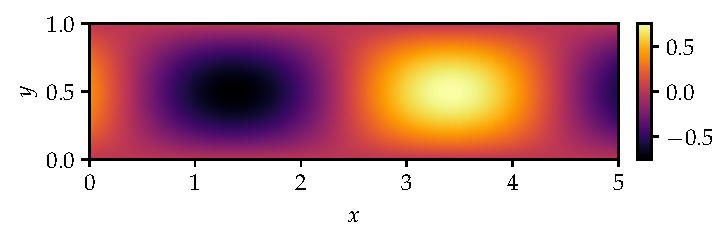
\includegraphics{plots/imperfect_conductor_solution.pdf}
    \caption{The solution $\mathbf{u}_z$ obtained with the \acrshort{FEM} at the
    frequency $\omega = 3.5$. Unlike in Figures \ref{fig:rectangular-cavity-mode1}
    and \ref{fig:rectangular-cavity-mode5}, the solution does no longer have to
    vanish at the imperfect boundary on the right-hand edge.}
    \label{fig:imperfect-conductor-solution}
\end{figure}

\begin{figure}[ht]
    \centering
    %% Creator: Matplotlib, PGF backend
%%
%% To include the figure in your LaTeX document, write
%%   \input{<filename>.pgf}
%%
%% Make sure the required packages are loaded in your preamble
%%   \usepackage{pgf}
%%
%% Also ensure that all the required font packages are loaded; for instance,
%% the lmodern package is sometimes necessary when using math font.
%%   \usepackage{lmodern}
%%
%% Figures using additional raster images can only be included by \input if
%% they are in the same directory as the main LaTeX file. For loading figures
%% from other directories you can use the `import` package
%%   \usepackage{import}
%%
%% and then include the figures with
%%   \import{<path to file>}{<filename>.pgf}
%%
%% Matplotlib used the following preamble
%%   \usepackage{fontspec}
%%   \setmainfont{DejaVuSans.ttf}[Path=\detokenize{C:/Users/Fabio/Anaconda3/Lib/site-packages/matplotlib/mpl-data/fonts/ttf/}]
%%   \setsansfont{DejaVuSans.ttf}[Path=\detokenize{C:/Users/Fabio/Anaconda3/Lib/site-packages/matplotlib/mpl-data/fonts/ttf/}]
%%   \setmonofont{DejaVuSansMono.ttf}[Path=\detokenize{C:/Users/Fabio/Anaconda3/Lib/site-packages/matplotlib/mpl-data/fonts/ttf/}]
%%
\begingroup%
\makeatletter%
\begin{pgfpicture}%
\pgfpathrectangle{\pgfpointorigin}{\pgfqpoint{5.159353in}{3.668486in}}%
\pgfusepath{use as bounding box, clip}%
\begin{pgfscope}%
\pgfsetbuttcap%
\pgfsetmiterjoin%
\pgfsetlinewidth{0.000000pt}%
\definecolor{currentstroke}{rgb}{1.000000,1.000000,1.000000}%
\pgfsetstrokecolor{currentstroke}%
\pgfsetstrokeopacity{0.000000}%
\pgfsetdash{}{0pt}%
\pgfpathmoveto{\pgfqpoint{0.000000in}{0.000000in}}%
\pgfpathlineto{\pgfqpoint{5.159353in}{0.000000in}}%
\pgfpathlineto{\pgfqpoint{5.159353in}{3.668486in}}%
\pgfpathlineto{\pgfqpoint{0.000000in}{3.668486in}}%
\pgfpathlineto{\pgfqpoint{0.000000in}{0.000000in}}%
\pgfpathclose%
\pgfusepath{}%
\end{pgfscope}%
\begin{pgfscope}%
\pgfsetbuttcap%
\pgfsetmiterjoin%
\definecolor{currentfill}{rgb}{1.000000,1.000000,1.000000}%
\pgfsetfillcolor{currentfill}%
\pgfsetlinewidth{0.000000pt}%
\definecolor{currentstroke}{rgb}{0.000000,0.000000,0.000000}%
\pgfsetstrokecolor{currentstroke}%
\pgfsetstrokeopacity{0.000000}%
\pgfsetdash{}{0pt}%
\pgfpathmoveto{\pgfqpoint{0.622917in}{2.195759in}}%
\pgfpathlineto{\pgfqpoint{4.924167in}{2.195759in}}%
\pgfpathlineto{\pgfqpoint{4.924167in}{3.568486in}}%
\pgfpathlineto{\pgfqpoint{0.622917in}{3.568486in}}%
\pgfpathlineto{\pgfqpoint{0.622917in}{2.195759in}}%
\pgfpathclose%
\pgfusepath{fill}%
\end{pgfscope}%
\begin{pgfscope}%
\pgfsetbuttcap%
\pgfsetroundjoin%
\definecolor{currentfill}{rgb}{0.000000,0.000000,0.000000}%
\pgfsetfillcolor{currentfill}%
\pgfsetlinewidth{0.803000pt}%
\definecolor{currentstroke}{rgb}{0.000000,0.000000,0.000000}%
\pgfsetstrokecolor{currentstroke}%
\pgfsetdash{}{0pt}%
\pgfsys@defobject{currentmarker}{\pgfqpoint{0.000000in}{-0.048611in}}{\pgfqpoint{0.000000in}{0.000000in}}{%
\pgfpathmoveto{\pgfqpoint{0.000000in}{0.000000in}}%
\pgfpathlineto{\pgfqpoint{0.000000in}{-0.048611in}}%
\pgfusepath{stroke,fill}%
}%
\begin{pgfscope}%
\pgfsys@transformshift{0.622917in}{2.195759in}%
\pgfsys@useobject{currentmarker}{}%
\end{pgfscope}%
\end{pgfscope}%
\begin{pgfscope}%
\pgfsetbuttcap%
\pgfsetroundjoin%
\definecolor{currentfill}{rgb}{0.000000,0.000000,0.000000}%
\pgfsetfillcolor{currentfill}%
\pgfsetlinewidth{0.803000pt}%
\definecolor{currentstroke}{rgb}{0.000000,0.000000,0.000000}%
\pgfsetstrokecolor{currentstroke}%
\pgfsetdash{}{0pt}%
\pgfsys@defobject{currentmarker}{\pgfqpoint{0.000000in}{-0.048611in}}{\pgfqpoint{0.000000in}{0.000000in}}{%
\pgfpathmoveto{\pgfqpoint{0.000000in}{0.000000in}}%
\pgfpathlineto{\pgfqpoint{0.000000in}{-0.048611in}}%
\pgfusepath{stroke,fill}%
}%
\begin{pgfscope}%
\pgfsys@transformshift{1.160574in}{2.195759in}%
\pgfsys@useobject{currentmarker}{}%
\end{pgfscope}%
\end{pgfscope}%
\begin{pgfscope}%
\pgfsetbuttcap%
\pgfsetroundjoin%
\definecolor{currentfill}{rgb}{0.000000,0.000000,0.000000}%
\pgfsetfillcolor{currentfill}%
\pgfsetlinewidth{0.803000pt}%
\definecolor{currentstroke}{rgb}{0.000000,0.000000,0.000000}%
\pgfsetstrokecolor{currentstroke}%
\pgfsetdash{}{0pt}%
\pgfsys@defobject{currentmarker}{\pgfqpoint{0.000000in}{-0.048611in}}{\pgfqpoint{0.000000in}{0.000000in}}{%
\pgfpathmoveto{\pgfqpoint{0.000000in}{0.000000in}}%
\pgfpathlineto{\pgfqpoint{0.000000in}{-0.048611in}}%
\pgfusepath{stroke,fill}%
}%
\begin{pgfscope}%
\pgfsys@transformshift{1.698230in}{2.195759in}%
\pgfsys@useobject{currentmarker}{}%
\end{pgfscope}%
\end{pgfscope}%
\begin{pgfscope}%
\pgfsetbuttcap%
\pgfsetroundjoin%
\definecolor{currentfill}{rgb}{0.000000,0.000000,0.000000}%
\pgfsetfillcolor{currentfill}%
\pgfsetlinewidth{0.803000pt}%
\definecolor{currentstroke}{rgb}{0.000000,0.000000,0.000000}%
\pgfsetstrokecolor{currentstroke}%
\pgfsetdash{}{0pt}%
\pgfsys@defobject{currentmarker}{\pgfqpoint{0.000000in}{-0.048611in}}{\pgfqpoint{0.000000in}{0.000000in}}{%
\pgfpathmoveto{\pgfqpoint{0.000000in}{0.000000in}}%
\pgfpathlineto{\pgfqpoint{0.000000in}{-0.048611in}}%
\pgfusepath{stroke,fill}%
}%
\begin{pgfscope}%
\pgfsys@transformshift{2.235886in}{2.195759in}%
\pgfsys@useobject{currentmarker}{}%
\end{pgfscope}%
\end{pgfscope}%
\begin{pgfscope}%
\pgfsetbuttcap%
\pgfsetroundjoin%
\definecolor{currentfill}{rgb}{0.000000,0.000000,0.000000}%
\pgfsetfillcolor{currentfill}%
\pgfsetlinewidth{0.803000pt}%
\definecolor{currentstroke}{rgb}{0.000000,0.000000,0.000000}%
\pgfsetstrokecolor{currentstroke}%
\pgfsetdash{}{0pt}%
\pgfsys@defobject{currentmarker}{\pgfqpoint{0.000000in}{-0.048611in}}{\pgfqpoint{0.000000in}{0.000000in}}{%
\pgfpathmoveto{\pgfqpoint{0.000000in}{0.000000in}}%
\pgfpathlineto{\pgfqpoint{0.000000in}{-0.048611in}}%
\pgfusepath{stroke,fill}%
}%
\begin{pgfscope}%
\pgfsys@transformshift{2.773543in}{2.195759in}%
\pgfsys@useobject{currentmarker}{}%
\end{pgfscope}%
\end{pgfscope}%
\begin{pgfscope}%
\pgfsetbuttcap%
\pgfsetroundjoin%
\definecolor{currentfill}{rgb}{0.000000,0.000000,0.000000}%
\pgfsetfillcolor{currentfill}%
\pgfsetlinewidth{0.803000pt}%
\definecolor{currentstroke}{rgb}{0.000000,0.000000,0.000000}%
\pgfsetstrokecolor{currentstroke}%
\pgfsetdash{}{0pt}%
\pgfsys@defobject{currentmarker}{\pgfqpoint{0.000000in}{-0.048611in}}{\pgfqpoint{0.000000in}{0.000000in}}{%
\pgfpathmoveto{\pgfqpoint{0.000000in}{0.000000in}}%
\pgfpathlineto{\pgfqpoint{0.000000in}{-0.048611in}}%
\pgfusepath{stroke,fill}%
}%
\begin{pgfscope}%
\pgfsys@transformshift{3.311199in}{2.195759in}%
\pgfsys@useobject{currentmarker}{}%
\end{pgfscope}%
\end{pgfscope}%
\begin{pgfscope}%
\pgfsetbuttcap%
\pgfsetroundjoin%
\definecolor{currentfill}{rgb}{0.000000,0.000000,0.000000}%
\pgfsetfillcolor{currentfill}%
\pgfsetlinewidth{0.803000pt}%
\definecolor{currentstroke}{rgb}{0.000000,0.000000,0.000000}%
\pgfsetstrokecolor{currentstroke}%
\pgfsetdash{}{0pt}%
\pgfsys@defobject{currentmarker}{\pgfqpoint{0.000000in}{-0.048611in}}{\pgfqpoint{0.000000in}{0.000000in}}{%
\pgfpathmoveto{\pgfqpoint{0.000000in}{0.000000in}}%
\pgfpathlineto{\pgfqpoint{0.000000in}{-0.048611in}}%
\pgfusepath{stroke,fill}%
}%
\begin{pgfscope}%
\pgfsys@transformshift{3.848855in}{2.195759in}%
\pgfsys@useobject{currentmarker}{}%
\end{pgfscope}%
\end{pgfscope}%
\begin{pgfscope}%
\pgfsetbuttcap%
\pgfsetroundjoin%
\definecolor{currentfill}{rgb}{0.000000,0.000000,0.000000}%
\pgfsetfillcolor{currentfill}%
\pgfsetlinewidth{0.803000pt}%
\definecolor{currentstroke}{rgb}{0.000000,0.000000,0.000000}%
\pgfsetstrokecolor{currentstroke}%
\pgfsetdash{}{0pt}%
\pgfsys@defobject{currentmarker}{\pgfqpoint{0.000000in}{-0.048611in}}{\pgfqpoint{0.000000in}{0.000000in}}{%
\pgfpathmoveto{\pgfqpoint{0.000000in}{0.000000in}}%
\pgfpathlineto{\pgfqpoint{0.000000in}{-0.048611in}}%
\pgfusepath{stroke,fill}%
}%
\begin{pgfscope}%
\pgfsys@transformshift{4.386511in}{2.195759in}%
\pgfsys@useobject{currentmarker}{}%
\end{pgfscope}%
\end{pgfscope}%
\begin{pgfscope}%
\pgfsetbuttcap%
\pgfsetroundjoin%
\definecolor{currentfill}{rgb}{0.000000,0.000000,0.000000}%
\pgfsetfillcolor{currentfill}%
\pgfsetlinewidth{0.803000pt}%
\definecolor{currentstroke}{rgb}{0.000000,0.000000,0.000000}%
\pgfsetstrokecolor{currentstroke}%
\pgfsetdash{}{0pt}%
\pgfsys@defobject{currentmarker}{\pgfqpoint{0.000000in}{-0.048611in}}{\pgfqpoint{0.000000in}{0.000000in}}{%
\pgfpathmoveto{\pgfqpoint{0.000000in}{0.000000in}}%
\pgfpathlineto{\pgfqpoint{0.000000in}{-0.048611in}}%
\pgfusepath{stroke,fill}%
}%
\begin{pgfscope}%
\pgfsys@transformshift{4.924168in}{2.195759in}%
\pgfsys@useobject{currentmarker}{}%
\end{pgfscope}%
\end{pgfscope}%
\begin{pgfscope}%
\pgfpathrectangle{\pgfqpoint{0.622917in}{2.195759in}}{\pgfqpoint{4.301250in}{1.372727in}}%
\pgfusepath{clip}%
\pgfsetrectcap%
\pgfsetroundjoin%
\pgfsetlinewidth{0.803000pt}%
\definecolor{currentstroke}{rgb}{0.690196,0.690196,0.690196}%
\pgfsetstrokecolor{currentstroke}%
\pgfsetdash{}{0pt}%
\pgfpathmoveto{\pgfqpoint{0.622917in}{2.518809in}}%
\pgfpathlineto{\pgfqpoint{4.924167in}{2.518809in}}%
\pgfusepath{stroke}%
\end{pgfscope}%
\begin{pgfscope}%
\pgfsetbuttcap%
\pgfsetroundjoin%
\definecolor{currentfill}{rgb}{0.000000,0.000000,0.000000}%
\pgfsetfillcolor{currentfill}%
\pgfsetlinewidth{0.803000pt}%
\definecolor{currentstroke}{rgb}{0.000000,0.000000,0.000000}%
\pgfsetstrokecolor{currentstroke}%
\pgfsetdash{}{0pt}%
\pgfsys@defobject{currentmarker}{\pgfqpoint{-0.048611in}{0.000000in}}{\pgfqpoint{-0.000000in}{0.000000in}}{%
\pgfpathmoveto{\pgfqpoint{-0.000000in}{0.000000in}}%
\pgfpathlineto{\pgfqpoint{-0.048611in}{0.000000in}}%
\pgfusepath{stroke,fill}%
}%
\begin{pgfscope}%
\pgfsys@transformshift{0.622917in}{2.518809in}%
\pgfsys@useobject{currentmarker}{}%
\end{pgfscope}%
\end{pgfscope}%
\begin{pgfscope}%
\definecolor{textcolor}{rgb}{0.000000,0.000000,0.000000}%
\pgfsetstrokecolor{textcolor}%
\pgfsetfillcolor{textcolor}%
\pgftext[x=0.307639in, y=2.460772in, left, base]{\color{textcolor}\rmfamily\fontsize{11.000000}{13.200000}\selectfont \(\displaystyle {10^{0}}\)}%
\end{pgfscope}%
\begin{pgfscope}%
\pgfpathrectangle{\pgfqpoint{0.622917in}{2.195759in}}{\pgfqpoint{4.301250in}{1.372727in}}%
\pgfusepath{clip}%
\pgfsetrectcap%
\pgfsetroundjoin%
\pgfsetlinewidth{0.803000pt}%
\definecolor{currentstroke}{rgb}{0.690196,0.690196,0.690196}%
\pgfsetstrokecolor{currentstroke}%
\pgfsetdash{}{0pt}%
\pgfpathmoveto{\pgfqpoint{0.622917in}{3.136640in}}%
\pgfpathlineto{\pgfqpoint{4.924167in}{3.136640in}}%
\pgfusepath{stroke}%
\end{pgfscope}%
\begin{pgfscope}%
\pgfsetbuttcap%
\pgfsetroundjoin%
\definecolor{currentfill}{rgb}{0.000000,0.000000,0.000000}%
\pgfsetfillcolor{currentfill}%
\pgfsetlinewidth{0.803000pt}%
\definecolor{currentstroke}{rgb}{0.000000,0.000000,0.000000}%
\pgfsetstrokecolor{currentstroke}%
\pgfsetdash{}{0pt}%
\pgfsys@defobject{currentmarker}{\pgfqpoint{-0.048611in}{0.000000in}}{\pgfqpoint{-0.000000in}{0.000000in}}{%
\pgfpathmoveto{\pgfqpoint{-0.000000in}{0.000000in}}%
\pgfpathlineto{\pgfqpoint{-0.048611in}{0.000000in}}%
\pgfusepath{stroke,fill}%
}%
\begin{pgfscope}%
\pgfsys@transformshift{0.622917in}{3.136640in}%
\pgfsys@useobject{currentmarker}{}%
\end{pgfscope}%
\end{pgfscope}%
\begin{pgfscope}%
\definecolor{textcolor}{rgb}{0.000000,0.000000,0.000000}%
\pgfsetstrokecolor{textcolor}%
\pgfsetfillcolor{textcolor}%
\pgftext[x=0.307639in, y=3.078603in, left, base]{\color{textcolor}\rmfamily\fontsize{11.000000}{13.200000}\selectfont \(\displaystyle {10^{1}}\)}%
\end{pgfscope}%
\begin{pgfscope}%
\pgfsetbuttcap%
\pgfsetroundjoin%
\definecolor{currentfill}{rgb}{0.000000,0.000000,0.000000}%
\pgfsetfillcolor{currentfill}%
\pgfsetlinewidth{0.602250pt}%
\definecolor{currentstroke}{rgb}{0.000000,0.000000,0.000000}%
\pgfsetstrokecolor{currentstroke}%
\pgfsetdash{}{0pt}%
\pgfsys@defobject{currentmarker}{\pgfqpoint{-0.027778in}{0.000000in}}{\pgfqpoint{-0.000000in}{0.000000in}}{%
\pgfpathmoveto{\pgfqpoint{-0.000000in}{0.000000in}}%
\pgfpathlineto{\pgfqpoint{-0.027778in}{0.000000in}}%
\pgfusepath{stroke,fill}%
}%
\begin{pgfscope}%
\pgfsys@transformshift{0.622917in}{2.195759in}%
\pgfsys@useobject{currentmarker}{}%
\end{pgfscope}%
\end{pgfscope}%
\begin{pgfscope}%
\pgfsetbuttcap%
\pgfsetroundjoin%
\definecolor{currentfill}{rgb}{0.000000,0.000000,0.000000}%
\pgfsetfillcolor{currentfill}%
\pgfsetlinewidth{0.602250pt}%
\definecolor{currentstroke}{rgb}{0.000000,0.000000,0.000000}%
\pgfsetstrokecolor{currentstroke}%
\pgfsetdash{}{0pt}%
\pgfsys@defobject{currentmarker}{\pgfqpoint{-0.027778in}{0.000000in}}{\pgfqpoint{-0.000000in}{0.000000in}}{%
\pgfpathmoveto{\pgfqpoint{-0.000000in}{0.000000in}}%
\pgfpathlineto{\pgfqpoint{-0.027778in}{0.000000in}}%
\pgfusepath{stroke,fill}%
}%
\begin{pgfscope}%
\pgfsys@transformshift{0.622917in}{2.272950in}%
\pgfsys@useobject{currentmarker}{}%
\end{pgfscope}%
\end{pgfscope}%
\begin{pgfscope}%
\pgfsetbuttcap%
\pgfsetroundjoin%
\definecolor{currentfill}{rgb}{0.000000,0.000000,0.000000}%
\pgfsetfillcolor{currentfill}%
\pgfsetlinewidth{0.602250pt}%
\definecolor{currentstroke}{rgb}{0.000000,0.000000,0.000000}%
\pgfsetstrokecolor{currentstroke}%
\pgfsetdash{}{0pt}%
\pgfsys@defobject{currentmarker}{\pgfqpoint{-0.027778in}{0.000000in}}{\pgfqpoint{-0.000000in}{0.000000in}}{%
\pgfpathmoveto{\pgfqpoint{-0.000000in}{0.000000in}}%
\pgfpathlineto{\pgfqpoint{-0.027778in}{0.000000in}}%
\pgfusepath{stroke,fill}%
}%
\begin{pgfscope}%
\pgfsys@transformshift{0.622917in}{2.332824in}%
\pgfsys@useobject{currentmarker}{}%
\end{pgfscope}%
\end{pgfscope}%
\begin{pgfscope}%
\pgfsetbuttcap%
\pgfsetroundjoin%
\definecolor{currentfill}{rgb}{0.000000,0.000000,0.000000}%
\pgfsetfillcolor{currentfill}%
\pgfsetlinewidth{0.602250pt}%
\definecolor{currentstroke}{rgb}{0.000000,0.000000,0.000000}%
\pgfsetstrokecolor{currentstroke}%
\pgfsetdash{}{0pt}%
\pgfsys@defobject{currentmarker}{\pgfqpoint{-0.027778in}{0.000000in}}{\pgfqpoint{-0.000000in}{0.000000in}}{%
\pgfpathmoveto{\pgfqpoint{-0.000000in}{0.000000in}}%
\pgfpathlineto{\pgfqpoint{-0.027778in}{0.000000in}}%
\pgfusepath{stroke,fill}%
}%
\begin{pgfscope}%
\pgfsys@transformshift{0.622917in}{2.381744in}%
\pgfsys@useobject{currentmarker}{}%
\end{pgfscope}%
\end{pgfscope}%
\begin{pgfscope}%
\pgfsetbuttcap%
\pgfsetroundjoin%
\definecolor{currentfill}{rgb}{0.000000,0.000000,0.000000}%
\pgfsetfillcolor{currentfill}%
\pgfsetlinewidth{0.602250pt}%
\definecolor{currentstroke}{rgb}{0.000000,0.000000,0.000000}%
\pgfsetstrokecolor{currentstroke}%
\pgfsetdash{}{0pt}%
\pgfsys@defobject{currentmarker}{\pgfqpoint{-0.027778in}{0.000000in}}{\pgfqpoint{-0.000000in}{0.000000in}}{%
\pgfpathmoveto{\pgfqpoint{-0.000000in}{0.000000in}}%
\pgfpathlineto{\pgfqpoint{-0.027778in}{0.000000in}}%
\pgfusepath{stroke,fill}%
}%
\begin{pgfscope}%
\pgfsys@transformshift{0.622917in}{2.423106in}%
\pgfsys@useobject{currentmarker}{}%
\end{pgfscope}%
\end{pgfscope}%
\begin{pgfscope}%
\pgfsetbuttcap%
\pgfsetroundjoin%
\definecolor{currentfill}{rgb}{0.000000,0.000000,0.000000}%
\pgfsetfillcolor{currentfill}%
\pgfsetlinewidth{0.602250pt}%
\definecolor{currentstroke}{rgb}{0.000000,0.000000,0.000000}%
\pgfsetstrokecolor{currentstroke}%
\pgfsetdash{}{0pt}%
\pgfsys@defobject{currentmarker}{\pgfqpoint{-0.027778in}{0.000000in}}{\pgfqpoint{-0.000000in}{0.000000in}}{%
\pgfpathmoveto{\pgfqpoint{-0.000000in}{0.000000in}}%
\pgfpathlineto{\pgfqpoint{-0.027778in}{0.000000in}}%
\pgfusepath{stroke,fill}%
}%
\begin{pgfscope}%
\pgfsys@transformshift{0.622917in}{2.458935in}%
\pgfsys@useobject{currentmarker}{}%
\end{pgfscope}%
\end{pgfscope}%
\begin{pgfscope}%
\pgfsetbuttcap%
\pgfsetroundjoin%
\definecolor{currentfill}{rgb}{0.000000,0.000000,0.000000}%
\pgfsetfillcolor{currentfill}%
\pgfsetlinewidth{0.602250pt}%
\definecolor{currentstroke}{rgb}{0.000000,0.000000,0.000000}%
\pgfsetstrokecolor{currentstroke}%
\pgfsetdash{}{0pt}%
\pgfsys@defobject{currentmarker}{\pgfqpoint{-0.027778in}{0.000000in}}{\pgfqpoint{-0.000000in}{0.000000in}}{%
\pgfpathmoveto{\pgfqpoint{-0.000000in}{0.000000in}}%
\pgfpathlineto{\pgfqpoint{-0.027778in}{0.000000in}}%
\pgfusepath{stroke,fill}%
}%
\begin{pgfscope}%
\pgfsys@transformshift{0.622917in}{2.490539in}%
\pgfsys@useobject{currentmarker}{}%
\end{pgfscope}%
\end{pgfscope}%
\begin{pgfscope}%
\pgfsetbuttcap%
\pgfsetroundjoin%
\definecolor{currentfill}{rgb}{0.000000,0.000000,0.000000}%
\pgfsetfillcolor{currentfill}%
\pgfsetlinewidth{0.602250pt}%
\definecolor{currentstroke}{rgb}{0.000000,0.000000,0.000000}%
\pgfsetstrokecolor{currentstroke}%
\pgfsetdash{}{0pt}%
\pgfsys@defobject{currentmarker}{\pgfqpoint{-0.027778in}{0.000000in}}{\pgfqpoint{-0.000000in}{0.000000in}}{%
\pgfpathmoveto{\pgfqpoint{-0.000000in}{0.000000in}}%
\pgfpathlineto{\pgfqpoint{-0.027778in}{0.000000in}}%
\pgfusepath{stroke,fill}%
}%
\begin{pgfscope}%
\pgfsys@transformshift{0.622917in}{2.704795in}%
\pgfsys@useobject{currentmarker}{}%
\end{pgfscope}%
\end{pgfscope}%
\begin{pgfscope}%
\pgfsetbuttcap%
\pgfsetroundjoin%
\definecolor{currentfill}{rgb}{0.000000,0.000000,0.000000}%
\pgfsetfillcolor{currentfill}%
\pgfsetlinewidth{0.602250pt}%
\definecolor{currentstroke}{rgb}{0.000000,0.000000,0.000000}%
\pgfsetstrokecolor{currentstroke}%
\pgfsetdash{}{0pt}%
\pgfsys@defobject{currentmarker}{\pgfqpoint{-0.027778in}{0.000000in}}{\pgfqpoint{-0.000000in}{0.000000in}}{%
\pgfpathmoveto{\pgfqpoint{-0.000000in}{0.000000in}}%
\pgfpathlineto{\pgfqpoint{-0.027778in}{0.000000in}}%
\pgfusepath{stroke,fill}%
}%
\begin{pgfscope}%
\pgfsys@transformshift{0.622917in}{2.813590in}%
\pgfsys@useobject{currentmarker}{}%
\end{pgfscope}%
\end{pgfscope}%
\begin{pgfscope}%
\pgfsetbuttcap%
\pgfsetroundjoin%
\definecolor{currentfill}{rgb}{0.000000,0.000000,0.000000}%
\pgfsetfillcolor{currentfill}%
\pgfsetlinewidth{0.602250pt}%
\definecolor{currentstroke}{rgb}{0.000000,0.000000,0.000000}%
\pgfsetstrokecolor{currentstroke}%
\pgfsetdash{}{0pt}%
\pgfsys@defobject{currentmarker}{\pgfqpoint{-0.027778in}{0.000000in}}{\pgfqpoint{-0.000000in}{0.000000in}}{%
\pgfpathmoveto{\pgfqpoint{-0.000000in}{0.000000in}}%
\pgfpathlineto{\pgfqpoint{-0.027778in}{0.000000in}}%
\pgfusepath{stroke,fill}%
}%
\begin{pgfscope}%
\pgfsys@transformshift{0.622917in}{2.890781in}%
\pgfsys@useobject{currentmarker}{}%
\end{pgfscope}%
\end{pgfscope}%
\begin{pgfscope}%
\pgfsetbuttcap%
\pgfsetroundjoin%
\definecolor{currentfill}{rgb}{0.000000,0.000000,0.000000}%
\pgfsetfillcolor{currentfill}%
\pgfsetlinewidth{0.602250pt}%
\definecolor{currentstroke}{rgb}{0.000000,0.000000,0.000000}%
\pgfsetstrokecolor{currentstroke}%
\pgfsetdash{}{0pt}%
\pgfsys@defobject{currentmarker}{\pgfqpoint{-0.027778in}{0.000000in}}{\pgfqpoint{-0.000000in}{0.000000in}}{%
\pgfpathmoveto{\pgfqpoint{-0.000000in}{0.000000in}}%
\pgfpathlineto{\pgfqpoint{-0.027778in}{0.000000in}}%
\pgfusepath{stroke,fill}%
}%
\begin{pgfscope}%
\pgfsys@transformshift{0.622917in}{2.950655in}%
\pgfsys@useobject{currentmarker}{}%
\end{pgfscope}%
\end{pgfscope}%
\begin{pgfscope}%
\pgfsetbuttcap%
\pgfsetroundjoin%
\definecolor{currentfill}{rgb}{0.000000,0.000000,0.000000}%
\pgfsetfillcolor{currentfill}%
\pgfsetlinewidth{0.602250pt}%
\definecolor{currentstroke}{rgb}{0.000000,0.000000,0.000000}%
\pgfsetstrokecolor{currentstroke}%
\pgfsetdash{}{0pt}%
\pgfsys@defobject{currentmarker}{\pgfqpoint{-0.027778in}{0.000000in}}{\pgfqpoint{-0.000000in}{0.000000in}}{%
\pgfpathmoveto{\pgfqpoint{-0.000000in}{0.000000in}}%
\pgfpathlineto{\pgfqpoint{-0.027778in}{0.000000in}}%
\pgfusepath{stroke,fill}%
}%
\begin{pgfscope}%
\pgfsys@transformshift{0.622917in}{2.999575in}%
\pgfsys@useobject{currentmarker}{}%
\end{pgfscope}%
\end{pgfscope}%
\begin{pgfscope}%
\pgfsetbuttcap%
\pgfsetroundjoin%
\definecolor{currentfill}{rgb}{0.000000,0.000000,0.000000}%
\pgfsetfillcolor{currentfill}%
\pgfsetlinewidth{0.602250pt}%
\definecolor{currentstroke}{rgb}{0.000000,0.000000,0.000000}%
\pgfsetstrokecolor{currentstroke}%
\pgfsetdash{}{0pt}%
\pgfsys@defobject{currentmarker}{\pgfqpoint{-0.027778in}{0.000000in}}{\pgfqpoint{-0.000000in}{0.000000in}}{%
\pgfpathmoveto{\pgfqpoint{-0.000000in}{0.000000in}}%
\pgfpathlineto{\pgfqpoint{-0.027778in}{0.000000in}}%
\pgfusepath{stroke,fill}%
}%
\begin{pgfscope}%
\pgfsys@transformshift{0.622917in}{3.040937in}%
\pgfsys@useobject{currentmarker}{}%
\end{pgfscope}%
\end{pgfscope}%
\begin{pgfscope}%
\pgfsetbuttcap%
\pgfsetroundjoin%
\definecolor{currentfill}{rgb}{0.000000,0.000000,0.000000}%
\pgfsetfillcolor{currentfill}%
\pgfsetlinewidth{0.602250pt}%
\definecolor{currentstroke}{rgb}{0.000000,0.000000,0.000000}%
\pgfsetstrokecolor{currentstroke}%
\pgfsetdash{}{0pt}%
\pgfsys@defobject{currentmarker}{\pgfqpoint{-0.027778in}{0.000000in}}{\pgfqpoint{-0.000000in}{0.000000in}}{%
\pgfpathmoveto{\pgfqpoint{-0.000000in}{0.000000in}}%
\pgfpathlineto{\pgfqpoint{-0.027778in}{0.000000in}}%
\pgfusepath{stroke,fill}%
}%
\begin{pgfscope}%
\pgfsys@transformshift{0.622917in}{3.076766in}%
\pgfsys@useobject{currentmarker}{}%
\end{pgfscope}%
\end{pgfscope}%
\begin{pgfscope}%
\pgfsetbuttcap%
\pgfsetroundjoin%
\definecolor{currentfill}{rgb}{0.000000,0.000000,0.000000}%
\pgfsetfillcolor{currentfill}%
\pgfsetlinewidth{0.602250pt}%
\definecolor{currentstroke}{rgb}{0.000000,0.000000,0.000000}%
\pgfsetstrokecolor{currentstroke}%
\pgfsetdash{}{0pt}%
\pgfsys@defobject{currentmarker}{\pgfqpoint{-0.027778in}{0.000000in}}{\pgfqpoint{-0.000000in}{0.000000in}}{%
\pgfpathmoveto{\pgfqpoint{-0.000000in}{0.000000in}}%
\pgfpathlineto{\pgfqpoint{-0.027778in}{0.000000in}}%
\pgfusepath{stroke,fill}%
}%
\begin{pgfscope}%
\pgfsys@transformshift{0.622917in}{3.108370in}%
\pgfsys@useobject{currentmarker}{}%
\end{pgfscope}%
\end{pgfscope}%
\begin{pgfscope}%
\pgfsetbuttcap%
\pgfsetroundjoin%
\definecolor{currentfill}{rgb}{0.000000,0.000000,0.000000}%
\pgfsetfillcolor{currentfill}%
\pgfsetlinewidth{0.602250pt}%
\definecolor{currentstroke}{rgb}{0.000000,0.000000,0.000000}%
\pgfsetstrokecolor{currentstroke}%
\pgfsetdash{}{0pt}%
\pgfsys@defobject{currentmarker}{\pgfqpoint{-0.027778in}{0.000000in}}{\pgfqpoint{-0.000000in}{0.000000in}}{%
\pgfpathmoveto{\pgfqpoint{-0.000000in}{0.000000in}}%
\pgfpathlineto{\pgfqpoint{-0.027778in}{0.000000in}}%
\pgfusepath{stroke,fill}%
}%
\begin{pgfscope}%
\pgfsys@transformshift{0.622917in}{3.322626in}%
\pgfsys@useobject{currentmarker}{}%
\end{pgfscope}%
\end{pgfscope}%
\begin{pgfscope}%
\pgfsetbuttcap%
\pgfsetroundjoin%
\definecolor{currentfill}{rgb}{0.000000,0.000000,0.000000}%
\pgfsetfillcolor{currentfill}%
\pgfsetlinewidth{0.602250pt}%
\definecolor{currentstroke}{rgb}{0.000000,0.000000,0.000000}%
\pgfsetstrokecolor{currentstroke}%
\pgfsetdash{}{0pt}%
\pgfsys@defobject{currentmarker}{\pgfqpoint{-0.027778in}{0.000000in}}{\pgfqpoint{-0.000000in}{0.000000in}}{%
\pgfpathmoveto{\pgfqpoint{-0.000000in}{0.000000in}}%
\pgfpathlineto{\pgfqpoint{-0.027778in}{0.000000in}}%
\pgfusepath{stroke,fill}%
}%
\begin{pgfscope}%
\pgfsys@transformshift{0.622917in}{3.431421in}%
\pgfsys@useobject{currentmarker}{}%
\end{pgfscope}%
\end{pgfscope}%
\begin{pgfscope}%
\pgfsetbuttcap%
\pgfsetroundjoin%
\definecolor{currentfill}{rgb}{0.000000,0.000000,0.000000}%
\pgfsetfillcolor{currentfill}%
\pgfsetlinewidth{0.602250pt}%
\definecolor{currentstroke}{rgb}{0.000000,0.000000,0.000000}%
\pgfsetstrokecolor{currentstroke}%
\pgfsetdash{}{0pt}%
\pgfsys@defobject{currentmarker}{\pgfqpoint{-0.027778in}{0.000000in}}{\pgfqpoint{-0.000000in}{0.000000in}}{%
\pgfpathmoveto{\pgfqpoint{-0.000000in}{0.000000in}}%
\pgfpathlineto{\pgfqpoint{-0.027778in}{0.000000in}}%
\pgfusepath{stroke,fill}%
}%
\begin{pgfscope}%
\pgfsys@transformshift{0.622917in}{3.508612in}%
\pgfsys@useobject{currentmarker}{}%
\end{pgfscope}%
\end{pgfscope}%
\begin{pgfscope}%
\pgfsetbuttcap%
\pgfsetroundjoin%
\definecolor{currentfill}{rgb}{0.000000,0.000000,0.000000}%
\pgfsetfillcolor{currentfill}%
\pgfsetlinewidth{0.602250pt}%
\definecolor{currentstroke}{rgb}{0.000000,0.000000,0.000000}%
\pgfsetstrokecolor{currentstroke}%
\pgfsetdash{}{0pt}%
\pgfsys@defobject{currentmarker}{\pgfqpoint{-0.027778in}{0.000000in}}{\pgfqpoint{-0.000000in}{0.000000in}}{%
\pgfpathmoveto{\pgfqpoint{-0.000000in}{0.000000in}}%
\pgfpathlineto{\pgfqpoint{-0.027778in}{0.000000in}}%
\pgfusepath{stroke,fill}%
}%
\begin{pgfscope}%
\pgfsys@transformshift{0.622917in}{3.568486in}%
\pgfsys@useobject{currentmarker}{}%
\end{pgfscope}%
\end{pgfscope}%
\begin{pgfscope}%
\definecolor{textcolor}{rgb}{0.000000,0.000000,0.000000}%
\pgfsetstrokecolor{textcolor}%
\pgfsetfillcolor{textcolor}%
\pgftext[x=0.252083in,y=2.882122in,,bottom,rotate=90.000000]{\color{textcolor}\rmfamily\fontsize{11.000000}{13.200000}\selectfont \(\displaystyle ||\mathbf{u}_z(\omega)||_M\)}%
\end{pgfscope}%
\begin{pgfscope}%
\pgfpathrectangle{\pgfqpoint{0.622917in}{2.195759in}}{\pgfqpoint{4.301250in}{1.372727in}}%
\pgfusepath{clip}%
\pgfsetrectcap%
\pgfsetroundjoin%
\pgfsetlinewidth{1.505625pt}%
\definecolor{currentstroke}{rgb}{0.001462,0.000466,0.013866}%
\pgfsetstrokecolor{currentstroke}%
\pgfsetdash{}{0pt}%
\pgfpathmoveto{\pgfqpoint{0.622917in}{2.357393in}}%
\pgfpathlineto{\pgfqpoint{0.661668in}{2.383657in}}%
\pgfpathlineto{\pgfqpoint{0.696112in}{2.410373in}}%
\pgfpathlineto{\pgfqpoint{0.730556in}{2.441241in}}%
\pgfpathlineto{\pgfqpoint{0.760695in}{2.472757in}}%
\pgfpathlineto{\pgfqpoint{0.786529in}{2.504243in}}%
\pgfpathlineto{\pgfqpoint{0.808056in}{2.534661in}}%
\pgfpathlineto{\pgfqpoint{0.829584in}{2.570134in}}%
\pgfpathlineto{\pgfqpoint{0.851112in}{2.612488in}}%
\pgfpathlineto{\pgfqpoint{0.868334in}{2.653259in}}%
\pgfpathlineto{\pgfqpoint{0.885556in}{2.702795in}}%
\pgfpathlineto{\pgfqpoint{0.898473in}{2.748177in}}%
\pgfpathlineto{\pgfqpoint{0.911390in}{2.803966in}}%
\pgfpathlineto{\pgfqpoint{0.924306in}{2.875823in}}%
\pgfpathlineto{\pgfqpoint{0.932917in}{2.938027in}}%
\pgfpathlineto{\pgfqpoint{0.941529in}{3.019539in}}%
\pgfpathlineto{\pgfqpoint{0.950140in}{3.136266in}}%
\pgfpathlineto{\pgfqpoint{0.958751in}{3.329895in}}%
\pgfpathlineto{\pgfqpoint{0.963056in}{3.457811in}}%
\pgfpathlineto{\pgfqpoint{0.967362in}{3.439334in}}%
\pgfpathlineto{\pgfqpoint{0.975973in}{3.203524in}}%
\pgfpathlineto{\pgfqpoint{0.984584in}{3.062729in}}%
\pgfpathlineto{\pgfqpoint{0.993195in}{2.969988in}}%
\pgfpathlineto{\pgfqpoint{1.006112in}{2.873909in}}%
\pgfpathlineto{\pgfqpoint{1.019029in}{2.806187in}}%
\pgfpathlineto{\pgfqpoint{1.031945in}{2.755896in}}%
\pgfpathlineto{\pgfqpoint{1.044862in}{2.718066in}}%
\pgfpathlineto{\pgfqpoint{1.057779in}{2.690148in}}%
\pgfpathlineto{\pgfqpoint{1.070695in}{2.670757in}}%
\pgfpathlineto{\pgfqpoint{1.079306in}{2.662162in}}%
\pgfpathlineto{\pgfqpoint{1.087918in}{2.656856in}}%
\pgfpathlineto{\pgfqpoint{1.096529in}{2.654732in}}%
\pgfpathlineto{\pgfqpoint{1.105140in}{2.655714in}}%
\pgfpathlineto{\pgfqpoint{1.113751in}{2.659746in}}%
\pgfpathlineto{\pgfqpoint{1.122362in}{2.666789in}}%
\pgfpathlineto{\pgfqpoint{1.135279in}{2.682949in}}%
\pgfpathlineto{\pgfqpoint{1.148195in}{2.705810in}}%
\pgfpathlineto{\pgfqpoint{1.161112in}{2.735369in}}%
\pgfpathlineto{\pgfqpoint{1.178334in}{2.784809in}}%
\pgfpathlineto{\pgfqpoint{1.212779in}{2.894076in}}%
\pgfpathlineto{\pgfqpoint{1.221390in}{2.907717in}}%
\pgfpathlineto{\pgfqpoint{1.225695in}{2.909558in}}%
\pgfpathlineto{\pgfqpoint{1.230001in}{2.907773in}}%
\pgfpathlineto{\pgfqpoint{1.234306in}{2.902501in}}%
\pgfpathlineto{\pgfqpoint{1.242918in}{2.883273in}}%
\pgfpathlineto{\pgfqpoint{1.255834in}{2.841671in}}%
\pgfpathlineto{\pgfqpoint{1.285973in}{2.739911in}}%
\pgfpathlineto{\pgfqpoint{1.303195in}{2.691696in}}%
\pgfpathlineto{\pgfqpoint{1.320418in}{2.651230in}}%
\pgfpathlineto{\pgfqpoint{1.337640in}{2.617375in}}%
\pgfpathlineto{\pgfqpoint{1.354862in}{2.589072in}}%
\pgfpathlineto{\pgfqpoint{1.372084in}{2.565493in}}%
\pgfpathlineto{\pgfqpoint{1.393612in}{2.541751in}}%
\pgfpathlineto{\pgfqpoint{1.410834in}{2.526825in}}%
\pgfpathlineto{\pgfqpoint{1.428056in}{2.515196in}}%
\pgfpathlineto{\pgfqpoint{1.445279in}{2.506664in}}%
\pgfpathlineto{\pgfqpoint{1.462501in}{2.501093in}}%
\pgfpathlineto{\pgfqpoint{1.479723in}{2.498394in}}%
\pgfpathlineto{\pgfqpoint{1.496945in}{2.498508in}}%
\pgfpathlineto{\pgfqpoint{1.514168in}{2.501397in}}%
\pgfpathlineto{\pgfqpoint{1.531390in}{2.507032in}}%
\pgfpathlineto{\pgfqpoint{1.548612in}{2.515385in}}%
\pgfpathlineto{\pgfqpoint{1.570140in}{2.529574in}}%
\pgfpathlineto{\pgfqpoint{1.591667in}{2.547748in}}%
\pgfpathlineto{\pgfqpoint{1.617501in}{2.574222in}}%
\pgfpathlineto{\pgfqpoint{1.690695in}{2.654849in}}%
\pgfpathlineto{\pgfqpoint{1.703612in}{2.663124in}}%
\pgfpathlineto{\pgfqpoint{1.716529in}{2.667183in}}%
\pgfpathlineto{\pgfqpoint{1.725140in}{2.667264in}}%
\pgfpathlineto{\pgfqpoint{1.733751in}{2.665203in}}%
\pgfpathlineto{\pgfqpoint{1.746668in}{2.658339in}}%
\pgfpathlineto{\pgfqpoint{1.759584in}{2.647619in}}%
\pgfpathlineto{\pgfqpoint{1.776806in}{2.629038in}}%
\pgfpathlineto{\pgfqpoint{1.811251in}{2.585412in}}%
\pgfpathlineto{\pgfqpoint{1.850001in}{2.537491in}}%
\pgfpathlineto{\pgfqpoint{1.880140in}{2.505072in}}%
\pgfpathlineto{\pgfqpoint{1.910279in}{2.477654in}}%
\pgfpathlineto{\pgfqpoint{1.936112in}{2.458066in}}%
\pgfpathlineto{\pgfqpoint{1.961945in}{2.441904in}}%
\pgfpathlineto{\pgfqpoint{1.987779in}{2.428983in}}%
\pgfpathlineto{\pgfqpoint{2.013612in}{2.419138in}}%
\pgfpathlineto{\pgfqpoint{2.039445in}{2.412238in}}%
\pgfpathlineto{\pgfqpoint{2.065279in}{2.408178in}}%
\pgfpathlineto{\pgfqpoint{2.091112in}{2.406876in}}%
\pgfpathlineto{\pgfqpoint{2.116945in}{2.408263in}}%
\pgfpathlineto{\pgfqpoint{2.147084in}{2.413181in}}%
\pgfpathlineto{\pgfqpoint{2.177223in}{2.421516in}}%
\pgfpathlineto{\pgfqpoint{2.207362in}{2.433043in}}%
\pgfpathlineto{\pgfqpoint{2.241806in}{2.449631in}}%
\pgfpathlineto{\pgfqpoint{2.289168in}{2.476464in}}%
\pgfpathlineto{\pgfqpoint{2.340834in}{2.505289in}}%
\pgfpathlineto{\pgfqpoint{2.366668in}{2.516235in}}%
\pgfpathlineto{\pgfqpoint{2.388195in}{2.522036in}}%
\pgfpathlineto{\pgfqpoint{2.405417in}{2.523969in}}%
\pgfpathlineto{\pgfqpoint{2.422640in}{2.523278in}}%
\pgfpathlineto{\pgfqpoint{2.439862in}{2.519977in}}%
\pgfpathlineto{\pgfqpoint{2.461390in}{2.512509in}}%
\pgfpathlineto{\pgfqpoint{2.487223in}{2.499629in}}%
\pgfpathlineto{\pgfqpoint{2.521667in}{2.478299in}}%
\pgfpathlineto{\pgfqpoint{2.625001in}{2.411744in}}%
\pgfpathlineto{\pgfqpoint{2.663751in}{2.391341in}}%
\pgfpathlineto{\pgfqpoint{2.702501in}{2.374502in}}%
\pgfpathlineto{\pgfqpoint{2.741251in}{2.361338in}}%
\pgfpathlineto{\pgfqpoint{2.775695in}{2.352708in}}%
\pgfpathlineto{\pgfqpoint{2.810140in}{2.346919in}}%
\pgfpathlineto{\pgfqpoint{2.848890in}{2.343718in}}%
\pgfpathlineto{\pgfqpoint{2.887640in}{2.343917in}}%
\pgfpathlineto{\pgfqpoint{2.926390in}{2.347368in}}%
\pgfpathlineto{\pgfqpoint{2.965140in}{2.353863in}}%
\pgfpathlineto{\pgfqpoint{3.008195in}{2.364254in}}%
\pgfpathlineto{\pgfqpoint{3.059862in}{2.380141in}}%
\pgfpathlineto{\pgfqpoint{3.171806in}{2.416246in}}%
\pgfpathlineto{\pgfqpoint{3.206251in}{2.423359in}}%
\pgfpathlineto{\pgfqpoint{3.236390in}{2.426377in}}%
\pgfpathlineto{\pgfqpoint{3.266529in}{2.425912in}}%
\pgfpathlineto{\pgfqpoint{3.296667in}{2.421917in}}%
\pgfpathlineto{\pgfqpoint{3.326806in}{2.414755in}}%
\pgfpathlineto{\pgfqpoint{3.365556in}{2.401984in}}%
\pgfpathlineto{\pgfqpoint{3.421529in}{2.379646in}}%
\pgfpathlineto{\pgfqpoint{3.516251in}{2.341831in}}%
\pgfpathlineto{\pgfqpoint{3.567918in}{2.324708in}}%
\pgfpathlineto{\pgfqpoint{3.615279in}{2.312147in}}%
\pgfpathlineto{\pgfqpoint{3.662640in}{2.302841in}}%
\pgfpathlineto{\pgfqpoint{3.710001in}{2.296868in}}%
\pgfpathlineto{\pgfqpoint{3.757362in}{2.294204in}}%
\pgfpathlineto{\pgfqpoint{3.804723in}{2.294744in}}%
\pgfpathlineto{\pgfqpoint{3.852084in}{2.298295in}}%
\pgfpathlineto{\pgfqpoint{3.903751in}{2.305236in}}%
\pgfpathlineto{\pgfqpoint{3.964029in}{2.316531in}}%
\pgfpathlineto{\pgfqpoint{4.127640in}{2.349523in}}%
\pgfpathlineto{\pgfqpoint{4.170695in}{2.353745in}}%
\pgfpathlineto{\pgfqpoint{4.209445in}{2.354410in}}%
\pgfpathlineto{\pgfqpoint{4.248195in}{2.351870in}}%
\pgfpathlineto{\pgfqpoint{4.286945in}{2.346319in}}%
\pgfpathlineto{\pgfqpoint{4.334306in}{2.336240in}}%
\pgfpathlineto{\pgfqpoint{4.398890in}{2.318982in}}%
\pgfpathlineto{\pgfqpoint{4.528056in}{2.283938in}}%
\pgfpathlineto{\pgfqpoint{4.588334in}{2.270998in}}%
\pgfpathlineto{\pgfqpoint{4.644306in}{2.261942in}}%
\pgfpathlineto{\pgfqpoint{4.700279in}{2.255996in}}%
\pgfpathlineto{\pgfqpoint{4.756251in}{2.253224in}}%
\pgfpathlineto{\pgfqpoint{4.812223in}{2.253545in}}%
\pgfpathlineto{\pgfqpoint{4.872501in}{2.257084in}}%
\pgfpathlineto{\pgfqpoint{4.924168in}{2.262385in}}%
\pgfpathlineto{\pgfqpoint{4.924168in}{2.262385in}}%
\pgfusepath{stroke}%
\end{pgfscope}%
\begin{pgfscope}%
\pgfsetrectcap%
\pgfsetmiterjoin%
\pgfsetlinewidth{0.803000pt}%
\definecolor{currentstroke}{rgb}{0.000000,0.000000,0.000000}%
\pgfsetstrokecolor{currentstroke}%
\pgfsetdash{}{0pt}%
\pgfpathmoveto{\pgfqpoint{0.622917in}{2.195759in}}%
\pgfpathlineto{\pgfqpoint{0.622917in}{3.568486in}}%
\pgfusepath{stroke}%
\end{pgfscope}%
\begin{pgfscope}%
\pgfsetrectcap%
\pgfsetmiterjoin%
\pgfsetlinewidth{0.803000pt}%
\definecolor{currentstroke}{rgb}{0.000000,0.000000,0.000000}%
\pgfsetstrokecolor{currentstroke}%
\pgfsetdash{}{0pt}%
\pgfpathmoveto{\pgfqpoint{4.924167in}{2.195759in}}%
\pgfpathlineto{\pgfqpoint{4.924167in}{3.568486in}}%
\pgfusepath{stroke}%
\end{pgfscope}%
\begin{pgfscope}%
\pgfsetrectcap%
\pgfsetmiterjoin%
\pgfsetlinewidth{0.803000pt}%
\definecolor{currentstroke}{rgb}{0.000000,0.000000,0.000000}%
\pgfsetstrokecolor{currentstroke}%
\pgfsetdash{}{0pt}%
\pgfpathmoveto{\pgfqpoint{0.622917in}{2.195759in}}%
\pgfpathlineto{\pgfqpoint{4.924168in}{2.195759in}}%
\pgfusepath{stroke}%
\end{pgfscope}%
\begin{pgfscope}%
\pgfsetrectcap%
\pgfsetmiterjoin%
\pgfsetlinewidth{0.803000pt}%
\definecolor{currentstroke}{rgb}{0.000000,0.000000,0.000000}%
\pgfsetstrokecolor{currentstroke}%
\pgfsetdash{}{0pt}%
\pgfpathmoveto{\pgfqpoint{0.622917in}{3.568486in}}%
\pgfpathlineto{\pgfqpoint{4.924168in}{3.568486in}}%
\pgfusepath{stroke}%
\end{pgfscope}%
\begin{pgfscope}%
\pgfsetbuttcap%
\pgfsetmiterjoin%
\definecolor{currentfill}{rgb}{1.000000,1.000000,1.000000}%
\pgfsetfillcolor{currentfill}%
\pgfsetlinewidth{0.000000pt}%
\definecolor{currentstroke}{rgb}{0.000000,0.000000,0.000000}%
\pgfsetstrokecolor{currentstroke}%
\pgfsetstrokeopacity{0.000000}%
\pgfsetdash{}{0pt}%
\pgfpathmoveto{\pgfqpoint{0.622917in}{0.823031in}}%
\pgfpathlineto{\pgfqpoint{4.924167in}{0.823031in}}%
\pgfpathlineto{\pgfqpoint{4.924167in}{2.195759in}}%
\pgfpathlineto{\pgfqpoint{0.622917in}{2.195759in}}%
\pgfpathlineto{\pgfqpoint{0.622917in}{0.823031in}}%
\pgfpathclose%
\pgfusepath{fill}%
\end{pgfscope}%
\begin{pgfscope}%
\pgfsetbuttcap%
\pgfsetroundjoin%
\definecolor{currentfill}{rgb}{0.000000,0.000000,0.000000}%
\pgfsetfillcolor{currentfill}%
\pgfsetlinewidth{0.803000pt}%
\definecolor{currentstroke}{rgb}{0.000000,0.000000,0.000000}%
\pgfsetstrokecolor{currentstroke}%
\pgfsetdash{}{0pt}%
\pgfsys@defobject{currentmarker}{\pgfqpoint{0.000000in}{-0.048611in}}{\pgfqpoint{0.000000in}{0.000000in}}{%
\pgfpathmoveto{\pgfqpoint{0.000000in}{0.000000in}}%
\pgfpathlineto{\pgfqpoint{0.000000in}{-0.048611in}}%
\pgfusepath{stroke,fill}%
}%
\begin{pgfscope}%
\pgfsys@transformshift{0.622917in}{0.823031in}%
\pgfsys@useobject{currentmarker}{}%
\end{pgfscope}%
\end{pgfscope}%
\begin{pgfscope}%
\pgfsetbuttcap%
\pgfsetroundjoin%
\definecolor{currentfill}{rgb}{0.000000,0.000000,0.000000}%
\pgfsetfillcolor{currentfill}%
\pgfsetlinewidth{0.803000pt}%
\definecolor{currentstroke}{rgb}{0.000000,0.000000,0.000000}%
\pgfsetstrokecolor{currentstroke}%
\pgfsetdash{}{0pt}%
\pgfsys@defobject{currentmarker}{\pgfqpoint{0.000000in}{-0.048611in}}{\pgfqpoint{0.000000in}{0.000000in}}{%
\pgfpathmoveto{\pgfqpoint{0.000000in}{0.000000in}}%
\pgfpathlineto{\pgfqpoint{0.000000in}{-0.048611in}}%
\pgfusepath{stroke,fill}%
}%
\begin{pgfscope}%
\pgfsys@transformshift{1.160574in}{0.823031in}%
\pgfsys@useobject{currentmarker}{}%
\end{pgfscope}%
\end{pgfscope}%
\begin{pgfscope}%
\pgfsetbuttcap%
\pgfsetroundjoin%
\definecolor{currentfill}{rgb}{0.000000,0.000000,0.000000}%
\pgfsetfillcolor{currentfill}%
\pgfsetlinewidth{0.803000pt}%
\definecolor{currentstroke}{rgb}{0.000000,0.000000,0.000000}%
\pgfsetstrokecolor{currentstroke}%
\pgfsetdash{}{0pt}%
\pgfsys@defobject{currentmarker}{\pgfqpoint{0.000000in}{-0.048611in}}{\pgfqpoint{0.000000in}{0.000000in}}{%
\pgfpathmoveto{\pgfqpoint{0.000000in}{0.000000in}}%
\pgfpathlineto{\pgfqpoint{0.000000in}{-0.048611in}}%
\pgfusepath{stroke,fill}%
}%
\begin{pgfscope}%
\pgfsys@transformshift{1.698230in}{0.823031in}%
\pgfsys@useobject{currentmarker}{}%
\end{pgfscope}%
\end{pgfscope}%
\begin{pgfscope}%
\pgfsetbuttcap%
\pgfsetroundjoin%
\definecolor{currentfill}{rgb}{0.000000,0.000000,0.000000}%
\pgfsetfillcolor{currentfill}%
\pgfsetlinewidth{0.803000pt}%
\definecolor{currentstroke}{rgb}{0.000000,0.000000,0.000000}%
\pgfsetstrokecolor{currentstroke}%
\pgfsetdash{}{0pt}%
\pgfsys@defobject{currentmarker}{\pgfqpoint{0.000000in}{-0.048611in}}{\pgfqpoint{0.000000in}{0.000000in}}{%
\pgfpathmoveto{\pgfqpoint{0.000000in}{0.000000in}}%
\pgfpathlineto{\pgfqpoint{0.000000in}{-0.048611in}}%
\pgfusepath{stroke,fill}%
}%
\begin{pgfscope}%
\pgfsys@transformshift{2.235886in}{0.823031in}%
\pgfsys@useobject{currentmarker}{}%
\end{pgfscope}%
\end{pgfscope}%
\begin{pgfscope}%
\pgfsetbuttcap%
\pgfsetroundjoin%
\definecolor{currentfill}{rgb}{0.000000,0.000000,0.000000}%
\pgfsetfillcolor{currentfill}%
\pgfsetlinewidth{0.803000pt}%
\definecolor{currentstroke}{rgb}{0.000000,0.000000,0.000000}%
\pgfsetstrokecolor{currentstroke}%
\pgfsetdash{}{0pt}%
\pgfsys@defobject{currentmarker}{\pgfqpoint{0.000000in}{-0.048611in}}{\pgfqpoint{0.000000in}{0.000000in}}{%
\pgfpathmoveto{\pgfqpoint{0.000000in}{0.000000in}}%
\pgfpathlineto{\pgfqpoint{0.000000in}{-0.048611in}}%
\pgfusepath{stroke,fill}%
}%
\begin{pgfscope}%
\pgfsys@transformshift{2.773543in}{0.823031in}%
\pgfsys@useobject{currentmarker}{}%
\end{pgfscope}%
\end{pgfscope}%
\begin{pgfscope}%
\pgfsetbuttcap%
\pgfsetroundjoin%
\definecolor{currentfill}{rgb}{0.000000,0.000000,0.000000}%
\pgfsetfillcolor{currentfill}%
\pgfsetlinewidth{0.803000pt}%
\definecolor{currentstroke}{rgb}{0.000000,0.000000,0.000000}%
\pgfsetstrokecolor{currentstroke}%
\pgfsetdash{}{0pt}%
\pgfsys@defobject{currentmarker}{\pgfqpoint{0.000000in}{-0.048611in}}{\pgfqpoint{0.000000in}{0.000000in}}{%
\pgfpathmoveto{\pgfqpoint{0.000000in}{0.000000in}}%
\pgfpathlineto{\pgfqpoint{0.000000in}{-0.048611in}}%
\pgfusepath{stroke,fill}%
}%
\begin{pgfscope}%
\pgfsys@transformshift{3.311199in}{0.823031in}%
\pgfsys@useobject{currentmarker}{}%
\end{pgfscope}%
\end{pgfscope}%
\begin{pgfscope}%
\pgfsetbuttcap%
\pgfsetroundjoin%
\definecolor{currentfill}{rgb}{0.000000,0.000000,0.000000}%
\pgfsetfillcolor{currentfill}%
\pgfsetlinewidth{0.803000pt}%
\definecolor{currentstroke}{rgb}{0.000000,0.000000,0.000000}%
\pgfsetstrokecolor{currentstroke}%
\pgfsetdash{}{0pt}%
\pgfsys@defobject{currentmarker}{\pgfqpoint{0.000000in}{-0.048611in}}{\pgfqpoint{0.000000in}{0.000000in}}{%
\pgfpathmoveto{\pgfqpoint{0.000000in}{0.000000in}}%
\pgfpathlineto{\pgfqpoint{0.000000in}{-0.048611in}}%
\pgfusepath{stroke,fill}%
}%
\begin{pgfscope}%
\pgfsys@transformshift{3.848855in}{0.823031in}%
\pgfsys@useobject{currentmarker}{}%
\end{pgfscope}%
\end{pgfscope}%
\begin{pgfscope}%
\pgfsetbuttcap%
\pgfsetroundjoin%
\definecolor{currentfill}{rgb}{0.000000,0.000000,0.000000}%
\pgfsetfillcolor{currentfill}%
\pgfsetlinewidth{0.803000pt}%
\definecolor{currentstroke}{rgb}{0.000000,0.000000,0.000000}%
\pgfsetstrokecolor{currentstroke}%
\pgfsetdash{}{0pt}%
\pgfsys@defobject{currentmarker}{\pgfqpoint{0.000000in}{-0.048611in}}{\pgfqpoint{0.000000in}{0.000000in}}{%
\pgfpathmoveto{\pgfqpoint{0.000000in}{0.000000in}}%
\pgfpathlineto{\pgfqpoint{0.000000in}{-0.048611in}}%
\pgfusepath{stroke,fill}%
}%
\begin{pgfscope}%
\pgfsys@transformshift{4.386511in}{0.823031in}%
\pgfsys@useobject{currentmarker}{}%
\end{pgfscope}%
\end{pgfscope}%
\begin{pgfscope}%
\pgfsetbuttcap%
\pgfsetroundjoin%
\definecolor{currentfill}{rgb}{0.000000,0.000000,0.000000}%
\pgfsetfillcolor{currentfill}%
\pgfsetlinewidth{0.803000pt}%
\definecolor{currentstroke}{rgb}{0.000000,0.000000,0.000000}%
\pgfsetstrokecolor{currentstroke}%
\pgfsetdash{}{0pt}%
\pgfsys@defobject{currentmarker}{\pgfqpoint{0.000000in}{-0.048611in}}{\pgfqpoint{0.000000in}{0.000000in}}{%
\pgfpathmoveto{\pgfqpoint{0.000000in}{0.000000in}}%
\pgfpathlineto{\pgfqpoint{0.000000in}{-0.048611in}}%
\pgfusepath{stroke,fill}%
}%
\begin{pgfscope}%
\pgfsys@transformshift{4.924168in}{0.823031in}%
\pgfsys@useobject{currentmarker}{}%
\end{pgfscope}%
\end{pgfscope}%
\begin{pgfscope}%
\pgfpathrectangle{\pgfqpoint{0.622917in}{0.823031in}}{\pgfqpoint{4.301250in}{1.372727in}}%
\pgfusepath{clip}%
\pgfsetrectcap%
\pgfsetroundjoin%
\pgfsetlinewidth{0.803000pt}%
\definecolor{currentstroke}{rgb}{0.690196,0.690196,0.690196}%
\pgfsetstrokecolor{currentstroke}%
\pgfsetdash{}{0pt}%
\pgfpathmoveto{\pgfqpoint{0.622917in}{1.146082in}}%
\pgfpathlineto{\pgfqpoint{4.924167in}{1.146082in}}%
\pgfusepath{stroke}%
\end{pgfscope}%
\begin{pgfscope}%
\pgfsetbuttcap%
\pgfsetroundjoin%
\definecolor{currentfill}{rgb}{0.000000,0.000000,0.000000}%
\pgfsetfillcolor{currentfill}%
\pgfsetlinewidth{0.803000pt}%
\definecolor{currentstroke}{rgb}{0.000000,0.000000,0.000000}%
\pgfsetstrokecolor{currentstroke}%
\pgfsetdash{}{0pt}%
\pgfsys@defobject{currentmarker}{\pgfqpoint{-0.048611in}{0.000000in}}{\pgfqpoint{-0.000000in}{0.000000in}}{%
\pgfpathmoveto{\pgfqpoint{-0.000000in}{0.000000in}}%
\pgfpathlineto{\pgfqpoint{-0.048611in}{0.000000in}}%
\pgfusepath{stroke,fill}%
}%
\begin{pgfscope}%
\pgfsys@transformshift{0.622917in}{1.146082in}%
\pgfsys@useobject{currentmarker}{}%
\end{pgfscope}%
\end{pgfscope}%
\begin{pgfscope}%
\definecolor{textcolor}{rgb}{0.000000,0.000000,0.000000}%
\pgfsetstrokecolor{textcolor}%
\pgfsetfillcolor{textcolor}%
\pgftext[x=0.307639in, y=1.088044in, left, base]{\color{textcolor}\rmfamily\fontsize{11.000000}{13.200000}\selectfont \(\displaystyle {10^{0}}\)}%
\end{pgfscope}%
\begin{pgfscope}%
\pgfpathrectangle{\pgfqpoint{0.622917in}{0.823031in}}{\pgfqpoint{4.301250in}{1.372727in}}%
\pgfusepath{clip}%
\pgfsetrectcap%
\pgfsetroundjoin%
\pgfsetlinewidth{0.803000pt}%
\definecolor{currentstroke}{rgb}{0.690196,0.690196,0.690196}%
\pgfsetstrokecolor{currentstroke}%
\pgfsetdash{}{0pt}%
\pgfpathmoveto{\pgfqpoint{0.622917in}{1.763913in}}%
\pgfpathlineto{\pgfqpoint{4.924167in}{1.763913in}}%
\pgfusepath{stroke}%
\end{pgfscope}%
\begin{pgfscope}%
\pgfsetbuttcap%
\pgfsetroundjoin%
\definecolor{currentfill}{rgb}{0.000000,0.000000,0.000000}%
\pgfsetfillcolor{currentfill}%
\pgfsetlinewidth{0.803000pt}%
\definecolor{currentstroke}{rgb}{0.000000,0.000000,0.000000}%
\pgfsetstrokecolor{currentstroke}%
\pgfsetdash{}{0pt}%
\pgfsys@defobject{currentmarker}{\pgfqpoint{-0.048611in}{0.000000in}}{\pgfqpoint{-0.000000in}{0.000000in}}{%
\pgfpathmoveto{\pgfqpoint{-0.000000in}{0.000000in}}%
\pgfpathlineto{\pgfqpoint{-0.048611in}{0.000000in}}%
\pgfusepath{stroke,fill}%
}%
\begin{pgfscope}%
\pgfsys@transformshift{0.622917in}{1.763913in}%
\pgfsys@useobject{currentmarker}{}%
\end{pgfscope}%
\end{pgfscope}%
\begin{pgfscope}%
\definecolor{textcolor}{rgb}{0.000000,0.000000,0.000000}%
\pgfsetstrokecolor{textcolor}%
\pgfsetfillcolor{textcolor}%
\pgftext[x=0.307639in, y=1.705876in, left, base]{\color{textcolor}\rmfamily\fontsize{11.000000}{13.200000}\selectfont \(\displaystyle {10^{1}}\)}%
\end{pgfscope}%
\begin{pgfscope}%
\pgfsetbuttcap%
\pgfsetroundjoin%
\definecolor{currentfill}{rgb}{0.000000,0.000000,0.000000}%
\pgfsetfillcolor{currentfill}%
\pgfsetlinewidth{0.602250pt}%
\definecolor{currentstroke}{rgb}{0.000000,0.000000,0.000000}%
\pgfsetstrokecolor{currentstroke}%
\pgfsetdash{}{0pt}%
\pgfsys@defobject{currentmarker}{\pgfqpoint{-0.027778in}{0.000000in}}{\pgfqpoint{-0.000000in}{0.000000in}}{%
\pgfpathmoveto{\pgfqpoint{-0.000000in}{0.000000in}}%
\pgfpathlineto{\pgfqpoint{-0.027778in}{0.000000in}}%
\pgfusepath{stroke,fill}%
}%
\begin{pgfscope}%
\pgfsys@transformshift{0.622917in}{0.823031in}%
\pgfsys@useobject{currentmarker}{}%
\end{pgfscope}%
\end{pgfscope}%
\begin{pgfscope}%
\pgfsetbuttcap%
\pgfsetroundjoin%
\definecolor{currentfill}{rgb}{0.000000,0.000000,0.000000}%
\pgfsetfillcolor{currentfill}%
\pgfsetlinewidth{0.602250pt}%
\definecolor{currentstroke}{rgb}{0.000000,0.000000,0.000000}%
\pgfsetstrokecolor{currentstroke}%
\pgfsetdash{}{0pt}%
\pgfsys@defobject{currentmarker}{\pgfqpoint{-0.027778in}{0.000000in}}{\pgfqpoint{-0.000000in}{0.000000in}}{%
\pgfpathmoveto{\pgfqpoint{-0.000000in}{0.000000in}}%
\pgfpathlineto{\pgfqpoint{-0.027778in}{0.000000in}}%
\pgfusepath{stroke,fill}%
}%
\begin{pgfscope}%
\pgfsys@transformshift{0.622917in}{0.900222in}%
\pgfsys@useobject{currentmarker}{}%
\end{pgfscope}%
\end{pgfscope}%
\begin{pgfscope}%
\pgfsetbuttcap%
\pgfsetroundjoin%
\definecolor{currentfill}{rgb}{0.000000,0.000000,0.000000}%
\pgfsetfillcolor{currentfill}%
\pgfsetlinewidth{0.602250pt}%
\definecolor{currentstroke}{rgb}{0.000000,0.000000,0.000000}%
\pgfsetstrokecolor{currentstroke}%
\pgfsetdash{}{0pt}%
\pgfsys@defobject{currentmarker}{\pgfqpoint{-0.027778in}{0.000000in}}{\pgfqpoint{-0.000000in}{0.000000in}}{%
\pgfpathmoveto{\pgfqpoint{-0.000000in}{0.000000in}}%
\pgfpathlineto{\pgfqpoint{-0.027778in}{0.000000in}}%
\pgfusepath{stroke,fill}%
}%
\begin{pgfscope}%
\pgfsys@transformshift{0.622917in}{0.960096in}%
\pgfsys@useobject{currentmarker}{}%
\end{pgfscope}%
\end{pgfscope}%
\begin{pgfscope}%
\pgfsetbuttcap%
\pgfsetroundjoin%
\definecolor{currentfill}{rgb}{0.000000,0.000000,0.000000}%
\pgfsetfillcolor{currentfill}%
\pgfsetlinewidth{0.602250pt}%
\definecolor{currentstroke}{rgb}{0.000000,0.000000,0.000000}%
\pgfsetstrokecolor{currentstroke}%
\pgfsetdash{}{0pt}%
\pgfsys@defobject{currentmarker}{\pgfqpoint{-0.027778in}{0.000000in}}{\pgfqpoint{-0.000000in}{0.000000in}}{%
\pgfpathmoveto{\pgfqpoint{-0.000000in}{0.000000in}}%
\pgfpathlineto{\pgfqpoint{-0.027778in}{0.000000in}}%
\pgfusepath{stroke,fill}%
}%
\begin{pgfscope}%
\pgfsys@transformshift{0.622917in}{1.009017in}%
\pgfsys@useobject{currentmarker}{}%
\end{pgfscope}%
\end{pgfscope}%
\begin{pgfscope}%
\pgfsetbuttcap%
\pgfsetroundjoin%
\definecolor{currentfill}{rgb}{0.000000,0.000000,0.000000}%
\pgfsetfillcolor{currentfill}%
\pgfsetlinewidth{0.602250pt}%
\definecolor{currentstroke}{rgb}{0.000000,0.000000,0.000000}%
\pgfsetstrokecolor{currentstroke}%
\pgfsetdash{}{0pt}%
\pgfsys@defobject{currentmarker}{\pgfqpoint{-0.027778in}{0.000000in}}{\pgfqpoint{-0.000000in}{0.000000in}}{%
\pgfpathmoveto{\pgfqpoint{-0.000000in}{0.000000in}}%
\pgfpathlineto{\pgfqpoint{-0.027778in}{0.000000in}}%
\pgfusepath{stroke,fill}%
}%
\begin{pgfscope}%
\pgfsys@transformshift{0.622917in}{1.050379in}%
\pgfsys@useobject{currentmarker}{}%
\end{pgfscope}%
\end{pgfscope}%
\begin{pgfscope}%
\pgfsetbuttcap%
\pgfsetroundjoin%
\definecolor{currentfill}{rgb}{0.000000,0.000000,0.000000}%
\pgfsetfillcolor{currentfill}%
\pgfsetlinewidth{0.602250pt}%
\definecolor{currentstroke}{rgb}{0.000000,0.000000,0.000000}%
\pgfsetstrokecolor{currentstroke}%
\pgfsetdash{}{0pt}%
\pgfsys@defobject{currentmarker}{\pgfqpoint{-0.027778in}{0.000000in}}{\pgfqpoint{-0.000000in}{0.000000in}}{%
\pgfpathmoveto{\pgfqpoint{-0.000000in}{0.000000in}}%
\pgfpathlineto{\pgfqpoint{-0.027778in}{0.000000in}}%
\pgfusepath{stroke,fill}%
}%
\begin{pgfscope}%
\pgfsys@transformshift{0.622917in}{1.086208in}%
\pgfsys@useobject{currentmarker}{}%
\end{pgfscope}%
\end{pgfscope}%
\begin{pgfscope}%
\pgfsetbuttcap%
\pgfsetroundjoin%
\definecolor{currentfill}{rgb}{0.000000,0.000000,0.000000}%
\pgfsetfillcolor{currentfill}%
\pgfsetlinewidth{0.602250pt}%
\definecolor{currentstroke}{rgb}{0.000000,0.000000,0.000000}%
\pgfsetstrokecolor{currentstroke}%
\pgfsetdash{}{0pt}%
\pgfsys@defobject{currentmarker}{\pgfqpoint{-0.027778in}{0.000000in}}{\pgfqpoint{-0.000000in}{0.000000in}}{%
\pgfpathmoveto{\pgfqpoint{-0.000000in}{0.000000in}}%
\pgfpathlineto{\pgfqpoint{-0.027778in}{0.000000in}}%
\pgfusepath{stroke,fill}%
}%
\begin{pgfscope}%
\pgfsys@transformshift{0.622917in}{1.117812in}%
\pgfsys@useobject{currentmarker}{}%
\end{pgfscope}%
\end{pgfscope}%
\begin{pgfscope}%
\pgfsetbuttcap%
\pgfsetroundjoin%
\definecolor{currentfill}{rgb}{0.000000,0.000000,0.000000}%
\pgfsetfillcolor{currentfill}%
\pgfsetlinewidth{0.602250pt}%
\definecolor{currentstroke}{rgb}{0.000000,0.000000,0.000000}%
\pgfsetstrokecolor{currentstroke}%
\pgfsetdash{}{0pt}%
\pgfsys@defobject{currentmarker}{\pgfqpoint{-0.027778in}{0.000000in}}{\pgfqpoint{-0.000000in}{0.000000in}}{%
\pgfpathmoveto{\pgfqpoint{-0.000000in}{0.000000in}}%
\pgfpathlineto{\pgfqpoint{-0.027778in}{0.000000in}}%
\pgfusepath{stroke,fill}%
}%
\begin{pgfscope}%
\pgfsys@transformshift{0.622917in}{1.332068in}%
\pgfsys@useobject{currentmarker}{}%
\end{pgfscope}%
\end{pgfscope}%
\begin{pgfscope}%
\pgfsetbuttcap%
\pgfsetroundjoin%
\definecolor{currentfill}{rgb}{0.000000,0.000000,0.000000}%
\pgfsetfillcolor{currentfill}%
\pgfsetlinewidth{0.602250pt}%
\definecolor{currentstroke}{rgb}{0.000000,0.000000,0.000000}%
\pgfsetstrokecolor{currentstroke}%
\pgfsetdash{}{0pt}%
\pgfsys@defobject{currentmarker}{\pgfqpoint{-0.027778in}{0.000000in}}{\pgfqpoint{-0.000000in}{0.000000in}}{%
\pgfpathmoveto{\pgfqpoint{-0.000000in}{0.000000in}}%
\pgfpathlineto{\pgfqpoint{-0.027778in}{0.000000in}}%
\pgfusepath{stroke,fill}%
}%
\begin{pgfscope}%
\pgfsys@transformshift{0.622917in}{1.440862in}%
\pgfsys@useobject{currentmarker}{}%
\end{pgfscope}%
\end{pgfscope}%
\begin{pgfscope}%
\pgfsetbuttcap%
\pgfsetroundjoin%
\definecolor{currentfill}{rgb}{0.000000,0.000000,0.000000}%
\pgfsetfillcolor{currentfill}%
\pgfsetlinewidth{0.602250pt}%
\definecolor{currentstroke}{rgb}{0.000000,0.000000,0.000000}%
\pgfsetstrokecolor{currentstroke}%
\pgfsetdash{}{0pt}%
\pgfsys@defobject{currentmarker}{\pgfqpoint{-0.027778in}{0.000000in}}{\pgfqpoint{-0.000000in}{0.000000in}}{%
\pgfpathmoveto{\pgfqpoint{-0.000000in}{0.000000in}}%
\pgfpathlineto{\pgfqpoint{-0.027778in}{0.000000in}}%
\pgfusepath{stroke,fill}%
}%
\begin{pgfscope}%
\pgfsys@transformshift{0.622917in}{1.518053in}%
\pgfsys@useobject{currentmarker}{}%
\end{pgfscope}%
\end{pgfscope}%
\begin{pgfscope}%
\pgfsetbuttcap%
\pgfsetroundjoin%
\definecolor{currentfill}{rgb}{0.000000,0.000000,0.000000}%
\pgfsetfillcolor{currentfill}%
\pgfsetlinewidth{0.602250pt}%
\definecolor{currentstroke}{rgb}{0.000000,0.000000,0.000000}%
\pgfsetstrokecolor{currentstroke}%
\pgfsetdash{}{0pt}%
\pgfsys@defobject{currentmarker}{\pgfqpoint{-0.027778in}{0.000000in}}{\pgfqpoint{-0.000000in}{0.000000in}}{%
\pgfpathmoveto{\pgfqpoint{-0.000000in}{0.000000in}}%
\pgfpathlineto{\pgfqpoint{-0.027778in}{0.000000in}}%
\pgfusepath{stroke,fill}%
}%
\begin{pgfscope}%
\pgfsys@transformshift{0.622917in}{1.577927in}%
\pgfsys@useobject{currentmarker}{}%
\end{pgfscope}%
\end{pgfscope}%
\begin{pgfscope}%
\pgfsetbuttcap%
\pgfsetroundjoin%
\definecolor{currentfill}{rgb}{0.000000,0.000000,0.000000}%
\pgfsetfillcolor{currentfill}%
\pgfsetlinewidth{0.602250pt}%
\definecolor{currentstroke}{rgb}{0.000000,0.000000,0.000000}%
\pgfsetstrokecolor{currentstroke}%
\pgfsetdash{}{0pt}%
\pgfsys@defobject{currentmarker}{\pgfqpoint{-0.027778in}{0.000000in}}{\pgfqpoint{-0.000000in}{0.000000in}}{%
\pgfpathmoveto{\pgfqpoint{-0.000000in}{0.000000in}}%
\pgfpathlineto{\pgfqpoint{-0.027778in}{0.000000in}}%
\pgfusepath{stroke,fill}%
}%
\begin{pgfscope}%
\pgfsys@transformshift{0.622917in}{1.626848in}%
\pgfsys@useobject{currentmarker}{}%
\end{pgfscope}%
\end{pgfscope}%
\begin{pgfscope}%
\pgfsetbuttcap%
\pgfsetroundjoin%
\definecolor{currentfill}{rgb}{0.000000,0.000000,0.000000}%
\pgfsetfillcolor{currentfill}%
\pgfsetlinewidth{0.602250pt}%
\definecolor{currentstroke}{rgb}{0.000000,0.000000,0.000000}%
\pgfsetstrokecolor{currentstroke}%
\pgfsetdash{}{0pt}%
\pgfsys@defobject{currentmarker}{\pgfqpoint{-0.027778in}{0.000000in}}{\pgfqpoint{-0.000000in}{0.000000in}}{%
\pgfpathmoveto{\pgfqpoint{-0.000000in}{0.000000in}}%
\pgfpathlineto{\pgfqpoint{-0.027778in}{0.000000in}}%
\pgfusepath{stroke,fill}%
}%
\begin{pgfscope}%
\pgfsys@transformshift{0.622917in}{1.668210in}%
\pgfsys@useobject{currentmarker}{}%
\end{pgfscope}%
\end{pgfscope}%
\begin{pgfscope}%
\pgfsetbuttcap%
\pgfsetroundjoin%
\definecolor{currentfill}{rgb}{0.000000,0.000000,0.000000}%
\pgfsetfillcolor{currentfill}%
\pgfsetlinewidth{0.602250pt}%
\definecolor{currentstroke}{rgb}{0.000000,0.000000,0.000000}%
\pgfsetstrokecolor{currentstroke}%
\pgfsetdash{}{0pt}%
\pgfsys@defobject{currentmarker}{\pgfqpoint{-0.027778in}{0.000000in}}{\pgfqpoint{-0.000000in}{0.000000in}}{%
\pgfpathmoveto{\pgfqpoint{-0.000000in}{0.000000in}}%
\pgfpathlineto{\pgfqpoint{-0.027778in}{0.000000in}}%
\pgfusepath{stroke,fill}%
}%
\begin{pgfscope}%
\pgfsys@transformshift{0.622917in}{1.704039in}%
\pgfsys@useobject{currentmarker}{}%
\end{pgfscope}%
\end{pgfscope}%
\begin{pgfscope}%
\pgfsetbuttcap%
\pgfsetroundjoin%
\definecolor{currentfill}{rgb}{0.000000,0.000000,0.000000}%
\pgfsetfillcolor{currentfill}%
\pgfsetlinewidth{0.602250pt}%
\definecolor{currentstroke}{rgb}{0.000000,0.000000,0.000000}%
\pgfsetstrokecolor{currentstroke}%
\pgfsetdash{}{0pt}%
\pgfsys@defobject{currentmarker}{\pgfqpoint{-0.027778in}{0.000000in}}{\pgfqpoint{-0.000000in}{0.000000in}}{%
\pgfpathmoveto{\pgfqpoint{-0.000000in}{0.000000in}}%
\pgfpathlineto{\pgfqpoint{-0.027778in}{0.000000in}}%
\pgfusepath{stroke,fill}%
}%
\begin{pgfscope}%
\pgfsys@transformshift{0.622917in}{1.735643in}%
\pgfsys@useobject{currentmarker}{}%
\end{pgfscope}%
\end{pgfscope}%
\begin{pgfscope}%
\pgfsetbuttcap%
\pgfsetroundjoin%
\definecolor{currentfill}{rgb}{0.000000,0.000000,0.000000}%
\pgfsetfillcolor{currentfill}%
\pgfsetlinewidth{0.602250pt}%
\definecolor{currentstroke}{rgb}{0.000000,0.000000,0.000000}%
\pgfsetstrokecolor{currentstroke}%
\pgfsetdash{}{0pt}%
\pgfsys@defobject{currentmarker}{\pgfqpoint{-0.027778in}{0.000000in}}{\pgfqpoint{-0.000000in}{0.000000in}}{%
\pgfpathmoveto{\pgfqpoint{-0.000000in}{0.000000in}}%
\pgfpathlineto{\pgfqpoint{-0.027778in}{0.000000in}}%
\pgfusepath{stroke,fill}%
}%
\begin{pgfscope}%
\pgfsys@transformshift{0.622917in}{1.949899in}%
\pgfsys@useobject{currentmarker}{}%
\end{pgfscope}%
\end{pgfscope}%
\begin{pgfscope}%
\pgfsetbuttcap%
\pgfsetroundjoin%
\definecolor{currentfill}{rgb}{0.000000,0.000000,0.000000}%
\pgfsetfillcolor{currentfill}%
\pgfsetlinewidth{0.602250pt}%
\definecolor{currentstroke}{rgb}{0.000000,0.000000,0.000000}%
\pgfsetstrokecolor{currentstroke}%
\pgfsetdash{}{0pt}%
\pgfsys@defobject{currentmarker}{\pgfqpoint{-0.027778in}{0.000000in}}{\pgfqpoint{-0.000000in}{0.000000in}}{%
\pgfpathmoveto{\pgfqpoint{-0.000000in}{0.000000in}}%
\pgfpathlineto{\pgfqpoint{-0.027778in}{0.000000in}}%
\pgfusepath{stroke,fill}%
}%
\begin{pgfscope}%
\pgfsys@transformshift{0.622917in}{2.058694in}%
\pgfsys@useobject{currentmarker}{}%
\end{pgfscope}%
\end{pgfscope}%
\begin{pgfscope}%
\pgfsetbuttcap%
\pgfsetroundjoin%
\definecolor{currentfill}{rgb}{0.000000,0.000000,0.000000}%
\pgfsetfillcolor{currentfill}%
\pgfsetlinewidth{0.602250pt}%
\definecolor{currentstroke}{rgb}{0.000000,0.000000,0.000000}%
\pgfsetstrokecolor{currentstroke}%
\pgfsetdash{}{0pt}%
\pgfsys@defobject{currentmarker}{\pgfqpoint{-0.027778in}{0.000000in}}{\pgfqpoint{-0.000000in}{0.000000in}}{%
\pgfpathmoveto{\pgfqpoint{-0.000000in}{0.000000in}}%
\pgfpathlineto{\pgfqpoint{-0.027778in}{0.000000in}}%
\pgfusepath{stroke,fill}%
}%
\begin{pgfscope}%
\pgfsys@transformshift{0.622917in}{2.135885in}%
\pgfsys@useobject{currentmarker}{}%
\end{pgfscope}%
\end{pgfscope}%
\begin{pgfscope}%
\pgfsetbuttcap%
\pgfsetroundjoin%
\definecolor{currentfill}{rgb}{0.000000,0.000000,0.000000}%
\pgfsetfillcolor{currentfill}%
\pgfsetlinewidth{0.602250pt}%
\definecolor{currentstroke}{rgb}{0.000000,0.000000,0.000000}%
\pgfsetstrokecolor{currentstroke}%
\pgfsetdash{}{0pt}%
\pgfsys@defobject{currentmarker}{\pgfqpoint{-0.027778in}{0.000000in}}{\pgfqpoint{-0.000000in}{0.000000in}}{%
\pgfpathmoveto{\pgfqpoint{-0.000000in}{0.000000in}}%
\pgfpathlineto{\pgfqpoint{-0.027778in}{0.000000in}}%
\pgfusepath{stroke,fill}%
}%
\begin{pgfscope}%
\pgfsys@transformshift{0.622917in}{2.195759in}%
\pgfsys@useobject{currentmarker}{}%
\end{pgfscope}%
\end{pgfscope}%
\begin{pgfscope}%
\definecolor{textcolor}{rgb}{0.000000,0.000000,0.000000}%
\pgfsetstrokecolor{textcolor}%
\pgfsetfillcolor{textcolor}%
\pgftext[x=0.252083in,y=1.509395in,,bottom,rotate=90.000000]{\color{textcolor}\rmfamily\fontsize{11.000000}{13.200000}\selectfont \(\displaystyle ||\mathbf{\tilde{u}}_z(\omega)||_M\)}%
\end{pgfscope}%
\begin{pgfscope}%
\pgfpathrectangle{\pgfqpoint{0.622917in}{0.823031in}}{\pgfqpoint{4.301250in}{1.372727in}}%
\pgfusepath{clip}%
\pgfsetrectcap%
\pgfsetroundjoin%
\pgfsetlinewidth{1.505625pt}%
\definecolor{currentstroke}{rgb}{0.735683,0.215906,0.330245}%
\pgfsetstrokecolor{currentstroke}%
\pgfsetdash{}{0pt}%
\pgfpathmoveto{\pgfqpoint{0.622917in}{0.984666in}}%
\pgfpathlineto{\pgfqpoint{0.661668in}{1.010974in}}%
\pgfpathlineto{\pgfqpoint{0.696112in}{1.037726in}}%
\pgfpathlineto{\pgfqpoint{0.730556in}{1.068625in}}%
\pgfpathlineto{\pgfqpoint{0.760695in}{1.100165in}}%
\pgfpathlineto{\pgfqpoint{0.786529in}{1.131669in}}%
\pgfpathlineto{\pgfqpoint{0.808056in}{1.162101in}}%
\pgfpathlineto{\pgfqpoint{0.829584in}{1.197586in}}%
\pgfpathlineto{\pgfqpoint{0.851112in}{1.239951in}}%
\pgfpathlineto{\pgfqpoint{0.868334in}{1.280732in}}%
\pgfpathlineto{\pgfqpoint{0.885556in}{1.330277in}}%
\pgfpathlineto{\pgfqpoint{0.898473in}{1.375666in}}%
\pgfpathlineto{\pgfqpoint{0.911390in}{1.431465in}}%
\pgfpathlineto{\pgfqpoint{0.924306in}{1.503335in}}%
\pgfpathlineto{\pgfqpoint{0.932917in}{1.565552in}}%
\pgfpathlineto{\pgfqpoint{0.941529in}{1.647082in}}%
\pgfpathlineto{\pgfqpoint{0.950140in}{1.763836in}}%
\pgfpathlineto{\pgfqpoint{0.958751in}{1.957414in}}%
\pgfpathlineto{\pgfqpoint{0.963056in}{2.084876in}}%
\pgfpathlineto{\pgfqpoint{0.967362in}{2.065955in}}%
\pgfpathlineto{\pgfqpoint{0.975973in}{1.830656in}}%
\pgfpathlineto{\pgfqpoint{0.984584in}{1.690002in}}%
\pgfpathlineto{\pgfqpoint{0.993195in}{1.597313in}}%
\pgfpathlineto{\pgfqpoint{1.006112in}{1.501266in}}%
\pgfpathlineto{\pgfqpoint{1.019029in}{1.433555in}}%
\pgfpathlineto{\pgfqpoint{1.031945in}{1.383268in}}%
\pgfpathlineto{\pgfqpoint{1.044862in}{1.345435in}}%
\pgfpathlineto{\pgfqpoint{1.057779in}{1.317513in}}%
\pgfpathlineto{\pgfqpoint{1.070695in}{1.298113in}}%
\pgfpathlineto{\pgfqpoint{1.079306in}{1.289513in}}%
\pgfpathlineto{\pgfqpoint{1.087918in}{1.284198in}}%
\pgfpathlineto{\pgfqpoint{1.096529in}{1.282066in}}%
\pgfpathlineto{\pgfqpoint{1.105140in}{1.283039in}}%
\pgfpathlineto{\pgfqpoint{1.113751in}{1.287060in}}%
\pgfpathlineto{\pgfqpoint{1.122362in}{1.294092in}}%
\pgfpathlineto{\pgfqpoint{1.135279in}{1.310235in}}%
\pgfpathlineto{\pgfqpoint{1.148195in}{1.333076in}}%
\pgfpathlineto{\pgfqpoint{1.161112in}{1.362617in}}%
\pgfpathlineto{\pgfqpoint{1.178334in}{1.412038in}}%
\pgfpathlineto{\pgfqpoint{1.212779in}{1.521429in}}%
\pgfpathlineto{\pgfqpoint{1.221390in}{1.535163in}}%
\pgfpathlineto{\pgfqpoint{1.225695in}{1.537053in}}%
\pgfpathlineto{\pgfqpoint{1.230001in}{1.535313in}}%
\pgfpathlineto{\pgfqpoint{1.234306in}{1.530077in}}%
\pgfpathlineto{\pgfqpoint{1.242918in}{1.510890in}}%
\pgfpathlineto{\pgfqpoint{1.255834in}{1.469282in}}%
\pgfpathlineto{\pgfqpoint{1.285973in}{1.367408in}}%
\pgfpathlineto{\pgfqpoint{1.303195in}{1.319128in}}%
\pgfpathlineto{\pgfqpoint{1.320418in}{1.278604in}}%
\pgfpathlineto{\pgfqpoint{1.337640in}{1.244697in}}%
\pgfpathlineto{\pgfqpoint{1.354862in}{1.216344in}}%
\pgfpathlineto{\pgfqpoint{1.372084in}{1.192719in}}%
\pgfpathlineto{\pgfqpoint{1.393612in}{1.168919in}}%
\pgfpathlineto{\pgfqpoint{1.410834in}{1.153948in}}%
\pgfpathlineto{\pgfqpoint{1.428056in}{1.142273in}}%
\pgfpathlineto{\pgfqpoint{1.445279in}{1.133695in}}%
\pgfpathlineto{\pgfqpoint{1.462501in}{1.128078in}}%
\pgfpathlineto{\pgfqpoint{1.479723in}{1.125332in}}%
\pgfpathlineto{\pgfqpoint{1.496945in}{1.125398in}}%
\pgfpathlineto{\pgfqpoint{1.514168in}{1.128241in}}%
\pgfpathlineto{\pgfqpoint{1.531390in}{1.133831in}}%
\pgfpathlineto{\pgfqpoint{1.548612in}{1.142143in}}%
\pgfpathlineto{\pgfqpoint{1.570140in}{1.156289in}}%
\pgfpathlineto{\pgfqpoint{1.591667in}{1.174440in}}%
\pgfpathlineto{\pgfqpoint{1.617501in}{1.200939in}}%
\pgfpathlineto{\pgfqpoint{1.656251in}{1.246542in}}%
\pgfpathlineto{\pgfqpoint{1.682084in}{1.274831in}}%
\pgfpathlineto{\pgfqpoint{1.699306in}{1.288587in}}%
\pgfpathlineto{\pgfqpoint{1.712223in}{1.294465in}}%
\pgfpathlineto{\pgfqpoint{1.720834in}{1.295829in}}%
\pgfpathlineto{\pgfqpoint{1.729445in}{1.295028in}}%
\pgfpathlineto{\pgfqpoint{1.742362in}{1.289864in}}%
\pgfpathlineto{\pgfqpoint{1.755279in}{1.280477in}}%
\pgfpathlineto{\pgfqpoint{1.772501in}{1.263011in}}%
\pgfpathlineto{\pgfqpoint{1.798334in}{1.231030in}}%
\pgfpathlineto{\pgfqpoint{1.850001in}{1.165919in}}%
\pgfpathlineto{\pgfqpoint{1.880140in}{1.133232in}}%
\pgfpathlineto{\pgfqpoint{1.910279in}{1.105575in}}%
\pgfpathlineto{\pgfqpoint{1.936112in}{1.085806in}}%
\pgfpathlineto{\pgfqpoint{1.961945in}{1.069481in}}%
\pgfpathlineto{\pgfqpoint{1.987779in}{1.056411in}}%
\pgfpathlineto{\pgfqpoint{2.013612in}{1.046432in}}%
\pgfpathlineto{\pgfqpoint{2.039445in}{1.039409in}}%
\pgfpathlineto{\pgfqpoint{2.065279in}{1.035237in}}%
\pgfpathlineto{\pgfqpoint{2.091112in}{1.033833in}}%
\pgfpathlineto{\pgfqpoint{2.116945in}{1.035128in}}%
\pgfpathlineto{\pgfqpoint{2.147084in}{1.039956in}}%
\pgfpathlineto{\pgfqpoint{2.177223in}{1.048221in}}%
\pgfpathlineto{\pgfqpoint{2.207362in}{1.059706in}}%
\pgfpathlineto{\pgfqpoint{2.241806in}{1.076296in}}%
\pgfpathlineto{\pgfqpoint{2.289168in}{1.103261in}}%
\pgfpathlineto{\pgfqpoint{2.340834in}{1.132475in}}%
\pgfpathlineto{\pgfqpoint{2.366668in}{1.143714in}}%
\pgfpathlineto{\pgfqpoint{2.388195in}{1.149783in}}%
\pgfpathlineto{\pgfqpoint{2.405417in}{1.151925in}}%
\pgfpathlineto{\pgfqpoint{2.422640in}{1.151421in}}%
\pgfpathlineto{\pgfqpoint{2.439862in}{1.148267in}}%
\pgfpathlineto{\pgfqpoint{2.461390in}{1.140919in}}%
\pgfpathlineto{\pgfqpoint{2.487223in}{1.128083in}}%
\pgfpathlineto{\pgfqpoint{2.521667in}{1.106680in}}%
\pgfpathlineto{\pgfqpoint{2.625001in}{1.039564in}}%
\pgfpathlineto{\pgfqpoint{2.663751in}{1.018954in}}%
\pgfpathlineto{\pgfqpoint{2.702501in}{1.001931in}}%
\pgfpathlineto{\pgfqpoint{2.741251in}{0.988610in}}%
\pgfpathlineto{\pgfqpoint{2.775695in}{0.979863in}}%
\pgfpathlineto{\pgfqpoint{2.810140in}{0.973976in}}%
\pgfpathlineto{\pgfqpoint{2.848890in}{0.970688in}}%
\pgfpathlineto{\pgfqpoint{2.887640in}{0.970823in}}%
\pgfpathlineto{\pgfqpoint{2.926390in}{0.974235in}}%
\pgfpathlineto{\pgfqpoint{2.965140in}{0.980715in}}%
\pgfpathlineto{\pgfqpoint{3.008195in}{0.991121in}}%
\pgfpathlineto{\pgfqpoint{3.059862in}{1.007072in}}%
\pgfpathlineto{\pgfqpoint{3.176112in}{1.044517in}}%
\pgfpathlineto{\pgfqpoint{3.210556in}{1.051257in}}%
\pgfpathlineto{\pgfqpoint{3.240695in}{1.053823in}}%
\pgfpathlineto{\pgfqpoint{3.266529in}{1.053199in}}%
\pgfpathlineto{\pgfqpoint{3.296667in}{1.049161in}}%
\pgfpathlineto{\pgfqpoint{3.326806in}{1.041927in}}%
\pgfpathlineto{\pgfqpoint{3.365556in}{1.029038in}}%
\pgfpathlineto{\pgfqpoint{3.421529in}{1.006532in}}%
\pgfpathlineto{\pgfqpoint{3.511945in}{0.970122in}}%
\pgfpathlineto{\pgfqpoint{3.563612in}{0.952711in}}%
\pgfpathlineto{\pgfqpoint{3.610973in}{0.939897in}}%
\pgfpathlineto{\pgfqpoint{3.658334in}{0.930367in}}%
\pgfpathlineto{\pgfqpoint{3.705695in}{0.924207in}}%
\pgfpathlineto{\pgfqpoint{3.753056in}{0.921394in}}%
\pgfpathlineto{\pgfqpoint{3.800417in}{0.921823in}}%
\pgfpathlineto{\pgfqpoint{3.847779in}{0.925300in}}%
\pgfpathlineto{\pgfqpoint{3.899445in}{0.932198in}}%
\pgfpathlineto{\pgfqpoint{3.959723in}{0.943490in}}%
\pgfpathlineto{\pgfqpoint{4.127640in}{0.977225in}}%
\pgfpathlineto{\pgfqpoint{4.170695in}{0.981186in}}%
\pgfpathlineto{\pgfqpoint{4.209445in}{0.981584in}}%
\pgfpathlineto{\pgfqpoint{4.248195in}{0.978801in}}%
\pgfpathlineto{\pgfqpoint{4.291251in}{0.972279in}}%
\pgfpathlineto{\pgfqpoint{4.338612in}{0.961866in}}%
\pgfpathlineto{\pgfqpoint{4.411806in}{0.942205in}}%
\pgfpathlineto{\pgfqpoint{4.519445in}{0.913663in}}%
\pgfpathlineto{\pgfqpoint{4.584029in}{0.899967in}}%
\pgfpathlineto{\pgfqpoint{4.644306in}{0.890502in}}%
\pgfpathlineto{\pgfqpoint{4.700279in}{0.884813in}}%
\pgfpathlineto{\pgfqpoint{4.756251in}{0.882114in}}%
\pgfpathlineto{\pgfqpoint{4.816529in}{0.882371in}}%
\pgfpathlineto{\pgfqpoint{4.881112in}{0.885852in}}%
\pgfpathlineto{\pgfqpoint{4.924168in}{0.889658in}}%
\pgfpathlineto{\pgfqpoint{4.924168in}{0.889658in}}%
\pgfusepath{stroke}%
\end{pgfscope}%
\begin{pgfscope}%
\pgfsetrectcap%
\pgfsetmiterjoin%
\pgfsetlinewidth{0.803000pt}%
\definecolor{currentstroke}{rgb}{0.000000,0.000000,0.000000}%
\pgfsetstrokecolor{currentstroke}%
\pgfsetdash{}{0pt}%
\pgfpathmoveto{\pgfqpoint{0.622917in}{0.823031in}}%
\pgfpathlineto{\pgfqpoint{0.622917in}{2.195759in}}%
\pgfusepath{stroke}%
\end{pgfscope}%
\begin{pgfscope}%
\pgfsetrectcap%
\pgfsetmiterjoin%
\pgfsetlinewidth{0.803000pt}%
\definecolor{currentstroke}{rgb}{0.000000,0.000000,0.000000}%
\pgfsetstrokecolor{currentstroke}%
\pgfsetdash{}{0pt}%
\pgfpathmoveto{\pgfqpoint{4.924167in}{0.823031in}}%
\pgfpathlineto{\pgfqpoint{4.924167in}{2.195759in}}%
\pgfusepath{stroke}%
\end{pgfscope}%
\begin{pgfscope}%
\pgfsetrectcap%
\pgfsetmiterjoin%
\pgfsetlinewidth{0.803000pt}%
\definecolor{currentstroke}{rgb}{0.000000,0.000000,0.000000}%
\pgfsetstrokecolor{currentstroke}%
\pgfsetdash{}{0pt}%
\pgfpathmoveto{\pgfqpoint{0.622917in}{0.823031in}}%
\pgfpathlineto{\pgfqpoint{4.924168in}{0.823031in}}%
\pgfusepath{stroke}%
\end{pgfscope}%
\begin{pgfscope}%
\pgfsetrectcap%
\pgfsetmiterjoin%
\pgfsetlinewidth{0.803000pt}%
\definecolor{currentstroke}{rgb}{0.000000,0.000000,0.000000}%
\pgfsetstrokecolor{currentstroke}%
\pgfsetdash{}{0pt}%
\pgfpathmoveto{\pgfqpoint{0.622917in}{2.195759in}}%
\pgfpathlineto{\pgfqpoint{4.924168in}{2.195759in}}%
\pgfusepath{stroke}%
\end{pgfscope}%
\begin{pgfscope}%
\pgfsetbuttcap%
\pgfsetmiterjoin%
\definecolor{currentfill}{rgb}{1.000000,1.000000,1.000000}%
\pgfsetfillcolor{currentfill}%
\pgfsetlinewidth{0.000000pt}%
\definecolor{currentstroke}{rgb}{0.000000,0.000000,0.000000}%
\pgfsetstrokecolor{currentstroke}%
\pgfsetstrokeopacity{0.000000}%
\pgfsetdash{}{0pt}%
\pgfpathmoveto{\pgfqpoint{0.622917in}{0.548486in}}%
\pgfpathlineto{\pgfqpoint{4.924167in}{0.548486in}}%
\pgfpathlineto{\pgfqpoint{4.924167in}{0.823031in}}%
\pgfpathlineto{\pgfqpoint{0.622917in}{0.823031in}}%
\pgfpathlineto{\pgfqpoint{0.622917in}{0.548486in}}%
\pgfpathclose%
\pgfusepath{fill}%
\end{pgfscope}%
\begin{pgfscope}%
\pgfpathrectangle{\pgfqpoint{0.622917in}{0.548486in}}{\pgfqpoint{4.301250in}{0.274545in}}%
\pgfusepath{clip}%
\pgfsetbuttcap%
\pgfsetroundjoin%
\definecolor{currentfill}{rgb}{0.735683,0.215906,0.330245}%
\pgfsetfillcolor{currentfill}%
\pgfsetlinewidth{1.003750pt}%
\definecolor{currentstroke}{rgb}{0.735683,0.215906,0.330245}%
\pgfsetstrokecolor{currentstroke}%
\pgfsetdash{}{0pt}%
\pgfsys@defobject{currentmarker}{\pgfqpoint{-0.021960in}{-0.021960in}}{\pgfqpoint{0.021960in}{0.021960in}}{%
\pgfpathmoveto{\pgfqpoint{0.000000in}{-0.021960in}}%
\pgfpathcurveto{\pgfqpoint{0.005824in}{-0.021960in}}{\pgfqpoint{0.011410in}{-0.019646in}}{\pgfqpoint{0.015528in}{-0.015528in}}%
\pgfpathcurveto{\pgfqpoint{0.019646in}{-0.011410in}}{\pgfqpoint{0.021960in}{-0.005824in}}{\pgfqpoint{0.021960in}{0.000000in}}%
\pgfpathcurveto{\pgfqpoint{0.021960in}{0.005824in}}{\pgfqpoint{0.019646in}{0.011410in}}{\pgfqpoint{0.015528in}{0.015528in}}%
\pgfpathcurveto{\pgfqpoint{0.011410in}{0.019646in}}{\pgfqpoint{0.005824in}{0.021960in}}{\pgfqpoint{0.000000in}{0.021960in}}%
\pgfpathcurveto{\pgfqpoint{-0.005824in}{0.021960in}}{\pgfqpoint{-0.011410in}{0.019646in}}{\pgfqpoint{-0.015528in}{0.015528in}}%
\pgfpathcurveto{\pgfqpoint{-0.019646in}{0.011410in}}{\pgfqpoint{-0.021960in}{0.005824in}}{\pgfqpoint{-0.021960in}{0.000000in}}%
\pgfpathcurveto{\pgfqpoint{-0.021960in}{-0.005824in}}{\pgfqpoint{-0.019646in}{-0.011410in}}{\pgfqpoint{-0.015528in}{-0.015528in}}%
\pgfpathcurveto{\pgfqpoint{-0.011410in}{-0.019646in}}{\pgfqpoint{-0.005824in}{-0.021960in}}{\pgfqpoint{0.000000in}{-0.021960in}}%
\pgfpathlineto{\pgfqpoint{0.000000in}{-0.021960in}}%
\pgfpathclose%
\pgfusepath{stroke,fill}%
}%
\begin{pgfscope}%
\pgfsys@transformshift{0.622917in}{0.685759in}%
\pgfsys@useobject{currentmarker}{}%
\end{pgfscope}%
\begin{pgfscope}%
\pgfsys@transformshift{4.924168in}{0.685759in}%
\pgfsys@useobject{currentmarker}{}%
\end{pgfscope}%
\begin{pgfscope}%
\pgfsys@transformshift{1.354862in}{0.685759in}%
\pgfsys@useobject{currentmarker}{}%
\end{pgfscope}%
\begin{pgfscope}%
\pgfsys@transformshift{2.017918in}{0.685759in}%
\pgfsys@useobject{currentmarker}{}%
\end{pgfscope}%
\begin{pgfscope}%
\pgfsys@transformshift{1.143890in}{0.685759in}%
\pgfsys@useobject{currentmarker}{}%
\end{pgfscope}%
\begin{pgfscope}%
\pgfsys@transformshift{0.984584in}{0.685759in}%
\pgfsys@useobject{currentmarker}{}%
\end{pgfscope}%
\begin{pgfscope}%
\pgfsys@transformshift{2.741251in}{0.685759in}%
\pgfsys@useobject{currentmarker}{}%
\end{pgfscope}%
\begin{pgfscope}%
\pgfsys@transformshift{3.804723in}{0.685759in}%
\pgfsys@useobject{currentmarker}{}%
\end{pgfscope}%
\begin{pgfscope}%
\pgfsys@transformshift{4.472084in}{0.685759in}%
\pgfsys@useobject{currentmarker}{}%
\end{pgfscope}%
\begin{pgfscope}%
\pgfsys@transformshift{3.279445in}{0.685759in}%
\pgfsys@useobject{currentmarker}{}%
\end{pgfscope}%
\end{pgfscope}%
\begin{pgfscope}%
\pgfsetbuttcap%
\pgfsetroundjoin%
\definecolor{currentfill}{rgb}{0.000000,0.000000,0.000000}%
\pgfsetfillcolor{currentfill}%
\pgfsetlinewidth{0.803000pt}%
\definecolor{currentstroke}{rgb}{0.000000,0.000000,0.000000}%
\pgfsetstrokecolor{currentstroke}%
\pgfsetdash{}{0pt}%
\pgfsys@defobject{currentmarker}{\pgfqpoint{0.000000in}{-0.048611in}}{\pgfqpoint{0.000000in}{0.000000in}}{%
\pgfpathmoveto{\pgfqpoint{0.000000in}{0.000000in}}%
\pgfpathlineto{\pgfqpoint{0.000000in}{-0.048611in}}%
\pgfusepath{stroke,fill}%
}%
\begin{pgfscope}%
\pgfsys@transformshift{0.622917in}{0.548486in}%
\pgfsys@useobject{currentmarker}{}%
\end{pgfscope}%
\end{pgfscope}%
\begin{pgfscope}%
\definecolor{textcolor}{rgb}{0.000000,0.000000,0.000000}%
\pgfsetstrokecolor{textcolor}%
\pgfsetfillcolor{textcolor}%
\pgftext[x=0.622917in,y=0.451264in,,top]{\color{textcolor}\rmfamily\fontsize{11.000000}{13.200000}\selectfont \(\displaystyle {3.00}\)}%
\end{pgfscope}%
\begin{pgfscope}%
\pgfsetbuttcap%
\pgfsetroundjoin%
\definecolor{currentfill}{rgb}{0.000000,0.000000,0.000000}%
\pgfsetfillcolor{currentfill}%
\pgfsetlinewidth{0.803000pt}%
\definecolor{currentstroke}{rgb}{0.000000,0.000000,0.000000}%
\pgfsetstrokecolor{currentstroke}%
\pgfsetdash{}{0pt}%
\pgfsys@defobject{currentmarker}{\pgfqpoint{0.000000in}{-0.048611in}}{\pgfqpoint{0.000000in}{0.000000in}}{%
\pgfpathmoveto{\pgfqpoint{0.000000in}{0.000000in}}%
\pgfpathlineto{\pgfqpoint{0.000000in}{-0.048611in}}%
\pgfusepath{stroke,fill}%
}%
\begin{pgfscope}%
\pgfsys@transformshift{1.160574in}{0.548486in}%
\pgfsys@useobject{currentmarker}{}%
\end{pgfscope}%
\end{pgfscope}%
\begin{pgfscope}%
\definecolor{textcolor}{rgb}{0.000000,0.000000,0.000000}%
\pgfsetstrokecolor{textcolor}%
\pgfsetfillcolor{textcolor}%
\pgftext[x=1.160574in,y=0.451264in,,top]{\color{textcolor}\rmfamily\fontsize{11.000000}{13.200000}\selectfont \(\displaystyle {3.25}\)}%
\end{pgfscope}%
\begin{pgfscope}%
\pgfsetbuttcap%
\pgfsetroundjoin%
\definecolor{currentfill}{rgb}{0.000000,0.000000,0.000000}%
\pgfsetfillcolor{currentfill}%
\pgfsetlinewidth{0.803000pt}%
\definecolor{currentstroke}{rgb}{0.000000,0.000000,0.000000}%
\pgfsetstrokecolor{currentstroke}%
\pgfsetdash{}{0pt}%
\pgfsys@defobject{currentmarker}{\pgfqpoint{0.000000in}{-0.048611in}}{\pgfqpoint{0.000000in}{0.000000in}}{%
\pgfpathmoveto{\pgfqpoint{0.000000in}{0.000000in}}%
\pgfpathlineto{\pgfqpoint{0.000000in}{-0.048611in}}%
\pgfusepath{stroke,fill}%
}%
\begin{pgfscope}%
\pgfsys@transformshift{1.698230in}{0.548486in}%
\pgfsys@useobject{currentmarker}{}%
\end{pgfscope}%
\end{pgfscope}%
\begin{pgfscope}%
\definecolor{textcolor}{rgb}{0.000000,0.000000,0.000000}%
\pgfsetstrokecolor{textcolor}%
\pgfsetfillcolor{textcolor}%
\pgftext[x=1.698230in,y=0.451264in,,top]{\color{textcolor}\rmfamily\fontsize{11.000000}{13.200000}\selectfont \(\displaystyle {3.50}\)}%
\end{pgfscope}%
\begin{pgfscope}%
\pgfsetbuttcap%
\pgfsetroundjoin%
\definecolor{currentfill}{rgb}{0.000000,0.000000,0.000000}%
\pgfsetfillcolor{currentfill}%
\pgfsetlinewidth{0.803000pt}%
\definecolor{currentstroke}{rgb}{0.000000,0.000000,0.000000}%
\pgfsetstrokecolor{currentstroke}%
\pgfsetdash{}{0pt}%
\pgfsys@defobject{currentmarker}{\pgfqpoint{0.000000in}{-0.048611in}}{\pgfqpoint{0.000000in}{0.000000in}}{%
\pgfpathmoveto{\pgfqpoint{0.000000in}{0.000000in}}%
\pgfpathlineto{\pgfqpoint{0.000000in}{-0.048611in}}%
\pgfusepath{stroke,fill}%
}%
\begin{pgfscope}%
\pgfsys@transformshift{2.235886in}{0.548486in}%
\pgfsys@useobject{currentmarker}{}%
\end{pgfscope}%
\end{pgfscope}%
\begin{pgfscope}%
\definecolor{textcolor}{rgb}{0.000000,0.000000,0.000000}%
\pgfsetstrokecolor{textcolor}%
\pgfsetfillcolor{textcolor}%
\pgftext[x=2.235886in,y=0.451264in,,top]{\color{textcolor}\rmfamily\fontsize{11.000000}{13.200000}\selectfont \(\displaystyle {3.75}\)}%
\end{pgfscope}%
\begin{pgfscope}%
\pgfsetbuttcap%
\pgfsetroundjoin%
\definecolor{currentfill}{rgb}{0.000000,0.000000,0.000000}%
\pgfsetfillcolor{currentfill}%
\pgfsetlinewidth{0.803000pt}%
\definecolor{currentstroke}{rgb}{0.000000,0.000000,0.000000}%
\pgfsetstrokecolor{currentstroke}%
\pgfsetdash{}{0pt}%
\pgfsys@defobject{currentmarker}{\pgfqpoint{0.000000in}{-0.048611in}}{\pgfqpoint{0.000000in}{0.000000in}}{%
\pgfpathmoveto{\pgfqpoint{0.000000in}{0.000000in}}%
\pgfpathlineto{\pgfqpoint{0.000000in}{-0.048611in}}%
\pgfusepath{stroke,fill}%
}%
\begin{pgfscope}%
\pgfsys@transformshift{2.773543in}{0.548486in}%
\pgfsys@useobject{currentmarker}{}%
\end{pgfscope}%
\end{pgfscope}%
\begin{pgfscope}%
\definecolor{textcolor}{rgb}{0.000000,0.000000,0.000000}%
\pgfsetstrokecolor{textcolor}%
\pgfsetfillcolor{textcolor}%
\pgftext[x=2.773543in,y=0.451264in,,top]{\color{textcolor}\rmfamily\fontsize{11.000000}{13.200000}\selectfont \(\displaystyle {4.00}\)}%
\end{pgfscope}%
\begin{pgfscope}%
\pgfsetbuttcap%
\pgfsetroundjoin%
\definecolor{currentfill}{rgb}{0.000000,0.000000,0.000000}%
\pgfsetfillcolor{currentfill}%
\pgfsetlinewidth{0.803000pt}%
\definecolor{currentstroke}{rgb}{0.000000,0.000000,0.000000}%
\pgfsetstrokecolor{currentstroke}%
\pgfsetdash{}{0pt}%
\pgfsys@defobject{currentmarker}{\pgfqpoint{0.000000in}{-0.048611in}}{\pgfqpoint{0.000000in}{0.000000in}}{%
\pgfpathmoveto{\pgfqpoint{0.000000in}{0.000000in}}%
\pgfpathlineto{\pgfqpoint{0.000000in}{-0.048611in}}%
\pgfusepath{stroke,fill}%
}%
\begin{pgfscope}%
\pgfsys@transformshift{3.311199in}{0.548486in}%
\pgfsys@useobject{currentmarker}{}%
\end{pgfscope}%
\end{pgfscope}%
\begin{pgfscope}%
\definecolor{textcolor}{rgb}{0.000000,0.000000,0.000000}%
\pgfsetstrokecolor{textcolor}%
\pgfsetfillcolor{textcolor}%
\pgftext[x=3.311199in,y=0.451264in,,top]{\color{textcolor}\rmfamily\fontsize{11.000000}{13.200000}\selectfont \(\displaystyle {4.25}\)}%
\end{pgfscope}%
\begin{pgfscope}%
\pgfsetbuttcap%
\pgfsetroundjoin%
\definecolor{currentfill}{rgb}{0.000000,0.000000,0.000000}%
\pgfsetfillcolor{currentfill}%
\pgfsetlinewidth{0.803000pt}%
\definecolor{currentstroke}{rgb}{0.000000,0.000000,0.000000}%
\pgfsetstrokecolor{currentstroke}%
\pgfsetdash{}{0pt}%
\pgfsys@defobject{currentmarker}{\pgfqpoint{0.000000in}{-0.048611in}}{\pgfqpoint{0.000000in}{0.000000in}}{%
\pgfpathmoveto{\pgfqpoint{0.000000in}{0.000000in}}%
\pgfpathlineto{\pgfqpoint{0.000000in}{-0.048611in}}%
\pgfusepath{stroke,fill}%
}%
\begin{pgfscope}%
\pgfsys@transformshift{3.848855in}{0.548486in}%
\pgfsys@useobject{currentmarker}{}%
\end{pgfscope}%
\end{pgfscope}%
\begin{pgfscope}%
\definecolor{textcolor}{rgb}{0.000000,0.000000,0.000000}%
\pgfsetstrokecolor{textcolor}%
\pgfsetfillcolor{textcolor}%
\pgftext[x=3.848855in,y=0.451264in,,top]{\color{textcolor}\rmfamily\fontsize{11.000000}{13.200000}\selectfont \(\displaystyle {4.50}\)}%
\end{pgfscope}%
\begin{pgfscope}%
\pgfsetbuttcap%
\pgfsetroundjoin%
\definecolor{currentfill}{rgb}{0.000000,0.000000,0.000000}%
\pgfsetfillcolor{currentfill}%
\pgfsetlinewidth{0.803000pt}%
\definecolor{currentstroke}{rgb}{0.000000,0.000000,0.000000}%
\pgfsetstrokecolor{currentstroke}%
\pgfsetdash{}{0pt}%
\pgfsys@defobject{currentmarker}{\pgfqpoint{0.000000in}{-0.048611in}}{\pgfqpoint{0.000000in}{0.000000in}}{%
\pgfpathmoveto{\pgfqpoint{0.000000in}{0.000000in}}%
\pgfpathlineto{\pgfqpoint{0.000000in}{-0.048611in}}%
\pgfusepath{stroke,fill}%
}%
\begin{pgfscope}%
\pgfsys@transformshift{4.386511in}{0.548486in}%
\pgfsys@useobject{currentmarker}{}%
\end{pgfscope}%
\end{pgfscope}%
\begin{pgfscope}%
\definecolor{textcolor}{rgb}{0.000000,0.000000,0.000000}%
\pgfsetstrokecolor{textcolor}%
\pgfsetfillcolor{textcolor}%
\pgftext[x=4.386511in,y=0.451264in,,top]{\color{textcolor}\rmfamily\fontsize{11.000000}{13.200000}\selectfont \(\displaystyle {4.75}\)}%
\end{pgfscope}%
\begin{pgfscope}%
\pgfsetbuttcap%
\pgfsetroundjoin%
\definecolor{currentfill}{rgb}{0.000000,0.000000,0.000000}%
\pgfsetfillcolor{currentfill}%
\pgfsetlinewidth{0.803000pt}%
\definecolor{currentstroke}{rgb}{0.000000,0.000000,0.000000}%
\pgfsetstrokecolor{currentstroke}%
\pgfsetdash{}{0pt}%
\pgfsys@defobject{currentmarker}{\pgfqpoint{0.000000in}{-0.048611in}}{\pgfqpoint{0.000000in}{0.000000in}}{%
\pgfpathmoveto{\pgfqpoint{0.000000in}{0.000000in}}%
\pgfpathlineto{\pgfqpoint{0.000000in}{-0.048611in}}%
\pgfusepath{stroke,fill}%
}%
\begin{pgfscope}%
\pgfsys@transformshift{4.924168in}{0.548486in}%
\pgfsys@useobject{currentmarker}{}%
\end{pgfscope}%
\end{pgfscope}%
\begin{pgfscope}%
\definecolor{textcolor}{rgb}{0.000000,0.000000,0.000000}%
\pgfsetstrokecolor{textcolor}%
\pgfsetfillcolor{textcolor}%
\pgftext[x=4.924168in,y=0.451264in,,top]{\color{textcolor}\rmfamily\fontsize{11.000000}{13.200000}\selectfont \(\displaystyle {5.00}\)}%
\end{pgfscope}%
\begin{pgfscope}%
\definecolor{textcolor}{rgb}{0.000000,0.000000,0.000000}%
\pgfsetstrokecolor{textcolor}%
\pgfsetfillcolor{textcolor}%
\pgftext[x=2.773543in,y=0.247854in,,top]{\color{textcolor}\rmfamily\fontsize{11.000000}{13.200000}\selectfont Frequency \(\displaystyle \omega\)}%
\end{pgfscope}%
\begin{pgfscope}%
\pgfsetrectcap%
\pgfsetmiterjoin%
\pgfsetlinewidth{0.803000pt}%
\definecolor{currentstroke}{rgb}{0.000000,0.000000,0.000000}%
\pgfsetstrokecolor{currentstroke}%
\pgfsetdash{}{0pt}%
\pgfpathmoveto{\pgfqpoint{0.622917in}{0.548486in}}%
\pgfpathlineto{\pgfqpoint{0.622917in}{0.823031in}}%
\pgfusepath{stroke}%
\end{pgfscope}%
\begin{pgfscope}%
\pgfsetrectcap%
\pgfsetmiterjoin%
\pgfsetlinewidth{0.803000pt}%
\definecolor{currentstroke}{rgb}{0.000000,0.000000,0.000000}%
\pgfsetstrokecolor{currentstroke}%
\pgfsetdash{}{0pt}%
\pgfpathmoveto{\pgfqpoint{4.924167in}{0.548486in}}%
\pgfpathlineto{\pgfqpoint{4.924167in}{0.823031in}}%
\pgfusepath{stroke}%
\end{pgfscope}%
\begin{pgfscope}%
\pgfsetrectcap%
\pgfsetmiterjoin%
\pgfsetlinewidth{0.803000pt}%
\definecolor{currentstroke}{rgb}{0.000000,0.000000,0.000000}%
\pgfsetstrokecolor{currentstroke}%
\pgfsetdash{}{0pt}%
\pgfpathmoveto{\pgfqpoint{0.622917in}{0.548486in}}%
\pgfpathlineto{\pgfqpoint{4.924168in}{0.548486in}}%
\pgfusepath{stroke}%
\end{pgfscope}%
\begin{pgfscope}%
\pgfsetrectcap%
\pgfsetmiterjoin%
\pgfsetlinewidth{0.803000pt}%
\definecolor{currentstroke}{rgb}{0.000000,0.000000,0.000000}%
\pgfsetstrokecolor{currentstroke}%
\pgfsetdash{}{0pt}%
\pgfpathmoveto{\pgfqpoint{0.622917in}{0.823031in}}%
\pgfpathlineto{\pgfqpoint{4.924168in}{0.823031in}}%
\pgfusepath{stroke}%
\end{pgfscope}%
\end{pgfpicture}%
\makeatother%
\endgroup%

    \caption{The $||\cdot||_M$-norm of the \acrshort{FEM} solution $\mathbf{u}_z(\omega)$ (top) and
    its surrogate $\mathbf{\tilde{u}}_z(\omega)$ (middle) for the rectangular cavity with
    an imperfectly conducting edge is shown. The locations of the greedy support
    points are indicated (bottom).}
    \label{fig:imperfect-conductor-norms}
\end{figure}

To find resonant frequencies for this system numerically, the nonlinear eigenproblem
\begin{equation}
    (\mathbf{\underline{K}} - i \omega \mathbf{\underline{I}} - \omega^2 \mathbf{\underline{M}}) \mathbf{w} = \mathbf{0} \label{equ:nonlinear-eigenproblem}
\end{equation}
with $\mathbf{\underline{I}}$ being the matrix representation corresponding to the form
\begin{equation}
    \int_{\Gamma_I} \lambda u_z v_z 
\end{equation}
can be solved.

Unfortunately, solving this eigenvalue problem is not as straight forward as the
one that was encountered in the previous example. Likely the simplest approach
to solving (\ref{equ:nonlinear-eigenproblem}) is to linearize the system by
defining $\mathbf{v} = \omega \mathbf{w}$, such that we can convert it to a
system twice the size that reads
\begin{equation}
    \begin{bmatrix}
         & \mathbf{\underline{Id}} \\
        \mathbf{\underline{K}} & -i \mathbf{\underline{I}}
    \end{bmatrix}
    \begin{bmatrix}
        \mathbf{w} \\
        \mathbf{v}
    \end{bmatrix}
    =
    \omega
    \begin{bmatrix}
        \mathbf{\underline{Id}} & \\
         & \boldsymbol{\underline{M}}
    \end{bmatrix}
    \begin{bmatrix}
        \mathbf{w} \\
        \mathbf{v}
    \end{bmatrix}
\end{equation}
Usually, however, the two matrices involved in the eigenproblem are no longer
going to be hermitian. Combined with the fact that the problem is now twice
the size of the original one, solving the system with the sparse eigenvalue
solver \texttt{eigs} included in the \texttt{scipy} library will cost more
computational resources than \acrshort{gMRI} does (see Table \ref{tab:imperfect-conductor-comparison}
for the comparison of the time spent in computation between the two methods).
% Why as diagonal as possible?

\begin{table}[ht]
    \caption{Comparison of the computation times for identifying the resonant
    frequencies with a real part in the interval $\omega=[3, 5]$ between \texttt{eigs} and
    \acrshort{gMRI} with a tolerance of $\tau = 10^{-2}$ and 1000 linearly
    spaced candidate support points in $\omega=[3, 5]$. To get a full
    comparison to the equivalent computations in Table \ref{tab:rectangular_cavity_comparison}
    an attempt was made to use \texttt{eigs} for solving the problem with 
    745513 \acrshort{DOF}s, but proved to be unsuccessful due to a memory overflow.}
    \label{tab:imperfect-conductor-comparison}
    \centering
\renewcommand{\arraystretch}{1.1}
\begin{tabular}{@{}c|c|c@{}}
    \toprule
     & \texttt{eigs} & gMRI \\
    \midrule
    DOF & $t$ &  $t$ \\
    \midrule
    713 & 65.1 $\pm$ 2.48 ms & 78.5 $\pm$ 7.4 ms \\
    7412 & 906.0 $\pm$ 115.0 ms & 496.0 $\pm$ 53.8 ms \\
    74722 & 20.4 $\pm$ 0.3 s & 6.2 $\pm$ 0.3 s \\
    \bottomrule
\end{tabular}
\end{table}

The effect of the impedance $\lambda$ on the position of the (complex) resonant
frequencies is visualized in Figure \ref{fig:imperfect-conductor-eigfreqs}.
For $\lambda \to 0$ we recover a Neumann boundary condition, while for 
$\lambda \to \infty$, a Dirichlet-type boundary is mimicked.

\begin{figure}[ht]
    \centering
    %% Creator: Matplotlib, PGF backend
%%
%% To include the figure in your LaTeX document, write
%%   \input{<filename>.pgf}
%%
%% Make sure the required packages are loaded in your preamble
%%   \usepackage{pgf}
%%
%% Also ensure that all the required font packages are loaded; for instance,
%% the lmodern package is sometimes necessary when using math font.
%%   \usepackage{lmodern}
%%
%% Figures using additional raster images can only be included by \input if
%% they are in the same directory as the main LaTeX file. For loading figures
%% from other directories you can use the `import` package
%%   \usepackage{import}
%%
%% and then include the figures with
%%   \import{<path to file>}{<filename>.pgf}
%%
%% Matplotlib used the following preamble
%%   \usepackage{fontspec}
%%   \setmainfont{DejaVuSans.ttf}[Path=\detokenize{C:/Users/Fabio/Anaconda3/Lib/site-packages/matplotlib/mpl-data/fonts/ttf/}]
%%   \setsansfont{DejaVuSans.ttf}[Path=\detokenize{C:/Users/Fabio/Anaconda3/Lib/site-packages/matplotlib/mpl-data/fonts/ttf/}]
%%   \setmonofont{DejaVuSansMono.ttf}[Path=\detokenize{C:/Users/Fabio/Anaconda3/Lib/site-packages/matplotlib/mpl-data/fonts/ttf/}]
%%
\begingroup%
\makeatletter%
\begin{pgfpicture}%
\pgfpathrectangle{\pgfpointorigin}{\pgfqpoint{5.156748in}{1.936215in}}%
\pgfusepath{use as bounding box, clip}%
\begin{pgfscope}%
\pgfsetbuttcap%
\pgfsetmiterjoin%
\pgfsetlinewidth{0.000000pt}%
\definecolor{currentstroke}{rgb}{1.000000,1.000000,1.000000}%
\pgfsetstrokecolor{currentstroke}%
\pgfsetstrokeopacity{0.000000}%
\pgfsetdash{}{0pt}%
\pgfpathmoveto{\pgfqpoint{0.000000in}{-0.000000in}}%
\pgfpathlineto{\pgfqpoint{5.156748in}{-0.000000in}}%
\pgfpathlineto{\pgfqpoint{5.156748in}{1.936215in}}%
\pgfpathlineto{\pgfqpoint{0.000000in}{1.936215in}}%
\pgfpathlineto{\pgfqpoint{0.000000in}{-0.000000in}}%
\pgfpathclose%
\pgfusepath{}%
\end{pgfscope}%
\begin{pgfscope}%
\pgfsetbuttcap%
\pgfsetmiterjoin%
\definecolor{currentfill}{rgb}{1.000000,1.000000,1.000000}%
\pgfsetfillcolor{currentfill}%
\pgfsetlinewidth{0.000000pt}%
\definecolor{currentstroke}{rgb}{0.000000,0.000000,0.000000}%
\pgfsetstrokecolor{currentstroke}%
\pgfsetstrokeopacity{0.000000}%
\pgfsetdash{}{0pt}%
\pgfpathmoveto{\pgfqpoint{0.717477in}{0.552715in}}%
\pgfpathlineto{\pgfqpoint{2.061618in}{0.552715in}}%
\pgfpathlineto{\pgfqpoint{2.061618in}{1.836215in}}%
\pgfpathlineto{\pgfqpoint{0.717477in}{1.836215in}}%
\pgfpathlineto{\pgfqpoint{0.717477in}{0.552715in}}%
\pgfpathclose%
\pgfusepath{fill}%
\end{pgfscope}%
\begin{pgfscope}%
\pgfpathrectangle{\pgfqpoint{0.717477in}{0.552715in}}{\pgfqpoint{1.344141in}{1.283500in}}%
\pgfusepath{clip}%
\pgfsetrectcap%
\pgfsetroundjoin%
\pgfsetlinewidth{1.505625pt}%
\definecolor{currentstroke}{rgb}{0.000000,0.000000,0.000000}%
\pgfsetstrokecolor{currentstroke}%
\pgfsetdash{}{0pt}%
\pgfpathmoveto{\pgfqpoint{0.717477in}{1.719533in}}%
\pgfpathlineto{\pgfqpoint{2.061618in}{1.719533in}}%
\pgfusepath{stroke}%
\end{pgfscope}%
\begin{pgfscope}%
\pgfpathrectangle{\pgfqpoint{0.717477in}{0.552715in}}{\pgfqpoint{1.344141in}{1.283500in}}%
\pgfusepath{clip}%
\pgfsetbuttcap%
\pgfsetroundjoin%
\definecolor{currentfill}{rgb}{0.000000,0.000000,0.000000}%
\pgfsetfillcolor{currentfill}%
\pgfsetlinewidth{1.505625pt}%
\definecolor{currentstroke}{rgb}{0.000000,0.000000,0.000000}%
\pgfsetstrokecolor{currentstroke}%
\pgfsetdash{}{0pt}%
\pgfsys@defobject{currentmarker}{\pgfqpoint{-0.041667in}{-0.041667in}}{\pgfqpoint{0.041667in}{0.041667in}}{%
\pgfpathmoveto{\pgfqpoint{-0.041667in}{-0.041667in}}%
\pgfpathlineto{\pgfqpoint{0.041667in}{0.041667in}}%
\pgfpathmoveto{\pgfqpoint{-0.041667in}{0.041667in}}%
\pgfpathlineto{\pgfqpoint{0.041667in}{-0.041667in}}%
\pgfusepath{stroke,fill}%
}%
\begin{pgfscope}%
\pgfsys@transformshift{39.896456in}{-12.299008in}%
\pgfsys@useobject{currentmarker}{}%
\end{pgfscope}%
\begin{pgfscope}%
\pgfsys@transformshift{2.638408in}{6.585569in}%
\pgfsys@useobject{currentmarker}{}%
\end{pgfscope}%
\begin{pgfscope}%
\pgfsys@transformshift{2.591737in}{-2.906948in}%
\pgfsys@useobject{currentmarker}{}%
\end{pgfscope}%
\begin{pgfscope}%
\pgfsys@transformshift{2.294176in}{1.677198in}%
\pgfsys@useobject{currentmarker}{}%
\end{pgfscope}%
\begin{pgfscope}%
\pgfsys@transformshift{2.002723in}{1.602415in}%
\pgfsys@useobject{currentmarker}{}%
\end{pgfscope}%
\begin{pgfscope}%
\pgfsys@transformshift{1.689658in}{1.601957in}%
\pgfsys@useobject{currentmarker}{}%
\end{pgfscope}%
\begin{pgfscope}%
\pgfsys@transformshift{1.406995in}{1.601961in}%
\pgfsys@useobject{currentmarker}{}%
\end{pgfscope}%
\begin{pgfscope}%
\pgfsys@transformshift{1.165111in}{1.601636in}%
\pgfsys@useobject{currentmarker}{}%
\end{pgfscope}%
\begin{pgfscope}%
\pgfsys@transformshift{0.976910in}{1.600426in}%
\pgfsys@useobject{currentmarker}{}%
\end{pgfscope}%
\begin{pgfscope}%
\pgfsys@transformshift{0.816963in}{1.673286in}%
\pgfsys@useobject{currentmarker}{}%
\end{pgfscope}%
\begin{pgfscope}%
\pgfsys@transformshift{0.857226in}{1.596758in}%
\pgfsys@useobject{currentmarker}{}%
\end{pgfscope}%
\end{pgfscope}%
\begin{pgfscope}%
\pgfpathrectangle{\pgfqpoint{0.717477in}{0.552715in}}{\pgfqpoint{1.344141in}{1.283500in}}%
\pgfusepath{clip}%
\pgfsetrectcap%
\pgfsetroundjoin%
\pgfsetlinewidth{0.803000pt}%
\definecolor{currentstroke}{rgb}{0.690196,0.690196,0.690196}%
\pgfsetstrokecolor{currentstroke}%
\pgfsetdash{}{0pt}%
\pgfpathmoveto{\pgfqpoint{0.717477in}{0.552715in}}%
\pgfpathlineto{\pgfqpoint{0.717477in}{1.836215in}}%
\pgfusepath{stroke}%
\end{pgfscope}%
\begin{pgfscope}%
\pgfsetbuttcap%
\pgfsetroundjoin%
\definecolor{currentfill}{rgb}{0.000000,0.000000,0.000000}%
\pgfsetfillcolor{currentfill}%
\pgfsetlinewidth{0.803000pt}%
\definecolor{currentstroke}{rgb}{0.000000,0.000000,0.000000}%
\pgfsetstrokecolor{currentstroke}%
\pgfsetdash{}{0pt}%
\pgfsys@defobject{currentmarker}{\pgfqpoint{0.000000in}{-0.048611in}}{\pgfqpoint{0.000000in}{0.000000in}}{%
\pgfpathmoveto{\pgfqpoint{0.000000in}{0.000000in}}%
\pgfpathlineto{\pgfqpoint{0.000000in}{-0.048611in}}%
\pgfusepath{stroke,fill}%
}%
\begin{pgfscope}%
\pgfsys@transformshift{0.717477in}{0.552715in}%
\pgfsys@useobject{currentmarker}{}%
\end{pgfscope}%
\end{pgfscope}%
\begin{pgfscope}%
\definecolor{textcolor}{rgb}{0.000000,0.000000,0.000000}%
\pgfsetstrokecolor{textcolor}%
\pgfsetfillcolor{textcolor}%
\pgftext[x=0.717477in,y=0.455493in,,top]{\color{textcolor}\rmfamily\fontsize{11.000000}{13.200000}\selectfont \(\displaystyle {3}\)}%
\end{pgfscope}%
\begin{pgfscope}%
\pgfpathrectangle{\pgfqpoint{0.717477in}{0.552715in}}{\pgfqpoint{1.344141in}{1.283500in}}%
\pgfusepath{clip}%
\pgfsetrectcap%
\pgfsetroundjoin%
\pgfsetlinewidth{0.803000pt}%
\definecolor{currentstroke}{rgb}{0.690196,0.690196,0.690196}%
\pgfsetstrokecolor{currentstroke}%
\pgfsetdash{}{0pt}%
\pgfpathmoveto{\pgfqpoint{1.389548in}{0.552715in}}%
\pgfpathlineto{\pgfqpoint{1.389548in}{1.836215in}}%
\pgfusepath{stroke}%
\end{pgfscope}%
\begin{pgfscope}%
\pgfsetbuttcap%
\pgfsetroundjoin%
\definecolor{currentfill}{rgb}{0.000000,0.000000,0.000000}%
\pgfsetfillcolor{currentfill}%
\pgfsetlinewidth{0.803000pt}%
\definecolor{currentstroke}{rgb}{0.000000,0.000000,0.000000}%
\pgfsetstrokecolor{currentstroke}%
\pgfsetdash{}{0pt}%
\pgfsys@defobject{currentmarker}{\pgfqpoint{0.000000in}{-0.048611in}}{\pgfqpoint{0.000000in}{0.000000in}}{%
\pgfpathmoveto{\pgfqpoint{0.000000in}{0.000000in}}%
\pgfpathlineto{\pgfqpoint{0.000000in}{-0.048611in}}%
\pgfusepath{stroke,fill}%
}%
\begin{pgfscope}%
\pgfsys@transformshift{1.389548in}{0.552715in}%
\pgfsys@useobject{currentmarker}{}%
\end{pgfscope}%
\end{pgfscope}%
\begin{pgfscope}%
\definecolor{textcolor}{rgb}{0.000000,0.000000,0.000000}%
\pgfsetstrokecolor{textcolor}%
\pgfsetfillcolor{textcolor}%
\pgftext[x=1.389548in,y=0.455493in,,top]{\color{textcolor}\rmfamily\fontsize{11.000000}{13.200000}\selectfont \(\displaystyle {4}\)}%
\end{pgfscope}%
\begin{pgfscope}%
\pgfpathrectangle{\pgfqpoint{0.717477in}{0.552715in}}{\pgfqpoint{1.344141in}{1.283500in}}%
\pgfusepath{clip}%
\pgfsetrectcap%
\pgfsetroundjoin%
\pgfsetlinewidth{0.803000pt}%
\definecolor{currentstroke}{rgb}{0.690196,0.690196,0.690196}%
\pgfsetstrokecolor{currentstroke}%
\pgfsetdash{}{0pt}%
\pgfpathmoveto{\pgfqpoint{2.061618in}{0.552715in}}%
\pgfpathlineto{\pgfqpoint{2.061618in}{1.836215in}}%
\pgfusepath{stroke}%
\end{pgfscope}%
\begin{pgfscope}%
\pgfsetbuttcap%
\pgfsetroundjoin%
\definecolor{currentfill}{rgb}{0.000000,0.000000,0.000000}%
\pgfsetfillcolor{currentfill}%
\pgfsetlinewidth{0.803000pt}%
\definecolor{currentstroke}{rgb}{0.000000,0.000000,0.000000}%
\pgfsetstrokecolor{currentstroke}%
\pgfsetdash{}{0pt}%
\pgfsys@defobject{currentmarker}{\pgfqpoint{0.000000in}{-0.048611in}}{\pgfqpoint{0.000000in}{0.000000in}}{%
\pgfpathmoveto{\pgfqpoint{0.000000in}{0.000000in}}%
\pgfpathlineto{\pgfqpoint{0.000000in}{-0.048611in}}%
\pgfusepath{stroke,fill}%
}%
\begin{pgfscope}%
\pgfsys@transformshift{2.061618in}{0.552715in}%
\pgfsys@useobject{currentmarker}{}%
\end{pgfscope}%
\end{pgfscope}%
\begin{pgfscope}%
\definecolor{textcolor}{rgb}{0.000000,0.000000,0.000000}%
\pgfsetstrokecolor{textcolor}%
\pgfsetfillcolor{textcolor}%
\pgftext[x=2.061618in,y=0.455493in,,top]{\color{textcolor}\rmfamily\fontsize{11.000000}{13.200000}\selectfont \(\displaystyle {5}\)}%
\end{pgfscope}%
\begin{pgfscope}%
\pgfpathrectangle{\pgfqpoint{0.717477in}{0.552715in}}{\pgfqpoint{1.344141in}{1.283500in}}%
\pgfusepath{clip}%
\pgfsetrectcap%
\pgfsetroundjoin%
\pgfsetlinewidth{0.803000pt}%
\definecolor{currentstroke}{rgb}{0.690196,0.690196,0.690196}%
\pgfsetstrokecolor{currentstroke}%
\pgfsetdash{}{0pt}%
\pgfpathmoveto{\pgfqpoint{0.717477in}{0.552715in}}%
\pgfpathlineto{\pgfqpoint{2.061618in}{0.552715in}}%
\pgfusepath{stroke}%
\end{pgfscope}%
\begin{pgfscope}%
\pgfsetbuttcap%
\pgfsetroundjoin%
\definecolor{currentfill}{rgb}{0.000000,0.000000,0.000000}%
\pgfsetfillcolor{currentfill}%
\pgfsetlinewidth{0.803000pt}%
\definecolor{currentstroke}{rgb}{0.000000,0.000000,0.000000}%
\pgfsetstrokecolor{currentstroke}%
\pgfsetdash{}{0pt}%
\pgfsys@defobject{currentmarker}{\pgfqpoint{-0.048611in}{0.000000in}}{\pgfqpoint{-0.000000in}{0.000000in}}{%
\pgfpathmoveto{\pgfqpoint{-0.000000in}{0.000000in}}%
\pgfpathlineto{\pgfqpoint{-0.048611in}{0.000000in}}%
\pgfusepath{stroke,fill}%
}%
\begin{pgfscope}%
\pgfsys@transformshift{0.717477in}{0.552715in}%
\pgfsys@useobject{currentmarker}{}%
\end{pgfscope}%
\end{pgfscope}%
\begin{pgfscope}%
\definecolor{textcolor}{rgb}{0.000000,0.000000,0.000000}%
\pgfsetstrokecolor{textcolor}%
\pgfsetfillcolor{textcolor}%
\pgftext[x=0.307639in, y=0.494677in, left, base]{\color{textcolor}\rmfamily\fontsize{11.000000}{13.200000}\selectfont \(\displaystyle {\ensuremath{-}0.2}\)}%
\end{pgfscope}%
\begin{pgfscope}%
\pgfpathrectangle{\pgfqpoint{0.717477in}{0.552715in}}{\pgfqpoint{1.344141in}{1.283500in}}%
\pgfusepath{clip}%
\pgfsetrectcap%
\pgfsetroundjoin%
\pgfsetlinewidth{0.803000pt}%
\definecolor{currentstroke}{rgb}{0.690196,0.690196,0.690196}%
\pgfsetstrokecolor{currentstroke}%
\pgfsetdash{}{0pt}%
\pgfpathmoveto{\pgfqpoint{0.717477in}{1.136124in}}%
\pgfpathlineto{\pgfqpoint{2.061618in}{1.136124in}}%
\pgfusepath{stroke}%
\end{pgfscope}%
\begin{pgfscope}%
\pgfsetbuttcap%
\pgfsetroundjoin%
\definecolor{currentfill}{rgb}{0.000000,0.000000,0.000000}%
\pgfsetfillcolor{currentfill}%
\pgfsetlinewidth{0.803000pt}%
\definecolor{currentstroke}{rgb}{0.000000,0.000000,0.000000}%
\pgfsetstrokecolor{currentstroke}%
\pgfsetdash{}{0pt}%
\pgfsys@defobject{currentmarker}{\pgfqpoint{-0.048611in}{0.000000in}}{\pgfqpoint{-0.000000in}{0.000000in}}{%
\pgfpathmoveto{\pgfqpoint{-0.000000in}{0.000000in}}%
\pgfpathlineto{\pgfqpoint{-0.048611in}{0.000000in}}%
\pgfusepath{stroke,fill}%
}%
\begin{pgfscope}%
\pgfsys@transformshift{0.717477in}{1.136124in}%
\pgfsys@useobject{currentmarker}{}%
\end{pgfscope}%
\end{pgfscope}%
\begin{pgfscope}%
\definecolor{textcolor}{rgb}{0.000000,0.000000,0.000000}%
\pgfsetstrokecolor{textcolor}%
\pgfsetfillcolor{textcolor}%
\pgftext[x=0.307639in, y=1.078086in, left, base]{\color{textcolor}\rmfamily\fontsize{11.000000}{13.200000}\selectfont \(\displaystyle {\ensuremath{-}0.1}\)}%
\end{pgfscope}%
\begin{pgfscope}%
\pgfpathrectangle{\pgfqpoint{0.717477in}{0.552715in}}{\pgfqpoint{1.344141in}{1.283500in}}%
\pgfusepath{clip}%
\pgfsetrectcap%
\pgfsetroundjoin%
\pgfsetlinewidth{0.803000pt}%
\definecolor{currentstroke}{rgb}{0.690196,0.690196,0.690196}%
\pgfsetstrokecolor{currentstroke}%
\pgfsetdash{}{0pt}%
\pgfpathmoveto{\pgfqpoint{0.717477in}{1.719533in}}%
\pgfpathlineto{\pgfqpoint{2.061618in}{1.719533in}}%
\pgfusepath{stroke}%
\end{pgfscope}%
\begin{pgfscope}%
\pgfsetbuttcap%
\pgfsetroundjoin%
\definecolor{currentfill}{rgb}{0.000000,0.000000,0.000000}%
\pgfsetfillcolor{currentfill}%
\pgfsetlinewidth{0.803000pt}%
\definecolor{currentstroke}{rgb}{0.000000,0.000000,0.000000}%
\pgfsetstrokecolor{currentstroke}%
\pgfsetdash{}{0pt}%
\pgfsys@defobject{currentmarker}{\pgfqpoint{-0.048611in}{0.000000in}}{\pgfqpoint{-0.000000in}{0.000000in}}{%
\pgfpathmoveto{\pgfqpoint{-0.000000in}{0.000000in}}%
\pgfpathlineto{\pgfqpoint{-0.048611in}{0.000000in}}%
\pgfusepath{stroke,fill}%
}%
\begin{pgfscope}%
\pgfsys@transformshift{0.717477in}{1.719533in}%
\pgfsys@useobject{currentmarker}{}%
\end{pgfscope}%
\end{pgfscope}%
\begin{pgfscope}%
\definecolor{textcolor}{rgb}{0.000000,0.000000,0.000000}%
\pgfsetstrokecolor{textcolor}%
\pgfsetfillcolor{textcolor}%
\pgftext[x=0.425926in, y=1.661496in, left, base]{\color{textcolor}\rmfamily\fontsize{11.000000}{13.200000}\selectfont \(\displaystyle {0.0}\)}%
\end{pgfscope}%
\begin{pgfscope}%
\definecolor{textcolor}{rgb}{0.000000,0.000000,0.000000}%
\pgfsetstrokecolor{textcolor}%
\pgfsetfillcolor{textcolor}%
\pgftext[x=0.252083in,y=1.194465in,,bottom,rotate=90.000000]{\color{textcolor}\rmfamily\fontsize{11.000000}{13.200000}\selectfont \(\displaystyle \mathcal{I}(\omega)\)}%
\end{pgfscope}%
\begin{pgfscope}%
\pgfsetrectcap%
\pgfsetmiterjoin%
\pgfsetlinewidth{0.803000pt}%
\definecolor{currentstroke}{rgb}{0.000000,0.000000,0.000000}%
\pgfsetstrokecolor{currentstroke}%
\pgfsetdash{}{0pt}%
\pgfpathmoveto{\pgfqpoint{0.717477in}{0.552715in}}%
\pgfpathlineto{\pgfqpoint{0.717477in}{1.836215in}}%
\pgfusepath{stroke}%
\end{pgfscope}%
\begin{pgfscope}%
\pgfsetrectcap%
\pgfsetmiterjoin%
\pgfsetlinewidth{0.803000pt}%
\definecolor{currentstroke}{rgb}{0.000000,0.000000,0.000000}%
\pgfsetstrokecolor{currentstroke}%
\pgfsetdash{}{0pt}%
\pgfpathmoveto{\pgfqpoint{2.061618in}{0.552715in}}%
\pgfpathlineto{\pgfqpoint{2.061618in}{1.836215in}}%
\pgfusepath{stroke}%
\end{pgfscope}%
\begin{pgfscope}%
\pgfsetrectcap%
\pgfsetmiterjoin%
\pgfsetlinewidth{0.803000pt}%
\definecolor{currentstroke}{rgb}{0.000000,0.000000,0.000000}%
\pgfsetstrokecolor{currentstroke}%
\pgfsetdash{}{0pt}%
\pgfpathmoveto{\pgfqpoint{0.717477in}{0.552715in}}%
\pgfpathlineto{\pgfqpoint{2.061618in}{0.552715in}}%
\pgfusepath{stroke}%
\end{pgfscope}%
\begin{pgfscope}%
\pgfsetrectcap%
\pgfsetmiterjoin%
\pgfsetlinewidth{0.803000pt}%
\definecolor{currentstroke}{rgb}{0.000000,0.000000,0.000000}%
\pgfsetstrokecolor{currentstroke}%
\pgfsetdash{}{0pt}%
\pgfpathmoveto{\pgfqpoint{0.717477in}{1.836215in}}%
\pgfpathlineto{\pgfqpoint{2.061618in}{1.836215in}}%
\pgfusepath{stroke}%
\end{pgfscope}%
\begin{pgfscope}%
\definecolor{textcolor}{rgb}{0.000000,0.000000,0.000000}%
\pgfsetstrokecolor{textcolor}%
\pgfsetfillcolor{textcolor}%
\pgftext[x=0.784684in,y=0.616890in,left,base]{\color{textcolor}\rmfamily\fontsize{11.000000}{13.200000}\selectfont \(\displaystyle \lambda\) = 0.1}%
\end{pgfscope}%
\begin{pgfscope}%
\pgfsetbuttcap%
\pgfsetmiterjoin%
\definecolor{currentfill}{rgb}{1.000000,1.000000,1.000000}%
\pgfsetfillcolor{currentfill}%
\pgfsetlinewidth{0.000000pt}%
\definecolor{currentstroke}{rgb}{0.000000,0.000000,0.000000}%
\pgfsetstrokecolor{currentstroke}%
\pgfsetstrokeopacity{0.000000}%
\pgfsetdash{}{0pt}%
\pgfpathmoveto{\pgfqpoint{2.196032in}{0.552715in}}%
\pgfpathlineto{\pgfqpoint{3.540173in}{0.552715in}}%
\pgfpathlineto{\pgfqpoint{3.540173in}{1.836215in}}%
\pgfpathlineto{\pgfqpoint{2.196032in}{1.836215in}}%
\pgfpathlineto{\pgfqpoint{2.196032in}{0.552715in}}%
\pgfpathclose%
\pgfusepath{fill}%
\end{pgfscope}%
\begin{pgfscope}%
\pgfpathrectangle{\pgfqpoint{2.196032in}{0.552715in}}{\pgfqpoint{1.344141in}{1.283500in}}%
\pgfusepath{clip}%
\pgfsetrectcap%
\pgfsetroundjoin%
\pgfsetlinewidth{1.505625pt}%
\definecolor{currentstroke}{rgb}{0.000000,0.000000,0.000000}%
\pgfsetstrokecolor{currentstroke}%
\pgfsetdash{}{0pt}%
\pgfpathmoveto{\pgfqpoint{2.196032in}{1.719533in}}%
\pgfpathlineto{\pgfqpoint{3.540173in}{1.719533in}}%
\pgfusepath{stroke}%
\end{pgfscope}%
\begin{pgfscope}%
\pgfpathrectangle{\pgfqpoint{2.196032in}{0.552715in}}{\pgfqpoint{1.344141in}{1.283500in}}%
\pgfusepath{clip}%
\pgfsetbuttcap%
\pgfsetroundjoin%
\definecolor{currentfill}{rgb}{0.000000,0.000000,0.000000}%
\pgfsetfillcolor{currentfill}%
\pgfsetlinewidth{1.505625pt}%
\definecolor{currentstroke}{rgb}{0.000000,0.000000,0.000000}%
\pgfsetstrokecolor{currentstroke}%
\pgfsetdash{}{0pt}%
\pgfsys@defobject{currentmarker}{\pgfqpoint{-0.041667in}{-0.041667in}}{\pgfqpoint{0.041667in}{0.041667in}}{%
\pgfpathmoveto{\pgfqpoint{-0.041667in}{-0.041667in}}%
\pgfpathlineto{\pgfqpoint{0.041667in}{0.041667in}}%
\pgfpathmoveto{\pgfqpoint{-0.041667in}{0.041667in}}%
\pgfpathlineto{\pgfqpoint{0.041667in}{-0.041667in}}%
\pgfusepath{stroke,fill}%
}%
\begin{pgfscope}%
\pgfsys@transformshift{10.058637in}{-8.155077in}%
\pgfsys@useobject{currentmarker}{}%
\end{pgfscope}%
\begin{pgfscope}%
\pgfsys@transformshift{3.931583in}{2.043944in}%
\pgfsys@useobject{currentmarker}{}%
\end{pgfscope}%
\begin{pgfscope}%
\pgfsys@transformshift{3.632093in}{0.629871in}%
\pgfsys@useobject{currentmarker}{}%
\end{pgfscope}%
\begin{pgfscope}%
\pgfsys@transformshift{3.314576in}{0.894547in}%
\pgfsys@useobject{currentmarker}{}%
\end{pgfscope}%
\begin{pgfscope}%
\pgfsys@transformshift{3.017821in}{1.089222in}%
\pgfsys@useobject{currentmarker}{}%
\end{pgfscope}%
\begin{pgfscope}%
\pgfsys@transformshift{2.755424in}{1.284556in}%
\pgfsys@useobject{currentmarker}{}%
\end{pgfscope}%
\begin{pgfscope}%
\pgfsys@transformshift{2.539675in}{1.469910in}%
\pgfsys@useobject{currentmarker}{}%
\end{pgfscope}%
\begin{pgfscope}%
\pgfsys@transformshift{2.302881in}{1.707971in}%
\pgfsys@useobject{currentmarker}{}%
\end{pgfscope}%
\begin{pgfscope}%
\pgfsys@transformshift{2.384452in}{1.620828in}%
\pgfsys@useobject{currentmarker}{}%
\end{pgfscope}%
\end{pgfscope}%
\begin{pgfscope}%
\pgfpathrectangle{\pgfqpoint{2.196032in}{0.552715in}}{\pgfqpoint{1.344141in}{1.283500in}}%
\pgfusepath{clip}%
\pgfsetrectcap%
\pgfsetroundjoin%
\pgfsetlinewidth{0.803000pt}%
\definecolor{currentstroke}{rgb}{0.690196,0.690196,0.690196}%
\pgfsetstrokecolor{currentstroke}%
\pgfsetdash{}{0pt}%
\pgfpathmoveto{\pgfqpoint{2.196032in}{0.552715in}}%
\pgfpathlineto{\pgfqpoint{2.196032in}{1.836215in}}%
\pgfusepath{stroke}%
\end{pgfscope}%
\begin{pgfscope}%
\pgfsetbuttcap%
\pgfsetroundjoin%
\definecolor{currentfill}{rgb}{0.000000,0.000000,0.000000}%
\pgfsetfillcolor{currentfill}%
\pgfsetlinewidth{0.803000pt}%
\definecolor{currentstroke}{rgb}{0.000000,0.000000,0.000000}%
\pgfsetstrokecolor{currentstroke}%
\pgfsetdash{}{0pt}%
\pgfsys@defobject{currentmarker}{\pgfqpoint{0.000000in}{-0.048611in}}{\pgfqpoint{0.000000in}{0.000000in}}{%
\pgfpathmoveto{\pgfqpoint{0.000000in}{0.000000in}}%
\pgfpathlineto{\pgfqpoint{0.000000in}{-0.048611in}}%
\pgfusepath{stroke,fill}%
}%
\begin{pgfscope}%
\pgfsys@transformshift{2.196032in}{0.552715in}%
\pgfsys@useobject{currentmarker}{}%
\end{pgfscope}%
\end{pgfscope}%
\begin{pgfscope}%
\definecolor{textcolor}{rgb}{0.000000,0.000000,0.000000}%
\pgfsetstrokecolor{textcolor}%
\pgfsetfillcolor{textcolor}%
\pgftext[x=2.196032in,y=0.455493in,,top]{\color{textcolor}\rmfamily\fontsize{11.000000}{13.200000}\selectfont \(\displaystyle {3}\)}%
\end{pgfscope}%
\begin{pgfscope}%
\pgfpathrectangle{\pgfqpoint{2.196032in}{0.552715in}}{\pgfqpoint{1.344141in}{1.283500in}}%
\pgfusepath{clip}%
\pgfsetrectcap%
\pgfsetroundjoin%
\pgfsetlinewidth{0.803000pt}%
\definecolor{currentstroke}{rgb}{0.690196,0.690196,0.690196}%
\pgfsetstrokecolor{currentstroke}%
\pgfsetdash{}{0pt}%
\pgfpathmoveto{\pgfqpoint{2.868102in}{0.552715in}}%
\pgfpathlineto{\pgfqpoint{2.868102in}{1.836215in}}%
\pgfusepath{stroke}%
\end{pgfscope}%
\begin{pgfscope}%
\pgfsetbuttcap%
\pgfsetroundjoin%
\definecolor{currentfill}{rgb}{0.000000,0.000000,0.000000}%
\pgfsetfillcolor{currentfill}%
\pgfsetlinewidth{0.803000pt}%
\definecolor{currentstroke}{rgb}{0.000000,0.000000,0.000000}%
\pgfsetstrokecolor{currentstroke}%
\pgfsetdash{}{0pt}%
\pgfsys@defobject{currentmarker}{\pgfqpoint{0.000000in}{-0.048611in}}{\pgfqpoint{0.000000in}{0.000000in}}{%
\pgfpathmoveto{\pgfqpoint{0.000000in}{0.000000in}}%
\pgfpathlineto{\pgfqpoint{0.000000in}{-0.048611in}}%
\pgfusepath{stroke,fill}%
}%
\begin{pgfscope}%
\pgfsys@transformshift{2.868102in}{0.552715in}%
\pgfsys@useobject{currentmarker}{}%
\end{pgfscope}%
\end{pgfscope}%
\begin{pgfscope}%
\definecolor{textcolor}{rgb}{0.000000,0.000000,0.000000}%
\pgfsetstrokecolor{textcolor}%
\pgfsetfillcolor{textcolor}%
\pgftext[x=2.868102in,y=0.455493in,,top]{\color{textcolor}\rmfamily\fontsize{11.000000}{13.200000}\selectfont \(\displaystyle {4}\)}%
\end{pgfscope}%
\begin{pgfscope}%
\pgfpathrectangle{\pgfqpoint{2.196032in}{0.552715in}}{\pgfqpoint{1.344141in}{1.283500in}}%
\pgfusepath{clip}%
\pgfsetrectcap%
\pgfsetroundjoin%
\pgfsetlinewidth{0.803000pt}%
\definecolor{currentstroke}{rgb}{0.690196,0.690196,0.690196}%
\pgfsetstrokecolor{currentstroke}%
\pgfsetdash{}{0pt}%
\pgfpathmoveto{\pgfqpoint{3.540173in}{0.552715in}}%
\pgfpathlineto{\pgfqpoint{3.540173in}{1.836215in}}%
\pgfusepath{stroke}%
\end{pgfscope}%
\begin{pgfscope}%
\pgfsetbuttcap%
\pgfsetroundjoin%
\definecolor{currentfill}{rgb}{0.000000,0.000000,0.000000}%
\pgfsetfillcolor{currentfill}%
\pgfsetlinewidth{0.803000pt}%
\definecolor{currentstroke}{rgb}{0.000000,0.000000,0.000000}%
\pgfsetstrokecolor{currentstroke}%
\pgfsetdash{}{0pt}%
\pgfsys@defobject{currentmarker}{\pgfqpoint{0.000000in}{-0.048611in}}{\pgfqpoint{0.000000in}{0.000000in}}{%
\pgfpathmoveto{\pgfqpoint{0.000000in}{0.000000in}}%
\pgfpathlineto{\pgfqpoint{0.000000in}{-0.048611in}}%
\pgfusepath{stroke,fill}%
}%
\begin{pgfscope}%
\pgfsys@transformshift{3.540173in}{0.552715in}%
\pgfsys@useobject{currentmarker}{}%
\end{pgfscope}%
\end{pgfscope}%
\begin{pgfscope}%
\definecolor{textcolor}{rgb}{0.000000,0.000000,0.000000}%
\pgfsetstrokecolor{textcolor}%
\pgfsetfillcolor{textcolor}%
\pgftext[x=3.540173in,y=0.455493in,,top]{\color{textcolor}\rmfamily\fontsize{11.000000}{13.200000}\selectfont \(\displaystyle {5}\)}%
\end{pgfscope}%
\begin{pgfscope}%
\definecolor{textcolor}{rgb}{0.000000,0.000000,0.000000}%
\pgfsetstrokecolor{textcolor}%
\pgfsetfillcolor{textcolor}%
\pgftext[x=2.868102in,y=0.252083in,,top]{\color{textcolor}\rmfamily\fontsize{11.000000}{13.200000}\selectfont \(\displaystyle \mathcal{R}(\omega)\)}%
\end{pgfscope}%
\begin{pgfscope}%
\pgfpathrectangle{\pgfqpoint{2.196032in}{0.552715in}}{\pgfqpoint{1.344141in}{1.283500in}}%
\pgfusepath{clip}%
\pgfsetrectcap%
\pgfsetroundjoin%
\pgfsetlinewidth{0.803000pt}%
\definecolor{currentstroke}{rgb}{0.690196,0.690196,0.690196}%
\pgfsetstrokecolor{currentstroke}%
\pgfsetdash{}{0pt}%
\pgfpathmoveto{\pgfqpoint{2.196032in}{0.552715in}}%
\pgfpathlineto{\pgfqpoint{3.540173in}{0.552715in}}%
\pgfusepath{stroke}%
\end{pgfscope}%
\begin{pgfscope}%
\pgfsetbuttcap%
\pgfsetroundjoin%
\definecolor{currentfill}{rgb}{0.000000,0.000000,0.000000}%
\pgfsetfillcolor{currentfill}%
\pgfsetlinewidth{0.803000pt}%
\definecolor{currentstroke}{rgb}{0.000000,0.000000,0.000000}%
\pgfsetstrokecolor{currentstroke}%
\pgfsetdash{}{0pt}%
\pgfsys@defobject{currentmarker}{\pgfqpoint{-0.048611in}{0.000000in}}{\pgfqpoint{-0.000000in}{0.000000in}}{%
\pgfpathmoveto{\pgfqpoint{-0.000000in}{0.000000in}}%
\pgfpathlineto{\pgfqpoint{-0.048611in}{0.000000in}}%
\pgfusepath{stroke,fill}%
}%
\begin{pgfscope}%
\pgfsys@transformshift{2.196032in}{0.552715in}%
\pgfsys@useobject{currentmarker}{}%
\end{pgfscope}%
\end{pgfscope}%
\begin{pgfscope}%
\pgfpathrectangle{\pgfqpoint{2.196032in}{0.552715in}}{\pgfqpoint{1.344141in}{1.283500in}}%
\pgfusepath{clip}%
\pgfsetrectcap%
\pgfsetroundjoin%
\pgfsetlinewidth{0.803000pt}%
\definecolor{currentstroke}{rgb}{0.690196,0.690196,0.690196}%
\pgfsetstrokecolor{currentstroke}%
\pgfsetdash{}{0pt}%
\pgfpathmoveto{\pgfqpoint{2.196032in}{1.136124in}}%
\pgfpathlineto{\pgfqpoint{3.540173in}{1.136124in}}%
\pgfusepath{stroke}%
\end{pgfscope}%
\begin{pgfscope}%
\pgfsetbuttcap%
\pgfsetroundjoin%
\definecolor{currentfill}{rgb}{0.000000,0.000000,0.000000}%
\pgfsetfillcolor{currentfill}%
\pgfsetlinewidth{0.803000pt}%
\definecolor{currentstroke}{rgb}{0.000000,0.000000,0.000000}%
\pgfsetstrokecolor{currentstroke}%
\pgfsetdash{}{0pt}%
\pgfsys@defobject{currentmarker}{\pgfqpoint{-0.048611in}{0.000000in}}{\pgfqpoint{-0.000000in}{0.000000in}}{%
\pgfpathmoveto{\pgfqpoint{-0.000000in}{0.000000in}}%
\pgfpathlineto{\pgfqpoint{-0.048611in}{0.000000in}}%
\pgfusepath{stroke,fill}%
}%
\begin{pgfscope}%
\pgfsys@transformshift{2.196032in}{1.136124in}%
\pgfsys@useobject{currentmarker}{}%
\end{pgfscope}%
\end{pgfscope}%
\begin{pgfscope}%
\pgfpathrectangle{\pgfqpoint{2.196032in}{0.552715in}}{\pgfqpoint{1.344141in}{1.283500in}}%
\pgfusepath{clip}%
\pgfsetrectcap%
\pgfsetroundjoin%
\pgfsetlinewidth{0.803000pt}%
\definecolor{currentstroke}{rgb}{0.690196,0.690196,0.690196}%
\pgfsetstrokecolor{currentstroke}%
\pgfsetdash{}{0pt}%
\pgfpathmoveto{\pgfqpoint{2.196032in}{1.719533in}}%
\pgfpathlineto{\pgfqpoint{3.540173in}{1.719533in}}%
\pgfusepath{stroke}%
\end{pgfscope}%
\begin{pgfscope}%
\pgfsetbuttcap%
\pgfsetroundjoin%
\definecolor{currentfill}{rgb}{0.000000,0.000000,0.000000}%
\pgfsetfillcolor{currentfill}%
\pgfsetlinewidth{0.803000pt}%
\definecolor{currentstroke}{rgb}{0.000000,0.000000,0.000000}%
\pgfsetstrokecolor{currentstroke}%
\pgfsetdash{}{0pt}%
\pgfsys@defobject{currentmarker}{\pgfqpoint{-0.048611in}{0.000000in}}{\pgfqpoint{-0.000000in}{0.000000in}}{%
\pgfpathmoveto{\pgfqpoint{-0.000000in}{0.000000in}}%
\pgfpathlineto{\pgfqpoint{-0.048611in}{0.000000in}}%
\pgfusepath{stroke,fill}%
}%
\begin{pgfscope}%
\pgfsys@transformshift{2.196032in}{1.719533in}%
\pgfsys@useobject{currentmarker}{}%
\end{pgfscope}%
\end{pgfscope}%
\begin{pgfscope}%
\pgfsetrectcap%
\pgfsetmiterjoin%
\pgfsetlinewidth{0.803000pt}%
\definecolor{currentstroke}{rgb}{0.000000,0.000000,0.000000}%
\pgfsetstrokecolor{currentstroke}%
\pgfsetdash{}{0pt}%
\pgfpathmoveto{\pgfqpoint{2.196032in}{0.552715in}}%
\pgfpathlineto{\pgfqpoint{2.196032in}{1.836215in}}%
\pgfusepath{stroke}%
\end{pgfscope}%
\begin{pgfscope}%
\pgfsetrectcap%
\pgfsetmiterjoin%
\pgfsetlinewidth{0.803000pt}%
\definecolor{currentstroke}{rgb}{0.000000,0.000000,0.000000}%
\pgfsetstrokecolor{currentstroke}%
\pgfsetdash{}{0pt}%
\pgfpathmoveto{\pgfqpoint{3.540173in}{0.552715in}}%
\pgfpathlineto{\pgfqpoint{3.540173in}{1.836215in}}%
\pgfusepath{stroke}%
\end{pgfscope}%
\begin{pgfscope}%
\pgfsetrectcap%
\pgfsetmiterjoin%
\pgfsetlinewidth{0.803000pt}%
\definecolor{currentstroke}{rgb}{0.000000,0.000000,0.000000}%
\pgfsetstrokecolor{currentstroke}%
\pgfsetdash{}{0pt}%
\pgfpathmoveto{\pgfqpoint{2.196032in}{0.552715in}}%
\pgfpathlineto{\pgfqpoint{3.540173in}{0.552715in}}%
\pgfusepath{stroke}%
\end{pgfscope}%
\begin{pgfscope}%
\pgfsetrectcap%
\pgfsetmiterjoin%
\pgfsetlinewidth{0.803000pt}%
\definecolor{currentstroke}{rgb}{0.000000,0.000000,0.000000}%
\pgfsetstrokecolor{currentstroke}%
\pgfsetdash{}{0pt}%
\pgfpathmoveto{\pgfqpoint{2.196032in}{1.836215in}}%
\pgfpathlineto{\pgfqpoint{3.540173in}{1.836215in}}%
\pgfusepath{stroke}%
\end{pgfscope}%
\begin{pgfscope}%
\definecolor{textcolor}{rgb}{0.000000,0.000000,0.000000}%
\pgfsetstrokecolor{textcolor}%
\pgfsetfillcolor{textcolor}%
\pgftext[x=2.263239in,y=0.616890in,left,base]{\color{textcolor}\rmfamily\fontsize{11.000000}{13.200000}\selectfont \(\displaystyle \lambda\) = 1}%
\end{pgfscope}%
\begin{pgfscope}%
\pgfsetbuttcap%
\pgfsetmiterjoin%
\definecolor{currentfill}{rgb}{1.000000,1.000000,1.000000}%
\pgfsetfillcolor{currentfill}%
\pgfsetlinewidth{0.000000pt}%
\definecolor{currentstroke}{rgb}{0.000000,0.000000,0.000000}%
\pgfsetstrokecolor{currentstroke}%
\pgfsetstrokeopacity{0.000000}%
\pgfsetdash{}{0pt}%
\pgfpathmoveto{\pgfqpoint{3.674587in}{0.552715in}}%
\pgfpathlineto{\pgfqpoint{5.018727in}{0.552715in}}%
\pgfpathlineto{\pgfqpoint{5.018727in}{1.836215in}}%
\pgfpathlineto{\pgfqpoint{3.674587in}{1.836215in}}%
\pgfpathlineto{\pgfqpoint{3.674587in}{0.552715in}}%
\pgfpathclose%
\pgfusepath{fill}%
\end{pgfscope}%
\begin{pgfscope}%
\pgfpathrectangle{\pgfqpoint{3.674587in}{0.552715in}}{\pgfqpoint{1.344141in}{1.283500in}}%
\pgfusepath{clip}%
\pgfsetrectcap%
\pgfsetroundjoin%
\pgfsetlinewidth{1.505625pt}%
\definecolor{currentstroke}{rgb}{0.000000,0.000000,0.000000}%
\pgfsetstrokecolor{currentstroke}%
\pgfsetdash{}{0pt}%
\pgfpathmoveto{\pgfqpoint{3.674587in}{1.719533in}}%
\pgfpathlineto{\pgfqpoint{5.018727in}{1.719533in}}%
\pgfusepath{stroke}%
\end{pgfscope}%
\begin{pgfscope}%
\pgfpathrectangle{\pgfqpoint{3.674587in}{0.552715in}}{\pgfqpoint{1.344141in}{1.283500in}}%
\pgfusepath{clip}%
\pgfsetbuttcap%
\pgfsetroundjoin%
\definecolor{currentfill}{rgb}{0.000000,0.000000,0.000000}%
\pgfsetfillcolor{currentfill}%
\pgfsetlinewidth{1.505625pt}%
\definecolor{currentstroke}{rgb}{0.000000,0.000000,0.000000}%
\pgfsetstrokecolor{currentstroke}%
\pgfsetdash{}{0pt}%
\pgfsys@defobject{currentmarker}{\pgfqpoint{-0.041667in}{-0.041667in}}{\pgfqpoint{0.041667in}{0.041667in}}{%
\pgfpathmoveto{\pgfqpoint{-0.041667in}{-0.041667in}}%
\pgfpathlineto{\pgfqpoint{0.041667in}{0.041667in}}%
\pgfpathmoveto{\pgfqpoint{-0.041667in}{0.041667in}}%
\pgfpathlineto{\pgfqpoint{0.041667in}{-0.041667in}}%
\pgfusepath{stroke,fill}%
}%
\begin{pgfscope}%
\pgfsys@transformshift{81.342284in}{-10.022368in}%
\pgfsys@useobject{currentmarker}{}%
\end{pgfscope}%
\begin{pgfscope}%
\pgfsys@transformshift{5.595546in}{9.010168in}%
\pgfsys@useobject{currentmarker}{}%
\end{pgfscope}%
\begin{pgfscope}%
\pgfsys@transformshift{5.573159in}{-5.473715in}%
\pgfsys@useobject{currentmarker}{}%
\end{pgfscope}%
\begin{pgfscope}%
\pgfsys@transformshift{5.306885in}{1.739167in}%
\pgfsys@useobject{currentmarker}{}%
\end{pgfscope}%
\begin{pgfscope}%
\pgfsys@transformshift{5.132410in}{1.630122in}%
\pgfsys@useobject{currentmarker}{}%
\end{pgfscope}%
\begin{pgfscope}%
\pgfsys@transformshift{4.799979in}{1.655183in}%
\pgfsys@useobject{currentmarker}{}%
\end{pgfscope}%
\begin{pgfscope}%
\pgfsys@transformshift{4.500982in}{1.666961in}%
\pgfsys@useobject{currentmarker}{}%
\end{pgfscope}%
\begin{pgfscope}%
\pgfsys@transformshift{4.237198in}{1.680948in}%
\pgfsys@useobject{currentmarker}{}%
\end{pgfscope}%
\begin{pgfscope}%
\pgfsys@transformshift{4.020326in}{1.696097in}%
\pgfsys@useobject{currentmarker}{}%
\end{pgfscope}%
\begin{pgfscope}%
\pgfsys@transformshift{3.781564in}{1.718374in}%
\pgfsys@useobject{currentmarker}{}%
\end{pgfscope}%
\begin{pgfscope}%
\pgfsys@transformshift{3.864005in}{1.709866in}%
\pgfsys@useobject{currentmarker}{}%
\end{pgfscope}%
\end{pgfscope}%
\begin{pgfscope}%
\pgfpathrectangle{\pgfqpoint{3.674587in}{0.552715in}}{\pgfqpoint{1.344141in}{1.283500in}}%
\pgfusepath{clip}%
\pgfsetrectcap%
\pgfsetroundjoin%
\pgfsetlinewidth{0.803000pt}%
\definecolor{currentstroke}{rgb}{0.690196,0.690196,0.690196}%
\pgfsetstrokecolor{currentstroke}%
\pgfsetdash{}{0pt}%
\pgfpathmoveto{\pgfqpoint{3.674587in}{0.552715in}}%
\pgfpathlineto{\pgfqpoint{3.674587in}{1.836215in}}%
\pgfusepath{stroke}%
\end{pgfscope}%
\begin{pgfscope}%
\pgfsetbuttcap%
\pgfsetroundjoin%
\definecolor{currentfill}{rgb}{0.000000,0.000000,0.000000}%
\pgfsetfillcolor{currentfill}%
\pgfsetlinewidth{0.803000pt}%
\definecolor{currentstroke}{rgb}{0.000000,0.000000,0.000000}%
\pgfsetstrokecolor{currentstroke}%
\pgfsetdash{}{0pt}%
\pgfsys@defobject{currentmarker}{\pgfqpoint{0.000000in}{-0.048611in}}{\pgfqpoint{0.000000in}{0.000000in}}{%
\pgfpathmoveto{\pgfqpoint{0.000000in}{0.000000in}}%
\pgfpathlineto{\pgfqpoint{0.000000in}{-0.048611in}}%
\pgfusepath{stroke,fill}%
}%
\begin{pgfscope}%
\pgfsys@transformshift{3.674587in}{0.552715in}%
\pgfsys@useobject{currentmarker}{}%
\end{pgfscope}%
\end{pgfscope}%
\begin{pgfscope}%
\definecolor{textcolor}{rgb}{0.000000,0.000000,0.000000}%
\pgfsetstrokecolor{textcolor}%
\pgfsetfillcolor{textcolor}%
\pgftext[x=3.674587in,y=0.455493in,,top]{\color{textcolor}\rmfamily\fontsize{11.000000}{13.200000}\selectfont \(\displaystyle {3}\)}%
\end{pgfscope}%
\begin{pgfscope}%
\pgfpathrectangle{\pgfqpoint{3.674587in}{0.552715in}}{\pgfqpoint{1.344141in}{1.283500in}}%
\pgfusepath{clip}%
\pgfsetrectcap%
\pgfsetroundjoin%
\pgfsetlinewidth{0.803000pt}%
\definecolor{currentstroke}{rgb}{0.690196,0.690196,0.690196}%
\pgfsetstrokecolor{currentstroke}%
\pgfsetdash{}{0pt}%
\pgfpathmoveto{\pgfqpoint{4.346657in}{0.552715in}}%
\pgfpathlineto{\pgfqpoint{4.346657in}{1.836215in}}%
\pgfusepath{stroke}%
\end{pgfscope}%
\begin{pgfscope}%
\pgfsetbuttcap%
\pgfsetroundjoin%
\definecolor{currentfill}{rgb}{0.000000,0.000000,0.000000}%
\pgfsetfillcolor{currentfill}%
\pgfsetlinewidth{0.803000pt}%
\definecolor{currentstroke}{rgb}{0.000000,0.000000,0.000000}%
\pgfsetstrokecolor{currentstroke}%
\pgfsetdash{}{0pt}%
\pgfsys@defobject{currentmarker}{\pgfqpoint{0.000000in}{-0.048611in}}{\pgfqpoint{0.000000in}{0.000000in}}{%
\pgfpathmoveto{\pgfqpoint{0.000000in}{0.000000in}}%
\pgfpathlineto{\pgfqpoint{0.000000in}{-0.048611in}}%
\pgfusepath{stroke,fill}%
}%
\begin{pgfscope}%
\pgfsys@transformshift{4.346657in}{0.552715in}%
\pgfsys@useobject{currentmarker}{}%
\end{pgfscope}%
\end{pgfscope}%
\begin{pgfscope}%
\definecolor{textcolor}{rgb}{0.000000,0.000000,0.000000}%
\pgfsetstrokecolor{textcolor}%
\pgfsetfillcolor{textcolor}%
\pgftext[x=4.346657in,y=0.455493in,,top]{\color{textcolor}\rmfamily\fontsize{11.000000}{13.200000}\selectfont \(\displaystyle {4}\)}%
\end{pgfscope}%
\begin{pgfscope}%
\pgfpathrectangle{\pgfqpoint{3.674587in}{0.552715in}}{\pgfqpoint{1.344141in}{1.283500in}}%
\pgfusepath{clip}%
\pgfsetrectcap%
\pgfsetroundjoin%
\pgfsetlinewidth{0.803000pt}%
\definecolor{currentstroke}{rgb}{0.690196,0.690196,0.690196}%
\pgfsetstrokecolor{currentstroke}%
\pgfsetdash{}{0pt}%
\pgfpathmoveto{\pgfqpoint{5.018727in}{0.552715in}}%
\pgfpathlineto{\pgfqpoint{5.018727in}{1.836215in}}%
\pgfusepath{stroke}%
\end{pgfscope}%
\begin{pgfscope}%
\pgfsetbuttcap%
\pgfsetroundjoin%
\definecolor{currentfill}{rgb}{0.000000,0.000000,0.000000}%
\pgfsetfillcolor{currentfill}%
\pgfsetlinewidth{0.803000pt}%
\definecolor{currentstroke}{rgb}{0.000000,0.000000,0.000000}%
\pgfsetstrokecolor{currentstroke}%
\pgfsetdash{}{0pt}%
\pgfsys@defobject{currentmarker}{\pgfqpoint{0.000000in}{-0.048611in}}{\pgfqpoint{0.000000in}{0.000000in}}{%
\pgfpathmoveto{\pgfqpoint{0.000000in}{0.000000in}}%
\pgfpathlineto{\pgfqpoint{0.000000in}{-0.048611in}}%
\pgfusepath{stroke,fill}%
}%
\begin{pgfscope}%
\pgfsys@transformshift{5.018727in}{0.552715in}%
\pgfsys@useobject{currentmarker}{}%
\end{pgfscope}%
\end{pgfscope}%
\begin{pgfscope}%
\definecolor{textcolor}{rgb}{0.000000,0.000000,0.000000}%
\pgfsetstrokecolor{textcolor}%
\pgfsetfillcolor{textcolor}%
\pgftext[x=5.018727in,y=0.455493in,,top]{\color{textcolor}\rmfamily\fontsize{11.000000}{13.200000}\selectfont \(\displaystyle {5}\)}%
\end{pgfscope}%
\begin{pgfscope}%
\pgfpathrectangle{\pgfqpoint{3.674587in}{0.552715in}}{\pgfqpoint{1.344141in}{1.283500in}}%
\pgfusepath{clip}%
\pgfsetrectcap%
\pgfsetroundjoin%
\pgfsetlinewidth{0.803000pt}%
\definecolor{currentstroke}{rgb}{0.690196,0.690196,0.690196}%
\pgfsetstrokecolor{currentstroke}%
\pgfsetdash{}{0pt}%
\pgfpathmoveto{\pgfqpoint{3.674587in}{0.552715in}}%
\pgfpathlineto{\pgfqpoint{5.018727in}{0.552715in}}%
\pgfusepath{stroke}%
\end{pgfscope}%
\begin{pgfscope}%
\pgfsetbuttcap%
\pgfsetroundjoin%
\definecolor{currentfill}{rgb}{0.000000,0.000000,0.000000}%
\pgfsetfillcolor{currentfill}%
\pgfsetlinewidth{0.803000pt}%
\definecolor{currentstroke}{rgb}{0.000000,0.000000,0.000000}%
\pgfsetstrokecolor{currentstroke}%
\pgfsetdash{}{0pt}%
\pgfsys@defobject{currentmarker}{\pgfqpoint{-0.048611in}{0.000000in}}{\pgfqpoint{-0.000000in}{0.000000in}}{%
\pgfpathmoveto{\pgfqpoint{-0.000000in}{0.000000in}}%
\pgfpathlineto{\pgfqpoint{-0.048611in}{0.000000in}}%
\pgfusepath{stroke,fill}%
}%
\begin{pgfscope}%
\pgfsys@transformshift{3.674587in}{0.552715in}%
\pgfsys@useobject{currentmarker}{}%
\end{pgfscope}%
\end{pgfscope}%
\begin{pgfscope}%
\pgfpathrectangle{\pgfqpoint{3.674587in}{0.552715in}}{\pgfqpoint{1.344141in}{1.283500in}}%
\pgfusepath{clip}%
\pgfsetrectcap%
\pgfsetroundjoin%
\pgfsetlinewidth{0.803000pt}%
\definecolor{currentstroke}{rgb}{0.690196,0.690196,0.690196}%
\pgfsetstrokecolor{currentstroke}%
\pgfsetdash{}{0pt}%
\pgfpathmoveto{\pgfqpoint{3.674587in}{1.136124in}}%
\pgfpathlineto{\pgfqpoint{5.018727in}{1.136124in}}%
\pgfusepath{stroke}%
\end{pgfscope}%
\begin{pgfscope}%
\pgfsetbuttcap%
\pgfsetroundjoin%
\definecolor{currentfill}{rgb}{0.000000,0.000000,0.000000}%
\pgfsetfillcolor{currentfill}%
\pgfsetlinewidth{0.803000pt}%
\definecolor{currentstroke}{rgb}{0.000000,0.000000,0.000000}%
\pgfsetstrokecolor{currentstroke}%
\pgfsetdash{}{0pt}%
\pgfsys@defobject{currentmarker}{\pgfqpoint{-0.048611in}{0.000000in}}{\pgfqpoint{-0.000000in}{0.000000in}}{%
\pgfpathmoveto{\pgfqpoint{-0.000000in}{0.000000in}}%
\pgfpathlineto{\pgfqpoint{-0.048611in}{0.000000in}}%
\pgfusepath{stroke,fill}%
}%
\begin{pgfscope}%
\pgfsys@transformshift{3.674587in}{1.136124in}%
\pgfsys@useobject{currentmarker}{}%
\end{pgfscope}%
\end{pgfscope}%
\begin{pgfscope}%
\pgfpathrectangle{\pgfqpoint{3.674587in}{0.552715in}}{\pgfqpoint{1.344141in}{1.283500in}}%
\pgfusepath{clip}%
\pgfsetrectcap%
\pgfsetroundjoin%
\pgfsetlinewidth{0.803000pt}%
\definecolor{currentstroke}{rgb}{0.690196,0.690196,0.690196}%
\pgfsetstrokecolor{currentstroke}%
\pgfsetdash{}{0pt}%
\pgfpathmoveto{\pgfqpoint{3.674587in}{1.719533in}}%
\pgfpathlineto{\pgfqpoint{5.018727in}{1.719533in}}%
\pgfusepath{stroke}%
\end{pgfscope}%
\begin{pgfscope}%
\pgfsetbuttcap%
\pgfsetroundjoin%
\definecolor{currentfill}{rgb}{0.000000,0.000000,0.000000}%
\pgfsetfillcolor{currentfill}%
\pgfsetlinewidth{0.803000pt}%
\definecolor{currentstroke}{rgb}{0.000000,0.000000,0.000000}%
\pgfsetstrokecolor{currentstroke}%
\pgfsetdash{}{0pt}%
\pgfsys@defobject{currentmarker}{\pgfqpoint{-0.048611in}{0.000000in}}{\pgfqpoint{-0.000000in}{0.000000in}}{%
\pgfpathmoveto{\pgfqpoint{-0.000000in}{0.000000in}}%
\pgfpathlineto{\pgfqpoint{-0.048611in}{0.000000in}}%
\pgfusepath{stroke,fill}%
}%
\begin{pgfscope}%
\pgfsys@transformshift{3.674587in}{1.719533in}%
\pgfsys@useobject{currentmarker}{}%
\end{pgfscope}%
\end{pgfscope}%
\begin{pgfscope}%
\pgfsetrectcap%
\pgfsetmiterjoin%
\pgfsetlinewidth{0.803000pt}%
\definecolor{currentstroke}{rgb}{0.000000,0.000000,0.000000}%
\pgfsetstrokecolor{currentstroke}%
\pgfsetdash{}{0pt}%
\pgfpathmoveto{\pgfqpoint{3.674587in}{0.552715in}}%
\pgfpathlineto{\pgfqpoint{3.674587in}{1.836215in}}%
\pgfusepath{stroke}%
\end{pgfscope}%
\begin{pgfscope}%
\pgfsetrectcap%
\pgfsetmiterjoin%
\pgfsetlinewidth{0.803000pt}%
\definecolor{currentstroke}{rgb}{0.000000,0.000000,0.000000}%
\pgfsetstrokecolor{currentstroke}%
\pgfsetdash{}{0pt}%
\pgfpathmoveto{\pgfqpoint{5.018727in}{0.552715in}}%
\pgfpathlineto{\pgfqpoint{5.018727in}{1.836215in}}%
\pgfusepath{stroke}%
\end{pgfscope}%
\begin{pgfscope}%
\pgfsetrectcap%
\pgfsetmiterjoin%
\pgfsetlinewidth{0.803000pt}%
\definecolor{currentstroke}{rgb}{0.000000,0.000000,0.000000}%
\pgfsetstrokecolor{currentstroke}%
\pgfsetdash{}{0pt}%
\pgfpathmoveto{\pgfqpoint{3.674587in}{0.552715in}}%
\pgfpathlineto{\pgfqpoint{5.018727in}{0.552715in}}%
\pgfusepath{stroke}%
\end{pgfscope}%
\begin{pgfscope}%
\pgfsetrectcap%
\pgfsetmiterjoin%
\pgfsetlinewidth{0.803000pt}%
\definecolor{currentstroke}{rgb}{0.000000,0.000000,0.000000}%
\pgfsetstrokecolor{currentstroke}%
\pgfsetdash{}{0pt}%
\pgfpathmoveto{\pgfqpoint{3.674587in}{1.836215in}}%
\pgfpathlineto{\pgfqpoint{5.018727in}{1.836215in}}%
\pgfusepath{stroke}%
\end{pgfscope}%
\begin{pgfscope}%
\definecolor{textcolor}{rgb}{0.000000,0.000000,0.000000}%
\pgfsetstrokecolor{textcolor}%
\pgfsetfillcolor{textcolor}%
\pgftext[x=3.741794in,y=0.616890in,left,base]{\color{textcolor}\rmfamily\fontsize{11.000000}{13.200000}\selectfont \(\displaystyle \lambda\) = 10}%
\end{pgfscope}%
\end{pgfpicture}%
\makeatother%
\endgroup%

    \caption{Resonant frequencies of a rectangular cavity with an imperfect boundary
    with impedance $\lambda \in \{0.1, 1, 10\}$. Spurious resonant frequency far
    away from the relevant interval are not of interest for this problem and hence
    cropped off.}
    \label{fig:imperfect-conductor-eigfreqs}
\end{figure}

\clearpage
\subsection{Dual mode circular waveguide filter}
\label{subsec:examples-dmcwf}

% Describe geometry and physical meaning
The \acrfull{DMCWF} depicted in Figure \ref{fig:DMCWF} is studied. It is a
highly symmetric three-dimensional waveguide that consists of two opposing
ports connected by a cylinder that is split in two by a cross iris. 
Breaking this symmetry are merely four screws: The two horizontal tuning
screws as well as the two coupling screws. A brief theoretical treatment is given
in Section \ref{subsubsec:waveguide}.

\begin{figure}[h]
    \centering
    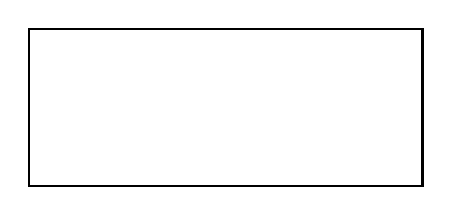
\begin{tikzpicture}
    \draw[thick] (0, 0) rectangle (5, 2);
\end{tikzpicture}
    \caption{The surface-mesh of the modelled dual-mode circular waveguide filter
    (left). An effort was made to keep the dimensions as similar to the ones
    given in \cite{DMCWF-Dimensions}, but a full correspondence cannot be guaranteed
    due to the author being unable to resolve certain ambiguities that were encountered.
    The model adheres to the following dimensions:
    $L_C=43.87$ mm, $D_C=28.0$ mm, $L_B=20.0$ mm, $W_B=19.05$ mm, $H_B=9.525$ mm,
    $W_S=10.05$ mm, $H_S=3.0$ mm, $W_A=2.0$ mm, $H_A=3.375$ mm,
    $L_A=2.825$ mm; The thickness of all irises is $2.0$ mm; The screws
    are placed exactly halfway up each of the two resonant cylinders,
    with the horizontal tuning screws reaching a depth of $3.82$ mm into the cavity
    and coupling screws at angles $\pm 45^{\circ}$ with a depth of $3.57$ mm.
    Observe that the \acrshort{DMCWF} is point symmetric with respect to the center 
    of the cross iris.}
    \label{fig:DMCWF}
\end{figure}

% Modeling process cite rubia
I created the model in the computer-aided design modeler software application
FreeCAD\footnote{\url{https://www.freecadweb.org/}}. The mesh was defined using 
the 3D finite element mesh generator Gmsh\footnote{\url{https://gmsh.info/}} and 
is available for download on the git repository 
of this project \cite{git}. In Gmsh, a element size factor of 0.2 and 5 smoothing steps
are used for the Delaunay 3D meshing algorithm. Additionally, 
the mesh was refined around critical components such as the screws and irises
using transfinite curves (the sharp-eyed reader may observe these refinements
in the surface mesh visualized in Figure \ref{fig:DMCWF}). A total of
185726 \acrshort{DOF}s are accounted for. The conversion of the
mesh to the FEniCS supported .xml format was performed with the open source mesh
format converter meshio\footnote{\url{https://github.com/nschloe/meshio}}. 

% Scattering coefficient
In the following, I would like to demonstrate the capability of the 
\acrshort{gMRI} algorithm to approximate scattering coefficients for the \acrshort{DMCWF}.
The definition of the scattering matrix is a adaptation from \cite{shortMRI} to
\begin{equation}
    \mathbf{\underline{S}}(\omega) = \mathbf{\underline{Id}}
    - 2\left( \mathbf{\underline{Id}} + i \frac{\omega}{2\pi} \sqrt{\frac{\mu}{\epsilon}}
    \sqrt{\frac{1 - (\omega_c / \omega_0)^2}{1 - (\omega_c / \omega)^2}} 
    \mathbf{\underline{F}}^H \mathbf{\underline{U}}(\omega) \right)^{-1}
\end{equation}
where $\mathbf{\underline{F}} = [\mathbf{f}_1, \mathbf{f}_2]$ and
$\mathbf{\underline{U}} = [\mathbf{u}_1, \mathbf{u}_2]$ with $\mathbf{f}_1$ the source term
resulting when the \acrshort{DMCWF} is forced from one side, producing the
solution $\mathbf{u}_1$, and the $\mathbf{f}_2$ when forcing from the other side to
produce $\mathbf{u}_2$. $\omega_c = 4.122 \times 10^{10}$ and $\omega_0 = 6.283 \times 10^{10}$
were assumed. The scattering coefficients $S_{ij}$ are then precisely the
entries of the scattering matrix
\begin{equation}
    \mathbf{\underline{S}}(\omega) =
    \begin{bmatrix}
            S_{11}(\omega) & S_{12}(\omega) \\
            S_{21}(\omega) & S_{22}(\omega)
    \end{bmatrix}\label{equ:scattering-coefficients}
\end{equation}

For the simulation, $\epsilon = 4 \pi \times 10^{-7}$ and 
$\mu = 8.854187 \times 10^{-12}$ were assumed. The one-sided forcing
was performed with $\left.\mathbf{g}\right|_{\Gamma_L} = - \mathbf{e}_z$ from the
left-hand inlet $\Gamma_L$, and $\left.\mathbf{g}\right|_{\Gamma_R} = \mathbf{e}_z$ from the
right-hand inlet $\Gamma_R$. The scattering coefficients $S_{11}(\omega)$ and $S_{21}(\omega)$
once computed by using the solutions at 150 uniformly spaced sample frequencies
directly obtained with the \acrshort{FEM},
and once from the rational surrogate computed with \acrshort{gMRI} at a tolerance
of $\tau = 10^{-2}$ and 1000 uniformly spaced candidate test points in
the frequency range $\omega \in [7.257 \times 10^{10}, 7.508 \times 10^{10}]$. Both are shown (but only one is seen) in Figure
\ref{fig:circular-waveguide-scattering}. At somewhat more than four minutes,
the \acrshort{gMRI} was able to deliver the approximated scattering coefficients
roughly 25 times faster than the \acrshort{FEM}. Compared to \cite{DMCWF-FrequencySweep},
the passband is similar in shape but slightly shifted towards the left, i.e. lower
frequencies.

\begin{figure}[ht]
    \centering
    %% Creator: Matplotlib, PGF backend
%%
%% To include the figure in your LaTeX document, write
%%   \input{<filename>.pgf}
%%
%% Make sure the required packages are loaded in your preamble
%%   \usepackage{pgf}
%%
%% Also ensure that all the required font packages are loaded; for instance,
%% the lmodern package is sometimes necessary when using math font.
%%   \usepackage{lmodern}
%%
%% Figures using additional raster images can only be included by \input if
%% they are in the same directory as the main LaTeX file. For loading figures
%% from other directories you can use the `import` package
%%   \usepackage{import}
%%
%% and then include the figures with
%%   \import{<path to file>}{<filename>.pgf}
%%
%% Matplotlib used the following preamble
%%   \usepackage{fontspec}
%%   \setmainfont{DejaVuSans.ttf}[Path=\detokenize{C:/Users/Fabio/Anaconda3/Lib/site-packages/matplotlib/mpl-data/fonts/ttf/}]
%%   \setsansfont{DejaVuSans.ttf}[Path=\detokenize{C:/Users/Fabio/Anaconda3/Lib/site-packages/matplotlib/mpl-data/fonts/ttf/}]
%%   \setmonofont{DejaVuSansMono.ttf}[Path=\detokenize{C:/Users/Fabio/Anaconda3/Lib/site-packages/matplotlib/mpl-data/fonts/ttf/}]
%%
\begingroup%
\makeatletter%
\begin{pgfpicture}%
\pgfpathrectangle{\pgfpointorigin}{\pgfqpoint{5.078495in}{2.551126in}}%
\pgfusepath{use as bounding box, clip}%
\begin{pgfscope}%
\pgfsetbuttcap%
\pgfsetmiterjoin%
\pgfsetlinewidth{0.000000pt}%
\definecolor{currentstroke}{rgb}{1.000000,1.000000,1.000000}%
\pgfsetstrokecolor{currentstroke}%
\pgfsetstrokeopacity{0.000000}%
\pgfsetdash{}{0pt}%
\pgfpathmoveto{\pgfqpoint{0.000000in}{0.000000in}}%
\pgfpathlineto{\pgfqpoint{5.078495in}{0.000000in}}%
\pgfpathlineto{\pgfqpoint{5.078495in}{2.551126in}}%
\pgfpathlineto{\pgfqpoint{0.000000in}{2.551126in}}%
\pgfpathlineto{\pgfqpoint{0.000000in}{0.000000in}}%
\pgfpathclose%
\pgfusepath{}%
\end{pgfscope}%
\begin{pgfscope}%
\pgfsetbuttcap%
\pgfsetmiterjoin%
\definecolor{currentfill}{rgb}{1.000000,1.000000,1.000000}%
\pgfsetfillcolor{currentfill}%
\pgfsetlinewidth{0.000000pt}%
\definecolor{currentstroke}{rgb}{0.000000,0.000000,0.000000}%
\pgfsetstrokecolor{currentstroke}%
\pgfsetstrokeopacity{0.000000}%
\pgfsetdash{}{0pt}%
\pgfpathmoveto{\pgfqpoint{0.677245in}{1.492236in}}%
\pgfpathlineto{\pgfqpoint{4.978495in}{1.492236in}}%
\pgfpathlineto{\pgfqpoint{4.978495in}{2.435986in}}%
\pgfpathlineto{\pgfqpoint{0.677245in}{2.435986in}}%
\pgfpathlineto{\pgfqpoint{0.677245in}{1.492236in}}%
\pgfpathclose%
\pgfusepath{fill}%
\end{pgfscope}%
\begin{pgfscope}%
\pgfsetbuttcap%
\pgfsetroundjoin%
\definecolor{currentfill}{rgb}{0.000000,0.000000,0.000000}%
\pgfsetfillcolor{currentfill}%
\pgfsetlinewidth{0.803000pt}%
\definecolor{currentstroke}{rgb}{0.000000,0.000000,0.000000}%
\pgfsetstrokecolor{currentstroke}%
\pgfsetdash{}{0pt}%
\pgfsys@defobject{currentmarker}{\pgfqpoint{0.000000in}{-0.048611in}}{\pgfqpoint{0.000000in}{0.000000in}}{%
\pgfpathmoveto{\pgfqpoint{0.000000in}{0.000000in}}%
\pgfpathlineto{\pgfqpoint{0.000000in}{-0.048611in}}%
\pgfusepath{stroke,fill}%
}%
\begin{pgfscope}%
\pgfsys@transformshift{1.411800in}{1.492236in}%
\pgfsys@useobject{currentmarker}{}%
\end{pgfscope}%
\end{pgfscope}%
\begin{pgfscope}%
\pgfsetbuttcap%
\pgfsetroundjoin%
\definecolor{currentfill}{rgb}{0.000000,0.000000,0.000000}%
\pgfsetfillcolor{currentfill}%
\pgfsetlinewidth{0.803000pt}%
\definecolor{currentstroke}{rgb}{0.000000,0.000000,0.000000}%
\pgfsetstrokecolor{currentstroke}%
\pgfsetdash{}{0pt}%
\pgfsys@defobject{currentmarker}{\pgfqpoint{0.000000in}{-0.048611in}}{\pgfqpoint{0.000000in}{0.000000in}}{%
\pgfpathmoveto{\pgfqpoint{0.000000in}{0.000000in}}%
\pgfpathlineto{\pgfqpoint{0.000000in}{-0.048611in}}%
\pgfusepath{stroke,fill}%
}%
\begin{pgfscope}%
\pgfsys@transformshift{2.267506in}{1.492236in}%
\pgfsys@useobject{currentmarker}{}%
\end{pgfscope}%
\end{pgfscope}%
\begin{pgfscope}%
\pgfsetbuttcap%
\pgfsetroundjoin%
\definecolor{currentfill}{rgb}{0.000000,0.000000,0.000000}%
\pgfsetfillcolor{currentfill}%
\pgfsetlinewidth{0.803000pt}%
\definecolor{currentstroke}{rgb}{0.000000,0.000000,0.000000}%
\pgfsetstrokecolor{currentstroke}%
\pgfsetdash{}{0pt}%
\pgfsys@defobject{currentmarker}{\pgfqpoint{0.000000in}{-0.048611in}}{\pgfqpoint{0.000000in}{0.000000in}}{%
\pgfpathmoveto{\pgfqpoint{0.000000in}{0.000000in}}%
\pgfpathlineto{\pgfqpoint{0.000000in}{-0.048611in}}%
\pgfusepath{stroke,fill}%
}%
\begin{pgfscope}%
\pgfsys@transformshift{3.123213in}{1.492236in}%
\pgfsys@useobject{currentmarker}{}%
\end{pgfscope}%
\end{pgfscope}%
\begin{pgfscope}%
\pgfsetbuttcap%
\pgfsetroundjoin%
\definecolor{currentfill}{rgb}{0.000000,0.000000,0.000000}%
\pgfsetfillcolor{currentfill}%
\pgfsetlinewidth{0.803000pt}%
\definecolor{currentstroke}{rgb}{0.000000,0.000000,0.000000}%
\pgfsetstrokecolor{currentstroke}%
\pgfsetdash{}{0pt}%
\pgfsys@defobject{currentmarker}{\pgfqpoint{0.000000in}{-0.048611in}}{\pgfqpoint{0.000000in}{0.000000in}}{%
\pgfpathmoveto{\pgfqpoint{0.000000in}{0.000000in}}%
\pgfpathlineto{\pgfqpoint{0.000000in}{-0.048611in}}%
\pgfusepath{stroke,fill}%
}%
\begin{pgfscope}%
\pgfsys@transformshift{3.978919in}{1.492236in}%
\pgfsys@useobject{currentmarker}{}%
\end{pgfscope}%
\end{pgfscope}%
\begin{pgfscope}%
\pgfsetbuttcap%
\pgfsetroundjoin%
\definecolor{currentfill}{rgb}{0.000000,0.000000,0.000000}%
\pgfsetfillcolor{currentfill}%
\pgfsetlinewidth{0.803000pt}%
\definecolor{currentstroke}{rgb}{0.000000,0.000000,0.000000}%
\pgfsetstrokecolor{currentstroke}%
\pgfsetdash{}{0pt}%
\pgfsys@defobject{currentmarker}{\pgfqpoint{0.000000in}{-0.048611in}}{\pgfqpoint{0.000000in}{0.000000in}}{%
\pgfpathmoveto{\pgfqpoint{0.000000in}{0.000000in}}%
\pgfpathlineto{\pgfqpoint{0.000000in}{-0.048611in}}%
\pgfusepath{stroke,fill}%
}%
\begin{pgfscope}%
\pgfsys@transformshift{4.834626in}{1.492236in}%
\pgfsys@useobject{currentmarker}{}%
\end{pgfscope}%
\end{pgfscope}%
\begin{pgfscope}%
\pgfpathrectangle{\pgfqpoint{0.677245in}{1.492236in}}{\pgfqpoint{4.301250in}{0.943750in}}%
\pgfusepath{clip}%
\pgfsetrectcap%
\pgfsetroundjoin%
\pgfsetlinewidth{0.803000pt}%
\definecolor{currentstroke}{rgb}{0.690196,0.690196,0.690196}%
\pgfsetstrokecolor{currentstroke}%
\pgfsetdash{}{0pt}%
\pgfpathmoveto{\pgfqpoint{0.677245in}{1.716142in}}%
\pgfpathlineto{\pgfqpoint{4.978495in}{1.716142in}}%
\pgfusepath{stroke}%
\end{pgfscope}%
\begin{pgfscope}%
\pgfsetbuttcap%
\pgfsetroundjoin%
\definecolor{currentfill}{rgb}{0.000000,0.000000,0.000000}%
\pgfsetfillcolor{currentfill}%
\pgfsetlinewidth{0.803000pt}%
\definecolor{currentstroke}{rgb}{0.000000,0.000000,0.000000}%
\pgfsetstrokecolor{currentstroke}%
\pgfsetdash{}{0pt}%
\pgfsys@defobject{currentmarker}{\pgfqpoint{-0.048611in}{0.000000in}}{\pgfqpoint{-0.000000in}{0.000000in}}{%
\pgfpathmoveto{\pgfqpoint{-0.000000in}{0.000000in}}%
\pgfpathlineto{\pgfqpoint{-0.048611in}{0.000000in}}%
\pgfusepath{stroke,fill}%
}%
\begin{pgfscope}%
\pgfsys@transformshift{0.677245in}{1.716142in}%
\pgfsys@useobject{currentmarker}{}%
\end{pgfscope}%
\end{pgfscope}%
\begin{pgfscope}%
\definecolor{textcolor}{rgb}{0.000000,0.000000,0.000000}%
\pgfsetstrokecolor{textcolor}%
\pgfsetfillcolor{textcolor}%
\pgftext[x=0.309652in, y=1.658105in, left, base]{\color{textcolor}\rmfamily\fontsize{11.000000}{13.200000}\selectfont \(\displaystyle {\ensuremath{-}40}\)}%
\end{pgfscope}%
\begin{pgfscope}%
\pgfpathrectangle{\pgfqpoint{0.677245in}{1.492236in}}{\pgfqpoint{4.301250in}{0.943750in}}%
\pgfusepath{clip}%
\pgfsetrectcap%
\pgfsetroundjoin%
\pgfsetlinewidth{0.803000pt}%
\definecolor{currentstroke}{rgb}{0.690196,0.690196,0.690196}%
\pgfsetstrokecolor{currentstroke}%
\pgfsetdash{}{0pt}%
\pgfpathmoveto{\pgfqpoint{0.677245in}{2.054615in}}%
\pgfpathlineto{\pgfqpoint{4.978495in}{2.054615in}}%
\pgfusepath{stroke}%
\end{pgfscope}%
\begin{pgfscope}%
\pgfsetbuttcap%
\pgfsetroundjoin%
\definecolor{currentfill}{rgb}{0.000000,0.000000,0.000000}%
\pgfsetfillcolor{currentfill}%
\pgfsetlinewidth{0.803000pt}%
\definecolor{currentstroke}{rgb}{0.000000,0.000000,0.000000}%
\pgfsetstrokecolor{currentstroke}%
\pgfsetdash{}{0pt}%
\pgfsys@defobject{currentmarker}{\pgfqpoint{-0.048611in}{0.000000in}}{\pgfqpoint{-0.000000in}{0.000000in}}{%
\pgfpathmoveto{\pgfqpoint{-0.000000in}{0.000000in}}%
\pgfpathlineto{\pgfqpoint{-0.048611in}{0.000000in}}%
\pgfusepath{stroke,fill}%
}%
\begin{pgfscope}%
\pgfsys@transformshift{0.677245in}{2.054615in}%
\pgfsys@useobject{currentmarker}{}%
\end{pgfscope}%
\end{pgfscope}%
\begin{pgfscope}%
\definecolor{textcolor}{rgb}{0.000000,0.000000,0.000000}%
\pgfsetstrokecolor{textcolor}%
\pgfsetfillcolor{textcolor}%
\pgftext[x=0.309652in, y=1.996578in, left, base]{\color{textcolor}\rmfamily\fontsize{11.000000}{13.200000}\selectfont \(\displaystyle {\ensuremath{-}20}\)}%
\end{pgfscope}%
\begin{pgfscope}%
\pgfpathrectangle{\pgfqpoint{0.677245in}{1.492236in}}{\pgfqpoint{4.301250in}{0.943750in}}%
\pgfusepath{clip}%
\pgfsetrectcap%
\pgfsetroundjoin%
\pgfsetlinewidth{0.803000pt}%
\definecolor{currentstroke}{rgb}{0.690196,0.690196,0.690196}%
\pgfsetstrokecolor{currentstroke}%
\pgfsetdash{}{0pt}%
\pgfpathmoveto{\pgfqpoint{0.677245in}{2.393088in}}%
\pgfpathlineto{\pgfqpoint{4.978495in}{2.393088in}}%
\pgfusepath{stroke}%
\end{pgfscope}%
\begin{pgfscope}%
\pgfsetbuttcap%
\pgfsetroundjoin%
\definecolor{currentfill}{rgb}{0.000000,0.000000,0.000000}%
\pgfsetfillcolor{currentfill}%
\pgfsetlinewidth{0.803000pt}%
\definecolor{currentstroke}{rgb}{0.000000,0.000000,0.000000}%
\pgfsetstrokecolor{currentstroke}%
\pgfsetdash{}{0pt}%
\pgfsys@defobject{currentmarker}{\pgfqpoint{-0.048611in}{0.000000in}}{\pgfqpoint{-0.000000in}{0.000000in}}{%
\pgfpathmoveto{\pgfqpoint{-0.000000in}{0.000000in}}%
\pgfpathlineto{\pgfqpoint{-0.048611in}{0.000000in}}%
\pgfusepath{stroke,fill}%
}%
\begin{pgfscope}%
\pgfsys@transformshift{0.677245in}{2.393088in}%
\pgfsys@useobject{currentmarker}{}%
\end{pgfscope}%
\end{pgfscope}%
\begin{pgfscope}%
\definecolor{textcolor}{rgb}{0.000000,0.000000,0.000000}%
\pgfsetstrokecolor{textcolor}%
\pgfsetfillcolor{textcolor}%
\pgftext[x=0.503981in, y=2.335050in, left, base]{\color{textcolor}\rmfamily\fontsize{11.000000}{13.200000}\selectfont \(\displaystyle {0}\)}%
\end{pgfscope}%
\begin{pgfscope}%
\definecolor{textcolor}{rgb}{0.000000,0.000000,0.000000}%
\pgfsetstrokecolor{textcolor}%
\pgfsetfillcolor{textcolor}%
\pgftext[x=0.254096in,y=1.964111in,,bottom,rotate=90.000000]{\color{textcolor}\rmfamily\fontsize{11.000000}{13.200000}\selectfont \(\displaystyle S_{11}(\omega)\) (dB)}%
\end{pgfscope}%
\begin{pgfscope}%
\pgfpathrectangle{\pgfqpoint{0.677245in}{1.492236in}}{\pgfqpoint{4.301250in}{0.943750in}}%
\pgfusepath{clip}%
\pgfsetrectcap%
\pgfsetroundjoin%
\pgfsetlinewidth{1.505625pt}%
\definecolor{currentstroke}{rgb}{0.001462,0.000466,0.013866}%
\pgfsetstrokecolor{currentstroke}%
\pgfsetdash{}{0pt}%
\pgfpathmoveto{\pgfqpoint{0.677245in}{2.392326in}}%
\pgfpathlineto{\pgfqpoint{1.831943in}{2.391587in}}%
\pgfpathlineto{\pgfqpoint{2.005147in}{2.392742in}}%
\pgfpathlineto{\pgfqpoint{2.062882in}{2.389398in}}%
\pgfpathlineto{\pgfqpoint{2.091750in}{2.385044in}}%
\pgfpathlineto{\pgfqpoint{2.120617in}{2.377238in}}%
\pgfpathlineto{\pgfqpoint{2.149485in}{2.363722in}}%
\pgfpathlineto{\pgfqpoint{2.178352in}{2.340971in}}%
\pgfpathlineto{\pgfqpoint{2.207219in}{2.303723in}}%
\pgfpathlineto{\pgfqpoint{2.236087in}{2.244847in}}%
\pgfpathlineto{\pgfqpoint{2.264954in}{2.155038in}}%
\pgfpathlineto{\pgfqpoint{2.293822in}{2.020826in}}%
\pgfpathlineto{\pgfqpoint{2.322689in}{1.814862in}}%
\pgfpathlineto{\pgfqpoint{2.351557in}{1.535134in}}%
\pgfpathlineto{\pgfqpoint{2.380424in}{1.676903in}}%
\pgfpathlineto{\pgfqpoint{2.409292in}{1.853100in}}%
\pgfpathlineto{\pgfqpoint{2.438159in}{1.954282in}}%
\pgfpathlineto{\pgfqpoint{2.467026in}{2.018252in}}%
\pgfpathlineto{\pgfqpoint{2.495894in}{2.061510in}}%
\pgfpathlineto{\pgfqpoint{2.524761in}{2.092187in}}%
\pgfpathlineto{\pgfqpoint{2.553629in}{2.114399in}}%
\pgfpathlineto{\pgfqpoint{2.582496in}{2.130779in}}%
\pgfpathlineto{\pgfqpoint{2.611364in}{2.142717in}}%
\pgfpathlineto{\pgfqpoint{2.640231in}{2.151317in}}%
\pgfpathlineto{\pgfqpoint{2.669099in}{2.157074in}}%
\pgfpathlineto{\pgfqpoint{2.697966in}{2.160504in}}%
\pgfpathlineto{\pgfqpoint{2.726834in}{2.161706in}}%
\pgfpathlineto{\pgfqpoint{2.755701in}{2.160889in}}%
\pgfpathlineto{\pgfqpoint{2.784568in}{2.157905in}}%
\pgfpathlineto{\pgfqpoint{2.813436in}{2.152720in}}%
\pgfpathlineto{\pgfqpoint{2.842303in}{2.144930in}}%
\pgfpathlineto{\pgfqpoint{2.871171in}{2.134186in}}%
\pgfpathlineto{\pgfqpoint{2.900038in}{2.119670in}}%
\pgfpathlineto{\pgfqpoint{2.928906in}{2.100436in}}%
\pgfpathlineto{\pgfqpoint{2.957773in}{2.074762in}}%
\pgfpathlineto{\pgfqpoint{2.986641in}{2.040254in}}%
\pgfpathlineto{\pgfqpoint{3.015508in}{1.992768in}}%
\pgfpathlineto{\pgfqpoint{3.044375in}{1.925791in}}%
\pgfpathlineto{\pgfqpoint{3.073243in}{1.829545in}}%
\pgfpathlineto{\pgfqpoint{3.102110in}{1.709749in}}%
\pgfpathlineto{\pgfqpoint{3.130978in}{1.707962in}}%
\pgfpathlineto{\pgfqpoint{3.159845in}{1.871353in}}%
\pgfpathlineto{\pgfqpoint{3.188713in}{2.022153in}}%
\pgfpathlineto{\pgfqpoint{3.217580in}{2.134281in}}%
\pgfpathlineto{\pgfqpoint{3.246448in}{2.215680in}}%
\pgfpathlineto{\pgfqpoint{3.275315in}{2.273769in}}%
\pgfpathlineto{\pgfqpoint{3.304183in}{2.314248in}}%
\pgfpathlineto{\pgfqpoint{3.333050in}{2.341876in}}%
\pgfpathlineto{\pgfqpoint{3.361917in}{2.360385in}}%
\pgfpathlineto{\pgfqpoint{3.390785in}{2.372634in}}%
\pgfpathlineto{\pgfqpoint{3.419652in}{2.380639in}}%
\pgfpathlineto{\pgfqpoint{3.448520in}{2.385807in}}%
\pgfpathlineto{\pgfqpoint{3.506255in}{2.391086in}}%
\pgfpathlineto{\pgfqpoint{3.592857in}{2.393085in}}%
\pgfpathlineto{\pgfqpoint{3.766062in}{2.391571in}}%
\pgfpathlineto{\pgfqpoint{4.141339in}{2.388107in}}%
\pgfpathlineto{\pgfqpoint{4.632085in}{2.387190in}}%
\pgfpathlineto{\pgfqpoint{4.978495in}{2.387580in}}%
\pgfpathlineto{\pgfqpoint{4.978495in}{2.387580in}}%
\pgfusepath{stroke}%
\end{pgfscope}%
\begin{pgfscope}%
\pgfpathrectangle{\pgfqpoint{0.677245in}{1.492236in}}{\pgfqpoint{4.301250in}{0.943750in}}%
\pgfusepath{clip}%
\pgfsetrectcap%
\pgfsetroundjoin%
\pgfsetlinewidth{1.505625pt}%
\definecolor{currentstroke}{rgb}{0.735683,0.215906,0.330245}%
\pgfsetstrokecolor{currentstroke}%
\pgfsetdash{}{0pt}%
\pgfpathmoveto{\pgfqpoint{0.677245in}{2.392326in}}%
\pgfpathlineto{\pgfqpoint{1.831943in}{2.391587in}}%
\pgfpathlineto{\pgfqpoint{2.005147in}{2.392742in}}%
\pgfpathlineto{\pgfqpoint{2.062882in}{2.389398in}}%
\pgfpathlineto{\pgfqpoint{2.091750in}{2.385044in}}%
\pgfpathlineto{\pgfqpoint{2.120617in}{2.377238in}}%
\pgfpathlineto{\pgfqpoint{2.149485in}{2.363722in}}%
\pgfpathlineto{\pgfqpoint{2.178352in}{2.340971in}}%
\pgfpathlineto{\pgfqpoint{2.207219in}{2.303723in}}%
\pgfpathlineto{\pgfqpoint{2.236087in}{2.244847in}}%
\pgfpathlineto{\pgfqpoint{2.264954in}{2.155038in}}%
\pgfpathlineto{\pgfqpoint{2.293822in}{2.020825in}}%
\pgfpathlineto{\pgfqpoint{2.322689in}{1.814860in}}%
\pgfpathlineto{\pgfqpoint{2.351557in}{1.535134in}}%
\pgfpathlineto{\pgfqpoint{2.380424in}{1.676907in}}%
\pgfpathlineto{\pgfqpoint{2.409292in}{1.853102in}}%
\pgfpathlineto{\pgfqpoint{2.438159in}{1.954283in}}%
\pgfpathlineto{\pgfqpoint{2.467026in}{2.018253in}}%
\pgfpathlineto{\pgfqpoint{2.495894in}{2.061511in}}%
\pgfpathlineto{\pgfqpoint{2.524761in}{2.092187in}}%
\pgfpathlineto{\pgfqpoint{2.553629in}{2.114399in}}%
\pgfpathlineto{\pgfqpoint{2.582496in}{2.130780in}}%
\pgfpathlineto{\pgfqpoint{2.611364in}{2.142717in}}%
\pgfpathlineto{\pgfqpoint{2.640231in}{2.151318in}}%
\pgfpathlineto{\pgfqpoint{2.669099in}{2.157075in}}%
\pgfpathlineto{\pgfqpoint{2.697966in}{2.160504in}}%
\pgfpathlineto{\pgfqpoint{2.726834in}{2.161706in}}%
\pgfpathlineto{\pgfqpoint{2.755701in}{2.160890in}}%
\pgfpathlineto{\pgfqpoint{2.784568in}{2.157905in}}%
\pgfpathlineto{\pgfqpoint{2.813436in}{2.152721in}}%
\pgfpathlineto{\pgfqpoint{2.842303in}{2.144930in}}%
\pgfpathlineto{\pgfqpoint{2.871171in}{2.134187in}}%
\pgfpathlineto{\pgfqpoint{2.900038in}{2.119670in}}%
\pgfpathlineto{\pgfqpoint{2.928906in}{2.100436in}}%
\pgfpathlineto{\pgfqpoint{2.957773in}{2.074762in}}%
\pgfpathlineto{\pgfqpoint{2.986641in}{2.040254in}}%
\pgfpathlineto{\pgfqpoint{3.015508in}{1.992768in}}%
\pgfpathlineto{\pgfqpoint{3.044375in}{1.925792in}}%
\pgfpathlineto{\pgfqpoint{3.073243in}{1.829545in}}%
\pgfpathlineto{\pgfqpoint{3.102110in}{1.709749in}}%
\pgfpathlineto{\pgfqpoint{3.130978in}{1.707961in}}%
\pgfpathlineto{\pgfqpoint{3.159845in}{1.871353in}}%
\pgfpathlineto{\pgfqpoint{3.188713in}{2.022153in}}%
\pgfpathlineto{\pgfqpoint{3.217580in}{2.134281in}}%
\pgfpathlineto{\pgfqpoint{3.246448in}{2.215680in}}%
\pgfpathlineto{\pgfqpoint{3.275315in}{2.273769in}}%
\pgfpathlineto{\pgfqpoint{3.304183in}{2.314248in}}%
\pgfpathlineto{\pgfqpoint{3.333050in}{2.341876in}}%
\pgfpathlineto{\pgfqpoint{3.361917in}{2.360385in}}%
\pgfpathlineto{\pgfqpoint{3.390785in}{2.372634in}}%
\pgfpathlineto{\pgfqpoint{3.419652in}{2.380639in}}%
\pgfpathlineto{\pgfqpoint{3.448520in}{2.385807in}}%
\pgfpathlineto{\pgfqpoint{3.506255in}{2.391086in}}%
\pgfpathlineto{\pgfqpoint{3.592857in}{2.393085in}}%
\pgfpathlineto{\pgfqpoint{3.766062in}{2.391571in}}%
\pgfpathlineto{\pgfqpoint{4.141339in}{2.388106in}}%
\pgfpathlineto{\pgfqpoint{4.632085in}{2.387189in}}%
\pgfpathlineto{\pgfqpoint{4.978495in}{2.387580in}}%
\pgfpathlineto{\pgfqpoint{4.978495in}{2.387580in}}%
\pgfusepath{stroke}%
\end{pgfscope}%
\begin{pgfscope}%
\pgfsetrectcap%
\pgfsetmiterjoin%
\pgfsetlinewidth{0.803000pt}%
\definecolor{currentstroke}{rgb}{0.000000,0.000000,0.000000}%
\pgfsetstrokecolor{currentstroke}%
\pgfsetdash{}{0pt}%
\pgfpathmoveto{\pgfqpoint{0.677245in}{1.492236in}}%
\pgfpathlineto{\pgfqpoint{0.677245in}{2.435986in}}%
\pgfusepath{stroke}%
\end{pgfscope}%
\begin{pgfscope}%
\pgfsetrectcap%
\pgfsetmiterjoin%
\pgfsetlinewidth{0.803000pt}%
\definecolor{currentstroke}{rgb}{0.000000,0.000000,0.000000}%
\pgfsetstrokecolor{currentstroke}%
\pgfsetdash{}{0pt}%
\pgfpathmoveto{\pgfqpoint{4.978495in}{1.492236in}}%
\pgfpathlineto{\pgfqpoint{4.978495in}{2.435986in}}%
\pgfusepath{stroke}%
\end{pgfscope}%
\begin{pgfscope}%
\pgfsetrectcap%
\pgfsetmiterjoin%
\pgfsetlinewidth{0.803000pt}%
\definecolor{currentstroke}{rgb}{0.000000,0.000000,0.000000}%
\pgfsetstrokecolor{currentstroke}%
\pgfsetdash{}{0pt}%
\pgfpathmoveto{\pgfqpoint{0.677245in}{1.492236in}}%
\pgfpathlineto{\pgfqpoint{4.978495in}{1.492236in}}%
\pgfusepath{stroke}%
\end{pgfscope}%
\begin{pgfscope}%
\pgfsetrectcap%
\pgfsetmiterjoin%
\pgfsetlinewidth{0.803000pt}%
\definecolor{currentstroke}{rgb}{0.000000,0.000000,0.000000}%
\pgfsetstrokecolor{currentstroke}%
\pgfsetdash{}{0pt}%
\pgfpathmoveto{\pgfqpoint{0.677245in}{2.435986in}}%
\pgfpathlineto{\pgfqpoint{4.978495in}{2.435986in}}%
\pgfusepath{stroke}%
\end{pgfscope}%
\begin{pgfscope}%
\pgfsetbuttcap%
\pgfsetmiterjoin%
\definecolor{currentfill}{rgb}{1.000000,1.000000,1.000000}%
\pgfsetfillcolor{currentfill}%
\pgfsetfillopacity{0.800000}%
\pgfsetlinewidth{1.003750pt}%
\definecolor{currentstroke}{rgb}{0.800000,0.800000,0.800000}%
\pgfsetstrokecolor{currentstroke}%
\pgfsetstrokeopacity{0.800000}%
\pgfsetdash{}{0pt}%
\pgfpathmoveto{\pgfqpoint{3.653162in}{1.568625in}}%
\pgfpathlineto{\pgfqpoint{4.871550in}{1.568625in}}%
\pgfpathquadraticcurveto{\pgfqpoint{4.902106in}{1.568625in}}{\pgfqpoint{4.902106in}{1.599180in}}%
\pgfpathlineto{\pgfqpoint{4.902106in}{2.032388in}}%
\pgfpathquadraticcurveto{\pgfqpoint{4.902106in}{2.062944in}}{\pgfqpoint{4.871550in}{2.062944in}}%
\pgfpathlineto{\pgfqpoint{3.653162in}{2.062944in}}%
\pgfpathquadraticcurveto{\pgfqpoint{3.622607in}{2.062944in}}{\pgfqpoint{3.622607in}{2.032388in}}%
\pgfpathlineto{\pgfqpoint{3.622607in}{1.599180in}}%
\pgfpathquadraticcurveto{\pgfqpoint{3.622607in}{1.568625in}}{\pgfqpoint{3.653162in}{1.568625in}}%
\pgfpathlineto{\pgfqpoint{3.653162in}{1.568625in}}%
\pgfpathclose%
\pgfusepath{stroke,fill}%
\end{pgfscope}%
\begin{pgfscope}%
\pgfsetrectcap%
\pgfsetroundjoin%
\pgfsetlinewidth{1.505625pt}%
\definecolor{currentstroke}{rgb}{0.001462,0.000466,0.013866}%
\pgfsetstrokecolor{currentstroke}%
\pgfsetdash{}{0pt}%
\pgfpathmoveto{\pgfqpoint{3.683718in}{1.939230in}}%
\pgfpathlineto{\pgfqpoint{3.836496in}{1.939230in}}%
\pgfpathlineto{\pgfqpoint{3.989273in}{1.939230in}}%
\pgfusepath{stroke}%
\end{pgfscope}%
\begin{pgfscope}%
\definecolor{textcolor}{rgb}{0.000000,0.000000,0.000000}%
\pgfsetstrokecolor{textcolor}%
\pgfsetfillcolor{textcolor}%
\pgftext[x=4.111496in,y=1.885757in,left,base]{\color{textcolor}\rmfamily\fontsize{11.000000}{13.200000}\selectfont reference}%
\end{pgfscope}%
\begin{pgfscope}%
\pgfsetrectcap%
\pgfsetroundjoin%
\pgfsetlinewidth{1.505625pt}%
\definecolor{currentstroke}{rgb}{0.735683,0.215906,0.330245}%
\pgfsetstrokecolor{currentstroke}%
\pgfsetdash{}{0pt}%
\pgfpathmoveto{\pgfqpoint{3.683718in}{1.714987in}}%
\pgfpathlineto{\pgfqpoint{3.836496in}{1.714987in}}%
\pgfpathlineto{\pgfqpoint{3.989273in}{1.714987in}}%
\pgfusepath{stroke}%
\end{pgfscope}%
\begin{pgfscope}%
\definecolor{textcolor}{rgb}{0.000000,0.000000,0.000000}%
\pgfsetstrokecolor{textcolor}%
\pgfsetfillcolor{textcolor}%
\pgftext[x=4.111496in,y=1.661515in,left,base]{\color{textcolor}\rmfamily\fontsize{11.000000}{13.200000}\selectfont gMRI}%
\end{pgfscope}%
\begin{pgfscope}%
\pgfsetbuttcap%
\pgfsetmiterjoin%
\definecolor{currentfill}{rgb}{1.000000,1.000000,1.000000}%
\pgfsetfillcolor{currentfill}%
\pgfsetlinewidth{0.000000pt}%
\definecolor{currentstroke}{rgb}{0.000000,0.000000,0.000000}%
\pgfsetstrokecolor{currentstroke}%
\pgfsetstrokeopacity{0.000000}%
\pgfsetdash{}{0pt}%
\pgfpathmoveto{\pgfqpoint{0.677245in}{0.548486in}}%
\pgfpathlineto{\pgfqpoint{4.978495in}{0.548486in}}%
\pgfpathlineto{\pgfqpoint{4.978495in}{1.492236in}}%
\pgfpathlineto{\pgfqpoint{0.677245in}{1.492236in}}%
\pgfpathlineto{\pgfqpoint{0.677245in}{0.548486in}}%
\pgfpathclose%
\pgfusepath{fill}%
\end{pgfscope}%
\begin{pgfscope}%
\pgfsetbuttcap%
\pgfsetroundjoin%
\definecolor{currentfill}{rgb}{0.000000,0.000000,0.000000}%
\pgfsetfillcolor{currentfill}%
\pgfsetlinewidth{0.803000pt}%
\definecolor{currentstroke}{rgb}{0.000000,0.000000,0.000000}%
\pgfsetstrokecolor{currentstroke}%
\pgfsetdash{}{0pt}%
\pgfsys@defobject{currentmarker}{\pgfqpoint{0.000000in}{-0.048611in}}{\pgfqpoint{0.000000in}{0.000000in}}{%
\pgfpathmoveto{\pgfqpoint{0.000000in}{0.000000in}}%
\pgfpathlineto{\pgfqpoint{0.000000in}{-0.048611in}}%
\pgfusepath{stroke,fill}%
}%
\begin{pgfscope}%
\pgfsys@transformshift{1.411800in}{0.548486in}%
\pgfsys@useobject{currentmarker}{}%
\end{pgfscope}%
\end{pgfscope}%
\begin{pgfscope}%
\definecolor{textcolor}{rgb}{0.000000,0.000000,0.000000}%
\pgfsetstrokecolor{textcolor}%
\pgfsetfillcolor{textcolor}%
\pgftext[x=1.411800in,y=0.451264in,,top]{\color{textcolor}\rmfamily\fontsize{11.000000}{13.200000}\selectfont \(\displaystyle {7.30}\)}%
\end{pgfscope}%
\begin{pgfscope}%
\pgfsetbuttcap%
\pgfsetroundjoin%
\definecolor{currentfill}{rgb}{0.000000,0.000000,0.000000}%
\pgfsetfillcolor{currentfill}%
\pgfsetlinewidth{0.803000pt}%
\definecolor{currentstroke}{rgb}{0.000000,0.000000,0.000000}%
\pgfsetstrokecolor{currentstroke}%
\pgfsetdash{}{0pt}%
\pgfsys@defobject{currentmarker}{\pgfqpoint{0.000000in}{-0.048611in}}{\pgfqpoint{0.000000in}{0.000000in}}{%
\pgfpathmoveto{\pgfqpoint{0.000000in}{0.000000in}}%
\pgfpathlineto{\pgfqpoint{0.000000in}{-0.048611in}}%
\pgfusepath{stroke,fill}%
}%
\begin{pgfscope}%
\pgfsys@transformshift{2.267506in}{0.548486in}%
\pgfsys@useobject{currentmarker}{}%
\end{pgfscope}%
\end{pgfscope}%
\begin{pgfscope}%
\definecolor{textcolor}{rgb}{0.000000,0.000000,0.000000}%
\pgfsetstrokecolor{textcolor}%
\pgfsetfillcolor{textcolor}%
\pgftext[x=2.267506in,y=0.451264in,,top]{\color{textcolor}\rmfamily\fontsize{11.000000}{13.200000}\selectfont \(\displaystyle {7.35}\)}%
\end{pgfscope}%
\begin{pgfscope}%
\pgfsetbuttcap%
\pgfsetroundjoin%
\definecolor{currentfill}{rgb}{0.000000,0.000000,0.000000}%
\pgfsetfillcolor{currentfill}%
\pgfsetlinewidth{0.803000pt}%
\definecolor{currentstroke}{rgb}{0.000000,0.000000,0.000000}%
\pgfsetstrokecolor{currentstroke}%
\pgfsetdash{}{0pt}%
\pgfsys@defobject{currentmarker}{\pgfqpoint{0.000000in}{-0.048611in}}{\pgfqpoint{0.000000in}{0.000000in}}{%
\pgfpathmoveto{\pgfqpoint{0.000000in}{0.000000in}}%
\pgfpathlineto{\pgfqpoint{0.000000in}{-0.048611in}}%
\pgfusepath{stroke,fill}%
}%
\begin{pgfscope}%
\pgfsys@transformshift{3.123213in}{0.548486in}%
\pgfsys@useobject{currentmarker}{}%
\end{pgfscope}%
\end{pgfscope}%
\begin{pgfscope}%
\definecolor{textcolor}{rgb}{0.000000,0.000000,0.000000}%
\pgfsetstrokecolor{textcolor}%
\pgfsetfillcolor{textcolor}%
\pgftext[x=3.123213in,y=0.451264in,,top]{\color{textcolor}\rmfamily\fontsize{11.000000}{13.200000}\selectfont \(\displaystyle {7.40}\)}%
\end{pgfscope}%
\begin{pgfscope}%
\pgfsetbuttcap%
\pgfsetroundjoin%
\definecolor{currentfill}{rgb}{0.000000,0.000000,0.000000}%
\pgfsetfillcolor{currentfill}%
\pgfsetlinewidth{0.803000pt}%
\definecolor{currentstroke}{rgb}{0.000000,0.000000,0.000000}%
\pgfsetstrokecolor{currentstroke}%
\pgfsetdash{}{0pt}%
\pgfsys@defobject{currentmarker}{\pgfqpoint{0.000000in}{-0.048611in}}{\pgfqpoint{0.000000in}{0.000000in}}{%
\pgfpathmoveto{\pgfqpoint{0.000000in}{0.000000in}}%
\pgfpathlineto{\pgfqpoint{0.000000in}{-0.048611in}}%
\pgfusepath{stroke,fill}%
}%
\begin{pgfscope}%
\pgfsys@transformshift{3.978919in}{0.548486in}%
\pgfsys@useobject{currentmarker}{}%
\end{pgfscope}%
\end{pgfscope}%
\begin{pgfscope}%
\definecolor{textcolor}{rgb}{0.000000,0.000000,0.000000}%
\pgfsetstrokecolor{textcolor}%
\pgfsetfillcolor{textcolor}%
\pgftext[x=3.978919in,y=0.451264in,,top]{\color{textcolor}\rmfamily\fontsize{11.000000}{13.200000}\selectfont \(\displaystyle {7.45}\)}%
\end{pgfscope}%
\begin{pgfscope}%
\pgfsetbuttcap%
\pgfsetroundjoin%
\definecolor{currentfill}{rgb}{0.000000,0.000000,0.000000}%
\pgfsetfillcolor{currentfill}%
\pgfsetlinewidth{0.803000pt}%
\definecolor{currentstroke}{rgb}{0.000000,0.000000,0.000000}%
\pgfsetstrokecolor{currentstroke}%
\pgfsetdash{}{0pt}%
\pgfsys@defobject{currentmarker}{\pgfqpoint{0.000000in}{-0.048611in}}{\pgfqpoint{0.000000in}{0.000000in}}{%
\pgfpathmoveto{\pgfqpoint{0.000000in}{0.000000in}}%
\pgfpathlineto{\pgfqpoint{0.000000in}{-0.048611in}}%
\pgfusepath{stroke,fill}%
}%
\begin{pgfscope}%
\pgfsys@transformshift{4.834626in}{0.548486in}%
\pgfsys@useobject{currentmarker}{}%
\end{pgfscope}%
\end{pgfscope}%
\begin{pgfscope}%
\definecolor{textcolor}{rgb}{0.000000,0.000000,0.000000}%
\pgfsetstrokecolor{textcolor}%
\pgfsetfillcolor{textcolor}%
\pgftext[x=4.834626in,y=0.451264in,,top]{\color{textcolor}\rmfamily\fontsize{11.000000}{13.200000}\selectfont \(\displaystyle {7.50}\)}%
\end{pgfscope}%
\begin{pgfscope}%
\definecolor{textcolor}{rgb}{0.000000,0.000000,0.000000}%
\pgfsetstrokecolor{textcolor}%
\pgfsetfillcolor{textcolor}%
\pgftext[x=2.827870in,y=0.247854in,,top]{\color{textcolor}\rmfamily\fontsize{11.000000}{13.200000}\selectfont Frequency \(\displaystyle \omega\)}%
\end{pgfscope}%
\begin{pgfscope}%
\definecolor{textcolor}{rgb}{0.000000,0.000000,0.000000}%
\pgfsetstrokecolor{textcolor}%
\pgfsetfillcolor{textcolor}%
\pgftext[x=4.978495in,y=0.261743in,right,top]{\color{textcolor}\rmfamily\fontsize{11.000000}{13.200000}\selectfont \(\displaystyle \times{10^{10}}{}\)}%
\end{pgfscope}%
\begin{pgfscope}%
\pgfpathrectangle{\pgfqpoint{0.677245in}{0.548486in}}{\pgfqpoint{4.301250in}{0.943750in}}%
\pgfusepath{clip}%
\pgfsetrectcap%
\pgfsetroundjoin%
\pgfsetlinewidth{0.803000pt}%
\definecolor{currentstroke}{rgb}{0.690196,0.690196,0.690196}%
\pgfsetstrokecolor{currentstroke}%
\pgfsetdash{}{0pt}%
\pgfpathmoveto{\pgfqpoint{0.677245in}{0.990150in}}%
\pgfpathlineto{\pgfqpoint{4.978495in}{0.990150in}}%
\pgfusepath{stroke}%
\end{pgfscope}%
\begin{pgfscope}%
\pgfsetbuttcap%
\pgfsetroundjoin%
\definecolor{currentfill}{rgb}{0.000000,0.000000,0.000000}%
\pgfsetfillcolor{currentfill}%
\pgfsetlinewidth{0.803000pt}%
\definecolor{currentstroke}{rgb}{0.000000,0.000000,0.000000}%
\pgfsetstrokecolor{currentstroke}%
\pgfsetdash{}{0pt}%
\pgfsys@defobject{currentmarker}{\pgfqpoint{-0.048611in}{0.000000in}}{\pgfqpoint{-0.000000in}{0.000000in}}{%
\pgfpathmoveto{\pgfqpoint{-0.000000in}{0.000000in}}%
\pgfpathlineto{\pgfqpoint{-0.048611in}{0.000000in}}%
\pgfusepath{stroke,fill}%
}%
\begin{pgfscope}%
\pgfsys@transformshift{0.677245in}{0.990150in}%
\pgfsys@useobject{currentmarker}{}%
\end{pgfscope}%
\end{pgfscope}%
\begin{pgfscope}%
\definecolor{textcolor}{rgb}{0.000000,0.000000,0.000000}%
\pgfsetstrokecolor{textcolor}%
\pgfsetfillcolor{textcolor}%
\pgftext[x=0.309652in, y=0.932112in, left, base]{\color{textcolor}\rmfamily\fontsize{11.000000}{13.200000}\selectfont \(\displaystyle {\ensuremath{-}50}\)}%
\end{pgfscope}%
\begin{pgfscope}%
\pgfpathrectangle{\pgfqpoint{0.677245in}{0.548486in}}{\pgfqpoint{4.301250in}{0.943750in}}%
\pgfusepath{clip}%
\pgfsetrectcap%
\pgfsetroundjoin%
\pgfsetlinewidth{0.803000pt}%
\definecolor{currentstroke}{rgb}{0.690196,0.690196,0.690196}%
\pgfsetstrokecolor{currentstroke}%
\pgfsetdash{}{0pt}%
\pgfpathmoveto{\pgfqpoint{0.677245in}{1.449338in}}%
\pgfpathlineto{\pgfqpoint{4.978495in}{1.449338in}}%
\pgfusepath{stroke}%
\end{pgfscope}%
\begin{pgfscope}%
\pgfsetbuttcap%
\pgfsetroundjoin%
\definecolor{currentfill}{rgb}{0.000000,0.000000,0.000000}%
\pgfsetfillcolor{currentfill}%
\pgfsetlinewidth{0.803000pt}%
\definecolor{currentstroke}{rgb}{0.000000,0.000000,0.000000}%
\pgfsetstrokecolor{currentstroke}%
\pgfsetdash{}{0pt}%
\pgfsys@defobject{currentmarker}{\pgfqpoint{-0.048611in}{0.000000in}}{\pgfqpoint{-0.000000in}{0.000000in}}{%
\pgfpathmoveto{\pgfqpoint{-0.000000in}{0.000000in}}%
\pgfpathlineto{\pgfqpoint{-0.048611in}{0.000000in}}%
\pgfusepath{stroke,fill}%
}%
\begin{pgfscope}%
\pgfsys@transformshift{0.677245in}{1.449338in}%
\pgfsys@useobject{currentmarker}{}%
\end{pgfscope}%
\end{pgfscope}%
\begin{pgfscope}%
\definecolor{textcolor}{rgb}{0.000000,0.000000,0.000000}%
\pgfsetstrokecolor{textcolor}%
\pgfsetfillcolor{textcolor}%
\pgftext[x=0.503981in, y=1.391300in, left, base]{\color{textcolor}\rmfamily\fontsize{11.000000}{13.200000}\selectfont \(\displaystyle {0}\)}%
\end{pgfscope}%
\begin{pgfscope}%
\definecolor{textcolor}{rgb}{0.000000,0.000000,0.000000}%
\pgfsetstrokecolor{textcolor}%
\pgfsetfillcolor{textcolor}%
\pgftext[x=0.254096in,y=1.020361in,,bottom,rotate=90.000000]{\color{textcolor}\rmfamily\fontsize{11.000000}{13.200000}\selectfont \(\displaystyle S_{12}(\omega)\) (dB)}%
\end{pgfscope}%
\begin{pgfscope}%
\pgfpathrectangle{\pgfqpoint{0.677245in}{0.548486in}}{\pgfqpoint{4.301250in}{0.943750in}}%
\pgfusepath{clip}%
\pgfsetrectcap%
\pgfsetroundjoin%
\pgfsetlinewidth{1.505625pt}%
\definecolor{currentstroke}{rgb}{0.001462,0.000466,0.013866}%
\pgfsetstrokecolor{currentstroke}%
\pgfsetdash{}{0pt}%
\pgfpathmoveto{\pgfqpoint{0.677245in}{0.955280in}}%
\pgfpathlineto{\pgfqpoint{0.994787in}{1.015047in}}%
\pgfpathlineto{\pgfqpoint{1.167991in}{1.044437in}}%
\pgfpathlineto{\pgfqpoint{1.283461in}{1.061399in}}%
\pgfpathlineto{\pgfqpoint{1.370063in}{1.071948in}}%
\pgfpathlineto{\pgfqpoint{1.456666in}{1.079773in}}%
\pgfpathlineto{\pgfqpoint{1.514401in}{1.082900in}}%
\pgfpathlineto{\pgfqpoint{1.572136in}{1.083729in}}%
\pgfpathlineto{\pgfqpoint{1.629870in}{1.081426in}}%
\pgfpathlineto{\pgfqpoint{1.687605in}{1.074652in}}%
\pgfpathlineto{\pgfqpoint{1.716473in}{1.068920in}}%
\pgfpathlineto{\pgfqpoint{1.745340in}{1.061078in}}%
\pgfpathlineto{\pgfqpoint{1.774208in}{1.050464in}}%
\pgfpathlineto{\pgfqpoint{1.803075in}{1.036124in}}%
\pgfpathlineto{\pgfqpoint{1.831943in}{1.016485in}}%
\pgfpathlineto{\pgfqpoint{1.860810in}{0.988866in}}%
\pgfpathlineto{\pgfqpoint{1.889677in}{0.947912in}}%
\pgfpathlineto{\pgfqpoint{1.918545in}{0.880677in}}%
\pgfpathlineto{\pgfqpoint{1.976280in}{0.591384in}}%
\pgfpathlineto{\pgfqpoint{2.005147in}{0.884946in}}%
\pgfpathlineto{\pgfqpoint{2.034015in}{1.010537in}}%
\pgfpathlineto{\pgfqpoint{2.062882in}{1.097951in}}%
\pgfpathlineto{\pgfqpoint{2.091750in}{1.168137in}}%
\pgfpathlineto{\pgfqpoint{2.120617in}{1.228250in}}%
\pgfpathlineto{\pgfqpoint{2.149485in}{1.281257in}}%
\pgfpathlineto{\pgfqpoint{2.178352in}{1.327994in}}%
\pgfpathlineto{\pgfqpoint{2.207219in}{1.368102in}}%
\pgfpathlineto{\pgfqpoint{2.236087in}{1.400453in}}%
\pgfpathlineto{\pgfqpoint{2.264954in}{1.424113in}}%
\pgfpathlineto{\pgfqpoint{2.293822in}{1.439129in}}%
\pgfpathlineto{\pgfqpoint{2.322689in}{1.446853in}}%
\pgfpathlineto{\pgfqpoint{2.351557in}{1.449338in}}%
\pgfpathlineto{\pgfqpoint{2.380424in}{1.448573in}}%
\pgfpathlineto{\pgfqpoint{2.438159in}{1.442777in}}%
\pgfpathlineto{\pgfqpoint{2.553629in}{1.430263in}}%
\pgfpathlineto{\pgfqpoint{2.640231in}{1.424759in}}%
\pgfpathlineto{\pgfqpoint{2.726834in}{1.422908in}}%
\pgfpathlineto{\pgfqpoint{2.813436in}{1.424518in}}%
\pgfpathlineto{\pgfqpoint{2.900038in}{1.429567in}}%
\pgfpathlineto{\pgfqpoint{2.986641in}{1.437726in}}%
\pgfpathlineto{\pgfqpoint{3.073243in}{1.446570in}}%
\pgfpathlineto{\pgfqpoint{3.102110in}{1.448283in}}%
\pgfpathlineto{\pgfqpoint{3.130978in}{1.448300in}}%
\pgfpathlineto{\pgfqpoint{3.159845in}{1.445609in}}%
\pgfpathlineto{\pgfqpoint{3.188713in}{1.439039in}}%
\pgfpathlineto{\pgfqpoint{3.217580in}{1.427489in}}%
\pgfpathlineto{\pgfqpoint{3.246448in}{1.410283in}}%
\pgfpathlineto{\pgfqpoint{3.275315in}{1.387347in}}%
\pgfpathlineto{\pgfqpoint{3.304183in}{1.359215in}}%
\pgfpathlineto{\pgfqpoint{3.333050in}{1.326619in}}%
\pgfpathlineto{\pgfqpoint{3.361917in}{1.290259in}}%
\pgfpathlineto{\pgfqpoint{3.390785in}{1.250422in}}%
\pgfpathlineto{\pgfqpoint{3.419652in}{1.207002in}}%
\pgfpathlineto{\pgfqpoint{3.448520in}{1.159206in}}%
\pgfpathlineto{\pgfqpoint{3.477387in}{1.105457in}}%
\pgfpathlineto{\pgfqpoint{3.506255in}{1.042541in}}%
\pgfpathlineto{\pgfqpoint{3.535122in}{0.963750in}}%
\pgfpathlineto{\pgfqpoint{3.563990in}{0.850937in}}%
\pgfpathlineto{\pgfqpoint{3.592857in}{0.611056in}}%
\pgfpathlineto{\pgfqpoint{3.621724in}{0.662489in}}%
\pgfpathlineto{\pgfqpoint{3.650592in}{0.832377in}}%
\pgfpathlineto{\pgfqpoint{3.679459in}{0.909882in}}%
\pgfpathlineto{\pgfqpoint{3.708327in}{0.958168in}}%
\pgfpathlineto{\pgfqpoint{3.737194in}{0.992041in}}%
\pgfpathlineto{\pgfqpoint{3.766062in}{1.017407in}}%
\pgfpathlineto{\pgfqpoint{3.794929in}{1.037179in}}%
\pgfpathlineto{\pgfqpoint{3.823797in}{1.053046in}}%
\pgfpathlineto{\pgfqpoint{3.852664in}{1.066032in}}%
\pgfpathlineto{\pgfqpoint{3.881531in}{1.076838in}}%
\pgfpathlineto{\pgfqpoint{3.939266in}{1.093660in}}%
\pgfpathlineto{\pgfqpoint{3.997001in}{1.105982in}}%
\pgfpathlineto{\pgfqpoint{4.054736in}{1.115208in}}%
\pgfpathlineto{\pgfqpoint{4.141339in}{1.125058in}}%
\pgfpathlineto{\pgfqpoint{4.227941in}{1.131608in}}%
\pgfpathlineto{\pgfqpoint{4.343411in}{1.136932in}}%
\pgfpathlineto{\pgfqpoint{4.487748in}{1.139958in}}%
\pgfpathlineto{\pgfqpoint{4.660953in}{1.140103in}}%
\pgfpathlineto{\pgfqpoint{4.863025in}{1.137037in}}%
\pgfpathlineto{\pgfqpoint{4.978495in}{1.134116in}}%
\pgfpathlineto{\pgfqpoint{4.978495in}{1.134116in}}%
\pgfusepath{stroke}%
\end{pgfscope}%
\begin{pgfscope}%
\pgfpathrectangle{\pgfqpoint{0.677245in}{0.548486in}}{\pgfqpoint{4.301250in}{0.943750in}}%
\pgfusepath{clip}%
\pgfsetrectcap%
\pgfsetroundjoin%
\pgfsetlinewidth{1.505625pt}%
\definecolor{currentstroke}{rgb}{0.735683,0.215906,0.330245}%
\pgfsetstrokecolor{currentstroke}%
\pgfsetdash{}{0pt}%
\pgfpathmoveto{\pgfqpoint{0.677245in}{0.955280in}}%
\pgfpathlineto{\pgfqpoint{0.965919in}{1.009862in}}%
\pgfpathlineto{\pgfqpoint{1.139124in}{1.039827in}}%
\pgfpathlineto{\pgfqpoint{1.283461in}{1.061407in}}%
\pgfpathlineto{\pgfqpoint{1.370063in}{1.071955in}}%
\pgfpathlineto{\pgfqpoint{1.456666in}{1.079778in}}%
\pgfpathlineto{\pgfqpoint{1.514401in}{1.082904in}}%
\pgfpathlineto{\pgfqpoint{1.572136in}{1.083733in}}%
\pgfpathlineto{\pgfqpoint{1.629870in}{1.081428in}}%
\pgfpathlineto{\pgfqpoint{1.687605in}{1.074654in}}%
\pgfpathlineto{\pgfqpoint{1.716473in}{1.068922in}}%
\pgfpathlineto{\pgfqpoint{1.745340in}{1.061079in}}%
\pgfpathlineto{\pgfqpoint{1.774208in}{1.050465in}}%
\pgfpathlineto{\pgfqpoint{1.803075in}{1.036125in}}%
\pgfpathlineto{\pgfqpoint{1.831943in}{1.016485in}}%
\pgfpathlineto{\pgfqpoint{1.860810in}{0.988867in}}%
\pgfpathlineto{\pgfqpoint{1.889677in}{0.947913in}}%
\pgfpathlineto{\pgfqpoint{1.918545in}{0.880678in}}%
\pgfpathlineto{\pgfqpoint{1.976280in}{0.591384in}}%
\pgfpathlineto{\pgfqpoint{2.005147in}{0.884946in}}%
\pgfpathlineto{\pgfqpoint{2.034015in}{1.010537in}}%
\pgfpathlineto{\pgfqpoint{2.062882in}{1.097951in}}%
\pgfpathlineto{\pgfqpoint{2.091750in}{1.168137in}}%
\pgfpathlineto{\pgfqpoint{2.120617in}{1.228250in}}%
\pgfpathlineto{\pgfqpoint{2.149485in}{1.281257in}}%
\pgfpathlineto{\pgfqpoint{2.178352in}{1.327994in}}%
\pgfpathlineto{\pgfqpoint{2.207219in}{1.368101in}}%
\pgfpathlineto{\pgfqpoint{2.236087in}{1.400454in}}%
\pgfpathlineto{\pgfqpoint{2.264954in}{1.424113in}}%
\pgfpathlineto{\pgfqpoint{2.293822in}{1.439129in}}%
\pgfpathlineto{\pgfqpoint{2.322689in}{1.446853in}}%
\pgfpathlineto{\pgfqpoint{2.351557in}{1.449338in}}%
\pgfpathlineto{\pgfqpoint{2.380424in}{1.448573in}}%
\pgfpathlineto{\pgfqpoint{2.438159in}{1.442777in}}%
\pgfpathlineto{\pgfqpoint{2.553629in}{1.430263in}}%
\pgfpathlineto{\pgfqpoint{2.640231in}{1.424759in}}%
\pgfpathlineto{\pgfqpoint{2.726834in}{1.422908in}}%
\pgfpathlineto{\pgfqpoint{2.813436in}{1.424518in}}%
\pgfpathlineto{\pgfqpoint{2.900038in}{1.429567in}}%
\pgfpathlineto{\pgfqpoint{2.986641in}{1.437726in}}%
\pgfpathlineto{\pgfqpoint{3.073243in}{1.446570in}}%
\pgfpathlineto{\pgfqpoint{3.102110in}{1.448283in}}%
\pgfpathlineto{\pgfqpoint{3.130978in}{1.448300in}}%
\pgfpathlineto{\pgfqpoint{3.159845in}{1.445609in}}%
\pgfpathlineto{\pgfqpoint{3.188713in}{1.439039in}}%
\pgfpathlineto{\pgfqpoint{3.217580in}{1.427489in}}%
\pgfpathlineto{\pgfqpoint{3.246448in}{1.410283in}}%
\pgfpathlineto{\pgfqpoint{3.275315in}{1.387347in}}%
\pgfpathlineto{\pgfqpoint{3.304183in}{1.359215in}}%
\pgfpathlineto{\pgfqpoint{3.333050in}{1.326619in}}%
\pgfpathlineto{\pgfqpoint{3.361917in}{1.290259in}}%
\pgfpathlineto{\pgfqpoint{3.390785in}{1.250422in}}%
\pgfpathlineto{\pgfqpoint{3.419652in}{1.207012in}}%
\pgfpathlineto{\pgfqpoint{3.448520in}{1.159204in}}%
\pgfpathlineto{\pgfqpoint{3.477387in}{1.105454in}}%
\pgfpathlineto{\pgfqpoint{3.506255in}{1.042535in}}%
\pgfpathlineto{\pgfqpoint{3.535122in}{0.963740in}}%
\pgfpathlineto{\pgfqpoint{3.563990in}{0.850916in}}%
\pgfpathlineto{\pgfqpoint{3.592857in}{0.610966in}}%
\pgfpathlineto{\pgfqpoint{3.621724in}{0.662568in}}%
\pgfpathlineto{\pgfqpoint{3.650592in}{0.832413in}}%
\pgfpathlineto{\pgfqpoint{3.679459in}{0.909909in}}%
\pgfpathlineto{\pgfqpoint{3.708327in}{0.958192in}}%
\pgfpathlineto{\pgfqpoint{3.737194in}{0.992063in}}%
\pgfpathlineto{\pgfqpoint{3.766062in}{1.017428in}}%
\pgfpathlineto{\pgfqpoint{3.794929in}{1.037200in}}%
\pgfpathlineto{\pgfqpoint{3.823797in}{1.053068in}}%
\pgfpathlineto{\pgfqpoint{3.852664in}{1.066055in}}%
\pgfpathlineto{\pgfqpoint{3.881531in}{1.076861in}}%
\pgfpathlineto{\pgfqpoint{3.939266in}{1.093685in}}%
\pgfpathlineto{\pgfqpoint{3.997001in}{1.106008in}}%
\pgfpathlineto{\pgfqpoint{4.054736in}{1.115237in}}%
\pgfpathlineto{\pgfqpoint{4.141339in}{1.125090in}}%
\pgfpathlineto{\pgfqpoint{4.227941in}{1.131644in}}%
\pgfpathlineto{\pgfqpoint{4.343411in}{1.136971in}}%
\pgfpathlineto{\pgfqpoint{4.487748in}{1.140000in}}%
\pgfpathlineto{\pgfqpoint{4.660953in}{1.140143in}}%
\pgfpathlineto{\pgfqpoint{4.863025in}{1.137059in}}%
\pgfpathlineto{\pgfqpoint{4.978495in}{1.134116in}}%
\pgfpathlineto{\pgfqpoint{4.978495in}{1.134116in}}%
\pgfusepath{stroke}%
\end{pgfscope}%
\begin{pgfscope}%
\pgfsetrectcap%
\pgfsetmiterjoin%
\pgfsetlinewidth{0.803000pt}%
\definecolor{currentstroke}{rgb}{0.000000,0.000000,0.000000}%
\pgfsetstrokecolor{currentstroke}%
\pgfsetdash{}{0pt}%
\pgfpathmoveto{\pgfqpoint{0.677245in}{0.548486in}}%
\pgfpathlineto{\pgfqpoint{0.677245in}{1.492236in}}%
\pgfusepath{stroke}%
\end{pgfscope}%
\begin{pgfscope}%
\pgfsetrectcap%
\pgfsetmiterjoin%
\pgfsetlinewidth{0.803000pt}%
\definecolor{currentstroke}{rgb}{0.000000,0.000000,0.000000}%
\pgfsetstrokecolor{currentstroke}%
\pgfsetdash{}{0pt}%
\pgfpathmoveto{\pgfqpoint{4.978495in}{0.548486in}}%
\pgfpathlineto{\pgfqpoint{4.978495in}{1.492236in}}%
\pgfusepath{stroke}%
\end{pgfscope}%
\begin{pgfscope}%
\pgfsetrectcap%
\pgfsetmiterjoin%
\pgfsetlinewidth{0.803000pt}%
\definecolor{currentstroke}{rgb}{0.000000,0.000000,0.000000}%
\pgfsetstrokecolor{currentstroke}%
\pgfsetdash{}{0pt}%
\pgfpathmoveto{\pgfqpoint{0.677245in}{0.548486in}}%
\pgfpathlineto{\pgfqpoint{4.978495in}{0.548486in}}%
\pgfusepath{stroke}%
\end{pgfscope}%
\begin{pgfscope}%
\pgfsetrectcap%
\pgfsetmiterjoin%
\pgfsetlinewidth{0.803000pt}%
\definecolor{currentstroke}{rgb}{0.000000,0.000000,0.000000}%
\pgfsetstrokecolor{currentstroke}%
\pgfsetdash{}{0pt}%
\pgfpathmoveto{\pgfqpoint{0.677245in}{1.492236in}}%
\pgfpathlineto{\pgfqpoint{4.978495in}{1.492236in}}%
\pgfusepath{stroke}%
\end{pgfscope}%
\end{pgfpicture}%
\makeatother%
\endgroup%

    \caption{The scattering coefficients $S_{11}(\omega)$ and $S_{21}(\omega)$
    defined in (\ref{equ:scattering-coefficients}) computed as a reference
    from solving the system at discrete sample points and the
    \acrshort{FEM}, as well as the ones obtained by using \acrshort{gMRI}.}
    \label{fig:circular-waveguide-scattering}
\end{figure}

The progression of the
absolute error with the number of support points used to build the surrogate
can be seen in Figure \ref{fig:circular-waveguide-error}.

\begin{figure}[ht]
    \centering
    %% Creator: Matplotlib, PGF backend
%%
%% To include the figure in your LaTeX document, write
%%   \input{<filename>.pgf}
%%
%% Make sure the required packages are loaded in your preamble
%%   \usepackage{pgf}
%%
%% Also ensure that all the required font packages are loaded; for instance,
%% the lmodern package is sometimes necessary when using math font.
%%   \usepackage{lmodern}
%%
%% Figures using additional raster images can only be included by \input if
%% they are in the same directory as the main LaTeX file. For loading figures
%% from other directories you can use the `import` package
%%   \usepackage{import}
%%
%% and then include the figures with
%%   \import{<path to file>}{<filename>.pgf}
%%
%% Matplotlib used the following preamble
%%   \usepackage{fontspec}
%%   \setmainfont{DejaVuSans.ttf}[Path=\detokenize{C:/Users/Fabio/Anaconda3/Lib/site-packages/matplotlib/mpl-data/fonts/ttf/}]
%%   \setsansfont{DejaVuSans.ttf}[Path=\detokenize{C:/Users/Fabio/Anaconda3/Lib/site-packages/matplotlib/mpl-data/fonts/ttf/}]
%%   \setmonofont{DejaVuSansMono.ttf}[Path=\detokenize{C:/Users/Fabio/Anaconda3/Lib/site-packages/matplotlib/mpl-data/fonts/ttf/}]
%%
\begingroup%
\makeatletter%
\begin{pgfpicture}%
\pgfpathrectangle{\pgfpointorigin}{\pgfqpoint{5.371152in}{4.149370in}}%
\pgfusepath{use as bounding box, clip}%
\begin{pgfscope}%
\pgfsetbuttcap%
\pgfsetmiterjoin%
\pgfsetlinewidth{0.000000pt}%
\definecolor{currentstroke}{rgb}{1.000000,1.000000,1.000000}%
\pgfsetstrokecolor{currentstroke}%
\pgfsetstrokeopacity{0.000000}%
\pgfsetdash{}{0pt}%
\pgfpathmoveto{\pgfqpoint{0.000000in}{0.000000in}}%
\pgfpathlineto{\pgfqpoint{5.371152in}{0.000000in}}%
\pgfpathlineto{\pgfqpoint{5.371152in}{4.149370in}}%
\pgfpathlineto{\pgfqpoint{0.000000in}{4.149370in}}%
\pgfpathlineto{\pgfqpoint{0.000000in}{0.000000in}}%
\pgfpathclose%
\pgfusepath{}%
\end{pgfscope}%
\begin{pgfscope}%
\pgfsetbuttcap%
\pgfsetmiterjoin%
\definecolor{currentfill}{rgb}{1.000000,1.000000,1.000000}%
\pgfsetfillcolor{currentfill}%
\pgfsetlinewidth{0.000000pt}%
\definecolor{currentstroke}{rgb}{0.000000,0.000000,0.000000}%
\pgfsetstrokecolor{currentstroke}%
\pgfsetstrokeopacity{0.000000}%
\pgfsetdash{}{0pt}%
\pgfpathmoveto{\pgfqpoint{0.767489in}{2.247236in}}%
\pgfpathlineto{\pgfqpoint{5.068739in}{2.247236in}}%
\pgfpathlineto{\pgfqpoint{5.068739in}{3.945986in}}%
\pgfpathlineto{\pgfqpoint{0.767489in}{3.945986in}}%
\pgfpathlineto{\pgfqpoint{0.767489in}{2.247236in}}%
\pgfpathclose%
\pgfusepath{fill}%
\end{pgfscope}%
\begin{pgfscope}%
\pgfsetbuttcap%
\pgfsetroundjoin%
\definecolor{currentfill}{rgb}{0.000000,0.000000,0.000000}%
\pgfsetfillcolor{currentfill}%
\pgfsetlinewidth{0.803000pt}%
\definecolor{currentstroke}{rgb}{0.000000,0.000000,0.000000}%
\pgfsetstrokecolor{currentstroke}%
\pgfsetdash{}{0pt}%
\pgfsys@defobject{currentmarker}{\pgfqpoint{0.000000in}{-0.048611in}}{\pgfqpoint{0.000000in}{0.000000in}}{%
\pgfpathmoveto{\pgfqpoint{0.000000in}{0.000000in}}%
\pgfpathlineto{\pgfqpoint{0.000000in}{-0.048611in}}%
\pgfusepath{stroke,fill}%
}%
\begin{pgfscope}%
\pgfsys@transformshift{1.482778in}{2.247236in}%
\pgfsys@useobject{currentmarker}{}%
\end{pgfscope}%
\end{pgfscope}%
\begin{pgfscope}%
\pgfsetbuttcap%
\pgfsetroundjoin%
\definecolor{currentfill}{rgb}{0.000000,0.000000,0.000000}%
\pgfsetfillcolor{currentfill}%
\pgfsetlinewidth{0.803000pt}%
\definecolor{currentstroke}{rgb}{0.000000,0.000000,0.000000}%
\pgfsetstrokecolor{currentstroke}%
\pgfsetdash{}{0pt}%
\pgfsys@defobject{currentmarker}{\pgfqpoint{0.000000in}{-0.048611in}}{\pgfqpoint{0.000000in}{0.000000in}}{%
\pgfpathmoveto{\pgfqpoint{0.000000in}{0.000000in}}%
\pgfpathlineto{\pgfqpoint{0.000000in}{-0.048611in}}%
\pgfusepath{stroke,fill}%
}%
\begin{pgfscope}%
\pgfsys@transformshift{2.350127in}{2.247236in}%
\pgfsys@useobject{currentmarker}{}%
\end{pgfscope}%
\end{pgfscope}%
\begin{pgfscope}%
\pgfsetbuttcap%
\pgfsetroundjoin%
\definecolor{currentfill}{rgb}{0.000000,0.000000,0.000000}%
\pgfsetfillcolor{currentfill}%
\pgfsetlinewidth{0.803000pt}%
\definecolor{currentstroke}{rgb}{0.000000,0.000000,0.000000}%
\pgfsetstrokecolor{currentstroke}%
\pgfsetdash{}{0pt}%
\pgfsys@defobject{currentmarker}{\pgfqpoint{0.000000in}{-0.048611in}}{\pgfqpoint{0.000000in}{0.000000in}}{%
\pgfpathmoveto{\pgfqpoint{0.000000in}{0.000000in}}%
\pgfpathlineto{\pgfqpoint{0.000000in}{-0.048611in}}%
\pgfusepath{stroke,fill}%
}%
\begin{pgfscope}%
\pgfsys@transformshift{3.217476in}{2.247236in}%
\pgfsys@useobject{currentmarker}{}%
\end{pgfscope}%
\end{pgfscope}%
\begin{pgfscope}%
\pgfsetbuttcap%
\pgfsetroundjoin%
\definecolor{currentfill}{rgb}{0.000000,0.000000,0.000000}%
\pgfsetfillcolor{currentfill}%
\pgfsetlinewidth{0.803000pt}%
\definecolor{currentstroke}{rgb}{0.000000,0.000000,0.000000}%
\pgfsetstrokecolor{currentstroke}%
\pgfsetdash{}{0pt}%
\pgfsys@defobject{currentmarker}{\pgfqpoint{0.000000in}{-0.048611in}}{\pgfqpoint{0.000000in}{0.000000in}}{%
\pgfpathmoveto{\pgfqpoint{0.000000in}{0.000000in}}%
\pgfpathlineto{\pgfqpoint{0.000000in}{-0.048611in}}%
\pgfusepath{stroke,fill}%
}%
\begin{pgfscope}%
\pgfsys@transformshift{4.084825in}{2.247236in}%
\pgfsys@useobject{currentmarker}{}%
\end{pgfscope}%
\end{pgfscope}%
\begin{pgfscope}%
\pgfsetbuttcap%
\pgfsetroundjoin%
\definecolor{currentfill}{rgb}{0.000000,0.000000,0.000000}%
\pgfsetfillcolor{currentfill}%
\pgfsetlinewidth{0.803000pt}%
\definecolor{currentstroke}{rgb}{0.000000,0.000000,0.000000}%
\pgfsetstrokecolor{currentstroke}%
\pgfsetdash{}{0pt}%
\pgfsys@defobject{currentmarker}{\pgfqpoint{0.000000in}{-0.048611in}}{\pgfqpoint{0.000000in}{0.000000in}}{%
\pgfpathmoveto{\pgfqpoint{0.000000in}{0.000000in}}%
\pgfpathlineto{\pgfqpoint{0.000000in}{-0.048611in}}%
\pgfusepath{stroke,fill}%
}%
\begin{pgfscope}%
\pgfsys@transformshift{4.952173in}{2.247236in}%
\pgfsys@useobject{currentmarker}{}%
\end{pgfscope}%
\end{pgfscope}%
\begin{pgfscope}%
\pgfpathrectangle{\pgfqpoint{0.767489in}{2.247236in}}{\pgfqpoint{4.301250in}{1.698750in}}%
\pgfusepath{clip}%
\pgfsetrectcap%
\pgfsetroundjoin%
\pgfsetlinewidth{0.803000pt}%
\definecolor{currentstroke}{rgb}{0.690196,0.690196,0.690196}%
\pgfsetstrokecolor{currentstroke}%
\pgfsetdash{}{0pt}%
\pgfpathmoveto{\pgfqpoint{0.767489in}{2.629515in}}%
\pgfpathlineto{\pgfqpoint{5.068739in}{2.629515in}}%
\pgfusepath{stroke}%
\end{pgfscope}%
\begin{pgfscope}%
\pgfsetbuttcap%
\pgfsetroundjoin%
\definecolor{currentfill}{rgb}{0.000000,0.000000,0.000000}%
\pgfsetfillcolor{currentfill}%
\pgfsetlinewidth{0.803000pt}%
\definecolor{currentstroke}{rgb}{0.000000,0.000000,0.000000}%
\pgfsetstrokecolor{currentstroke}%
\pgfsetdash{}{0pt}%
\pgfsys@defobject{currentmarker}{\pgfqpoint{-0.048611in}{0.000000in}}{\pgfqpoint{-0.000000in}{0.000000in}}{%
\pgfpathmoveto{\pgfqpoint{-0.000000in}{0.000000in}}%
\pgfpathlineto{\pgfqpoint{-0.048611in}{0.000000in}}%
\pgfusepath{stroke,fill}%
}%
\begin{pgfscope}%
\pgfsys@transformshift{0.767489in}{2.629515in}%
\pgfsys@useobject{currentmarker}{}%
\end{pgfscope}%
\end{pgfscope}%
\begin{pgfscope}%
\definecolor{textcolor}{rgb}{0.000000,0.000000,0.000000}%
\pgfsetstrokecolor{textcolor}%
\pgfsetfillcolor{textcolor}%
\pgftext[x=0.360388in, y=2.571477in, left, base]{\color{textcolor}\rmfamily\fontsize{11.000000}{13.200000}\selectfont \(\displaystyle {10^{-8}}\)}%
\end{pgfscope}%
\begin{pgfscope}%
\pgfpathrectangle{\pgfqpoint{0.767489in}{2.247236in}}{\pgfqpoint{4.301250in}{1.698750in}}%
\pgfusepath{clip}%
\pgfsetrectcap%
\pgfsetroundjoin%
\pgfsetlinewidth{0.803000pt}%
\definecolor{currentstroke}{rgb}{0.690196,0.690196,0.690196}%
\pgfsetstrokecolor{currentstroke}%
\pgfsetdash{}{0pt}%
\pgfpathmoveto{\pgfqpoint{0.767489in}{3.096339in}}%
\pgfpathlineto{\pgfqpoint{5.068739in}{3.096339in}}%
\pgfusepath{stroke}%
\end{pgfscope}%
\begin{pgfscope}%
\pgfsetbuttcap%
\pgfsetroundjoin%
\definecolor{currentfill}{rgb}{0.000000,0.000000,0.000000}%
\pgfsetfillcolor{currentfill}%
\pgfsetlinewidth{0.803000pt}%
\definecolor{currentstroke}{rgb}{0.000000,0.000000,0.000000}%
\pgfsetstrokecolor{currentstroke}%
\pgfsetdash{}{0pt}%
\pgfsys@defobject{currentmarker}{\pgfqpoint{-0.048611in}{0.000000in}}{\pgfqpoint{-0.000000in}{0.000000in}}{%
\pgfpathmoveto{\pgfqpoint{-0.000000in}{0.000000in}}%
\pgfpathlineto{\pgfqpoint{-0.048611in}{0.000000in}}%
\pgfusepath{stroke,fill}%
}%
\begin{pgfscope}%
\pgfsys@transformshift{0.767489in}{3.096339in}%
\pgfsys@useobject{currentmarker}{}%
\end{pgfscope}%
\end{pgfscope}%
\begin{pgfscope}%
\definecolor{textcolor}{rgb}{0.000000,0.000000,0.000000}%
\pgfsetstrokecolor{textcolor}%
\pgfsetfillcolor{textcolor}%
\pgftext[x=0.360388in, y=3.038301in, left, base]{\color{textcolor}\rmfamily\fontsize{11.000000}{13.200000}\selectfont \(\displaystyle {10^{-5}}\)}%
\end{pgfscope}%
\begin{pgfscope}%
\pgfpathrectangle{\pgfqpoint{0.767489in}{2.247236in}}{\pgfqpoint{4.301250in}{1.698750in}}%
\pgfusepath{clip}%
\pgfsetrectcap%
\pgfsetroundjoin%
\pgfsetlinewidth{0.803000pt}%
\definecolor{currentstroke}{rgb}{0.690196,0.690196,0.690196}%
\pgfsetstrokecolor{currentstroke}%
\pgfsetdash{}{0pt}%
\pgfpathmoveto{\pgfqpoint{0.767489in}{3.563164in}}%
\pgfpathlineto{\pgfqpoint{5.068739in}{3.563164in}}%
\pgfusepath{stroke}%
\end{pgfscope}%
\begin{pgfscope}%
\pgfsetbuttcap%
\pgfsetroundjoin%
\definecolor{currentfill}{rgb}{0.000000,0.000000,0.000000}%
\pgfsetfillcolor{currentfill}%
\pgfsetlinewidth{0.803000pt}%
\definecolor{currentstroke}{rgb}{0.000000,0.000000,0.000000}%
\pgfsetstrokecolor{currentstroke}%
\pgfsetdash{}{0pt}%
\pgfsys@defobject{currentmarker}{\pgfqpoint{-0.048611in}{0.000000in}}{\pgfqpoint{-0.000000in}{0.000000in}}{%
\pgfpathmoveto{\pgfqpoint{-0.000000in}{0.000000in}}%
\pgfpathlineto{\pgfqpoint{-0.048611in}{0.000000in}}%
\pgfusepath{stroke,fill}%
}%
\begin{pgfscope}%
\pgfsys@transformshift{0.767489in}{3.563164in}%
\pgfsys@useobject{currentmarker}{}%
\end{pgfscope}%
\end{pgfscope}%
\begin{pgfscope}%
\definecolor{textcolor}{rgb}{0.000000,0.000000,0.000000}%
\pgfsetstrokecolor{textcolor}%
\pgfsetfillcolor{textcolor}%
\pgftext[x=0.360388in, y=3.505126in, left, base]{\color{textcolor}\rmfamily\fontsize{11.000000}{13.200000}\selectfont \(\displaystyle {10^{-2}}\)}%
\end{pgfscope}%
\begin{pgfscope}%
\definecolor{textcolor}{rgb}{0.000000,0.000000,0.000000}%
\pgfsetstrokecolor{textcolor}%
\pgfsetfillcolor{textcolor}%
\pgftext[x=0.304833in,y=3.096611in,,bottom,rotate=90.000000]{\color{textcolor}\rmfamily\fontsize{11.000000}{13.200000}\selectfont \(\displaystyle |S_{11, \textrm{gMRI}}(\omega) - S_{11, \textrm{FEM}}(\omega)|\)}%
\end{pgfscope}%
\begin{pgfscope}%
\pgfpathrectangle{\pgfqpoint{0.767489in}{2.247236in}}{\pgfqpoint{4.301250in}{1.698750in}}%
\pgfusepath{clip}%
\pgfsetrectcap%
\pgfsetroundjoin%
\pgfsetlinewidth{1.505625pt}%
\definecolor{currentstroke}{rgb}{0.001462,0.000466,0.013866}%
\pgfsetstrokecolor{currentstroke}%
\pgfsetdash{}{0pt}%
\pgfpathmoveto{\pgfqpoint{0.767489in}{3.293701in}}%
\pgfpathlineto{\pgfqpoint{0.796750in}{3.342198in}}%
\pgfpathlineto{\pgfqpoint{0.826010in}{3.371245in}}%
\pgfpathlineto{\pgfqpoint{0.855270in}{3.392347in}}%
\pgfpathlineto{\pgfqpoint{0.884530in}{3.409074in}}%
\pgfpathlineto{\pgfqpoint{0.913790in}{3.423051in}}%
\pgfpathlineto{\pgfqpoint{0.972311in}{3.445768in}}%
\pgfpathlineto{\pgfqpoint{1.030831in}{3.464066in}}%
\pgfpathlineto{\pgfqpoint{1.089352in}{3.479510in}}%
\pgfpathlineto{\pgfqpoint{1.177132in}{3.498991in}}%
\pgfpathlineto{\pgfqpoint{1.264913in}{3.515207in}}%
\pgfpathlineto{\pgfqpoint{1.352694in}{3.528718in}}%
\pgfpathlineto{\pgfqpoint{1.440474in}{3.539653in}}%
\pgfpathlineto{\pgfqpoint{1.528255in}{3.547742in}}%
\pgfpathlineto{\pgfqpoint{1.616035in}{3.552285in}}%
\pgfpathlineto{\pgfqpoint{1.674556in}{3.552676in}}%
\pgfpathlineto{\pgfqpoint{1.733076in}{3.550121in}}%
\pgfpathlineto{\pgfqpoint{1.791597in}{3.543332in}}%
\pgfpathlineto{\pgfqpoint{1.820857in}{3.537674in}}%
\pgfpathlineto{\pgfqpoint{1.850117in}{3.529894in}}%
\pgfpathlineto{\pgfqpoint{1.879377in}{3.519264in}}%
\pgfpathlineto{\pgfqpoint{1.908637in}{3.504559in}}%
\pgfpathlineto{\pgfqpoint{1.937898in}{3.483660in}}%
\pgfpathlineto{\pgfqpoint{1.967158in}{3.452181in}}%
\pgfpathlineto{\pgfqpoint{1.996418in}{3.398632in}}%
\pgfpathlineto{\pgfqpoint{2.025678in}{3.257629in}}%
\pgfpathlineto{\pgfqpoint{2.054938in}{3.167001in}}%
\pgfpathlineto{\pgfqpoint{2.084199in}{3.408969in}}%
\pgfpathlineto{\pgfqpoint{2.113459in}{3.504007in}}%
\pgfpathlineto{\pgfqpoint{2.142719in}{3.568878in}}%
\pgfpathlineto{\pgfqpoint{2.171979in}{3.621001in}}%
\pgfpathlineto{\pgfqpoint{2.201239in}{3.665998in}}%
\pgfpathlineto{\pgfqpoint{2.230500in}{3.706298in}}%
\pgfpathlineto{\pgfqpoint{2.259760in}{3.742817in}}%
\pgfpathlineto{\pgfqpoint{2.289020in}{3.775656in}}%
\pgfpathlineto{\pgfqpoint{2.318280in}{3.804316in}}%
\pgfpathlineto{\pgfqpoint{2.347540in}{3.828202in}}%
\pgfpathlineto{\pgfqpoint{2.376801in}{3.847001in}}%
\pgfpathlineto{\pgfqpoint{2.406061in}{3.860850in}}%
\pgfpathlineto{\pgfqpoint{2.435321in}{3.868770in}}%
\pgfpathlineto{\pgfqpoint{2.464581in}{3.865662in}}%
\pgfpathlineto{\pgfqpoint{2.552362in}{3.847174in}}%
\pgfpathlineto{\pgfqpoint{2.610882in}{3.838433in}}%
\pgfpathlineto{\pgfqpoint{2.669403in}{3.832394in}}%
\pgfpathlineto{\pgfqpoint{2.757183in}{3.827404in}}%
\pgfpathlineto{\pgfqpoint{2.844964in}{3.826491in}}%
\pgfpathlineto{\pgfqpoint{2.932745in}{3.829524in}}%
\pgfpathlineto{\pgfqpoint{2.991265in}{3.833939in}}%
\pgfpathlineto{\pgfqpoint{3.049785in}{3.840531in}}%
\pgfpathlineto{\pgfqpoint{3.108306in}{3.849457in}}%
\pgfpathlineto{\pgfqpoint{3.196086in}{3.864773in}}%
\pgfpathlineto{\pgfqpoint{3.225347in}{3.864846in}}%
\pgfpathlineto{\pgfqpoint{3.254607in}{3.858126in}}%
\pgfpathlineto{\pgfqpoint{3.283867in}{3.846842in}}%
\pgfpathlineto{\pgfqpoint{3.313127in}{3.831827in}}%
\pgfpathlineto{\pgfqpoint{3.342387in}{3.813206in}}%
\pgfpathlineto{\pgfqpoint{3.371648in}{3.791070in}}%
\pgfpathlineto{\pgfqpoint{3.400908in}{3.765559in}}%
\pgfpathlineto{\pgfqpoint{3.430168in}{3.736512in}}%
\pgfpathlineto{\pgfqpoint{3.459428in}{3.703093in}}%
\pgfpathlineto{\pgfqpoint{3.488688in}{3.662611in}}%
\pgfpathlineto{\pgfqpoint{3.517949in}{3.606381in}}%
\pgfpathlineto{\pgfqpoint{3.547209in}{3.463572in}}%
\pgfpathlineto{\pgfqpoint{3.576469in}{3.554443in}}%
\pgfpathlineto{\pgfqpoint{3.605729in}{3.594869in}}%
\pgfpathlineto{\pgfqpoint{3.634989in}{3.611626in}}%
\pgfpathlineto{\pgfqpoint{3.664250in}{3.619782in}}%
\pgfpathlineto{\pgfqpoint{3.693510in}{3.623564in}}%
\pgfpathlineto{\pgfqpoint{3.722770in}{3.624755in}}%
\pgfpathlineto{\pgfqpoint{3.781290in}{3.622601in}}%
\pgfpathlineto{\pgfqpoint{3.839811in}{3.616964in}}%
\pgfpathlineto{\pgfqpoint{3.927591in}{3.604977in}}%
\pgfpathlineto{\pgfqpoint{4.044632in}{3.585255in}}%
\pgfpathlineto{\pgfqpoint{4.161673in}{3.562690in}}%
\pgfpathlineto{\pgfqpoint{4.278714in}{3.537571in}}%
\pgfpathlineto{\pgfqpoint{4.395755in}{3.509478in}}%
\pgfpathlineto{\pgfqpoint{4.483535in}{3.485877in}}%
\pgfpathlineto{\pgfqpoint{4.571316in}{3.459215in}}%
\pgfpathlineto{\pgfqpoint{4.629836in}{3.439194in}}%
\pgfpathlineto{\pgfqpoint{4.688357in}{3.416718in}}%
\pgfpathlineto{\pgfqpoint{4.746877in}{3.390908in}}%
\pgfpathlineto{\pgfqpoint{4.805398in}{3.360322in}}%
\pgfpathlineto{\pgfqpoint{4.834658in}{3.342548in}}%
\pgfpathlineto{\pgfqpoint{4.863918in}{3.322323in}}%
\pgfpathlineto{\pgfqpoint{4.893178in}{3.299064in}}%
\pgfpathlineto{\pgfqpoint{4.922438in}{3.271164in}}%
\pgfpathlineto{\pgfqpoint{4.951699in}{3.236458in}}%
\pgfpathlineto{\pgfqpoint{4.980959in}{3.188886in}}%
\pgfpathlineto{\pgfqpoint{5.010219in}{3.109180in}}%
\pgfpathlineto{\pgfqpoint{5.039479in}{3.019629in}}%
\pgfpathlineto{\pgfqpoint{5.068739in}{3.072230in}}%
\pgfpathlineto{\pgfqpoint{5.068739in}{3.072230in}}%
\pgfusepath{stroke}%
\end{pgfscope}%
\begin{pgfscope}%
\pgfpathrectangle{\pgfqpoint{0.767489in}{2.247236in}}{\pgfqpoint{4.301250in}{1.698750in}}%
\pgfusepath{clip}%
\pgfsetrectcap%
\pgfsetroundjoin%
\pgfsetlinewidth{1.505625pt}%
\definecolor{currentstroke}{rgb}{0.155850,0.044559,0.325338}%
\pgfsetstrokecolor{currentstroke}%
\pgfsetdash{}{0pt}%
\pgfpathmoveto{\pgfqpoint{0.767489in}{3.386308in}}%
\pgfpathlineto{\pgfqpoint{0.796750in}{3.430044in}}%
\pgfpathlineto{\pgfqpoint{0.826010in}{3.454093in}}%
\pgfpathlineto{\pgfqpoint{0.855270in}{3.469932in}}%
\pgfpathlineto{\pgfqpoint{0.884530in}{3.481093in}}%
\pgfpathlineto{\pgfqpoint{0.913790in}{3.489159in}}%
\pgfpathlineto{\pgfqpoint{0.943051in}{3.494897in}}%
\pgfpathlineto{\pgfqpoint{0.972311in}{3.498767in}}%
\pgfpathlineto{\pgfqpoint{1.030831in}{3.501631in}}%
\pgfpathlineto{\pgfqpoint{1.060091in}{3.500695in}}%
\pgfpathlineto{\pgfqpoint{1.089352in}{3.498046in}}%
\pgfpathlineto{\pgfqpoint{1.118612in}{3.493357in}}%
\pgfpathlineto{\pgfqpoint{1.147872in}{3.486095in}}%
\pgfpathlineto{\pgfqpoint{1.177132in}{3.475201in}}%
\pgfpathlineto{\pgfqpoint{1.206393in}{3.458541in}}%
\pgfpathlineto{\pgfqpoint{1.235653in}{3.430622in}}%
\pgfpathlineto{\pgfqpoint{1.264913in}{3.367763in}}%
\pgfpathlineto{\pgfqpoint{1.294173in}{3.351456in}}%
\pgfpathlineto{\pgfqpoint{1.323433in}{3.438273in}}%
\pgfpathlineto{\pgfqpoint{1.352694in}{3.478821in}}%
\pgfpathlineto{\pgfqpoint{1.381954in}{3.506658in}}%
\pgfpathlineto{\pgfqpoint{1.411214in}{3.528332in}}%
\pgfpathlineto{\pgfqpoint{1.440474in}{3.546393in}}%
\pgfpathlineto{\pgfqpoint{1.498995in}{3.575931in}}%
\pgfpathlineto{\pgfqpoint{1.557515in}{3.600135in}}%
\pgfpathlineto{\pgfqpoint{1.616035in}{3.621042in}}%
\pgfpathlineto{\pgfqpoint{1.703816in}{3.648391in}}%
\pgfpathlineto{\pgfqpoint{1.791597in}{3.672514in}}%
\pgfpathlineto{\pgfqpoint{1.908637in}{3.701038in}}%
\pgfpathlineto{\pgfqpoint{1.996418in}{3.719737in}}%
\pgfpathlineto{\pgfqpoint{2.054938in}{3.730250in}}%
\pgfpathlineto{\pgfqpoint{2.113459in}{3.737674in}}%
\pgfpathlineto{\pgfqpoint{2.142719in}{3.739183in}}%
\pgfpathlineto{\pgfqpoint{2.171979in}{3.737938in}}%
\pgfpathlineto{\pgfqpoint{2.201239in}{3.731794in}}%
\pgfpathlineto{\pgfqpoint{2.230500in}{3.715408in}}%
\pgfpathlineto{\pgfqpoint{2.259760in}{3.668290in}}%
\pgfpathlineto{\pgfqpoint{2.289020in}{3.636399in}}%
\pgfpathlineto{\pgfqpoint{2.318280in}{3.741087in}}%
\pgfpathlineto{\pgfqpoint{2.347540in}{3.787353in}}%
\pgfpathlineto{\pgfqpoint{2.376801in}{3.816329in}}%
\pgfpathlineto{\pgfqpoint{2.406061in}{3.835243in}}%
\pgfpathlineto{\pgfqpoint{2.435321in}{3.844915in}}%
\pgfpathlineto{\pgfqpoint{2.464581in}{3.838612in}}%
\pgfpathlineto{\pgfqpoint{2.523102in}{3.812654in}}%
\pgfpathlineto{\pgfqpoint{2.581622in}{3.783685in}}%
\pgfpathlineto{\pgfqpoint{2.610882in}{3.767467in}}%
\pgfpathlineto{\pgfqpoint{2.640143in}{3.749159in}}%
\pgfpathlineto{\pgfqpoint{2.669403in}{3.727196in}}%
\pgfpathlineto{\pgfqpoint{2.698663in}{3.698623in}}%
\pgfpathlineto{\pgfqpoint{2.727923in}{3.654386in}}%
\pgfpathlineto{\pgfqpoint{2.757183in}{3.528722in}}%
\pgfpathlineto{\pgfqpoint{2.786444in}{3.622577in}}%
\pgfpathlineto{\pgfqpoint{2.815704in}{3.674199in}}%
\pgfpathlineto{\pgfqpoint{2.844964in}{3.701276in}}%
\pgfpathlineto{\pgfqpoint{2.874224in}{3.718966in}}%
\pgfpathlineto{\pgfqpoint{2.903484in}{3.731706in}}%
\pgfpathlineto{\pgfqpoint{2.932745in}{3.741093in}}%
\pgfpathlineto{\pgfqpoint{2.962005in}{3.748053in}}%
\pgfpathlineto{\pgfqpoint{2.991265in}{3.752855in}}%
\pgfpathlineto{\pgfqpoint{3.020525in}{3.755627in}}%
\pgfpathlineto{\pgfqpoint{3.049785in}{3.755968in}}%
\pgfpathlineto{\pgfqpoint{3.079046in}{3.752752in}}%
\pgfpathlineto{\pgfqpoint{3.108306in}{3.741488in}}%
\pgfpathlineto{\pgfqpoint{3.137566in}{3.696001in}}%
\pgfpathlineto{\pgfqpoint{3.166826in}{3.728693in}}%
\pgfpathlineto{\pgfqpoint{3.196086in}{3.852908in}}%
\pgfpathlineto{\pgfqpoint{3.225347in}{3.820135in}}%
\pgfpathlineto{\pgfqpoint{3.254607in}{3.705486in}}%
\pgfpathlineto{\pgfqpoint{3.283867in}{3.743107in}}%
\pgfpathlineto{\pgfqpoint{3.313127in}{3.799037in}}%
\pgfpathlineto{\pgfqpoint{3.342387in}{3.824674in}}%
\pgfpathlineto{\pgfqpoint{3.371648in}{3.838996in}}%
\pgfpathlineto{\pgfqpoint{3.400908in}{3.847131in}}%
\pgfpathlineto{\pgfqpoint{3.430168in}{3.851568in}}%
\pgfpathlineto{\pgfqpoint{3.488688in}{3.854189in}}%
\pgfpathlineto{\pgfqpoint{3.547209in}{3.852435in}}%
\pgfpathlineto{\pgfqpoint{3.634989in}{3.846194in}}%
\pgfpathlineto{\pgfqpoint{3.781290in}{3.831986in}}%
\pgfpathlineto{\pgfqpoint{3.986112in}{3.808653in}}%
\pgfpathlineto{\pgfqpoint{4.190933in}{3.782214in}}%
\pgfpathlineto{\pgfqpoint{4.366495in}{3.756371in}}%
\pgfpathlineto{\pgfqpoint{4.512796in}{3.731478in}}%
\pgfpathlineto{\pgfqpoint{4.629836in}{3.708196in}}%
\pgfpathlineto{\pgfqpoint{4.717617in}{3.687736in}}%
\pgfpathlineto{\pgfqpoint{4.776137in}{3.671985in}}%
\pgfpathlineto{\pgfqpoint{4.834658in}{3.653797in}}%
\pgfpathlineto{\pgfqpoint{4.893178in}{3.631991in}}%
\pgfpathlineto{\pgfqpoint{4.922438in}{3.619070in}}%
\pgfpathlineto{\pgfqpoint{4.951699in}{3.604197in}}%
\pgfpathlineto{\pgfqpoint{4.980959in}{3.586481in}}%
\pgfpathlineto{\pgfqpoint{5.010219in}{3.564343in}}%
\pgfpathlineto{\pgfqpoint{5.039479in}{3.534147in}}%
\pgfpathlineto{\pgfqpoint{5.068739in}{3.484435in}}%
\pgfpathlineto{\pgfqpoint{5.068739in}{3.484435in}}%
\pgfusepath{stroke}%
\end{pgfscope}%
\begin{pgfscope}%
\pgfpathrectangle{\pgfqpoint{0.767489in}{2.247236in}}{\pgfqpoint{4.301250in}{1.698750in}}%
\pgfusepath{clip}%
\pgfsetrectcap%
\pgfsetroundjoin%
\pgfsetlinewidth{1.505625pt}%
\definecolor{currentstroke}{rgb}{0.397674,0.083257,0.433183}%
\pgfsetstrokecolor{currentstroke}%
\pgfsetdash{}{0pt}%
\pgfpathmoveto{\pgfqpoint{0.767489in}{3.392920in}}%
\pgfpathlineto{\pgfqpoint{0.796750in}{3.435607in}}%
\pgfpathlineto{\pgfqpoint{0.826010in}{3.458477in}}%
\pgfpathlineto{\pgfqpoint{0.855270in}{3.472980in}}%
\pgfpathlineto{\pgfqpoint{0.884530in}{3.482610in}}%
\pgfpathlineto{\pgfqpoint{0.913790in}{3.488897in}}%
\pgfpathlineto{\pgfqpoint{0.943051in}{3.492533in}}%
\pgfpathlineto{\pgfqpoint{0.972311in}{3.493874in}}%
\pgfpathlineto{\pgfqpoint{1.001571in}{3.492960in}}%
\pgfpathlineto{\pgfqpoint{1.030831in}{3.489647in}}%
\pgfpathlineto{\pgfqpoint{1.060091in}{3.483442in}}%
\pgfpathlineto{\pgfqpoint{1.089352in}{3.473389in}}%
\pgfpathlineto{\pgfqpoint{1.118612in}{3.457354in}}%
\pgfpathlineto{\pgfqpoint{1.147872in}{3.429867in}}%
\pgfpathlineto{\pgfqpoint{1.177132in}{3.367019in}}%
\pgfpathlineto{\pgfqpoint{1.206393in}{3.352521in}}%
\pgfpathlineto{\pgfqpoint{1.235653in}{3.438869in}}%
\pgfpathlineto{\pgfqpoint{1.264913in}{3.479461in}}%
\pgfpathlineto{\pgfqpoint{1.294173in}{3.507273in}}%
\pgfpathlineto{\pgfqpoint{1.323433in}{3.528931in}}%
\pgfpathlineto{\pgfqpoint{1.352694in}{3.546882in}}%
\pgfpathlineto{\pgfqpoint{1.381954in}{3.562391in}}%
\pgfpathlineto{\pgfqpoint{1.440474in}{3.588509in}}%
\pgfpathlineto{\pgfqpoint{1.498995in}{3.610350in}}%
\pgfpathlineto{\pgfqpoint{1.557515in}{3.629376in}}%
\pgfpathlineto{\pgfqpoint{1.645296in}{3.654337in}}%
\pgfpathlineto{\pgfqpoint{1.733076in}{3.676356in}}%
\pgfpathlineto{\pgfqpoint{1.850117in}{3.702493in}}%
\pgfpathlineto{\pgfqpoint{1.967158in}{3.725483in}}%
\pgfpathlineto{\pgfqpoint{2.054938in}{3.739715in}}%
\pgfpathlineto{\pgfqpoint{2.113459in}{3.746009in}}%
\pgfpathlineto{\pgfqpoint{2.142719in}{3.747133in}}%
\pgfpathlineto{\pgfqpoint{2.171979in}{3.745722in}}%
\pgfpathlineto{\pgfqpoint{2.201239in}{3.739831in}}%
\pgfpathlineto{\pgfqpoint{2.230500in}{3.724787in}}%
\pgfpathlineto{\pgfqpoint{2.259760in}{3.684377in}}%
\pgfpathlineto{\pgfqpoint{2.289020in}{3.604979in}}%
\pgfpathlineto{\pgfqpoint{2.318280in}{3.736627in}}%
\pgfpathlineto{\pgfqpoint{2.347540in}{3.785770in}}%
\pgfpathlineto{\pgfqpoint{2.376801in}{3.815781in}}%
\pgfpathlineto{\pgfqpoint{2.406061in}{3.835249in}}%
\pgfpathlineto{\pgfqpoint{2.435321in}{3.845343in}}%
\pgfpathlineto{\pgfqpoint{2.464581in}{3.839618in}}%
\pgfpathlineto{\pgfqpoint{2.640143in}{3.770806in}}%
\pgfpathlineto{\pgfqpoint{2.698663in}{3.752703in}}%
\pgfpathlineto{\pgfqpoint{2.727923in}{3.746610in}}%
\pgfpathlineto{\pgfqpoint{2.757183in}{3.744030in}}%
\pgfpathlineto{\pgfqpoint{2.786444in}{3.746246in}}%
\pgfpathlineto{\pgfqpoint{2.815704in}{3.754543in}}%
\pgfpathlineto{\pgfqpoint{2.844964in}{3.769500in}}%
\pgfpathlineto{\pgfqpoint{2.874224in}{3.791115in}}%
\pgfpathlineto{\pgfqpoint{2.903484in}{3.817356in}}%
\pgfpathlineto{\pgfqpoint{2.932745in}{3.831525in}}%
\pgfpathlineto{\pgfqpoint{2.962005in}{3.760526in}}%
\pgfpathlineto{\pgfqpoint{2.991265in}{3.751554in}}%
\pgfpathlineto{\pgfqpoint{3.020525in}{3.796385in}}%
\pgfpathlineto{\pgfqpoint{3.049785in}{3.805690in}}%
\pgfpathlineto{\pgfqpoint{3.079046in}{3.794433in}}%
\pgfpathlineto{\pgfqpoint{3.108306in}{3.775861in}}%
\pgfpathlineto{\pgfqpoint{3.137566in}{3.749948in}}%
\pgfpathlineto{\pgfqpoint{3.166826in}{3.705884in}}%
\pgfpathlineto{\pgfqpoint{3.196086in}{3.590463in}}%
\pgfpathlineto{\pgfqpoint{3.225347in}{3.525198in}}%
\pgfpathlineto{\pgfqpoint{3.254607in}{3.695236in}}%
\pgfpathlineto{\pgfqpoint{3.283867in}{3.712895in}}%
\pgfpathlineto{\pgfqpoint{3.313127in}{3.832388in}}%
\pgfpathlineto{\pgfqpoint{3.342387in}{3.742173in}}%
\pgfpathlineto{\pgfqpoint{3.371648in}{3.802463in}}%
\pgfpathlineto{\pgfqpoint{3.400908in}{3.821024in}}%
\pgfpathlineto{\pgfqpoint{3.430168in}{3.830333in}}%
\pgfpathlineto{\pgfqpoint{3.459428in}{3.835296in}}%
\pgfpathlineto{\pgfqpoint{3.488688in}{3.837741in}}%
\pgfpathlineto{\pgfqpoint{3.547209in}{3.838365in}}%
\pgfpathlineto{\pgfqpoint{3.634989in}{3.834100in}}%
\pgfpathlineto{\pgfqpoint{3.752030in}{3.824404in}}%
\pgfpathlineto{\pgfqpoint{3.927591in}{3.806063in}}%
\pgfpathlineto{\pgfqpoint{4.103153in}{3.784637in}}%
\pgfpathlineto{\pgfqpoint{4.278714in}{3.760034in}}%
\pgfpathlineto{\pgfqpoint{4.425015in}{3.736460in}}%
\pgfpathlineto{\pgfqpoint{4.542056in}{3.714825in}}%
\pgfpathlineto{\pgfqpoint{4.659097in}{3.689631in}}%
\pgfpathlineto{\pgfqpoint{4.746877in}{3.667254in}}%
\pgfpathlineto{\pgfqpoint{4.805398in}{3.649868in}}%
\pgfpathlineto{\pgfqpoint{4.863918in}{3.629537in}}%
\pgfpathlineto{\pgfqpoint{4.922438in}{3.604637in}}%
\pgfpathlineto{\pgfqpoint{4.951699in}{3.589507in}}%
\pgfpathlineto{\pgfqpoint{4.980959in}{3.571541in}}%
\pgfpathlineto{\pgfqpoint{5.010219in}{3.549161in}}%
\pgfpathlineto{\pgfqpoint{5.039479in}{3.518734in}}%
\pgfpathlineto{\pgfqpoint{5.068739in}{3.468805in}}%
\pgfpathlineto{\pgfqpoint{5.068739in}{3.468805in}}%
\pgfusepath{stroke}%
\end{pgfscope}%
\begin{pgfscope}%
\pgfpathrectangle{\pgfqpoint{0.767489in}{2.247236in}}{\pgfqpoint{4.301250in}{1.698750in}}%
\pgfusepath{clip}%
\pgfsetrectcap%
\pgfsetroundjoin%
\pgfsetlinewidth{1.505625pt}%
\definecolor{currentstroke}{rgb}{0.621685,0.164184,0.388781}%
\pgfsetstrokecolor{currentstroke}%
\pgfsetdash{}{0pt}%
\pgfpathmoveto{\pgfqpoint{0.767489in}{3.301105in}}%
\pgfpathlineto{\pgfqpoint{0.796750in}{3.352182in}}%
\pgfpathlineto{\pgfqpoint{0.826010in}{3.383729in}}%
\pgfpathlineto{\pgfqpoint{0.855270in}{3.407259in}}%
\pgfpathlineto{\pgfqpoint{0.884530in}{3.426343in}}%
\pgfpathlineto{\pgfqpoint{0.913790in}{3.442615in}}%
\pgfpathlineto{\pgfqpoint{0.972311in}{3.469740in}}%
\pgfpathlineto{\pgfqpoint{1.030831in}{3.492237in}}%
\pgfpathlineto{\pgfqpoint{1.089352in}{3.511708in}}%
\pgfpathlineto{\pgfqpoint{1.177132in}{3.536994in}}%
\pgfpathlineto{\pgfqpoint{1.264913in}{3.558885in}}%
\pgfpathlineto{\pgfqpoint{1.381954in}{3.584103in}}%
\pgfpathlineto{\pgfqpoint{1.498995in}{3.605648in}}%
\pgfpathlineto{\pgfqpoint{1.616035in}{3.623949in}}%
\pgfpathlineto{\pgfqpoint{1.733076in}{3.639045in}}%
\pgfpathlineto{\pgfqpoint{1.820857in}{3.647967in}}%
\pgfpathlineto{\pgfqpoint{1.908637in}{3.653946in}}%
\pgfpathlineto{\pgfqpoint{1.967158in}{3.655136in}}%
\pgfpathlineto{\pgfqpoint{1.996418in}{3.654250in}}%
\pgfpathlineto{\pgfqpoint{2.025678in}{3.651715in}}%
\pgfpathlineto{\pgfqpoint{2.054938in}{3.646563in}}%
\pgfpathlineto{\pgfqpoint{2.084199in}{3.636716in}}%
\pgfpathlineto{\pgfqpoint{2.113459in}{3.616942in}}%
\pgfpathlineto{\pgfqpoint{2.142719in}{3.565023in}}%
\pgfpathlineto{\pgfqpoint{2.171979in}{3.549682in}}%
\pgfpathlineto{\pgfqpoint{2.201239in}{3.650838in}}%
\pgfpathlineto{\pgfqpoint{2.230500in}{3.703354in}}%
\pgfpathlineto{\pgfqpoint{2.259760in}{3.742787in}}%
\pgfpathlineto{\pgfqpoint{2.289020in}{3.774991in}}%
\pgfpathlineto{\pgfqpoint{2.318280in}{3.800972in}}%
\pgfpathlineto{\pgfqpoint{2.347540in}{3.820060in}}%
\pgfpathlineto{\pgfqpoint{2.376801in}{3.830825in}}%
\pgfpathlineto{\pgfqpoint{2.406061in}{3.831513in}}%
\pgfpathlineto{\pgfqpoint{2.435321in}{3.817462in}}%
\pgfpathlineto{\pgfqpoint{2.464581in}{3.755493in}}%
\pgfpathlineto{\pgfqpoint{2.493841in}{3.716326in}}%
\pgfpathlineto{\pgfqpoint{2.523102in}{3.762417in}}%
\pgfpathlineto{\pgfqpoint{2.581622in}{3.721895in}}%
\pgfpathlineto{\pgfqpoint{2.640143in}{3.682815in}}%
\pgfpathlineto{\pgfqpoint{2.698663in}{3.648728in}}%
\pgfpathlineto{\pgfqpoint{2.757183in}{3.618611in}}%
\pgfpathlineto{\pgfqpoint{2.932745in}{3.533883in}}%
\pgfpathlineto{\pgfqpoint{2.962005in}{3.517348in}}%
\pgfpathlineto{\pgfqpoint{2.991265in}{3.498908in}}%
\pgfpathlineto{\pgfqpoint{3.020525in}{3.477856in}}%
\pgfpathlineto{\pgfqpoint{3.049785in}{3.453411in}}%
\pgfpathlineto{\pgfqpoint{3.108306in}{3.394732in}}%
\pgfpathlineto{\pgfqpoint{3.137566in}{3.370776in}}%
\pgfpathlineto{\pgfqpoint{3.225347in}{3.356474in}}%
\pgfpathlineto{\pgfqpoint{3.254607in}{3.431924in}}%
\pgfpathlineto{\pgfqpoint{3.283867in}{3.449012in}}%
\pgfpathlineto{\pgfqpoint{3.313127in}{3.442589in}}%
\pgfpathlineto{\pgfqpoint{3.342387in}{3.406119in}}%
\pgfpathlineto{\pgfqpoint{3.371648in}{3.145900in}}%
\pgfpathlineto{\pgfqpoint{3.400908in}{3.392526in}}%
\pgfpathlineto{\pgfqpoint{3.430168in}{3.416957in}}%
\pgfpathlineto{\pgfqpoint{3.459428in}{3.386697in}}%
\pgfpathlineto{\pgfqpoint{3.488688in}{3.424398in}}%
\pgfpathlineto{\pgfqpoint{3.517949in}{3.613693in}}%
\pgfpathlineto{\pgfqpoint{3.547209in}{3.557160in}}%
\pgfpathlineto{\pgfqpoint{3.576469in}{3.514404in}}%
\pgfpathlineto{\pgfqpoint{3.634989in}{3.457691in}}%
\pgfpathlineto{\pgfqpoint{3.664250in}{3.421319in}}%
\pgfpathlineto{\pgfqpoint{3.693510in}{3.358203in}}%
\pgfpathlineto{\pgfqpoint{3.722770in}{3.288265in}}%
\pgfpathlineto{\pgfqpoint{3.752030in}{3.388257in}}%
\pgfpathlineto{\pgfqpoint{3.781290in}{3.423727in}}%
\pgfpathlineto{\pgfqpoint{3.810551in}{3.444797in}}%
\pgfpathlineto{\pgfqpoint{3.839811in}{3.459315in}}%
\pgfpathlineto{\pgfqpoint{3.869071in}{3.470089in}}%
\pgfpathlineto{\pgfqpoint{3.898331in}{3.478417in}}%
\pgfpathlineto{\pgfqpoint{3.956852in}{3.490370in}}%
\pgfpathlineto{\pgfqpoint{4.015372in}{3.498270in}}%
\pgfpathlineto{\pgfqpoint{4.073893in}{3.503516in}}%
\pgfpathlineto{\pgfqpoint{4.161673in}{3.507937in}}%
\pgfpathlineto{\pgfqpoint{4.249454in}{3.509316in}}%
\pgfpathlineto{\pgfqpoint{4.366495in}{3.507447in}}%
\pgfpathlineto{\pgfqpoint{4.483535in}{3.501789in}}%
\pgfpathlineto{\pgfqpoint{4.571316in}{3.494965in}}%
\pgfpathlineto{\pgfqpoint{4.659097in}{3.485562in}}%
\pgfpathlineto{\pgfqpoint{4.746877in}{3.472807in}}%
\pgfpathlineto{\pgfqpoint{4.805398in}{3.461753in}}%
\pgfpathlineto{\pgfqpoint{4.863918in}{3.447732in}}%
\pgfpathlineto{\pgfqpoint{4.922438in}{3.429155in}}%
\pgfpathlineto{\pgfqpoint{4.951699in}{3.417203in}}%
\pgfpathlineto{\pgfqpoint{4.980959in}{3.402435in}}%
\pgfpathlineto{\pgfqpoint{5.010219in}{3.383276in}}%
\pgfpathlineto{\pgfqpoint{5.039479in}{3.356101in}}%
\pgfpathlineto{\pgfqpoint{5.068739in}{3.309458in}}%
\pgfpathlineto{\pgfqpoint{5.068739in}{3.309458in}}%
\pgfusepath{stroke}%
\end{pgfscope}%
\begin{pgfscope}%
\pgfpathrectangle{\pgfqpoint{0.767489in}{2.247236in}}{\pgfqpoint{4.301250in}{1.698750in}}%
\pgfusepath{clip}%
\pgfsetrectcap%
\pgfsetroundjoin%
\pgfsetlinewidth{1.505625pt}%
\definecolor{currentstroke}{rgb}{0.832299,0.283913,0.257383}%
\pgfsetstrokecolor{currentstroke}%
\pgfsetdash{}{0pt}%
\pgfpathmoveto{\pgfqpoint{0.767489in}{3.096469in}}%
\pgfpathlineto{\pgfqpoint{0.796750in}{3.148486in}}%
\pgfpathlineto{\pgfqpoint{0.826010in}{3.181034in}}%
\pgfpathlineto{\pgfqpoint{0.855270in}{3.205625in}}%
\pgfpathlineto{\pgfqpoint{0.884530in}{3.225828in}}%
\pgfpathlineto{\pgfqpoint{0.913790in}{3.243277in}}%
\pgfpathlineto{\pgfqpoint{0.972311in}{3.272927in}}%
\pgfpathlineto{\pgfqpoint{1.030831in}{3.298174in}}%
\pgfpathlineto{\pgfqpoint{1.118612in}{3.331061in}}%
\pgfpathlineto{\pgfqpoint{1.206393in}{3.360125in}}%
\pgfpathlineto{\pgfqpoint{1.323433in}{3.394909in}}%
\pgfpathlineto{\pgfqpoint{1.440474in}{3.426298in}}%
\pgfpathlineto{\pgfqpoint{1.557515in}{3.454632in}}%
\pgfpathlineto{\pgfqpoint{1.674556in}{3.479383in}}%
\pgfpathlineto{\pgfqpoint{1.762336in}{3.494405in}}%
\pgfpathlineto{\pgfqpoint{1.820857in}{3.501515in}}%
\pgfpathlineto{\pgfqpoint{1.879377in}{3.504359in}}%
\pgfpathlineto{\pgfqpoint{1.908637in}{3.502971in}}%
\pgfpathlineto{\pgfqpoint{1.937898in}{3.498294in}}%
\pgfpathlineto{\pgfqpoint{1.967158in}{3.487787in}}%
\pgfpathlineto{\pgfqpoint{1.996418in}{3.464714in}}%
\pgfpathlineto{\pgfqpoint{2.025678in}{3.395125in}}%
\pgfpathlineto{\pgfqpoint{2.054938in}{3.423625in}}%
\pgfpathlineto{\pgfqpoint{2.084199in}{3.442329in}}%
\pgfpathlineto{\pgfqpoint{2.113459in}{3.824433in}}%
\pgfpathlineto{\pgfqpoint{2.142719in}{3.581537in}}%
\pgfpathlineto{\pgfqpoint{2.171979in}{3.554025in}}%
\pgfpathlineto{\pgfqpoint{2.201239in}{3.608464in}}%
\pgfpathlineto{\pgfqpoint{2.230500in}{3.623819in}}%
\pgfpathlineto{\pgfqpoint{2.259760in}{3.573188in}}%
\pgfpathlineto{\pgfqpoint{2.289020in}{3.697266in}}%
\pgfpathlineto{\pgfqpoint{2.318280in}{3.711054in}}%
\pgfpathlineto{\pgfqpoint{2.347540in}{3.804923in}}%
\pgfpathlineto{\pgfqpoint{2.376801in}{3.772503in}}%
\pgfpathlineto{\pgfqpoint{2.406061in}{3.728442in}}%
\pgfpathlineto{\pgfqpoint{2.435321in}{3.648583in}}%
\pgfpathlineto{\pgfqpoint{2.464581in}{3.692620in}}%
\pgfpathlineto{\pgfqpoint{2.493841in}{3.674711in}}%
\pgfpathlineto{\pgfqpoint{2.552362in}{3.628107in}}%
\pgfpathlineto{\pgfqpoint{2.698663in}{3.505837in}}%
\pgfpathlineto{\pgfqpoint{2.815704in}{3.407562in}}%
\pgfpathlineto{\pgfqpoint{2.844964in}{3.385466in}}%
\pgfpathlineto{\pgfqpoint{2.874224in}{3.365982in}}%
\pgfpathlineto{\pgfqpoint{2.903484in}{3.349791in}}%
\pgfpathlineto{\pgfqpoint{2.932745in}{3.336918in}}%
\pgfpathlineto{\pgfqpoint{3.049785in}{3.293716in}}%
\pgfpathlineto{\pgfqpoint{3.108306in}{3.262645in}}%
\pgfpathlineto{\pgfqpoint{3.137566in}{3.261307in}}%
\pgfpathlineto{\pgfqpoint{3.166826in}{3.283687in}}%
\pgfpathlineto{\pgfqpoint{3.196086in}{3.299305in}}%
\pgfpathlineto{\pgfqpoint{3.225347in}{3.317453in}}%
\pgfpathlineto{\pgfqpoint{3.254607in}{3.411921in}}%
\pgfpathlineto{\pgfqpoint{3.283867in}{3.452676in}}%
\pgfpathlineto{\pgfqpoint{3.313127in}{3.478085in}}%
\pgfpathlineto{\pgfqpoint{3.342387in}{3.493039in}}%
\pgfpathlineto{\pgfqpoint{3.371648in}{3.499180in}}%
\pgfpathlineto{\pgfqpoint{3.400908in}{3.497836in}}%
\pgfpathlineto{\pgfqpoint{3.430168in}{3.490065in}}%
\pgfpathlineto{\pgfqpoint{3.459428in}{3.475763in}}%
\pgfpathlineto{\pgfqpoint{3.488688in}{3.446695in}}%
\pgfpathlineto{\pgfqpoint{3.517949in}{3.566861in}}%
\pgfpathlineto{\pgfqpoint{3.547209in}{3.448224in}}%
\pgfpathlineto{\pgfqpoint{3.576469in}{3.424875in}}%
\pgfpathlineto{\pgfqpoint{3.605729in}{3.397773in}}%
\pgfpathlineto{\pgfqpoint{3.634989in}{3.365358in}}%
\pgfpathlineto{\pgfqpoint{3.664250in}{3.320884in}}%
\pgfpathlineto{\pgfqpoint{3.693510in}{3.232354in}}%
\pgfpathlineto{\pgfqpoint{3.722770in}{3.239569in}}%
\pgfpathlineto{\pgfqpoint{3.752030in}{3.300615in}}%
\pgfpathlineto{\pgfqpoint{3.781290in}{3.325842in}}%
\pgfpathlineto{\pgfqpoint{3.810551in}{3.339924in}}%
\pgfpathlineto{\pgfqpoint{3.839811in}{3.348466in}}%
\pgfpathlineto{\pgfqpoint{3.869071in}{3.353681in}}%
\pgfpathlineto{\pgfqpoint{3.898331in}{3.356642in}}%
\pgfpathlineto{\pgfqpoint{3.956852in}{3.358011in}}%
\pgfpathlineto{\pgfqpoint{4.015372in}{3.355144in}}%
\pgfpathlineto{\pgfqpoint{4.073893in}{3.349105in}}%
\pgfpathlineto{\pgfqpoint{4.132413in}{3.340304in}}%
\pgfpathlineto{\pgfqpoint{4.190933in}{3.328756in}}%
\pgfpathlineto{\pgfqpoint{4.249454in}{3.314125in}}%
\pgfpathlineto{\pgfqpoint{4.307974in}{3.295592in}}%
\pgfpathlineto{\pgfqpoint{4.337234in}{3.284376in}}%
\pgfpathlineto{\pgfqpoint{4.366495in}{3.271409in}}%
\pgfpathlineto{\pgfqpoint{4.395755in}{3.256073in}}%
\pgfpathlineto{\pgfqpoint{4.425015in}{3.237338in}}%
\pgfpathlineto{\pgfqpoint{4.454275in}{3.213111in}}%
\pgfpathlineto{\pgfqpoint{4.483535in}{3.178315in}}%
\pgfpathlineto{\pgfqpoint{4.512796in}{3.112470in}}%
\pgfpathlineto{\pgfqpoint{4.542056in}{3.066502in}}%
\pgfpathlineto{\pgfqpoint{4.571316in}{3.154576in}}%
\pgfpathlineto{\pgfqpoint{4.600576in}{3.188267in}}%
\pgfpathlineto{\pgfqpoint{4.629836in}{3.208116in}}%
\pgfpathlineto{\pgfqpoint{4.659097in}{3.221333in}}%
\pgfpathlineto{\pgfqpoint{4.688357in}{3.230504in}}%
\pgfpathlineto{\pgfqpoint{4.717617in}{3.236881in}}%
\pgfpathlineto{\pgfqpoint{4.746877in}{3.241090in}}%
\pgfpathlineto{\pgfqpoint{4.776137in}{3.243525in}}%
\pgfpathlineto{\pgfqpoint{4.834658in}{3.243697in}}%
\pgfpathlineto{\pgfqpoint{4.863918in}{3.241500in}}%
\pgfpathlineto{\pgfqpoint{4.893178in}{3.237678in}}%
\pgfpathlineto{\pgfqpoint{4.922438in}{3.231956in}}%
\pgfpathlineto{\pgfqpoint{4.951699in}{3.223920in}}%
\pgfpathlineto{\pgfqpoint{4.980959in}{3.212735in}}%
\pgfpathlineto{\pgfqpoint{5.010219in}{3.196873in}}%
\pgfpathlineto{\pgfqpoint{5.039479in}{3.172737in}}%
\pgfpathlineto{\pgfqpoint{5.068739in}{3.128908in}}%
\pgfpathlineto{\pgfqpoint{5.068739in}{3.128908in}}%
\pgfusepath{stroke}%
\end{pgfscope}%
\begin{pgfscope}%
\pgfpathrectangle{\pgfqpoint{0.767489in}{2.247236in}}{\pgfqpoint{4.301250in}{1.698750in}}%
\pgfusepath{clip}%
\pgfsetrectcap%
\pgfsetroundjoin%
\pgfsetlinewidth{1.505625pt}%
\definecolor{currentstroke}{rgb}{0.961293,0.488716,0.084289}%
\pgfsetstrokecolor{currentstroke}%
\pgfsetdash{}{0pt}%
\pgfpathmoveto{\pgfqpoint{0.767489in}{2.904408in}}%
\pgfpathlineto{\pgfqpoint{0.796750in}{2.951949in}}%
\pgfpathlineto{\pgfqpoint{0.826010in}{2.979977in}}%
\pgfpathlineto{\pgfqpoint{0.855270in}{3.000001in}}%
\pgfpathlineto{\pgfqpoint{0.884530in}{3.015584in}}%
\pgfpathlineto{\pgfqpoint{0.913790in}{3.028353in}}%
\pgfpathlineto{\pgfqpoint{0.972311in}{3.048450in}}%
\pgfpathlineto{\pgfqpoint{1.030831in}{3.063845in}}%
\pgfpathlineto{\pgfqpoint{1.089352in}{3.076088in}}%
\pgfpathlineto{\pgfqpoint{1.177132in}{3.090169in}}%
\pgfpathlineto{\pgfqpoint{1.264913in}{3.100214in}}%
\pgfpathlineto{\pgfqpoint{1.352694in}{3.106706in}}%
\pgfpathlineto{\pgfqpoint{1.440474in}{3.109688in}}%
\pgfpathlineto{\pgfqpoint{1.528255in}{3.108775in}}%
\pgfpathlineto{\pgfqpoint{1.586775in}{3.105619in}}%
\pgfpathlineto{\pgfqpoint{1.645296in}{3.099960in}}%
\pgfpathlineto{\pgfqpoint{1.703816in}{3.091164in}}%
\pgfpathlineto{\pgfqpoint{1.762336in}{3.078230in}}%
\pgfpathlineto{\pgfqpoint{1.791597in}{3.069726in}}%
\pgfpathlineto{\pgfqpoint{1.820857in}{3.059481in}}%
\pgfpathlineto{\pgfqpoint{1.850117in}{3.047053in}}%
\pgfpathlineto{\pgfqpoint{1.879377in}{3.031832in}}%
\pgfpathlineto{\pgfqpoint{1.908637in}{3.012862in}}%
\pgfpathlineto{\pgfqpoint{1.937898in}{2.988631in}}%
\pgfpathlineto{\pgfqpoint{1.967158in}{2.956346in}}%
\pgfpathlineto{\pgfqpoint{1.996418in}{2.909944in}}%
\pgfpathlineto{\pgfqpoint{2.025678in}{2.828730in}}%
\pgfpathlineto{\pgfqpoint{2.054938in}{2.735338in}}%
\pgfpathlineto{\pgfqpoint{2.084199in}{2.780426in}}%
\pgfpathlineto{\pgfqpoint{2.113459in}{2.667195in}}%
\pgfpathlineto{\pgfqpoint{2.142719in}{2.844873in}}%
\pgfpathlineto{\pgfqpoint{2.171979in}{2.950137in}}%
\pgfpathlineto{\pgfqpoint{2.201239in}{3.010762in}}%
\pgfpathlineto{\pgfqpoint{2.230500in}{3.057107in}}%
\pgfpathlineto{\pgfqpoint{2.259760in}{3.034923in}}%
\pgfpathlineto{\pgfqpoint{2.289020in}{3.204856in}}%
\pgfpathlineto{\pgfqpoint{2.318280in}{3.384407in}}%
\pgfpathlineto{\pgfqpoint{2.347540in}{3.319242in}}%
\pgfpathlineto{\pgfqpoint{2.376801in}{3.310164in}}%
\pgfpathlineto{\pgfqpoint{2.406061in}{3.299421in}}%
\pgfpathlineto{\pgfqpoint{2.435321in}{3.226857in}}%
\pgfpathlineto{\pgfqpoint{2.464581in}{3.258511in}}%
\pgfpathlineto{\pgfqpoint{2.493841in}{3.257926in}}%
\pgfpathlineto{\pgfqpoint{2.523102in}{3.244924in}}%
\pgfpathlineto{\pgfqpoint{2.581622in}{3.212279in}}%
\pgfpathlineto{\pgfqpoint{2.640143in}{3.175344in}}%
\pgfpathlineto{\pgfqpoint{2.698663in}{3.133032in}}%
\pgfpathlineto{\pgfqpoint{2.727923in}{3.108504in}}%
\pgfpathlineto{\pgfqpoint{2.757183in}{3.080171in}}%
\pgfpathlineto{\pgfqpoint{2.786444in}{3.045357in}}%
\pgfpathlineto{\pgfqpoint{2.815704in}{2.996975in}}%
\pgfpathlineto{\pgfqpoint{2.844964in}{2.896813in}}%
\pgfpathlineto{\pgfqpoint{2.874224in}{2.920280in}}%
\pgfpathlineto{\pgfqpoint{2.903484in}{2.971615in}}%
\pgfpathlineto{\pgfqpoint{2.932745in}{2.990239in}}%
\pgfpathlineto{\pgfqpoint{2.962005in}{2.997370in}}%
\pgfpathlineto{\pgfqpoint{2.991265in}{2.998041in}}%
\pgfpathlineto{\pgfqpoint{3.020525in}{2.994069in}}%
\pgfpathlineto{\pgfqpoint{3.049785in}{2.986055in}}%
\pgfpathlineto{\pgfqpoint{3.079046in}{2.973667in}}%
\pgfpathlineto{\pgfqpoint{3.108306in}{2.954916in}}%
\pgfpathlineto{\pgfqpoint{3.137566in}{2.922572in}}%
\pgfpathlineto{\pgfqpoint{3.166826in}{2.833555in}}%
\pgfpathlineto{\pgfqpoint{3.196086in}{2.846821in}}%
\pgfpathlineto{\pgfqpoint{3.225347in}{2.928370in}}%
\pgfpathlineto{\pgfqpoint{3.254607in}{3.020177in}}%
\pgfpathlineto{\pgfqpoint{3.283867in}{3.063060in}}%
\pgfpathlineto{\pgfqpoint{3.313127in}{3.091890in}}%
\pgfpathlineto{\pgfqpoint{3.342387in}{3.111911in}}%
\pgfpathlineto{\pgfqpoint{3.371648in}{3.125263in}}%
\pgfpathlineto{\pgfqpoint{3.430168in}{3.142295in}}%
\pgfpathlineto{\pgfqpoint{3.459428in}{3.154499in}}%
\pgfpathlineto{\pgfqpoint{3.488688in}{3.183231in}}%
\pgfpathlineto{\pgfqpoint{3.517949in}{3.364626in}}%
\pgfpathlineto{\pgfqpoint{3.547209in}{3.159105in}}%
\pgfpathlineto{\pgfqpoint{3.576469in}{3.096059in}}%
\pgfpathlineto{\pgfqpoint{3.605729in}{3.053815in}}%
\pgfpathlineto{\pgfqpoint{3.634989in}{3.016757in}}%
\pgfpathlineto{\pgfqpoint{3.664250in}{2.973445in}}%
\pgfpathlineto{\pgfqpoint{3.693510in}{2.887022in}}%
\pgfpathlineto{\pgfqpoint{3.722770in}{2.910295in}}%
\pgfpathlineto{\pgfqpoint{3.752030in}{2.978048in}}%
\pgfpathlineto{\pgfqpoint{3.781290in}{3.012467in}}%
\pgfpathlineto{\pgfqpoint{3.810551in}{3.036400in}}%
\pgfpathlineto{\pgfqpoint{3.839811in}{3.055058in}}%
\pgfpathlineto{\pgfqpoint{3.869071in}{3.070493in}}%
\pgfpathlineto{\pgfqpoint{3.927591in}{3.095229in}}%
\pgfpathlineto{\pgfqpoint{3.986112in}{3.114637in}}%
\pgfpathlineto{\pgfqpoint{4.044632in}{3.130441in}}%
\pgfpathlineto{\pgfqpoint{4.103153in}{3.143562in}}%
\pgfpathlineto{\pgfqpoint{4.190933in}{3.159365in}}%
\pgfpathlineto{\pgfqpoint{4.278714in}{3.171445in}}%
\pgfpathlineto{\pgfqpoint{4.366495in}{3.180398in}}%
\pgfpathlineto{\pgfqpoint{4.454275in}{3.186505in}}%
\pgfpathlineto{\pgfqpoint{4.542056in}{3.189823in}}%
\pgfpathlineto{\pgfqpoint{4.629836in}{3.190143in}}%
\pgfpathlineto{\pgfqpoint{4.717617in}{3.186946in}}%
\pgfpathlineto{\pgfqpoint{4.776137in}{3.182331in}}%
\pgfpathlineto{\pgfqpoint{4.834658in}{3.175044in}}%
\pgfpathlineto{\pgfqpoint{4.893178in}{3.163963in}}%
\pgfpathlineto{\pgfqpoint{4.922438in}{3.156359in}}%
\pgfpathlineto{\pgfqpoint{4.951699in}{3.146779in}}%
\pgfpathlineto{\pgfqpoint{4.980959in}{3.134344in}}%
\pgfpathlineto{\pgfqpoint{5.010219in}{3.117482in}}%
\pgfpathlineto{\pgfqpoint{5.039479in}{3.092569in}}%
\pgfpathlineto{\pgfqpoint{5.068739in}{3.048152in}}%
\pgfpathlineto{\pgfqpoint{5.068739in}{3.048152in}}%
\pgfusepath{stroke}%
\end{pgfscope}%
\begin{pgfscope}%
\pgfpathrectangle{\pgfqpoint{0.767489in}{2.247236in}}{\pgfqpoint{4.301250in}{1.698750in}}%
\pgfusepath{clip}%
\pgfsetrectcap%
\pgfsetroundjoin%
\pgfsetlinewidth{1.505625pt}%
\definecolor{currentstroke}{rgb}{0.981173,0.759135,0.156863}%
\pgfsetstrokecolor{currentstroke}%
\pgfsetdash{}{0pt}%
\pgfpathmoveto{\pgfqpoint{0.767489in}{2.771968in}}%
\pgfpathlineto{\pgfqpoint{0.796750in}{2.818373in}}%
\pgfpathlineto{\pgfqpoint{0.826010in}{2.845241in}}%
\pgfpathlineto{\pgfqpoint{0.855270in}{2.864077in}}%
\pgfpathlineto{\pgfqpoint{0.884530in}{2.878445in}}%
\pgfpathlineto{\pgfqpoint{0.913790in}{2.889971in}}%
\pgfpathlineto{\pgfqpoint{0.972311in}{2.907493in}}%
\pgfpathlineto{\pgfqpoint{1.030831in}{2.920189in}}%
\pgfpathlineto{\pgfqpoint{1.089352in}{2.929602in}}%
\pgfpathlineto{\pgfqpoint{1.147872in}{2.936518in}}%
\pgfpathlineto{\pgfqpoint{1.235653in}{2.943090in}}%
\pgfpathlineto{\pgfqpoint{1.323433in}{2.945682in}}%
\pgfpathlineto{\pgfqpoint{1.411214in}{2.944439in}}%
\pgfpathlineto{\pgfqpoint{1.498995in}{2.939161in}}%
\pgfpathlineto{\pgfqpoint{1.557515in}{2.933119in}}%
\pgfpathlineto{\pgfqpoint{1.616035in}{2.924726in}}%
\pgfpathlineto{\pgfqpoint{1.674556in}{2.913534in}}%
\pgfpathlineto{\pgfqpoint{1.733076in}{2.898860in}}%
\pgfpathlineto{\pgfqpoint{1.791597in}{2.879601in}}%
\pgfpathlineto{\pgfqpoint{1.820857in}{2.867709in}}%
\pgfpathlineto{\pgfqpoint{1.850117in}{2.853843in}}%
\pgfpathlineto{\pgfqpoint{1.879377in}{2.837481in}}%
\pgfpathlineto{\pgfqpoint{1.908637in}{2.817799in}}%
\pgfpathlineto{\pgfqpoint{1.937898in}{2.793478in}}%
\pgfpathlineto{\pgfqpoint{1.967158in}{2.762040in}}%
\pgfpathlineto{\pgfqpoint{1.996418in}{2.717952in}}%
\pgfpathlineto{\pgfqpoint{2.025678in}{2.641508in}}%
\pgfpathlineto{\pgfqpoint{2.054938in}{2.557428in}}%
\pgfpathlineto{\pgfqpoint{2.084199in}{2.622478in}}%
\pgfpathlineto{\pgfqpoint{2.113459in}{2.592911in}}%
\pgfpathlineto{\pgfqpoint{2.142719in}{2.324452in}}%
\pgfpathlineto{\pgfqpoint{2.171979in}{2.676566in}}%
\pgfpathlineto{\pgfqpoint{2.201239in}{2.683529in}}%
\pgfpathlineto{\pgfqpoint{2.230500in}{2.626479in}}%
\pgfpathlineto{\pgfqpoint{2.259760in}{2.486739in}}%
\pgfpathlineto{\pgfqpoint{2.289020in}{2.852319in}}%
\pgfpathlineto{\pgfqpoint{2.318280in}{3.037991in}}%
\pgfpathlineto{\pgfqpoint{2.347540in}{2.977714in}}%
\pgfpathlineto{\pgfqpoint{2.376801in}{2.972060in}}%
\pgfpathlineto{\pgfqpoint{2.406061in}{2.969128in}}%
\pgfpathlineto{\pgfqpoint{2.435321in}{2.958434in}}%
\pgfpathlineto{\pgfqpoint{2.464581in}{2.816794in}}%
\pgfpathlineto{\pgfqpoint{2.493841in}{2.629169in}}%
\pgfpathlineto{\pgfqpoint{2.523102in}{2.773504in}}%
\pgfpathlineto{\pgfqpoint{2.552362in}{2.826896in}}%
\pgfpathlineto{\pgfqpoint{2.581622in}{2.854356in}}%
\pgfpathlineto{\pgfqpoint{2.610882in}{2.871110in}}%
\pgfpathlineto{\pgfqpoint{2.640143in}{2.882374in}}%
\pgfpathlineto{\pgfqpoint{2.669403in}{2.890453in}}%
\pgfpathlineto{\pgfqpoint{2.727923in}{2.901374in}}%
\pgfpathlineto{\pgfqpoint{2.786444in}{2.908560in}}%
\pgfpathlineto{\pgfqpoint{2.874224in}{2.915413in}}%
\pgfpathlineto{\pgfqpoint{2.932745in}{2.917452in}}%
\pgfpathlineto{\pgfqpoint{2.991265in}{2.916410in}}%
\pgfpathlineto{\pgfqpoint{3.020525in}{2.914080in}}%
\pgfpathlineto{\pgfqpoint{3.049785in}{2.909904in}}%
\pgfpathlineto{\pgfqpoint{3.079046in}{2.903011in}}%
\pgfpathlineto{\pgfqpoint{3.108306in}{2.891869in}}%
\pgfpathlineto{\pgfqpoint{3.137566in}{2.873169in}}%
\pgfpathlineto{\pgfqpoint{3.166826in}{2.837092in}}%
\pgfpathlineto{\pgfqpoint{3.196086in}{2.712555in}}%
\pgfpathlineto{\pgfqpoint{3.225347in}{2.720868in}}%
\pgfpathlineto{\pgfqpoint{3.254607in}{2.756939in}}%
\pgfpathlineto{\pgfqpoint{3.283867in}{2.809756in}}%
\pgfpathlineto{\pgfqpoint{3.313127in}{2.811156in}}%
\pgfpathlineto{\pgfqpoint{3.342387in}{2.779927in}}%
\pgfpathlineto{\pgfqpoint{3.371648in}{2.689060in}}%
\pgfpathlineto{\pgfqpoint{3.400908in}{2.673094in}}%
\pgfpathlineto{\pgfqpoint{3.430168in}{2.682540in}}%
\pgfpathlineto{\pgfqpoint{3.459428in}{2.615249in}}%
\pgfpathlineto{\pgfqpoint{3.488688in}{2.742388in}}%
\pgfpathlineto{\pgfqpoint{3.517949in}{2.618914in}}%
\pgfpathlineto{\pgfqpoint{3.547209in}{2.812802in}}%
\pgfpathlineto{\pgfqpoint{3.576469in}{2.820245in}}%
\pgfpathlineto{\pgfqpoint{3.605729in}{2.819786in}}%
\pgfpathlineto{\pgfqpoint{3.634989in}{2.809941in}}%
\pgfpathlineto{\pgfqpoint{3.664250in}{2.784937in}}%
\pgfpathlineto{\pgfqpoint{3.693510in}{2.711179in}}%
\pgfpathlineto{\pgfqpoint{3.722770in}{2.743051in}}%
\pgfpathlineto{\pgfqpoint{3.752030in}{2.817237in}}%
\pgfpathlineto{\pgfqpoint{3.781290in}{2.856397in}}%
\pgfpathlineto{\pgfqpoint{3.810551in}{2.883947in}}%
\pgfpathlineto{\pgfqpoint{3.839811in}{2.905453in}}%
\pgfpathlineto{\pgfqpoint{3.869071in}{2.923194in}}%
\pgfpathlineto{\pgfqpoint{3.898331in}{2.938314in}}%
\pgfpathlineto{\pgfqpoint{3.956852in}{2.963181in}}%
\pgfpathlineto{\pgfqpoint{4.015372in}{2.983121in}}%
\pgfpathlineto{\pgfqpoint{4.073893in}{2.999636in}}%
\pgfpathlineto{\pgfqpoint{4.132413in}{3.013575in}}%
\pgfpathlineto{\pgfqpoint{4.220194in}{3.030737in}}%
\pgfpathlineto{\pgfqpoint{4.307974in}{3.044282in}}%
\pgfpathlineto{\pgfqpoint{4.395755in}{3.054744in}}%
\pgfpathlineto{\pgfqpoint{4.483535in}{3.062369in}}%
\pgfpathlineto{\pgfqpoint{4.571316in}{3.067127in}}%
\pgfpathlineto{\pgfqpoint{4.659097in}{3.068750in}}%
\pgfpathlineto{\pgfqpoint{4.746877in}{3.066529in}}%
\pgfpathlineto{\pgfqpoint{4.805398in}{3.062251in}}%
\pgfpathlineto{\pgfqpoint{4.863918in}{3.054823in}}%
\pgfpathlineto{\pgfqpoint{4.922438in}{3.042668in}}%
\pgfpathlineto{\pgfqpoint{4.951699in}{3.033867in}}%
\pgfpathlineto{\pgfqpoint{4.980959in}{3.022210in}}%
\pgfpathlineto{\pgfqpoint{5.010219in}{3.006124in}}%
\pgfpathlineto{\pgfqpoint{5.039479in}{2.981985in}}%
\pgfpathlineto{\pgfqpoint{5.068739in}{2.938343in}}%
\pgfpathlineto{\pgfqpoint{5.068739in}{2.938343in}}%
\pgfusepath{stroke}%
\end{pgfscope}%
\begin{pgfscope}%
\pgfsetrectcap%
\pgfsetmiterjoin%
\pgfsetlinewidth{0.803000pt}%
\definecolor{currentstroke}{rgb}{0.000000,0.000000,0.000000}%
\pgfsetstrokecolor{currentstroke}%
\pgfsetdash{}{0pt}%
\pgfpathmoveto{\pgfqpoint{0.767489in}{2.247236in}}%
\pgfpathlineto{\pgfqpoint{0.767489in}{3.945986in}}%
\pgfusepath{stroke}%
\end{pgfscope}%
\begin{pgfscope}%
\pgfsetrectcap%
\pgfsetmiterjoin%
\pgfsetlinewidth{0.803000pt}%
\definecolor{currentstroke}{rgb}{0.000000,0.000000,0.000000}%
\pgfsetstrokecolor{currentstroke}%
\pgfsetdash{}{0pt}%
\pgfpathmoveto{\pgfqpoint{5.068739in}{2.247236in}}%
\pgfpathlineto{\pgfqpoint{5.068739in}{3.945986in}}%
\pgfusepath{stroke}%
\end{pgfscope}%
\begin{pgfscope}%
\pgfsetrectcap%
\pgfsetmiterjoin%
\pgfsetlinewidth{0.803000pt}%
\definecolor{currentstroke}{rgb}{0.000000,0.000000,0.000000}%
\pgfsetstrokecolor{currentstroke}%
\pgfsetdash{}{0pt}%
\pgfpathmoveto{\pgfqpoint{0.767489in}{2.247236in}}%
\pgfpathlineto{\pgfqpoint{5.068739in}{2.247236in}}%
\pgfusepath{stroke}%
\end{pgfscope}%
\begin{pgfscope}%
\pgfsetrectcap%
\pgfsetmiterjoin%
\pgfsetlinewidth{0.803000pt}%
\definecolor{currentstroke}{rgb}{0.000000,0.000000,0.000000}%
\pgfsetstrokecolor{currentstroke}%
\pgfsetdash{}{0pt}%
\pgfpathmoveto{\pgfqpoint{0.767489in}{3.945986in}}%
\pgfpathlineto{\pgfqpoint{5.068739in}{3.945986in}}%
\pgfusepath{stroke}%
\end{pgfscope}%
\begin{pgfscope}%
\pgfsetbuttcap%
\pgfsetmiterjoin%
\definecolor{currentfill}{rgb}{1.000000,1.000000,1.000000}%
\pgfsetfillcolor{currentfill}%
\pgfsetfillopacity{0.800000}%
\pgfsetlinewidth{1.003750pt}%
\definecolor{currentstroke}{rgb}{0.800000,0.800000,0.800000}%
\pgfsetstrokecolor{currentstroke}%
\pgfsetstrokeopacity{0.800000}%
\pgfsetdash{}{0pt}%
\pgfpathmoveto{\pgfqpoint{0.874434in}{2.323625in}}%
\pgfpathlineto{\pgfqpoint{5.240596in}{2.323625in}}%
\pgfpathquadraticcurveto{\pgfqpoint{5.271152in}{2.323625in}}{\pgfqpoint{5.271152in}{2.354180in}}%
\pgfpathlineto{\pgfqpoint{5.271152in}{2.787388in}}%
\pgfpathquadraticcurveto{\pgfqpoint{5.271152in}{2.817944in}}{\pgfqpoint{5.240596in}{2.817944in}}%
\pgfpathlineto{\pgfqpoint{0.874434in}{2.817944in}}%
\pgfpathquadraticcurveto{\pgfqpoint{0.843878in}{2.817944in}}{\pgfqpoint{0.843878in}{2.787388in}}%
\pgfpathlineto{\pgfqpoint{0.843878in}{2.354180in}}%
\pgfpathquadraticcurveto{\pgfqpoint{0.843878in}{2.323625in}}{\pgfqpoint{0.874434in}{2.323625in}}%
\pgfpathlineto{\pgfqpoint{0.874434in}{2.323625in}}%
\pgfpathclose%
\pgfusepath{stroke,fill}%
\end{pgfscope}%
\begin{pgfscope}%
\pgfsetrectcap%
\pgfsetroundjoin%
\pgfsetlinewidth{1.505625pt}%
\definecolor{currentstroke}{rgb}{0.001462,0.000466,0.013866}%
\pgfsetstrokecolor{currentstroke}%
\pgfsetdash{}{0pt}%
\pgfpathmoveto{\pgfqpoint{0.904989in}{2.694230in}}%
\pgfpathlineto{\pgfqpoint{1.057767in}{2.694230in}}%
\pgfpathlineto{\pgfqpoint{1.210545in}{2.694230in}}%
\pgfusepath{stroke}%
\end{pgfscope}%
\begin{pgfscope}%
\definecolor{textcolor}{rgb}{0.000000,0.000000,0.000000}%
\pgfsetstrokecolor{textcolor}%
\pgfsetfillcolor{textcolor}%
\pgftext[x=1.332767in,y=2.640757in,left,base]{\color{textcolor}\rmfamily\fontsize{11.000000}{13.200000}\selectfont S = 2}%
\end{pgfscope}%
\begin{pgfscope}%
\pgfsetrectcap%
\pgfsetroundjoin%
\pgfsetlinewidth{1.505625pt}%
\definecolor{currentstroke}{rgb}{0.155850,0.044559,0.325338}%
\pgfsetstrokecolor{currentstroke}%
\pgfsetdash{}{0pt}%
\pgfpathmoveto{\pgfqpoint{0.904989in}{2.469987in}}%
\pgfpathlineto{\pgfqpoint{1.057767in}{2.469987in}}%
\pgfpathlineto{\pgfqpoint{1.210545in}{2.469987in}}%
\pgfusepath{stroke}%
\end{pgfscope}%
\begin{pgfscope}%
\definecolor{textcolor}{rgb}{0.000000,0.000000,0.000000}%
\pgfsetstrokecolor{textcolor}%
\pgfsetfillcolor{textcolor}%
\pgftext[x=1.332767in,y=2.416515in,left,base]{\color{textcolor}\rmfamily\fontsize{11.000000}{13.200000}\selectfont S = 3}%
\end{pgfscope}%
\begin{pgfscope}%
\pgfsetrectcap%
\pgfsetroundjoin%
\pgfsetlinewidth{1.505625pt}%
\definecolor{currentstroke}{rgb}{0.397674,0.083257,0.433183}%
\pgfsetstrokecolor{currentstroke}%
\pgfsetdash{}{0pt}%
\pgfpathmoveto{\pgfqpoint{2.057641in}{2.694230in}}%
\pgfpathlineto{\pgfqpoint{2.210419in}{2.694230in}}%
\pgfpathlineto{\pgfqpoint{2.363197in}{2.694230in}}%
\pgfusepath{stroke}%
\end{pgfscope}%
\begin{pgfscope}%
\definecolor{textcolor}{rgb}{0.000000,0.000000,0.000000}%
\pgfsetstrokecolor{textcolor}%
\pgfsetfillcolor{textcolor}%
\pgftext[x=2.485419in,y=2.640757in,left,base]{\color{textcolor}\rmfamily\fontsize{11.000000}{13.200000}\selectfont S = 4}%
\end{pgfscope}%
\begin{pgfscope}%
\pgfsetrectcap%
\pgfsetroundjoin%
\pgfsetlinewidth{1.505625pt}%
\definecolor{currentstroke}{rgb}{0.621685,0.164184,0.388781}%
\pgfsetstrokecolor{currentstroke}%
\pgfsetdash{}{0pt}%
\pgfpathmoveto{\pgfqpoint{2.057641in}{2.469987in}}%
\pgfpathlineto{\pgfqpoint{2.210419in}{2.469987in}}%
\pgfpathlineto{\pgfqpoint{2.363197in}{2.469987in}}%
\pgfusepath{stroke}%
\end{pgfscope}%
\begin{pgfscope}%
\definecolor{textcolor}{rgb}{0.000000,0.000000,0.000000}%
\pgfsetstrokecolor{textcolor}%
\pgfsetfillcolor{textcolor}%
\pgftext[x=2.485419in,y=2.416515in,left,base]{\color{textcolor}\rmfamily\fontsize{11.000000}{13.200000}\selectfont S = 5}%
\end{pgfscope}%
\begin{pgfscope}%
\pgfsetrectcap%
\pgfsetroundjoin%
\pgfsetlinewidth{1.505625pt}%
\definecolor{currentstroke}{rgb}{0.832299,0.283913,0.257383}%
\pgfsetstrokecolor{currentstroke}%
\pgfsetdash{}{0pt}%
\pgfpathmoveto{\pgfqpoint{3.210293in}{2.694230in}}%
\pgfpathlineto{\pgfqpoint{3.363071in}{2.694230in}}%
\pgfpathlineto{\pgfqpoint{3.515848in}{2.694230in}}%
\pgfusepath{stroke}%
\end{pgfscope}%
\begin{pgfscope}%
\definecolor{textcolor}{rgb}{0.000000,0.000000,0.000000}%
\pgfsetstrokecolor{textcolor}%
\pgfsetfillcolor{textcolor}%
\pgftext[x=3.638071in,y=2.640757in,left,base]{\color{textcolor}\rmfamily\fontsize{11.000000}{13.200000}\selectfont S = 6}%
\end{pgfscope}%
\begin{pgfscope}%
\pgfsetrectcap%
\pgfsetroundjoin%
\pgfsetlinewidth{1.505625pt}%
\definecolor{currentstroke}{rgb}{0.961293,0.488716,0.084289}%
\pgfsetstrokecolor{currentstroke}%
\pgfsetdash{}{0pt}%
\pgfpathmoveto{\pgfqpoint{3.210293in}{2.469987in}}%
\pgfpathlineto{\pgfqpoint{3.363071in}{2.469987in}}%
\pgfpathlineto{\pgfqpoint{3.515848in}{2.469987in}}%
\pgfusepath{stroke}%
\end{pgfscope}%
\begin{pgfscope}%
\definecolor{textcolor}{rgb}{0.000000,0.000000,0.000000}%
\pgfsetstrokecolor{textcolor}%
\pgfsetfillcolor{textcolor}%
\pgftext[x=3.638071in,y=2.416515in,left,base]{\color{textcolor}\rmfamily\fontsize{11.000000}{13.200000}\selectfont S = 7}%
\end{pgfscope}%
\begin{pgfscope}%
\pgfsetrectcap%
\pgfsetroundjoin%
\pgfsetlinewidth{1.505625pt}%
\definecolor{currentstroke}{rgb}{0.981173,0.759135,0.156863}%
\pgfsetstrokecolor{currentstroke}%
\pgfsetdash{}{0pt}%
\pgfpathmoveto{\pgfqpoint{4.362944in}{2.694230in}}%
\pgfpathlineto{\pgfqpoint{4.515722in}{2.694230in}}%
\pgfpathlineto{\pgfqpoint{4.668500in}{2.694230in}}%
\pgfusepath{stroke}%
\end{pgfscope}%
\begin{pgfscope}%
\definecolor{textcolor}{rgb}{0.000000,0.000000,0.000000}%
\pgfsetstrokecolor{textcolor}%
\pgfsetfillcolor{textcolor}%
\pgftext[x=4.790722in,y=2.640757in,left,base]{\color{textcolor}\rmfamily\fontsize{11.000000}{13.200000}\selectfont S = 8}%
\end{pgfscope}%
\begin{pgfscope}%
\pgfsetbuttcap%
\pgfsetmiterjoin%
\definecolor{currentfill}{rgb}{1.000000,1.000000,1.000000}%
\pgfsetfillcolor{currentfill}%
\pgfsetlinewidth{0.000000pt}%
\definecolor{currentstroke}{rgb}{0.000000,0.000000,0.000000}%
\pgfsetstrokecolor{currentstroke}%
\pgfsetstrokeopacity{0.000000}%
\pgfsetdash{}{0pt}%
\pgfpathmoveto{\pgfqpoint{0.767489in}{0.548486in}}%
\pgfpathlineto{\pgfqpoint{5.068739in}{0.548486in}}%
\pgfpathlineto{\pgfqpoint{5.068739in}{2.247236in}}%
\pgfpathlineto{\pgfqpoint{0.767489in}{2.247236in}}%
\pgfpathlineto{\pgfqpoint{0.767489in}{0.548486in}}%
\pgfpathclose%
\pgfusepath{fill}%
\end{pgfscope}%
\begin{pgfscope}%
\pgfsetbuttcap%
\pgfsetroundjoin%
\definecolor{currentfill}{rgb}{0.000000,0.000000,0.000000}%
\pgfsetfillcolor{currentfill}%
\pgfsetlinewidth{0.803000pt}%
\definecolor{currentstroke}{rgb}{0.000000,0.000000,0.000000}%
\pgfsetstrokecolor{currentstroke}%
\pgfsetdash{}{0pt}%
\pgfsys@defobject{currentmarker}{\pgfqpoint{0.000000in}{-0.048611in}}{\pgfqpoint{0.000000in}{0.000000in}}{%
\pgfpathmoveto{\pgfqpoint{0.000000in}{0.000000in}}%
\pgfpathlineto{\pgfqpoint{0.000000in}{-0.048611in}}%
\pgfusepath{stroke,fill}%
}%
\begin{pgfscope}%
\pgfsys@transformshift{1.482778in}{0.548486in}%
\pgfsys@useobject{currentmarker}{}%
\end{pgfscope}%
\end{pgfscope}%
\begin{pgfscope}%
\definecolor{textcolor}{rgb}{0.000000,0.000000,0.000000}%
\pgfsetstrokecolor{textcolor}%
\pgfsetfillcolor{textcolor}%
\pgftext[x=1.482778in,y=0.451264in,,top]{\color{textcolor}\rmfamily\fontsize{11.000000}{13.200000}\selectfont \(\displaystyle {7.30}\)}%
\end{pgfscope}%
\begin{pgfscope}%
\pgfsetbuttcap%
\pgfsetroundjoin%
\definecolor{currentfill}{rgb}{0.000000,0.000000,0.000000}%
\pgfsetfillcolor{currentfill}%
\pgfsetlinewidth{0.803000pt}%
\definecolor{currentstroke}{rgb}{0.000000,0.000000,0.000000}%
\pgfsetstrokecolor{currentstroke}%
\pgfsetdash{}{0pt}%
\pgfsys@defobject{currentmarker}{\pgfqpoint{0.000000in}{-0.048611in}}{\pgfqpoint{0.000000in}{0.000000in}}{%
\pgfpathmoveto{\pgfqpoint{0.000000in}{0.000000in}}%
\pgfpathlineto{\pgfqpoint{0.000000in}{-0.048611in}}%
\pgfusepath{stroke,fill}%
}%
\begin{pgfscope}%
\pgfsys@transformshift{2.350127in}{0.548486in}%
\pgfsys@useobject{currentmarker}{}%
\end{pgfscope}%
\end{pgfscope}%
\begin{pgfscope}%
\definecolor{textcolor}{rgb}{0.000000,0.000000,0.000000}%
\pgfsetstrokecolor{textcolor}%
\pgfsetfillcolor{textcolor}%
\pgftext[x=2.350127in,y=0.451264in,,top]{\color{textcolor}\rmfamily\fontsize{11.000000}{13.200000}\selectfont \(\displaystyle {7.35}\)}%
\end{pgfscope}%
\begin{pgfscope}%
\pgfsetbuttcap%
\pgfsetroundjoin%
\definecolor{currentfill}{rgb}{0.000000,0.000000,0.000000}%
\pgfsetfillcolor{currentfill}%
\pgfsetlinewidth{0.803000pt}%
\definecolor{currentstroke}{rgb}{0.000000,0.000000,0.000000}%
\pgfsetstrokecolor{currentstroke}%
\pgfsetdash{}{0pt}%
\pgfsys@defobject{currentmarker}{\pgfqpoint{0.000000in}{-0.048611in}}{\pgfqpoint{0.000000in}{0.000000in}}{%
\pgfpathmoveto{\pgfqpoint{0.000000in}{0.000000in}}%
\pgfpathlineto{\pgfqpoint{0.000000in}{-0.048611in}}%
\pgfusepath{stroke,fill}%
}%
\begin{pgfscope}%
\pgfsys@transformshift{3.217476in}{0.548486in}%
\pgfsys@useobject{currentmarker}{}%
\end{pgfscope}%
\end{pgfscope}%
\begin{pgfscope}%
\definecolor{textcolor}{rgb}{0.000000,0.000000,0.000000}%
\pgfsetstrokecolor{textcolor}%
\pgfsetfillcolor{textcolor}%
\pgftext[x=3.217476in,y=0.451264in,,top]{\color{textcolor}\rmfamily\fontsize{11.000000}{13.200000}\selectfont \(\displaystyle {7.40}\)}%
\end{pgfscope}%
\begin{pgfscope}%
\pgfsetbuttcap%
\pgfsetroundjoin%
\definecolor{currentfill}{rgb}{0.000000,0.000000,0.000000}%
\pgfsetfillcolor{currentfill}%
\pgfsetlinewidth{0.803000pt}%
\definecolor{currentstroke}{rgb}{0.000000,0.000000,0.000000}%
\pgfsetstrokecolor{currentstroke}%
\pgfsetdash{}{0pt}%
\pgfsys@defobject{currentmarker}{\pgfqpoint{0.000000in}{-0.048611in}}{\pgfqpoint{0.000000in}{0.000000in}}{%
\pgfpathmoveto{\pgfqpoint{0.000000in}{0.000000in}}%
\pgfpathlineto{\pgfqpoint{0.000000in}{-0.048611in}}%
\pgfusepath{stroke,fill}%
}%
\begin{pgfscope}%
\pgfsys@transformshift{4.084825in}{0.548486in}%
\pgfsys@useobject{currentmarker}{}%
\end{pgfscope}%
\end{pgfscope}%
\begin{pgfscope}%
\definecolor{textcolor}{rgb}{0.000000,0.000000,0.000000}%
\pgfsetstrokecolor{textcolor}%
\pgfsetfillcolor{textcolor}%
\pgftext[x=4.084825in,y=0.451264in,,top]{\color{textcolor}\rmfamily\fontsize{11.000000}{13.200000}\selectfont \(\displaystyle {7.45}\)}%
\end{pgfscope}%
\begin{pgfscope}%
\pgfsetbuttcap%
\pgfsetroundjoin%
\definecolor{currentfill}{rgb}{0.000000,0.000000,0.000000}%
\pgfsetfillcolor{currentfill}%
\pgfsetlinewidth{0.803000pt}%
\definecolor{currentstroke}{rgb}{0.000000,0.000000,0.000000}%
\pgfsetstrokecolor{currentstroke}%
\pgfsetdash{}{0pt}%
\pgfsys@defobject{currentmarker}{\pgfqpoint{0.000000in}{-0.048611in}}{\pgfqpoint{0.000000in}{0.000000in}}{%
\pgfpathmoveto{\pgfqpoint{0.000000in}{0.000000in}}%
\pgfpathlineto{\pgfqpoint{0.000000in}{-0.048611in}}%
\pgfusepath{stroke,fill}%
}%
\begin{pgfscope}%
\pgfsys@transformshift{4.952173in}{0.548486in}%
\pgfsys@useobject{currentmarker}{}%
\end{pgfscope}%
\end{pgfscope}%
\begin{pgfscope}%
\definecolor{textcolor}{rgb}{0.000000,0.000000,0.000000}%
\pgfsetstrokecolor{textcolor}%
\pgfsetfillcolor{textcolor}%
\pgftext[x=4.952173in,y=0.451264in,,top]{\color{textcolor}\rmfamily\fontsize{11.000000}{13.200000}\selectfont \(\displaystyle {7.50}\)}%
\end{pgfscope}%
\begin{pgfscope}%
\definecolor{textcolor}{rgb}{0.000000,0.000000,0.000000}%
\pgfsetstrokecolor{textcolor}%
\pgfsetfillcolor{textcolor}%
\pgftext[x=2.918114in,y=0.247854in,,top]{\color{textcolor}\rmfamily\fontsize{11.000000}{13.200000}\selectfont Frequency \(\displaystyle \omega\)}%
\end{pgfscope}%
\begin{pgfscope}%
\definecolor{textcolor}{rgb}{0.000000,0.000000,0.000000}%
\pgfsetstrokecolor{textcolor}%
\pgfsetfillcolor{textcolor}%
\pgftext[x=5.068739in,y=0.261743in,right,top]{\color{textcolor}\rmfamily\fontsize{11.000000}{13.200000}\selectfont \(\displaystyle \times{10^{10}}{}\)}%
\end{pgfscope}%
\begin{pgfscope}%
\pgfpathrectangle{\pgfqpoint{0.767489in}{0.548486in}}{\pgfqpoint{4.301250in}{1.698750in}}%
\pgfusepath{clip}%
\pgfsetrectcap%
\pgfsetroundjoin%
\pgfsetlinewidth{0.803000pt}%
\definecolor{currentstroke}{rgb}{0.690196,0.690196,0.690196}%
\pgfsetstrokecolor{currentstroke}%
\pgfsetdash{}{0pt}%
\pgfpathmoveto{\pgfqpoint{0.767489in}{0.822727in}}%
\pgfpathlineto{\pgfqpoint{5.068739in}{0.822727in}}%
\pgfusepath{stroke}%
\end{pgfscope}%
\begin{pgfscope}%
\pgfsetbuttcap%
\pgfsetroundjoin%
\definecolor{currentfill}{rgb}{0.000000,0.000000,0.000000}%
\pgfsetfillcolor{currentfill}%
\pgfsetlinewidth{0.803000pt}%
\definecolor{currentstroke}{rgb}{0.000000,0.000000,0.000000}%
\pgfsetstrokecolor{currentstroke}%
\pgfsetdash{}{0pt}%
\pgfsys@defobject{currentmarker}{\pgfqpoint{-0.048611in}{0.000000in}}{\pgfqpoint{-0.000000in}{0.000000in}}{%
\pgfpathmoveto{\pgfqpoint{-0.000000in}{0.000000in}}%
\pgfpathlineto{\pgfqpoint{-0.048611in}{0.000000in}}%
\pgfusepath{stroke,fill}%
}%
\begin{pgfscope}%
\pgfsys@transformshift{0.767489in}{0.822727in}%
\pgfsys@useobject{currentmarker}{}%
\end{pgfscope}%
\end{pgfscope}%
\begin{pgfscope}%
\definecolor{textcolor}{rgb}{0.000000,0.000000,0.000000}%
\pgfsetstrokecolor{textcolor}%
\pgfsetfillcolor{textcolor}%
\pgftext[x=0.360388in, y=0.764689in, left, base]{\color{textcolor}\rmfamily\fontsize{11.000000}{13.200000}\selectfont \(\displaystyle {10^{-7}}\)}%
\end{pgfscope}%
\begin{pgfscope}%
\pgfpathrectangle{\pgfqpoint{0.767489in}{0.548486in}}{\pgfqpoint{4.301250in}{1.698750in}}%
\pgfusepath{clip}%
\pgfsetrectcap%
\pgfsetroundjoin%
\pgfsetlinewidth{0.803000pt}%
\definecolor{currentstroke}{rgb}{0.690196,0.690196,0.690196}%
\pgfsetstrokecolor{currentstroke}%
\pgfsetdash{}{0pt}%
\pgfpathmoveto{\pgfqpoint{0.767489in}{1.208500in}}%
\pgfpathlineto{\pgfqpoint{5.068739in}{1.208500in}}%
\pgfusepath{stroke}%
\end{pgfscope}%
\begin{pgfscope}%
\pgfsetbuttcap%
\pgfsetroundjoin%
\definecolor{currentfill}{rgb}{0.000000,0.000000,0.000000}%
\pgfsetfillcolor{currentfill}%
\pgfsetlinewidth{0.803000pt}%
\definecolor{currentstroke}{rgb}{0.000000,0.000000,0.000000}%
\pgfsetstrokecolor{currentstroke}%
\pgfsetdash{}{0pt}%
\pgfsys@defobject{currentmarker}{\pgfqpoint{-0.048611in}{0.000000in}}{\pgfqpoint{-0.000000in}{0.000000in}}{%
\pgfpathmoveto{\pgfqpoint{-0.000000in}{0.000000in}}%
\pgfpathlineto{\pgfqpoint{-0.048611in}{0.000000in}}%
\pgfusepath{stroke,fill}%
}%
\begin{pgfscope}%
\pgfsys@transformshift{0.767489in}{1.208500in}%
\pgfsys@useobject{currentmarker}{}%
\end{pgfscope}%
\end{pgfscope}%
\begin{pgfscope}%
\definecolor{textcolor}{rgb}{0.000000,0.000000,0.000000}%
\pgfsetstrokecolor{textcolor}%
\pgfsetfillcolor{textcolor}%
\pgftext[x=0.360388in, y=1.150462in, left, base]{\color{textcolor}\rmfamily\fontsize{11.000000}{13.200000}\selectfont \(\displaystyle {10^{-5}}\)}%
\end{pgfscope}%
\begin{pgfscope}%
\pgfpathrectangle{\pgfqpoint{0.767489in}{0.548486in}}{\pgfqpoint{4.301250in}{1.698750in}}%
\pgfusepath{clip}%
\pgfsetrectcap%
\pgfsetroundjoin%
\pgfsetlinewidth{0.803000pt}%
\definecolor{currentstroke}{rgb}{0.690196,0.690196,0.690196}%
\pgfsetstrokecolor{currentstroke}%
\pgfsetdash{}{0pt}%
\pgfpathmoveto{\pgfqpoint{0.767489in}{1.594272in}}%
\pgfpathlineto{\pgfqpoint{5.068739in}{1.594272in}}%
\pgfusepath{stroke}%
\end{pgfscope}%
\begin{pgfscope}%
\pgfsetbuttcap%
\pgfsetroundjoin%
\definecolor{currentfill}{rgb}{0.000000,0.000000,0.000000}%
\pgfsetfillcolor{currentfill}%
\pgfsetlinewidth{0.803000pt}%
\definecolor{currentstroke}{rgb}{0.000000,0.000000,0.000000}%
\pgfsetstrokecolor{currentstroke}%
\pgfsetdash{}{0pt}%
\pgfsys@defobject{currentmarker}{\pgfqpoint{-0.048611in}{0.000000in}}{\pgfqpoint{-0.000000in}{0.000000in}}{%
\pgfpathmoveto{\pgfqpoint{-0.000000in}{0.000000in}}%
\pgfpathlineto{\pgfqpoint{-0.048611in}{0.000000in}}%
\pgfusepath{stroke,fill}%
}%
\begin{pgfscope}%
\pgfsys@transformshift{0.767489in}{1.594272in}%
\pgfsys@useobject{currentmarker}{}%
\end{pgfscope}%
\end{pgfscope}%
\begin{pgfscope}%
\definecolor{textcolor}{rgb}{0.000000,0.000000,0.000000}%
\pgfsetstrokecolor{textcolor}%
\pgfsetfillcolor{textcolor}%
\pgftext[x=0.360388in, y=1.536235in, left, base]{\color{textcolor}\rmfamily\fontsize{11.000000}{13.200000}\selectfont \(\displaystyle {10^{-3}}\)}%
\end{pgfscope}%
\begin{pgfscope}%
\pgfpathrectangle{\pgfqpoint{0.767489in}{0.548486in}}{\pgfqpoint{4.301250in}{1.698750in}}%
\pgfusepath{clip}%
\pgfsetrectcap%
\pgfsetroundjoin%
\pgfsetlinewidth{0.803000pt}%
\definecolor{currentstroke}{rgb}{0.690196,0.690196,0.690196}%
\pgfsetstrokecolor{currentstroke}%
\pgfsetdash{}{0pt}%
\pgfpathmoveto{\pgfqpoint{0.767489in}{1.980045in}}%
\pgfpathlineto{\pgfqpoint{5.068739in}{1.980045in}}%
\pgfusepath{stroke}%
\end{pgfscope}%
\begin{pgfscope}%
\pgfsetbuttcap%
\pgfsetroundjoin%
\definecolor{currentfill}{rgb}{0.000000,0.000000,0.000000}%
\pgfsetfillcolor{currentfill}%
\pgfsetlinewidth{0.803000pt}%
\definecolor{currentstroke}{rgb}{0.000000,0.000000,0.000000}%
\pgfsetstrokecolor{currentstroke}%
\pgfsetdash{}{0pt}%
\pgfsys@defobject{currentmarker}{\pgfqpoint{-0.048611in}{0.000000in}}{\pgfqpoint{-0.000000in}{0.000000in}}{%
\pgfpathmoveto{\pgfqpoint{-0.000000in}{0.000000in}}%
\pgfpathlineto{\pgfqpoint{-0.048611in}{0.000000in}}%
\pgfusepath{stroke,fill}%
}%
\begin{pgfscope}%
\pgfsys@transformshift{0.767489in}{1.980045in}%
\pgfsys@useobject{currentmarker}{}%
\end{pgfscope}%
\end{pgfscope}%
\begin{pgfscope}%
\definecolor{textcolor}{rgb}{0.000000,0.000000,0.000000}%
\pgfsetstrokecolor{textcolor}%
\pgfsetfillcolor{textcolor}%
\pgftext[x=0.360388in, y=1.922007in, left, base]{\color{textcolor}\rmfamily\fontsize{11.000000}{13.200000}\selectfont \(\displaystyle {10^{-1}}\)}%
\end{pgfscope}%
\begin{pgfscope}%
\definecolor{textcolor}{rgb}{0.000000,0.000000,0.000000}%
\pgfsetstrokecolor{textcolor}%
\pgfsetfillcolor{textcolor}%
\pgftext[x=0.304833in,y=1.397861in,,bottom,rotate=90.000000]{\color{textcolor}\rmfamily\fontsize{11.000000}{13.200000}\selectfont \(\displaystyle |S_{21, \textrm{gMRI}}(\omega) - S_{21, \textrm{FEM}}(\omega)|\)}%
\end{pgfscope}%
\begin{pgfscope}%
\pgfpathrectangle{\pgfqpoint{0.767489in}{0.548486in}}{\pgfqpoint{4.301250in}{1.698750in}}%
\pgfusepath{clip}%
\pgfsetrectcap%
\pgfsetroundjoin%
\pgfsetlinewidth{1.505625pt}%
\definecolor{currentstroke}{rgb}{0.001462,0.000466,0.013866}%
\pgfsetstrokecolor{currentstroke}%
\pgfsetdash{}{0pt}%
\pgfpathmoveto{\pgfqpoint{0.767489in}{1.678361in}}%
\pgfpathlineto{\pgfqpoint{0.796750in}{1.737546in}}%
\pgfpathlineto{\pgfqpoint{0.826010in}{1.772614in}}%
\pgfpathlineto{\pgfqpoint{0.855270in}{1.797811in}}%
\pgfpathlineto{\pgfqpoint{0.884530in}{1.817581in}}%
\pgfpathlineto{\pgfqpoint{0.913790in}{1.833921in}}%
\pgfpathlineto{\pgfqpoint{0.943051in}{1.847878in}}%
\pgfpathlineto{\pgfqpoint{1.001571in}{1.870958in}}%
\pgfpathlineto{\pgfqpoint{1.060091in}{1.889693in}}%
\pgfpathlineto{\pgfqpoint{1.118612in}{1.905480in}}%
\pgfpathlineto{\pgfqpoint{1.206393in}{1.925247in}}%
\pgfpathlineto{\pgfqpoint{1.294173in}{1.941505in}}%
\pgfpathlineto{\pgfqpoint{1.381954in}{1.954947in}}%
\pgfpathlineto{\pgfqpoint{1.469734in}{1.965831in}}%
\pgfpathlineto{\pgfqpoint{1.557515in}{1.974084in}}%
\pgfpathlineto{\pgfqpoint{1.645296in}{1.979248in}}%
\pgfpathlineto{\pgfqpoint{1.703816in}{1.980466in}}%
\pgfpathlineto{\pgfqpoint{1.762336in}{1.979213in}}%
\pgfpathlineto{\pgfqpoint{1.820857in}{1.974331in}}%
\pgfpathlineto{\pgfqpoint{1.850117in}{1.969871in}}%
\pgfpathlineto{\pgfqpoint{1.879377in}{1.963442in}}%
\pgfpathlineto{\pgfqpoint{1.908637in}{1.954173in}}%
\pgfpathlineto{\pgfqpoint{1.937898in}{1.940532in}}%
\pgfpathlineto{\pgfqpoint{1.967158in}{1.919234in}}%
\pgfpathlineto{\pgfqpoint{1.996418in}{1.881343in}}%
\pgfpathlineto{\pgfqpoint{2.025678in}{1.776032in}}%
\pgfpathlineto{\pgfqpoint{2.054938in}{1.320166in}}%
\pgfpathlineto{\pgfqpoint{2.084199in}{1.902016in}}%
\pgfpathlineto{\pgfqpoint{2.113459in}{1.968777in}}%
\pgfpathlineto{\pgfqpoint{2.142719in}{2.011740in}}%
\pgfpathlineto{\pgfqpoint{2.171979in}{2.043718in}}%
\pgfpathlineto{\pgfqpoint{2.201239in}{2.070453in}}%
\pgfpathlineto{\pgfqpoint{2.230500in}{2.094288in}}%
\pgfpathlineto{\pgfqpoint{2.259760in}{2.115434in}}%
\pgfpathlineto{\pgfqpoint{2.289020in}{2.133630in}}%
\pgfpathlineto{\pgfqpoint{2.318280in}{2.148297in}}%
\pgfpathlineto{\pgfqpoint{2.347540in}{2.158963in}}%
\pgfpathlineto{\pgfqpoint{2.376801in}{2.165621in}}%
\pgfpathlineto{\pgfqpoint{2.406061in}{2.168878in}}%
\pgfpathlineto{\pgfqpoint{2.435321in}{2.169670in}}%
\pgfpathlineto{\pgfqpoint{2.493841in}{2.167295in}}%
\pgfpathlineto{\pgfqpoint{2.727923in}{2.152582in}}%
\pgfpathlineto{\pgfqpoint{2.844964in}{2.149336in}}%
\pgfpathlineto{\pgfqpoint{2.932745in}{2.149572in}}%
\pgfpathlineto{\pgfqpoint{3.020525in}{2.152879in}}%
\pgfpathlineto{\pgfqpoint{3.108306in}{2.159565in}}%
\pgfpathlineto{\pgfqpoint{3.225347in}{2.169345in}}%
\pgfpathlineto{\pgfqpoint{3.254607in}{2.170020in}}%
\pgfpathlineto{\pgfqpoint{3.283867in}{2.166871in}}%
\pgfpathlineto{\pgfqpoint{3.313127in}{2.159235in}}%
\pgfpathlineto{\pgfqpoint{3.342387in}{2.148473in}}%
\pgfpathlineto{\pgfqpoint{3.371648in}{2.134223in}}%
\pgfpathlineto{\pgfqpoint{3.400908in}{2.116236in}}%
\pgfpathlineto{\pgfqpoint{3.430168in}{2.094083in}}%
\pgfpathlineto{\pgfqpoint{3.459428in}{2.066748in}}%
\pgfpathlineto{\pgfqpoint{3.488688in}{2.031585in}}%
\pgfpathlineto{\pgfqpoint{3.517949in}{1.981061in}}%
\pgfpathlineto{\pgfqpoint{3.547209in}{1.877350in}}%
\pgfpathlineto{\pgfqpoint{3.576469in}{1.884185in}}%
\pgfpathlineto{\pgfqpoint{3.605729in}{1.965260in}}%
\pgfpathlineto{\pgfqpoint{3.634989in}{2.000674in}}%
\pgfpathlineto{\pgfqpoint{3.664250in}{2.022193in}}%
\pgfpathlineto{\pgfqpoint{3.693510in}{2.036955in}}%
\pgfpathlineto{\pgfqpoint{3.722770in}{2.036820in}}%
\pgfpathlineto{\pgfqpoint{3.869071in}{1.996635in}}%
\pgfpathlineto{\pgfqpoint{4.249454in}{1.894688in}}%
\pgfpathlineto{\pgfqpoint{4.366495in}{1.859576in}}%
\pgfpathlineto{\pgfqpoint{4.454275in}{1.830523in}}%
\pgfpathlineto{\pgfqpoint{4.542056in}{1.798098in}}%
\pgfpathlineto{\pgfqpoint{4.600576in}{1.773805in}}%
\pgfpathlineto{\pgfqpoint{4.659097in}{1.746572in}}%
\pgfpathlineto{\pgfqpoint{4.717617in}{1.715296in}}%
\pgfpathlineto{\pgfqpoint{4.776137in}{1.678145in}}%
\pgfpathlineto{\pgfqpoint{4.805398in}{1.656341in}}%
\pgfpathlineto{\pgfqpoint{4.834658in}{1.631698in}}%
\pgfpathlineto{\pgfqpoint{4.863918in}{1.602804in}}%
\pgfpathlineto{\pgfqpoint{4.893178in}{1.568076in}}%
\pgfpathlineto{\pgfqpoint{4.922438in}{1.523148in}}%
\pgfpathlineto{\pgfqpoint{4.951699in}{1.458115in}}%
\pgfpathlineto{\pgfqpoint{4.980959in}{1.306791in}}%
\pgfpathlineto{\pgfqpoint{5.010219in}{1.366833in}}%
\pgfpathlineto{\pgfqpoint{5.039479in}{1.404054in}}%
\pgfpathlineto{\pgfqpoint{5.068739in}{1.382835in}}%
\pgfpathlineto{\pgfqpoint{5.068739in}{1.382835in}}%
\pgfusepath{stroke}%
\end{pgfscope}%
\begin{pgfscope}%
\pgfpathrectangle{\pgfqpoint{0.767489in}{0.548486in}}{\pgfqpoint{4.301250in}{1.698750in}}%
\pgfusepath{clip}%
\pgfsetrectcap%
\pgfsetroundjoin%
\pgfsetlinewidth{1.505625pt}%
\definecolor{currentstroke}{rgb}{0.155850,0.044559,0.325338}%
\pgfsetstrokecolor{currentstroke}%
\pgfsetdash{}{0pt}%
\pgfpathmoveto{\pgfqpoint{0.767489in}{1.814559in}}%
\pgfpathlineto{\pgfqpoint{0.796750in}{1.873021in}}%
\pgfpathlineto{\pgfqpoint{0.826010in}{1.907377in}}%
\pgfpathlineto{\pgfqpoint{0.855270in}{1.931875in}}%
\pgfpathlineto{\pgfqpoint{0.884530in}{1.950959in}}%
\pgfpathlineto{\pgfqpoint{0.913790in}{1.958095in}}%
\pgfpathlineto{\pgfqpoint{0.943051in}{1.946663in}}%
\pgfpathlineto{\pgfqpoint{0.972311in}{1.933386in}}%
\pgfpathlineto{\pgfqpoint{1.001571in}{1.917529in}}%
\pgfpathlineto{\pgfqpoint{1.030831in}{1.897872in}}%
\pgfpathlineto{\pgfqpoint{1.060091in}{1.871995in}}%
\pgfpathlineto{\pgfqpoint{1.089352in}{1.834111in}}%
\pgfpathlineto{\pgfqpoint{1.118612in}{1.762389in}}%
\pgfpathlineto{\pgfqpoint{1.147872in}{1.677621in}}%
\pgfpathlineto{\pgfqpoint{1.177132in}{1.808646in}}%
\pgfpathlineto{\pgfqpoint{1.206393in}{1.857789in}}%
\pgfpathlineto{\pgfqpoint{1.235653in}{1.888793in}}%
\pgfpathlineto{\pgfqpoint{1.264913in}{1.911603in}}%
\pgfpathlineto{\pgfqpoint{1.294173in}{1.929700in}}%
\pgfpathlineto{\pgfqpoint{1.323433in}{1.944777in}}%
\pgfpathlineto{\pgfqpoint{1.381954in}{1.969128in}}%
\pgfpathlineto{\pgfqpoint{1.440474in}{1.988637in}}%
\pgfpathlineto{\pgfqpoint{1.498995in}{2.005154in}}%
\pgfpathlineto{\pgfqpoint{1.586775in}{2.026450in}}%
\pgfpathlineto{\pgfqpoint{1.703816in}{2.051262in}}%
\pgfpathlineto{\pgfqpoint{1.996418in}{2.111151in}}%
\pgfpathlineto{\pgfqpoint{2.025678in}{2.117955in}}%
\pgfpathlineto{\pgfqpoint{2.054938in}{2.122262in}}%
\pgfpathlineto{\pgfqpoint{2.113459in}{2.114260in}}%
\pgfpathlineto{\pgfqpoint{2.142719in}{2.107321in}}%
\pgfpathlineto{\pgfqpoint{2.171979in}{2.097152in}}%
\pgfpathlineto{\pgfqpoint{2.201239in}{2.081947in}}%
\pgfpathlineto{\pgfqpoint{2.230500in}{2.058042in}}%
\pgfpathlineto{\pgfqpoint{2.259760in}{2.016414in}}%
\pgfpathlineto{\pgfqpoint{2.289020in}{1.913085in}}%
\pgfpathlineto{\pgfqpoint{2.318280in}{1.940220in}}%
\pgfpathlineto{\pgfqpoint{2.347540in}{2.014593in}}%
\pgfpathlineto{\pgfqpoint{2.376801in}{2.041788in}}%
\pgfpathlineto{\pgfqpoint{2.406061in}{2.051094in}}%
\pgfpathlineto{\pgfqpoint{2.435321in}{2.050213in}}%
\pgfpathlineto{\pgfqpoint{2.464581in}{2.042715in}}%
\pgfpathlineto{\pgfqpoint{2.493841in}{2.030357in}}%
\pgfpathlineto{\pgfqpoint{2.523102in}{2.013870in}}%
\pgfpathlineto{\pgfqpoint{2.552362in}{1.992988in}}%
\pgfpathlineto{\pgfqpoint{2.581622in}{1.966452in}}%
\pgfpathlineto{\pgfqpoint{2.610882in}{1.930549in}}%
\pgfpathlineto{\pgfqpoint{2.640143in}{1.874241in}}%
\pgfpathlineto{\pgfqpoint{2.669403in}{1.703210in}}%
\pgfpathlineto{\pgfqpoint{2.698663in}{1.837788in}}%
\pgfpathlineto{\pgfqpoint{2.727923in}{1.898609in}}%
\pgfpathlineto{\pgfqpoint{2.757183in}{1.929678in}}%
\pgfpathlineto{\pgfqpoint{2.786444in}{1.949491in}}%
\pgfpathlineto{\pgfqpoint{2.815704in}{1.962993in}}%
\pgfpathlineto{\pgfqpoint{2.844964in}{1.972494in}}%
\pgfpathlineto{\pgfqpoint{2.874224in}{1.978930in}}%
\pgfpathlineto{\pgfqpoint{2.903484in}{1.982977in}}%
\pgfpathlineto{\pgfqpoint{2.932745in}{1.984822in}}%
\pgfpathlineto{\pgfqpoint{2.962005in}{1.984660in}}%
\pgfpathlineto{\pgfqpoint{2.991265in}{1.982385in}}%
\pgfpathlineto{\pgfqpoint{3.020525in}{1.977926in}}%
\pgfpathlineto{\pgfqpoint{3.049785in}{1.970968in}}%
\pgfpathlineto{\pgfqpoint{3.079046in}{1.961222in}}%
\pgfpathlineto{\pgfqpoint{3.108306in}{1.948070in}}%
\pgfpathlineto{\pgfqpoint{3.137566in}{1.929130in}}%
\pgfpathlineto{\pgfqpoint{3.166826in}{1.865375in}}%
\pgfpathlineto{\pgfqpoint{3.196086in}{2.085025in}}%
\pgfpathlineto{\pgfqpoint{3.225347in}{2.055027in}}%
\pgfpathlineto{\pgfqpoint{3.254607in}{1.936425in}}%
\pgfpathlineto{\pgfqpoint{3.283867in}{1.782418in}}%
\pgfpathlineto{\pgfqpoint{3.313127in}{1.959043in}}%
\pgfpathlineto{\pgfqpoint{3.342387in}{2.019321in}}%
\pgfpathlineto{\pgfqpoint{3.371648in}{2.057898in}}%
\pgfpathlineto{\pgfqpoint{3.400908in}{2.085162in}}%
\pgfpathlineto{\pgfqpoint{3.430168in}{2.105038in}}%
\pgfpathlineto{\pgfqpoint{3.459428in}{2.119707in}}%
\pgfpathlineto{\pgfqpoint{3.488688in}{2.130650in}}%
\pgfpathlineto{\pgfqpoint{3.517949in}{2.138872in}}%
\pgfpathlineto{\pgfqpoint{3.576469in}{2.149828in}}%
\pgfpathlineto{\pgfqpoint{3.634989in}{2.156152in}}%
\pgfpathlineto{\pgfqpoint{3.693510in}{2.159688in}}%
\pgfpathlineto{\pgfqpoint{3.722770in}{2.158037in}}%
\pgfpathlineto{\pgfqpoint{3.927591in}{2.134658in}}%
\pgfpathlineto{\pgfqpoint{4.220194in}{2.100999in}}%
\pgfpathlineto{\pgfqpoint{4.395755in}{2.077409in}}%
\pgfpathlineto{\pgfqpoint{4.512796in}{2.059022in}}%
\pgfpathlineto{\pgfqpoint{4.629836in}{2.037294in}}%
\pgfpathlineto{\pgfqpoint{4.717617in}{2.017669in}}%
\pgfpathlineto{\pgfqpoint{4.776137in}{2.002200in}}%
\pgfpathlineto{\pgfqpoint{4.834658in}{1.983926in}}%
\pgfpathlineto{\pgfqpoint{4.893178in}{1.961420in}}%
\pgfpathlineto{\pgfqpoint{4.922438in}{1.947778in}}%
\pgfpathlineto{\pgfqpoint{4.951699in}{1.931788in}}%
\pgfpathlineto{\pgfqpoint{4.980959in}{1.912370in}}%
\pgfpathlineto{\pgfqpoint{5.010219in}{1.887559in}}%
\pgfpathlineto{\pgfqpoint{5.039479in}{1.852872in}}%
\pgfpathlineto{\pgfqpoint{5.068739in}{1.794098in}}%
\pgfpathlineto{\pgfqpoint{5.068739in}{1.794098in}}%
\pgfusepath{stroke}%
\end{pgfscope}%
\begin{pgfscope}%
\pgfpathrectangle{\pgfqpoint{0.767489in}{0.548486in}}{\pgfqpoint{4.301250in}{1.698750in}}%
\pgfusepath{clip}%
\pgfsetrectcap%
\pgfsetroundjoin%
\pgfsetlinewidth{1.505625pt}%
\definecolor{currentstroke}{rgb}{0.397674,0.083257,0.433183}%
\pgfsetstrokecolor{currentstroke}%
\pgfsetdash{}{0pt}%
\pgfpathmoveto{\pgfqpoint{0.767489in}{1.816778in}}%
\pgfpathlineto{\pgfqpoint{0.796750in}{1.875279in}}%
\pgfpathlineto{\pgfqpoint{0.826010in}{1.909671in}}%
\pgfpathlineto{\pgfqpoint{0.855270in}{1.934203in}}%
\pgfpathlineto{\pgfqpoint{0.884530in}{1.953317in}}%
\pgfpathlineto{\pgfqpoint{0.913790in}{1.955371in}}%
\pgfpathlineto{\pgfqpoint{0.943051in}{1.942943in}}%
\pgfpathlineto{\pgfqpoint{0.972311in}{1.928292in}}%
\pgfpathlineto{\pgfqpoint{1.001571in}{1.910432in}}%
\pgfpathlineto{\pgfqpoint{1.030831in}{1.887596in}}%
\pgfpathlineto{\pgfqpoint{1.060091in}{1.855907in}}%
\pgfpathlineto{\pgfqpoint{1.089352in}{1.803955in}}%
\pgfpathlineto{\pgfqpoint{1.118612in}{1.636719in}}%
\pgfpathlineto{\pgfqpoint{1.147872in}{1.778051in}}%
\pgfpathlineto{\pgfqpoint{1.177132in}{1.843833in}}%
\pgfpathlineto{\pgfqpoint{1.206393in}{1.880466in}}%
\pgfpathlineto{\pgfqpoint{1.235653in}{1.906045in}}%
\pgfpathlineto{\pgfqpoint{1.264913in}{1.925796in}}%
\pgfpathlineto{\pgfqpoint{1.294173in}{1.941913in}}%
\pgfpathlineto{\pgfqpoint{1.323433in}{1.955588in}}%
\pgfpathlineto{\pgfqpoint{1.381954in}{1.978050in}}%
\pgfpathlineto{\pgfqpoint{1.440474in}{1.996294in}}%
\pgfpathlineto{\pgfqpoint{1.528255in}{2.018915in}}%
\pgfpathlineto{\pgfqpoint{1.616035in}{2.038164in}}%
\pgfpathlineto{\pgfqpoint{1.762336in}{2.066637in}}%
\pgfpathlineto{\pgfqpoint{1.967158in}{2.106399in}}%
\pgfpathlineto{\pgfqpoint{2.025678in}{2.119229in}}%
\pgfpathlineto{\pgfqpoint{2.054938in}{2.123337in}}%
\pgfpathlineto{\pgfqpoint{2.084199in}{2.119993in}}%
\pgfpathlineto{\pgfqpoint{2.113459in}{2.115092in}}%
\pgfpathlineto{\pgfqpoint{2.142719in}{2.108004in}}%
\pgfpathlineto{\pgfqpoint{2.171979in}{2.097652in}}%
\pgfpathlineto{\pgfqpoint{2.201239in}{2.082190in}}%
\pgfpathlineto{\pgfqpoint{2.230500in}{2.057851in}}%
\pgfpathlineto{\pgfqpoint{2.259760in}{2.015175in}}%
\pgfpathlineto{\pgfqpoint{2.289020in}{1.905121in}}%
\pgfpathlineto{\pgfqpoint{2.318280in}{1.947979in}}%
\pgfpathlineto{\pgfqpoint{2.347540in}{2.018979in}}%
\pgfpathlineto{\pgfqpoint{2.376801in}{2.045843in}}%
\pgfpathlineto{\pgfqpoint{2.406061in}{2.055550in}}%
\pgfpathlineto{\pgfqpoint{2.435321in}{2.055594in}}%
\pgfpathlineto{\pgfqpoint{2.464581in}{2.049593in}}%
\pgfpathlineto{\pgfqpoint{2.493841in}{2.039507in}}%
\pgfpathlineto{\pgfqpoint{2.523102in}{2.026434in}}%
\pgfpathlineto{\pgfqpoint{2.552362in}{2.010831in}}%
\pgfpathlineto{\pgfqpoint{2.581622in}{1.992851in}}%
\pgfpathlineto{\pgfqpoint{2.610882in}{1.972233in}}%
\pgfpathlineto{\pgfqpoint{2.640143in}{1.948627in}}%
\pgfpathlineto{\pgfqpoint{2.669403in}{1.921274in}}%
\pgfpathlineto{\pgfqpoint{2.698663in}{1.889840in}}%
\pgfpathlineto{\pgfqpoint{2.727923in}{1.855098in}}%
\pgfpathlineto{\pgfqpoint{2.757183in}{1.825444in}}%
\pgfpathlineto{\pgfqpoint{2.786444in}{1.823120in}}%
\pgfpathlineto{\pgfqpoint{2.815704in}{1.862395in}}%
\pgfpathlineto{\pgfqpoint{2.844964in}{1.923463in}}%
\pgfpathlineto{\pgfqpoint{2.874224in}{1.992350in}}%
\pgfpathlineto{\pgfqpoint{2.903484in}{2.069888in}}%
\pgfpathlineto{\pgfqpoint{2.932745in}{2.155200in}}%
\pgfpathlineto{\pgfqpoint{2.962005in}{2.058626in}}%
\pgfpathlineto{\pgfqpoint{2.991265in}{1.784917in}}%
\pgfpathlineto{\pgfqpoint{3.020525in}{1.915926in}}%
\pgfpathlineto{\pgfqpoint{3.049785in}{1.931411in}}%
\pgfpathlineto{\pgfqpoint{3.079046in}{1.922985in}}%
\pgfpathlineto{\pgfqpoint{3.108306in}{1.901546in}}%
\pgfpathlineto{\pgfqpoint{3.137566in}{1.865088in}}%
\pgfpathlineto{\pgfqpoint{3.166826in}{1.801004in}}%
\pgfpathlineto{\pgfqpoint{3.196086in}{1.626407in}}%
\pgfpathlineto{\pgfqpoint{3.225347in}{1.620164in}}%
\pgfpathlineto{\pgfqpoint{3.254607in}{1.730142in}}%
\pgfpathlineto{\pgfqpoint{3.283867in}{1.585321in}}%
\pgfpathlineto{\pgfqpoint{3.313127in}{2.138855in}}%
\pgfpathlineto{\pgfqpoint{3.342387in}{2.004467in}}%
\pgfpathlineto{\pgfqpoint{3.371648in}{2.057888in}}%
\pgfpathlineto{\pgfqpoint{3.400908in}{2.086272in}}%
\pgfpathlineto{\pgfqpoint{3.430168in}{2.106238in}}%
\pgfpathlineto{\pgfqpoint{3.459428in}{2.120898in}}%
\pgfpathlineto{\pgfqpoint{3.488688in}{2.131850in}}%
\pgfpathlineto{\pgfqpoint{3.517949in}{2.140111in}}%
\pgfpathlineto{\pgfqpoint{3.576469in}{2.151213in}}%
\pgfpathlineto{\pgfqpoint{3.634989in}{2.157738in}}%
\pgfpathlineto{\pgfqpoint{3.693510in}{2.161505in}}%
\pgfpathlineto{\pgfqpoint{3.722770in}{2.160038in}}%
\pgfpathlineto{\pgfqpoint{3.927591in}{2.138408in}}%
\pgfpathlineto{\pgfqpoint{4.190933in}{2.110574in}}%
\pgfpathlineto{\pgfqpoint{4.366495in}{2.088868in}}%
\pgfpathlineto{\pgfqpoint{4.483535in}{2.071857in}}%
\pgfpathlineto{\pgfqpoint{4.600576in}{2.051744in}}%
\pgfpathlineto{\pgfqpoint{4.688357in}{2.033654in}}%
\pgfpathlineto{\pgfqpoint{4.746877in}{2.019519in}}%
\pgfpathlineto{\pgfqpoint{4.805398in}{2.003018in}}%
\pgfpathlineto{\pgfqpoint{4.863918in}{1.983091in}}%
\pgfpathlineto{\pgfqpoint{4.893178in}{1.971291in}}%
\pgfpathlineto{\pgfqpoint{4.922438in}{1.957752in}}%
\pgfpathlineto{\pgfqpoint{4.951699in}{1.941862in}}%
\pgfpathlineto{\pgfqpoint{4.980959in}{1.922541in}}%
\pgfpathlineto{\pgfqpoint{5.010219in}{1.897823in}}%
\pgfpathlineto{\pgfqpoint{5.039479in}{1.863226in}}%
\pgfpathlineto{\pgfqpoint{5.068739in}{1.804540in}}%
\pgfpathlineto{\pgfqpoint{5.068739in}{1.804540in}}%
\pgfusepath{stroke}%
\end{pgfscope}%
\begin{pgfscope}%
\pgfpathrectangle{\pgfqpoint{0.767489in}{0.548486in}}{\pgfqpoint{4.301250in}{1.698750in}}%
\pgfusepath{clip}%
\pgfsetrectcap%
\pgfsetroundjoin%
\pgfsetlinewidth{1.505625pt}%
\definecolor{currentstroke}{rgb}{0.621685,0.164184,0.388781}%
\pgfsetstrokecolor{currentstroke}%
\pgfsetdash{}{0pt}%
\pgfpathmoveto{\pgfqpoint{0.767489in}{1.700038in}}%
\pgfpathlineto{\pgfqpoint{0.796750in}{1.759146in}}%
\pgfpathlineto{\pgfqpoint{0.826010in}{1.794138in}}%
\pgfpathlineto{\pgfqpoint{0.855270in}{1.819263in}}%
\pgfpathlineto{\pgfqpoint{0.884530in}{1.838964in}}%
\pgfpathlineto{\pgfqpoint{0.913790in}{1.855243in}}%
\pgfpathlineto{\pgfqpoint{0.943051in}{1.869142in}}%
\pgfpathlineto{\pgfqpoint{1.001571in}{1.892138in}}%
\pgfpathlineto{\pgfqpoint{1.060091in}{1.910836in}}%
\pgfpathlineto{\pgfqpoint{1.118612in}{1.926655in}}%
\pgfpathlineto{\pgfqpoint{1.206393in}{1.946659in}}%
\pgfpathlineto{\pgfqpoint{1.294173in}{1.963495in}}%
\pgfpathlineto{\pgfqpoint{1.411214in}{1.982513in}}%
\pgfpathlineto{\pgfqpoint{1.557515in}{2.002519in}}%
\pgfpathlineto{\pgfqpoint{1.996418in}{2.058681in}}%
\pgfpathlineto{\pgfqpoint{2.025678in}{2.063876in}}%
\pgfpathlineto{\pgfqpoint{2.054938in}{2.064004in}}%
\pgfpathlineto{\pgfqpoint{2.084199in}{2.046568in}}%
\pgfpathlineto{\pgfqpoint{2.113459in}{2.018000in}}%
\pgfpathlineto{\pgfqpoint{2.142719in}{1.958701in}}%
\pgfpathlineto{\pgfqpoint{2.171979in}{1.853114in}}%
\pgfpathlineto{\pgfqpoint{2.201239in}{2.011489in}}%
\pgfpathlineto{\pgfqpoint{2.230500in}{2.071438in}}%
\pgfpathlineto{\pgfqpoint{2.259760in}{2.111741in}}%
\pgfpathlineto{\pgfqpoint{2.289020in}{2.127836in}}%
\pgfpathlineto{\pgfqpoint{2.318280in}{2.128533in}}%
\pgfpathlineto{\pgfqpoint{2.347540in}{2.121474in}}%
\pgfpathlineto{\pgfqpoint{2.376801in}{2.102418in}}%
\pgfpathlineto{\pgfqpoint{2.406061in}{2.065624in}}%
\pgfpathlineto{\pgfqpoint{2.435321in}{2.001419in}}%
\pgfpathlineto{\pgfqpoint{2.464581in}{1.865042in}}%
\pgfpathlineto{\pgfqpoint{2.493841in}{1.874550in}}%
\pgfpathlineto{\pgfqpoint{2.523102in}{1.920137in}}%
\pgfpathlineto{\pgfqpoint{2.552362in}{1.926637in}}%
\pgfpathlineto{\pgfqpoint{2.581622in}{1.921870in}}%
\pgfpathlineto{\pgfqpoint{2.610882in}{1.912727in}}%
\pgfpathlineto{\pgfqpoint{2.669403in}{1.890088in}}%
\pgfpathlineto{\pgfqpoint{2.786444in}{1.841521in}}%
\pgfpathlineto{\pgfqpoint{2.844964in}{1.815289in}}%
\pgfpathlineto{\pgfqpoint{2.903484in}{1.785570in}}%
\pgfpathlineto{\pgfqpoint{2.932745in}{1.768608in}}%
\pgfpathlineto{\pgfqpoint{2.962005in}{1.749674in}}%
\pgfpathlineto{\pgfqpoint{2.991265in}{1.728181in}}%
\pgfpathlineto{\pgfqpoint{3.020525in}{1.703372in}}%
\pgfpathlineto{\pgfqpoint{3.049785in}{1.674213in}}%
\pgfpathlineto{\pgfqpoint{3.079046in}{1.639318in}}%
\pgfpathlineto{\pgfqpoint{3.108306in}{1.596782in}}%
\pgfpathlineto{\pgfqpoint{3.137566in}{1.544048in}}%
\pgfpathlineto{\pgfqpoint{3.166826in}{1.477111in}}%
\pgfpathlineto{\pgfqpoint{3.196086in}{1.384556in}}%
\pgfpathlineto{\pgfqpoint{3.225347in}{1.315127in}}%
\pgfpathlineto{\pgfqpoint{3.254607in}{1.428420in}}%
\pgfpathlineto{\pgfqpoint{3.283867in}{1.467687in}}%
\pgfpathlineto{\pgfqpoint{3.313127in}{1.436879in}}%
\pgfpathlineto{\pgfqpoint{3.342387in}{1.469202in}}%
\pgfpathlineto{\pgfqpoint{3.371648in}{1.583283in}}%
\pgfpathlineto{\pgfqpoint{3.400908in}{1.620688in}}%
\pgfpathlineto{\pgfqpoint{3.430168in}{1.565222in}}%
\pgfpathlineto{\pgfqpoint{3.459428in}{1.696131in}}%
\pgfpathlineto{\pgfqpoint{3.488688in}{1.841705in}}%
\pgfpathlineto{\pgfqpoint{3.517949in}{2.025636in}}%
\pgfpathlineto{\pgfqpoint{3.576469in}{1.941565in}}%
\pgfpathlineto{\pgfqpoint{3.605729in}{1.927494in}}%
\pgfpathlineto{\pgfqpoint{3.634989in}{1.921424in}}%
\pgfpathlineto{\pgfqpoint{3.693510in}{1.917242in}}%
\pgfpathlineto{\pgfqpoint{3.722770in}{1.842830in}}%
\pgfpathlineto{\pgfqpoint{3.752030in}{1.855072in}}%
\pgfpathlineto{\pgfqpoint{3.781290in}{1.916496in}}%
\pgfpathlineto{\pgfqpoint{4.015372in}{1.915820in}}%
\pgfpathlineto{\pgfqpoint{4.161673in}{1.912102in}}%
\pgfpathlineto{\pgfqpoint{4.307974in}{1.904985in}}%
\pgfpathlineto{\pgfqpoint{4.425015in}{1.896357in}}%
\pgfpathlineto{\pgfqpoint{4.542056in}{1.884430in}}%
\pgfpathlineto{\pgfqpoint{4.629836in}{1.872645in}}%
\pgfpathlineto{\pgfqpoint{4.717617in}{1.857511in}}%
\pgfpathlineto{\pgfqpoint{4.776137in}{1.844831in}}%
\pgfpathlineto{\pgfqpoint{4.834658in}{1.829188in}}%
\pgfpathlineto{\pgfqpoint{4.893178in}{1.809162in}}%
\pgfpathlineto{\pgfqpoint{4.922438in}{1.796705in}}%
\pgfpathlineto{\pgfqpoint{4.951699in}{1.781863in}}%
\pgfpathlineto{\pgfqpoint{4.980959in}{1.763560in}}%
\pgfpathlineto{\pgfqpoint{5.010219in}{1.739826in}}%
\pgfpathlineto{\pgfqpoint{5.039479in}{1.706184in}}%
\pgfpathlineto{\pgfqpoint{5.068739in}{1.648420in}}%
\pgfpathlineto{\pgfqpoint{5.068739in}{1.648420in}}%
\pgfusepath{stroke}%
\end{pgfscope}%
\begin{pgfscope}%
\pgfpathrectangle{\pgfqpoint{0.767489in}{0.548486in}}{\pgfqpoint{4.301250in}{1.698750in}}%
\pgfusepath{clip}%
\pgfsetrectcap%
\pgfsetroundjoin%
\pgfsetlinewidth{1.505625pt}%
\definecolor{currentstroke}{rgb}{0.832299,0.283913,0.257383}%
\pgfsetstrokecolor{currentstroke}%
\pgfsetdash{}{0pt}%
\pgfpathmoveto{\pgfqpoint{0.767489in}{1.437385in}}%
\pgfpathlineto{\pgfqpoint{0.796750in}{1.495075in}}%
\pgfpathlineto{\pgfqpoint{0.826010in}{1.528565in}}%
\pgfpathlineto{\pgfqpoint{0.855270in}{1.552097in}}%
\pgfpathlineto{\pgfqpoint{0.884530in}{1.570103in}}%
\pgfpathlineto{\pgfqpoint{0.913790in}{1.584574in}}%
\pgfpathlineto{\pgfqpoint{0.943051in}{1.596538in}}%
\pgfpathlineto{\pgfqpoint{1.001571in}{1.615221in}}%
\pgfpathlineto{\pgfqpoint{1.060091in}{1.628879in}}%
\pgfpathlineto{\pgfqpoint{1.118612in}{1.638719in}}%
\pgfpathlineto{\pgfqpoint{1.177132in}{1.645232in}}%
\pgfpathlineto{\pgfqpoint{1.235653in}{1.648452in}}%
\pgfpathlineto{\pgfqpoint{1.294173in}{1.647969in}}%
\pgfpathlineto{\pgfqpoint{1.352694in}{1.642727in}}%
\pgfpathlineto{\pgfqpoint{1.381954in}{1.637668in}}%
\pgfpathlineto{\pgfqpoint{1.411214in}{1.630355in}}%
\pgfpathlineto{\pgfqpoint{1.440474in}{1.619902in}}%
\pgfpathlineto{\pgfqpoint{1.469734in}{1.604757in}}%
\pgfpathlineto{\pgfqpoint{1.498995in}{1.581583in}}%
\pgfpathlineto{\pgfqpoint{1.528255in}{1.541341in}}%
\pgfpathlineto{\pgfqpoint{1.557515in}{1.431684in}}%
\pgfpathlineto{\pgfqpoint{1.586775in}{1.496165in}}%
\pgfpathlineto{\pgfqpoint{1.616035in}{1.579316in}}%
\pgfpathlineto{\pgfqpoint{1.645296in}{1.624931in}}%
\pgfpathlineto{\pgfqpoint{1.674556in}{1.657794in}}%
\pgfpathlineto{\pgfqpoint{1.703816in}{1.684066in}}%
\pgfpathlineto{\pgfqpoint{1.733076in}{1.706306in}}%
\pgfpathlineto{\pgfqpoint{1.762336in}{1.725754in}}%
\pgfpathlineto{\pgfqpoint{1.820857in}{1.758834in}}%
\pgfpathlineto{\pgfqpoint{1.879377in}{1.785917in}}%
\pgfpathlineto{\pgfqpoint{1.908637in}{1.797207in}}%
\pgfpathlineto{\pgfqpoint{1.937898in}{1.806516in}}%
\pgfpathlineto{\pgfqpoint{1.967158in}{1.812781in}}%
\pgfpathlineto{\pgfqpoint{1.996418in}{1.813286in}}%
\pgfpathlineto{\pgfqpoint{2.025678in}{1.798802in}}%
\pgfpathlineto{\pgfqpoint{2.054938in}{1.685768in}}%
\pgfpathlineto{\pgfqpoint{2.084199in}{1.883247in}}%
\pgfpathlineto{\pgfqpoint{2.113459in}{2.115019in}}%
\pgfpathlineto{\pgfqpoint{2.142719in}{2.014305in}}%
\pgfpathlineto{\pgfqpoint{2.171979in}{1.986532in}}%
\pgfpathlineto{\pgfqpoint{2.201239in}{1.971492in}}%
\pgfpathlineto{\pgfqpoint{2.230500in}{1.948099in}}%
\pgfpathlineto{\pgfqpoint{2.259760in}{1.859963in}}%
\pgfpathlineto{\pgfqpoint{2.289020in}{1.982156in}}%
\pgfpathlineto{\pgfqpoint{2.318280in}{1.956367in}}%
\pgfpathlineto{\pgfqpoint{2.347540in}{1.992997in}}%
\pgfpathlineto{\pgfqpoint{2.376801in}{1.908954in}}%
\pgfpathlineto{\pgfqpoint{2.406061in}{1.733755in}}%
\pgfpathlineto{\pgfqpoint{2.435321in}{1.807051in}}%
\pgfpathlineto{\pgfqpoint{2.464581in}{1.843038in}}%
\pgfpathlineto{\pgfqpoint{2.493841in}{1.847240in}}%
\pgfpathlineto{\pgfqpoint{2.523102in}{1.840283in}}%
\pgfpathlineto{\pgfqpoint{2.552362in}{1.828031in}}%
\pgfpathlineto{\pgfqpoint{2.610882in}{1.796211in}}%
\pgfpathlineto{\pgfqpoint{2.698663in}{1.742190in}}%
\pgfpathlineto{\pgfqpoint{2.815704in}{1.670092in}}%
\pgfpathlineto{\pgfqpoint{2.962005in}{1.581809in}}%
\pgfpathlineto{\pgfqpoint{2.991265in}{1.561258in}}%
\pgfpathlineto{\pgfqpoint{3.020525in}{1.537630in}}%
\pgfpathlineto{\pgfqpoint{3.049785in}{1.509124in}}%
\pgfpathlineto{\pgfqpoint{3.079046in}{1.473018in}}%
\pgfpathlineto{\pgfqpoint{3.108306in}{1.425128in}}%
\pgfpathlineto{\pgfqpoint{3.137566in}{1.360013in}}%
\pgfpathlineto{\pgfqpoint{3.166826in}{1.282445in}}%
\pgfpathlineto{\pgfqpoint{3.196086in}{1.253078in}}%
\pgfpathlineto{\pgfqpoint{3.225347in}{1.020636in}}%
\pgfpathlineto{\pgfqpoint{3.254607in}{1.386438in}}%
\pgfpathlineto{\pgfqpoint{3.283867in}{1.502203in}}%
\pgfpathlineto{\pgfqpoint{3.313127in}{1.575726in}}%
\pgfpathlineto{\pgfqpoint{3.342387in}{1.623089in}}%
\pgfpathlineto{\pgfqpoint{3.371648in}{1.648598in}}%
\pgfpathlineto{\pgfqpoint{3.400908in}{1.649418in}}%
\pgfpathlineto{\pgfqpoint{3.430168in}{1.590730in}}%
\pgfpathlineto{\pgfqpoint{3.459428in}{1.654918in}}%
\pgfpathlineto{\pgfqpoint{3.488688in}{1.799287in}}%
\pgfpathlineto{\pgfqpoint{3.517949in}{2.006191in}}%
\pgfpathlineto{\pgfqpoint{3.547209in}{1.903042in}}%
\pgfpathlineto{\pgfqpoint{3.576469in}{1.858059in}}%
\pgfpathlineto{\pgfqpoint{3.605729in}{1.837701in}}%
\pgfpathlineto{\pgfqpoint{3.634989in}{1.825105in}}%
\pgfpathlineto{\pgfqpoint{3.664250in}{1.815971in}}%
\pgfpathlineto{\pgfqpoint{3.722770in}{1.802487in}}%
\pgfpathlineto{\pgfqpoint{3.810551in}{1.787163in}}%
\pgfpathlineto{\pgfqpoint{4.015372in}{1.756818in}}%
\pgfpathlineto{\pgfqpoint{4.190933in}{1.729610in}}%
\pgfpathlineto{\pgfqpoint{4.337234in}{1.703535in}}%
\pgfpathlineto{\pgfqpoint{4.454275in}{1.679251in}}%
\pgfpathlineto{\pgfqpoint{4.542056in}{1.658312in}}%
\pgfpathlineto{\pgfqpoint{4.629836in}{1.634259in}}%
\pgfpathlineto{\pgfqpoint{4.688357in}{1.615987in}}%
\pgfpathlineto{\pgfqpoint{4.746877in}{1.595382in}}%
\pgfpathlineto{\pgfqpoint{4.805398in}{1.571720in}}%
\pgfpathlineto{\pgfqpoint{4.863918in}{1.543827in}}%
\pgfpathlineto{\pgfqpoint{4.893178in}{1.527694in}}%
\pgfpathlineto{\pgfqpoint{4.922438in}{1.509566in}}%
\pgfpathlineto{\pgfqpoint{4.951699in}{1.488795in}}%
\pgfpathlineto{\pgfqpoint{4.980959in}{1.464277in}}%
\pgfpathlineto{\pgfqpoint{5.010219in}{1.434001in}}%
\pgfpathlineto{\pgfqpoint{5.039479in}{1.393448in}}%
\pgfpathlineto{\pgfqpoint{5.068739in}{1.328344in}}%
\pgfpathlineto{\pgfqpoint{5.068739in}{1.328344in}}%
\pgfusepath{stroke}%
\end{pgfscope}%
\begin{pgfscope}%
\pgfpathrectangle{\pgfqpoint{0.767489in}{0.548486in}}{\pgfqpoint{4.301250in}{1.698750in}}%
\pgfusepath{clip}%
\pgfsetrectcap%
\pgfsetroundjoin%
\pgfsetlinewidth{1.505625pt}%
\definecolor{currentstroke}{rgb}{0.961293,0.488716,0.084289}%
\pgfsetstrokecolor{currentstroke}%
\pgfsetdash{}{0pt}%
\pgfpathmoveto{\pgfqpoint{0.767489in}{1.183254in}}%
\pgfpathlineto{\pgfqpoint{0.796750in}{1.239584in}}%
\pgfpathlineto{\pgfqpoint{0.826010in}{1.271744in}}%
\pgfpathlineto{\pgfqpoint{0.855270in}{1.293983in}}%
\pgfpathlineto{\pgfqpoint{0.884530in}{1.310739in}}%
\pgfpathlineto{\pgfqpoint{0.913790in}{1.324015in}}%
\pgfpathlineto{\pgfqpoint{0.943051in}{1.334847in}}%
\pgfpathlineto{\pgfqpoint{1.001571in}{1.351508in}}%
\pgfpathlineto{\pgfqpoint{1.060091in}{1.363579in}}%
\pgfpathlineto{\pgfqpoint{1.118612in}{1.372445in}}%
\pgfpathlineto{\pgfqpoint{1.177132in}{1.378866in}}%
\pgfpathlineto{\pgfqpoint{1.264913in}{1.384842in}}%
\pgfpathlineto{\pgfqpoint{1.352694in}{1.387086in}}%
\pgfpathlineto{\pgfqpoint{1.440474in}{1.385908in}}%
\pgfpathlineto{\pgfqpoint{1.528255in}{1.381230in}}%
\pgfpathlineto{\pgfqpoint{1.616035in}{1.372635in}}%
\pgfpathlineto{\pgfqpoint{1.674556in}{1.364299in}}%
\pgfpathlineto{\pgfqpoint{1.733076in}{1.353367in}}%
\pgfpathlineto{\pgfqpoint{1.791597in}{1.339119in}}%
\pgfpathlineto{\pgfqpoint{1.850117in}{1.320386in}}%
\pgfpathlineto{\pgfqpoint{1.879377in}{1.308764in}}%
\pgfpathlineto{\pgfqpoint{1.908637in}{1.295160in}}%
\pgfpathlineto{\pgfqpoint{1.937898in}{1.279062in}}%
\pgfpathlineto{\pgfqpoint{1.967158in}{1.259719in}}%
\pgfpathlineto{\pgfqpoint{1.996418in}{1.236073in}}%
\pgfpathlineto{\pgfqpoint{2.025678in}{1.206537in}}%
\pgfpathlineto{\pgfqpoint{2.054938in}{1.168808in}}%
\pgfpathlineto{\pgfqpoint{2.084199in}{1.119104in}}%
\pgfpathlineto{\pgfqpoint{2.113459in}{1.035147in}}%
\pgfpathlineto{\pgfqpoint{2.142719in}{1.179101in}}%
\pgfpathlineto{\pgfqpoint{2.171979in}{1.232271in}}%
\pgfpathlineto{\pgfqpoint{2.201239in}{1.239497in}}%
\pgfpathlineto{\pgfqpoint{2.230500in}{1.253119in}}%
\pgfpathlineto{\pgfqpoint{2.259760in}{1.198252in}}%
\pgfpathlineto{\pgfqpoint{2.289020in}{1.363036in}}%
\pgfpathlineto{\pgfqpoint{2.318280in}{1.555874in}}%
\pgfpathlineto{\pgfqpoint{2.347540in}{1.440985in}}%
\pgfpathlineto{\pgfqpoint{2.376801in}{1.388099in}}%
\pgfpathlineto{\pgfqpoint{2.406061in}{1.315942in}}%
\pgfpathlineto{\pgfqpoint{2.435321in}{1.080088in}}%
\pgfpathlineto{\pgfqpoint{2.464581in}{1.259644in}}%
\pgfpathlineto{\pgfqpoint{2.493841in}{1.297559in}}%
\pgfpathlineto{\pgfqpoint{2.523102in}{1.308272in}}%
\pgfpathlineto{\pgfqpoint{2.552362in}{1.308448in}}%
\pgfpathlineto{\pgfqpoint{2.581622in}{1.303109in}}%
\pgfpathlineto{\pgfqpoint{2.610882in}{1.294489in}}%
\pgfpathlineto{\pgfqpoint{2.669403in}{1.271289in}}%
\pgfpathlineto{\pgfqpoint{2.727923in}{1.243097in}}%
\pgfpathlineto{\pgfqpoint{2.786444in}{1.211366in}}%
\pgfpathlineto{\pgfqpoint{2.844964in}{1.176425in}}%
\pgfpathlineto{\pgfqpoint{2.903484in}{1.137453in}}%
\pgfpathlineto{\pgfqpoint{2.932745in}{1.115549in}}%
\pgfpathlineto{\pgfqpoint{2.962005in}{1.090842in}}%
\pgfpathlineto{\pgfqpoint{2.991265in}{1.061442in}}%
\pgfpathlineto{\pgfqpoint{3.020525in}{1.023243in}}%
\pgfpathlineto{\pgfqpoint{3.049785in}{0.964944in}}%
\pgfpathlineto{\pgfqpoint{3.079046in}{0.807790in}}%
\pgfpathlineto{\pgfqpoint{3.108306in}{0.905772in}}%
\pgfpathlineto{\pgfqpoint{3.137566in}{0.952470in}}%
\pgfpathlineto{\pgfqpoint{3.166826in}{0.950486in}}%
\pgfpathlineto{\pgfqpoint{3.196086in}{0.873751in}}%
\pgfpathlineto{\pgfqpoint{3.225347in}{0.937126in}}%
\pgfpathlineto{\pgfqpoint{3.254607in}{1.026023in}}%
\pgfpathlineto{\pgfqpoint{3.283867in}{1.064189in}}%
\pgfpathlineto{\pgfqpoint{3.313127in}{1.073631in}}%
\pgfpathlineto{\pgfqpoint{3.342387in}{1.052477in}}%
\pgfpathlineto{\pgfqpoint{3.371648in}{0.961368in}}%
\pgfpathlineto{\pgfqpoint{3.400908in}{1.001645in}}%
\pgfpathlineto{\pgfqpoint{3.430168in}{1.095263in}}%
\pgfpathlineto{\pgfqpoint{3.459428in}{1.163121in}}%
\pgfpathlineto{\pgfqpoint{3.488688in}{1.253008in}}%
\pgfpathlineto{\pgfqpoint{3.517949in}{1.536579in}}%
\pgfpathlineto{\pgfqpoint{3.547209in}{1.341015in}}%
\pgfpathlineto{\pgfqpoint{3.576469in}{1.318134in}}%
\pgfpathlineto{\pgfqpoint{3.605729in}{1.317551in}}%
\pgfpathlineto{\pgfqpoint{3.634989in}{1.323676in}}%
\pgfpathlineto{\pgfqpoint{3.722770in}{1.350535in}}%
\pgfpathlineto{\pgfqpoint{3.810551in}{1.376277in}}%
\pgfpathlineto{\pgfqpoint{3.898331in}{1.398259in}}%
\pgfpathlineto{\pgfqpoint{3.986112in}{1.416771in}}%
\pgfpathlineto{\pgfqpoint{4.073893in}{1.432268in}}%
\pgfpathlineto{\pgfqpoint{4.161673in}{1.445106in}}%
\pgfpathlineto{\pgfqpoint{4.249454in}{1.455493in}}%
\pgfpathlineto{\pgfqpoint{4.337234in}{1.463525in}}%
\pgfpathlineto{\pgfqpoint{4.425015in}{1.469175in}}%
\pgfpathlineto{\pgfqpoint{4.512796in}{1.472280in}}%
\pgfpathlineto{\pgfqpoint{4.600576in}{1.472497in}}%
\pgfpathlineto{\pgfqpoint{4.688357in}{1.469173in}}%
\pgfpathlineto{\pgfqpoint{4.746877in}{1.464437in}}%
\pgfpathlineto{\pgfqpoint{4.805398in}{1.457003in}}%
\pgfpathlineto{\pgfqpoint{4.863918in}{1.445829in}}%
\pgfpathlineto{\pgfqpoint{4.893178in}{1.438292in}}%
\pgfpathlineto{\pgfqpoint{4.922438in}{1.428946in}}%
\pgfpathlineto{\pgfqpoint{4.951699in}{1.417175in}}%
\pgfpathlineto{\pgfqpoint{4.980959in}{1.401905in}}%
\pgfpathlineto{\pgfqpoint{5.010219in}{1.381168in}}%
\pgfpathlineto{\pgfqpoint{5.039479in}{1.350489in}}%
\pgfpathlineto{\pgfqpoint{5.068739in}{1.295652in}}%
\pgfpathlineto{\pgfqpoint{5.068739in}{1.295652in}}%
\pgfusepath{stroke}%
\end{pgfscope}%
\begin{pgfscope}%
\pgfpathrectangle{\pgfqpoint{0.767489in}{0.548486in}}{\pgfqpoint{4.301250in}{1.698750in}}%
\pgfusepath{clip}%
\pgfsetrectcap%
\pgfsetroundjoin%
\pgfsetlinewidth{1.505625pt}%
\definecolor{currentstroke}{rgb}{0.981173,0.759135,0.156863}%
\pgfsetstrokecolor{currentstroke}%
\pgfsetdash{}{0pt}%
\pgfpathmoveto{\pgfqpoint{0.767489in}{1.048906in}}%
\pgfpathlineto{\pgfqpoint{0.796750in}{1.104150in}}%
\pgfpathlineto{\pgfqpoint{0.826010in}{1.135200in}}%
\pgfpathlineto{\pgfqpoint{0.855270in}{1.156305in}}%
\pgfpathlineto{\pgfqpoint{0.884530in}{1.171903in}}%
\pgfpathlineto{\pgfqpoint{0.913790in}{1.183992in}}%
\pgfpathlineto{\pgfqpoint{0.943051in}{1.193613in}}%
\pgfpathlineto{\pgfqpoint{1.001571in}{1.207764in}}%
\pgfpathlineto{\pgfqpoint{1.060091in}{1.217206in}}%
\pgfpathlineto{\pgfqpoint{1.118612in}{1.223315in}}%
\pgfpathlineto{\pgfqpoint{1.177132in}{1.226847in}}%
\pgfpathlineto{\pgfqpoint{1.264913in}{1.228227in}}%
\pgfpathlineto{\pgfqpoint{1.352694in}{1.225551in}}%
\pgfpathlineto{\pgfqpoint{1.440474in}{1.219131in}}%
\pgfpathlineto{\pgfqpoint{1.528255in}{1.208927in}}%
\pgfpathlineto{\pgfqpoint{1.616035in}{1.194608in}}%
\pgfpathlineto{\pgfqpoint{1.674556in}{1.182441in}}%
\pgfpathlineto{\pgfqpoint{1.733076in}{1.167789in}}%
\pgfpathlineto{\pgfqpoint{1.791597in}{1.150122in}}%
\pgfpathlineto{\pgfqpoint{1.850117in}{1.128605in}}%
\pgfpathlineto{\pgfqpoint{1.908637in}{1.101851in}}%
\pgfpathlineto{\pgfqpoint{1.937898in}{1.085800in}}%
\pgfpathlineto{\pgfqpoint{1.967158in}{1.067342in}}%
\pgfpathlineto{\pgfqpoint{1.996418in}{1.045757in}}%
\pgfpathlineto{\pgfqpoint{2.025678in}{1.019886in}}%
\pgfpathlineto{\pgfqpoint{2.054938in}{0.987821in}}%
\pgfpathlineto{\pgfqpoint{2.084199in}{0.945858in}}%
\pgfpathlineto{\pgfqpoint{2.113459in}{0.884628in}}%
\pgfpathlineto{\pgfqpoint{2.142719in}{0.669863in}}%
\pgfpathlineto{\pgfqpoint{2.171979in}{0.701595in}}%
\pgfpathlineto{\pgfqpoint{2.201239in}{0.625702in}}%
\pgfpathlineto{\pgfqpoint{2.230500in}{0.769567in}}%
\pgfpathlineto{\pgfqpoint{2.259760in}{0.665355in}}%
\pgfpathlineto{\pgfqpoint{2.289020in}{1.001677in}}%
\pgfpathlineto{\pgfqpoint{2.318280in}{1.204562in}}%
\pgfpathlineto{\pgfqpoint{2.347540in}{1.111390in}}%
\pgfpathlineto{\pgfqpoint{2.376801in}{1.093386in}}%
\pgfpathlineto{\pgfqpoint{2.406061in}{1.083750in}}%
\pgfpathlineto{\pgfqpoint{2.435321in}{1.077666in}}%
\pgfpathlineto{\pgfqpoint{2.464581in}{1.074253in}}%
\pgfpathlineto{\pgfqpoint{2.523102in}{1.071808in}}%
\pgfpathlineto{\pgfqpoint{2.610882in}{1.068989in}}%
\pgfpathlineto{\pgfqpoint{2.669403in}{1.064764in}}%
\pgfpathlineto{\pgfqpoint{2.727923in}{1.058298in}}%
\pgfpathlineto{\pgfqpoint{2.786444in}{1.049573in}}%
\pgfpathlineto{\pgfqpoint{2.844964in}{1.038417in}}%
\pgfpathlineto{\pgfqpoint{2.903484in}{1.024306in}}%
\pgfpathlineto{\pgfqpoint{2.962005in}{1.006048in}}%
\pgfpathlineto{\pgfqpoint{2.991265in}{0.994663in}}%
\pgfpathlineto{\pgfqpoint{3.020525in}{0.981150in}}%
\pgfpathlineto{\pgfqpoint{3.049785in}{0.964742in}}%
\pgfpathlineto{\pgfqpoint{3.079046in}{0.944304in}}%
\pgfpathlineto{\pgfqpoint{3.108306in}{0.918105in}}%
\pgfpathlineto{\pgfqpoint{3.137566in}{0.883491in}}%
\pgfpathlineto{\pgfqpoint{3.166826in}{0.836734in}}%
\pgfpathlineto{\pgfqpoint{3.196086in}{0.783602in}}%
\pgfpathlineto{\pgfqpoint{3.225347in}{0.713505in}}%
\pgfpathlineto{\pgfqpoint{3.254607in}{0.745030in}}%
\pgfpathlineto{\pgfqpoint{3.283867in}{0.795295in}}%
\pgfpathlineto{\pgfqpoint{3.313127in}{0.817650in}}%
\pgfpathlineto{\pgfqpoint{3.342387in}{0.800808in}}%
\pgfpathlineto{\pgfqpoint{3.371648in}{0.687631in}}%
\pgfpathlineto{\pgfqpoint{3.400908in}{0.752287in}}%
\pgfpathlineto{\pgfqpoint{3.430168in}{0.777296in}}%
\pgfpathlineto{\pgfqpoint{3.459428in}{0.759592in}}%
\pgfpathlineto{\pgfqpoint{3.488688in}{0.954797in}}%
\pgfpathlineto{\pgfqpoint{3.517949in}{1.244159in}}%
\pgfpathlineto{\pgfqpoint{3.547209in}{1.017552in}}%
\pgfpathlineto{\pgfqpoint{3.576469in}{0.919901in}}%
\pgfpathlineto{\pgfqpoint{3.605729in}{0.832474in}}%
\pgfpathlineto{\pgfqpoint{3.634989in}{0.960090in}}%
\pgfpathlineto{\pgfqpoint{3.664250in}{1.009962in}}%
\pgfpathlineto{\pgfqpoint{3.693510in}{1.042853in}}%
\pgfpathlineto{\pgfqpoint{3.722770in}{1.068010in}}%
\pgfpathlineto{\pgfqpoint{3.752030in}{1.088682in}}%
\pgfpathlineto{\pgfqpoint{3.781290in}{1.106373in}}%
\pgfpathlineto{\pgfqpoint{3.839811in}{1.135860in}}%
\pgfpathlineto{\pgfqpoint{3.898331in}{1.160095in}}%
\pgfpathlineto{\pgfqpoint{3.956852in}{1.180751in}}%
\pgfpathlineto{\pgfqpoint{4.015372in}{1.198736in}}%
\pgfpathlineto{\pgfqpoint{4.103153in}{1.221837in}}%
\pgfpathlineto{\pgfqpoint{4.190933in}{1.241182in}}%
\pgfpathlineto{\pgfqpoint{4.278714in}{1.257336in}}%
\pgfpathlineto{\pgfqpoint{4.366495in}{1.270580in}}%
\pgfpathlineto{\pgfqpoint{4.454275in}{1.280976in}}%
\pgfpathlineto{\pgfqpoint{4.542056in}{1.288406in}}%
\pgfpathlineto{\pgfqpoint{4.629836in}{1.292491in}}%
\pgfpathlineto{\pgfqpoint{4.717617in}{1.292496in}}%
\pgfpathlineto{\pgfqpoint{4.776137in}{1.289550in}}%
\pgfpathlineto{\pgfqpoint{4.834658in}{1.283381in}}%
\pgfpathlineto{\pgfqpoint{4.893178in}{1.272585in}}%
\pgfpathlineto{\pgfqpoint{4.922438in}{1.264659in}}%
\pgfpathlineto{\pgfqpoint{4.951699in}{1.254294in}}%
\pgfpathlineto{\pgfqpoint{4.980959in}{1.240414in}}%
\pgfpathlineto{\pgfqpoint{5.010219in}{1.221053in}}%
\pgfpathlineto{\pgfqpoint{5.039479in}{1.191734in}}%
\pgfpathlineto{\pgfqpoint{5.068739in}{1.138246in}}%
\pgfpathlineto{\pgfqpoint{5.068739in}{1.138246in}}%
\pgfusepath{stroke}%
\end{pgfscope}%
\begin{pgfscope}%
\pgfsetrectcap%
\pgfsetmiterjoin%
\pgfsetlinewidth{0.803000pt}%
\definecolor{currentstroke}{rgb}{0.000000,0.000000,0.000000}%
\pgfsetstrokecolor{currentstroke}%
\pgfsetdash{}{0pt}%
\pgfpathmoveto{\pgfqpoint{0.767489in}{0.548486in}}%
\pgfpathlineto{\pgfqpoint{0.767489in}{2.247236in}}%
\pgfusepath{stroke}%
\end{pgfscope}%
\begin{pgfscope}%
\pgfsetrectcap%
\pgfsetmiterjoin%
\pgfsetlinewidth{0.803000pt}%
\definecolor{currentstroke}{rgb}{0.000000,0.000000,0.000000}%
\pgfsetstrokecolor{currentstroke}%
\pgfsetdash{}{0pt}%
\pgfpathmoveto{\pgfqpoint{5.068739in}{0.548486in}}%
\pgfpathlineto{\pgfqpoint{5.068739in}{2.247236in}}%
\pgfusepath{stroke}%
\end{pgfscope}%
\begin{pgfscope}%
\pgfsetrectcap%
\pgfsetmiterjoin%
\pgfsetlinewidth{0.803000pt}%
\definecolor{currentstroke}{rgb}{0.000000,0.000000,0.000000}%
\pgfsetstrokecolor{currentstroke}%
\pgfsetdash{}{0pt}%
\pgfpathmoveto{\pgfqpoint{0.767489in}{0.548486in}}%
\pgfpathlineto{\pgfqpoint{5.068739in}{0.548486in}}%
\pgfusepath{stroke}%
\end{pgfscope}%
\begin{pgfscope}%
\pgfsetrectcap%
\pgfsetmiterjoin%
\pgfsetlinewidth{0.803000pt}%
\definecolor{currentstroke}{rgb}{0.000000,0.000000,0.000000}%
\pgfsetstrokecolor{currentstroke}%
\pgfsetdash{}{0pt}%
\pgfpathmoveto{\pgfqpoint{0.767489in}{2.247236in}}%
\pgfpathlineto{\pgfqpoint{5.068739in}{2.247236in}}%
\pgfusepath{stroke}%
\end{pgfscope}%
\end{pgfpicture}%
\makeatother%
\endgroup%

    \caption{Progression of the absolute error between the reference scattering
    coefficients ($S_{11, \textrm{FEM}}$ and $S_{21, \textrm{FEM}}$) obtained by solving the problem with \acrshort{FEM} and the 
    ones obtained by using \acrshort{gMRI} ($S_{11, \textrm{gMRI}}^{(S)}$ and $S_{21, \textrm{gMRI}}^{(S)}$)
    with $S$ support points (please excuse the unfortunate notation). 
    In reality, computing the rational surrogate when forcing from the right-hand
    side required one more support point to meet the stopping criterion in \acrshort{gMRI}
    than the surrogate for forcing from the left-hand side. However, because both
    right- and left-hand side are required to compute $S_{11, \textrm{gMRI}}^{(S)}$
    and $S_{21, \textrm{gMRI}}^{(S)}$, this figure ignores the very last iteration
    $S=9$, where only a right-hand surrogate has been computed.}
    \label{fig:circular-waveguide-error}
\end{figure}

\clearpage
\newpage
\section{Conclusion and outlook}
\label{sec:conclusion}

In the above report I have studied the suitability of the \acrfull{MRI} method and
particularly the \acrfull{gMRI} algorithm for the time-harmonic Maxwell's equations.
In general, the \acrshort{gMRI} algorithm paired with the \acrfull{FEM} 
offer an efficient, reliable and flexible way of producing an approximation 
of the frequency dependence of the vector potential $\mathbf{u}$ in problems
of the form (\ref{equ:maxwell-timeharmonic}).

Finding resonant frequencies of a simple system with the help of \acrshort{gMRI} was found to 
be comparable to conventional approaches when considering the accuracy and
time spent in computation (cf. Section \ref{subsec:examples-rectangularcavity}
and particularly Table \ref{tab:rectangular_cavity_comparison}). In terms of
ease of use, \acrshort{gMRI} proved to exhibit the key property of not incorrectly
identifying resonant frequencies that are suppressed in the case of a highly
symmetric model (Figure \ref{fig:rectangular-cavity-suppression}). Furthermore,
with \acrshort{gMRI} no a priori knowledge of the number of resonant frequencies
is required, which is not the case with the conventional approach the method was
compared to.

Furthermore, specifically for larger and more complex systems, e.g.
the nonlinear eigenproblem solved in Section \ref{subsec:examples-impedance}
or the treatment of the \acrfull{DMCWF} in Section \ref{subsec:examples-dmcwf},
excelled in its performance mainly due to its scalability and time efficiency.

Stability issues of \acrshort{MRI} mainly emerging with highly symmetric meshes
and when using as the snapshots only the solution along a trace
were identified
in Section \ref{subsubsec:traces} and remedies were suggested and tested to be
effective in resolving this issue.

Further work would have to be put into the study of the \acrshort{DMCWF}, after
a proper verification of both the dimensions and the meshing with a reference
model has been conducted. It would also be interesting to study \acrshort{gMRI}
for a wider class of time-harmonic Maxwell problems, for instance with a non-trivial
current density $\mathbf{j}$ or systems with spatially dependent $\epsilon$ and
$\mu$. Using the implementations I have published in \cite{git}, these extensions
are made completely straightforward to add into the code.

\newpage
\bibliography{biblio.bib}

\newpage
\section*{Appendix}
\label{sec:appendix}

This section contains some derivations that did not end up making it into the
report, but were too much fun not to include them anyway. Most of them make
use of the Levi-Civita tensor. This completely antisymmetric tensor
$\varepsilon_{ijk}$ is fully characterized by the following defining properties:
\begin{align}
    \begin{cases}
        \varepsilon_{123} = 1 & \text{gauge}\\
        \varepsilon_{ijk} = 0~~\text{if}~~|\{i, j, k\}| < 3 & \text{cardinality} \\
        \varepsilon_{ijk} = \varepsilon_{jki} & \text{cyclic permutation}\\
        \varepsilon_{ijk} = - \varepsilon_{ikj} & \text{non-cyclic permutation}
        \label{equ:levi-civita-properties}
    \end{cases}
\end{align}
It may be employed to rewrite the
components of the curl of a vector-function $\mathbf{a}$ as the sum
\begin{equation}
    (\nabla \times \mathbf{a})_k = \sum_i \sum_j \varepsilon_{ijk} \partial_i a_j \label{equ:levi-civita}
\end{equation}
where $\partial_i$ denotes the partial derivative with respect to the $i$-th coordinate
direction.

\subsection*{Detailed derivation for the weak formulation of the time-harmonic potential equation}
\label{subsec:derivation}

The goal is to rewrite the curl-integral on the left-hand side of 
(\ref{equ:maxwell-weak-initial}):
\begin{equation}
    \int_{\Omega} \langle \nabla \times (\mu^{-1} \nabla \times \mathbf{u}), \mathbf{v} \rangle \label{equ:maxwell-weak-initial-LHS}
\end{equation}
In order to simplify the curls and apply the Gauss theorem, I first show
the following vector calculus identity:
\begin{fancybox}{Curl product rule}
    \begin{equation}
        \langle  \nabla \times \mathbf{a}, \mathbf{b} \rangle = \langle \nabla, \mathbf{a} \times \mathbf{b} \rangle + \langle \mathbf{a}, \nabla \times \mathbf{b} \rangle \label{equ:vector-calculus}
    \end{equation}
\end{fancybox}
where $\mathbf{a}$, $\mathbf{b}$ are vector-valued functions. Rewriting the 
left-hand side of this equation by using the Levi-Civita tensor (\ref{equ:levi-civita})
yields
\begin{align}
    \langle  \nabla \times \mathbf{a}, \mathbf{b} \rangle
    &= \sum_k (\nabla \times \mathbf{a})_k b_k \notag \\ 
    &= \sum_k (\sum_i \sum_j \varepsilon_{ijk} \partial_i a_j) b_k \notag \\ 
    &= \sum_k \sum_i \sum_j \partial_i (\varepsilon_{ijk} a_j b_k) - \sum_k \sum_i \sum_j a_j (\varepsilon_{ijk} \partial_i b_k) \notag \\ 
    &= \sum_k \sum_i \sum_j \partial_i (\varepsilon_{jki} a_j b_k) - \sum_k \sum_i \sum_j a_j ((-\varepsilon_{ikj}) \partial_i b_k) \notag \\ 
    &= \sum_i \partial_i (\mathbf{a} \times \mathbf{b})_i + \sum_j u_j (\nabla \times \mathbf{b})_j \notag \\ 
    &= \langle \nabla, \mathbf{a} \times \mathbf{b} \rangle + \langle \mathbf{a}, \nabla \times \mathbf{b} \rangle \label{equ:curlidentity} 
\end{align}
by expressing the scalar product as a component-sum, using the product rule and
applying the symmetry and anti-symmetry properties of the Levi-Civita tensor.
Now the identity (\ref{equ:vector-calculus}) to (\ref{equ:maxwell-weak-initial-LHS})
together with Gauss' theorem gives
\begin{align}
    \int_{\Omega} \langle \nabla \times ({\mu^{-1} \nabla \times \mathbf{u}}), \mathbf{v} \rangle &=
    \int_{\Omega} \langle \nabla, ({\mu^{-1} \nabla \times \mathbf{u}}) \times \mathbf{v} \rangle
    + \int_{\Omega} \langle {\mu^{-1} \nabla \times \mathbf{u}}, \nabla \times \mathbf{v} \rangle \notag \\
    &= \int_{\partial \Omega} \langle ({\mu^{-1} \nabla \times \mathbf{u}}) \times \mathbf{v}, \mathbf{n} \rangle
    + \int_{\Omega} \langle {\mu^{-1} \nabla \times \mathbf{u}}, \nabla \times \mathbf{v} \rangle \notag \\
\end{align}

For later convenience, the boundary integral can further be simplified using the
\begin{fancybox}{Commutative behavior of the scalar triple product}
    \begin{equation}
        \langle \mathbf{a} \times \mathbf{b}, \mathbf{c} \rangle = - \langle \mathbf{a} \times \mathbf{c}, \mathbf{b} \rangle \label{equ:vector-algebra}
    \end{equation}
\end{fancybox}
This identity follows immediately from a small manipulation with the Levi-Civita
tensor:
\begin{align}
    \langle \mathbf{a} \times \mathbf{b}, \mathbf{c} \rangle
    &= \sum_k (\sum_i \sum_j \varepsilon_{ijk} a_i b_j) c_k \notag \\
    &= \sum_j (\sum_i \sum_k (-\varepsilon_{ikj}) a_i c_k) b_j \notag \\ 
    &= - \langle \mathbf{a} \times \mathbf{c}, \mathbf{b} \rangle
\end{align}
The boundary integral becomes 
\begin{equation}
    \int_{\partial \Omega} \langle ({\mu^{-1} \nabla \times \mathbf{u}}) \times \mathbf{v}, \mathbf{n} \rangle
    = - \int_{\partial \Omega} \langle ({\mu^{-1} \nabla \times \mathbf{u}}) \times \mathbf{n}, \mathbf{v} \rangle
\end{equation}

This concludes the short derivation, because now (\ref{equ:maxwell-weak-initial-LHS})
may be rewritten as
\begin{equation}
    - \int_{\partial \Omega} \langle ({\mu^{-1} \nabla \times \mathbf{u}}) \times \mathbf{v}, \mathbf{n} \rangle
    + \int_{\Omega} \langle {\mu^{-1} \nabla \times \mathbf{u}},\nabla \times \mathbf{v} \rangle
\end{equation}

\subsection*{Invariance of repeated cross products}
\label{subsec:invariance}

I would like to demonstrate the
\begin{fancybox}{Invariance of repeated cross products}
    If $\mathbf{n} \perp \mathbf{u}$ and $||\mathbf{n}|| = 1$, then
    \begin{equation}
        (\mathbf{n} \times \mathbf{u}) \times \mathbf{n} = \mathbf{u} \label{equ:double-cross-normal}
    \end{equation}
\end{fancybox}

I again resort to the old faithful Levi-Civita tensor which satisfies the
identity
\begin{equation}
    \sum_i \varepsilon_{jki} \varepsilon_{lmi} = \delta_{jl} \delta_{km} - \delta_{jm} \delta_{kl}
\end{equation}
Furthermore, I make use of the invariance of the tensor under cyclic permutation
of the indices (according to Equation (\ref{equ:levi-civita-properties})) to obtain
\begin{align}
    [(\mathbf{n} \times \mathbf{u}) \times \mathbf{n}]_k
    &= \sum_i \sum_j \varepsilon_{ijk} (\mathbf{n} \times \mathbf{u})_i n_j \notag \\ 
    &= \sum_i \sum_j \varepsilon_{ijk} \sum_l \sum_m \varepsilon_{lmi} n_l u_m n_j \notag \\ 
    &= \sum_i \sum_j \sum_l \sum_m \varepsilon_{jki} \varepsilon_{lmi} n_l u_m n_j \notag \\ 
    &= \sum_j \sum_l \sum_m (\delta_{jl} \delta_{km} - \delta_{jm} \delta_{kl}) n_l u_m n_j \notag \\
    &= \sum_j n_j u_k n_j - \sum_j n_k u_j n_j \notag \\
    &= ||\mathbf{n}||^2 u_k - \langle \mathbf{u}, \mathbf{n} \rangle n_k \notag \\ 
    &= u_k
\end{align}
which concludes the component-wise proof.
\end{document}